\documentclass[twoside]{book}

% Packages required by doxygen
\usepackage{calc}
\usepackage{doxygen}
\usepackage{graphicx}
\usepackage[utf8]{inputenc}
\usepackage{makeidx}
\usepackage{multicol}
\usepackage{multirow}
\usepackage{textcomp}
\usepackage[table]{xcolor}

% Font selection
\usepackage[T1]{fontenc}
\usepackage{mathptmx}
\usepackage[scaled=.90]{helvet}
\usepackage{courier}
\usepackage{amssymb}
\usepackage{sectsty}
\renewcommand{\familydefault}{\sfdefault}
\allsectionsfont{%
  \fontseries{bc}\selectfont%
  \color{darkgray}%
}
\renewcommand{\DoxyLabelFont}{%
  \fontseries{bc}\selectfont%
  \color{darkgray}%
}

% Page & text layout
\usepackage{geometry}
\geometry{%
  a4paper,%
  top=2.5cm,%
  bottom=2.5cm,%
  left=2.5cm,%
  right=2.5cm%
}
\tolerance=750
\hfuzz=15pt
\hbadness=750
\setlength{\emergencystretch}{15pt}
\setlength{\parindent}{0cm}
\setlength{\parskip}{0.2cm}
\makeatletter
\renewcommand{\paragraph}{%
  \@startsection{paragraph}{4}{0ex}{-1.0ex}{1.0ex}{%
    \normalfont\normalsize\bfseries\SS@parafont%
  }%
}
\renewcommand{\subparagraph}{%
  \@startsection{subparagraph}{5}{0ex}{-1.0ex}{1.0ex}{%
    \normalfont\normalsize\bfseries\SS@subparafont%
  }%
}
\makeatother

% Headers & footers
\usepackage{fancyhdr}
\pagestyle{fancyplain}
\fancyhead[LE]{\fancyplain{}{\bfseries\thepage}}
\fancyhead[CE]{\fancyplain{}{}}
\fancyhead[RE]{\fancyplain{}{\bfseries\leftmark}}
\fancyhead[LO]{\fancyplain{}{\bfseries\rightmark}}
\fancyhead[CO]{\fancyplain{}{}}
\fancyhead[RO]{\fancyplain{}{\bfseries\thepage}}
\fancyfoot[LE]{\fancyplain{}{}}
\fancyfoot[CE]{\fancyplain{}{}}
\fancyfoot[RE]{\fancyplain{}{\bfseries\scriptsize Generated on Tue Mar 20 2018 11\-:47\-:14 for M\-A\-T\-E by Doxygen }}
\fancyfoot[LO]{\fancyplain{}{\bfseries\scriptsize Generated on Tue Mar 20 2018 11\-:47\-:14 for M\-A\-T\-E by Doxygen }}
\fancyfoot[CO]{\fancyplain{}{}}
\fancyfoot[RO]{\fancyplain{}{}}
\renewcommand{\footrulewidth}{0.4pt}
\renewcommand{\chaptermark}[1]{%
  \markboth{#1}{}%
}
\renewcommand{\sectionmark}[1]{%
  \markright{\thesection\ #1}%
}

% Indices & bibliography
\usepackage{natbib}
\usepackage[titles]{tocloft}
\setcounter{tocdepth}{3}
\setcounter{secnumdepth}{5}
\makeindex

% Hyperlinks (required, but should be loaded last)
\usepackage{ifpdf}
\ifpdf
  \usepackage[pdftex,pagebackref=true]{hyperref}
\else
  \usepackage[ps2pdf,pagebackref=true]{hyperref}
\fi
\hypersetup{%
  colorlinks=true,%
  linkcolor=blue,%
  citecolor=blue,%
  unicode%
}

% Custom commands
\newcommand{\clearemptydoublepage}{%
  \newpage{\pagestyle{empty}\cleardoublepage}%
}


%===== C O N T E N T S =====

\begin{document}

% Titlepage & ToC
\hypersetup{pageanchor=false}
\pagenumbering{roman}
\begin{titlepage}
\vspace*{7cm}
\begin{center}%
{\Large M\-A\-T\-E \\[1ex]\large 1.\-1 }\\
\vspace*{1cm}
{\large Generated by Doxygen 1.8.5}\\
\vspace*{0.5cm}
{\small Tue Mar 20 2018 11:47:14}\\
\end{center}
\end{titlepage}
\clearemptydoublepage
\tableofcontents
\clearemptydoublepage
\pagenumbering{arabic}
\hypersetup{pageanchor=true}

%--- Begin generated contents ---
\chapter{Deprecated List}
\label{deprecated}
\hypertarget{deprecated}{}

\begin{DoxyRefList}
\item[\label{deprecated__deprecated000002}%
\hypertarget{deprecated__deprecated000002}{}%
Member \hyperlink{class_di_process_abc88219761bfa55e5b3b0ce31fd0721c}{Di\-Process\-:\-:Di\-Process} ()]
\item[\label{deprecated__deprecated000001}%
\hypertarget{deprecated__deprecated000001}{}%
Member \hyperlink{class_model_1_1_application_adedfa7e821be70b6c9f47086cdaade1d}{Model\-:\-:Application\-:\-:Start} ()]
\end{DoxyRefList}
\chapter{Hierarchical Index}
\section{Class Hierarchy}
This inheritance list is sorted roughly, but not completely, alphabetically\-:\begin{DoxyCompactList}
\item \contentsline{section}{A\-C\-Proxy}{\pageref{class_a_c_proxy}}{}
\item \contentsline{section}{Common\-:\-:Active\-Object}{\pageref{class_common_1_1_active_object}}{}
\begin{DoxyCompactList}
\item \contentsline{section}{Event\-Collector}{\pageref{class_event_collector}}{}
\item \contentsline{section}{Shut\-Down\-Manager}{\pageref{class_shut_down_manager}}{}
\item \contentsline{section}{Shut\-Down\-Slave}{\pageref{class_shut_down_slave}}{}
\end{DoxyCompactList}
\item \contentsline{section}{Common\-:\-:Address}{\pageref{class_common_1_1_address}}{}
\item \contentsline{section}{Analyzer}{\pageref{class_analyzer}}{}
\item \contentsline{section}{auto\-\_\-iterator$<$ T $>$}{\pageref{classauto__iterator}}{}
\item \contentsline{section}{auto\-\_\-vector$<$ T $>$}{\pageref{classauto__vector}}{}
\item \contentsline{section}{auto\-\_\-vector$<$ Host $>$}{\pageref{classauto__vector}}{}
\item \contentsline{section}{auto\-\_\-vector$<$ Model\-:\-:Event $>$}{\pageref{classauto__vector}}{}
\item \contentsline{section}{auto\-\_\-vector$<$ Model\-:\-:Task $>$}{\pageref{classauto__vector}}{}
\item \contentsline{section}{auto\-\_\-vector$<$ Task $>$}{\pageref{classauto__vector}}{}
\item \contentsline{section}{Batch\-Data}{\pageref{class_batch_data}}{}
\item \contentsline{section}{Command\-Line}{\pageref{class_command_line}}{}
\item \contentsline{section}{Common\-:\-:Config}{\pageref{class_common_1_1_config}}{}
\item \contentsline{section}{Common\-:\-:Config\-Helper}{\pageref{class_common_1_1_config_helper}}{}
\item \contentsline{section}{Common\-:\-:Config\-Map}{\pageref{class_common_1_1_config_map}}{}
\item \contentsline{section}{Common\-:\-:Config\-Reader}{\pageref{class_common_1_1_config_reader}}{}
\begin{DoxyCompactList}
\item \contentsline{section}{Common\-:\-:File\-Config\-Reader}{\pageref{class_common_1_1_file_config_reader}}{}
\end{DoxyCompactList}
\item \contentsline{section}{Controller}{\pageref{class_controller}}{}
\item \contentsline{section}{cur\-State}{\pageref{structcur_state}}{}
\item \contentsline{section}{Common\-:\-:Date\-Time}{\pageref{class_common_1_1_date_time}}{}
\item \contentsline{section}{Common\-:\-:De\-Serializer}{\pageref{class_common_1_1_de_serializer}}{}
\begin{DoxyCompactList}
\item \contentsline{section}{Common\-:\-:Network\-De\-Serializer}{\pageref{class_common_1_1_network_de_serializer}}{}
\end{DoxyCompactList}
\item \contentsline{section}{Di\-Ex}{\pageref{class_di_ex}}{}
\item \contentsline{section}{Di\-Function}{\pageref{class_di_function}}{}
\item \contentsline{section}{Di\-Image}{\pageref{class_di_image}}{}
\item \contentsline{section}{Di\-Point}{\pageref{class_di_point}}{}
\item \contentsline{section}{Di\-Process}{\pageref{class_di_process}}{}
\item \contentsline{section}{Di\-Snippet\-Handle}{\pageref{class_di_snippet_handle}}{}
\item \contentsline{section}{Di\-Type}{\pageref{class_di_type}}{}
\begin{DoxyCompactList}
\item \contentsline{section}{Di\-Int\-Type}{\pageref{class_di_int_type}}{}
\end{DoxyCompactList}
\item \contentsline{section}{Di\-Variable}{\pageref{class_di_variable}}{}
\begin{DoxyCompactList}
\item \contentsline{section}{Di\-Int\-Variable}{\pageref{class_di_int_variable}}{}
\end{DoxyCompactList}
\item \contentsline{section}{D\-T\-Library}{\pageref{class_d_t_library}}{}
\item \contentsline{section}{D\-T\-Library\-Factory}{\pageref{class_d_t_library_factory}}{}
\item \contentsline{section}{Dyn\-Inst}{\pageref{class_dyn_inst}}{}
\item \contentsline{section}{Common\-:\-:E\-C\-P\-Message}{\pageref{class_common_1_1_e_c_p_message}}{}
\begin{DoxyCompactList}
\item \contentsline{section}{Common\-:\-:Event\-Msg}{\pageref{class_common_1_1_event_msg}}{}
\item \contentsline{section}{Common\-:\-:Register\-Msg}{\pageref{class_common_1_1_register_msg}}{}
\item \contentsline{section}{Common\-:\-:Un\-Register\-Msg}{\pageref{class_common_1_1_un_register_msg}}{}
\end{DoxyCompactList}
\item \contentsline{section}{E\-C\-P\-Protocol}{\pageref{class_e_c_p_protocol}}{}
\item \contentsline{section}{Model\-:\-:Event}{\pageref{class_model_1_1_event}}{}
\item \contentsline{section}{Common\-:\-:Event}{\pageref{class_common_1_1_event}}{}
\item \contentsline{section}{D\-M\-Lib\-:\-:Event\-Collector\-Proxy}{\pageref{class_d_m_lib_1_1_event_collector_proxy}}{}
\item \contentsline{section}{Common\-:\-:Event\-Demultiplexer}{\pageref{class_common_1_1_event_demultiplexer}}{}
\item \contentsline{section}{Common\-:\-:Event\-Handler}{\pageref{class_common_1_1_event_handler}}{}
\begin{DoxyCompactList}
\item \contentsline{section}{E\-C\-P\-Acceptor}{\pageref{class_e_c_p_acceptor}}{}
\item \contentsline{section}{E\-C\-P\-Handler}{\pageref{class_e_c_p_handler}}{}
\item \contentsline{section}{P\-T\-P\-Acceptor}{\pageref{class_p_t_p_acceptor}}{}
\item \contentsline{section}{P\-T\-P\-Handler}{\pageref{class_p_t_p_handler}}{}
\end{DoxyCompactList}
\item \contentsline{section}{Model\-:\-:Event\-Handler}{\pageref{class_model_1_1_event_handler}}{}
\begin{DoxyCompactList}
\item \contentsline{section}{Factoring\-Tunlet}{\pageref{class_factoring_tunlet}}{}
\item \contentsline{section}{My\-Tunlet}{\pageref{class_my_tunlet}}{}
\end{DoxyCompactList}
\item \contentsline{section}{Event\-Listener}{\pageref{class_event_listener}}{}
\begin{DoxyCompactList}
\item \contentsline{section}{Model\-:\-:Application}{\pageref{class_model_1_1_application}}{}
\end{DoxyCompactList}
\item \contentsline{section}{Common\-:\-:Event\-Map}{\pageref{class_common_1_1_event_map}}{}
\item \contentsline{section}{Event\-Msg\-Reader}{\pageref{class_event_msg_reader}}{}
\item \contentsline{section}{D\-M\-Lib\-:\-:Event\-Msg\-Writer}{\pageref{class_d_m_lib_1_1_event_msg_writer}}{}
\item \contentsline{section}{Model\-:\-:Event\-Record}{\pageref{class_model_1_1_event_record}}{}
\item \contentsline{section}{Model\-:\-:Events}{\pageref{class_model_1_1_events}}{}
\item \contentsline{section}{Common\-:\-:Exception}{\pageref{class_common_1_1_exception}}{}
\begin{DoxyCompactList}
\item \contentsline{section}{Common\-:\-:Config\-Exception}{\pageref{class_common_1_1_config_exception}}{}
\item \contentsline{section}{Common\-:\-:Event\-Exception}{\pageref{class_common_1_1_event_exception}}{}
\item \contentsline{section}{Common\-:\-:Func\-Def\-Exception}{\pageref{class_common_1_1_func_def_exception}}{}
\item \contentsline{section}{Common\-:\-:Sys\-Exception}{\pageref{class_common_1_1_sys_exception}}{}
\end{DoxyCompactList}
\item \contentsline{section}{Common\-:\-:Func\-Def}{\pageref{class_common_1_1_func_def}}{}
\item \contentsline{section}{Common\-:\-:Func\-Defs}{\pageref{class_common_1_1_func_defs}}{}
\item \contentsline{section}{Common\-:\-:Handler\-Map}{\pageref{class_common_1_1_handler_map}}{}
\item \contentsline{section}{Model\-:\-:Host}{\pageref{class_model_1_1_host}}{}
\item \contentsline{section}{Model\-:\-:Host\-Handler}{\pageref{class_model_1_1_host_handler}}{}
\item \contentsline{section}{Instr\-Group}{\pageref{class_instr_group}}{}
\item \contentsline{section}{Common\-:\-:Config\-Map\-:\-:Iterator}{\pageref{class_common_1_1_config_map_1_1_iterator}}{}
\item \contentsline{section}{Iter\-Data}{\pageref{class_iter_data}}{}
\item \contentsline{section}{Common\-:\-:Config\-:\-:Key\-Iterator}{\pageref{class_common_1_1_config_1_1_key_iterator}}{}
\item \contentsline{section}{Common\-:\-:Log\-Entry}{\pageref{class_common_1_1_log_entry}}{}
\item \contentsline{section}{Common\-:\-:Log\-Filter}{\pageref{class_common_1_1_log_filter}}{}
\begin{DoxyCompactList}
\item \contentsline{section}{Common\-:\-:Basic\-Log\-Filter}{\pageref{class_common_1_1_basic_log_filter}}{}
\end{DoxyCompactList}
\item \contentsline{section}{Common\-:\-:Log\-Formatter}{\pageref{class_common_1_1_log_formatter}}{}
\begin{DoxyCompactList}
\item \contentsline{section}{Common\-:\-:Basic\-Log\-Formatter}{\pageref{class_common_1_1_basic_log_formatter}}{}
\end{DoxyCompactList}
\item \contentsline{section}{Common\-:\-:Logger}{\pageref{class_common_1_1_logger}}{}
\begin{DoxyCompactList}
\item \contentsline{section}{Common\-:\-:Basic\-Logger}{\pageref{class_common_1_1_basic_logger}}{}
\begin{DoxyCompactList}
\item \contentsline{section}{Common\-:\-:File\-Logger}{\pageref{class_common_1_1_file_logger}}{}
\item \contentsline{section}{Common\-:\-:Stream\-Logger}{\pageref{class_common_1_1_stream_logger}}{}
\end{DoxyCompactList}
\end{DoxyCompactList}
\item \contentsline{section}{Model\-Param}{\pageref{struct_model_param}}{}
\item \contentsline{section}{Module\-List}{\pageref{class_module_list}}{}
\item \contentsline{section}{Monitor}{\pageref{class_monitor}}{}
\item \contentsline{section}{Common\-:\-:Mutex}{\pageref{class_common_1_1_mutex}}{}
\item \contentsline{section}{Common\-:\-:Mutex\-Lock}{\pageref{class_common_1_1_mutex_lock}}{}
\item \contentsline{section}{myauto\-\_\-ptr$<$ X $>$}{\pageref{classmyauto__ptr}}{}
\item \contentsline{section}{Common\-:\-:Output\-Stream}{\pageref{class_common_1_1_output_stream}}{}
\begin{DoxyCompactList}
\item \contentsline{section}{Common\-:\-:Byte\-Stream}{\pageref{class_common_1_1_byte_stream}}{}
\end{DoxyCompactList}
\item \contentsline{section}{Common\-:\-:Pipe}{\pageref{class_common_1_1_pipe}}{}
\item \contentsline{section}{Point\-List}{\pageref{class_point_list}}{}
\item \contentsline{section}{Procedure\-List}{\pageref{class_procedure_list}}{}
\item \contentsline{section}{Common\-:\-:Process}{\pageref{class_common_1_1_process}}{}
\begin{DoxyCompactList}
\item \contentsline{section}{Common\-:\-:Exec\-Process}{\pageref{class_common_1_1_exec_process}}{}
\begin{DoxyCompactList}
\item \contentsline{section}{Common\-:\-:Remote\-Process}{\pageref{class_common_1_1_remote_process}}{}
\end{DoxyCompactList}
\end{DoxyCompactList}
\item \contentsline{section}{Common\-:\-:P\-T\-P\-Protocol}{\pageref{class_common_1_1_p_t_p_protocol}}{}
\item \contentsline{section}{Common\-:\-:Queue$<$ T $>$}{\pageref{class_common_1_1_queue}}{}
\item \contentsline{section}{Common\-:\-:Queue$<$ E\-C\-P\-Message $\ast$ $>$}{\pageref{class_common_1_1_queue}}{}
\item \contentsline{section}{Common\-:\-:Reactor}{\pageref{class_common_1_1_reactor}}{}
\item \contentsline{section}{Common\-:\-:Semaphore}{\pageref{class_common_1_1_semaphore}}{}
\item \contentsline{section}{Common\-:\-:Serializable}{\pageref{class_common_1_1_serializable}}{}
\begin{DoxyCompactList}
\item \contentsline{section}{Common\-:\-:Attribute}{\pageref{class_common_1_1_attribute}}{}
\item \contentsline{section}{Common\-:\-:Attribute\-Value}{\pageref{class_common_1_1_attribute_value}}{}
\item \contentsline{section}{Common\-:\-:Breakpoint}{\pageref{class_common_1_1_breakpoint}}{}
\item \contentsline{section}{Common\-:\-:E\-C\-P\-Msg\-Header}{\pageref{class_common_1_1_e_c_p_msg_header}}{}
\item \contentsline{section}{Common\-:\-:P\-T\-P\-Message}{\pageref{class_common_1_1_p_t_p_message}}{}
\begin{DoxyCompactList}
\item \contentsline{section}{Common\-:\-:Add\-Instr\-Request}{\pageref{class_common_1_1_add_instr_request}}{}
\item \contentsline{section}{Common\-:\-:Remove\-Instr\-Request}{\pageref{class_common_1_1_remove_instr_request}}{}
\item \contentsline{section}{Common\-:\-:Start\-App\-Request}{\pageref{class_common_1_1_start_app_request}}{}
\item \contentsline{section}{Common\-:\-:Tuning\-Request}{\pageref{class_common_1_1_tuning_request}}{}
\begin{DoxyCompactList}
\item \contentsline{section}{Common\-:\-:Function\-Param\-Change\-Request}{\pageref{class_common_1_1_function_param_change_request}}{}
\item \contentsline{section}{Common\-:\-:Insert\-Function\-Call\-Request}{\pageref{class_common_1_1_insert_function_call_request}}{}
\item \contentsline{section}{Common\-:\-:Load\-Library\-Request}{\pageref{class_common_1_1_load_library_request}}{}
\item \contentsline{section}{Common\-:\-:One\-Time\-Function\-Call\-Request}{\pageref{class_common_1_1_one_time_function_call_request}}{}
\item \contentsline{section}{Common\-:\-:Remove\-Function\-Call\-Request}{\pageref{class_common_1_1_remove_function_call_request}}{}
\item \contentsline{section}{Common\-:\-:Replace\-Function\-Request}{\pageref{class_common_1_1_replace_function_request}}{}
\item \contentsline{section}{Common\-:\-:Set\-Variable\-Value\-Request}{\pageref{class_common_1_1_set_variable_value_request}}{}
\end{DoxyCompactList}
\end{DoxyCompactList}
\item \contentsline{section}{Common\-:\-:P\-T\-P\-Msg\-Header}{\pageref{class_common_1_1_p_t_p_msg_header}}{}
\end{DoxyCompactList}
\item \contentsline{section}{Common\-:\-:Serializer}{\pageref{class_common_1_1_serializer}}{}
\begin{DoxyCompactList}
\item \contentsline{section}{Common\-:\-:Counting\-Serializer}{\pageref{class_common_1_1_counting_serializer}}{}
\item \contentsline{section}{Common\-:\-:Network\-Serializer}{\pageref{class_common_1_1_network_serializer}}{}
\end{DoxyCompactList}
\item \contentsline{section}{Common\-:\-:Server\-Socket}{\pageref{class_common_1_1_server_socket}}{}
\item \contentsline{section}{Service}{\pageref{class_service}}{}
\item \contentsline{section}{Snippet\-Handler}{\pageref{class_snippet_handler}}{}
\item \contentsline{section}{Snippet\-Maker}{\pageref{class_snippet_maker}}{}
\item \contentsline{section}{Common\-:\-:Socket}{\pageref{class_common_1_1_socket}}{}
\item \contentsline{section}{Common\-:\-:Socket\-Base}{\pageref{class_common_1_1_socket_base}}{}
\item \contentsline{section}{Stats}{\pageref{struct_stats}}{}
\item \contentsline{section}{Common\-:\-:String\-Array}{\pageref{class_common_1_1_string_array}}{}
\item \contentsline{section}{Common\-:\-:Syslog}{\pageref{class_common_1_1_syslog}}{}
\item \contentsline{section}{Model\-:\-:Task}{\pageref{class_model_1_1_task}}{}
\item \contentsline{section}{Task}{\pageref{class_task}}{}
\item \contentsline{section}{Task\-Collection}{\pageref{class_task_collection}}{}
\item \contentsline{section}{Task\-Exit\-Handler}{\pageref{class_task_exit_handler}}{}
\item \contentsline{section}{Model\-:\-:Task\-Handler}{\pageref{class_model_1_1_task_handler}}{}
\begin{DoxyCompactList}
\item \contentsline{section}{Factoring\-Tunlet}{\pageref{class_factoring_tunlet}}{}
\item \contentsline{section}{My\-Tunlet}{\pageref{class_my_tunlet}}{}
\end{DoxyCompactList}
\item \contentsline{section}{Task\-Instr}{\pageref{class_task_instr}}{}
\item \contentsline{section}{Task\-Manager}{\pageref{class_task_manager}}{}
\item \contentsline{section}{Model\-:\-:Tasks}{\pageref{class_model_1_1_tasks}}{}
\item \contentsline{section}{Task\-Stats}{\pageref{class_task_stats}}{}
\item \contentsline{section}{Common\-:\-:Thread}{\pageref{class_common_1_1_thread}}{}
\item \contentsline{section}{Common\-:\-:Time\-Value}{\pageref{class_common_1_1_time_value}}{}
\item \contentsline{section}{Tuner}{\pageref{class_tuner}}{}
\item \contentsline{section}{Tunlet}{\pageref{class_tunlet}}{}
\begin{DoxyCompactList}
\item \contentsline{section}{Factoring\-Tunlet}{\pageref{class_factoring_tunlet}}{}
\item \contentsline{section}{My\-Tunlet}{\pageref{class_my_tunlet}}{}
\end{DoxyCompactList}
\item \contentsline{section}{Tunlet\-Container}{\pageref{class_tunlet_container}}{}
\item \contentsline{section}{Ventana}{\pageref{struct_ventana}}{}
\item \contentsline{section}{Worker\-Data}{\pageref{class_worker_data}}{}
\end{DoxyCompactList}

\chapter{Class Index}
\section{Class List}
Here are the classes, structs, unions and interfaces with brief descriptions\-:\begin{DoxyCompactList}
\item\contentsline{section}{\hyperlink{class_a_c_proxy}{A\-C\-Proxy} \\*Creates a connection with A\-C and acts as an interface with it. This class has a socket object to represent the connection and a P\-T\-P\-Protocol object for making requests in a common language }{\pageref{class_a_c_proxy}}{}
\item\contentsline{section}{\hyperlink{class_common_1_1_active_object}{Common\-::\-Active\-Object} \\*Abstract class, encapsulates O\-S thread (pthreads) P\-O\-S\-I\-X compatible }{\pageref{class_common_1_1_active_object}}{}
\item\contentsline{section}{\hyperlink{class_common_1_1_add_instr_request}{Common\-::\-Add\-Instr\-Request} \\*Represents message sent when analyzer requests to add instrumentation }{\pageref{class_common_1_1_add_instr_request}}{}
\item\contentsline{section}{\hyperlink{class_common_1_1_address}{Common\-::\-Address} \\*Encapsulates a socket address of the A\-F\-\_\-\-I\-N\-E\-T family }{\pageref{class_common_1_1_address}}{}
\item\contentsline{section}{\hyperlink{class_analyzer}{Analyzer} \\*Analyzes events from a given set and determines if there are problems within them. The class also has the capabilities to add or remove instrumentation from the code }{\pageref{class_analyzer}}{}
\item\contentsline{section}{\hyperlink{class_model_1_1_application}{Model\-::\-Application} \\*Represents tuned application in the analyzer. Holds identificative information of the application, the tasks that form it (and which one is the master), the host where they are running, the places from where we are getting events and handlers to both\-: tasks and hosts. Provides methods to\-: }{\pageref{class_model_1_1_application}}{}
\item\contentsline{section}{\hyperlink{class_common_1_1_attribute}{Common\-::\-Attribute} \\*Contains the necessary information of an attribute to be inserted in a program }{\pageref{class_common_1_1_attribute}}{}
\item\contentsline{section}{\hyperlink{class_common_1_1_attribute_value}{Common\-::\-Attribute\-Value} \\*Contains the vale of an attribute }{\pageref{class_common_1_1_attribute_value}}{}
\item\contentsline{section}{\hyperlink{classauto__iterator}{auto\-\_\-iterator$<$ T $>$} \\*Class that implements the {\itshape auto\-\_\-ptrs} operators }{\pageref{classauto__iterator}}{}
\item\contentsline{section}{\hyperlink{classauto__vector}{auto\-\_\-vector$<$ T $>$} \\*Class with the methods to create, handle and destroy an array of {\itshape auto\-\_\-ptr} elements }{\pageref{classauto__vector}}{}
\item\contentsline{section}{\hyperlink{class_common_1_1_basic_log_filter}{Common\-::\-Basic\-Log\-Filter} \\*Filters \hyperlink{class_common_1_1_log_entry}{Log\-Entry} objects to be inserted in a log }{\pageref{class_common_1_1_basic_log_filter}}{}
\item\contentsline{section}{\hyperlink{class_common_1_1_basic_log_formatter}{Common\-::\-Basic\-Log\-Formatter} \\*Formats \hyperlink{class_common_1_1_log_entry}{Log\-Entry} objects to be inserted in a log }{\pageref{class_common_1_1_basic_log_formatter}}{}
\item\contentsline{section}{\hyperlink{class_common_1_1_basic_logger}{Common\-::\-Basic\-Logger} \\*Stores information of events in a system }{\pageref{class_common_1_1_basic_logger}}{}
\item\contentsline{section}{\hyperlink{class_batch_data}{Batch\-Data} \\*Statistics of a single batch }{\pageref{class_batch_data}}{}
\item\contentsline{section}{\hyperlink{class_common_1_1_breakpoint}{Common\-::\-Breakpoint} \\*Denotes place in a function (on the entry or at the end) }{\pageref{class_common_1_1_breakpoint}}{}
\item\contentsline{section}{\hyperlink{class_common_1_1_byte_stream}{Common\-::\-Byte\-Stream} \\*Stores stream of bytes }{\pageref{class_common_1_1_byte_stream}}{}
\item\contentsline{section}{\hyperlink{class_command_line}{Command\-Line} \\*Encapsulates methods to interact with the user of analyzer. Basically reads the arguments of the analyzer and parses them to get the configuration file and the objective application with its parameters. Once read, encapsulates the information and provides accessors to it. There are two formats \hyperlink{class_analyzer}{Analyzer} can be called\-: }{\pageref{class_command_line}}{}
\item\contentsline{section}{\hyperlink{class_common_1_1_config}{Common\-::\-Config} \\*Manages a configuration of the system }{\pageref{class_common_1_1_config}}{}
\item\contentsline{section}{\hyperlink{class_common_1_1_config_exception}{Common\-::\-Config\-Exception} \\*\hyperlink{class_common_1_1_config}{Config}, \hyperlink{class_common_1_1_config_reader}{Config\-Reader} and \hyperlink{class_common_1_1_config_map}{Config\-Map} exceptions }{\pageref{class_common_1_1_config_exception}}{}
\item\contentsline{section}{\hyperlink{class_common_1_1_config_helper}{Common\-::\-Config\-Helper} \\*Static class that contains methods to manage \hyperlink{class_common_1_1_config}{Config} objects }{\pageref{class_common_1_1_config_helper}}{}
\item\contentsline{section}{\hyperlink{class_common_1_1_config_map}{Common\-::\-Config\-Map} \\*Contains and manages a collection of \hyperlink{class_common_1_1_config}{Config} objects }{\pageref{class_common_1_1_config_map}}{}
\item\contentsline{section}{\hyperlink{class_common_1_1_config_reader}{Common\-::\-Config\-Reader} \\*Abstract class, generates \hyperlink{class_common_1_1_config}{Config} objects from reading sources }{\pageref{class_common_1_1_config_reader}}{}
\item\contentsline{section}{\hyperlink{class_controller}{Controller} \\*Provides the logic and controls the execution flow of the application }{\pageref{class_controller}}{}
\item\contentsline{section}{\hyperlink{class_common_1_1_counting_serializer}{Common\-::\-Counting\-Serializer} \\*Stores the size of serialized data }{\pageref{class_common_1_1_counting_serializer}}{}
\item\contentsline{section}{\hyperlink{structcur_state}{cur\-State} \\*Struct that stores the iteration, batch and number of tuples }{\pageref{structcur_state}}{}
\item\contentsline{section}{\hyperlink{class_common_1_1_date_time}{Common\-::\-Date\-Time} \\*Holds a timestamp }{\pageref{class_common_1_1_date_time}}{}
\item\contentsline{section}{\hyperlink{class_common_1_1_de_serializer}{Common\-::\-De\-Serializer} \\*Abstract class, recovers serialized data from a stream }{\pageref{class_common_1_1_de_serializer}}{}
\item\contentsline{section}{\hyperlink{class_di_ex}{Di\-Ex} \\*Implements the Dyninst's Exceptions }{\pageref{class_di_ex}}{}
\item\contentsline{section}{\hyperlink{class_di_function}{Di\-Function} \\*Dyninst's function class. It represents a function in the application }{\pageref{class_di_function}}{}
\item\contentsline{section}{\hyperlink{class_di_image}{Di\-Image} \\*Reads the program's image and gets an associated image object (the executable associated with a thread). It can also find a variable in the image and return it }{\pageref{class_di_image}}{}
\item\contentsline{section}{\hyperlink{class_di_int_type}{Di\-Int\-Type} \\*Dyninst Int type class }{\pageref{class_di_int_type}}{}
\item\contentsline{section}{\hyperlink{class_di_int_variable}{Di\-Int\-Variable} \\*Dyninst's int variable class }{\pageref{class_di_int_variable}}{}
\item\contentsline{section}{\hyperlink{class_di_point}{Di\-Point} \\*Dyninst's point class. An object of this class represents a location in an application's code at which \hyperlink{class_dyn_inst}{Dyn\-Inst} can insert instrumentation }{\pageref{class_di_point}}{}
\item\contentsline{section}{\hyperlink{class_di_process}{Di\-Process} \\*Operates on code in execution. This class can be used to manipulate the process }{\pageref{class_di_process}}{}
\item\contentsline{section}{\hyperlink{class_di_snippet_handle}{Di\-Snippet\-Handle} \\*Dyninst's snippet handler class }{\pageref{class_di_snippet_handle}}{}
\item\contentsline{section}{\hyperlink{class_di_type}{Di\-Type} \\*Dyninst's Type class. It represents a variable or area of memory in a thread's address space }{\pageref{class_di_type}}{}
\item\contentsline{section}{\hyperlink{class_di_variable}{Di\-Variable} \\*Deals with Dyninst's Variable class. This can create, read and delete a variable of a given type or size in memory }{\pageref{class_di_variable}}{}
\item\contentsline{section}{\hyperlink{class_d_t_library}{D\-T\-Library} \\*Dynamic Tuning Library that offers D\-T A\-P\-I. Encapsulates information about the application model and the event collector. Provides methods to create application models }{\pageref{class_d_t_library}}{}
\item\contentsline{section}{\hyperlink{class_d_t_library_factory}{D\-T\-Library\-Factory} \\*Handles the creation and destruction of D\-T Libraries }{\pageref{class_d_t_library_factory}}{}
\item\contentsline{section}{\hyperlink{class_dyn_inst}{Dyn\-Inst} \\*Assigns an instance of the class B\-Patch from Dyninst }{\pageref{class_dyn_inst}}{}
\item\contentsline{section}{\hyperlink{class_e_c_p_acceptor}{E\-C\-P\-Acceptor} \\*Event Acceptor class that collects incoming E\-C\-P events and prepares their correspondent handler }{\pageref{class_e_c_p_acceptor}}{}
\item\contentsline{section}{\hyperlink{class_e_c_p_handler}{E\-C\-P\-Handler} \\*Encapsulates data structures and methods to handle incoming event collector inputs }{\pageref{class_e_c_p_handler}}{}
\item\contentsline{section}{\hyperlink{class_common_1_1_e_c_p_message}{Common\-::\-E\-C\-P\-Message} \\*Abstract class, Event\-Collector\-Protocol, represents message interchanged between D\-M\-Lib and analyzer }{\pageref{class_common_1_1_e_c_p_message}}{}
\item\contentsline{section}{\hyperlink{class_common_1_1_e_c_p_msg_header}{Common\-::\-E\-C\-P\-Msg\-Header} \\*Represents header of an \hyperlink{class_common_1_1_e_c_p_message}{E\-C\-P\-Message} object }{\pageref{class_common_1_1_e_c_p_msg_header}}{}
\item\contentsline{section}{\hyperlink{class_e_c_p_protocol}{E\-C\-P\-Protocol} \\*Encapsulates methods to read and handle incoming network messages }{\pageref{class_e_c_p_protocol}}{}
\item\contentsline{section}{\hyperlink{class_model_1_1_event}{Model\-::\-Event} \\*Encapsulates information about the events that the target application generates. For each event holds identification information (id, name), the place where it is produced, its attributes (for example the parameters of a function) and a reference to a handler. As this is a model class the methods provided are for accessing and setting the members of the data structure }{\pageref{class_model_1_1_event}}{}
\item\contentsline{section}{\hyperlink{class_common_1_1_event}{Common\-::\-Event} \\*Encapsulates information to record an event }{\pageref{class_common_1_1_event}}{}
\item\contentsline{section}{\hyperlink{class_event_collector}{Event\-Collector} \\*Processes the incoming event records from the D\-M\-Libs. It is based on an active object (thread) that collects incoming E\-C\-P events It stores a moving window of events incoming from different processes using a pool of buffers. The maximum size of this event window can be configured by the tunlets }{\pageref{class_event_collector}}{}
\item\contentsline{section}{\hyperlink{class_d_m_lib_1_1_event_collector_proxy}{D\-M\-Lib\-::\-Event\-Collector\-Proxy} \\*Connects to the analyzer host and sends requests }{\pageref{class_d_m_lib_1_1_event_collector_proxy}}{}
\item\contentsline{section}{\hyperlink{class_common_1_1_event_demultiplexer}{Common\-::\-Event\-Demultiplexer} \\*Part of the reactor design pattern, takes requests coming from the reactor and passes them to different handlers }{\pageref{class_common_1_1_event_demultiplexer}}{}
\item\contentsline{section}{\hyperlink{class_common_1_1_event_exception}{Common\-::\-Event\-Exception} \\*\hyperlink{class_common_1_1_event}{Event}, \hyperlink{class_common_1_1_event_map}{Event\-Map} and \hyperlink{class_common_1_1_event_handler}{Event\-Handler} exceptions }{\pageref{class_common_1_1_event_exception}}{}
\item\contentsline{section}{\hyperlink{class_common_1_1_event_handler}{Common\-::\-Event\-Handler} \\*Abstract class, processes the requests sent to the reactor }{\pageref{class_common_1_1_event_handler}}{}
\item\contentsline{section}{\hyperlink{class_model_1_1_event_handler}{Model\-::\-Event\-Handler} \\*Abstract class that holds a method to manage event records }{\pageref{class_model_1_1_event_handler}}{}
\item\contentsline{section}{\hyperlink{class_event_listener}{Event\-Listener} \\*Provides an interface for event listeners, which consist in methods to respond to events and errors }{\pageref{class_event_listener}}{}
\item\contentsline{section}{\hyperlink{class_common_1_1_event_map}{Common\-::\-Event\-Map} \\*Contains and manages a collection of \hyperlink{class_common_1_1_event}{Event} objects }{\pageref{class_common_1_1_event_map}}{}
\item\contentsline{section}{\hyperlink{class_common_1_1_event_msg}{Common\-::\-Event\-Msg} \\*Encapsulates a message generated by D\-M\-Lib to trace events }{\pageref{class_common_1_1_event_msg}}{}
\item\contentsline{section}{\hyperlink{class_event_msg_reader}{Event\-Msg\-Reader} \\*Provides methods for getting data from event messages. The data structure that supports the class consist in the message to be processed, a buffer to hold the data and a deserializer object to reconstruct the information }{\pageref{class_event_msg_reader}}{}
\item\contentsline{section}{\hyperlink{class_d_m_lib_1_1_event_msg_writer}{D\-M\-Lib\-::\-Event\-Msg\-Writer} \\*Creates Event\-Msg objects }{\pageref{class_d_m_lib_1_1_event_msg_writer}}{}
\item\contentsline{section}{\hyperlink{class_model_1_1_event_record}{Model\-::\-Event\-Record} \\*Particular instance of the event abstraction. Holds information about the kind of event, the task that produced, the message sent and the values it contained. On the one hand it provides methods to get/set the information above, on the other hand, it provides methods to parse messages and get the information that they contain }{\pageref{class_model_1_1_event_record}}{}
\item\contentsline{section}{\hyperlink{class_model_1_1_events}{Model\-::\-Events} \\*Encapsulates information to create and manage events lists. Uses a data structure based on a vector to keep data and a map to retrieve it. Provides methods to add, remove and find elements in the list }{\pageref{class_model_1_1_events}}{}
\item\contentsline{section}{\hyperlink{class_common_1_1_exception}{Common\-::\-Exception} \\*Abstract class, stores information of errors on determined situations }{\pageref{class_common_1_1_exception}}{}
\item\contentsline{section}{\hyperlink{class_common_1_1_exec_process}{Common\-::\-Exec\-Process} \\*Executes a program as a child of the current process }{\pageref{class_common_1_1_exec_process}}{}
\item\contentsline{section}{\hyperlink{class_factoring_tunlet}{Factoring\-Tunlet} \\*Factoring optimization tunlet for m/w apps }{\pageref{class_factoring_tunlet}}{}
\item\contentsline{section}{\hyperlink{class_common_1_1_file_config_reader}{Common\-::\-File\-Config\-Reader} \\*Parses the content of a file into a \hyperlink{class_common_1_1_config}{Config} object }{\pageref{class_common_1_1_file_config_reader}}{}
\item\contentsline{section}{\hyperlink{class_common_1_1_file_logger}{Common\-::\-File\-Logger} \\*Stores information of interest into a file }{\pageref{class_common_1_1_file_logger}}{}
\item\contentsline{section}{\hyperlink{class_common_1_1_func_def}{Common\-::\-Func\-Def} \\*Represents definition of the function to be traced }{\pageref{class_common_1_1_func_def}}{}
\item\contentsline{section}{\hyperlink{class_common_1_1_func_def_exception}{Common\-::\-Func\-Def\-Exception} \\*\hyperlink{class_common_1_1_func_def}{Func\-Def} exceptions }{\pageref{class_common_1_1_func_def_exception}}{}
\item\contentsline{section}{\hyperlink{class_common_1_1_func_defs}{Common\-::\-Func\-Defs} \\*Creates and stores objects of the \hyperlink{class_common_1_1_func_def}{Func\-Def} class }{\pageref{class_common_1_1_func_defs}}{}
\item\contentsline{section}{\hyperlink{class_common_1_1_function_param_change_request}{Common\-::\-Function\-Param\-Change\-Request} \\*Encapsulates a tuning request to set the value of an input parameter of a given function in a given application process }{\pageref{class_common_1_1_function_param_change_request}}{}
\item\contentsline{section}{\hyperlink{class_common_1_1_handler_map}{Common\-::\-Handler\-Map} \\*Contains and manages a collection of \hyperlink{class_common_1_1_event_handler}{Event\-Handler} objects }{\pageref{class_common_1_1_handler_map}}{}
\item\contentsline{section}{\hyperlink{class_model_1_1_host}{Model\-::\-Host} \\*Encapsulates host information. Basically consists in a string with the name of the host and a method to access it }{\pageref{class_model_1_1_host}}{}
\item\contentsline{section}{\hyperlink{class_model_1_1_host_handler}{Model\-::\-Host\-Handler} \\*Provides mechanisms to handle the addition and removing of hosts }{\pageref{class_model_1_1_host_handler}}{}
\item\contentsline{section}{\hyperlink{class_common_1_1_insert_function_call_request}{Common\-::\-Insert\-Function\-Call\-Request} \\*Encapsulates a tuning request to insert a new function invocation code with a specified attributes at a given location in an application process }{\pageref{class_common_1_1_insert_function_call_request}}{}
\item\contentsline{section}{\hyperlink{class_instr_group}{Instr\-Group} \\*Contains a group of snippets to be inserted in a function }{\pageref{class_instr_group}}{}
\item\contentsline{section}{\hyperlink{class_common_1_1_config_map_1_1_iterator}{Common\-::\-Config\-Map\-::\-Iterator} \\*Iterates over a \hyperlink{class_common_1_1_config_map}{Config\-Map} object }{\pageref{class_common_1_1_config_map_1_1_iterator}}{}
\item\contentsline{section}{\hyperlink{class_iter_data}{Iter\-Data} \\*Statistics for a single iteration }{\pageref{class_iter_data}}{}
\item\contentsline{section}{\hyperlink{class_common_1_1_config_1_1_key_iterator}{Common\-::\-Config\-::\-Key\-Iterator} \\*Iterates over the keys of a \hyperlink{class_common_1_1_config}{Config} object }{\pageref{class_common_1_1_config_1_1_key_iterator}}{}
\item\contentsline{section}{\hyperlink{class_common_1_1_load_library_request}{Common\-::\-Load\-Library\-Request} \\*Encapsulates a tuning request to load the specified shared library to a given application process }{\pageref{class_common_1_1_load_library_request}}{}
\item\contentsline{section}{\hyperlink{class_common_1_1_log_entry}{Common\-::\-Log\-Entry} \\*Entry on a log }{\pageref{class_common_1_1_log_entry}}{}
\item\contentsline{section}{\hyperlink{class_common_1_1_log_filter}{Common\-::\-Log\-Filter} \\*Abstract class, validates logs }{\pageref{class_common_1_1_log_filter}}{}
\item\contentsline{section}{\hyperlink{class_common_1_1_log_formatter}{Common\-::\-Log\-Formatter} \\*Abstract class, Gives logs the correct format }{\pageref{class_common_1_1_log_formatter}}{}
\item\contentsline{section}{\hyperlink{class_common_1_1_logger}{Common\-::\-Logger} \\*Abstract class, tracks and stores information about events of interest happening in a system }{\pageref{class_common_1_1_logger}}{}
\item\contentsline{section}{\hyperlink{struct_model_param}{Model\-Param} \\*Stores the total volume of data, the total amount of data sent by workers and the total computed time }{\pageref{struct_model_param}}{}
\item\contentsline{section}{\hyperlink{class_module_list}{Module\-List} \\*Class that stores and handles a vector of B\-Patch\-\_\-modules }{\pageref{class_module_list}}{}
\item\contentsline{section}{\hyperlink{class_monitor}{Monitor} \\*Adds request to add or remove instrumentation in/from the tasks that it is monitoring }{\pageref{class_monitor}}{}
\item\contentsline{section}{\hyperlink{class_common_1_1_mutex}{Common\-::\-Mutex} \\*Guarantees non concurrent access to a resource }{\pageref{class_common_1_1_mutex}}{}
\item\contentsline{section}{\hyperlink{class_common_1_1_mutex_lock}{Common\-::\-Mutex\-Lock} \\*System to manage access to a resource with a mutex }{\pageref{class_common_1_1_mutex_lock}}{}
\item\contentsline{section}{\hyperlink{classmyauto__ptr}{myauto\-\_\-ptr$<$ X $>$} }{\pageref{classmyauto__ptr}}{}
\item\contentsline{section}{\hyperlink{class_my_tunlet}{My\-Tunlet} }{\pageref{class_my_tunlet}}{}
\item\contentsline{section}{\hyperlink{class_common_1_1_network_de_serializer}{Common\-::\-Network\-De\-Serializer} \\*Extracts serialized data from an istream object }{\pageref{class_common_1_1_network_de_serializer}}{}
\item\contentsline{section}{\hyperlink{class_common_1_1_network_serializer}{Common\-::\-Network\-Serializer} \\*Puts serialized data into an \hyperlink{class_common_1_1_output_stream}{Output\-Stream} object }{\pageref{class_common_1_1_network_serializer}}{}
\item\contentsline{section}{\hyperlink{class_common_1_1_one_time_function_call_request}{Common\-::\-One\-Time\-Function\-Call\-Request} \\*Encapsulates a tuning request to invoke one time a given function in a given application process }{\pageref{class_common_1_1_one_time_function_call_request}}{}
\item\contentsline{section}{\hyperlink{class_common_1_1_output_stream}{Common\-::\-Output\-Stream} \\*Abstract class, represents an output stream of bytes }{\pageref{class_common_1_1_output_stream}}{}
\item\contentsline{section}{\hyperlink{class_common_1_1_pipe}{Common\-::\-Pipe} \\*Element used to join output and input from two processes }{\pageref{class_common_1_1_pipe}}{}
\item\contentsline{section}{\hyperlink{class_point_list}{Point\-List} \\*Class that stores a vector of B\-Patch\-\_\-points and handles it. Can also get the address and function names of a given point }{\pageref{class_point_list}}{}
\item\contentsline{section}{\hyperlink{class_procedure_list}{Procedure\-List} \\*Implements and handles a vector of B\-Patch\-\_\-functions }{\pageref{class_procedure_list}}{}
\item\contentsline{section}{\hyperlink{class_common_1_1_process}{Common\-::\-Process} \\*Abstract class, creates a new process to perform different operations on the overrided method Run() }{\pageref{class_common_1_1_process}}{}
\item\contentsline{section}{\hyperlink{class_p_t_p_acceptor}{P\-T\-P\-Acceptor} \\*Manages socket connection and handles data input through them }{\pageref{class_p_t_p_acceptor}}{}
\item\contentsline{section}{\hyperlink{class_p_t_p_handler}{P\-T\-P\-Handler} \\*Manages the requests from the \hyperlink{class_p_t_p_acceptor}{P\-T\-P\-Acceptor} }{\pageref{class_p_t_p_handler}}{}
\item\contentsline{section}{\hyperlink{class_common_1_1_p_t_p_message}{Common\-::\-P\-T\-P\-Message} \\*Performance tuning protocol, represents a message interchanged between analyzer and tuner/tracer }{\pageref{class_common_1_1_p_t_p_message}}{}
\item\contentsline{section}{\hyperlink{class_common_1_1_p_t_p_msg_header}{Common\-::\-P\-T\-P\-Msg\-Header} \\*Represents header of a \hyperlink{class_common_1_1_p_t_p_message}{P\-T\-P\-Message} object }{\pageref{class_common_1_1_p_t_p_msg_header}}{}
\item\contentsline{section}{\hyperlink{class_common_1_1_p_t_p_protocol}{Common\-::\-P\-T\-P\-Protocol} \\*Communicates analyzer and tuner }{\pageref{class_common_1_1_p_t_p_protocol}}{}
\item\contentsline{section}{\hyperlink{class_common_1_1_queue}{Common\-::\-Queue$<$ T $>$} \\*Data structure that stores objects of any class }{\pageref{class_common_1_1_queue}}{}
\item\contentsline{section}{\hyperlink{class_common_1_1_reactor}{Common\-::\-Reactor} \\*Registers, removes and dispatches \hyperlink{class_common_1_1_event_handler}{Event\-Handler} objects }{\pageref{class_common_1_1_reactor}}{}
\item\contentsline{section}{\hyperlink{class_common_1_1_register_msg}{Common\-::\-Register\-Msg} \\*Represents message that is sent when D\-M\-Lib is registered with analyzer to send event messages }{\pageref{class_common_1_1_register_msg}}{}
\item\contentsline{section}{\hyperlink{class_common_1_1_remote_process}{Common\-::\-Remote\-Process} \\*Remotely executes a command in another machine }{\pageref{class_common_1_1_remote_process}}{}
\item\contentsline{section}{\hyperlink{class_common_1_1_remove_function_call_request}{Common\-::\-Remove\-Function\-Call\-Request} \\*Encapsulates a tuning request to remove all calls to a given function from the given caller function }{\pageref{class_common_1_1_remove_function_call_request}}{}
\item\contentsline{section}{\hyperlink{class_common_1_1_remove_instr_request}{Common\-::\-Remove\-Instr\-Request} \\*Represents message sent when analyzer requests to remove instrumentation }{\pageref{class_common_1_1_remove_instr_request}}{}
\item\contentsline{section}{\hyperlink{class_common_1_1_replace_function_request}{Common\-::\-Replace\-Function\-Request} \\*Encapsulates a tuning request to replace all calls to a function inside a process with calls to another function }{\pageref{class_common_1_1_replace_function_request}}{}
\item\contentsline{section}{\hyperlink{class_common_1_1_semaphore}{Common\-::\-Semaphore} \\*Synchronizes access to a resource }{\pageref{class_common_1_1_semaphore}}{}
\item\contentsline{section}{\hyperlink{class_common_1_1_serializable}{Common\-::\-Serializable} \\*Abstract class, makes an object able to be passed through a stream using \hyperlink{class_common_1_1_serializer}{Serializer} and \hyperlink{class_common_1_1_de_serializer}{De\-Serializer} objects }{\pageref{class_common_1_1_serializable}}{}
\item\contentsline{section}{\hyperlink{class_common_1_1_serializer}{Common\-::\-Serializer} \\*Abstract class, prepares objects to be passed on a stream }{\pageref{class_common_1_1_serializer}}{}
\item\contentsline{section}{\hyperlink{class_common_1_1_server_socket}{Common\-::\-Server\-Socket} \\*Holds a \hyperlink{class_common_1_1_socket_base}{Socket\-Base} object and represents a T\-C\-P/\-I\-P server socket }{\pageref{class_common_1_1_server_socket}}{}
\item\contentsline{section}{\hyperlink{class_service}{Service} \\*Provides methods to work with Event\-Collector\-Handlers lists. Holds a list of Event\-Coll\-Handler and a reference to the reactor. Provides methods to add and remove handlers from the list }{\pageref{class_service}}{}
\item\contentsline{section}{\hyperlink{class_common_1_1_set_variable_value_request}{Common\-::\-Set\-Variable\-Value\-Request} \\*Encapsulates a tuning request to modify a value of a specified variable in a given application process }{\pageref{class_common_1_1_set_variable_value_request}}{}
\item\contentsline{section}{\hyperlink{class_shut_down_manager}{Shut\-Down\-Manager} \\*Handles the shut down of M\-A\-T\-E (\hyperlink{class_analyzer}{Analyzer} and A\-C's) The data structure consists basically in a reference to the application model (to know the hosts where the A\-C's are running in real time) and a boolean to determine if M\-A\-T\-E is finished (to let the main process know, and make it stop). Provides a method to set the application model from outside (when it is ready, the main process of the \hyperlink{class_analyzer}{Analyzer} will set it). On the other hand, this class inherits from Active\-Object, so its objects are execution threads, this is done to wait for the user to stop M\-A\-T\-E without stopping its own execution }{\pageref{class_shut_down_manager}}{}
\item\contentsline{section}{\hyperlink{class_shut_down_slave}{Shut\-Down\-Slave} \\*Receives terminating message from \hyperlink{class_analyzer}{Analyzer} }{\pageref{class_shut_down_slave}}{}
\item\contentsline{section}{\hyperlink{class_snippet_handler}{Snippet\-Handler} \\*Contains he necessary fields to manage snippets }{\pageref{class_snippet_handler}}{}
\item\contentsline{section}{\hyperlink{class_snippet_maker}{Snippet\-Maker} \\*Prepares the snippets to be inserted into the processes }{\pageref{class_snippet_maker}}{}
\item\contentsline{section}{\hyperlink{class_common_1_1_socket}{Common\-::\-Socket} \\*Holds a \hyperlink{class_common_1_1_socket_base}{Socket\-Base} object and represents a client socket }{\pageref{class_common_1_1_socket}}{}
\item\contentsline{section}{\hyperlink{class_common_1_1_socket_base}{Common\-::\-Socket\-Base} \\*Represents an endpoint for communication between two machines }{\pageref{class_common_1_1_socket_base}}{}
\item\contentsline{section}{\hyperlink{class_common_1_1_start_app_request}{Common\-::\-Start\-App\-Request} \\*Represents a request to start the application }{\pageref{class_common_1_1_start_app_request}}{}
\item\contentsline{section}{\hyperlink{struct_stats}{Stats} \\*Struct that stores the mean and standard deviation values }{\pageref{struct_stats}}{}
\item\contentsline{section}{\hyperlink{class_common_1_1_stream_logger}{Common\-::\-Stream\-Logger} \\*Stores the logged information into a stream }{\pageref{class_common_1_1_stream_logger}}{}
\item\contentsline{section}{\hyperlink{class_common_1_1_string_array}{Common\-::\-String\-Array} \\*Container of strings }{\pageref{class_common_1_1_string_array}}{}
\item\contentsline{section}{\hyperlink{class_common_1_1_sys_exception}{Common\-::\-Sys\-Exception} \\*System exception }{\pageref{class_common_1_1_sys_exception}}{}
\item\contentsline{section}{\hyperlink{class_common_1_1_syslog}{Common\-::\-Syslog} \\*Holds and manages a loggers on the system }{\pageref{class_common_1_1_syslog}}{}
\item\contentsline{section}{\hyperlink{class_model_1_1_task}{Model\-::\-Task} \\*Encapsulates information to define the tasks that form the application. The data structure of a task consists of identification data (pid, mpi\-Rank, name), status data, where it is running (host), which events are being collected from it and if it is either a master task or not. Provides methods to\-: }{\pageref{class_model_1_1_task}}{}
\item\contentsline{section}{\hyperlink{class_task}{Task} \\*Represents each of the processes that we can modify using Dyninst }{\pageref{class_task}}{}
\item\contentsline{section}{\hyperlink{class_task_collection}{Task\-Collection} \\*Groups task in a single, easy to handle, collection }{\pageref{class_task_collection}}{}
\item\contentsline{section}{\hyperlink{class_task_exit_handler}{Task\-Exit\-Handler} \\*Contains a virtual function to handle the exit of a task }{\pageref{class_task_exit_handler}}{}
\item\contentsline{section}{\hyperlink{class_model_1_1_task_handler}{Model\-::\-Task\-Handler} \\*Abstract class that provides methods to determine if a task is started or terminated }{\pageref{class_model_1_1_task_handler}}{}
\item\contentsline{section}{\hyperlink{class_task_instr}{Task\-Instr} \\*Adds and remove instrumentation from the process in execution }{\pageref{class_task_instr}}{}
\item\contentsline{section}{\hyperlink{class_task_manager}{Task\-Manager} \\*Single class that starts and handles all the tasks }{\pageref{class_task_manager}}{}
\item\contentsline{section}{\hyperlink{class_model_1_1_tasks}{Model\-::\-Tasks} \\*\hyperlink{class_model_1_1_tasks}{Tasks} encapsulate methods to work with lists of \hyperlink{class_model_1_1_task}{Task} objects. The data structure to hold the information is an \hyperlink{classauto__vector}{auto\-\_\-vector}. This class provides methods to add, remove, access \hyperlink{class_model_1_1_task}{Task} objects in an array. It also provides methods to find \hyperlink{class_model_1_1_tasks}{Tasks} and for measuring the array }{\pageref{class_model_1_1_tasks}}{}
\item\contentsline{section}{\hyperlink{class_task_stats}{Task\-Stats} \\*Class that deals with the statistics of a certain task e.\-g. the communication costs, optimal fragment size or the total number of changes }{\pageref{class_task_stats}}{}
\item\contentsline{section}{\hyperlink{class_common_1_1_thread}{Common\-::\-Thread} \\*Posix thread }{\pageref{class_common_1_1_thread}}{}
\item\contentsline{section}{\hyperlink{class_common_1_1_time_value}{Common\-::\-Time\-Value} \\*Stores a time value up to microseconds }{\pageref{class_common_1_1_time_value}}{}
\item\contentsline{section}{\hyperlink{class_tuner}{Tuner} \\*Contains the tools necessary to handle the requests from the \hyperlink{class_analyzer}{Analyzer}. Performs the different tuning jobs and handles breakpoints by delaying the tuning until the target point is reached }{\pageref{class_tuner}}{}
\item\contentsline{section}{\hyperlink{class_common_1_1_tuning_request}{Common\-::\-Tuning\-Request} \\*Encapsulates a tuning request from the analyzer }{\pageref{class_common_1_1_tuning_request}}{}
\item\contentsline{section}{\hyperlink{class_tunlet}{Tunlet} \\*\hyperlink{class_tunlet}{Tunlet} class that contains the virtual methods to be inherited }{\pageref{class_tunlet}}{}
\item\contentsline{section}{\hyperlink{class_tunlet_container}{Tunlet\-Container} \\*T\-O B\-E I\-M\-P\-L\-E\-M\-E\-N\-T\-E\-D }{\pageref{class_tunlet_container}}{}
\item\contentsline{section}{\hyperlink{class_common_1_1_un_register_msg}{Common\-::\-Un\-Register\-Msg} \\*Represents message that is sent when D\-M\-Lib is unregistered with analyzer }{\pageref{class_common_1_1_un_register_msg}}{}
\item\contentsline{section}{\hyperlink{struct_ventana}{Ventana} \\*Window that will store statistics of the workers }{\pageref{struct_ventana}}{}
\item\contentsline{section}{\hyperlink{class_worker_data}{Worker\-Data} \\*Worker task statistics for a single batch }{\pageref{class_worker_data}}{}
\end{DoxyCompactList}

\chapter{Class Documentation}
\hypertarget{class_a_c_proxy}{\section{A\-C\-Proxy Class Reference}
\label{class_a_c_proxy}\index{A\-C\-Proxy@{A\-C\-Proxy}}
}


Creates a connection with A\-C and acts as an interface with it. This class has a socket object to represent the connection and a P\-T\-P\-Protocol object for making requests in a common language.  




{\ttfamily \#include $<$A\-C\-Proxy.\-h$>$}

\subsection*{Public Member Functions}
\begin{DoxyCompactItemize}
\item 
\hyperlink{class_a_c_proxy_a395f873fbecc46af138ab7a40652495d}{A\-C\-Proxy} (std\-::string const \&host, int const port)
\begin{DoxyCompactList}\small\item\em Constructor, creates a connection with the given host\-:port. \end{DoxyCompactList}\item 
void \hyperlink{class_a_c_proxy_ab02ac264f88bf1211cd9e4545b68464c}{Start\-Application} (char const $\ast$app\-Path, int argc, char const $\ast$$\ast$argv, char const $\ast$analyzer\-Host)
\begin{DoxyCompactList}\small\item\em Starts the execution of the application in the A\-C host. \end{DoxyCompactList}\item 
void \hyperlink{class_a_c_proxy_a42bc3e502d4323977709754c151a84dc}{Add\-Instr} (int tid, int event\-Id, std\-::string const \&f\-Name, Instr\-Place place, int n\-Attrs, \hyperlink{class_common_1_1_attribute}{Attribute} $\ast$attrs)
\begin{DoxyCompactList}\small\item\em Requests for adding an instruction in the target application. \end{DoxyCompactList}\item 
void \hyperlink{class_a_c_proxy_a7108a2970c45fdb383e6e489c4ecf1de}{Add\-Instr} (int tid, int event\-Id, std\-::string const \&f\-Name, Instr\-Place place, int n\-Attrs, \hyperlink{class_common_1_1_attribute}{Attribute} $\ast$attrs, int n\-Papi, std\-::string $\ast$Papi\-Metrics)
\begin{DoxyCompactList}\small\item\em Requests for adding an instruction in the target application. \end{DoxyCompactList}\item 
void \hyperlink{class_a_c_proxy_a6ce9980791670743c670cc216080530e}{Remove\-Instr} (int tid, int event\-Id, Instr\-Place place)
\begin{DoxyCompactList}\small\item\em Requests for removing an instruction from the target application. \end{DoxyCompactList}\item 
void \hyperlink{class_a_c_proxy_a8e0711448c89cdacf4b7dc89ac4f6e0b}{Load\-Library} (int tid, std\-::string const \&lib\-Path)
\begin{DoxyCompactList}\small\item\em Requests for loading a library in the target application. \end{DoxyCompactList}\item 
void \hyperlink{class_a_c_proxy_ac08ee2268ac7826fe4be1d75bad18749}{Set\-Variable\-Value} (int tid, std\-::string const \&var\-Name, \hyperlink{class_common_1_1_attribute_value}{Attribute\-Value} const \&var\-Value, \hyperlink{class_common_1_1_breakpoint}{Breakpoint} $\ast$brkpt)
\begin{DoxyCompactList}\small\item\em Requests for changing the value of a variable in the target application. \end{DoxyCompactList}\item 
void \hyperlink{class_a_c_proxy_a0165a205df42a8b4e26caa17fe314299}{Replace\-Function} (int tid, std\-::string const \&old\-Func, std\-::string const \&new\-Func, \hyperlink{class_common_1_1_breakpoint}{Breakpoint} $\ast$brkpt)
\begin{DoxyCompactList}\small\item\em Requests for changing all the instances of a function from the target application. \end{DoxyCompactList}\item 
void \hyperlink{class_a_c_proxy_a3f00d83a2bfb56762dc635657647aacb}{Insert\-Function\-Call} (int tid, std\-::string const \&func\-Name, int n\-Attrs, \hyperlink{class_common_1_1_attribute}{Attribute} $\ast$attrs, std\-::string const \&dest\-Func, Instr\-Place dest\-Place, \hyperlink{class_common_1_1_breakpoint}{Breakpoint} $\ast$brkpt)
\begin{DoxyCompactList}\small\item\em Requests for the insertion of a function call in a point of the target application. \end{DoxyCompactList}\item 
void \hyperlink{class_a_c_proxy_ad5270b7ea8af6ee1bc0765d17f99629c}{One\-Time\-Func\-Call} (int tid, std\-::string const \&func\-Name, int n\-Attrs, \hyperlink{class_common_1_1_attribute}{Attribute} $\ast$attrs, \hyperlink{class_common_1_1_breakpoint}{Breakpoint} $\ast$brkpt)
\begin{DoxyCompactList}\small\item\em Requests for the call of a function in this point of the target application execution. \end{DoxyCompactList}\item 
void \hyperlink{class_a_c_proxy_a340ad6583b95f1bfb6bd2e81902d8a44}{Remove\-Func\-Call} (int tid, std\-::string const \&func\-Name, std\-::string const \&caller\-Func, \hyperlink{class_common_1_1_breakpoint}{Breakpoint} $\ast$brkpt)
\begin{DoxyCompactList}\small\item\em Requests for removing all the calls to a function in the target application. \end{DoxyCompactList}\item 
void \hyperlink{class_a_c_proxy_a7cc2108467fa50d0272cfaaaafb287f0}{Func\-Param\-Change} (int tid, std\-::string const \&func\-Name, int param\-Idx, int new\-Value, int $\ast$required\-Old\-Value, \hyperlink{class_common_1_1_breakpoint}{Breakpoint} $\ast$brkpt)
\begin{DoxyCompactList}\small\item\em Requests for the changing of the value of a certain parameter in one function of the target application. \end{DoxyCompactList}\end{DoxyCompactItemize}


\subsection{Detailed Description}
Creates a connection with A\-C and acts as an interface with it. This class has a socket object to represent the connection and a P\-T\-P\-Protocol object for making requests in a common language. 

Its methods encapsulate the requests in the adequate kind of request object and use the protocol to serialize and write them in the socket.

\begin{DoxyVersion}{Version}
1.\-0b 
\end{DoxyVersion}
\begin{DoxyAuthor}{Author}
Ania Sikora, 2002 
\end{DoxyAuthor}
\begin{DoxySince}{Since}
1.\-0b 
\end{DoxySince}


\subsection{Constructor \& Destructor Documentation}
\hypertarget{class_a_c_proxy_a395f873fbecc46af138ab7a40652495d}{\index{A\-C\-Proxy@{A\-C\-Proxy}!A\-C\-Proxy@{A\-C\-Proxy}}
\index{A\-C\-Proxy@{A\-C\-Proxy}!ACProxy@{A\-C\-Proxy}}
\subsubsection[{A\-C\-Proxy}]{\setlength{\rightskip}{0pt plus 5cm}A\-C\-Proxy\-::\-A\-C\-Proxy (
\begin{DoxyParamCaption}
\item[{std\-::string const \&}]{host, }
\item[{int const}]{port}
\end{DoxyParamCaption}
)\hspace{0.3cm}{\ttfamily [inline]}}}\label{class_a_c_proxy_a395f873fbecc46af138ab7a40652495d}


Constructor, creates a connection with the given host\-:port. 


\begin{DoxyParams}{Parameters}
{\em host} & host were the target A\-C is running \\
\hline
{\em port} & port for the A\-C process in the host \\
\hline
\end{DoxyParams}


\subsection{Member Function Documentation}
\hypertarget{class_a_c_proxy_a42bc3e502d4323977709754c151a84dc}{\index{A\-C\-Proxy@{A\-C\-Proxy}!Add\-Instr@{Add\-Instr}}
\index{Add\-Instr@{Add\-Instr}!ACProxy@{A\-C\-Proxy}}
\subsubsection[{Add\-Instr}]{\setlength{\rightskip}{0pt plus 5cm}void A\-C\-Proxy\-::\-Add\-Instr (
\begin{DoxyParamCaption}
\item[{int}]{tid, }
\item[{int}]{event\-Id, }
\item[{std\-::string const \&}]{f\-Name, }
\item[{Instr\-Place}]{place, }
\item[{int}]{n\-Attrs, }
\item[{{\bf Attribute} $\ast$}]{attrs}
\end{DoxyParamCaption}
)}}\label{class_a_c_proxy_a42bc3e502d4323977709754c151a84dc}


Requests for adding an instruction in the target application. 


\begin{DoxyParams}{Parameters}
{\em tid} & identifier of the thread in which we will add the instruction \\
\hline
{\em event\-Id} & identifier of the event \\
\hline
{\em f\-Name} & name of the function in which we will add the instruction \\
\hline
{\em place} & place in the function where we will add the instruction values are\-: instr\-Unknown, ip\-Func\-Entry \& ip\-Func\-Exit \\
\hline
{\em n\-Attrs} & number of Attributes \\
\hline
{\em attrs} & Attributes array \\
\hline
\end{DoxyParams}
\hypertarget{class_a_c_proxy_a7108a2970c45fdb383e6e489c4ecf1de}{\index{A\-C\-Proxy@{A\-C\-Proxy}!Add\-Instr@{Add\-Instr}}
\index{Add\-Instr@{Add\-Instr}!ACProxy@{A\-C\-Proxy}}
\subsubsection[{Add\-Instr}]{\setlength{\rightskip}{0pt plus 5cm}void A\-C\-Proxy\-::\-Add\-Instr (
\begin{DoxyParamCaption}
\item[{int}]{tid, }
\item[{int}]{event\-Id, }
\item[{std\-::string const \&}]{f\-Name, }
\item[{Instr\-Place}]{place, }
\item[{int}]{n\-Attrs, }
\item[{{\bf Attribute} $\ast$}]{attrs, }
\item[{int}]{n\-Papi, }
\item[{std\-::string $\ast$}]{Papi\-Metrics}
\end{DoxyParamCaption}
)}}\label{class_a_c_proxy_a7108a2970c45fdb383e6e489c4ecf1de}


Requests for adding an instruction in the target application. 


\begin{DoxyParams}{Parameters}
{\em tid} & identifier of the thread in which we will add the instruction \\
\hline
{\em event\-Id} & identifier of the event \\
\hline
{\em f\-Name} & name of the function in which we will add the instruction \\
\hline
{\em place} & place in the function where we will add the instruction values are\-: instr\-Unknown, ip\-Func\-Entry \& ip\-Func\-Exit \\
\hline
{\em n\-Attrs} & number of Attributes \\
\hline
{\em attrs} & Attributes array \\
\hline
{\em n\-Papi} & number of Papi Metrics \\
\hline
{\em Papi\-Metrics} & array of Papi Metrics \\
\hline
\end{DoxyParams}
\hypertarget{class_a_c_proxy_a7cc2108467fa50d0272cfaaaafb287f0}{\index{A\-C\-Proxy@{A\-C\-Proxy}!Func\-Param\-Change@{Func\-Param\-Change}}
\index{Func\-Param\-Change@{Func\-Param\-Change}!ACProxy@{A\-C\-Proxy}}
\subsubsection[{Func\-Param\-Change}]{\setlength{\rightskip}{0pt plus 5cm}void A\-C\-Proxy\-::\-Func\-Param\-Change (
\begin{DoxyParamCaption}
\item[{int}]{tid, }
\item[{std\-::string const \&}]{func\-Name, }
\item[{int}]{param\-Idx, }
\item[{int}]{new\-Value, }
\item[{int $\ast$}]{required\-Old\-Value, }
\item[{{\bf Breakpoint} $\ast$}]{brkpt}
\end{DoxyParamCaption}
)}}\label{class_a_c_proxy_a7cc2108467fa50d0272cfaaaafb287f0}


Requests for the changing of the value of a certain parameter in one function of the target application. 


\begin{DoxyParams}{Parameters}
{\em tid} & identifier of the thread in which the function is placed \\
\hline
{\em func\-Name} & name of the function \\
\hline
{\em param\-Idx} & position of the parameter in the parameter list \\
\hline
{\em new\-Value} & new value for the argument \\
\hline
{\em required\-Old\-Value} & old value required to change for the new one \\
\hline
{\em brkpt} & --- \\
\hline
\end{DoxyParams}
\hypertarget{class_a_c_proxy_a3f00d83a2bfb56762dc635657647aacb}{\index{A\-C\-Proxy@{A\-C\-Proxy}!Insert\-Function\-Call@{Insert\-Function\-Call}}
\index{Insert\-Function\-Call@{Insert\-Function\-Call}!ACProxy@{A\-C\-Proxy}}
\subsubsection[{Insert\-Function\-Call}]{\setlength{\rightskip}{0pt plus 5cm}void A\-C\-Proxy\-::\-Insert\-Function\-Call (
\begin{DoxyParamCaption}
\item[{int}]{tid, }
\item[{std\-::string const \&}]{func\-Name, }
\item[{int}]{n\-Attrs, }
\item[{{\bf Attribute} $\ast$}]{attrs, }
\item[{std\-::string const \&}]{dest\-Func, }
\item[{Instr\-Place}]{dest\-Place, }
\item[{{\bf Breakpoint} $\ast$}]{brkpt}
\end{DoxyParamCaption}
)}}\label{class_a_c_proxy_a3f00d83a2bfb56762dc635657647aacb}


Requests for the insertion of a function call in a point of the target application. 


\begin{DoxyParams}{Parameters}
{\em tid} & identifier of the thread in which the call will be placed \\
\hline
{\em func\-Name} & name of the function \\
\hline
{\em n\-Attrs} & number of attributes \\
\hline
{\em attrs} & attributes vector \\
\hline
{\em dest\-Func} & name of the destination function \\
\hline
{\em dest\-Place} & point where the call will be placed \\
\hline
{\em brkpt} & --- \\
\hline
\end{DoxyParams}
\hypertarget{class_a_c_proxy_a8e0711448c89cdacf4b7dc89ac4f6e0b}{\index{A\-C\-Proxy@{A\-C\-Proxy}!Load\-Library@{Load\-Library}}
\index{Load\-Library@{Load\-Library}!ACProxy@{A\-C\-Proxy}}
\subsubsection[{Load\-Library}]{\setlength{\rightskip}{0pt plus 5cm}void A\-C\-Proxy\-::\-Load\-Library (
\begin{DoxyParamCaption}
\item[{int}]{tid, }
\item[{std\-::string const \&}]{lib\-Path}
\end{DoxyParamCaption}
)}}\label{class_a_c_proxy_a8e0711448c89cdacf4b7dc89ac4f6e0b}


Requests for loading a library in the target application. 


\begin{DoxyParams}{Parameters}
{\em tid} & identifier of the thread in which we will load the library  library path \\
\hline
\end{DoxyParams}
\hypertarget{class_a_c_proxy_ad5270b7ea8af6ee1bc0765d17f99629c}{\index{A\-C\-Proxy@{A\-C\-Proxy}!One\-Time\-Func\-Call@{One\-Time\-Func\-Call}}
\index{One\-Time\-Func\-Call@{One\-Time\-Func\-Call}!ACProxy@{A\-C\-Proxy}}
\subsubsection[{One\-Time\-Func\-Call}]{\setlength{\rightskip}{0pt plus 5cm}void A\-C\-Proxy\-::\-One\-Time\-Func\-Call (
\begin{DoxyParamCaption}
\item[{int}]{tid, }
\item[{std\-::string const \&}]{func\-Name, }
\item[{int}]{n\-Attrs, }
\item[{{\bf Attribute} $\ast$}]{attrs, }
\item[{{\bf Breakpoint} $\ast$}]{brkpt}
\end{DoxyParamCaption}
)}}\label{class_a_c_proxy_ad5270b7ea8af6ee1bc0765d17f99629c}


Requests for the call of a function in this point of the target application execution. 


\begin{DoxyParams}{Parameters}
{\em tid} & identifier of the thread in which the call will be placed \\
\hline
{\em func\-Name} & name of the function \\
\hline
{\em n\-Attrs} & number of attributes \\
\hline
{\em attrs} & attributes vector \\
\hline
{\em brkpt} & --- \\
\hline
\end{DoxyParams}
\hypertarget{class_a_c_proxy_a340ad6583b95f1bfb6bd2e81902d8a44}{\index{A\-C\-Proxy@{A\-C\-Proxy}!Remove\-Func\-Call@{Remove\-Func\-Call}}
\index{Remove\-Func\-Call@{Remove\-Func\-Call}!ACProxy@{A\-C\-Proxy}}
\subsubsection[{Remove\-Func\-Call}]{\setlength{\rightskip}{0pt plus 5cm}void A\-C\-Proxy\-::\-Remove\-Func\-Call (
\begin{DoxyParamCaption}
\item[{int}]{tid, }
\item[{std\-::string const \&}]{func\-Name, }
\item[{std\-::string const \&}]{caller\-Func, }
\item[{{\bf Breakpoint} $\ast$}]{brkpt}
\end{DoxyParamCaption}
)}}\label{class_a_c_proxy_a340ad6583b95f1bfb6bd2e81902d8a44}


Requests for removing all the calls to a function in the target application. 


\begin{DoxyParams}{Parameters}
{\em tid} & identifier of the thread in which the call will be removed \\
\hline
{\em func\-Name} & name of the function to be removed \\
\hline
{\em caller\-Func} & function which makes the call \\
\hline
{\em brkpt} & --- \\
\hline
\end{DoxyParams}
\hypertarget{class_a_c_proxy_a6ce9980791670743c670cc216080530e}{\index{A\-C\-Proxy@{A\-C\-Proxy}!Remove\-Instr@{Remove\-Instr}}
\index{Remove\-Instr@{Remove\-Instr}!ACProxy@{A\-C\-Proxy}}
\subsubsection[{Remove\-Instr}]{\setlength{\rightskip}{0pt plus 5cm}void A\-C\-Proxy\-::\-Remove\-Instr (
\begin{DoxyParamCaption}
\item[{int}]{tid, }
\item[{int}]{event\-Id, }
\item[{Instr\-Place}]{place}
\end{DoxyParamCaption}
)}}\label{class_a_c_proxy_a6ce9980791670743c670cc216080530e}


Requests for removing an instruction from the target application. 


\begin{DoxyParams}{Parameters}
{\em tid} & identifier of the thread in which we will remove the instruction \\
\hline
{\em envent\-Id} & identifier of the associated event \\
\hline
{\em place} & place in the function where the instruction will be removed \\
\hline
\end{DoxyParams}
\hypertarget{class_a_c_proxy_a0165a205df42a8b4e26caa17fe314299}{\index{A\-C\-Proxy@{A\-C\-Proxy}!Replace\-Function@{Replace\-Function}}
\index{Replace\-Function@{Replace\-Function}!ACProxy@{A\-C\-Proxy}}
\subsubsection[{Replace\-Function}]{\setlength{\rightskip}{0pt plus 5cm}void A\-C\-Proxy\-::\-Replace\-Function (
\begin{DoxyParamCaption}
\item[{int}]{tid, }
\item[{std\-::string const \&}]{old\-Func, }
\item[{std\-::string const \&}]{new\-Func, }
\item[{{\bf Breakpoint} $\ast$}]{brkpt}
\end{DoxyParamCaption}
)}}\label{class_a_c_proxy_a0165a205df42a8b4e26caa17fe314299}


Requests for changing all the instances of a function from the target application. 


\begin{DoxyParams}{Parameters}
{\em tid} & identifier of the thread in which the function is placed \\
\hline
{\em old\-Func} & name of the function to be changed \\
\hline
{\em new\-Func} & name of the new function \\
\hline
{\em brkpt} & --- \\
\hline
\end{DoxyParams}
\hypertarget{class_a_c_proxy_ac08ee2268ac7826fe4be1d75bad18749}{\index{A\-C\-Proxy@{A\-C\-Proxy}!Set\-Variable\-Value@{Set\-Variable\-Value}}
\index{Set\-Variable\-Value@{Set\-Variable\-Value}!ACProxy@{A\-C\-Proxy}}
\subsubsection[{Set\-Variable\-Value}]{\setlength{\rightskip}{0pt plus 5cm}void A\-C\-Proxy\-::\-Set\-Variable\-Value (
\begin{DoxyParamCaption}
\item[{int}]{tid, }
\item[{std\-::string const \&}]{var\-Name, }
\item[{{\bf Attribute\-Value} const \&}]{var\-Value, }
\item[{{\bf Breakpoint} $\ast$}]{brkpt}
\end{DoxyParamCaption}
)}}\label{class_a_c_proxy_ac08ee2268ac7826fe4be1d75bad18749}


Requests for changing the value of a variable in the target application. 


\begin{DoxyParams}{Parameters}
{\em tid} & identifier of the thread in which the variable is placed \\
\hline
{\em var\-Name} & name of the variable to change \\
\hline
{\em var\-Value} & new value for the variable \\
\hline
{\em brkpt} & --- \\
\hline
\end{DoxyParams}
\hypertarget{class_a_c_proxy_ab02ac264f88bf1211cd9e4545b68464c}{\index{A\-C\-Proxy@{A\-C\-Proxy}!Start\-Application@{Start\-Application}}
\index{Start\-Application@{Start\-Application}!ACProxy@{A\-C\-Proxy}}
\subsubsection[{Start\-Application}]{\setlength{\rightskip}{0pt plus 5cm}void A\-C\-Proxy\-::\-Start\-Application (
\begin{DoxyParamCaption}
\item[{char const $\ast$}]{app\-Path, }
\item[{int}]{argc, }
\item[{char const $\ast$$\ast$}]{argv, }
\item[{char const $\ast$}]{analyzer\-Host}
\end{DoxyParamCaption}
)}}\label{class_a_c_proxy_ab02ac264f88bf1211cd9e4545b68464c}


Starts the execution of the application in the A\-C host. 


\begin{DoxyParams}{Parameters}
{\em app\-Path} & path to the application executable \\
\hline
{\em argc} & number of arguments to the application main \\
\hline
{\em argv} & argument vector to the application main \\
\hline
{\em analyzer\-Host} & node where the analyzer is executed \\
\hline
\end{DoxyParams}


The documentation for this class was generated from the following files\-:\begin{DoxyCompactItemize}
\item 
Analyzer/A\-C\-Proxy.\-h\item 
Analyzer/A\-C\-Proxy.\-cpp\end{DoxyCompactItemize}

\hypertarget{class_common_1_1_active_object}{\section{Common\-:\-:Active\-Object Class Reference}
\label{class_common_1_1_active_object}\index{Common\-::\-Active\-Object@{Common\-::\-Active\-Object}}
}


Abstract class, encapsulates O\-S thread (pthreads) P\-O\-S\-I\-X compatible.  




{\ttfamily \#include $<$Active\-Object.\-h$>$}

Inheritance diagram for Common\-:\-:Active\-Object\-:\begin{figure}[H]
\begin{center}
\leavevmode
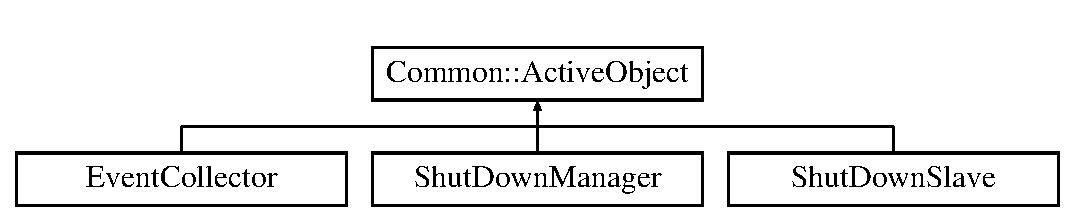
\includegraphics[height=2.000000cm]{class_common_1_1_active_object}
\end{center}
\end{figure}
\subsection*{Public Member Functions}
\begin{DoxyCompactItemize}
\item 
\hypertarget{class_common_1_1_active_object_ab695c61e3f83e29eede97c8c09308fb4}{\hyperlink{class_common_1_1_active_object_ab695c61e3f83e29eede97c8c09308fb4}{Active\-Object} ()}\label{class_common_1_1_active_object_ab695c61e3f83e29eede97c8c09308fb4}

\begin{DoxyCompactList}\small\item\em Constructor. \end{DoxyCompactList}\item 
\hypertarget{class_common_1_1_active_object_a69493bb331c7557aca8d3bd08203b086}{virtual \hyperlink{class_common_1_1_active_object_a69493bb331c7557aca8d3bd08203b086}{$\sim$\-Active\-Object} ()}\label{class_common_1_1_active_object_a69493bb331c7557aca8d3bd08203b086}

\begin{DoxyCompactList}\small\item\em Destructor. \end{DoxyCompactList}\item 
\hypertarget{class_common_1_1_active_object_ad39e4bb7a48b39470cbab48ab8ed11ff}{void \hyperlink{class_common_1_1_active_object_ad39e4bb7a48b39470cbab48ab8ed11ff}{Kill} ()}\label{class_common_1_1_active_object_ad39e4bb7a48b39470cbab48ab8ed11ff}

\begin{DoxyCompactList}\small\item\em Stops the thread execution. \end{DoxyCompactList}\end{DoxyCompactItemize}
\subsection*{Protected Member Functions}
\begin{DoxyCompactItemize}
\item 
\hypertarget{class_common_1_1_active_object_a9bc8d910184b23b25df7ac6dffa7e6e3}{virtual void {\bfseries Init\-Thread} ()=0}\label{class_common_1_1_active_object_a9bc8d910184b23b25df7ac6dffa7e6e3}

\item 
\hypertarget{class_common_1_1_active_object_aaaf7d59f7ca8efa8af210db47e3b56af}{virtual void {\bfseries Run} ()=0}\label{class_common_1_1_active_object_aaaf7d59f7ca8efa8af210db47e3b56af}

\item 
\hypertarget{class_common_1_1_active_object_af46d88184863861cdb921b2bac1ab458}{virtual void {\bfseries Flush\-Thread} ()=0}\label{class_common_1_1_active_object_af46d88184863861cdb921b2bac1ab458}

\item 
\hypertarget{class_common_1_1_active_object_a67a1764f49660a0d24c9b48671337f2d}{void \hyperlink{class_common_1_1_active_object_a67a1764f49660a0d24c9b48671337f2d}{Resume} ()}\label{class_common_1_1_active_object_a67a1764f49660a0d24c9b48671337f2d}

\begin{DoxyCompactList}\small\item\em Continues with the execution of the thread. \end{DoxyCompactList}\end{DoxyCompactItemize}
\subsection*{Protected Attributes}
\begin{DoxyCompactItemize}
\item 
\hypertarget{class_common_1_1_active_object_a8a1af686cb9455bd5fae334ff7e3e3cc}{int {\bfseries \-\_\-is\-Dying}}\label{class_common_1_1_active_object_a8a1af686cb9455bd5fae334ff7e3e3cc}

\end{DoxyCompactItemize}


\subsection{Detailed Description}
Abstract class, encapsulates O\-S thread (pthreads) P\-O\-S\-I\-X compatible. 

Last thing in the constructor of a class derived from \hyperlink{class_common_1_1_active_object}{Active\-Object} must be a call to {\itshape \-\_\-thread.\-Resume();}\par
 Inside the loop the Run method must keep checking {\itshape \-\_\-is\-Dying}\-: 
\begin{DoxyCode}
\textcolor{keywordflow}{if} (\_isDying)
    \textcolor{keywordflow}{return};
\end{DoxyCode}


\begin{DoxyVersion}{Version}
1.\-0b 
\end{DoxyVersion}
\begin{DoxySince}{Since}
1.\-0b 
\end{DoxySince}
\begin{DoxyAuthor}{Author}
Ania Sikora, 2002 
\end{DoxyAuthor}


The documentation for this class was generated from the following files\-:\begin{DoxyCompactItemize}
\item 
Common/Active\-Object.\-h\item 
Common/Active\-Object.\-cpp\end{DoxyCompactItemize}

\hypertarget{class_common_1_1_add_instr_request}{\section{Common\-:\-:Add\-Instr\-Request Class Reference}
\label{class_common_1_1_add_instr_request}\index{Common\-::\-Add\-Instr\-Request@{Common\-::\-Add\-Instr\-Request}}
}


Represents message sent when analyzer requests to add instrumentation.  




{\ttfamily \#include $<$P\-T\-P\-Msg.\-h$>$}

Inheritance diagram for Common\-:\-:Add\-Instr\-Request\-:\begin{figure}[H]
\begin{center}
\leavevmode
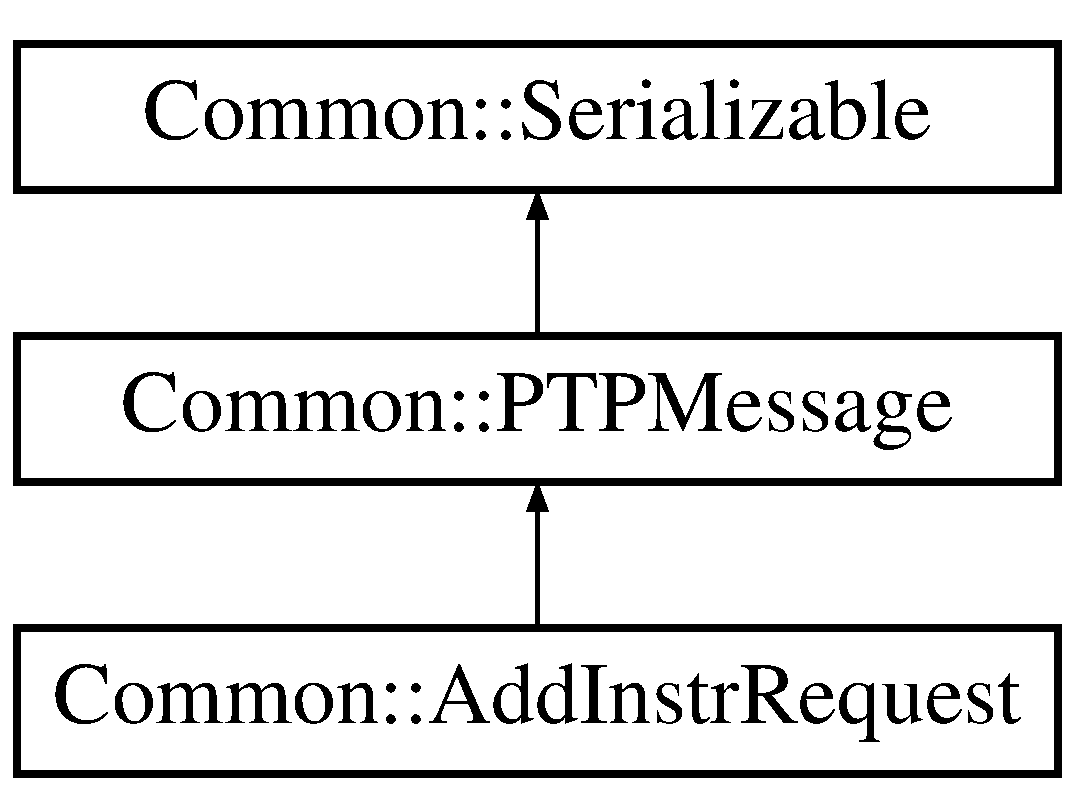
\includegraphics[height=3.000000cm]{class_common_1_1_add_instr_request}
\end{center}
\end{figure}
\subsection*{Public Member Functions}
\begin{DoxyCompactItemize}
\item 
\hyperlink{class_common_1_1_add_instr_request_a68a7aaf187b3d45a125f7de8ca76b780}{Add\-Instr\-Request} (int pid=0, int event\-Id=0, std\-::string const \&func\-Name=std\-::string(), Instr\-Place place=ip\-Func\-Entry, int n\-Attrs=0, \hyperlink{class_common_1_1_attribute}{Attribute} $\ast$attrs=0, int n\-Papi=0, std\-::string $\ast$Papi\-Metrics=0)
\begin{DoxyCompactList}\small\item\em Constructor. \end{DoxyCompactList}\item 
\hypertarget{class_common_1_1_add_instr_request_a9c4bdab0d2f8cb229a6057a25674672d}{\hyperlink{class_common_1_1_add_instr_request_a9c4bdab0d2f8cb229a6057a25674672d}{$\sim$\-Add\-Instr\-Request} ()}\label{class_common_1_1_add_instr_request_a9c4bdab0d2f8cb229a6057a25674672d}

\begin{DoxyCompactList}\small\item\em Destructor. \end{DoxyCompactList}\item 
\hypertarget{class_common_1_1_add_instr_request_a9c1b7191b6289cc9b724d06428601b4b}{P\-T\-P\-Msg\-Type \hyperlink{class_common_1_1_add_instr_request_a9c1b7191b6289cc9b724d06428601b4b}{Get\-Type} () const }\label{class_common_1_1_add_instr_request_a9c1b7191b6289cc9b724d06428601b4b}

\begin{DoxyCompactList}\small\item\em Returns type of message (P\-T\-P\-Add\-Instr). \end{DoxyCompactList}\item 
\hypertarget{class_common_1_1_add_instr_request_aeff18bc4bbbdd7e5df05d6ed697446e0}{int \hyperlink{class_common_1_1_add_instr_request_aeff18bc4bbbdd7e5df05d6ed697446e0}{Get\-Pid} () const }\label{class_common_1_1_add_instr_request_aeff18bc4bbbdd7e5df05d6ed697446e0}

\begin{DoxyCompactList}\small\item\em Returns the process id. \end{DoxyCompactList}\item 
\hypertarget{class_common_1_1_add_instr_request_ac4799ac58ff77a45b4980478a04dd0b4}{Instr\-Place \hyperlink{class_common_1_1_add_instr_request_ac4799ac58ff77a45b4980478a04dd0b4}{Get\-Instr\-Place} () const }\label{class_common_1_1_add_instr_request_ac4799ac58ff77a45b4980478a04dd0b4}

\begin{DoxyCompactList}\small\item\em Returns the place where the instruction should be added. \end{DoxyCompactList}\item 
\hypertarget{class_common_1_1_add_instr_request_af7a0c2f2796725b544d32c1fdb3983af}{std\-::string const \& \hyperlink{class_common_1_1_add_instr_request_af7a0c2f2796725b544d32c1fdb3983af}{Get\-Function\-Name} () const }\label{class_common_1_1_add_instr_request_af7a0c2f2796725b544d32c1fdb3983af}

\begin{DoxyCompactList}\small\item\em Returns function name. \end{DoxyCompactList}\item 
\hypertarget{class_common_1_1_add_instr_request_a2b426cdee36bb34befd7c352e311b091}{int \hyperlink{class_common_1_1_add_instr_request_a2b426cdee36bb34befd7c352e311b091}{Get\-Event\-Id} () const }\label{class_common_1_1_add_instr_request_a2b426cdee36bb34befd7c352e311b091}

\begin{DoxyCompactList}\small\item\em Returns the event id. \end{DoxyCompactList}\item 
\hypertarget{class_common_1_1_add_instr_request_a8641c2ae4a2a32535fb73be25ef39eb9}{\hyperlink{class_common_1_1_attribute}{Attribute} $\ast$ \hyperlink{class_common_1_1_add_instr_request_a8641c2ae4a2a32535fb73be25ef39eb9}{Get\-Attributes} () const }\label{class_common_1_1_add_instr_request_a8641c2ae4a2a32535fb73be25ef39eb9}

\begin{DoxyCompactList}\small\item\em Returns array of attributes. \end{DoxyCompactList}\item 
\hypertarget{class_common_1_1_add_instr_request_a969ac38ec14c83e16cbc9c74527f4121}{int \hyperlink{class_common_1_1_add_instr_request_a969ac38ec14c83e16cbc9c74527f4121}{Get\-Attrs\-Count} () const }\label{class_common_1_1_add_instr_request_a969ac38ec14c83e16cbc9c74527f4121}

\begin{DoxyCompactList}\small\item\em Returns number of attributes the function has. \end{DoxyCompactList}\item 
\hypertarget{class_common_1_1_add_instr_request_a5a19a930c393f48dce79c123ca1258ab}{std\-::string $\ast$ \hyperlink{class_common_1_1_add_instr_request_a5a19a930c393f48dce79c123ca1258ab}{Get\-Metrics} () const }\label{class_common_1_1_add_instr_request_a5a19a930c393f48dce79c123ca1258ab}

\begin{DoxyCompactList}\small\item\em Returns array of Metrics. \end{DoxyCompactList}\item 
\hypertarget{class_common_1_1_add_instr_request_a2754506cc3c0fe7d7e850199f9857f41}{int \hyperlink{class_common_1_1_add_instr_request_a2754506cc3c0fe7d7e850199f9857f41}{Get\-Metrics\-Count} () const }\label{class_common_1_1_add_instr_request_a2754506cc3c0fe7d7e850199f9857f41}

\begin{DoxyCompactList}\small\item\em Returns number of metrics the function has. \end{DoxyCompactList}\item 
\hypertarget{class_common_1_1_add_instr_request_a8405b78cf676da3be84514b7838665ee}{void \hyperlink{class_common_1_1_add_instr_request_a8405b78cf676da3be84514b7838665ee}{Serialize} (\hyperlink{class_common_1_1_serializer}{Serializer} \&out) const }\label{class_common_1_1_add_instr_request_a8405b78cf676da3be84514b7838665ee}

\begin{DoxyCompactList}\small\item\em Sends the message. \end{DoxyCompactList}\item 
\hypertarget{class_common_1_1_add_instr_request_a09b4fde5119b8f7ba662cfe38b195e4a}{void \hyperlink{class_common_1_1_add_instr_request_a09b4fde5119b8f7ba662cfe38b195e4a}{De\-Serialize} (\hyperlink{class_common_1_1_de_serializer}{De\-Serializer} \&in)}\label{class_common_1_1_add_instr_request_a09b4fde5119b8f7ba662cfe38b195e4a}

\begin{DoxyCompactList}\small\item\em Receives the message. \end{DoxyCompactList}\end{DoxyCompactItemize}


\subsection{Detailed Description}
Represents message sent when analyzer requests to add instrumentation. 

\begin{DoxyVersion}{Version}
1.\-0b 
\end{DoxyVersion}
\begin{DoxySince}{Since}
1.\-0b 
\end{DoxySince}
\begin{DoxyAuthor}{Author}
Ania Sikora, 2003 
\end{DoxyAuthor}


\subsection{Constructor \& Destructor Documentation}
\hypertarget{class_common_1_1_add_instr_request_a68a7aaf187b3d45a125f7de8ca76b780}{\index{Common\-::\-Add\-Instr\-Request@{Common\-::\-Add\-Instr\-Request}!Add\-Instr\-Request@{Add\-Instr\-Request}}
\index{Add\-Instr\-Request@{Add\-Instr\-Request}!Common::AddInstrRequest@{Common\-::\-Add\-Instr\-Request}}
\subsubsection[{Add\-Instr\-Request}]{\setlength{\rightskip}{0pt plus 5cm}Common\-::\-Add\-Instr\-Request\-::\-Add\-Instr\-Request (
\begin{DoxyParamCaption}
\item[{int}]{pid = {\ttfamily 0}, }
\item[{int}]{event\-Id = {\ttfamily 0}, }
\item[{std\-::string const \&}]{func\-Name = {\ttfamily std\-:\-:string()}, }
\item[{Instr\-Place}]{place = {\ttfamily ipFuncEntry}, }
\item[{int}]{n\-Attrs = {\ttfamily 0}, }
\item[{{\bf Attribute} $\ast$}]{attrs = {\ttfamily 0}, }
\item[{int}]{n\-Papi = {\ttfamily 0}, }
\item[{std\-::string $\ast$}]{Papi\-Metrics = {\ttfamily 0}}
\end{DoxyParamCaption}
)\hspace{0.3cm}{\ttfamily [inline]}}}\label{class_common_1_1_add_instr_request_a68a7aaf187b3d45a125f7de8ca76b780}


Constructor. 


\begin{DoxyParams}{Parameters}
{\em pid} & Id of the process where the instrumentation will be added, default 0. \\
\hline
{\em event\-Id} & \hyperlink{class_common_1_1_event}{Event} id, default 0. \\
\hline
{\em func\-Name} & Name of the function to modify, default \char`\"{}\char`\"{}. \\
\hline
{\em place} & Place where the instrumentation will be added, default ip\-Func\-Entry. \\
\hline
{\em n\-Attrs} & Number of attributes the function has, default 0. \\
\hline
{\em attrs} & \hyperlink{class_common_1_1_attribute}{Attribute} array, default 0. \\
\hline
\end{DoxyParams}


The documentation for this class was generated from the following files\-:\begin{DoxyCompactItemize}
\item 
Common/P\-T\-P\-Msg.\-h\item 
Common/P\-T\-P\-Msg.\-cpp\end{DoxyCompactItemize}

\hypertarget{class_common_1_1_address}{\section{Common\-:\-:Address Class Reference}
\label{class_common_1_1_address}\index{Common\-::\-Address@{Common\-::\-Address}}
}


Encapsulates a socket address of the A\-F\-\_\-\-I\-N\-E\-T family.  




{\ttfamily \#include $<$Address.\-h$>$}

\subsection*{Public Member Functions}
\begin{DoxyCompactItemize}
\item 
\hyperlink{class_common_1_1_address_a94cc0e4607b6124a926cb1f27792cf62}{Address} (std\-::string const \&host, int port)
\begin{DoxyCompactList}\small\item\em Constructor. \end{DoxyCompactList}\item 
\hyperlink{class_common_1_1_address_a4dc926540c01072ed3a064623a135341}{Address} (int port)
\begin{DoxyCompactList}\small\item\em Constructor. \end{DoxyCompactList}\item 
\hyperlink{class_common_1_1_address_a63f910c09d93bdd16d3744e47d13dc0e}{Address} ()
\begin{DoxyCompactList}\small\item\em Constructor. \end{DoxyCompactList}\item 
\hypertarget{class_common_1_1_address_ac763a8750a054f589297f6a2994fdd16}{\hyperlink{class_common_1_1_address_ac763a8750a054f589297f6a2994fdd16}{operator struct sockaddr $\ast$} ()}\label{class_common_1_1_address_ac763a8750a054f589297f6a2994fdd16}

\begin{DoxyCompactList}\small\item\em Returns a pointer to the sockaddr intern structure. \end{DoxyCompactList}\item 
\hypertarget{class_common_1_1_address_a16f9cd6303d3c150c1a040b043f4897f}{\hyperlink{class_common_1_1_address_a16f9cd6303d3c150c1a040b043f4897f}{operator struct sockaddr\-\_\-in $\ast$} ()}\label{class_common_1_1_address_a16f9cd6303d3c150c1a040b043f4897f}

\begin{DoxyCompactList}\small\item\em Returns a pointer to the sockaddr\-\_\-in intern structure. \end{DoxyCompactList}\item 
\hypertarget{class_common_1_1_address_abc84f0684263e6d58482b972916e6747}{socklen\-\_\-t \hyperlink{class_common_1_1_address_abc84f0684263e6d58482b972916e6747}{Get\-Size} () const }\label{class_common_1_1_address_abc84f0684263e6d58482b972916e6747}

\begin{DoxyCompactList}\small\item\em Returns size of current address. Number of bytes the address uses in memory. \end{DoxyCompactList}\item 
std\-::string \hyperlink{class_common_1_1_address_a4e368d46d4e8fbb9032cdff4e921db94}{Get\-Host\-Name} () const 
\begin{DoxyCompactList}\small\item\em Returns name of host. \end{DoxyCompactList}\end{DoxyCompactItemize}


\subsection{Detailed Description}
Encapsulates a socket address of the A\-F\-\_\-\-I\-N\-E\-T family. 

This class contains methods to initialize the address of a socket.

\begin{DoxyVersion}{Version}
1.\-0b 
\end{DoxyVersion}
\begin{DoxySince}{Since}
1.\-0b 
\end{DoxySince}
\begin{DoxyAuthor}{Author}
Ania Sikora, 2002 
\end{DoxyAuthor}


\subsection{Constructor \& Destructor Documentation}
\hypertarget{class_common_1_1_address_a94cc0e4607b6124a926cb1f27792cf62}{\index{Common\-::\-Address@{Common\-::\-Address}!Address@{Address}}
\index{Address@{Address}!Common::Address@{Common\-::\-Address}}
\subsubsection[{Address}]{\setlength{\rightskip}{0pt plus 5cm}Common\-::\-Address\-::\-Address (
\begin{DoxyParamCaption}
\item[{std\-::string const \&}]{host, }
\item[{int}]{port}
\end{DoxyParamCaption}
)}}\label{class_common_1_1_address_a94cc0e4607b6124a926cb1f27792cf62}


Constructor. 


\begin{DoxyParams}{Parameters}
{\em host} & Host where the socket will be located. \\
\hline
{\em port} & Port used.\\
\hline
\end{DoxyParams}

\begin{DoxyExceptions}{Exceptions}
{\em \hyperlink{class_common_1_1_sys_exception}{Sys\-Exception}} & \\
\hline
\end{DoxyExceptions}
\hypertarget{class_common_1_1_address_a4dc926540c01072ed3a064623a135341}{\index{Common\-::\-Address@{Common\-::\-Address}!Address@{Address}}
\index{Address@{Address}!Common::Address@{Common\-::\-Address}}
\subsubsection[{Address}]{\setlength{\rightskip}{0pt plus 5cm}Address\-::\-Address (
\begin{DoxyParamCaption}
\item[{int}]{port}
\end{DoxyParamCaption}
)}}\label{class_common_1_1_address_a4dc926540c01072ed3a064623a135341}


Constructor. 

Uses the I\-N\-A\-D\-D\-R\-\_\-\-A\-N\-Y address.


\begin{DoxyParams}{Parameters}
{\em port} & Port used. \\
\hline
\end{DoxyParams}
\hypertarget{class_common_1_1_address_a63f910c09d93bdd16d3744e47d13dc0e}{\index{Common\-::\-Address@{Common\-::\-Address}!Address@{Address}}
\index{Address@{Address}!Common::Address@{Common\-::\-Address}}
\subsubsection[{Address}]{\setlength{\rightskip}{0pt plus 5cm}Address\-::\-Address (
\begin{DoxyParamCaption}
{}
\end{DoxyParamCaption}
)}}\label{class_common_1_1_address_a63f910c09d93bdd16d3744e47d13dc0e}


Constructor. 

Initializes an empty address, setting the memory of the object to 0. 

\subsection{Member Function Documentation}
\hypertarget{class_common_1_1_address_a4e368d46d4e8fbb9032cdff4e921db94}{\index{Common\-::\-Address@{Common\-::\-Address}!Get\-Host\-Name@{Get\-Host\-Name}}
\index{Get\-Host\-Name@{Get\-Host\-Name}!Common::Address@{Common\-::\-Address}}
\subsubsection[{Get\-Host\-Name}]{\setlength{\rightskip}{0pt plus 5cm}string Address\-::\-Get\-Host\-Name (
\begin{DoxyParamCaption}
{}
\end{DoxyParamCaption}
) const}}\label{class_common_1_1_address_a4e368d46d4e8fbb9032cdff4e921db94}


Returns name of host. 


\begin{DoxyExceptions}{Exceptions}
{\em \hyperlink{class_common_1_1_sys_exception}{Sys\-Exception}} & \\
\hline
\end{DoxyExceptions}


The documentation for this class was generated from the following files\-:\begin{DoxyCompactItemize}
\item 
Common/Address.\-h\item 
Common/Address.\-cpp\end{DoxyCompactItemize}

\hypertarget{class_analyzer}{\section{Analyzer Class Reference}
\label{class_analyzer}\index{Analyzer@{Analyzer}}
}


Analyzes events from a given set and determines if there are problems within them. The class also has the capabilities to add or remove instrumentation from the code.  




{\ttfamily \#include $<$Analyzer.\-h$>$}

\subsection*{Public Member Functions}
\begin{DoxyCompactItemize}
\item 
\hyperlink{class_analyzer_a297d271be87a5119ccc5963da55d3e69}{Analyzer} (Event\-List \&list)
\begin{DoxyCompactList}\small\item\em Constructor. \end{DoxyCompactList}\item 
\hypertarget{class_analyzer_a7186b1dd005cea7f0c3de1d74da00184}{void \hyperlink{class_analyzer_a7186b1dd005cea7f0c3de1d74da00184}{Analyze\-Event} ()}\label{class_analyzer_a7186b1dd005cea7f0c3de1d74da00184}

\begin{DoxyCompactList}\small\item\em Analyzes an event and, if it finds a problem, makes tuning actions. \end{DoxyCompactList}\item 
\hypertarget{class_analyzer_a74273bc7c5f368bbf1fcf748d68b0462}{void \hyperlink{class_analyzer_a74273bc7c5f368bbf1fcf748d68b0462}{Instrument} ()}\label{class_analyzer_a74273bc7c5f368bbf1fcf748d68b0462}

\begin{DoxyCompactList}\small\item\em Requests to add instrumentation in the application so as to get information from it. \end{DoxyCompactList}\item 
\hypertarget{class_analyzer_a6c8d3c336db431f01ce2cfd0d4546af8}{void \hyperlink{class_analyzer_a6c8d3c336db431f01ce2cfd0d4546af8}{Remove\-Instr} ()}\label{class_analyzer_a6c8d3c336db431f01ce2cfd0d4546af8}

\begin{DoxyCompactList}\small\item\em Requests to remove instrumentation. \end{DoxyCompactList}\item 
\hypertarget{class_analyzer_a8a4df19454f1a93f020c8062cdd93423}{void \hyperlink{class_analyzer_a8a4df19454f1a93f020c8062cdd93423}{Tune} ()}\label{class_analyzer_a8a4df19454f1a93f020c8062cdd93423}

\begin{DoxyCompactList}\small\item\em Requests to modify the application in order to improve its behavior. \end{DoxyCompactList}\end{DoxyCompactItemize}


\subsection{Detailed Description}
Analyzes events from a given set and determines if there are problems within them. The class also has the capabilities to add or remove instrumentation from the code. 

\begin{DoxyVersion}{Version}
1.\-0b 
\end{DoxyVersion}
\begin{DoxyAuthor}{Author}
Ania Sikora, 2002 
\end{DoxyAuthor}
\begin{DoxySince}{Since}
1.\-0b 
\end{DoxySince}


\subsection{Constructor \& Destructor Documentation}
\hypertarget{class_analyzer_a297d271be87a5119ccc5963da55d3e69}{\index{Analyzer@{Analyzer}!Analyzer@{Analyzer}}
\index{Analyzer@{Analyzer}!Analyzer@{Analyzer}}
\subsubsection[{Analyzer}]{\setlength{\rightskip}{0pt plus 5cm}Analyzer\-::\-Analyzer (
\begin{DoxyParamCaption}
\item[{Event\-List \&}]{list}
\end{DoxyParamCaption}
)\hspace{0.3cm}{\ttfamily [inline]}}}\label{class_analyzer_a297d271be87a5119ccc5963da55d3e69}


Constructor. 


\begin{DoxyParams}{Parameters}
{\em list} & of events to be analyzed \\
\hline
\end{DoxyParams}


The documentation for this class was generated from the following files\-:\begin{DoxyCompactItemize}
\item 
Analyzer/Analyzer.\-h\item 
Analyzer/Analyzer.\-cpp\end{DoxyCompactItemize}

\hypertarget{class_model_1_1_application}{\section{Model\-:\-:Application Class Reference}
\label{class_model_1_1_application}\index{Model\-::\-Application@{Model\-::\-Application}}
}


Represents tuned application in the analyzer. Holds identificative information of the application, the tasks that form it (and which one is the master), the host where they are running, the places from where we are getting events and handlers to both\-: tasks and hosts. Provides methods to\-:  




{\ttfamily \#include $<$App\-Model.\-h$>$}

Inheritance diagram for Model\-:\-:Application\-:\begin{figure}[H]
\begin{center}
\leavevmode
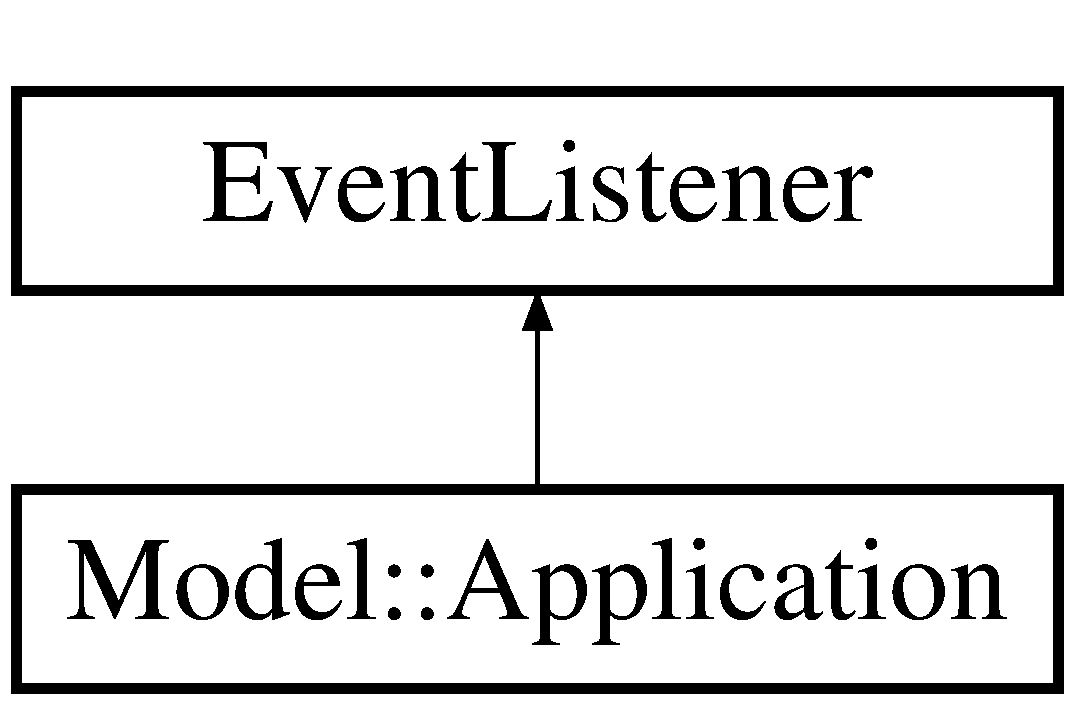
\includegraphics[height=2.000000cm]{class_model_1_1_application}
\end{center}
\end{figure}
\subsection*{Public Member Functions}
\begin{DoxyCompactItemize}
\item 
\hyperlink{class_model_1_1_application_a817618af167f7af002f1cbdf4d4c38b2}{Application} (char const $\ast$app\-Path, int argc, char const $\ast$$\ast$argv)
\begin{DoxyCompactList}\small\item\em Constructor. \end{DoxyCompactList}\item 
string \hyperlink{class_model_1_1_application_a9711ebdc4fb083bcd94f553fdda76fc6}{Get\-Name} () const 
\begin{DoxyCompactList}\small\item\em Name getter. \end{DoxyCompactList}\item 
int \hyperlink{class_model_1_1_application_a854cc5e17c6b50afe94ef9874390c43e}{Num\-Active\-Tasks} () const 
\begin{DoxyCompactList}\small\item\em Number of tasks getter. \end{DoxyCompactList}\item 
\hyperlink{class_model_1_1_tasks}{Tasks} \& \hyperlink{class_model_1_1_application_a1266983b65e6fde4203e8b224f1ed9ba}{Get\-Tasks} ()
\begin{DoxyCompactList}\small\item\em \hyperlink{class_model_1_1_tasks}{Tasks} getter. \end{DoxyCompactList}\item 
\hyperlink{classauto__vector}{Hosts} \& \hyperlink{class_model_1_1_application_ae8c12c9613d83d32302bf19908cf812a}{Get\-Hosts} ()
\begin{DoxyCompactList}\small\item\em Hosts getter. \end{DoxyCompactList}\item 
\hyperlink{class_model_1_1_task}{Task} $\ast$ \hyperlink{class_model_1_1_application_aeb0ce50463e62a7009a5d316c3d2feed}{Get\-Master\-Task} ()
\begin{DoxyCompactList}\small\item\em Master task getter. \end{DoxyCompactList}\item 
Status \hyperlink{class_model_1_1_application_afdc09d44cad811cfaa90a53dd1039247}{Get\-Status} () const 
\item 
void \hyperlink{class_model_1_1_application_adedfa7e821be70b6c9f47086cdaade1d}{Start} ()
\begin{DoxyCompactList}\small\item\em Starts the application. \end{DoxyCompactList}\item 
int \hyperlink{class_model_1_1_application_ae18bdad6563f77fe5a2809c95b62b904}{Add\-Event} (\hyperlink{class_model_1_1_event}{Event} const \&e)
\begin{DoxyCompactList}\small\item\em Adds a definition of a new event to be traced in all running tasks of the application. \end{DoxyCompactList}\item 
int \hyperlink{class_model_1_1_application_a25e5cc464e72a9d89568a0887037cd86}{Remove\-Event} (int event\-Id, Instr\-Place place)
\begin{DoxyCompactList}\small\item\em Removes previously added event from all running tasks. \end{DoxyCompactList}\item 
int \hyperlink{class_model_1_1_application_a8f7a91af569e21f367ba5b01ad33cd17}{Load\-Library} (string const \&lib\-Path)
\begin{DoxyCompactList}\small\item\em Loads a shared library to all running tasks. This enables the \hyperlink{class_analyzer}{Analyzer} to load any additional code required for the tuning. \end{DoxyCompactList}\item 
int \hyperlink{class_model_1_1_application_ab7d662a340d96d28b1cced1cb7cbf528}{Set\-Variable\-Value} (string const \&var\-Name, \hyperlink{class_common_1_1_attribute_value}{Attribute\-Value} const \&var\-Value, \hyperlink{class_common_1_1_breakpoint}{Breakpoint} $\ast$brkpt)
\begin{DoxyCompactList}\small\item\em Modifies a value of a specified variable in a given set of tasks. \end{DoxyCompactList}\item 
int \hyperlink{class_model_1_1_application_ab18ecde3fa6610b6f5d50190a869dc66}{Replace\-Function} (string const \&old\-Func, string const \&new\-Func, \hyperlink{class_common_1_1_breakpoint}{Breakpoint} $\ast$brkpt)
\begin{DoxyCompactList}\small\item\em Replaces all calls to a function with calls to another one in a given set of tasks. \end{DoxyCompactList}\item 
int \hyperlink{class_model_1_1_application_aba1d7b1c80c8454a9fab16ef429a002c}{Insert\-Function\-Call} (string const \&func\-Name, int n\-Attrs, \hyperlink{class_common_1_1_attribute}{Attribute} $\ast$attrs, string const \&dest\-Func, Instr\-Place dest\-Place, \hyperlink{class_common_1_1_breakpoint}{Breakpoint} $\ast$brkpt)
\begin{DoxyCompactList}\small\item\em Inserts a new function invocation code at a given location in a given set of tasks. \end{DoxyCompactList}\item 
int \hyperlink{class_model_1_1_application_aeca69d9264c3e75f9339e7a58aa0ffd8}{One\-Time\-Func\-Call} (string const \&func\-Name, int n\-Attrs, \hyperlink{class_common_1_1_attribute}{Attribute} $\ast$attrs, \hyperlink{class_common_1_1_breakpoint}{Breakpoint} $\ast$brkpt)
\begin{DoxyCompactList}\small\item\em Inserts a new function invocation code in a given set of tasks and calls it once. \end{DoxyCompactList}\item 
int \hyperlink{class_model_1_1_application_a0e2c20e91428dd90c67928dfc3437576}{Remove\-Func\-Call} (string const \&func\-Name, string const \&caller\-Func, \hyperlink{class_common_1_1_breakpoint}{Breakpoint} $\ast$brkpt)
\begin{DoxyCompactList}\small\item\em Removes all calls to a given function from the given caller function in a given set of tasks. For example this method can be used to remove all flush() function calls from a debug() function. \end{DoxyCompactList}\item 
int \hyperlink{class_model_1_1_application_a1ce4864393ec35b5bd705b42890d4961}{Func\-Param\-Change} (string const \&func\-Name, int param\-Idx, int new\-Value, int $\ast$required\-Old\-Value, \hyperlink{class_common_1_1_breakpoint}{Breakpoint} $\ast$brkpt)
\begin{DoxyCompactList}\small\item\em Sets the value of an input parameter of a given function in a given set of tasks. This parameter value is modified before the function body is invoked. There exists the possibility to change the parameter value under condition, namely if the parameter has a value equal to required\-Old\-Value, only then its value is changed to new one. If the required\-Old\-Value is zero, then the value of the parameter is changed unconditionally. \end{DoxyCompactList}\item 
void \hyperlink{class_model_1_1_application_a05110a6e0973b2b9a55b575c84f49357}{Set\-Task\-Handler} (\hyperlink{class_model_1_1_task_handler}{Task\-Handler} \&h)
\begin{DoxyCompactList}\small\item\em Installs a callback function that is called when a new task is started or an existing one is terminated. \end{DoxyCompactList}\item 
void \hyperlink{class_model_1_1_application_a9470d1cac97d3e0a11bddc730889a04c}{Set\-Host\-Handler} (\hyperlink{class_model_1_1_host_handler}{Host\-Handler} \&h)
\begin{DoxyCompactList}\small\item\em Installs a callback function that is called when a new host is added to the virtual machine or an existing one is removed. \end{DoxyCompactList}\item 
int \hyperlink{class_model_1_1_application_a7a7aa1fa007d9bd77fd9d903883bf836}{Process\-Events} (bool block=true)
\begin{DoxyCompactList}\small\item\em Processes application events (E\-C\-P). \end{DoxyCompactList}\item 
void \hyperlink{class_model_1_1_application_aeb4e28cb6431a3b073dcf379731ec614}{On\-Event} (\hyperlink{class_common_1_1_e_c_p_message}{E\-C\-P\-Message} $\ast$msg)
\begin{DoxyCompactList}\small\item\em This method is called in the context of \hyperlink{class_model_1_1_event}{Event} Collector thread. \end{DoxyCompactList}\item 
\hypertarget{class_model_1_1_application_a9c94ac7dbdaebe7719995be26826310b}{void \hyperlink{class_model_1_1_application_a9c94ac7dbdaebe7719995be26826310b}{On\-Fatal\-Error} ()}\label{class_model_1_1_application_a9c94ac7dbdaebe7719995be26826310b}

\begin{DoxyCompactList}\small\item\em This method is called when fatal \hyperlink{class_event_collector}{Event\-Collector} error occurs. \hyperlink{class_model_1_1_application}{Application} changes its status to st\-Aborted. \end{DoxyCompactList}\end{DoxyCompactItemize}
\subsection*{Protected Member Functions}
\begin{DoxyCompactItemize}
\item 
void \hyperlink{class_model_1_1_application_a5d3109b0e0220d8ccdf68ca3a6a9dbd1}{Process\-Event} (\hyperlink{class_common_1_1_e_c_p_message}{E\-C\-P\-Message} $\ast$msg)
\begin{DoxyCompactList}\small\item\em Takes the proper actions depending on the kind of message received. \end{DoxyCompactList}\item 
void \hyperlink{class_model_1_1_application_a07458796fbf3b7ec4880cdecd74955a7}{Dispatch\-Event} (\hyperlink{class_common_1_1_event_msg}{Event\-Msg} const \&msg)
\begin{DoxyCompactList}\small\item\em Finds the sender-\/task corresponding object and dispatches its event (see task). \end{DoxyCompactList}\item 
\hyperlink{class_model_1_1_host}{Host} \& \hyperlink{class_model_1_1_application_ac1a97bc607a531c995781b227a974964}{Add\-Host} (string const \&name)
\begin{DoxyCompactList}\small\item\em Creates \& adds a new host to the host list of the application. \end{DoxyCompactList}\item 
void \hyperlink{class_model_1_1_application_a2984c77612af632e4908876f240b3a5b}{Add\-Task} (int pid, int mpi\-Rank, string const \&name, \hyperlink{class_model_1_1_host}{Host} \&h)
\begin{DoxyCompactList}\small\item\em Adds a task to the application list. \end{DoxyCompactList}\item 
void \hyperlink{class_model_1_1_application_a4fad9da559357f9187c23a3bf76a69bf}{Remove\-Task} (int tid)
\begin{DoxyCompactList}\small\item\em Removes a task when an unregistered message is received (see process\-Event). \end{DoxyCompactList}\end{DoxyCompactItemize}


\subsection{Detailed Description}
Represents tuned application in the analyzer. Holds identificative information of the application, the tasks that form it (and which one is the master), the host where they are running, the places from where we are getting events and handlers to both\-: tasks and hosts. Provides methods to\-: 


\begin{DoxyItemize}
\item Retrieve application information 
\item Monitoring\-: add/remove events to trace. 
\item Tuning\-: loading libraries, changing variables \& parameter values, adding/removing function calls and calling them explicitly.  
\end{DoxyItemize}Basically the monitoring a tuning methods call to the corresponding methods in App\-Task for all the tasks that conform the application. 

\subsection{Constructor \& Destructor Documentation}
\hypertarget{class_model_1_1_application_a817618af167f7af002f1cbdf4d4c38b2}{\index{Model\-::\-Application@{Model\-::\-Application}!Application@{Application}}
\index{Application@{Application}!Model::Application@{Model\-::\-Application}}
\subsubsection[{Application}]{\setlength{\rightskip}{0pt plus 5cm}Application\-::\-Application (
\begin{DoxyParamCaption}
\item[{char const $\ast$}]{app\-Path, }
\item[{int}]{argc, }
\item[{char const $\ast$$\ast$}]{argv}
\end{DoxyParamCaption}
)}}\label{class_model_1_1_application_a817618af167f7af002f1cbdf4d4c38b2}


Constructor. 


\begin{DoxyParams}{Parameters}
{\em app\-Path} & Path to the executable of the application. \\
\hline
{\em argc} & Number of arguments of the application. \\
\hline
{\em argv} & Arguments of the application. \\
\hline
\end{DoxyParams}


\subsection{Member Function Documentation}
\hypertarget{class_model_1_1_application_ae18bdad6563f77fe5a2809c95b62b904}{\index{Model\-::\-Application@{Model\-::\-Application}!Add\-Event@{Add\-Event}}
\index{Add\-Event@{Add\-Event}!Model::Application@{Model\-::\-Application}}
\subsubsection[{Add\-Event}]{\setlength{\rightskip}{0pt plus 5cm}int Application\-::\-Add\-Event (
\begin{DoxyParamCaption}
\item[{{\bf Event} const \&}]{e}
\end{DoxyParamCaption}
)}}\label{class_model_1_1_application_ae18bdad6563f77fe5a2809c95b62b904}


Adds a definition of a new event to be traced in all running tasks of the application. 


\begin{DoxyParams}{Parameters}
{\em e} & \hyperlink{class_model_1_1_event}{Event} to be traced. \\
\hline
\end{DoxyParams}
\begin{DoxyReturn}{Returns}
Number of tasks where the event tracing was added. 
\end{DoxyReturn}
\hypertarget{class_model_1_1_application_ac1a97bc607a531c995781b227a974964}{\index{Model\-::\-Application@{Model\-::\-Application}!Add\-Host@{Add\-Host}}
\index{Add\-Host@{Add\-Host}!Model::Application@{Model\-::\-Application}}
\subsubsection[{Add\-Host}]{\setlength{\rightskip}{0pt plus 5cm}{\bf Host} \& Application\-::\-Add\-Host (
\begin{DoxyParamCaption}
\item[{string const \&}]{name}
\end{DoxyParamCaption}
)\hspace{0.3cm}{\ttfamily [protected]}}}\label{class_model_1_1_application_ac1a97bc607a531c995781b227a974964}


Creates \& adds a new host to the host list of the application. 


\begin{DoxyParams}{Parameters}
{\em name} & Name of the host \\
\hline
\end{DoxyParams}
\begin{DoxyReturn}{Returns}
Reference to the created host 
\end{DoxyReturn}
\hypertarget{class_model_1_1_application_a2984c77612af632e4908876f240b3a5b}{\index{Model\-::\-Application@{Model\-::\-Application}!Add\-Task@{Add\-Task}}
\index{Add\-Task@{Add\-Task}!Model::Application@{Model\-::\-Application}}
\subsubsection[{Add\-Task}]{\setlength{\rightskip}{0pt plus 5cm}void Application\-::\-Add\-Task (
\begin{DoxyParamCaption}
\item[{int}]{pid, }
\item[{int}]{mpi\-Rank, }
\item[{string const \&}]{name, }
\item[{{\bf Host} \&}]{h}
\end{DoxyParamCaption}
)\hspace{0.3cm}{\ttfamily [protected]}}}\label{class_model_1_1_application_a2984c77612af632e4908876f240b3a5b}


Adds a task to the application list. 


\begin{DoxyParams}{Parameters}
{\em pid} & Process identifier of the task. \\
\hline
{\em mpi\-Rank} & M\-P\-I identifier of the task \\
\hline
{\em name} & Process name \\
\hline
{\em host} & \hyperlink{class_model_1_1_host}{Host} where the task is running \\
\hline
\end{DoxyParams}
\hypertarget{class_model_1_1_application_a07458796fbf3b7ec4880cdecd74955a7}{\index{Model\-::\-Application@{Model\-::\-Application}!Dispatch\-Event@{Dispatch\-Event}}
\index{Dispatch\-Event@{Dispatch\-Event}!Model::Application@{Model\-::\-Application}}
\subsubsection[{Dispatch\-Event}]{\setlength{\rightskip}{0pt plus 5cm}void Application\-::\-Dispatch\-Event (
\begin{DoxyParamCaption}
\item[{{\bf Event\-Msg} const \&}]{msg}
\end{DoxyParamCaption}
)\hspace{0.3cm}{\ttfamily [protected]}}}\label{class_model_1_1_application_a07458796fbf3b7ec4880cdecd74955a7}


Finds the sender-\/task corresponding object and dispatches its event (see task). 


\begin{DoxyParams}{Parameters}
{\em msg} & Message that contains an event request from an A\-C. \\
\hline
\end{DoxyParams}
\hypertarget{class_model_1_1_application_a1ce4864393ec35b5bd705b42890d4961}{\index{Model\-::\-Application@{Model\-::\-Application}!Func\-Param\-Change@{Func\-Param\-Change}}
\index{Func\-Param\-Change@{Func\-Param\-Change}!Model::Application@{Model\-::\-Application}}
\subsubsection[{Func\-Param\-Change}]{\setlength{\rightskip}{0pt plus 5cm}int Application\-::\-Func\-Param\-Change (
\begin{DoxyParamCaption}
\item[{string const \&}]{func\-Name, }
\item[{int}]{param\-Idx, }
\item[{int}]{new\-Value, }
\item[{int $\ast$}]{required\-Old\-Value, }
\item[{{\bf Breakpoint} $\ast$}]{brkpt}
\end{DoxyParamCaption}
)}}\label{class_model_1_1_application_a1ce4864393ec35b5bd705b42890d4961}


Sets the value of an input parameter of a given function in a given set of tasks. This parameter value is modified before the function body is invoked. There exists the possibility to change the parameter value under condition, namely if the parameter has a value equal to required\-Old\-Value, only then its value is changed to new one. If the required\-Old\-Value is zero, then the value of the parameter is changed unconditionally. 


\begin{DoxyParams}{Parameters}
{\em func\-Name} & Name of the function \\
\hline
{\em param\-Idx} & Id of the parameter to change \\
\hline
{\em new\-Value} & New value for the parameter \\
\hline
{\em required\-Old\-Value} & Required old value of the parameter to change it \\
\hline
{\em brkpt} & --- \\
\hline
\end{DoxyParams}
\begin{DoxyReturn}{Returns}
Number of tasks where the parameter was changed. 
\end{DoxyReturn}
\hypertarget{class_model_1_1_application_ae8c12c9613d83d32302bf19908cf812a}{\index{Model\-::\-Application@{Model\-::\-Application}!Get\-Hosts@{Get\-Hosts}}
\index{Get\-Hosts@{Get\-Hosts}!Model::Application@{Model\-::\-Application}}
\subsubsection[{Get\-Hosts}]{\setlength{\rightskip}{0pt plus 5cm}{\bf Hosts}\& Model\-::\-Application\-::\-Get\-Hosts (
\begin{DoxyParamCaption}
{}
\end{DoxyParamCaption}
)\hspace{0.3cm}{\ttfamily [inline]}}}\label{class_model_1_1_application_ae8c12c9613d83d32302bf19908cf812a}


Hosts getter. 

\begin{DoxyReturn}{Returns}
A collection of \hyperlink{class_model_1_1_host}{Host} objects that form the virtual machines 
\end{DoxyReturn}
\hypertarget{class_model_1_1_application_aeb0ce50463e62a7009a5d316c3d2feed}{\index{Model\-::\-Application@{Model\-::\-Application}!Get\-Master\-Task@{Get\-Master\-Task}}
\index{Get\-Master\-Task@{Get\-Master\-Task}!Model::Application@{Model\-::\-Application}}
\subsubsection[{Get\-Master\-Task}]{\setlength{\rightskip}{0pt plus 5cm}{\bf Task}$\ast$ Model\-::\-Application\-::\-Get\-Master\-Task (
\begin{DoxyParamCaption}
{}
\end{DoxyParamCaption}
)\hspace{0.3cm}{\ttfamily [inline]}}}\label{class_model_1_1_application_aeb0ce50463e62a7009a5d316c3d2feed}


Master task getter. 

\begin{DoxyReturn}{Returns}
A reference to the master task of the application 
\end{DoxyReturn}
\hypertarget{class_model_1_1_application_a9711ebdc4fb083bcd94f553fdda76fc6}{\index{Model\-::\-Application@{Model\-::\-Application}!Get\-Name@{Get\-Name}}
\index{Get\-Name@{Get\-Name}!Model::Application@{Model\-::\-Application}}
\subsubsection[{Get\-Name}]{\setlength{\rightskip}{0pt plus 5cm}string Model\-::\-Application\-::\-Get\-Name (
\begin{DoxyParamCaption}
{}
\end{DoxyParamCaption}
) const\hspace{0.3cm}{\ttfamily [inline]}}}\label{class_model_1_1_application_a9711ebdc4fb083bcd94f553fdda76fc6}


Name getter. 

\begin{DoxyReturn}{Returns}
Name of the running program 
\end{DoxyReturn}
\hypertarget{class_model_1_1_application_afdc09d44cad811cfaa90a53dd1039247}{\index{Model\-::\-Application@{Model\-::\-Application}!Get\-Status@{Get\-Status}}
\index{Get\-Status@{Get\-Status}!Model::Application@{Model\-::\-Application}}
\subsubsection[{Get\-Status}]{\setlength{\rightskip}{0pt plus 5cm}Status Model\-::\-Application\-::\-Get\-Status (
\begin{DoxyParamCaption}
{}
\end{DoxyParamCaption}
) const\hspace{0.3cm}{\ttfamily [inline]}}}\label{class_model_1_1_application_afdc09d44cad811cfaa90a53dd1039247}
\begin{DoxyReturn}{Returns}
The application status information 
\end{DoxyReturn}
\hypertarget{class_model_1_1_application_a1266983b65e6fde4203e8b224f1ed9ba}{\index{Model\-::\-Application@{Model\-::\-Application}!Get\-Tasks@{Get\-Tasks}}
\index{Get\-Tasks@{Get\-Tasks}!Model::Application@{Model\-::\-Application}}
\subsubsection[{Get\-Tasks}]{\setlength{\rightskip}{0pt plus 5cm}{\bf Tasks}\& Model\-::\-Application\-::\-Get\-Tasks (
\begin{DoxyParamCaption}
{}
\end{DoxyParamCaption}
)\hspace{0.3cm}{\ttfamily [inline]}}}\label{class_model_1_1_application_a1266983b65e6fde4203e8b224f1ed9ba}


\hyperlink{class_model_1_1_tasks}{Tasks} getter. 

\begin{DoxyReturn}{Returns}
A collection of \hyperlink{class_model_1_1_task}{Task} objects 
\end{DoxyReturn}
\hypertarget{class_model_1_1_application_aba1d7b1c80c8454a9fab16ef429a002c}{\index{Model\-::\-Application@{Model\-::\-Application}!Insert\-Function\-Call@{Insert\-Function\-Call}}
\index{Insert\-Function\-Call@{Insert\-Function\-Call}!Model::Application@{Model\-::\-Application}}
\subsubsection[{Insert\-Function\-Call}]{\setlength{\rightskip}{0pt plus 5cm}int Application\-::\-Insert\-Function\-Call (
\begin{DoxyParamCaption}
\item[{string const \&}]{func\-Name, }
\item[{int}]{n\-Attrs, }
\item[{{\bf Attribute} $\ast$}]{attrs, }
\item[{string const \&}]{dest\-Func, }
\item[{Instr\-Place}]{dest\-Place, }
\item[{{\bf Breakpoint} $\ast$}]{brkpt}
\end{DoxyParamCaption}
)}}\label{class_model_1_1_application_aba1d7b1c80c8454a9fab16ef429a002c}


Inserts a new function invocation code at a given location in a given set of tasks. 


\begin{DoxyParams}{Parameters}
{\em func\-Name} & Name of the function to call. \\
\hline
{\em n\-Attrs} & Number of parameters of the function. \\
\hline
{\em attrs} & Values for each parameter. \\
\hline
{\em dest\-Func} & Function where the calls will be placed. \\
\hline
{\em dest\-Place} & Point of the function where the calls will be placed. \\
\hline
{\em brkpt} & --- \\
\hline
\end{DoxyParams}
\begin{DoxyReturn}{Returns}
Number of tasks where the function calls were added. 
\end{DoxyReturn}
\hypertarget{class_model_1_1_application_a8f7a91af569e21f367ba5b01ad33cd17}{\index{Model\-::\-Application@{Model\-::\-Application}!Load\-Library@{Load\-Library}}
\index{Load\-Library@{Load\-Library}!Model::Application@{Model\-::\-Application}}
\subsubsection[{Load\-Library}]{\setlength{\rightskip}{0pt plus 5cm}int Application\-::\-Load\-Library (
\begin{DoxyParamCaption}
\item[{string const \&}]{lib\-Path}
\end{DoxyParamCaption}
)}}\label{class_model_1_1_application_a8f7a91af569e21f367ba5b01ad33cd17}


Loads a shared library to all running tasks. This enables the \hyperlink{class_analyzer}{Analyzer} to load any additional code required for the tuning. 


\begin{DoxyParams}{Parameters}
{\em lib\-Path} & Path to the library. \\
\hline
\end{DoxyParams}
\begin{DoxyReturn}{Returns}
Number of tasks where the library is loaded. 
\end{DoxyReturn}
\hypertarget{class_model_1_1_application_a854cc5e17c6b50afe94ef9874390c43e}{\index{Model\-::\-Application@{Model\-::\-Application}!Num\-Active\-Tasks@{Num\-Active\-Tasks}}
\index{Num\-Active\-Tasks@{Num\-Active\-Tasks}!Model::Application@{Model\-::\-Application}}
\subsubsection[{Num\-Active\-Tasks}]{\setlength{\rightskip}{0pt plus 5cm}int Model\-::\-Application\-::\-Num\-Active\-Tasks (
\begin{DoxyParamCaption}
{}
\end{DoxyParamCaption}
) const\hspace{0.3cm}{\ttfamily [inline]}}}\label{class_model_1_1_application_a854cc5e17c6b50afe94ef9874390c43e}


Number of tasks getter. 

\begin{DoxyReturn}{Returns}
Number of tasks actually running 
\end{DoxyReturn}
\hypertarget{class_model_1_1_application_aeca69d9264c3e75f9339e7a58aa0ffd8}{\index{Model\-::\-Application@{Model\-::\-Application}!One\-Time\-Func\-Call@{One\-Time\-Func\-Call}}
\index{One\-Time\-Func\-Call@{One\-Time\-Func\-Call}!Model::Application@{Model\-::\-Application}}
\subsubsection[{One\-Time\-Func\-Call}]{\setlength{\rightskip}{0pt plus 5cm}int Application\-::\-One\-Time\-Func\-Call (
\begin{DoxyParamCaption}
\item[{string const \&}]{func\-Name, }
\item[{int}]{n\-Attrs, }
\item[{{\bf Attribute} $\ast$}]{attrs, }
\item[{{\bf Breakpoint} $\ast$}]{brkpt}
\end{DoxyParamCaption}
)}}\label{class_model_1_1_application_aeca69d9264c3e75f9339e7a58aa0ffd8}


Inserts a new function invocation code in a given set of tasks and calls it once. 


\begin{DoxyParams}{Parameters}
{\em func\-Name} & Name of the function to call \\
\hline
{\em n\-Attrs} & Number of arguments of the function \\
\hline
{\em attrs} & Values for each argument of the function \\
\hline
{\em brkpt} & --- \\
\hline
\end{DoxyParams}
\begin{DoxyReturn}{Returns}
Number of tasks where the function was called. 
\end{DoxyReturn}
\hypertarget{class_model_1_1_application_aeb4e28cb6431a3b073dcf379731ec614}{\index{Model\-::\-Application@{Model\-::\-Application}!On\-Event@{On\-Event}}
\index{On\-Event@{On\-Event}!Model::Application@{Model\-::\-Application}}
\subsubsection[{On\-Event}]{\setlength{\rightskip}{0pt plus 5cm}void Application\-::\-On\-Event (
\begin{DoxyParamCaption}
\item[{{\bf E\-C\-P\-Message} $\ast$}]{msg}
\end{DoxyParamCaption}
)\hspace{0.3cm}{\ttfamily [virtual]}}}\label{class_model_1_1_application_aeb4e28cb6431a3b073dcf379731ec614}


This method is called in the context of \hyperlink{class_model_1_1_event}{Event} Collector thread. 


\begin{DoxyParams}{Parameters}
{\em msg} & Pointer to a message object that must be deleted by a receiver. \\
\hline
\end{DoxyParams}


Implements \hyperlink{class_event_listener_a0e6f686e8d0abb100c3fbce37586b04b}{Event\-Listener}.

\hypertarget{class_model_1_1_application_a5d3109b0e0220d8ccdf68ca3a6a9dbd1}{\index{Model\-::\-Application@{Model\-::\-Application}!Process\-Event@{Process\-Event}}
\index{Process\-Event@{Process\-Event}!Model::Application@{Model\-::\-Application}}
\subsubsection[{Process\-Event}]{\setlength{\rightskip}{0pt plus 5cm}void Application\-::\-Process\-Event (
\begin{DoxyParamCaption}
\item[{{\bf E\-C\-P\-Message} $\ast$}]{msg}
\end{DoxyParamCaption}
)\hspace{0.3cm}{\ttfamily [protected]}}}\label{class_model_1_1_application_a5d3109b0e0220d8ccdf68ca3a6a9dbd1}


Takes the proper actions depending on the kind of message received. 


\begin{DoxyItemize}
\item Register\-: adds the host where the new task was created and creates a task object to represent it.  
\item Unregister\-: removes the task from the list of task. 
\item \hyperlink{class_model_1_1_event}{Event}\-: calls Dispatch\-Event to handle it. 
\end{DoxyItemize}


\begin{DoxyParams}{Parameters}
{\em msg} & Message that contains a request from an A\-C. \\
\hline
\end{DoxyParams}
\hypertarget{class_model_1_1_application_a7a7aa1fa007d9bd77fd9d903883bf836}{\index{Model\-::\-Application@{Model\-::\-Application}!Process\-Events@{Process\-Events}}
\index{Process\-Events@{Process\-Events}!Model::Application@{Model\-::\-Application}}
\subsubsection[{Process\-Events}]{\setlength{\rightskip}{0pt plus 5cm}int Application\-::\-Process\-Events (
\begin{DoxyParamCaption}
\item[{bool}]{block = {\ttfamily true}}
\end{DoxyParamCaption}
)}}\label{class_model_1_1_application_a7a7aa1fa007d9bd77fd9d903883bf836}


Processes application events (E\-C\-P). 


\begin{DoxyParams}{Parameters}
{\em Block} & indicates if the function blocks and waits for next event. \\
\hline
\end{DoxyParams}
\begin{DoxyReturn}{Returns}
Number of processed events 
\end{DoxyReturn}
\hypertarget{class_model_1_1_application_a25e5cc464e72a9d89568a0887037cd86}{\index{Model\-::\-Application@{Model\-::\-Application}!Remove\-Event@{Remove\-Event}}
\index{Remove\-Event@{Remove\-Event}!Model::Application@{Model\-::\-Application}}
\subsubsection[{Remove\-Event}]{\setlength{\rightskip}{0pt plus 5cm}int Application\-::\-Remove\-Event (
\begin{DoxyParamCaption}
\item[{int}]{event\-Id, }
\item[{Instr\-Place}]{place}
\end{DoxyParamCaption}
)}}\label{class_model_1_1_application_a25e5cc464e72a9d89568a0887037cd86}


Removes previously added event from all running tasks. 


\begin{DoxyParams}{Parameters}
{\em event\-Id} & Id of the event \\
\hline
{\em place} & Location of the function where the event is recorded\\
\hline
\end{DoxyParams}
\begin{DoxyReturn}{Returns}
number of tasks where the event was removed. 
\end{DoxyReturn}
\hypertarget{class_model_1_1_application_a0e2c20e91428dd90c67928dfc3437576}{\index{Model\-::\-Application@{Model\-::\-Application}!Remove\-Func\-Call@{Remove\-Func\-Call}}
\index{Remove\-Func\-Call@{Remove\-Func\-Call}!Model::Application@{Model\-::\-Application}}
\subsubsection[{Remove\-Func\-Call}]{\setlength{\rightskip}{0pt plus 5cm}int Application\-::\-Remove\-Func\-Call (
\begin{DoxyParamCaption}
\item[{string const \&}]{func\-Name, }
\item[{string const \&}]{caller\-Func, }
\item[{{\bf Breakpoint} $\ast$}]{brkpt}
\end{DoxyParamCaption}
)}}\label{class_model_1_1_application_a0e2c20e91428dd90c67928dfc3437576}


Removes all calls to a given function from the given caller function in a given set of tasks. For example this method can be used to remove all flush() function calls from a debug() function. 


\begin{DoxyParams}{Parameters}
{\em func\-Name} & Name of the function \\
\hline
{\em caller\-Func} & Function that calls the function that will be removed \\
\hline
{\em brkpt} & --- \\
\hline
\end{DoxyParams}
\begin{DoxyReturn}{Returns}
Number of tasks where the function call is removed. 
\end{DoxyReturn}
\hypertarget{class_model_1_1_application_a4fad9da559357f9187c23a3bf76a69bf}{\index{Model\-::\-Application@{Model\-::\-Application}!Remove\-Task@{Remove\-Task}}
\index{Remove\-Task@{Remove\-Task}!Model::Application@{Model\-::\-Application}}
\subsubsection[{Remove\-Task}]{\setlength{\rightskip}{0pt plus 5cm}void Application\-::\-Remove\-Task (
\begin{DoxyParamCaption}
\item[{int}]{tid}
\end{DoxyParamCaption}
)\hspace{0.3cm}{\ttfamily [protected]}}}\label{class_model_1_1_application_a4fad9da559357f9187c23a3bf76a69bf}


Removes a task when an unregistered message is received (see process\-Event). 


\begin{DoxyParams}{Parameters}
{\em tid} & process (thread) identifier of the task. \\
\hline
\end{DoxyParams}
\hypertarget{class_model_1_1_application_ab18ecde3fa6610b6f5d50190a869dc66}{\index{Model\-::\-Application@{Model\-::\-Application}!Replace\-Function@{Replace\-Function}}
\index{Replace\-Function@{Replace\-Function}!Model::Application@{Model\-::\-Application}}
\subsubsection[{Replace\-Function}]{\setlength{\rightskip}{0pt plus 5cm}int Application\-::\-Replace\-Function (
\begin{DoxyParamCaption}
\item[{string const \&}]{old\-Func, }
\item[{string const \&}]{new\-Func, }
\item[{{\bf Breakpoint} $\ast$}]{brkpt}
\end{DoxyParamCaption}
)}}\label{class_model_1_1_application_ab18ecde3fa6610b6f5d50190a869dc66}


Replaces all calls to a function with calls to another one in a given set of tasks. 


\begin{DoxyParams}{Parameters}
{\em old\-Func} & Name of the function to replace. \\
\hline
{\em new\-Func} & Name of the new function. \\
\hline
{\em brkpt} & --- \\
\hline
\end{DoxyParams}
\begin{DoxyReturn}{Returns}
Number of tasks where the function calls were changed. 
\end{DoxyReturn}
\hypertarget{class_model_1_1_application_a9470d1cac97d3e0a11bddc730889a04c}{\index{Model\-::\-Application@{Model\-::\-Application}!Set\-Host\-Handler@{Set\-Host\-Handler}}
\index{Set\-Host\-Handler@{Set\-Host\-Handler}!Model::Application@{Model\-::\-Application}}
\subsubsection[{Set\-Host\-Handler}]{\setlength{\rightskip}{0pt plus 5cm}void Application\-::\-Set\-Host\-Handler (
\begin{DoxyParamCaption}
\item[{{\bf Host\-Handler} \&}]{h}
\end{DoxyParamCaption}
)}}\label{class_model_1_1_application_a9470d1cac97d3e0a11bddc730889a04c}


Installs a callback function that is called when a new host is added to the virtual machine or an existing one is removed. 


\begin{DoxyParams}{Parameters}
{\em h} & Handler for the new hosts. \\
\hline
\end{DoxyParams}
\hypertarget{class_model_1_1_application_a05110a6e0973b2b9a55b575c84f49357}{\index{Model\-::\-Application@{Model\-::\-Application}!Set\-Task\-Handler@{Set\-Task\-Handler}}
\index{Set\-Task\-Handler@{Set\-Task\-Handler}!Model::Application@{Model\-::\-Application}}
\subsubsection[{Set\-Task\-Handler}]{\setlength{\rightskip}{0pt plus 5cm}void Application\-::\-Set\-Task\-Handler (
\begin{DoxyParamCaption}
\item[{{\bf Task\-Handler} \&}]{h}
\end{DoxyParamCaption}
)}}\label{class_model_1_1_application_a05110a6e0973b2b9a55b575c84f49357}


Installs a callback function that is called when a new task is started or an existing one is terminated. 


\begin{DoxyParams}{Parameters}
{\em h} & Handler for the new tasks. \\
\hline
\end{DoxyParams}
\hypertarget{class_model_1_1_application_ab7d662a340d96d28b1cced1cb7cbf528}{\index{Model\-::\-Application@{Model\-::\-Application}!Set\-Variable\-Value@{Set\-Variable\-Value}}
\index{Set\-Variable\-Value@{Set\-Variable\-Value}!Model::Application@{Model\-::\-Application}}
\subsubsection[{Set\-Variable\-Value}]{\setlength{\rightskip}{0pt plus 5cm}int Application\-::\-Set\-Variable\-Value (
\begin{DoxyParamCaption}
\item[{string const \&}]{var\-Name, }
\item[{{\bf Attribute\-Value} const \&}]{var\-Value, }
\item[{{\bf Breakpoint} $\ast$}]{brkpt}
\end{DoxyParamCaption}
)}}\label{class_model_1_1_application_ab7d662a340d96d28b1cced1cb7cbf528}


Modifies a value of a specified variable in a given set of tasks. 

application process. 
\begin{DoxyParams}{Parameters}
{\em var\-Name} & Name of the variable. \\
\hline
{\em var\-Value} & New value for the variable. \\
\hline
{\em brkpt} & --- \\
\hline
\end{DoxyParams}
\begin{DoxyReturn}{Returns}
Number of tasks where the values were changed. 
\end{DoxyReturn}
\hypertarget{class_model_1_1_application_adedfa7e821be70b6c9f47086cdaade1d}{\index{Model\-::\-Application@{Model\-::\-Application}!Start@{Start}}
\index{Start@{Start}!Model::Application@{Model\-::\-Application}}
\subsubsection[{Start}]{\setlength{\rightskip}{0pt plus 5cm}void Application\-::\-Start (
\begin{DoxyParamCaption}
{}
\end{DoxyParamCaption}
)}}\label{class_model_1_1_application_adedfa7e821be70b6c9f47086cdaade1d}


Starts the application. 

\begin{DoxyRefDesc}{Deprecated}
\item[\hyperlink{deprecated__deprecated000001}{Deprecated}]\end{DoxyRefDesc}


The documentation for this class was generated from the following files\-:\begin{DoxyCompactItemize}
\item 
Analyzer/App\-Model.\-h\item 
Analyzer/App\-Model.\-cpp\end{DoxyCompactItemize}

\hypertarget{class_common_1_1_attribute}{\section{Common\-:\-:Attribute Class Reference}
\label{class_common_1_1_attribute}\index{Common\-::\-Attribute@{Common\-::\-Attribute}}
}


Contains the necessary information of an attribute to be inserted in a program.  




{\ttfamily \#include $<$Utils.\-h$>$}

Inheritance diagram for Common\-:\-:Attribute\-:\begin{figure}[H]
\begin{center}
\leavevmode
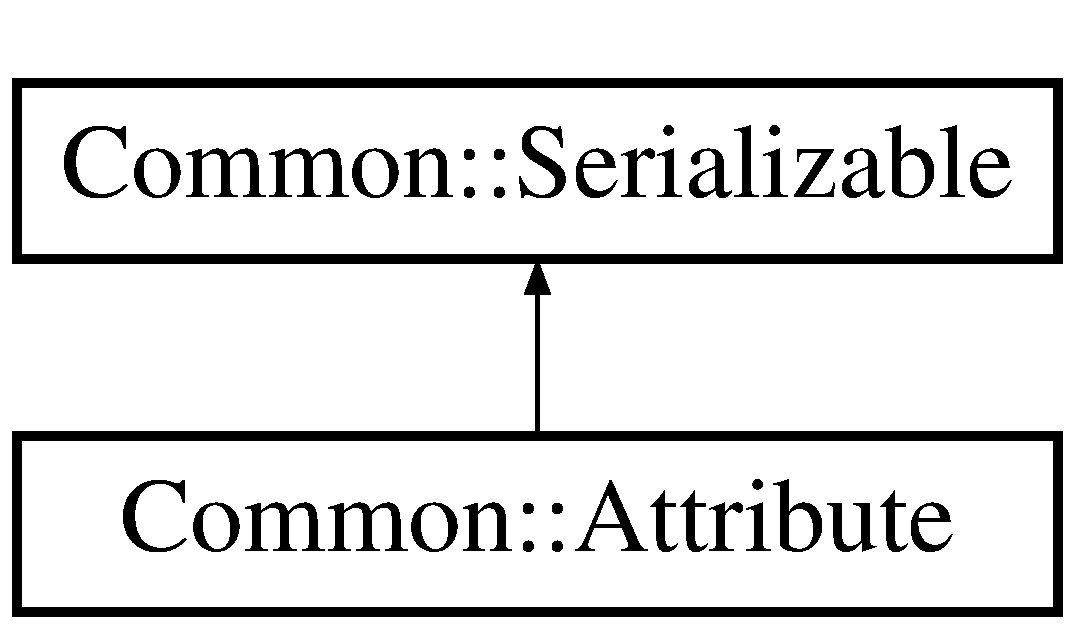
\includegraphics[height=2.000000cm]{class_common_1_1_attribute}
\end{center}
\end{figure}
\subsection*{Public Member Functions}
\begin{DoxyCompactItemize}
\item 
\hypertarget{class_common_1_1_attribute_a3ba016fa5cb64736d1d32fffda0df30d}{\hyperlink{class_common_1_1_attribute_a3ba016fa5cb64736d1d32fffda0df30d}{Attribute} (\hyperlink{class_common_1_1_attribute}{Attribute} const \&a)}\label{class_common_1_1_attribute_a3ba016fa5cb64736d1d32fffda0df30d}

\begin{DoxyCompactList}\small\item\em Copy constructor. \end{DoxyCompactList}\item 
\hyperlink{class_common_1_1_attribute_a9413ac7a553fa1b45db960aee7661bb1}{Attribute} ()
\begin{DoxyCompactList}\small\item\em Constructor. \end{DoxyCompactList}\item 
\hypertarget{class_common_1_1_attribute_a04e52cfb65fde9d7a1865889b766a252}{void \hyperlink{class_common_1_1_attribute_a04e52cfb65fde9d7a1865889b766a252}{Serialize} (\hyperlink{class_common_1_1_serializer}{Serializer} \&out) const }\label{class_common_1_1_attribute_a04e52cfb65fde9d7a1865889b766a252}

\begin{DoxyCompactList}\small\item\em Sends the data serialized. \end{DoxyCompactList}\item 
\hypertarget{class_common_1_1_attribute_ad29f02520158693684097d1d641ad663}{void \hyperlink{class_common_1_1_attribute_ad29f02520158693684097d1d641ad663}{De\-Serialize} (\hyperlink{class_common_1_1_de_serializer}{De\-Serializer} \&in)}\label{class_common_1_1_attribute_ad29f02520158693684097d1d641ad663}

\begin{DoxyCompactList}\small\item\em Gets the data deserialized. \end{DoxyCompactList}\item 
\hypertarget{class_common_1_1_attribute_ad186aab5840424763a5681a01dbda573}{string \hyperlink{class_common_1_1_attribute_ad186aab5840424763a5681a01dbda573}{Get\-Source\-String} () const }\label{class_common_1_1_attribute_ad186aab5840424763a5681a01dbda573}

\begin{DoxyCompactList}\small\item\em Returns the string of the source. \end{DoxyCompactList}\item 
\hypertarget{class_common_1_1_attribute_a0216c228ccddf6c48b263a7bf85a22f5}{string \hyperlink{class_common_1_1_attribute_a0216c228ccddf6c48b263a7bf85a22f5}{Get\-Type\-String} () const }\label{class_common_1_1_attribute_a0216c228ccddf6c48b263a7bf85a22f5}

\begin{DoxyCompactList}\small\item\em Returns the type of the attribute. \end{DoxyCompactList}\item 
\hypertarget{class_common_1_1_attribute_a2e324783d3f8c637ba014bb31f57a0f3}{void \hyperlink{class_common_1_1_attribute_a2e324783d3f8c637ba014bb31f57a0f3}{Dump} () const }\label{class_common_1_1_attribute_a2e324783d3f8c637ba014bb31f57a0f3}

\begin{DoxyCompactList}\small\item\em Logs the information of the attribute on the System Log. \end{DoxyCompactList}\end{DoxyCompactItemize}
\subsection*{Static Public Member Functions}
\begin{DoxyCompactItemize}
\item 
\hypertarget{class_common_1_1_attribute_a6eb5558c76b0ee62bda3316527a4efe1}{static string \hyperlink{class_common_1_1_attribute_a6eb5558c76b0ee62bda3316527a4efe1}{Get\-Type\-String} (Attr\-Value\-Type type)}\label{class_common_1_1_attribute_a6eb5558c76b0ee62bda3316527a4efe1}

\begin{DoxyCompactList}\small\item\em Given a value of the enumerator Attr\-Value\-Type returns the type in a string. \end{DoxyCompactList}\end{DoxyCompactItemize}
\subsection*{Public Attributes}
\begin{DoxyCompactItemize}
\item 
\hypertarget{class_common_1_1_attribute_a9c6c88466932374ae50f159b409accc5}{Attr\-Source {\bfseries source}}\label{class_common_1_1_attribute_a9c6c88466932374ae50f159b409accc5}

\item 
\hypertarget{class_common_1_1_attribute_acdf1e1cfa052178691bbb9c237395af5}{Attr\-Value\-Type {\bfseries type}}\label{class_common_1_1_attribute_acdf1e1cfa052178691bbb9c237395af5}

\item 
\hypertarget{class_common_1_1_attribute_aa8ba600fea107d6cea62233f8358b2f1}{string {\bfseries id}}\label{class_common_1_1_attribute_aa8ba600fea107d6cea62233f8358b2f1}

\end{DoxyCompactItemize}


\subsection{Detailed Description}
Contains the necessary information of an attribute to be inserted in a program. 

\begin{DoxyVersion}{Version}
1.\-0b 
\end{DoxyVersion}
\begin{DoxySince}{Since}
1.\-0b 
\end{DoxySince}
\begin{DoxyAuthor}{Author}
Ania Sikora, 2002 
\end{DoxyAuthor}


\subsection{Constructor \& Destructor Documentation}
\hypertarget{class_common_1_1_attribute_a9413ac7a553fa1b45db960aee7661bb1}{\index{Common\-::\-Attribute@{Common\-::\-Attribute}!Attribute@{Attribute}}
\index{Attribute@{Attribute}!Common::Attribute@{Common\-::\-Attribute}}
\subsubsection[{Attribute}]{\setlength{\rightskip}{0pt plus 5cm}Common\-::\-Attribute\-::\-Attribute (
\begin{DoxyParamCaption}
{}
\end{DoxyParamCaption}
)\hspace{0.3cm}{\ttfamily [inline]}}}\label{class_common_1_1_attribute_a9413ac7a553fa1b45db960aee7661bb1}


Constructor. 

Creates a default \hyperlink{class_common_1_1_attribute}{Attribute} object of the integer type. 

The documentation for this class was generated from the following files\-:\begin{DoxyCompactItemize}
\item 
Common/Utils.\-h\item 
Common/Utils.\-cpp\end{DoxyCompactItemize}

\hypertarget{class_common_1_1_attribute_value}{\section{Common\-:\-:Attribute\-Value Class Reference}
\label{class_common_1_1_attribute_value}\index{Common\-::\-Attribute\-Value@{Common\-::\-Attribute\-Value}}
}


Contains the vale of an attribute.  




{\ttfamily \#include $<$Utils.\-h$>$}

Inheritance diagram for Common\-:\-:Attribute\-Value\-:\begin{figure}[H]
\begin{center}
\leavevmode
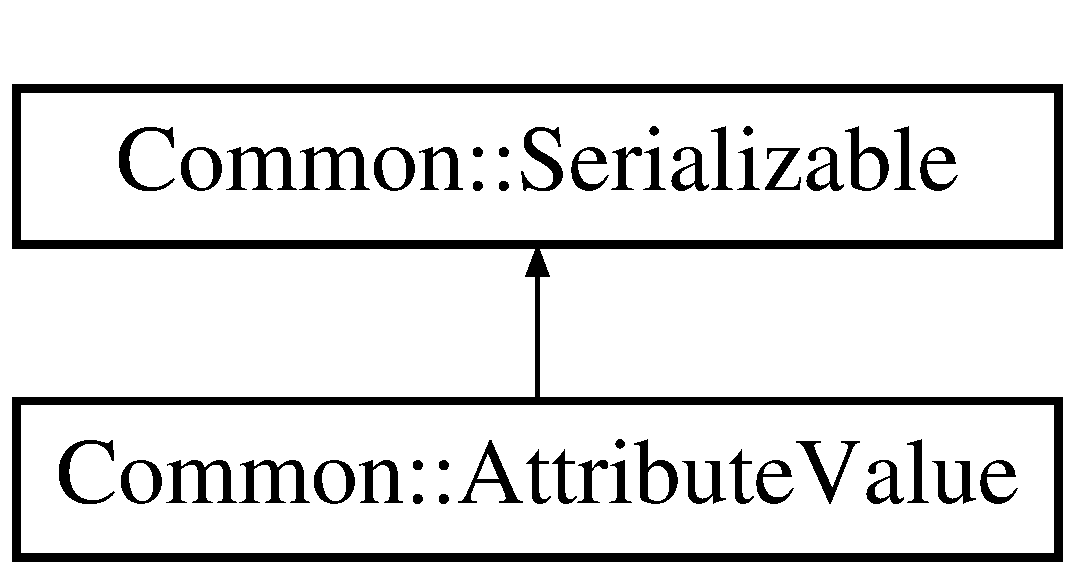
\includegraphics[height=2.000000cm]{class_common_1_1_attribute_value}
\end{center}
\end{figure}
\subsection*{Public Member Functions}
\begin{DoxyCompactItemize}
\item 
\hypertarget{class_common_1_1_attribute_value_a85fc10d30887464438324f511e415e04}{\hyperlink{class_common_1_1_attribute_value_a85fc10d30887464438324f511e415e04}{Attribute\-Value} ()}\label{class_common_1_1_attribute_value_a85fc10d30887464438324f511e415e04}

\begin{DoxyCompactList}\small\item\em Constructor. \end{DoxyCompactList}\item 
\hypertarget{class_common_1_1_attribute_value_aca5adecb66fd562acd287986fd52e78d}{\hyperlink{class_common_1_1_attribute_value_aca5adecb66fd562acd287986fd52e78d}{Attribute\-Value} (\hyperlink{class_common_1_1_attribute_value}{Attribute\-Value} const \&av)}\label{class_common_1_1_attribute_value_aca5adecb66fd562acd287986fd52e78d}

\begin{DoxyCompactList}\small\item\em Copy constructor. \end{DoxyCompactList}\item 
\hypertarget{class_common_1_1_attribute_value_acc398a13933363ebf35f0871fa70ed53}{void \hyperlink{class_common_1_1_attribute_value_acc398a13933363ebf35f0871fa70ed53}{operator=} (\hyperlink{class_common_1_1_attribute_value}{Attribute\-Value} const \&av)}\label{class_common_1_1_attribute_value_acc398a13933363ebf35f0871fa70ed53}

\begin{DoxyCompactList}\small\item\em Assignation operator, copies content of the given object. \end{DoxyCompactList}\item 
\hypertarget{class_common_1_1_attribute_value_a5a1f75aa6614c5c66e068d4e504c5811}{Attr\-Value\-Type \hyperlink{class_common_1_1_attribute_value_a5a1f75aa6614c5c66e068d4e504c5811}{Get\-Type} () const }\label{class_common_1_1_attribute_value_a5a1f75aa6614c5c66e068d4e504c5811}

\begin{DoxyCompactList}\small\item\em Returns type of the attribute. \end{DoxyCompactList}\item 
\hypertarget{class_common_1_1_attribute_value_a0891619e861ce488d2633479c60513e7}{void \hyperlink{class_common_1_1_attribute_value_a0891619e861ce488d2633479c60513e7}{Set\-Type} (Attr\-Value\-Type attr\-Type)}\label{class_common_1_1_attribute_value_a0891619e861ce488d2633479c60513e7}

\begin{DoxyCompactList}\small\item\em Sets the type of the attribute. \end{DoxyCompactList}\item 
\hypertarget{class_common_1_1_attribute_value_a8490303562e2b91c85bdfed728be133b}{void \hyperlink{class_common_1_1_attribute_value_a8490303562e2b91c85bdfed728be133b}{Set\-Str\-Value} (std\-::string attr\-Str\-Value)}\label{class_common_1_1_attribute_value_a8490303562e2b91c85bdfed728be133b}

\begin{DoxyCompactList}\small\item\em Sets the string value of the attribute. \end{DoxyCompactList}\item 
int \hyperlink{class_common_1_1_attribute_value_a87062c697e4a89b885fa24d129e7aff6}{Get\-Int\-Value} () const 
\begin{DoxyCompactList}\small\item\em Gets the integer value. \end{DoxyCompactList}\item 
std\-::string \hyperlink{class_common_1_1_attribute_value_ad7996923bcce2668a865b59b00bfc51e}{Get\-String\-Value} () const 
\begin{DoxyCompactList}\small\item\em Gets the string value. \end{DoxyCompactList}\item 
short \hyperlink{class_common_1_1_attribute_value_acd0a3ae4799eb19c3e1d874f0c9c16c8}{Get\-Short\-Value} () const 
\begin{DoxyCompactList}\small\item\em Gets the short value. \end{DoxyCompactList}\item 
float \hyperlink{class_common_1_1_attribute_value_a5c9d419b404347da61c975f1a551ddac}{Get\-Float\-Value} () const 
\begin{DoxyCompactList}\small\item\em Gets the float value. \end{DoxyCompactList}\item 
double \hyperlink{class_common_1_1_attribute_value_af6955bdc86e6b448d5b578c0855c20c9}{Get\-Double\-Value} () const 
\begin{DoxyCompactList}\small\item\em Gets the double value. \end{DoxyCompactList}\item 
char \hyperlink{class_common_1_1_attribute_value_a8fb7b23d3590bbd68cdbdbc47b7f81c1}{Get\-Char\-Value} () const 
\begin{DoxyCompactList}\small\item\em Gets the char value. \end{DoxyCompactList}\item 
\hypertarget{class_common_1_1_attribute_value_ad2582a6c83ae1e37355848fed70838c4}{void $\ast$ \hyperlink{class_common_1_1_attribute_value_ad2582a6c83ae1e37355848fed70838c4}{Get\-Value\-Buffer} ()}\label{class_common_1_1_attribute_value_ad2582a6c83ae1e37355848fed70838c4}

\begin{DoxyCompactList}\small\item\em Gets the pointer to the buffer. \end{DoxyCompactList}\item 
\hypertarget{class_common_1_1_attribute_value_a3435da1e6c57b584ee29bc8a049f0238}{int \hyperlink{class_common_1_1_attribute_value_a3435da1e6c57b584ee29bc8a049f0238}{Get\-Size} () const }\label{class_common_1_1_attribute_value_a3435da1e6c57b584ee29bc8a049f0238}

\begin{DoxyCompactList}\small\item\em Gets the size of the value in memory. \end{DoxyCompactList}\item 
\hypertarget{class_common_1_1_attribute_value_ac1e6e84769713f29fd4fb88a90d37bc0}{string \hyperlink{class_common_1_1_attribute_value_ac1e6e84769713f29fd4fb88a90d37bc0}{To\-String} () const }\label{class_common_1_1_attribute_value_ac1e6e84769713f29fd4fb88a90d37bc0}

\begin{DoxyCompactList}\small\item\em Returns the value in a string. \end{DoxyCompactList}\item 
\hypertarget{class_common_1_1_attribute_value_ade3586150d8f58331f56de64e8221088}{void \hyperlink{class_common_1_1_attribute_value_ade3586150d8f58331f56de64e8221088}{Serialize} (\hyperlink{class_common_1_1_serializer}{Serializer} \&out) const }\label{class_common_1_1_attribute_value_ade3586150d8f58331f56de64e8221088}

\begin{DoxyCompactList}\small\item\em Sends the data serialized. \end{DoxyCompactList}\item 
\hypertarget{class_common_1_1_attribute_value_a71ef76a176138452c6a5ba8a00d42502}{void \hyperlink{class_common_1_1_attribute_value_a71ef76a176138452c6a5ba8a00d42502}{De\-Serialize} (\hyperlink{class_common_1_1_de_serializer}{De\-Serializer} \&in)}\label{class_common_1_1_attribute_value_a71ef76a176138452c6a5ba8a00d42502}

\begin{DoxyCompactList}\small\item\em Gets the data deserialized. \end{DoxyCompactList}\end{DoxyCompactItemize}
\subsection*{Public Attributes}
\begin{DoxyCompactItemize}
\item 
\hypertarget{class_common_1_1_attribute_value_a1f23a57622ee2685e0dd3da74e3ad8e9}{\begin{tabbing}
xx\=xx\=xx\=xx\=xx\=xx\=xx\=xx\=xx\=\kill
union \{\\
\>int {\bfseries intValue}\\
\>short {\bfseries shortValue}\\
\>float {\bfseries floatValue}\\
\>double {\bfseries doubleValue}\\
\>char {\bfseries charValue}\\
\}; }\label{class_common_1_1_attribute_value_a1f23a57622ee2685e0dd3da74e3ad8e9}
\\

\end{tabbing}\end{DoxyCompactItemize}


\subsection{Detailed Description}
Contains the vale of an attribute. 

\begin{DoxyVersion}{Version}
1.\-0b 
\end{DoxyVersion}
\begin{DoxySince}{Since}
1.\-0b 
\end{DoxySince}
\begin{DoxyAuthor}{Author}
Ania Sikora, 2002 
\end{DoxyAuthor}


\subsection{Member Function Documentation}
\hypertarget{class_common_1_1_attribute_value_a8fb7b23d3590bbd68cdbdbc47b7f81c1}{\index{Common\-::\-Attribute\-Value@{Common\-::\-Attribute\-Value}!Get\-Char\-Value@{Get\-Char\-Value}}
\index{Get\-Char\-Value@{Get\-Char\-Value}!Common::AttributeValue@{Common\-::\-Attribute\-Value}}
\subsubsection[{Get\-Char\-Value}]{\setlength{\rightskip}{0pt plus 5cm}char Attribute\-Value\-::\-Get\-Char\-Value (
\begin{DoxyParamCaption}
{}
\end{DoxyParamCaption}
) const\hspace{0.3cm}{\ttfamily [inline]}}}\label{class_common_1_1_attribute_value_a8fb7b23d3590bbd68cdbdbc47b7f81c1}


Gets the char value. 


\begin{DoxyExceptions}{Exceptions}
{\em \hyperlink{class_common_1_1_exception}{Exception}} & \\
\hline
\end{DoxyExceptions}
\hypertarget{class_common_1_1_attribute_value_af6955bdc86e6b448d5b578c0855c20c9}{\index{Common\-::\-Attribute\-Value@{Common\-::\-Attribute\-Value}!Get\-Double\-Value@{Get\-Double\-Value}}
\index{Get\-Double\-Value@{Get\-Double\-Value}!Common::AttributeValue@{Common\-::\-Attribute\-Value}}
\subsubsection[{Get\-Double\-Value}]{\setlength{\rightskip}{0pt plus 5cm}double Attribute\-Value\-::\-Get\-Double\-Value (
\begin{DoxyParamCaption}
{}
\end{DoxyParamCaption}
) const\hspace{0.3cm}{\ttfamily [inline]}}}\label{class_common_1_1_attribute_value_af6955bdc86e6b448d5b578c0855c20c9}


Gets the double value. 


\begin{DoxyExceptions}{Exceptions}
{\em \hyperlink{class_common_1_1_exception}{Exception}} & \\
\hline
\end{DoxyExceptions}
\hypertarget{class_common_1_1_attribute_value_a5c9d419b404347da61c975f1a551ddac}{\index{Common\-::\-Attribute\-Value@{Common\-::\-Attribute\-Value}!Get\-Float\-Value@{Get\-Float\-Value}}
\index{Get\-Float\-Value@{Get\-Float\-Value}!Common::AttributeValue@{Common\-::\-Attribute\-Value}}
\subsubsection[{Get\-Float\-Value}]{\setlength{\rightskip}{0pt plus 5cm}float Attribute\-Value\-::\-Get\-Float\-Value (
\begin{DoxyParamCaption}
{}
\end{DoxyParamCaption}
) const\hspace{0.3cm}{\ttfamily [inline]}}}\label{class_common_1_1_attribute_value_a5c9d419b404347da61c975f1a551ddac}


Gets the float value. 


\begin{DoxyExceptions}{Exceptions}
{\em \hyperlink{class_common_1_1_exception}{Exception}} & \\
\hline
\end{DoxyExceptions}
\hypertarget{class_common_1_1_attribute_value_a87062c697e4a89b885fa24d129e7aff6}{\index{Common\-::\-Attribute\-Value@{Common\-::\-Attribute\-Value}!Get\-Int\-Value@{Get\-Int\-Value}}
\index{Get\-Int\-Value@{Get\-Int\-Value}!Common::AttributeValue@{Common\-::\-Attribute\-Value}}
\subsubsection[{Get\-Int\-Value}]{\setlength{\rightskip}{0pt plus 5cm}int Attribute\-Value\-::\-Get\-Int\-Value (
\begin{DoxyParamCaption}
{}
\end{DoxyParamCaption}
) const\hspace{0.3cm}{\ttfamily [inline]}}}\label{class_common_1_1_attribute_value_a87062c697e4a89b885fa24d129e7aff6}


Gets the integer value. 


\begin{DoxyExceptions}{Exceptions}
{\em \hyperlink{class_common_1_1_exception}{Exception}} & \\
\hline
\end{DoxyExceptions}
\hypertarget{class_common_1_1_attribute_value_acd0a3ae4799eb19c3e1d874f0c9c16c8}{\index{Common\-::\-Attribute\-Value@{Common\-::\-Attribute\-Value}!Get\-Short\-Value@{Get\-Short\-Value}}
\index{Get\-Short\-Value@{Get\-Short\-Value}!Common::AttributeValue@{Common\-::\-Attribute\-Value}}
\subsubsection[{Get\-Short\-Value}]{\setlength{\rightskip}{0pt plus 5cm}short Attribute\-Value\-::\-Get\-Short\-Value (
\begin{DoxyParamCaption}
{}
\end{DoxyParamCaption}
) const\hspace{0.3cm}{\ttfamily [inline]}}}\label{class_common_1_1_attribute_value_acd0a3ae4799eb19c3e1d874f0c9c16c8}


Gets the short value. 


\begin{DoxyExceptions}{Exceptions}
{\em \hyperlink{class_common_1_1_exception}{Exception}} & \\
\hline
\end{DoxyExceptions}
\hypertarget{class_common_1_1_attribute_value_ad7996923bcce2668a865b59b00bfc51e}{\index{Common\-::\-Attribute\-Value@{Common\-::\-Attribute\-Value}!Get\-String\-Value@{Get\-String\-Value}}
\index{Get\-String\-Value@{Get\-String\-Value}!Common::AttributeValue@{Common\-::\-Attribute\-Value}}
\subsubsection[{Get\-String\-Value}]{\setlength{\rightskip}{0pt plus 5cm}std\-::string Attribute\-Value\-::\-Get\-String\-Value (
\begin{DoxyParamCaption}
{}
\end{DoxyParamCaption}
) const\hspace{0.3cm}{\ttfamily [inline]}}}\label{class_common_1_1_attribute_value_ad7996923bcce2668a865b59b00bfc51e}


Gets the string value. 


\begin{DoxyExceptions}{Exceptions}
{\em \hyperlink{class_common_1_1_exception}{Exception}} & \\
\hline
\end{DoxyExceptions}


The documentation for this class was generated from the following files\-:\begin{DoxyCompactItemize}
\item 
Common/Utils.\-h\item 
Common/Utils.\-cpp\end{DoxyCompactItemize}

\hypertarget{classauto__iterator}{\section{auto\-\_\-iterator$<$ T $>$ Class Template Reference}
\label{classauto__iterator}\index{auto\-\_\-iterator$<$ T $>$@{auto\-\_\-iterator$<$ T $>$}}
}


Class that implements the {\itshape auto\-\_\-ptrs} operators.  




{\ttfamily \#include $<$auto\-\_\-vector.\-h$>$}

\subsection*{Public Member Functions}
\begin{DoxyCompactItemize}
\item 
\hypertarget{classauto__iterator_aebfd2b8221b5003ff09946b6e7058481}{{\bfseries auto\-\_\-iterator} (auto\-\_\-ptr$<$ T $>$ $\ast$pp)}\label{classauto__iterator_aebfd2b8221b5003ff09946b6e7058481}

\item 
\hypertarget{classauto__iterator_acaf821dd51def74ccfea7df4303a5844}{bool {\bfseries operator!=} (\hyperlink{classauto__iterator}{auto\-\_\-iterator}$<$ T $>$ const \&it) const }\label{classauto__iterator_acaf821dd51def74ccfea7df4303a5844}

\item 
\hypertarget{classauto__iterator_a25da7c273f44b6874b0aa688b51a0324}{\hyperlink{classauto__iterator}{auto\-\_\-iterator} const \& {\bfseries operator++} (int)}\label{classauto__iterator_a25da7c273f44b6874b0aa688b51a0324}

\item 
\hypertarget{classauto__iterator_aaead03d74bac44a44742bd6dd80a39a8}{\hyperlink{classauto__iterator}{auto\-\_\-iterator} {\bfseries operator++} ()}\label{classauto__iterator_aaead03d74bac44a44742bd6dd80a39a8}

\item 
\hypertarget{classauto__iterator_a4d3bbf29747a8e078ccbb348e1ca5405}{T $\ast$ {\bfseries operator$\ast$} ()}\label{classauto__iterator_a4d3bbf29747a8e078ccbb348e1ca5405}

\item 
\hypertarget{classauto__iterator_a0009eb5d3cee4489204e8f0cde9f9157}{T const $\ast$ {\bfseries operator$\ast$} () const }\label{classauto__iterator_a0009eb5d3cee4489204e8f0cde9f9157}

\item 
\hypertarget{classauto__iterator_ae97c529538345fea66485049e7e4667f}{T $\ast$ {\bfseries operator-\/$>$} ()}\label{classauto__iterator_ae97c529538345fea66485049e7e4667f}

\end{DoxyCompactItemize}


\subsection{Detailed Description}
\subsubsection*{template$<$class T$>$class auto\-\_\-iterator$<$ T $>$}

Class that implements the {\itshape auto\-\_\-ptrs} operators. 

\begin{DoxyVersion}{Version}
1.\-0b 
\end{DoxyVersion}
\begin{DoxyAuthor}{Author}
Ania Sikora, 2002 
\end{DoxyAuthor}
\begin{DoxySince}{Since}
1.\-0b 
\end{DoxySince}


The documentation for this class was generated from the following file\-:\begin{DoxyCompactItemize}
\item 
Common/auto\-\_\-vector.\-h\end{DoxyCompactItemize}

\hypertarget{classauto__vector}{\section{auto\-\_\-vector$<$ T $>$ Class Template Reference}
\label{classauto__vector}\index{auto\-\_\-vector$<$ T $>$@{auto\-\_\-vector$<$ T $>$}}
}


Class with the methods to create, handle and destroy an array of {\itshape auto\-\_\-ptr} elements.  




{\ttfamily \#include $<$auto\-\_\-vector.\-h$>$}

\subsection*{Public Types}
\begin{DoxyCompactItemize}
\item 
\hypertarget{classauto__vector_a0851c5a49cd4b8b5e5bc9d1319c53c9e}{typedef \hyperlink{classauto__iterator}{auto\-\_\-iterator}$<$ T $>$ {\bfseries iterator}}\label{classauto__vector_a0851c5a49cd4b8b5e5bc9d1319c53c9e}

\end{DoxyCompactItemize}
\subsection*{Public Member Functions}
\begin{DoxyCompactItemize}
\item 
\hyperlink{classauto__vector_ab463df1a0a9c3f3cb6943b33e3ef8e50}{auto\-\_\-vector} (size\-\_\-t capacity=0)
\begin{DoxyCompactList}\small\item\em Constructor. \end{DoxyCompactList}\item 
\hypertarget{classauto__vector_a7858fbbe2f4d94be3df80d48f4862f3c}{\hyperlink{classauto__vector_a7858fbbe2f4d94be3df80d48f4862f3c}{$\sim$auto\-\_\-vector} ()}\label{classauto__vector_a7858fbbe2f4d94be3df80d48f4862f3c}

\begin{DoxyCompactList}\small\item\em Destructor. \end{DoxyCompactList}\item 
\hypertarget{classauto__vector_a3be25f0b235aae9b7f4d11fbd0388eee}{T const $\ast$ {\bfseries operator\mbox{[}$\,$\mbox{]}} (size\-\_\-t i) const }\label{classauto__vector_a3be25f0b235aae9b7f4d11fbd0388eee}

\item 
\hypertarget{classauto__vector_ad8d0dc748236e2a49675918e114c9bf1}{T $\ast$ {\bfseries operator\mbox{[}$\,$\mbox{]}} (size\-\_\-t i)}\label{classauto__vector_ad8d0dc748236e2a49675918e114c9bf1}

\item 
void \hyperlink{classauto__vector_aaa9c829b0a79ba7b04c6d670a0b4560c}{assign} (size\-\_\-t i, auto\-\_\-ptr$<$ T $>$ \&p)
\begin{DoxyCompactList}\small\item\em Assigns {\itshape p} to the {\itshape ith} position in the \hyperlink{classauto__vector}{auto\-\_\-vector} array \-\_\-arr. \end{DoxyCompactList}\item 
void \hyperlink{classauto__vector_ae912e8d33747dd0bd1dac1bd6253739d}{remove\-\_\-direct} (size\-\_\-t i, T $\ast$p)
\begin{DoxyCompactList}\small\item\em Deletes position {\itshape i} in the array. \end{DoxyCompactList}\item 
\hypertarget{classauto__vector_ac84a439202d7e6a8a7455b6bd9007f67}{void \hyperlink{classauto__vector_ac84a439202d7e6a8a7455b6bd9007f67}{Dump} ()}\label{classauto__vector_ac84a439202d7e6a8a7455b6bd9007f67}

\begin{DoxyCompactList}\small\item\em Prints the contents in the \hyperlink{classauto__vector}{auto\-\_\-vector} array \-\_\-arr. \end{DoxyCompactList}\item 
\hypertarget{classauto__vector_a764809bfe8ea1bce8f0bde7c79839ba3}{void \hyperlink{classauto__vector_a764809bfe8ea1bce8f0bde7c79839ba3}{clear} ()}\label{classauto__vector_a764809bfe8ea1bce8f0bde7c79839ba3}

\begin{DoxyCompactList}\small\item\em Deletes all contents in the \hyperlink{classauto__vector}{auto\-\_\-vector} array \-\_\-arr. \end{DoxyCompactList}\item 
void \hyperlink{classauto__vector_a0495393c94517c0a25af3f00f9afb845}{push\-\_\-back} (auto\-\_\-ptr$<$ T $>$ \&p)
\begin{DoxyCompactList}\small\item\em Pushes an element {\itshape p} at the end of the \hyperlink{classauto__vector}{auto\-\_\-vector} array \-\_\-arr. \end{DoxyCompactList}\item 
auto\-\_\-ptr$<$ T $>$ \hyperlink{classauto__vector_a4d6b60c1b38d1c8bbe9c9dc808743f29}{pop\-\_\-back} ()
\begin{DoxyCompactList}\small\item\em Pops the last element of the \hyperlink{classauto__vector}{auto\-\_\-vector} array \-\_\-arr. \end{DoxyCompactList}\item 
auto\-\_\-ptr$<$ T $>$ \hyperlink{classauto__vector_a53de704658c049839e5e75da35b14602}{acquire} (size\-\_\-t i)
\begin{DoxyCompactList}\small\item\em Gets the contents from vector \-\_\-arr in the given position. \end{DoxyCompactList}\item 
\hyperlink{classauto__iterator}{iterator} \hyperlink{classauto__vector_a0690df2f134d5e8318508fe2f00ed7fd}{begin} () const 
\begin{DoxyCompactList}\small\item\em Returns a pointer to the first position in the array \-\_\-arr. \end{DoxyCompactList}\item 
\hyperlink{classauto__iterator}{iterator} \hyperlink{classauto__vector_a266e4fb18cbd0af7d685c97ddf18100d}{end} () const 
\begin{DoxyCompactList}\small\item\em Returns a pointer to the last position in the array \-\_\-arr. \end{DoxyCompactList}\item 
int \hyperlink{classauto__vector_a5cac8d686d7fd1ae675932737661607a}{size} () const 
\begin{DoxyCompactList}\small\item\em Returns the size of \-\_\-arr. \end{DoxyCompactList}\end{DoxyCompactItemize}


\subsection{Detailed Description}
\subsubsection*{template$<$class T$>$class auto\-\_\-vector$<$ T $>$}

Class with the methods to create, handle and destroy an array of {\itshape auto\-\_\-ptr} elements. 

\begin{DoxyVersion}{Version}
1.\-0b 
\end{DoxyVersion}
\begin{DoxyAuthor}{Author}
Ania Sikora, 2002 
\end{DoxyAuthor}
\begin{DoxySince}{Since}
1.\-0b 
\end{DoxySince}


\subsection{Constructor \& Destructor Documentation}
\hypertarget{classauto__vector_ab463df1a0a9c3f3cb6943b33e3ef8e50}{\index{auto\-\_\-vector@{auto\-\_\-vector}!auto\-\_\-vector@{auto\-\_\-vector}}
\index{auto\-\_\-vector@{auto\-\_\-vector}!auto_vector@{auto\-\_\-vector}}
\subsubsection[{auto\-\_\-vector}]{\setlength{\rightskip}{0pt plus 5cm}template$<$class T$>$ {\bf auto\-\_\-vector}$<$ T $>$\-::{\bf auto\-\_\-vector} (
\begin{DoxyParamCaption}
\item[{size\-\_\-t}]{capacity = {\ttfamily 0}}
\end{DoxyParamCaption}
)\hspace{0.3cm}{\ttfamily [inline]}, {\ttfamily [explicit]}}}\label{classauto__vector_ab463df1a0a9c3f3cb6943b33e3ef8e50}


Constructor. 


\begin{DoxyParams}{Parameters}
{\em capacity} & Vector capacity. By default this is 0 \\
\hline
\end{DoxyParams}


\subsection{Member Function Documentation}
\hypertarget{classauto__vector_a53de704658c049839e5e75da35b14602}{\index{auto\-\_\-vector@{auto\-\_\-vector}!acquire@{acquire}}
\index{acquire@{acquire}!auto_vector@{auto\-\_\-vector}}
\subsubsection[{acquire}]{\setlength{\rightskip}{0pt plus 5cm}template$<$class T$>$ auto\-\_\-ptr$<$T$>$ {\bf auto\-\_\-vector}$<$ T $>$\-::acquire (
\begin{DoxyParamCaption}
\item[{size\-\_\-t}]{i}
\end{DoxyParamCaption}
)\hspace{0.3cm}{\ttfamily [inline]}}}\label{classauto__vector_a53de704658c049839e5e75da35b14602}


Gets the contents from vector \-\_\-arr in the given position. 


\begin{DoxyParams}{Parameters}
{\em i} & Position of the element we want to get from \-\_\-arr \\
\hline
\end{DoxyParams}
\begin{DoxyReturn}{Returns}
Contents of the {\itshape ith} element in \-\_\-arr 
\end{DoxyReturn}
\hypertarget{classauto__vector_aaa9c829b0a79ba7b04c6d670a0b4560c}{\index{auto\-\_\-vector@{auto\-\_\-vector}!assign@{assign}}
\index{assign@{assign}!auto_vector@{auto\-\_\-vector}}
\subsubsection[{assign}]{\setlength{\rightskip}{0pt plus 5cm}template$<$class T$>$ void {\bf auto\-\_\-vector}$<$ T $>$\-::assign (
\begin{DoxyParamCaption}
\item[{size\-\_\-t}]{i, }
\item[{auto\-\_\-ptr$<$ T $>$ \&}]{p}
\end{DoxyParamCaption}
)\hspace{0.3cm}{\ttfamily [inline]}}}\label{classauto__vector_aaa9c829b0a79ba7b04c6d670a0b4560c}


Assigns {\itshape p} to the {\itshape ith} position in the \hyperlink{classauto__vector}{auto\-\_\-vector} array \-\_\-arr. 


\begin{DoxyParams}{Parameters}
{\em i} & Position where to make the assignment \\
\hline
{\em p} & Data that will be assigned \\
\hline
\end{DoxyParams}
\hypertarget{classauto__vector_a0690df2f134d5e8318508fe2f00ed7fd}{\index{auto\-\_\-vector@{auto\-\_\-vector}!begin@{begin}}
\index{begin@{begin}!auto_vector@{auto\-\_\-vector}}
\subsubsection[{begin}]{\setlength{\rightskip}{0pt plus 5cm}template$<$class T$>$ {\bf iterator} {\bf auto\-\_\-vector}$<$ T $>$\-::begin (
\begin{DoxyParamCaption}
{}
\end{DoxyParamCaption}
) const\hspace{0.3cm}{\ttfamily [inline]}}}\label{classauto__vector_a0690df2f134d5e8318508fe2f00ed7fd}


Returns a pointer to the first position in the array \-\_\-arr. 

\begin{DoxyReturn}{Returns}
First position in \-\_\-arr 
\end{DoxyReturn}
\hypertarget{classauto__vector_a266e4fb18cbd0af7d685c97ddf18100d}{\index{auto\-\_\-vector@{auto\-\_\-vector}!end@{end}}
\index{end@{end}!auto_vector@{auto\-\_\-vector}}
\subsubsection[{end}]{\setlength{\rightskip}{0pt plus 5cm}template$<$class T$>$ {\bf iterator} {\bf auto\-\_\-vector}$<$ T $>$\-::end (
\begin{DoxyParamCaption}
{}
\end{DoxyParamCaption}
) const\hspace{0.3cm}{\ttfamily [inline]}}}\label{classauto__vector_a266e4fb18cbd0af7d685c97ddf18100d}


Returns a pointer to the last position in the array \-\_\-arr. 

\begin{DoxyReturn}{Returns}
Ending position in \-\_\-arr 
\end{DoxyReturn}
\hypertarget{classauto__vector_a4d6b60c1b38d1c8bbe9c9dc808743f29}{\index{auto\-\_\-vector@{auto\-\_\-vector}!pop\-\_\-back@{pop\-\_\-back}}
\index{pop\-\_\-back@{pop\-\_\-back}!auto_vector@{auto\-\_\-vector}}
\subsubsection[{pop\-\_\-back}]{\setlength{\rightskip}{0pt plus 5cm}template$<$class T$>$ auto\-\_\-ptr$<$T$>$ {\bf auto\-\_\-vector}$<$ T $>$\-::pop\-\_\-back (
\begin{DoxyParamCaption}
{}
\end{DoxyParamCaption}
)\hspace{0.3cm}{\ttfamily [inline]}}}\label{classauto__vector_a4d6b60c1b38d1c8bbe9c9dc808743f29}


Pops the last element of the \hyperlink{classauto__vector}{auto\-\_\-vector} array \-\_\-arr. 

\begin{DoxyReturn}{Returns}
Last element in \-\_\-arr 
\end{DoxyReturn}
\hypertarget{classauto__vector_a0495393c94517c0a25af3f00f9afb845}{\index{auto\-\_\-vector@{auto\-\_\-vector}!push\-\_\-back@{push\-\_\-back}}
\index{push\-\_\-back@{push\-\_\-back}!auto_vector@{auto\-\_\-vector}}
\subsubsection[{push\-\_\-back}]{\setlength{\rightskip}{0pt plus 5cm}template$<$class T$>$ void {\bf auto\-\_\-vector}$<$ T $>$\-::push\-\_\-back (
\begin{DoxyParamCaption}
\item[{auto\-\_\-ptr$<$ T $>$ \&}]{p}
\end{DoxyParamCaption}
)\hspace{0.3cm}{\ttfamily [inline]}}}\label{classauto__vector_a0495393c94517c0a25af3f00f9afb845}


Pushes an element {\itshape p} at the end of the \hyperlink{classauto__vector}{auto\-\_\-vector} array \-\_\-arr. 


\begin{DoxyParams}{Parameters}
{\em p} & \\
\hline
\end{DoxyParams}
\hypertarget{classauto__vector_ae912e8d33747dd0bd1dac1bd6253739d}{\index{auto\-\_\-vector@{auto\-\_\-vector}!remove\-\_\-direct@{remove\-\_\-direct}}
\index{remove\-\_\-direct@{remove\-\_\-direct}!auto_vector@{auto\-\_\-vector}}
\subsubsection[{remove\-\_\-direct}]{\setlength{\rightskip}{0pt plus 5cm}template$<$class T$>$ void {\bf auto\-\_\-vector}$<$ T $>$\-::remove\-\_\-direct (
\begin{DoxyParamCaption}
\item[{size\-\_\-t}]{i, }
\item[{T $\ast$}]{p}
\end{DoxyParamCaption}
)\hspace{0.3cm}{\ttfamily [inline]}}}\label{classauto__vector_ae912e8d33747dd0bd1dac1bd6253739d}


Deletes position {\itshape i} in the array. 


\begin{DoxyParams}{Parameters}
{\em i} & \\
\hline
{\em p} & \\
\hline
\end{DoxyParams}
\hypertarget{classauto__vector_a5cac8d686d7fd1ae675932737661607a}{\index{auto\-\_\-vector@{auto\-\_\-vector}!size@{size}}
\index{size@{size}!auto_vector@{auto\-\_\-vector}}
\subsubsection[{size}]{\setlength{\rightskip}{0pt plus 5cm}template$<$class T$>$ int {\bf auto\-\_\-vector}$<$ T $>$\-::size (
\begin{DoxyParamCaption}
{}
\end{DoxyParamCaption}
) const\hspace{0.3cm}{\ttfamily [inline]}}}\label{classauto__vector_a5cac8d686d7fd1ae675932737661607a}


Returns the size of \-\_\-arr. 

\begin{DoxyReturn}{Returns}
Number of elements in \-\_\-arr 
\end{DoxyReturn}


The documentation for this class was generated from the following file\-:\begin{DoxyCompactItemize}
\item 
Common/auto\-\_\-vector.\-h\end{DoxyCompactItemize}

\hypertarget{class_common_1_1_basic_log_filter}{\section{Common\-:\-:Basic\-Log\-Filter Class Reference}
\label{class_common_1_1_basic_log_filter}\index{Common\-::\-Basic\-Log\-Filter@{Common\-::\-Basic\-Log\-Filter}}
}


Filters \hyperlink{class_common_1_1_log_entry}{Log\-Entry} objects to be inserted in a log.  




{\ttfamily \#include $<$Syslog.\-h$>$}

Inheritance diagram for Common\-:\-:Basic\-Log\-Filter\-:\begin{figure}[H]
\begin{center}
\leavevmode
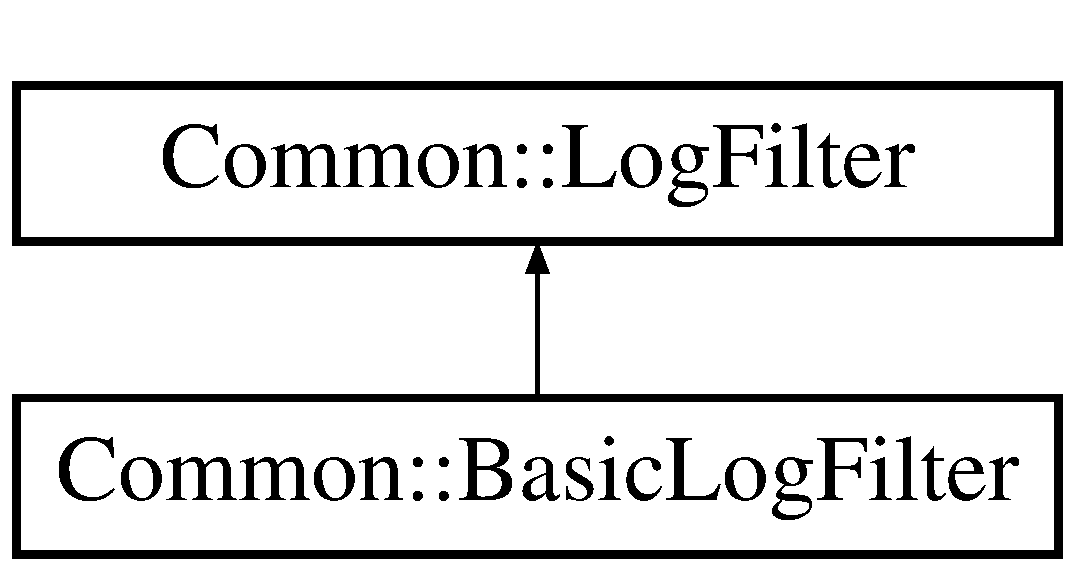
\includegraphics[height=2.000000cm]{class_common_1_1_basic_log_filter}
\end{center}
\end{figure}
\subsection*{Public Member Functions}
\begin{DoxyCompactItemize}
\item 
\hypertarget{class_common_1_1_basic_log_filter_a3c4f7c45a78fe892154822d2d48bb179}{\hyperlink{class_common_1_1_basic_log_filter_a3c4f7c45a78fe892154822d2d48bb179}{Basic\-Log\-Filter} ()}\label{class_common_1_1_basic_log_filter_a3c4f7c45a78fe892154822d2d48bb179}

\begin{DoxyCompactList}\small\item\em Constructor. \end{DoxyCompactList}\item 
\hyperlink{class_common_1_1_basic_log_filter_a5cfd74a2b7b89eb164f75a9db91cb1c2}{Basic\-Log\-Filter} (int mask)
\begin{DoxyCompactList}\small\item\em Constructor. \end{DoxyCompactList}\item 
\hypertarget{class_common_1_1_basic_log_filter_a6dcb632906cd269b32a659633060b008}{bool \hyperlink{class_common_1_1_basic_log_filter_a6dcb632906cd269b32a659633060b008}{Accept} (\hyperlink{class_common_1_1_log_entry}{Log\-Entry} const \&entry) const }\label{class_common_1_1_basic_log_filter_a6dcb632906cd269b32a659633060b008}

\begin{DoxyCompactList}\small\item\em Returns true if the log is accepted, false otherwise. \end{DoxyCompactList}\end{DoxyCompactItemize}


\subsection{Detailed Description}
Filters \hyperlink{class_common_1_1_log_entry}{Log\-Entry} objects to be inserted in a log. 

\begin{DoxyVersion}{Version}
1.\-0b 
\end{DoxyVersion}
\begin{DoxySince}{Since}
1.\-0b 
\end{DoxySince}
\begin{DoxyAuthor}{Author}
Ania Sikora, 2002 
\end{DoxyAuthor}


\subsection{Constructor \& Destructor Documentation}
\hypertarget{class_common_1_1_basic_log_filter_a5cfd74a2b7b89eb164f75a9db91cb1c2}{\index{Common\-::\-Basic\-Log\-Filter@{Common\-::\-Basic\-Log\-Filter}!Basic\-Log\-Filter@{Basic\-Log\-Filter}}
\index{Basic\-Log\-Filter@{Basic\-Log\-Filter}!Common::BasicLogFilter@{Common\-::\-Basic\-Log\-Filter}}
\subsubsection[{Basic\-Log\-Filter}]{\setlength{\rightskip}{0pt plus 5cm}Common\-::\-Basic\-Log\-Filter\-::\-Basic\-Log\-Filter (
\begin{DoxyParamCaption}
\item[{int}]{mask}
\end{DoxyParamCaption}
)\hspace{0.3cm}{\ttfamily [inline]}}}\label{class_common_1_1_basic_log_filter_a5cfd74a2b7b89eb164f75a9db91cb1c2}


Constructor. 


\begin{DoxyParams}{Parameters}
{\em mask} & Severity mask. \\
\hline
\end{DoxyParams}


The documentation for this class was generated from the following files\-:\begin{DoxyCompactItemize}
\item 
Common/Syslog.\-h\item 
Common/Syslog.\-cpp\end{DoxyCompactItemize}

\hypertarget{class_common_1_1_basic_log_formatter}{\section{Common\-:\-:Basic\-Log\-Formatter Class Reference}
\label{class_common_1_1_basic_log_formatter}\index{Common\-::\-Basic\-Log\-Formatter@{Common\-::\-Basic\-Log\-Formatter}}
}


Formats \hyperlink{class_common_1_1_log_entry}{Log\-Entry} objects to be inserted in a log.  




{\ttfamily \#include $<$Syslog.\-h$>$}

Inheritance diagram for Common\-:\-:Basic\-Log\-Formatter\-:\begin{figure}[H]
\begin{center}
\leavevmode
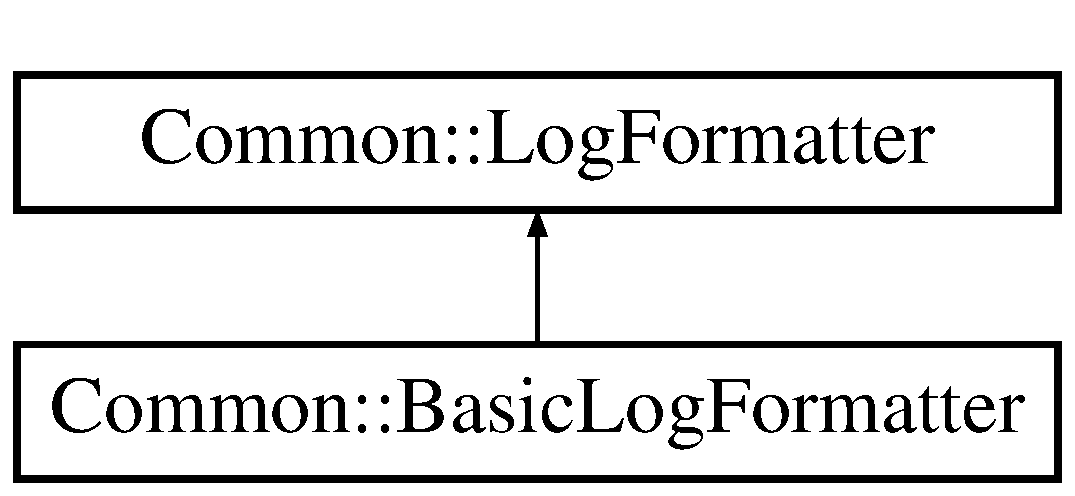
\includegraphics[height=2.000000cm]{class_common_1_1_basic_log_formatter}
\end{center}
\end{figure}
\subsection*{Public Member Functions}
\begin{DoxyCompactItemize}
\item 
\hypertarget{class_common_1_1_basic_log_formatter_a222b31419556695e1e824a3bac91de21}{\hyperlink{class_common_1_1_basic_log_formatter_a222b31419556695e1e824a3bac91de21}{Basic\-Log\-Formatter} ()}\label{class_common_1_1_basic_log_formatter_a222b31419556695e1e824a3bac91de21}

\begin{DoxyCompactList}\small\item\em Constructor. \end{DoxyCompactList}\item 
\hyperlink{class_common_1_1_basic_log_formatter_aa235218f27c5ea10eea2bbb5270e8a65}{Basic\-Log\-Formatter} (\hyperlink{class_common_1_1_config}{Config} \&cfg)
\begin{DoxyCompactList}\small\item\em Constructor. \end{DoxyCompactList}\item 
\hypertarget{class_common_1_1_basic_log_formatter_a01e4739ce34a498897f7845ce91206f5}{std\-::string \hyperlink{class_common_1_1_basic_log_formatter_a01e4739ce34a498897f7845ce91206f5}{Get\-Log\-Header} () const }\label{class_common_1_1_basic_log_formatter_a01e4739ce34a498897f7845ce91206f5}

\begin{DoxyCompactList}\small\item\em Returns a string containing the log header. \end{DoxyCompactList}\item 
\hypertarget{class_common_1_1_basic_log_formatter_ae4208ec2997454c571672de0dcdc3051}{std\-::string \hyperlink{class_common_1_1_basic_log_formatter_ae4208ec2997454c571672de0dcdc3051}{Get\-Log\-Footer} () const }\label{class_common_1_1_basic_log_formatter_ae4208ec2997454c571672de0dcdc3051}

\begin{DoxyCompactList}\small\item\em Returns a string containing the log footer. \end{DoxyCompactList}\item 
\hypertarget{class_common_1_1_basic_log_formatter_a3abc6346a953c56745df04acb7d30067}{std\-::string \hyperlink{class_common_1_1_basic_log_formatter_a3abc6346a953c56745df04acb7d30067}{Format} (\hyperlink{class_common_1_1_log_entry}{Log\-Entry} const \&entry) const }\label{class_common_1_1_basic_log_formatter_a3abc6346a953c56745df04acb7d30067}

\begin{DoxyCompactList}\small\item\em Returns a string containing the \hyperlink{class_common_1_1_log_entry}{Log\-Entry} object formatted. \end{DoxyCompactList}\item 
\hypertarget{class_common_1_1_basic_log_formatter_a172fd032eda1aeeab28e41e05e3beea4}{void \hyperlink{class_common_1_1_basic_log_formatter_a172fd032eda1aeeab28e41e05e3beea4}{Show\-Timestamp} (bool value)}\label{class_common_1_1_basic_log_formatter_a172fd032eda1aeeab28e41e05e3beea4}

\begin{DoxyCompactList}\small\item\em Enables the timestamp view. \end{DoxyCompactList}\item 
\hypertarget{class_common_1_1_basic_log_formatter_aa6d2d80418ac6335050ee02bdf13f437}{void \hyperlink{class_common_1_1_basic_log_formatter_aa6d2d80418ac6335050ee02bdf13f437}{Show\-Severity} (bool value)}\label{class_common_1_1_basic_log_formatter_aa6d2d80418ac6335050ee02bdf13f437}

\begin{DoxyCompactList}\small\item\em Enables the severity view. \end{DoxyCompactList}\item 
\hypertarget{class_common_1_1_basic_log_formatter_a209956bbe8d7fba142adecb0208c1093}{void \hyperlink{class_common_1_1_basic_log_formatter_a209956bbe8d7fba142adecb0208c1093}{Show\-Channel} (bool value)}\label{class_common_1_1_basic_log_formatter_a209956bbe8d7fba142adecb0208c1093}

\begin{DoxyCompactList}\small\item\em Enables the channel view. \end{DoxyCompactList}\end{DoxyCompactItemize}


\subsection{Detailed Description}
Formats \hyperlink{class_common_1_1_log_entry}{Log\-Entry} objects to be inserted in a log. 

\begin{DoxyVersion}{Version}
1.\-0b 
\end{DoxyVersion}
\begin{DoxySince}{Since}
1.\-0b 
\end{DoxySince}
\begin{DoxyAuthor}{Author}
Ania Sikora, 2002 
\end{DoxyAuthor}


\subsection{Constructor \& Destructor Documentation}
\hypertarget{class_common_1_1_basic_log_formatter_aa235218f27c5ea10eea2bbb5270e8a65}{\index{Common\-::\-Basic\-Log\-Formatter@{Common\-::\-Basic\-Log\-Formatter}!Basic\-Log\-Formatter@{Basic\-Log\-Formatter}}
\index{Basic\-Log\-Formatter@{Basic\-Log\-Formatter}!Common::BasicLogFormatter@{Common\-::\-Basic\-Log\-Formatter}}
\subsubsection[{Basic\-Log\-Formatter}]{\setlength{\rightskip}{0pt plus 5cm}Basic\-Log\-Formatter\-::\-Basic\-Log\-Formatter (
\begin{DoxyParamCaption}
\item[{{\bf Config} \&}]{cfg}
\end{DoxyParamCaption}
)}}\label{class_common_1_1_basic_log_formatter_aa235218f27c5ea10eea2bbb5270e8a65}


Constructor. 


\begin{DoxyParams}{Parameters}
{\em cfg} & A \hyperlink{class_common_1_1_config}{Config} object containing initial settings of the log formatter. \\
\hline
\end{DoxyParams}


The documentation for this class was generated from the following files\-:\begin{DoxyCompactItemize}
\item 
Common/Syslog.\-h\item 
Common/Syslog.\-cpp\end{DoxyCompactItemize}

\hypertarget{class_common_1_1_basic_logger}{\section{Common\-:\-:Basic\-Logger Class Reference}
\label{class_common_1_1_basic_logger}\index{Common\-::\-Basic\-Logger@{Common\-::\-Basic\-Logger}}
}


Stores information of events in a system.  




{\ttfamily \#include $<$Syslog.\-h$>$}

Inheritance diagram for Common\-:\-:Basic\-Logger\-:\begin{figure}[H]
\begin{center}
\leavevmode
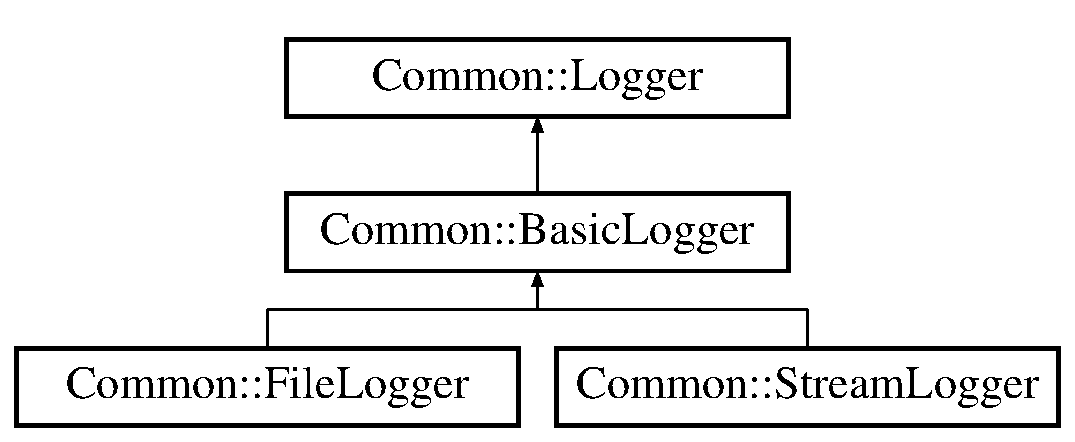
\includegraphics[height=3.000000cm]{class_common_1_1_basic_logger}
\end{center}
\end{figure}
\subsection*{Public Member Functions}
\begin{DoxyCompactItemize}
\item 
\hypertarget{class_common_1_1_basic_logger_ad36be68b705a5e866efb7e82edb40861}{\hyperlink{class_common_1_1_basic_logger_ad36be68b705a5e866efb7e82edb40861}{Basic\-Logger} ()}\label{class_common_1_1_basic_logger_ad36be68b705a5e866efb7e82edb40861}

\begin{DoxyCompactList}\small\item\em Constructor. \end{DoxyCompactList}\item 
\hypertarget{class_common_1_1_basic_logger_a70a3db86ad742d5f444722825b8fb8cc}{void \hyperlink{class_common_1_1_basic_logger_a70a3db86ad742d5f444722825b8fb8cc}{Set\-Filter} (Log\-Filter\-Ptr \&filter)}\label{class_common_1_1_basic_logger_a70a3db86ad742d5f444722825b8fb8cc}

\begin{DoxyCompactList}\small\item\em Sets the \hyperlink{class_common_1_1_log_filter}{Log\-Filter} to be used by the logger. \end{DoxyCompactList}\item 
\hypertarget{class_common_1_1_basic_logger_ab65a233cdf5b7bb8c1e4f4c031207d92}{\hyperlink{class_common_1_1_log_filter}{Log\-Filter} const $\ast$ \hyperlink{class_common_1_1_basic_logger_ab65a233cdf5b7bb8c1e4f4c031207d92}{Get\-Filter} () const }\label{class_common_1_1_basic_logger_ab65a233cdf5b7bb8c1e4f4c031207d92}

\begin{DoxyCompactList}\small\item\em Returns the \hyperlink{class_common_1_1_log_filter}{Log\-Filter} the logger uses. \end{DoxyCompactList}\item 
\hypertarget{class_common_1_1_basic_logger_ab5fd74a36a2c1ac3147c60cb1baf94f2}{void \hyperlink{class_common_1_1_basic_logger_ab5fd74a36a2c1ac3147c60cb1baf94f2}{Set\-Formatter} (Log\-Formatter\-Ptr \&formatter)}\label{class_common_1_1_basic_logger_ab5fd74a36a2c1ac3147c60cb1baf94f2}

\begin{DoxyCompactList}\small\item\em Sets the \hyperlink{class_common_1_1_log_formatter}{Log\-Formatter} to be used by the logger. \end{DoxyCompactList}\item 
\hypertarget{class_common_1_1_basic_logger_a682266d982b8b8b10958dbbfbdaa40bc}{\hyperlink{class_common_1_1_log_formatter}{Log\-Formatter} const $\ast$ \hyperlink{class_common_1_1_basic_logger_a682266d982b8b8b10958dbbfbdaa40bc}{Get\-Formatter} () const }\label{class_common_1_1_basic_logger_a682266d982b8b8b10958dbbfbdaa40bc}

\begin{DoxyCompactList}\small\item\em Returns the \hyperlink{class_common_1_1_log_formatter}{Log\-Formatter} the logger uses. \end{DoxyCompactList}\item 
bool \hyperlink{class_common_1_1_basic_logger_af9c0305a3341255bf7360be4f8f582c8}{Accept} (\hyperlink{class_common_1_1_log_entry}{Log\-Entry} const \&entry) const 
\begin{DoxyCompactList}\small\item\em Inserts an entry to the log. \end{DoxyCompactList}\end{DoxyCompactItemize}
\subsection*{Protected Attributes}
\begin{DoxyCompactItemize}
\item 
\hypertarget{class_common_1_1_basic_logger_a9d99b4bb0e48f2b4e8ebbb552f3776d3}{Log\-Filter\-Ptr {\bfseries \-\_\-filter}}\label{class_common_1_1_basic_logger_a9d99b4bb0e48f2b4e8ebbb552f3776d3}

\item 
\hypertarget{class_common_1_1_basic_logger_a0642371048e5855fa99b1392b0b52ccd}{Log\-Formatter\-Ptr {\bfseries \-\_\-formatter}}\label{class_common_1_1_basic_logger_a0642371048e5855fa99b1392b0b52ccd}

\end{DoxyCompactItemize}


\subsection{Detailed Description}
Stores information of events in a system. 

\begin{DoxyVersion}{Version}
1.\-0b 
\end{DoxyVersion}
\begin{DoxySince}{Since}
1.\-0b 
\end{DoxySince}
\begin{DoxyAuthor}{Author}
Ania Sikora, 2002 
\end{DoxyAuthor}


\subsection{Member Function Documentation}
\hypertarget{class_common_1_1_basic_logger_af9c0305a3341255bf7360be4f8f582c8}{\index{Common\-::\-Basic\-Logger@{Common\-::\-Basic\-Logger}!Accept@{Accept}}
\index{Accept@{Accept}!Common::BasicLogger@{Common\-::\-Basic\-Logger}}
\subsubsection[{Accept}]{\setlength{\rightskip}{0pt plus 5cm}bool Basic\-Logger\-::\-Accept (
\begin{DoxyParamCaption}
\item[{{\bf Log\-Entry} const \&}]{entry}
\end{DoxyParamCaption}
) const}}\label{class_common_1_1_basic_logger_af9c0305a3341255bf7360be4f8f582c8}


Inserts an entry to the log. 

\begin{DoxyReturn}{Returns}
True if the insert was successful, false otherwise. 
\end{DoxyReturn}


The documentation for this class was generated from the following files\-:\begin{DoxyCompactItemize}
\item 
Common/Syslog.\-h\item 
Common/Syslog.\-cpp\end{DoxyCompactItemize}

\hypertarget{class_batch_data}{\section{Batch\-Data Class Reference}
\label{class_batch_data}\index{Batch\-Data@{Batch\-Data}}
}


Statistics of a single batch.  




{\ttfamily \#include $<$Factoring\-Stats\-\_\-nw.\-h$>$}

\subsection*{Public Member Functions}
\begin{DoxyCompactItemize}
\item 
\hyperlink{class_batch_data_a42d0d69acb80a85ab740fd5bdc933051}{Batch\-Data} (int batch\-Idx)
\begin{DoxyCompactList}\small\item\em Constructor. \end{DoxyCompactList}\item 
\hypertarget{class_batch_data_ad55477d0f59b5076e7efcc7711c04e90}{\hyperlink{class_batch_data_ad55477d0f59b5076e7efcc7711c04e90}{$\sim$\-Batch\-Data} ()}\label{class_batch_data_ad55477d0f59b5076e7efcc7711c04e90}

\begin{DoxyCompactList}\small\item\em Destructor. \end{DoxyCompactList}\item 
void \hyperlink{class_batch_data_a47092a16aeb1356f6932c7a5ce71c773}{On\-New\-Batch} (int num\-Chunks)
\begin{DoxyCompactList}\small\item\em Sets the number of chunks to {\itshape num\-Chunks} \end{DoxyCompactList}\item 
\hyperlink{class_worker_data}{Worker\-Data} \& \hyperlink{class_batch_data_a73d104e92d0272450f0d799eba8df047}{Get\-Worker\-Data} (int worker\-Tid)
\begin{DoxyCompactList}\small\item\em Getter of the data in worker given by worker\-Tid. If it does not exist, creates a new one and returns it. \end{DoxyCompactList}\item 
\hyperlink{class_worker_data}{Worker\-Data} \& \hyperlink{class_batch_data_a02cba9872dac0dc3e0f622149e14fd8f}{New\-Worker\-Data} (int worker\-Tid)
\begin{DoxyCompactList}\small\item\em Creates a new worker data in worker\-Tid and returns it. If it already exists, returns it. \end{DoxyCompactList}\item 
bool \hyperlink{class_batch_data_a2cb14e2d5412511ee26e5d6a1006d042}{Is\-Complete} () const 
\begin{DoxyCompactList}\small\item\em Checks if the current \hyperlink{class_batch_data}{Batch\-Data} is complete. \end{DoxyCompactList}\item 
bool \hyperlink{class_batch_data_adf1ee749495ff1cd84df96123e15e70a}{Is\-Actualize} () const 
\begin{DoxyCompactList}\small\item\em Getter of the \-\_\-flag\-Actualize private var. \end{DoxyCompactList}\item 
\hypertarget{class_batch_data_a27f36cd98d28c146d5c3f097d0d81fe4}{void \hyperlink{class_batch_data_a27f36cd98d28c146d5c3f097d0d81fe4}{Set\-Actualize} ()}\label{class_batch_data_a27f36cd98d28c146d5c3f097d0d81fe4}

\begin{DoxyCompactList}\small\item\em Sets \-\_\-flag\-Actualize to 1. \end{DoxyCompactList}\item 
bool \hyperlink{class_batch_data_ab599097b9e1f7fba2ad3b829ea80f266}{Are\-Workers\-Complete} () const 
\begin{DoxyCompactList}\small\item\em Checks if all the workers {\bfseries in \hyperlink{class_batch_data}{Batch\-Data}} are complete. \end{DoxyCompactList}\item 
\hyperlink{class_worker_data}{Worker\-Data} $\ast$$\ast$ \hyperlink{class_batch_data_aae7833fddc7826d093346e80c4b3eac6}{Alloc\-Workers\-Array} ()
\begin{DoxyCompactList}\small\item\em Allocates a dynamic array of \hyperlink{class_worker_data}{Worker\-Data} and returns it. \end{DoxyCompactList}\item 
double \hyperlink{class_batch_data_a68289b65f403f6b6a965cec4a2ceaa9e}{Deviation\-Computing\-Time} ()
\begin{DoxyCompactList}\small\item\em Not implemented. \end{DoxyCompactList}\item 
double \hyperlink{class_batch_data_a09cf749b9fbad1213a44c19346b1bb14}{Mean\-Computing\-Time} ()
\begin{DoxyCompactList}\small\item\em Not implemented. \end{DoxyCompactList}\item 
int \hyperlink{class_batch_data_ab2aa288ef12cf1f45b9bde2491c64178}{Get\-Num\-Chunks} () const 
\begin{DoxyCompactList}\small\item\em Getter of \-\_\-num\-Chunks. \end{DoxyCompactList}\item 
double \hyperlink{class_batch_data_ab44cab5811e64dcde891f900964ac2c8}{Get\-Mean\-Stats} ()
\begin{DoxyCompactList}\small\item\em Calculates and returns the mean task processing time. \end{DoxyCompactList}\item 
double \hyperlink{class_batch_data_aec492a90b67eb2c2affe84f4fc865a6c}{Get\-Std\-Stats} ()
\begin{DoxyCompactList}\small\item\em Calculates and returns the standard deviation of the tasks. \end{DoxyCompactList}\item 
void \hyperlink{class_batch_data_a37ac38b8105c484df0ea907ae43e7f5b}{Size\-Task\-Received} (int size\-Tasks)
\begin{DoxyCompactList}\small\item\em Adds {\itshape size\-Tasks} to \-\_\-\-Total\-Task\-Received. \end{DoxyCompactList}\item 
int \hyperlink{class_batch_data_a4bb41517a1f0ffb1f9ade0eb1573e7ed}{Get\-Size\-Task\-Received} () const 
\begin{DoxyCompactList}\small\item\em \-\_\-\-Total\-Task\-Received getter \end{DoxyCompactList}\item 
\hyperlink{struct_model_param}{Model\-Param} \hyperlink{class_batch_data_a8c6236018210381ec747c48be7623354}{Get\-Model\-Param} ()
\begin{DoxyCompactList}\small\item\em Returns the \hyperlink{struct_model_param}{Model\-Param} object with Total\-Data\-Volume, Total\-Data\-Send\-W and Total\-Comp\-Time updated. \end{DoxyCompactList}\end{DoxyCompactItemize}


\subsection{Detailed Description}
Statistics of a single batch. 

\subsection{Constructor \& Destructor Documentation}
\hypertarget{class_batch_data_a42d0d69acb80a85ab740fd5bdc933051}{\index{Batch\-Data@{Batch\-Data}!Batch\-Data@{Batch\-Data}}
\index{Batch\-Data@{Batch\-Data}!BatchData@{Batch\-Data}}
\subsubsection[{Batch\-Data}]{\setlength{\rightskip}{0pt plus 5cm}Batch\-Data\-::\-Batch\-Data (
\begin{DoxyParamCaption}
\item[{int}]{batch\-Idx}
\end{DoxyParamCaption}
)}}\label{class_batch_data_a42d0d69acb80a85ab740fd5bdc933051}


Constructor. 


\begin{DoxyParams}{Parameters}
{\em batch\-Idx} & \\
\hline
\end{DoxyParams}


\subsection{Member Function Documentation}
\hypertarget{class_batch_data_aae7833fddc7826d093346e80c4b3eac6}{\index{Batch\-Data@{Batch\-Data}!Alloc\-Workers\-Array@{Alloc\-Workers\-Array}}
\index{Alloc\-Workers\-Array@{Alloc\-Workers\-Array}!BatchData@{Batch\-Data}}
\subsubsection[{Alloc\-Workers\-Array}]{\setlength{\rightskip}{0pt plus 5cm}{\bf Worker\-Data} $\ast$$\ast$ Batch\-Data\-::\-Alloc\-Workers\-Array (
\begin{DoxyParamCaption}
{}
\end{DoxyParamCaption}
)}}\label{class_batch_data_aae7833fddc7826d093346e80c4b3eac6}


Allocates a dynamic array of \hyperlink{class_worker_data}{Worker\-Data} and returns it. 

\begin{DoxyReturn}{Returns}
\hyperlink{class_worker_data}{Worker\-Data} array 
\end{DoxyReturn}
\hypertarget{class_batch_data_ab599097b9e1f7fba2ad3b829ea80f266}{\index{Batch\-Data@{Batch\-Data}!Are\-Workers\-Complete@{Are\-Workers\-Complete}}
\index{Are\-Workers\-Complete@{Are\-Workers\-Complete}!BatchData@{Batch\-Data}}
\subsubsection[{Are\-Workers\-Complete}]{\setlength{\rightskip}{0pt plus 5cm}bool Batch\-Data\-::\-Are\-Workers\-Complete (
\begin{DoxyParamCaption}
{}
\end{DoxyParamCaption}
) const}}\label{class_batch_data_ab599097b9e1f7fba2ad3b829ea80f266}


Checks if all the workers {\bfseries in \hyperlink{class_batch_data}{Batch\-Data}} are complete. 

\begin{DoxyReturn}{Returns}
boolean 
\end{DoxyReturn}
\hypertarget{class_batch_data_a68289b65f403f6b6a965cec4a2ceaa9e}{\index{Batch\-Data@{Batch\-Data}!Deviation\-Computing\-Time@{Deviation\-Computing\-Time}}
\index{Deviation\-Computing\-Time@{Deviation\-Computing\-Time}!BatchData@{Batch\-Data}}
\subsubsection[{Deviation\-Computing\-Time}]{\setlength{\rightskip}{0pt plus 5cm}double Batch\-Data\-::\-Deviation\-Computing\-Time (
\begin{DoxyParamCaption}
{}
\end{DoxyParamCaption}
)}}\label{class_batch_data_a68289b65f403f6b6a965cec4a2ceaa9e}


Not implemented. 

\begin{DoxyReturn}{Returns}

\end{DoxyReturn}
\hypertarget{class_batch_data_ab44cab5811e64dcde891f900964ac2c8}{\index{Batch\-Data@{Batch\-Data}!Get\-Mean\-Stats@{Get\-Mean\-Stats}}
\index{Get\-Mean\-Stats@{Get\-Mean\-Stats}!BatchData@{Batch\-Data}}
\subsubsection[{Get\-Mean\-Stats}]{\setlength{\rightskip}{0pt plus 5cm}double Batch\-Data\-::\-Get\-Mean\-Stats (
\begin{DoxyParamCaption}
{}
\end{DoxyParamCaption}
)}}\label{class_batch_data_ab44cab5811e64dcde891f900964ac2c8}


Calculates and returns the mean task processing time. 

\begin{DoxyReturn}{Returns}
mean time in {\bfseries seconds?} 
\end{DoxyReturn}
\hypertarget{class_batch_data_a8c6236018210381ec747c48be7623354}{\index{Batch\-Data@{Batch\-Data}!Get\-Model\-Param@{Get\-Model\-Param}}
\index{Get\-Model\-Param@{Get\-Model\-Param}!BatchData@{Batch\-Data}}
\subsubsection[{Get\-Model\-Param}]{\setlength{\rightskip}{0pt plus 5cm}{\bf Model\-Param} Batch\-Data\-::\-Get\-Model\-Param (
\begin{DoxyParamCaption}
{}
\end{DoxyParamCaption}
)}}\label{class_batch_data_a8c6236018210381ec747c48be7623354}


Returns the \hyperlink{struct_model_param}{Model\-Param} object with Total\-Data\-Volume, Total\-Data\-Send\-W and Total\-Comp\-Time updated. 

\begin{DoxyReturn}{Returns}
\hyperlink{struct_model_param}{Model\-Param} object 
\end{DoxyReturn}
\hypertarget{class_batch_data_ab2aa288ef12cf1f45b9bde2491c64178}{\index{Batch\-Data@{Batch\-Data}!Get\-Num\-Chunks@{Get\-Num\-Chunks}}
\index{Get\-Num\-Chunks@{Get\-Num\-Chunks}!BatchData@{Batch\-Data}}
\subsubsection[{Get\-Num\-Chunks}]{\setlength{\rightskip}{0pt plus 5cm}int Batch\-Data\-::\-Get\-Num\-Chunks (
\begin{DoxyParamCaption}
{}
\end{DoxyParamCaption}
) const\hspace{0.3cm}{\ttfamily [inline]}}}\label{class_batch_data_ab2aa288ef12cf1f45b9bde2491c64178}


Getter of \-\_\-num\-Chunks. 

\begin{DoxyReturn}{Returns}
\-\_\-num\-Chunks 
\end{DoxyReturn}
\hypertarget{class_batch_data_a4bb41517a1f0ffb1f9ade0eb1573e7ed}{\index{Batch\-Data@{Batch\-Data}!Get\-Size\-Task\-Received@{Get\-Size\-Task\-Received}}
\index{Get\-Size\-Task\-Received@{Get\-Size\-Task\-Received}!BatchData@{Batch\-Data}}
\subsubsection[{Get\-Size\-Task\-Received}]{\setlength{\rightskip}{0pt plus 5cm}int Batch\-Data\-::\-Get\-Size\-Task\-Received (
\begin{DoxyParamCaption}
{}
\end{DoxyParamCaption}
) const\hspace{0.3cm}{\ttfamily [inline]}}}\label{class_batch_data_a4bb41517a1f0ffb1f9ade0eb1573e7ed}


\-\_\-\-Total\-Task\-Received getter 

\begin{DoxyReturn}{Returns}
\-\_\-\-Total\-Task\-Received 
\end{DoxyReturn}
\hypertarget{class_batch_data_aec492a90b67eb2c2affe84f4fc865a6c}{\index{Batch\-Data@{Batch\-Data}!Get\-Std\-Stats@{Get\-Std\-Stats}}
\index{Get\-Std\-Stats@{Get\-Std\-Stats}!BatchData@{Batch\-Data}}
\subsubsection[{Get\-Std\-Stats}]{\setlength{\rightskip}{0pt plus 5cm}double Batch\-Data\-::\-Get\-Std\-Stats (
\begin{DoxyParamCaption}
{}
\end{DoxyParamCaption}
)}}\label{class_batch_data_aec492a90b67eb2c2affe84f4fc865a6c}


Calculates and returns the standard deviation of the tasks. 

\begin{DoxyReturn}{Returns}
standard deviation 
\end{DoxyReturn}
\hypertarget{class_batch_data_a73d104e92d0272450f0d799eba8df047}{\index{Batch\-Data@{Batch\-Data}!Get\-Worker\-Data@{Get\-Worker\-Data}}
\index{Get\-Worker\-Data@{Get\-Worker\-Data}!BatchData@{Batch\-Data}}
\subsubsection[{Get\-Worker\-Data}]{\setlength{\rightskip}{0pt plus 5cm}{\bf Worker\-Data} \& Batch\-Data\-::\-Get\-Worker\-Data (
\begin{DoxyParamCaption}
\item[{int}]{worker\-Tid}
\end{DoxyParamCaption}
)}}\label{class_batch_data_a73d104e92d0272450f0d799eba8df047}


Getter of the data in worker given by worker\-Tid. If it does not exist, creates a new one and returns it. 


\begin{DoxyParams}{Parameters}
{\em worker\-Tid} & Worker I\-D \\
\hline
\end{DoxyParams}
\begin{DoxyReturn}{Returns}
\hyperlink{class_worker_data}{Worker\-Data} object 
\end{DoxyReturn}
\hypertarget{class_batch_data_adf1ee749495ff1cd84df96123e15e70a}{\index{Batch\-Data@{Batch\-Data}!Is\-Actualize@{Is\-Actualize}}
\index{Is\-Actualize@{Is\-Actualize}!BatchData@{Batch\-Data}}
\subsubsection[{Is\-Actualize}]{\setlength{\rightskip}{0pt plus 5cm}bool Batch\-Data\-::\-Is\-Actualize (
\begin{DoxyParamCaption}
{}
\end{DoxyParamCaption}
) const\hspace{0.3cm}{\ttfamily [inline]}}}\label{class_batch_data_adf1ee749495ff1cd84df96123e15e70a}


Getter of the \-\_\-flag\-Actualize private var. 

\begin{DoxyReturn}{Returns}
returns \-\_\-flag\-Actualize 
\end{DoxyReturn}
\hypertarget{class_batch_data_a2cb14e2d5412511ee26e5d6a1006d042}{\index{Batch\-Data@{Batch\-Data}!Is\-Complete@{Is\-Complete}}
\index{Is\-Complete@{Is\-Complete}!BatchData@{Batch\-Data}}
\subsubsection[{Is\-Complete}]{\setlength{\rightskip}{0pt plus 5cm}bool Batch\-Data\-::\-Is\-Complete (
\begin{DoxyParamCaption}
{}
\end{DoxyParamCaption}
) const\hspace{0.3cm}{\ttfamily [inline]}}}\label{class_batch_data_a2cb14e2d5412511ee26e5d6a1006d042}


Checks if the current \hyperlink{class_batch_data}{Batch\-Data} is complete. 

\begin{DoxyReturn}{Returns}
boolean 
\end{DoxyReturn}
\hypertarget{class_batch_data_a09cf749b9fbad1213a44c19346b1bb14}{\index{Batch\-Data@{Batch\-Data}!Mean\-Computing\-Time@{Mean\-Computing\-Time}}
\index{Mean\-Computing\-Time@{Mean\-Computing\-Time}!BatchData@{Batch\-Data}}
\subsubsection[{Mean\-Computing\-Time}]{\setlength{\rightskip}{0pt plus 5cm}double Batch\-Data\-::\-Mean\-Computing\-Time (
\begin{DoxyParamCaption}
{}
\end{DoxyParamCaption}
)}}\label{class_batch_data_a09cf749b9fbad1213a44c19346b1bb14}


Not implemented. 

\begin{DoxyReturn}{Returns}

\end{DoxyReturn}
\hypertarget{class_batch_data_a02cba9872dac0dc3e0f622149e14fd8f}{\index{Batch\-Data@{Batch\-Data}!New\-Worker\-Data@{New\-Worker\-Data}}
\index{New\-Worker\-Data@{New\-Worker\-Data}!BatchData@{Batch\-Data}}
\subsubsection[{New\-Worker\-Data}]{\setlength{\rightskip}{0pt plus 5cm}{\bf Worker\-Data} \& Batch\-Data\-::\-New\-Worker\-Data (
\begin{DoxyParamCaption}
\item[{int}]{worker\-Tid}
\end{DoxyParamCaption}
)}}\label{class_batch_data_a02cba9872dac0dc3e0f622149e14fd8f}


Creates a new worker data in worker\-Tid and returns it. If it already exists, returns it. 


\begin{DoxyParams}{Parameters}
{\em worker\-Tid} & Worker I\-D \\
\hline
\end{DoxyParams}
\begin{DoxyReturn}{Returns}
\hyperlink{class_worker_data}{Worker\-Data} Object 
\end{DoxyReturn}
\hypertarget{class_batch_data_a47092a16aeb1356f6932c7a5ce71c773}{\index{Batch\-Data@{Batch\-Data}!On\-New\-Batch@{On\-New\-Batch}}
\index{On\-New\-Batch@{On\-New\-Batch}!BatchData@{Batch\-Data}}
\subsubsection[{On\-New\-Batch}]{\setlength{\rightskip}{0pt plus 5cm}void Batch\-Data\-::\-On\-New\-Batch (
\begin{DoxyParamCaption}
\item[{int}]{num\-Chunks}
\end{DoxyParamCaption}
)\hspace{0.3cm}{\ttfamily [inline]}}}\label{class_batch_data_a47092a16aeb1356f6932c7a5ce71c773}


Sets the number of chunks to {\itshape num\-Chunks} 


\begin{DoxyParams}{Parameters}
{\em num\-Chunks} & Number of chunks \\
\hline
\end{DoxyParams}
\hypertarget{class_batch_data_a37ac38b8105c484df0ea907ae43e7f5b}{\index{Batch\-Data@{Batch\-Data}!Size\-Task\-Received@{Size\-Task\-Received}}
\index{Size\-Task\-Received@{Size\-Task\-Received}!BatchData@{Batch\-Data}}
\subsubsection[{Size\-Task\-Received}]{\setlength{\rightskip}{0pt plus 5cm}void Batch\-Data\-::\-Size\-Task\-Received (
\begin{DoxyParamCaption}
\item[{int}]{size\-Tasks}
\end{DoxyParamCaption}
)\hspace{0.3cm}{\ttfamily [inline]}}}\label{class_batch_data_a37ac38b8105c484df0ea907ae43e7f5b}


Adds {\itshape size\-Tasks} to \-\_\-\-Total\-Task\-Received. 


\begin{DoxyParams}{Parameters}
{\em size\-Tasks} & \\
\hline
\end{DoxyParams}


The documentation for this class was generated from the following files\-:\begin{DoxyCompactItemize}
\item 
Analyzer/Factoring\-Stats\-\_\-nw.\-h\item 
Analyzer/Factoring\-Stats\-\_\-nw.\-cpp\end{DoxyCompactItemize}

\hypertarget{class_common_1_1_breakpoint}{\section{Common\-:\-:Breakpoint Class Reference}
\label{class_common_1_1_breakpoint}\index{Common\-::\-Breakpoint@{Common\-::\-Breakpoint}}
}


Denotes place in a function (on the entry or at the end).  




{\ttfamily \#include $<$Utils.\-h$>$}

Inheritance diagram for Common\-:\-:Breakpoint\-:\begin{figure}[H]
\begin{center}
\leavevmode
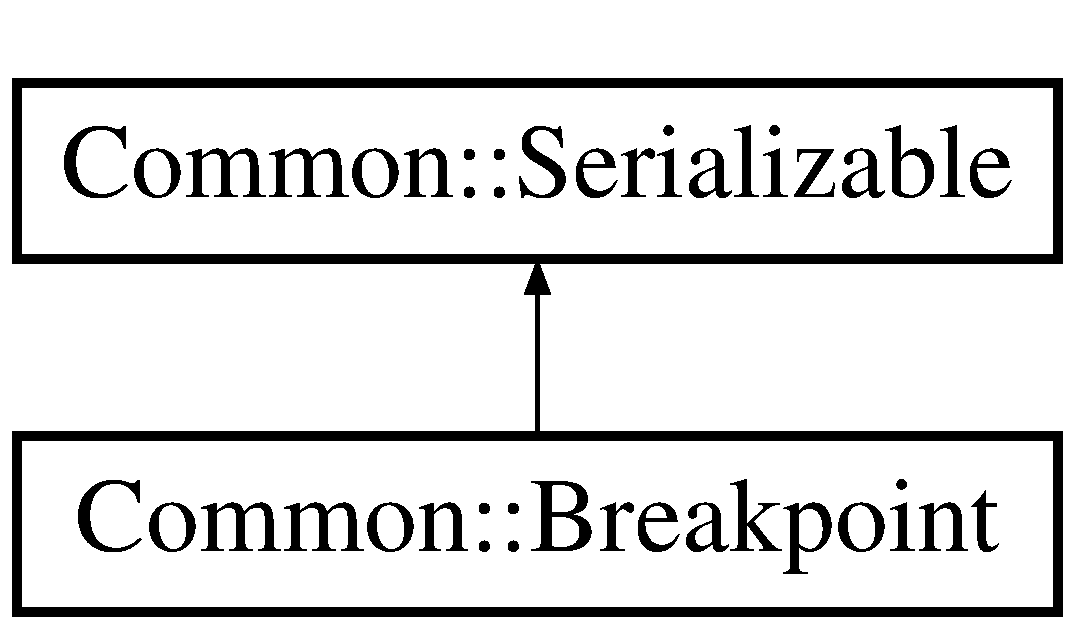
\includegraphics[height=2.000000cm]{class_common_1_1_breakpoint}
\end{center}
\end{figure}
\subsection*{Public Member Functions}
\begin{DoxyCompactItemize}
\item 
\hypertarget{class_common_1_1_breakpoint_a57e92a8c09ca8a7d86c21e900b9df14e}{\hyperlink{class_common_1_1_breakpoint_a57e92a8c09ca8a7d86c21e900b9df14e}{Breakpoint} ()}\label{class_common_1_1_breakpoint_a57e92a8c09ca8a7d86c21e900b9df14e}

\begin{DoxyCompactList}\small\item\em Constructor. \end{DoxyCompactList}\item 
\hypertarget{class_common_1_1_breakpoint_a31ab5c5a53a747d1026651dd3d38fa64}{\hyperlink{class_common_1_1_breakpoint_a31ab5c5a53a747d1026651dd3d38fa64}{Breakpoint} (\hyperlink{class_common_1_1_breakpoint}{Breakpoint} const \&b)}\label{class_common_1_1_breakpoint_a31ab5c5a53a747d1026651dd3d38fa64}

\begin{DoxyCompactList}\small\item\em Copy Constructor. \end{DoxyCompactList}\item 
\hypertarget{class_common_1_1_breakpoint_a6635c068cdda3928a48b282a8a4214e8}{void \hyperlink{class_common_1_1_breakpoint_a6635c068cdda3928a48b282a8a4214e8}{Serialize} (\hyperlink{class_common_1_1_serializer}{Serializer} \&out) const }\label{class_common_1_1_breakpoint_a6635c068cdda3928a48b282a8a4214e8}

\begin{DoxyCompactList}\small\item\em Serializes the breakpoint through the given \hyperlink{class_common_1_1_serializer}{Serializer}. \end{DoxyCompactList}\item 
\hypertarget{class_common_1_1_breakpoint_adcb23cf35fd14da188ba0369e029df95}{void \hyperlink{class_common_1_1_breakpoint_adcb23cf35fd14da188ba0369e029df95}{De\-Serialize} (\hyperlink{class_common_1_1_de_serializer}{De\-Serializer} \&in)}\label{class_common_1_1_breakpoint_adcb23cf35fd14da188ba0369e029df95}

\begin{DoxyCompactList}\small\item\em Deserializes the breakpoint from the given \hyperlink{class_common_1_1_de_serializer}{De\-Serializer}. \end{DoxyCompactList}\end{DoxyCompactItemize}
\subsection*{Public Attributes}
\begin{DoxyCompactItemize}
\item 
\hypertarget{class_common_1_1_breakpoint_a46aa1e243f9e75177c55ff2b2cdb4bb5}{std\-::string {\bfseries func\-Name}}\label{class_common_1_1_breakpoint_a46aa1e243f9e75177c55ff2b2cdb4bb5}

\item 
\hypertarget{class_common_1_1_breakpoint_ae0a7e51094dc889befb90b99e3bff8f9}{Instr\-Place {\bfseries place}}\label{class_common_1_1_breakpoint_ae0a7e51094dc889befb90b99e3bff8f9}

\end{DoxyCompactItemize}


\subsection{Detailed Description}
Denotes place in a function (on the entry or at the end). 

\begin{DoxyVersion}{Version}
1.\-0 
\end{DoxyVersion}
\begin{DoxySince}{Since}
1.\-0 
\end{DoxySince}
\begin{DoxyAuthor}{Author}
Ania Sikora, 2002 
\end{DoxyAuthor}


The documentation for this class was generated from the following file\-:\begin{DoxyCompactItemize}
\item 
Common/Utils.\-h\end{DoxyCompactItemize}

\hypertarget{class_common_1_1_byte_stream}{\section{Common\-:\-:Byte\-Stream Class Reference}
\label{class_common_1_1_byte_stream}\index{Common\-::\-Byte\-Stream@{Common\-::\-Byte\-Stream}}
}


Stores stream of bytes.  




{\ttfamily \#include $<$Byte\-Stream.\-h$>$}

Inheritance diagram for Common\-:\-:Byte\-Stream\-:\begin{figure}[H]
\begin{center}
\leavevmode
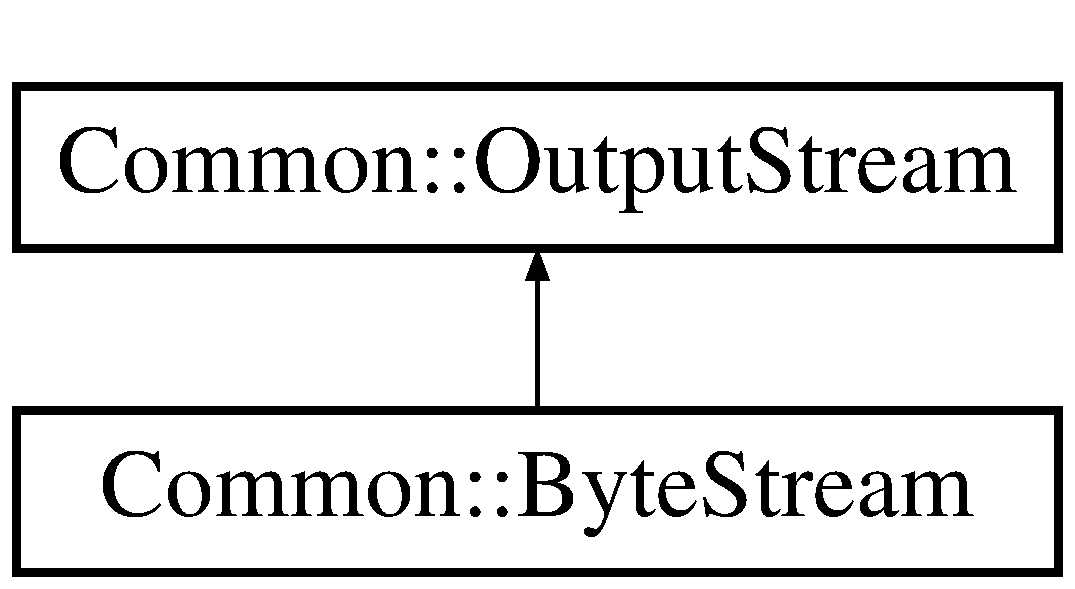
\includegraphics[height=2.000000cm]{class_common_1_1_byte_stream}
\end{center}
\end{figure}
\subsection*{Public Member Functions}
\begin{DoxyCompactItemize}
\item 
\hyperlink{class_common_1_1_byte_stream_a40d319a2f4b29672216a7cc135f2aa84}{Byte\-Stream} (char $\ast$buf, size\-\_\-t buf\-Size)
\begin{DoxyCompactList}\small\item\em Constructor. \end{DoxyCompactList}\item 
\hyperlink{class_common_1_1_byte_stream_aa98249a6d0a862fbb35ad27a1a60d01d}{Byte\-Stream} (size\-\_\-t buf\-Size)
\begin{DoxyCompactList}\small\item\em Constructor. Creates an intern buffer. \end{DoxyCompactList}\item 
void \hyperlink{class_common_1_1_byte_stream_a8ab16f23bce1e2cb0962761b9ac01be4}{Write} (char const $\ast$buf, size\-\_\-t buf\-Size)
\begin{DoxyCompactList}\small\item\em Adds the content of the buffer to the stream. \end{DoxyCompactList}\item 
char const $\ast$ \hyperlink{class_common_1_1_byte_stream_a91ca094a1637a948c279d9cab3f00887}{Get\-Data} () const 
\begin{DoxyCompactList}\small\item\em Returns pointer to the intern buffer. \end{DoxyCompactList}\item 
size\-\_\-t \hyperlink{class_common_1_1_byte_stream_a82ff2f3a9e446c716c6e0889691819d4}{Get\-Data\-Size} () const 
\begin{DoxyCompactList}\small\item\em Returns size of the stream. \end{DoxyCompactList}\item 
\hypertarget{class_common_1_1_byte_stream_a15ec1d409725f5ed875a733805bf0ba8}{void \hyperlink{class_common_1_1_byte_stream_a15ec1d409725f5ed875a733805bf0ba8}{Reset} ()}\label{class_common_1_1_byte_stream_a15ec1d409725f5ed875a733805bf0ba8}

\begin{DoxyCompactList}\small\item\em Clears the stream. \end{DoxyCompactList}\end{DoxyCompactItemize}


\subsection{Detailed Description}
Stores stream of bytes. 

\begin{DoxyVersion}{Version}
1.\-0b 
\end{DoxyVersion}
\begin{DoxySince}{Since}
1.\-0b 
\end{DoxySince}
\begin{DoxyAuthor}{Author}
Ania Sikora, 2002 
\end{DoxyAuthor}


\subsection{Constructor \& Destructor Documentation}
\hypertarget{class_common_1_1_byte_stream_a40d319a2f4b29672216a7cc135f2aa84}{\index{Common\-::\-Byte\-Stream@{Common\-::\-Byte\-Stream}!Byte\-Stream@{Byte\-Stream}}
\index{Byte\-Stream@{Byte\-Stream}!Common::ByteStream@{Common\-::\-Byte\-Stream}}
\subsubsection[{Byte\-Stream}]{\setlength{\rightskip}{0pt plus 5cm}Common\-::\-Byte\-Stream\-::\-Byte\-Stream (
\begin{DoxyParamCaption}
\item[{char $\ast$}]{buf, }
\item[{size\-\_\-t}]{buf\-Size}
\end{DoxyParamCaption}
)\hspace{0.3cm}{\ttfamily [inline]}}}\label{class_common_1_1_byte_stream_a40d319a2f4b29672216a7cc135f2aa84}


Constructor. 


\begin{DoxyParams}{Parameters}
{\em buf} & Intern buffer to be used. \\
\hline
{\em buf\-Size} & Size of the intern buffer. \\
\hline
\end{DoxyParams}
\hypertarget{class_common_1_1_byte_stream_aa98249a6d0a862fbb35ad27a1a60d01d}{\index{Common\-::\-Byte\-Stream@{Common\-::\-Byte\-Stream}!Byte\-Stream@{Byte\-Stream}}
\index{Byte\-Stream@{Byte\-Stream}!Common::ByteStream@{Common\-::\-Byte\-Stream}}
\subsubsection[{Byte\-Stream}]{\setlength{\rightskip}{0pt plus 5cm}Common\-::\-Byte\-Stream\-::\-Byte\-Stream (
\begin{DoxyParamCaption}
\item[{size\-\_\-t}]{buf\-Size}
\end{DoxyParamCaption}
)\hspace{0.3cm}{\ttfamily [inline]}}}\label{class_common_1_1_byte_stream_aa98249a6d0a862fbb35ad27a1a60d01d}


Constructor. Creates an intern buffer. 


\begin{DoxyParams}{Parameters}
{\em buf\-Size} & Size of the intern buffer. \\
\hline
\end{DoxyParams}


\subsection{Member Function Documentation}
\hypertarget{class_common_1_1_byte_stream_a91ca094a1637a948c279d9cab3f00887}{\index{Common\-::\-Byte\-Stream@{Common\-::\-Byte\-Stream}!Get\-Data@{Get\-Data}}
\index{Get\-Data@{Get\-Data}!Common::ByteStream@{Common\-::\-Byte\-Stream}}
\subsubsection[{Get\-Data}]{\setlength{\rightskip}{0pt plus 5cm}char const$\ast$ Common\-::\-Byte\-Stream\-::\-Get\-Data (
\begin{DoxyParamCaption}
{}
\end{DoxyParamCaption}
) const\hspace{0.3cm}{\ttfamily [inline]}}}\label{class_common_1_1_byte_stream_a91ca094a1637a948c279d9cab3f00887}


Returns pointer to the intern buffer. 

When used the returned pointer should always use the \hyperlink{class_common_1_1_byte_stream_a82ff2f3a9e446c716c6e0889691819d4}{Get\-Data\-Size()} method to iterate over the buffer.

\begin{DoxyReturn}{Returns}
Read-\/only pointer to the intern buffer. 
\end{DoxyReturn}
\hypertarget{class_common_1_1_byte_stream_a82ff2f3a9e446c716c6e0889691819d4}{\index{Common\-::\-Byte\-Stream@{Common\-::\-Byte\-Stream}!Get\-Data\-Size@{Get\-Data\-Size}}
\index{Get\-Data\-Size@{Get\-Data\-Size}!Common::ByteStream@{Common\-::\-Byte\-Stream}}
\subsubsection[{Get\-Data\-Size}]{\setlength{\rightskip}{0pt plus 5cm}size\-\_\-t Common\-::\-Byte\-Stream\-::\-Get\-Data\-Size (
\begin{DoxyParamCaption}
{}
\end{DoxyParamCaption}
) const\hspace{0.3cm}{\ttfamily [inline]}}}\label{class_common_1_1_byte_stream_a82ff2f3a9e446c716c6e0889691819d4}


Returns size of the stream. 

\begin{DoxyReturn}{Returns}
Buffer size. 
\end{DoxyReturn}
\hypertarget{class_common_1_1_byte_stream_a8ab16f23bce1e2cb0962761b9ac01be4}{\index{Common\-::\-Byte\-Stream@{Common\-::\-Byte\-Stream}!Write@{Write}}
\index{Write@{Write}!Common::ByteStream@{Common\-::\-Byte\-Stream}}
\subsubsection[{Write}]{\setlength{\rightskip}{0pt plus 5cm}void Byte\-Stream\-::\-Write (
\begin{DoxyParamCaption}
\item[{char const $\ast$}]{buf, }
\item[{size\-\_\-t}]{buf\-Size}
\end{DoxyParamCaption}
)\hspace{0.3cm}{\ttfamily [virtual]}}}\label{class_common_1_1_byte_stream_a8ab16f23bce1e2cb0962761b9ac01be4}


Adds the content of the buffer to the stream. 


\begin{DoxyParams}{Parameters}
{\em buf} & Buffer to read. \\
\hline
{\em buf\-Size} & Size of the given buffer. \\
\hline
\end{DoxyParams}


Implements \hyperlink{class_common_1_1_output_stream}{Common\-::\-Output\-Stream}.



The documentation for this class was generated from the following files\-:\begin{DoxyCompactItemize}
\item 
Common/Byte\-Stream.\-h\item 
Common/Byte\-Stream.\-cpp\end{DoxyCompactItemize}

\hypertarget{class_command_line}{\section{Command\-Line Class Reference}
\label{class_command_line}\index{Command\-Line@{Command\-Line}}
}


Encapsulates methods to interact with the user of analyzer. Basically reads the arguments of the analyzer and parses them to get the configuration file and the objective application with its parameters. Once read, encapsulates the information and provides accessors to it. There are two formats \hyperlink{class_analyzer}{Analyzer} can be called\-:  




{\ttfamily \#include $<$cmdline.\-h$>$}

\subsection*{Public Member Functions}
\begin{DoxyCompactItemize}
\item 
\hypertarget{class_command_line_a60e98cded6040cc7ba4ad64361809ddd}{\hyperlink{class_command_line_a60e98cded6040cc7ba4ad64361809ddd}{Command\-Line} (int argc, char $\ast$$\ast$argv)}\label{class_command_line_a60e98cded6040cc7ba4ad64361809ddd}

\begin{DoxyCompactList}\small\item\em Constructor. \end{DoxyCompactList}\item 
bool \hyperlink{class_command_line_a6651a1fa1136fef801c262e9801ea419}{Is\-Ok} () const 
\begin{DoxyCompactList}\small\item\em Returns the value of \-\_\-is\-Ok. \end{DoxyCompactList}\item 
int \hyperlink{class_command_line_a5f3c2a10763e81dc91dfa2b8affbb1c7}{Get\-Argc} () const 
\begin{DoxyCompactList}\small\item\em Getter for the \-\_\-argc variable. \end{DoxyCompactList}\item 
char $\ast$$\ast$ \hyperlink{class_command_line_a5e82914e4fc19968843cbaec712f627c}{Get\-Argv} () const 
\begin{DoxyCompactList}\small\item\em Getter for the \-\_\-argv variable. \end{DoxyCompactList}\item 
int \hyperlink{class_command_line_ac420a15eac8608dd0eacf36e8e09e913}{Get\-App\-Argc} () const 
\begin{DoxyCompactList}\small\item\em Getter for the \-\_\-app\-Argc variable. \end{DoxyCompactList}\item 
char $\ast$ \hyperlink{class_command_line_ade0b4faec1c6c947cbe3cd1d8da563ef}{Get\-App\-Path} () const 
\begin{DoxyCompactList}\small\item\em Getter for the \-\_\-app\-Path variable. \end{DoxyCompactList}\item 
char $\ast$$\ast$ \hyperlink{class_command_line_ad0632810d7d2b73f7f362f419d2c58fa}{Get\-App\-Argv} () const 
\begin{DoxyCompactList}\small\item\em Getter for the \-\_\-app\-Argv variable. \end{DoxyCompactList}\item 
bool \hyperlink{class_command_line_a1ef3920d53a63e97dbc3c823b1bf5060}{Has\-Config} () const 
\begin{DoxyCompactList}\small\item\em Checks if there's a path for the configuration file, if not returns 0. \end{DoxyCompactList}\item 
char $\ast$ \hyperlink{class_command_line_af0398729ceaef3b9660915eb7ae730b8}{Get\-Config\-File\-Name} () const 
\begin{DoxyCompactList}\small\item\em Getter for the \-\_\-config\-File variable. \end{DoxyCompactList}\item 
\hypertarget{class_command_line_a6709a77ba7fc2d93e79526583481616b}{void \hyperlink{class_command_line_a6709a77ba7fc2d93e79526583481616b}{Display\-Help} () const }\label{class_command_line_a6709a77ba7fc2d93e79526583481616b}

\begin{DoxyCompactList}\small\item\em Prints help message on the terminal. Tells the user how to introduce the necessary arguments. \end{DoxyCompactList}\item 
\hyperlink{class_command_line_a60e98cded6040cc7ba4ad64361809ddd}{Command\-Line} (int argc, char $\ast$$\ast$argv)
\begin{DoxyCompactList}\small\item\em Constructor, parses the arguments provided to analyzer. \end{DoxyCompactList}\item 
bool \hyperlink{class_command_line_a6651a1fa1136fef801c262e9801ea419}{Is\-Ok} () const 
\begin{DoxyCompactList}\small\item\em Status of the arguments getter. \end{DoxyCompactList}\item 
int \hyperlink{class_command_line_a5f3c2a10763e81dc91dfa2b8affbb1c7}{Get\-Argc} () const 
\begin{DoxyCompactList}\small\item\em Number of arguments getter. \end{DoxyCompactList}\item 
char $\ast$$\ast$ \hyperlink{class_command_line_a5e82914e4fc19968843cbaec712f627c}{Get\-Argv} () const 
\begin{DoxyCompactList}\small\item\em Arguments getter. \end{DoxyCompactList}\item 
bool \hyperlink{class_command_line_a1ef3920d53a63e97dbc3c823b1bf5060}{Has\-Config} () const 
\begin{DoxyCompactList}\small\item\em Determines if the user has chosen his own configuration file. \end{DoxyCompactList}\item 
char $\ast$ \hyperlink{class_command_line_a3f0aaa56fbbb79af92d4d91d853ea23c}{Get\-Config\-File} () const 
\begin{DoxyCompactList}\small\item\em Configuration file getter. \end{DoxyCompactList}\item 
char const $\ast$ \hyperlink{class_command_line_a75d2c3e1757396de574c1375526a3f3f}{Get\-App\-Path} () const 
\begin{DoxyCompactList}\small\item\em Application path getter. \end{DoxyCompactList}\item 
int \hyperlink{class_command_line_ac420a15eac8608dd0eacf36e8e09e913}{Get\-App\-Argc} () const 
\begin{DoxyCompactList}\small\item\em Application number of arguments getter. \end{DoxyCompactList}\item 
char const $\ast$$\ast$ \hyperlink{class_command_line_a96c4896292425152d4200ff2a6821c22}{Get\-App\-Argv} () const 
\begin{DoxyCompactList}\small\item\em Application arguments getter. \end{DoxyCompactList}\item 
\hypertarget{class_command_line_a6709a77ba7fc2d93e79526583481616b}{void \hyperlink{class_command_line_a6709a77ba7fc2d93e79526583481616b}{Display\-Help} () const }\label{class_command_line_a6709a77ba7fc2d93e79526583481616b}

\begin{DoxyCompactList}\small\item\em Explains the user which arguments can be provided to analyzer. \end{DoxyCompactList}\end{DoxyCompactItemize}


\subsection{Detailed Description}
Encapsulates methods to interact with the user of analyzer. Basically reads the arguments of the analyzer and parses them to get the configuration file and the objective application with its parameters. Once read, encapsulates the information and provides accessors to it. There are two formats \hyperlink{class_analyzer}{Analyzer} can be called\-: 

Checks for the necessary data in the arguments passed to main and parses them.


\begin{DoxyItemize}
\item \hyperlink{class_analyzer}{Analyzer} $<$\-App\-Path$>$ \mbox{[}$<$\-App\-Args$>$\mbox{]}  
\item \hyperlink{class_analyzer}{Analyzer} -\/config file.\-ini $<$\-App$>$ \mbox{[}$<$\-App\-Args$>$\mbox{]}  
\end{DoxyItemize}

Notes

\begin{DoxyVersion}{Version}
1.\-0 
\end{DoxyVersion}
\begin{DoxySince}{Since}
1.\-0 
\end{DoxySince}
\begin{DoxyAuthor}{Author}
Ania Sikora, 2002 
\end{DoxyAuthor}


\subsection{Constructor \& Destructor Documentation}
\hypertarget{class_command_line_a60e98cded6040cc7ba4ad64361809ddd}{\index{Command\-Line@{Command\-Line}!Command\-Line@{Command\-Line}}
\index{Command\-Line@{Command\-Line}!CommandLine@{Command\-Line}}
\subsubsection[{Command\-Line}]{\setlength{\rightskip}{0pt plus 5cm}Command\-Line\-::\-Command\-Line (
\begin{DoxyParamCaption}
\item[{int}]{argc, }
\item[{char $\ast$$\ast$}]{argv}
\end{DoxyParamCaption}
)\hspace{0.3cm}{\ttfamily [inline]}}}\label{class_command_line_a60e98cded6040cc7ba4ad64361809ddd}


Constructor, parses the arguments provided to analyzer. 


\begin{DoxyParams}{Parameters}
{\em argc} & number of arguments for analyzer \\
\hline
{\em argv} & arguments for analyzer \\
\hline
\end{DoxyParams}


\subsection{Member Function Documentation}
\hypertarget{class_command_line_ac420a15eac8608dd0eacf36e8e09e913}{\index{Command\-Line@{Command\-Line}!Get\-App\-Argc@{Get\-App\-Argc}}
\index{Get\-App\-Argc@{Get\-App\-Argc}!CommandLine@{Command\-Line}}
\subsubsection[{Get\-App\-Argc}]{\setlength{\rightskip}{0pt plus 5cm}int Command\-Line\-::\-Get\-App\-Argc (
\begin{DoxyParamCaption}
{}
\end{DoxyParamCaption}
) const\hspace{0.3cm}{\ttfamily [inline]}}}\label{class_command_line_ac420a15eac8608dd0eacf36e8e09e913}


Getter for the \-\_\-app\-Argc variable. 

\begin{DoxyReturn}{Returns}
Size of the arguments vector for the app. 
\end{DoxyReturn}
\hypertarget{class_command_line_ac420a15eac8608dd0eacf36e8e09e913}{\index{Command\-Line@{Command\-Line}!Get\-App\-Argc@{Get\-App\-Argc}}
\index{Get\-App\-Argc@{Get\-App\-Argc}!CommandLine@{Command\-Line}}
\subsubsection[{Get\-App\-Argc}]{\setlength{\rightskip}{0pt plus 5cm}int Command\-Line\-::\-Get\-App\-Argc (
\begin{DoxyParamCaption}
{}
\end{DoxyParamCaption}
) const\hspace{0.3cm}{\ttfamily [inline]}}}\label{class_command_line_ac420a15eac8608dd0eacf36e8e09e913}


Application number of arguments getter. 

\begin{DoxyReturn}{Returns}
The number of arguments of the target application. 
\end{DoxyReturn}
\hypertarget{class_command_line_ad0632810d7d2b73f7f362f419d2c58fa}{\index{Command\-Line@{Command\-Line}!Get\-App\-Argv@{Get\-App\-Argv}}
\index{Get\-App\-Argv@{Get\-App\-Argv}!CommandLine@{Command\-Line}}
\subsubsection[{Get\-App\-Argv}]{\setlength{\rightskip}{0pt plus 5cm}char$\ast$$\ast$ Command\-Line\-::\-Get\-App\-Argv (
\begin{DoxyParamCaption}
{}
\end{DoxyParamCaption}
) const\hspace{0.3cm}{\ttfamily [inline]}}}\label{class_command_line_ad0632810d7d2b73f7f362f419d2c58fa}


Getter for the \-\_\-app\-Argv variable. 

\begin{DoxyReturn}{Returns}
Vector that contains the app's arguments. 
\end{DoxyReturn}
\hypertarget{class_command_line_a96c4896292425152d4200ff2a6821c22}{\index{Command\-Line@{Command\-Line}!Get\-App\-Argv@{Get\-App\-Argv}}
\index{Get\-App\-Argv@{Get\-App\-Argv}!CommandLine@{Command\-Line}}
\subsubsection[{Get\-App\-Argv}]{\setlength{\rightskip}{0pt plus 5cm}char const$\ast$$\ast$ Command\-Line\-::\-Get\-App\-Argv (
\begin{DoxyParamCaption}
{}
\end{DoxyParamCaption}
) const\hspace{0.3cm}{\ttfamily [inline]}}}\label{class_command_line_a96c4896292425152d4200ff2a6821c22}


Application arguments getter. 

\begin{DoxyReturn}{Returns}
The arguments of the target application. 
\end{DoxyReturn}
\hypertarget{class_command_line_ade0b4faec1c6c947cbe3cd1d8da563ef}{\index{Command\-Line@{Command\-Line}!Get\-App\-Path@{Get\-App\-Path}}
\index{Get\-App\-Path@{Get\-App\-Path}!CommandLine@{Command\-Line}}
\subsubsection[{Get\-App\-Path}]{\setlength{\rightskip}{0pt plus 5cm}char$\ast$ Command\-Line\-::\-Get\-App\-Path (
\begin{DoxyParamCaption}
{}
\end{DoxyParamCaption}
) const\hspace{0.3cm}{\ttfamily [inline]}}}\label{class_command_line_ade0b4faec1c6c947cbe3cd1d8da563ef}


Getter for the \-\_\-app\-Path variable. 

\begin{DoxyReturn}{Returns}
Path to the executable of the app. 
\end{DoxyReturn}
\hypertarget{class_command_line_a75d2c3e1757396de574c1375526a3f3f}{\index{Command\-Line@{Command\-Line}!Get\-App\-Path@{Get\-App\-Path}}
\index{Get\-App\-Path@{Get\-App\-Path}!CommandLine@{Command\-Line}}
\subsubsection[{Get\-App\-Path}]{\setlength{\rightskip}{0pt plus 5cm}char const$\ast$ Command\-Line\-::\-Get\-App\-Path (
\begin{DoxyParamCaption}
{}
\end{DoxyParamCaption}
) const\hspace{0.3cm}{\ttfamily [inline]}}}\label{class_command_line_a75d2c3e1757396de574c1375526a3f3f}


Application path getter. 

\begin{DoxyReturn}{Returns}
The path of the target application. 
\end{DoxyReturn}
\hypertarget{class_command_line_a5f3c2a10763e81dc91dfa2b8affbb1c7}{\index{Command\-Line@{Command\-Line}!Get\-Argc@{Get\-Argc}}
\index{Get\-Argc@{Get\-Argc}!CommandLine@{Command\-Line}}
\subsubsection[{Get\-Argc}]{\setlength{\rightskip}{0pt plus 5cm}int Command\-Line\-::\-Get\-Argc (
\begin{DoxyParamCaption}
{}
\end{DoxyParamCaption}
) const\hspace{0.3cm}{\ttfamily [inline]}}}\label{class_command_line_a5f3c2a10763e81dc91dfa2b8affbb1c7}


Getter for the \-\_\-argc variable. 

\begin{DoxyReturn}{Returns}
Size of the vector of arguments. 
\end{DoxyReturn}
\hypertarget{class_command_line_a5f3c2a10763e81dc91dfa2b8affbb1c7}{\index{Command\-Line@{Command\-Line}!Get\-Argc@{Get\-Argc}}
\index{Get\-Argc@{Get\-Argc}!CommandLine@{Command\-Line}}
\subsubsection[{Get\-Argc}]{\setlength{\rightskip}{0pt plus 5cm}int Command\-Line\-::\-Get\-Argc (
\begin{DoxyParamCaption}
{}
\end{DoxyParamCaption}
) const\hspace{0.3cm}{\ttfamily [inline]}}}\label{class_command_line_a5f3c2a10763e81dc91dfa2b8affbb1c7}


Number of arguments getter. 

\begin{DoxyReturn}{Returns}
The number of arguments provided to analyzer. 
\end{DoxyReturn}
\hypertarget{class_command_line_a5e82914e4fc19968843cbaec712f627c}{\index{Command\-Line@{Command\-Line}!Get\-Argv@{Get\-Argv}}
\index{Get\-Argv@{Get\-Argv}!CommandLine@{Command\-Line}}
\subsubsection[{Get\-Argv}]{\setlength{\rightskip}{0pt plus 5cm}char$\ast$$\ast$ Command\-Line\-::\-Get\-Argv (
\begin{DoxyParamCaption}
{}
\end{DoxyParamCaption}
) const\hspace{0.3cm}{\ttfamily [inline]}}}\label{class_command_line_a5e82914e4fc19968843cbaec712f627c}


Getter for the \-\_\-argv variable. 

\begin{DoxyReturn}{Returns}
Vector of arguments. 
\end{DoxyReturn}
\hypertarget{class_command_line_a5e82914e4fc19968843cbaec712f627c}{\index{Command\-Line@{Command\-Line}!Get\-Argv@{Get\-Argv}}
\index{Get\-Argv@{Get\-Argv}!CommandLine@{Command\-Line}}
\subsubsection[{Get\-Argv}]{\setlength{\rightskip}{0pt plus 5cm}char$\ast$$\ast$ Command\-Line\-::\-Get\-Argv (
\begin{DoxyParamCaption}
{}
\end{DoxyParamCaption}
) const\hspace{0.3cm}{\ttfamily [inline]}}}\label{class_command_line_a5e82914e4fc19968843cbaec712f627c}


Arguments getter. 

\begin{DoxyReturn}{Returns}
The arguments provided to analyzer. 
\end{DoxyReturn}
\hypertarget{class_command_line_a3f0aaa56fbbb79af92d4d91d853ea23c}{\index{Command\-Line@{Command\-Line}!Get\-Config\-File@{Get\-Config\-File}}
\index{Get\-Config\-File@{Get\-Config\-File}!CommandLine@{Command\-Line}}
\subsubsection[{Get\-Config\-File}]{\setlength{\rightskip}{0pt plus 5cm}char$\ast$ Command\-Line\-::\-Get\-Config\-File (
\begin{DoxyParamCaption}
{}
\end{DoxyParamCaption}
) const\hspace{0.3cm}{\ttfamily [inline]}}}\label{class_command_line_a3f0aaa56fbbb79af92d4d91d853ea23c}


Configuration file getter. 

\begin{DoxyReturn}{Returns}
The configuration file of \hyperlink{class_analyzer}{Analyzer}. 
\end{DoxyReturn}
\hypertarget{class_command_line_af0398729ceaef3b9660915eb7ae730b8}{\index{Command\-Line@{Command\-Line}!Get\-Config\-File\-Name@{Get\-Config\-File\-Name}}
\index{Get\-Config\-File\-Name@{Get\-Config\-File\-Name}!CommandLine@{Command\-Line}}
\subsubsection[{Get\-Config\-File\-Name}]{\setlength{\rightskip}{0pt plus 5cm}char$\ast$ Command\-Line\-::\-Get\-Config\-File\-Name (
\begin{DoxyParamCaption}
{}
\end{DoxyParamCaption}
) const\hspace{0.3cm}{\ttfamily [inline]}}}\label{class_command_line_af0398729ceaef3b9660915eb7ae730b8}


Getter for the \-\_\-config\-File variable. 

\begin{DoxyReturn}{Returns}
Path for the configuration file. 
\end{DoxyReturn}
\hypertarget{class_command_line_a1ef3920d53a63e97dbc3c823b1bf5060}{\index{Command\-Line@{Command\-Line}!Has\-Config@{Has\-Config}}
\index{Has\-Config@{Has\-Config}!CommandLine@{Command\-Line}}
\subsubsection[{Has\-Config}]{\setlength{\rightskip}{0pt plus 5cm}bool Command\-Line\-::\-Has\-Config (
\begin{DoxyParamCaption}
{}
\end{DoxyParamCaption}
) const\hspace{0.3cm}{\ttfamily [inline]}}}\label{class_command_line_a1ef3920d53a63e97dbc3c823b1bf5060}


Determines if the user has chosen his own configuration file. 

\begin{DoxyReturn}{Returns}
If the user provided a specific configuration file. 
\end{DoxyReturn}
\hypertarget{class_command_line_a1ef3920d53a63e97dbc3c823b1bf5060}{\index{Command\-Line@{Command\-Line}!Has\-Config@{Has\-Config}}
\index{Has\-Config@{Has\-Config}!CommandLine@{Command\-Line}}
\subsubsection[{Has\-Config}]{\setlength{\rightskip}{0pt plus 5cm}bool Command\-Line\-::\-Has\-Config (
\begin{DoxyParamCaption}
{}
\end{DoxyParamCaption}
) const\hspace{0.3cm}{\ttfamily [inline]}}}\label{class_command_line_a1ef3920d53a63e97dbc3c823b1bf5060}


Checks if there's a path for the configuration file, if not returns 0. 

\begin{DoxyReturn}{Returns}
Path for the configuration file. 
\end{DoxyReturn}
\hypertarget{class_command_line_a6651a1fa1136fef801c262e9801ea419}{\index{Command\-Line@{Command\-Line}!Is\-Ok@{Is\-Ok}}
\index{Is\-Ok@{Is\-Ok}!CommandLine@{Command\-Line}}
\subsubsection[{Is\-Ok}]{\setlength{\rightskip}{0pt plus 5cm}bool Command\-Line\-::\-Is\-Ok (
\begin{DoxyParamCaption}
{}
\end{DoxyParamCaption}
) const\hspace{0.3cm}{\ttfamily [inline]}}}\label{class_command_line_a6651a1fa1136fef801c262e9801ea419}


Returns the value of \-\_\-is\-Ok. 

\begin{DoxyReturn}{Returns}
Boolean variable that is true if the configuration has been parsed correctly. 
\end{DoxyReturn}
\hypertarget{class_command_line_a6651a1fa1136fef801c262e9801ea419}{\index{Command\-Line@{Command\-Line}!Is\-Ok@{Is\-Ok}}
\index{Is\-Ok@{Is\-Ok}!CommandLine@{Command\-Line}}
\subsubsection[{Is\-Ok}]{\setlength{\rightskip}{0pt plus 5cm}bool Command\-Line\-::\-Is\-Ok (
\begin{DoxyParamCaption}
{}
\end{DoxyParamCaption}
) const\hspace{0.3cm}{\ttfamily [inline]}}}\label{class_command_line_a6651a1fa1136fef801c262e9801ea419}


Status of the arguments getter. 

\begin{DoxyReturn}{Returns}
if the arguments provided to analyzer are correct or not. 
\end{DoxyReturn}


The documentation for this class was generated from the following files\-:\begin{DoxyCompactItemize}
\item 
A\-C/cmdline.\-h\item 
Analyzer/cmdline.\-h\end{DoxyCompactItemize}

\hypertarget{class_common_1_1_config}{\section{Common\-:\-:Config Class Reference}
\label{class_common_1_1_config}\index{Common\-::\-Config@{Common\-::\-Config}}
}


Manages a configuration of the system.  




{\ttfamily \#include $<$Config.\-h$>$}

\subsection*{Classes}
\begin{DoxyCompactItemize}
\item 
class \hyperlink{class_common_1_1_config_1_1_key_iterator}{Key\-Iterator}
\begin{DoxyCompactList}\small\item\em Iterates over the keys of a \hyperlink{class_common_1_1_config}{Config} object. \end{DoxyCompactList}\end{DoxyCompactItemize}
\subsection*{Public Member Functions}
\begin{DoxyCompactItemize}
\item 
\hypertarget{class_common_1_1_config_ae5f62f67f9815ba0cb963ae78565e00d}{\hyperlink{class_common_1_1_config_ae5f62f67f9815ba0cb963ae78565e00d}{Config} ()}\label{class_common_1_1_config_ae5f62f67f9815ba0cb963ae78565e00d}

\begin{DoxyCompactList}\small\item\em Constructor. \end{DoxyCompactList}\item 
std\-::string const \& \hyperlink{class_common_1_1_config_ae4f60b0f7e86b4cf1887ec47afcdc485}{Get\-String\-Value} (std\-::string const \&section, std\-::string const \&key) const 
\begin{DoxyCompactList}\small\item\em Returns string value of the entry specified by the parameters. \end{DoxyCompactList}\item 
int \hyperlink{class_common_1_1_config_ac34ebeb553d7a1ab361346e7bb037140}{Get\-Int\-Value} (std\-::string const \&section, std\-::string const \&key) const 
\begin{DoxyCompactList}\small\item\em Returns integer value of the entry specified by the parameters. \end{DoxyCompactList}\item 
int \hyperlink{class_common_1_1_config_ae22508ea700d687afd24b2de16831afb}{Get\-Int\-Value} (std\-::string const \&section, std\-::string const \&key, int default\-Value) const 
\begin{DoxyCompactList}\small\item\em Returns integer value of the entry specified by the parameters. \end{DoxyCompactList}\item 
bool \hyperlink{class_common_1_1_config_ac5c1ff98fb84f80f3cca85fd17e494f3}{Get\-Bool\-Value} (std\-::string const \&section, std\-::string const \&key) const 
\begin{DoxyCompactList}\small\item\em Returns boolean value of the entry specified by the parameters. \end{DoxyCompactList}\item 
bool \hyperlink{class_common_1_1_config_aa802d8ef647dedec6261c330675b494b}{Get\-Bool\-Value} (std\-::string const \&section, std\-::string const \&key, bool default\-Value) const 
\begin{DoxyCompactList}\small\item\em Returns boolean value of the entry specified by the parameters. \end{DoxyCompactList}\item 
bool \hyperlink{class_common_1_1_config_a2db2d7a710a2da3c11f8f5e20267a9f5}{Contains} (std\-::string const \&section, std\-::string const \&key) const 
\begin{DoxyCompactList}\small\item\em Finds an entry on the configuration. \end{DoxyCompactList}\item 
\hyperlink{class_common_1_1_config_1_1_key_iterator}{Key\-Iterator} \hyperlink{class_common_1_1_config_a8c6a1b318de9e28f310763d2313bd69f}{Get\-Keys} (std\-::string const \&section) const 
\begin{DoxyCompactList}\small\item\em Returns an iterator of the keys inside the requested section. \end{DoxyCompactList}\item 
void \hyperlink{class_common_1_1_config_a503736d04428c150b1b1610612615d48}{Add\-Entry} (std\-::string const \&section, std\-::string const \&key, std\-::string const \&value)
\begin{DoxyCompactList}\small\item\em Adds a new entry to the configuration. \end{DoxyCompactList}\end{DoxyCompactItemize}
\subsection*{Friends}
\begin{DoxyCompactItemize}
\item 
\hypertarget{class_common_1_1_config_a4e34a259365f6965a16ab8b276d358d0}{class {\bfseries Key\-Iterator}}\label{class_common_1_1_config_a4e34a259365f6965a16ab8b276d358d0}

\item 
\hypertarget{class_common_1_1_config_ada75ae56b35b5bf88aca48da1012be67}{class {\bfseries Config\-Reader}}\label{class_common_1_1_config_ada75ae56b35b5bf88aca48da1012be67}

\end{DoxyCompactItemize}


\subsection{Detailed Description}
Manages a configuration of the system. 

The configuration is based on section and keys, and the format is the following\-: 
\begin{DoxyCode}
[section]
key = value
key = value
...

[newsection]
key = value
...
\end{DoxyCode}


\begin{DoxyVersion}{Version}
1.\-0b 
\end{DoxyVersion}
\begin{DoxySince}{Since}
1.\-0b 
\end{DoxySince}
\begin{DoxyAuthor}{Author}
Ania Sikora, 2000 
\end{DoxyAuthor}


\subsection{Member Function Documentation}
\hypertarget{class_common_1_1_config_a503736d04428c150b1b1610612615d48}{\index{Common\-::\-Config@{Common\-::\-Config}!Add\-Entry@{Add\-Entry}}
\index{Add\-Entry@{Add\-Entry}!Common::Config@{Common\-::\-Config}}
\subsubsection[{Add\-Entry}]{\setlength{\rightskip}{0pt plus 5cm}void Common\-::\-Config\-::\-Add\-Entry (
\begin{DoxyParamCaption}
\item[{std\-::string const \&}]{section, }
\item[{std\-::string const \&}]{key, }
\item[{std\-::string const \&}]{value}
\end{DoxyParamCaption}
)\hspace{0.3cm}{\ttfamily [inline]}}}\label{class_common_1_1_config_a503736d04428c150b1b1610612615d48}


Adds a new entry to the configuration. 


\begin{DoxyParams}{Parameters}
{\em section} & Section of the new entry. \\
\hline
{\em key} & Key of the new entry. \\
\hline
{\em value} & Value of the new entry. \\
\hline
\end{DoxyParams}
\hypertarget{class_common_1_1_config_a2db2d7a710a2da3c11f8f5e20267a9f5}{\index{Common\-::\-Config@{Common\-::\-Config}!Contains@{Contains}}
\index{Contains@{Contains}!Common::Config@{Common\-::\-Config}}
\subsubsection[{Contains}]{\setlength{\rightskip}{0pt plus 5cm}bool Common\-::\-Config\-::\-Contains (
\begin{DoxyParamCaption}
\item[{std\-::string const \&}]{section, }
\item[{std\-::string const \&}]{key}
\end{DoxyParamCaption}
) const\hspace{0.3cm}{\ttfamily [inline]}}}\label{class_common_1_1_config_a2db2d7a710a2da3c11f8f5e20267a9f5}


Finds an entry on the configuration. 


\begin{DoxyParams}{Parameters}
{\em section} & Section to find the entry. \\
\hline
{\em key} & Key to find the entry.\\
\hline
\end{DoxyParams}
\begin{DoxyReturn}{Returns}
True if the entry was found, false otherwise. 
\end{DoxyReturn}
\hypertarget{class_common_1_1_config_ac5c1ff98fb84f80f3cca85fd17e494f3}{\index{Common\-::\-Config@{Common\-::\-Config}!Get\-Bool\-Value@{Get\-Bool\-Value}}
\index{Get\-Bool\-Value@{Get\-Bool\-Value}!Common::Config@{Common\-::\-Config}}
\subsubsection[{Get\-Bool\-Value}]{\setlength{\rightskip}{0pt plus 5cm}bool Common\-::\-Config\-::\-Get\-Bool\-Value (
\begin{DoxyParamCaption}
\item[{std\-::string const \&}]{section, }
\item[{std\-::string const \&}]{key}
\end{DoxyParamCaption}
) const}}\label{class_common_1_1_config_ac5c1ff98fb84f80f3cca85fd17e494f3}


Returns boolean value of the entry specified by the parameters. 


\begin{DoxyParams}{Parameters}
{\em section} & Section to find the value. \\
\hline
{\em key} & Key to find the value.\\
\hline
\end{DoxyParams}
\begin{DoxyReturn}{Returns}
Boolean containing the requested value.
\end{DoxyReturn}

\begin{DoxyExceptions}{Exceptions}
{\em \hyperlink{class_common_1_1_config_exception}{Config\-Exception}} & \\
\hline
\end{DoxyExceptions}
\hypertarget{class_common_1_1_config_aa802d8ef647dedec6261c330675b494b}{\index{Common\-::\-Config@{Common\-::\-Config}!Get\-Bool\-Value@{Get\-Bool\-Value}}
\index{Get\-Bool\-Value@{Get\-Bool\-Value}!Common::Config@{Common\-::\-Config}}
\subsubsection[{Get\-Bool\-Value}]{\setlength{\rightskip}{0pt plus 5cm}bool Common\-::\-Config\-::\-Get\-Bool\-Value (
\begin{DoxyParamCaption}
\item[{std\-::string const \&}]{section, }
\item[{std\-::string const \&}]{key, }
\item[{bool}]{default\-Value}
\end{DoxyParamCaption}
) const\hspace{0.3cm}{\ttfamily [inline]}}}\label{class_common_1_1_config_aa802d8ef647dedec6261c330675b494b}


Returns boolean value of the entry specified by the parameters. 

If the configuration doesn't contain the specified entry, returns the default value.


\begin{DoxyParams}{Parameters}
{\em section} & Section to find the value. \\
\hline
{\em key} & Key to find the value. \\
\hline
{\em default\-Value} & Value returned if the requested entry is not inside the configuration.\\
\hline
\end{DoxyParams}
\begin{DoxyReturn}{Returns}
Boolean containing the requested value. 
\end{DoxyReturn}
\hypertarget{class_common_1_1_config_ac34ebeb553d7a1ab361346e7bb037140}{\index{Common\-::\-Config@{Common\-::\-Config}!Get\-Int\-Value@{Get\-Int\-Value}}
\index{Get\-Int\-Value@{Get\-Int\-Value}!Common::Config@{Common\-::\-Config}}
\subsubsection[{Get\-Int\-Value}]{\setlength{\rightskip}{0pt plus 5cm}int Common\-::\-Config\-::\-Get\-Int\-Value (
\begin{DoxyParamCaption}
\item[{std\-::string const \&}]{section, }
\item[{std\-::string const \&}]{key}
\end{DoxyParamCaption}
) const}}\label{class_common_1_1_config_ac34ebeb553d7a1ab361346e7bb037140}


Returns integer value of the entry specified by the parameters. 


\begin{DoxyParams}{Parameters}
{\em section} & Section to find the value. \\
\hline
{\em key} & Key to find the value.\\
\hline
\end{DoxyParams}

\begin{DoxyExceptions}{Exceptions}
{\em \hyperlink{class_common_1_1_config_exception}{Config\-Exception}} & \\
\hline
\end{DoxyExceptions}
\hypertarget{class_common_1_1_config_ae22508ea700d687afd24b2de16831afb}{\index{Common\-::\-Config@{Common\-::\-Config}!Get\-Int\-Value@{Get\-Int\-Value}}
\index{Get\-Int\-Value@{Get\-Int\-Value}!Common::Config@{Common\-::\-Config}}
\subsubsection[{Get\-Int\-Value}]{\setlength{\rightskip}{0pt plus 5cm}int Common\-::\-Config\-::\-Get\-Int\-Value (
\begin{DoxyParamCaption}
\item[{std\-::string const \&}]{section, }
\item[{std\-::string const \&}]{key, }
\item[{int}]{default\-Value}
\end{DoxyParamCaption}
) const\hspace{0.3cm}{\ttfamily [inline]}}}\label{class_common_1_1_config_ae22508ea700d687afd24b2de16831afb}


Returns integer value of the entry specified by the parameters. 

If the configuration doesn't contain the specified entry, returns the default value.


\begin{DoxyParams}{Parameters}
{\em section} & Section to find the value. \\
\hline
{\em key} & Key to find the value. \\
\hline
{\em default\-Value} & Value returned if the requested entry is not inside the configuration.\\
\hline
\end{DoxyParams}
\begin{DoxyReturn}{Returns}
Integer containing the requested value. 
\end{DoxyReturn}
\hypertarget{class_common_1_1_config_a8c6a1b318de9e28f310763d2313bd69f}{\index{Common\-::\-Config@{Common\-::\-Config}!Get\-Keys@{Get\-Keys}}
\index{Get\-Keys@{Get\-Keys}!Common::Config@{Common\-::\-Config}}
\subsubsection[{Get\-Keys}]{\setlength{\rightskip}{0pt plus 5cm}{\bf Key\-Iterator} Common\-::\-Config\-::\-Get\-Keys (
\begin{DoxyParamCaption}
\item[{std\-::string const \&}]{section}
\end{DoxyParamCaption}
) const\hspace{0.3cm}{\ttfamily [inline]}}}\label{class_common_1_1_config_a8c6a1b318de9e28f310763d2313bd69f}


Returns an iterator of the keys inside the requested section. 


\begin{DoxyParams}{Parameters}
{\em section} & Section requested.\\
\hline
\end{DoxyParams}
\begin{DoxyReturn}{Returns}
Iterator to the keys inside the section. 
\end{DoxyReturn}
\hypertarget{class_common_1_1_config_ae4f60b0f7e86b4cf1887ec47afcdc485}{\index{Common\-::\-Config@{Common\-::\-Config}!Get\-String\-Value@{Get\-String\-Value}}
\index{Get\-String\-Value@{Get\-String\-Value}!Common::Config@{Common\-::\-Config}}
\subsubsection[{Get\-String\-Value}]{\setlength{\rightskip}{0pt plus 5cm}std\-::string const\& Common\-::\-Config\-::\-Get\-String\-Value (
\begin{DoxyParamCaption}
\item[{std\-::string const \&}]{section, }
\item[{std\-::string const \&}]{key}
\end{DoxyParamCaption}
) const\hspace{0.3cm}{\ttfamily [inline]}}}\label{class_common_1_1_config_ae4f60b0f7e86b4cf1887ec47afcdc485}


Returns string value of the entry specified by the parameters. 


\begin{DoxyParams}{Parameters}
{\em section} & Section to find the value. \\
\hline
{\em key} & Key to find the value.\\
\hline
\end{DoxyParams}

\begin{DoxyExceptions}{Exceptions}
{\em \hyperlink{class_common_1_1_config_exception}{Config\-Exception}} & \\
\hline
\end{DoxyExceptions}


The documentation for this class was generated from the following file\-:\begin{DoxyCompactItemize}
\item 
Common/Config.\-h\end{DoxyCompactItemize}

\hypertarget{class_common_1_1_config_exception}{\section{Common\-:\-:Config\-Exception Class Reference}
\label{class_common_1_1_config_exception}\index{Common\-::\-Config\-Exception@{Common\-::\-Config\-Exception}}
}


\hyperlink{class_common_1_1_config}{Config}, \hyperlink{class_common_1_1_config_reader}{Config\-Reader} and \hyperlink{class_common_1_1_config_map}{Config\-Map} exceptions.  




{\ttfamily \#include $<$Config\-Exception.\-h$>$}

Inheritance diagram for Common\-:\-:Config\-Exception\-:\begin{figure}[H]
\begin{center}
\leavevmode
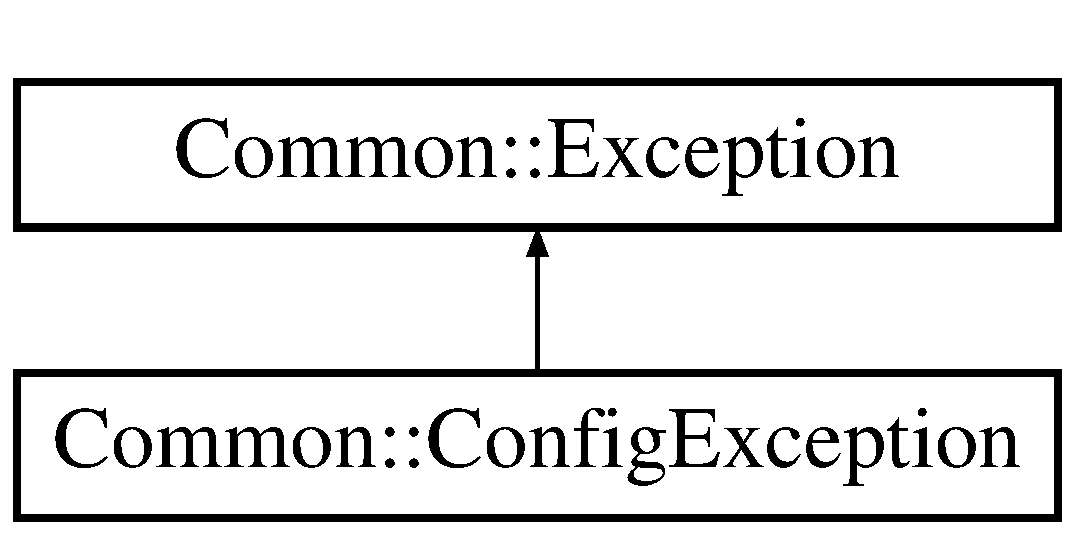
\includegraphics[height=2.000000cm]{class_common_1_1_config_exception}
\end{center}
\end{figure}
\subsection*{Public Member Functions}
\begin{DoxyCompactItemize}
\item 
\hyperlink{class_common_1_1_config_exception_a3b6738ec7ab3614f5b2e0d61d9316014}{Config\-Exception} (std\-::string const \&msg, std\-::string const \&obj\-Name=std\-::string())
\begin{DoxyCompactList}\small\item\em Constructor. \end{DoxyCompactList}\item 
void \hyperlink{class_common_1_1_config_exception_ad4ee85d0f156157abdde32b4fbf23369}{Display} (std\-::ostream \&os) const 
\begin{DoxyCompactList}\small\item\em Displays exception message on the given output stream. \end{DoxyCompactList}\item 
\hypertarget{class_common_1_1_config_exception_a1a340225bc9583bb9794e5ea8730020a}{void \hyperlink{class_common_1_1_config_exception_a1a340225bc9583bb9794e5ea8730020a}{Display} () const }\label{class_common_1_1_config_exception_a1a340225bc9583bb9794e5ea8730020a}

\begin{DoxyCompactList}\small\item\em Displays exception message on the standard error output. \end{DoxyCompactList}\item 
std\-::string \hyperlink{class_common_1_1_config_exception_a95f96a5d70b3a4ab3aa82f934bf74a7f}{Get\-Reason} () const 
\begin{DoxyCompactList}\small\item\em Returns a string containing the error message. \end{DoxyCompactList}\end{DoxyCompactItemize}
\subsection*{Additional Inherited Members}


\subsection{Detailed Description}
\hyperlink{class_common_1_1_config}{Config}, \hyperlink{class_common_1_1_config_reader}{Config\-Reader} and \hyperlink{class_common_1_1_config_map}{Config\-Map} exceptions. 

\begin{DoxyVersion}{Version}
1.\-0b 
\end{DoxyVersion}
\begin{DoxySince}{Since}
1.\-0b 
\end{DoxySince}
\begin{DoxyAuthor}{Author}
Noel De Martin, 2011 
\end{DoxyAuthor}


\subsection{Constructor \& Destructor Documentation}
\hypertarget{class_common_1_1_config_exception_a3b6738ec7ab3614f5b2e0d61d9316014}{\index{Common\-::\-Config\-Exception@{Common\-::\-Config\-Exception}!Config\-Exception@{Config\-Exception}}
\index{Config\-Exception@{Config\-Exception}!Common::ConfigException@{Common\-::\-Config\-Exception}}
\subsubsection[{Config\-Exception}]{\setlength{\rightskip}{0pt plus 5cm}Common\-::\-Config\-Exception\-::\-Config\-Exception (
\begin{DoxyParamCaption}
\item[{std\-::string const \&}]{msg, }
\item[{std\-::string const \&}]{obj\-Name = {\ttfamily std\-:\-:string~()}}
\end{DoxyParamCaption}
)\hspace{0.3cm}{\ttfamily [inline]}}}\label{class_common_1_1_config_exception_a3b6738ec7ab3614f5b2e0d61d9316014}


Constructor. 


\begin{DoxyParams}{Parameters}
{\em msg} & \hyperlink{class_common_1_1_exception}{Exception} message. \\
\hline
{\em obj\-Name} & Name of the object causing the exception, \char`\"{}\char`\"{} by default. \\
\hline
\end{DoxyParams}


\subsection{Member Function Documentation}
\hypertarget{class_common_1_1_config_exception_ad4ee85d0f156157abdde32b4fbf23369}{\index{Common\-::\-Config\-Exception@{Common\-::\-Config\-Exception}!Display@{Display}}
\index{Display@{Display}!Common::ConfigException@{Common\-::\-Config\-Exception}}
\subsubsection[{Display}]{\setlength{\rightskip}{0pt plus 5cm}void Common\-::\-Config\-Exception\-::\-Display (
\begin{DoxyParamCaption}
\item[{std\-::ostream \&}]{os}
\end{DoxyParamCaption}
) const\hspace{0.3cm}{\ttfamily [virtual]}}}\label{class_common_1_1_config_exception_ad4ee85d0f156157abdde32b4fbf23369}


Displays exception message on the given output stream. 


\begin{DoxyParams}{Parameters}
{\em os} & Output stream to display the message. \\
\hline
\end{DoxyParams}


Reimplemented from \hyperlink{class_common_1_1_exception_a2633eeaab3220268739977a04643a3cf}{Common\-::\-Exception}.

\hypertarget{class_common_1_1_config_exception_a95f96a5d70b3a4ab3aa82f934bf74a7f}{\index{Common\-::\-Config\-Exception@{Common\-::\-Config\-Exception}!Get\-Reason@{Get\-Reason}}
\index{Get\-Reason@{Get\-Reason}!Common::ConfigException@{Common\-::\-Config\-Exception}}
\subsubsection[{Get\-Reason}]{\setlength{\rightskip}{0pt plus 5cm}string Config\-Exception\-::\-Get\-Reason (
\begin{DoxyParamCaption}
{}
\end{DoxyParamCaption}
) const}}\label{class_common_1_1_config_exception_a95f96a5d70b3a4ab3aa82f934bf74a7f}


Returns a string containing the error message. 

\begin{DoxyReturn}{Returns}
String with the error. 
\end{DoxyReturn}


The documentation for this class was generated from the following files\-:\begin{DoxyCompactItemize}
\item 
Common/Config\-Exception.\-h\item 
Common/Config\-Exception.\-cpp\end{DoxyCompactItemize}

\hypertarget{class_common_1_1_config_helper}{\section{Common\-:\-:Config\-Helper Class Reference}
\label{class_common_1_1_config_helper}\index{Common\-::\-Config\-Helper@{Common\-::\-Config\-Helper}}
}


Static class that contains methods to manage \hyperlink{class_common_1_1_config}{Config} objects.  




{\ttfamily \#include $<$Config.\-h$>$}

\subsection*{Static Public Member Functions}
\begin{DoxyCompactItemize}
\item 
static \hyperlink{class_common_1_1_config}{Config} \hyperlink{class_common_1_1_config_helper_afa10958df84884f23c6141857805602d}{Read\-From\-File} (std\-::string const \&file\-Name)
\begin{DoxyCompactList}\small\item\em Returns a \hyperlink{class_common_1_1_config}{Config} object loaded from the given file. \end{DoxyCompactList}\end{DoxyCompactItemize}


\subsection{Detailed Description}
Static class that contains methods to manage \hyperlink{class_common_1_1_config}{Config} objects. 

\begin{DoxyVersion}{Version}
1.\-0b 
\end{DoxyVersion}
\begin{DoxySince}{Since}
1.\-0b 
\end{DoxySince}
\begin{DoxyAuthor}{Author}
Noel De Martin, 2011 
\end{DoxyAuthor}


\subsection{Member Function Documentation}
\hypertarget{class_common_1_1_config_helper_afa10958df84884f23c6141857805602d}{\index{Common\-::\-Config\-Helper@{Common\-::\-Config\-Helper}!Read\-From\-File@{Read\-From\-File}}
\index{Read\-From\-File@{Read\-From\-File}!Common::ConfigHelper@{Common\-::\-Config\-Helper}}
\subsubsection[{Read\-From\-File}]{\setlength{\rightskip}{0pt plus 5cm}static {\bf Config} Common\-::\-Config\-Helper\-::\-Read\-From\-File (
\begin{DoxyParamCaption}
\item[{std\-::string const \&}]{file\-Name}
\end{DoxyParamCaption}
)\hspace{0.3cm}{\ttfamily [inline]}, {\ttfamily [static]}}}\label{class_common_1_1_config_helper_afa10958df84884f23c6141857805602d}


Returns a \hyperlink{class_common_1_1_config}{Config} object loaded from the given file. 


\begin{DoxyExceptions}{Exceptions}
{\em \hyperlink{class_common_1_1_config_exception}{Config\-Exception}} & \\
\hline
\end{DoxyExceptions}


The documentation for this class was generated from the following file\-:\begin{DoxyCompactItemize}
\item 
Common/Config.\-h\end{DoxyCompactItemize}

\hypertarget{class_common_1_1_config_map}{\section{Common\-:\-:Config\-Map Class Reference}
\label{class_common_1_1_config_map}\index{Common\-::\-Config\-Map@{Common\-::\-Config\-Map}}
}


Contains and manages a collection of \hyperlink{class_common_1_1_config}{Config} objects.  




{\ttfamily \#include $<$Config\-Map.\-h$>$}

\subsection*{Classes}
\begin{DoxyCompactItemize}
\item 
class \hyperlink{class_common_1_1_config_map_1_1_iterator}{Iterator}
\begin{DoxyCompactList}\small\item\em Iterates over a \hyperlink{class_common_1_1_config_map}{Config\-Map} object. \end{DoxyCompactList}\end{DoxyCompactItemize}
\subsection*{Public Member Functions}
\begin{DoxyCompactItemize}
\item 
\hypertarget{class_common_1_1_config_map_ab77330842979d80d4e36ea9783b085e0}{\hyperlink{class_common_1_1_config_map_ab77330842979d80d4e36ea9783b085e0}{Config\-Map} ()}\label{class_common_1_1_config_map_ab77330842979d80d4e36ea9783b085e0}

\begin{DoxyCompactList}\small\item\em Constructor. \end{DoxyCompactList}\item 
bool \hyperlink{class_common_1_1_config_map_a4a68d6cba9ca84fa4702cdbd45faf487}{Add} (std\-::string const \&section, std\-::string const \&key, std\-::string const \&value)
\begin{DoxyCompactList}\small\item\em Adds a new value to the map. \end{DoxyCompactList}\item 
std\-::string const \& \hyperlink{class_common_1_1_config_map_a6fb312a35a095f2f9b1c1d171f8446d1}{Get\-Value} (std\-::string const \&section, std\-::string const \&key) const 
\begin{DoxyCompactList}\small\item\em Returns a requested value on the map. \end{DoxyCompactList}\item 
bool \hyperlink{class_common_1_1_config_map_a8bffcbff829a85af63db5189e37d0b66}{Contains} (std\-::string const \&section, std\-::string const \&key) const 
\begin{DoxyCompactList}\small\item\em Looks for the entry specified by the parameters of the function. \end{DoxyCompactList}\item 
\hypertarget{class_common_1_1_config_map_a1dbd03a3079d3b79d5c4107e963980e2}{int \hyperlink{class_common_1_1_config_map_a1dbd03a3079d3b79d5c4107e963980e2}{Get\-Size} () const }\label{class_common_1_1_config_map_a1dbd03a3079d3b79d5c4107e963980e2}

\begin{DoxyCompactList}\small\item\em Returns size of the map. \end{DoxyCompactList}\end{DoxyCompactItemize}
\subsection*{Friends}
\begin{DoxyCompactItemize}
\item 
\hypertarget{class_common_1_1_config_map_a9830fc407400559db7e7783cc10a9394}{class {\bfseries Iterator}}\label{class_common_1_1_config_map_a9830fc407400559db7e7783cc10a9394}

\end{DoxyCompactItemize}


\subsection{Detailed Description}
Contains and manages a collection of \hyperlink{class_common_1_1_config}{Config} objects. 

\begin{DoxyVersion}{Version}
1.\-0b 
\end{DoxyVersion}
\begin{DoxySince}{Since}
1.\-0b 
\end{DoxySince}
\begin{DoxyAuthor}{Author}
Ania Sikora, 2000 
\end{DoxyAuthor}


\subsection{Member Function Documentation}
\hypertarget{class_common_1_1_config_map_a4a68d6cba9ca84fa4702cdbd45faf487}{\index{Common\-::\-Config\-Map@{Common\-::\-Config\-Map}!Add@{Add}}
\index{Add@{Add}!Common::ConfigMap@{Common\-::\-Config\-Map}}
\subsubsection[{Add}]{\setlength{\rightskip}{0pt plus 5cm}bool Config\-Map\-::\-Add (
\begin{DoxyParamCaption}
\item[{std\-::string const \&}]{section, }
\item[{std\-::string const \&}]{key, }
\item[{std\-::string const \&}]{value}
\end{DoxyParamCaption}
)}}\label{class_common_1_1_config_map_a4a68d6cba9ca84fa4702cdbd45faf487}


Adds a new value to the map. 

If the entry already exists on the map returns false.


\begin{DoxyParams}{Parameters}
{\em section} & Section of the new entry. \\
\hline
{\em key} & Key of the new entry. \\
\hline
{\em value} & Value of the new entry.\\
\hline
\end{DoxyParams}
\begin{DoxyReturn}{Returns}
True if the insertion was successful, false otherwise. 
\end{DoxyReturn}
\hypertarget{class_common_1_1_config_map_a8bffcbff829a85af63db5189e37d0b66}{\index{Common\-::\-Config\-Map@{Common\-::\-Config\-Map}!Contains@{Contains}}
\index{Contains@{Contains}!Common::ConfigMap@{Common\-::\-Config\-Map}}
\subsubsection[{Contains}]{\setlength{\rightskip}{0pt plus 5cm}bool Config\-Map\-::\-Contains (
\begin{DoxyParamCaption}
\item[{std\-::string const \&}]{section, }
\item[{std\-::string const \&}]{key}
\end{DoxyParamCaption}
) const}}\label{class_common_1_1_config_map_a8bffcbff829a85af63db5189e37d0b66}


Looks for the entry specified by the parameters of the function. 


\begin{DoxyParams}{Parameters}
{\em section} & Section to find the entry. \\
\hline
{\em key} & Key to find the entry.\\
\hline
\end{DoxyParams}
\begin{DoxyReturn}{Returns}
True if the entry was found, false otherwise. 
\end{DoxyReturn}
\hypertarget{class_common_1_1_config_map_a6fb312a35a095f2f9b1c1d171f8446d1}{\index{Common\-::\-Config\-Map@{Common\-::\-Config\-Map}!Get\-Value@{Get\-Value}}
\index{Get\-Value@{Get\-Value}!Common::ConfigMap@{Common\-::\-Config\-Map}}
\subsubsection[{Get\-Value}]{\setlength{\rightskip}{0pt plus 5cm}string const \& Config\-Map\-::\-Get\-Value (
\begin{DoxyParamCaption}
\item[{std\-::string const \&}]{section, }
\item[{std\-::string const \&}]{key}
\end{DoxyParamCaption}
) const}}\label{class_common_1_1_config_map_a6fb312a35a095f2f9b1c1d171f8446d1}


Returns a requested value on the map. 


\begin{DoxyParams}{Parameters}
{\em section} & Section to find the value. \\
\hline
{\em key} & Key to find the value.\\
\hline
\end{DoxyParams}

\begin{DoxyExceptions}{Exceptions}
{\em \hyperlink{class_common_1_1_config_exception}{Config\-Exception}} & \\
\hline
\end{DoxyExceptions}


The documentation for this class was generated from the following files\-:\begin{DoxyCompactItemize}
\item 
Common/Config\-Map.\-h\item 
Common/Config\-Map.\-cpp\end{DoxyCompactItemize}

\hypertarget{class_common_1_1_config_reader}{\section{Common\-:\-:Config\-Reader Class Reference}
\label{class_common_1_1_config_reader}\index{Common\-::\-Config\-Reader@{Common\-::\-Config\-Reader}}
}


Abstract class, generates \hyperlink{class_common_1_1_config}{Config} objects from reading sources.  




{\ttfamily \#include $<$Config\-Reader.\-h$>$}

Inheritance diagram for Common\-:\-:Config\-Reader\-:\begin{figure}[H]
\begin{center}
\leavevmode
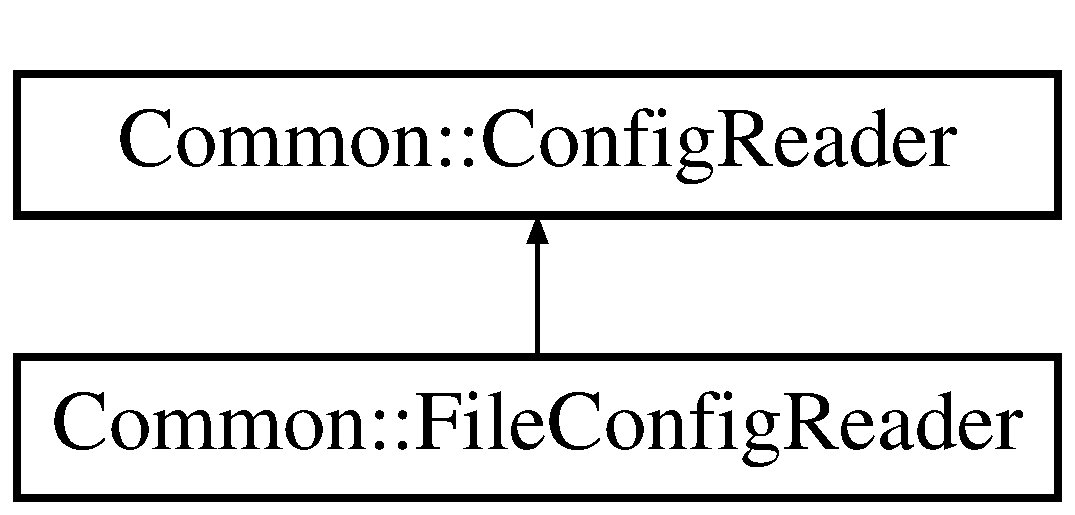
\includegraphics[height=2.000000cm]{class_common_1_1_config_reader}
\end{center}
\end{figure}
\subsection*{Public Member Functions}
\begin{DoxyCompactItemize}
\item 
\hypertarget{class_common_1_1_config_reader_a05f7bf0dca8d6cc11d7704936295c5c5}{\hyperlink{class_common_1_1_config_reader_a05f7bf0dca8d6cc11d7704936295c5c5}{Config\-Reader} ()}\label{class_common_1_1_config_reader_a05f7bf0dca8d6cc11d7704936295c5c5}

\begin{DoxyCompactList}\small\item\em Constructor. \end{DoxyCompactList}\item 
\hypertarget{class_common_1_1_config_reader_a261b278710c6b4de7e01a9eeae44f2c4}{virtual \hyperlink{class_common_1_1_config}{Config} {\bfseries Read} ()=0}\label{class_common_1_1_config_reader_a261b278710c6b4de7e01a9eeae44f2c4}

\end{DoxyCompactItemize}
\subsection*{Protected Member Functions}
\begin{DoxyCompactItemize}
\item 
\hypertarget{class_common_1_1_config_reader_aa7827a9e8b91a9052e02f4be96d0ef7a}{void \hyperlink{class_common_1_1_config_reader_aa7827a9e8b91a9052e02f4be96d0ef7a}{Analyze\-Line} (\hyperlink{class_common_1_1_config}{Config} \&config, std\-::string const \&line)}\label{class_common_1_1_config_reader_aa7827a9e8b91a9052e02f4be96d0ef7a}

\begin{DoxyCompactList}\small\item\em Loads the information of the line into the \hyperlink{class_common_1_1_config}{Config} object. \end{DoxyCompactList}\end{DoxyCompactItemize}


\subsection{Detailed Description}
Abstract class, generates \hyperlink{class_common_1_1_config}{Config} objects from reading sources. 

\begin{DoxyVersion}{Version}
1.\-0b 
\end{DoxyVersion}
\begin{DoxySince}{Since}
1.\-0b 
\end{DoxySince}
\begin{DoxyAuthor}{Author}
Ania Sikora, 2000 
\end{DoxyAuthor}


The documentation for this class was generated from the following files\-:\begin{DoxyCompactItemize}
\item 
Common/Config\-Reader.\-h\item 
Common/Config\-Reader.\-cpp\end{DoxyCompactItemize}

\hypertarget{class_controller}{\section{Controller Class Reference}
\label{class_controller}\index{Controller@{Controller}}
}


Provides the logic and controls the execution flow of the application.  




{\ttfamily \#include $<$Ctrl.\-h$>$}

\subsection*{Public Member Functions}
\begin{DoxyCompactItemize}
\item 
\hyperlink{class_controller_a43e23ba480023bc5066c0f80f8c964bd}{Controller} (\hyperlink{class_command_line}{Command\-Line} \&cmd\-Line)
\begin{DoxyCompactList}\small\item\em Constructor. \end{DoxyCompactList}\item 
\hypertarget{class_controller_a0ab87934c4f7a266cfdb86e0f36bc1b5}{\hyperlink{class_controller_a0ab87934c4f7a266cfdb86e0f36bc1b5}{$\sim$\-Controller} ()}\label{class_controller_a0ab87934c4f7a266cfdb86e0f36bc1b5}

\begin{DoxyCompactList}\small\item\em Destructor. \end{DoxyCompactList}\item 
void \hyperlink{class_controller_a17abb2cec6c0109e9b2df3cdc082eaad}{Run} ()
\begin{DoxyCompactList}\small\item\em Initializes all the necessary fields and starts the main loop of the A\-C. \end{DoxyCompactList}\item 
\hypertarget{class_controller_a4bb78bf21b480dce2e726c92ccc125f7}{void \hyperlink{class_controller_a4bb78bf21b480dce2e726c92ccc125f7}{Interrupt} ()}\label{class_controller_a4bb78bf21b480dce2e726c92ccc125f7}

\begin{DoxyCompactList}\small\item\em Sets the \-\_\-f\-Interrupted variable to 1. \end{DoxyCompactList}\item 
\hypertarget{class_controller_a89f48ed959f8719dab032cc0b7cd5718}{\hyperlink{class_controller_a89f48ed959f8719dab032cc0b7cd5718}{Controller} (\hyperlink{class_command_line}{Command\-Line} \&cmd\-Line, std\-::string const \&cfg\-File)}\label{class_controller_a89f48ed959f8719dab032cc0b7cd5718}

\begin{DoxyCompactList}\small\item\em Constructor, sets the command line for the user, determines the configuration for the application and prepares the system log. \end{DoxyCompactList}\item 
void \hyperlink{class_controller_a5b7edd9c004d719faa10d7ed0bfdc2b0}{Run} (\hyperlink{class_shut_down_manager}{Shut\-Down\-Manager} $\ast$sdm)
\begin{DoxyCompactList}\small\item\em Manages the execution flow of the application. The execution flow of analyzer is\-: \end{DoxyCompactList}\end{DoxyCompactItemize}


\subsection{Detailed Description}
Provides the logic and controls the execution flow of the application. 

Contains the main functionality of the A\-C, including its main loop which runs until all tuning operations have been finished.

\begin{DoxyVersion}{Version}
1.\-0 
\end{DoxyVersion}
\begin{DoxySince}{Since}
1.\-0 
\end{DoxySince}
\begin{DoxyAuthor}{Author}
Ania Sikora, 2002 
\end{DoxyAuthor}


\subsection{Constructor \& Destructor Documentation}
\hypertarget{class_controller_a43e23ba480023bc5066c0f80f8c964bd}{\index{Controller@{Controller}!Controller@{Controller}}
\index{Controller@{Controller}!Controller@{Controller}}
\subsubsection[{Controller}]{\setlength{\rightskip}{0pt plus 5cm}Controller\-::\-Controller (
\begin{DoxyParamCaption}
\item[{{\bf Command\-Line} \&}]{cmd\-Line}
\end{DoxyParamCaption}
)}}\label{class_controller_a43e23ba480023bc5066c0f80f8c964bd}


Constructor. 


\begin{DoxyParams}{Parameters}
{\em cmd\-Line} & Class that provides commandline communications with the user. \\
\hline
\end{DoxyParams}


\subsection{Member Function Documentation}
\hypertarget{class_controller_a5b7edd9c004d719faa10d7ed0bfdc2b0}{\index{Controller@{Controller}!Run@{Run}}
\index{Run@{Run}!Controller@{Controller}}
\subsubsection[{Run}]{\setlength{\rightskip}{0pt plus 5cm}void Controller\-::\-Run (
\begin{DoxyParamCaption}
\item[{{\bf Shut\-Down\-Manager} $\ast$}]{sdm}
\end{DoxyParamCaption}
)}}\label{class_controller_a5b7edd9c004d719faa10d7ed0bfdc2b0}


Manages the execution flow of the application. The execution flow of analyzer is\-: 


\begin{DoxyItemize}
\item create D\-T\-A\-P\-I, initialize collector, etc. 
\item create application model 
\item initialize all tunlets 
\item start application 
\item handle events 
\item destroy tunlets 
\item destroy app model 
\end{DoxyItemize}\hypertarget{class_controller_a17abb2cec6c0109e9b2df3cdc082eaad}{\index{Controller@{Controller}!Run@{Run}}
\index{Run@{Run}!Controller@{Controller}}
\subsubsection[{Run}]{\setlength{\rightskip}{0pt plus 5cm}void Controller\-::\-Run (
\begin{DoxyParamCaption}
{}
\end{DoxyParamCaption}
)}}\label{class_controller_a17abb2cec6c0109e9b2df3cdc082eaad}


Initializes all the necessary fields and starts the main loop of the A\-C. 

Creates a \hyperlink{class_task_manager}{Task\-Manager} objects and a Reactor and \hyperlink{class_p_t_p_acceptor}{P\-T\-P\-Acceptor} which will provide event handling and tuning capabilities. 

The documentation for this class was generated from the following files\-:\begin{DoxyCompactItemize}
\item 
A\-C/Ctrl.\-h\item 
Analyzer/Ctrl.\-h\item 
A\-C/Ctrl.\-cpp\item 
Analyzer/Ctrl.\-cpp\end{DoxyCompactItemize}

\hypertarget{class_common_1_1_counting_serializer}{\section{Common\-:\-:Counting\-Serializer Class Reference}
\label{class_common_1_1_counting_serializer}\index{Common\-::\-Counting\-Serializer@{Common\-::\-Counting\-Serializer}}
}


Stores the size of serialized data.  




{\ttfamily \#include $<$Net\-Ser.\-h$>$}

Inheritance diagram for Common\-:\-:Counting\-Serializer\-:\begin{figure}[H]
\begin{center}
\leavevmode
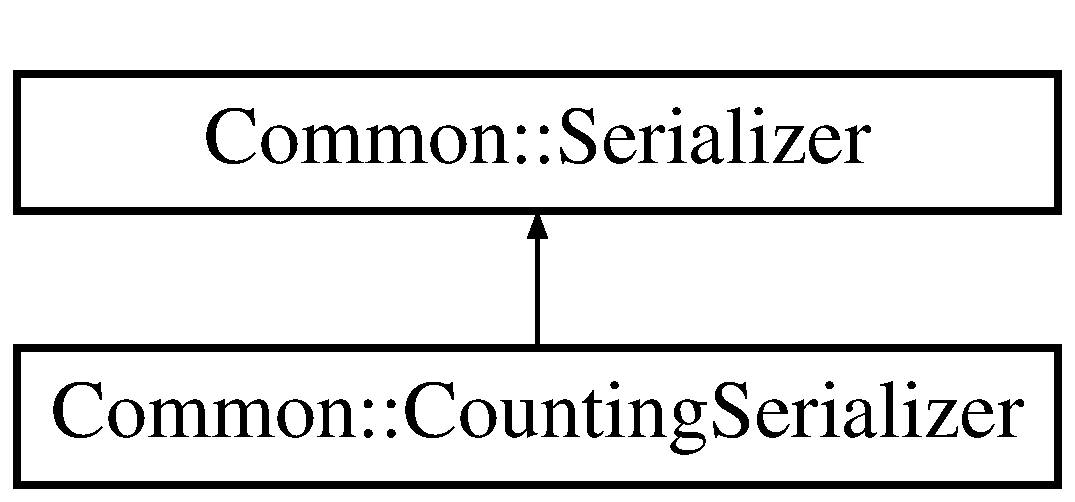
\includegraphics[height=2.000000cm]{class_common_1_1_counting_serializer}
\end{center}
\end{figure}
\subsection*{Public Member Functions}
\begin{DoxyCompactItemize}
\item 
\hypertarget{class_common_1_1_counting_serializer_a3bb6f8ba82a236ee5b2d7fc607c233f0}{\hyperlink{class_common_1_1_counting_serializer_a3bb6f8ba82a236ee5b2d7fc607c233f0}{Counting\-Serializer} ()}\label{class_common_1_1_counting_serializer_a3bb6f8ba82a236ee5b2d7fc607c233f0}

\begin{DoxyCompactList}\small\item\em Constructor. \end{DoxyCompactList}\item 
\hypertarget{class_common_1_1_counting_serializer_abc66a0949ecaaa9360362ea3953a0d28}{int\-\_\-t \hyperlink{class_common_1_1_counting_serializer_abc66a0949ecaaa9360362ea3953a0d28}{Get\-Size} () const }\label{class_common_1_1_counting_serializer_abc66a0949ecaaa9360362ea3953a0d28}

\begin{DoxyCompactList}\small\item\em Returns size of the serialized data. \end{DoxyCompactList}\item 
\hypertarget{class_common_1_1_counting_serializer_a3a145969a44e30ab60ee7812bbf45565}{void \hyperlink{class_common_1_1_counting_serializer_a3a145969a44e30ab60ee7812bbf45565}{Put\-Long} (long\-\_\-t l)}\label{class_common_1_1_counting_serializer_a3a145969a44e30ab60ee7812bbf45565}

\begin{DoxyCompactList}\small\item\em Adds the size of a serialized long. \end{DoxyCompactList}\item 
\hypertarget{class_common_1_1_counting_serializer_ab86f94e82c32e509e8ed1fe8e53340a8}{void \hyperlink{class_common_1_1_counting_serializer_ab86f94e82c32e509e8ed1fe8e53340a8}{Put\-Double} (double\-\_\-t d)}\label{class_common_1_1_counting_serializer_ab86f94e82c32e509e8ed1fe8e53340a8}

\begin{DoxyCompactList}\small\item\em Adds the size of a serialized double. \end{DoxyCompactList}\item 
\hypertarget{class_common_1_1_counting_serializer_a7a164188af395346b5de36a2f8e5b5ce}{void \hyperlink{class_common_1_1_counting_serializer_a7a164188af395346b5de36a2f8e5b5ce}{Put\-Bool} (bool\-\_\-t b)}\label{class_common_1_1_counting_serializer_a7a164188af395346b5de36a2f8e5b5ce}

\begin{DoxyCompactList}\small\item\em Adds the size of a serialized boolean. \end{DoxyCompactList}\item 
\hypertarget{class_common_1_1_counting_serializer_aba2cbeb047970aaf352362c279095490}{void \hyperlink{class_common_1_1_counting_serializer_aba2cbeb047970aaf352362c279095490}{Put\-Short} (short\-\_\-t s)}\label{class_common_1_1_counting_serializer_aba2cbeb047970aaf352362c279095490}

\begin{DoxyCompactList}\small\item\em Adds the size of a serialized short. \end{DoxyCompactList}\item 
\hypertarget{class_common_1_1_counting_serializer_a8f1bb6159f9369bd49818c15472e97bf}{void \hyperlink{class_common_1_1_counting_serializer_a8f1bb6159f9369bd49818c15472e97bf}{Put\-Byte} (byte\-\_\-t b)}\label{class_common_1_1_counting_serializer_a8f1bb6159f9369bd49818c15472e97bf}

\begin{DoxyCompactList}\small\item\em Adds the size of a serialized byte. \end{DoxyCompactList}\item 
\hypertarget{class_common_1_1_counting_serializer_a52bae0e495274ae83c344d2b1ce5efe9}{void \hyperlink{class_common_1_1_counting_serializer_a52bae0e495274ae83c344d2b1ce5efe9}{Put\-Char} (char\-\_\-t c)}\label{class_common_1_1_counting_serializer_a52bae0e495274ae83c344d2b1ce5efe9}

\begin{DoxyCompactList}\small\item\em Adds the size of a serialized char. \end{DoxyCompactList}\item 
\hypertarget{class_common_1_1_counting_serializer_a55e1c531bf83a8568c9ad07c23032c41}{void \hyperlink{class_common_1_1_counting_serializer_a55e1c531bf83a8568c9ad07c23032c41}{Put\-String} (std\-::string const \&str)}\label{class_common_1_1_counting_serializer_a55e1c531bf83a8568c9ad07c23032c41}

\begin{DoxyCompactList}\small\item\em Adds the size of a serialized string. \end{DoxyCompactList}\item 
\hypertarget{class_common_1_1_counting_serializer_aa5b2f108c3bfdf32681263d3dceedd6b}{void \hyperlink{class_common_1_1_counting_serializer_aa5b2f108c3bfdf32681263d3dceedd6b}{Put\-Int} (int\-\_\-t i)}\label{class_common_1_1_counting_serializer_aa5b2f108c3bfdf32681263d3dceedd6b}

\begin{DoxyCompactList}\small\item\em Adds the size of a serialized integer. \end{DoxyCompactList}\item 
\hypertarget{class_common_1_1_counting_serializer_a046147c02bb054da95faf8e287aa83de}{void \hyperlink{class_common_1_1_counting_serializer_a046147c02bb054da95faf8e287aa83de}{Put\-Buffer} (char const $\ast$buffer, int buffer\-Size)}\label{class_common_1_1_counting_serializer_a046147c02bb054da95faf8e287aa83de}

\begin{DoxyCompactList}\small\item\em Adds the size of a serialized buffer. \end{DoxyCompactList}\end{DoxyCompactItemize}


\subsection{Detailed Description}
Stores the size of serialized data. 

\begin{DoxyVersion}{Version}
1.\-0b 
\end{DoxyVersion}
\begin{DoxySince}{Since}
1.\-0b 
\end{DoxySince}
\begin{DoxyAuthor}{Author}
Ania Sikora, 2002 
\end{DoxyAuthor}


The documentation for this class was generated from the following file\-:\begin{DoxyCompactItemize}
\item 
Common/Net\-Ser.\-h\end{DoxyCompactItemize}

\hypertarget{structcur_state}{\section{cur\-State Class Reference}
\label{structcur_state}\index{cur\-State@{cur\-State}}
}


Struct that stores the iteration, batch and number of tuples.  


\subsection*{Public Attributes}
\begin{DoxyCompactItemize}
\item 
\hypertarget{structcur_state_a52f0ae3f978cdf1eb66ef02d1b223e62}{int {\bfseries iter}}\label{structcur_state_a52f0ae3f978cdf1eb66ef02d1b223e62}

\item 
\hypertarget{structcur_state_a9fbda04627b62cc569eb75980d1afecc}{int {\bfseries batch}}\label{structcur_state_a9fbda04627b62cc569eb75980d1afecc}

\item 
\hypertarget{structcur_state_a75c3cd911a5d911cf0c540afe4c406fe}{int {\bfseries num\-Tuples}}\label{structcur_state_a75c3cd911a5d911cf0c540afe4c406fe}

\end{DoxyCompactItemize}


\subsection{Detailed Description}
Struct that stores the iteration, batch and number of tuples. 

The documentation for this class was generated from the following file\-:\begin{DoxyCompactItemize}
\item 
Analyzer/Factoring\-Tunlet\-\_\-nw.\-cpp\end{DoxyCompactItemize}

\hypertarget{class_common_1_1_date_time}{\section{Common\-:\-:Date\-Time Class Reference}
\label{class_common_1_1_date_time}\index{Common\-::\-Date\-Time@{Common\-::\-Date\-Time}}
}


Holds a timestamp.  




{\ttfamily \#include $<$Date\-Time.\-h$>$}

\subsection*{Public Member Functions}
\begin{DoxyCompactItemize}
\item 
\hypertarget{class_common_1_1_date_time_a3ccfb87f7a2e9683b91964e32d907161}{\hyperlink{class_common_1_1_date_time_a3ccfb87f7a2e9683b91964e32d907161}{Date\-Time} ()}\label{class_common_1_1_date_time_a3ccfb87f7a2e9683b91964e32d907161}

\begin{DoxyCompactList}\small\item\em Constructor, sets the current date and time. \end{DoxyCompactList}\item 
\hypertarget{class_common_1_1_date_time_aba159de639cf43c4191110eb6e5bba25}{int \hyperlink{class_common_1_1_date_time_aba159de639cf43c4191110eb6e5bba25}{Get\-Year} () const }\label{class_common_1_1_date_time_aba159de639cf43c4191110eb6e5bba25}

\begin{DoxyCompactList}\small\item\em Returns year represented by this date. \end{DoxyCompactList}\item 
\hypertarget{class_common_1_1_date_time_abf791831b6d7be2d505425e03b802c9c}{int \hyperlink{class_common_1_1_date_time_abf791831b6d7be2d505425e03b802c9c}{Get\-Month} () const }\label{class_common_1_1_date_time_abf791831b6d7be2d505425e03b802c9c}

\begin{DoxyCompactList}\small\item\em Returns month represented by this date. \end{DoxyCompactList}\item 
\hypertarget{class_common_1_1_date_time_a5cf339c1158f5f95bff6e7c2f556c057}{int \hyperlink{class_common_1_1_date_time_a5cf339c1158f5f95bff6e7c2f556c057}{Get\-Day} () const }\label{class_common_1_1_date_time_a5cf339c1158f5f95bff6e7c2f556c057}

\begin{DoxyCompactList}\small\item\em Returns day represented by this date. \end{DoxyCompactList}\item 
\hypertarget{class_common_1_1_date_time_a3b2d1fd6273d9d657ae2d0f8d265c063}{int \hyperlink{class_common_1_1_date_time_a3b2d1fd6273d9d657ae2d0f8d265c063}{Get\-Hour} () const }\label{class_common_1_1_date_time_a3b2d1fd6273d9d657ae2d0f8d265c063}

\begin{DoxyCompactList}\small\item\em Returns hour represented by this date. \end{DoxyCompactList}\item 
\hypertarget{class_common_1_1_date_time_a58a17b09e909d30b271567ba09629143}{int \hyperlink{class_common_1_1_date_time_a58a17b09e909d30b271567ba09629143}{Get\-Minute} () const }\label{class_common_1_1_date_time_a58a17b09e909d30b271567ba09629143}

\begin{DoxyCompactList}\small\item\em Returns minute represented by this date. \end{DoxyCompactList}\item 
\hypertarget{class_common_1_1_date_time_aad38f0369fe0a0c1d4a711ce6dee6af6}{int \hyperlink{class_common_1_1_date_time_aad38f0369fe0a0c1d4a711ce6dee6af6}{Get\-Second} () const }\label{class_common_1_1_date_time_aad38f0369fe0a0c1d4a711ce6dee6af6}

\begin{DoxyCompactList}\small\item\em Returns second represented by this date. \end{DoxyCompactList}\item 
std\-::string \hyperlink{class_common_1_1_date_time_a3b10dedb9400b0c03fec33fdb8ec3c9a}{Get\-String\-Value} () const 
\begin{DoxyCompactList}\small\item\em Returns a string with the date. \end{DoxyCompactList}\end{DoxyCompactItemize}


\subsection{Detailed Description}
Holds a timestamp. 

\begin{DoxyVersion}{Version}
1.\-0 
\end{DoxyVersion}
\begin{DoxySince}{Since}
1.\-0 
\end{DoxySince}
\begin{DoxyAuthor}{Author}
Ania Sikora, 2001 
\end{DoxyAuthor}


\subsection{Member Function Documentation}
\hypertarget{class_common_1_1_date_time_a3b10dedb9400b0c03fec33fdb8ec3c9a}{\index{Common\-::\-Date\-Time@{Common\-::\-Date\-Time}!Get\-String\-Value@{Get\-String\-Value}}
\index{Get\-String\-Value@{Get\-String\-Value}!Common::DateTime@{Common\-::\-Date\-Time}}
\subsubsection[{Get\-String\-Value}]{\setlength{\rightskip}{0pt plus 5cm}string Date\-Time\-::\-Get\-String\-Value (
\begin{DoxyParamCaption}
{}
\end{DoxyParamCaption}
) const}}\label{class_common_1_1_date_time_a3b10dedb9400b0c03fec33fdb8ec3c9a}


Returns a string with the date. 

The format of the returned string is \char`\"{}dd.\-mm.\-yyyy hh\-:\-M\-M\-:ss\char`\"{}. 

The documentation for this class was generated from the following files\-:\begin{DoxyCompactItemize}
\item 
Common/Date\-Time.\-h\item 
Common/Date\-Time.\-cpp\end{DoxyCompactItemize}

\hypertarget{class_common_1_1_de_serializer}{\section{Common\-:\-:De\-Serializer Class Reference}
\label{class_common_1_1_de_serializer}\index{Common\-::\-De\-Serializer@{Common\-::\-De\-Serializer}}
}


Abstract class, recovers serialized data from a stream.  




{\ttfamily \#include $<$Serial.\-h$>$}

Inheritance diagram for Common\-:\-:De\-Serializer\-:\begin{figure}[H]
\begin{center}
\leavevmode
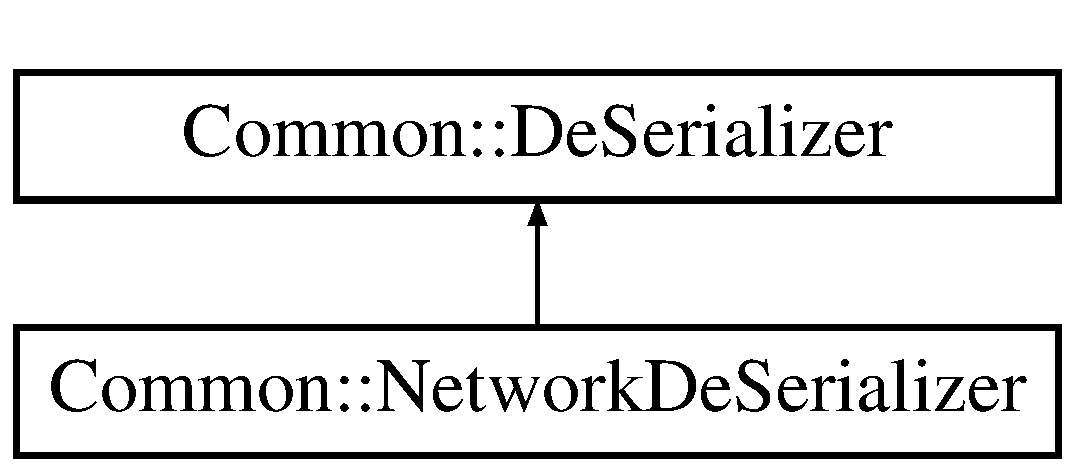
\includegraphics[height=2.000000cm]{class_common_1_1_de_serializer}
\end{center}
\end{figure}
\subsection*{Public Member Functions}
\begin{DoxyCompactItemize}
\item 
\hypertarget{class_common_1_1_de_serializer_aa2fff1fe5df35908ddcc262f2dc405ac}{virtual byte\-\_\-t \hyperlink{class_common_1_1_de_serializer_aa2fff1fe5df35908ddcc262f2dc405ac}{Get\-Byte} ()=0}\label{class_common_1_1_de_serializer_aa2fff1fe5df35908ddcc262f2dc405ac}

\begin{DoxyCompactList}\small\item\em Reads byte value from the stream. \end{DoxyCompactList}\item 
\hypertarget{class_common_1_1_de_serializer_aafef2f1bc360ca768e2d11dabe6a49e5}{virtual char\-\_\-t \hyperlink{class_common_1_1_de_serializer_aafef2f1bc360ca768e2d11dabe6a49e5}{Get\-Char} ()=0}\label{class_common_1_1_de_serializer_aafef2f1bc360ca768e2d11dabe6a49e5}

\begin{DoxyCompactList}\small\item\em Reads char value from the stream. \end{DoxyCompactList}\item 
\hypertarget{class_common_1_1_de_serializer_ad16f227270021a4db8a05bfd3f1b63bf}{virtual bool\-\_\-t \hyperlink{class_common_1_1_de_serializer_ad16f227270021a4db8a05bfd3f1b63bf}{Get\-Bool} ()=0}\label{class_common_1_1_de_serializer_ad16f227270021a4db8a05bfd3f1b63bf}

\begin{DoxyCompactList}\small\item\em Reads bool value from the stream. \end{DoxyCompactList}\item 
\hypertarget{class_common_1_1_de_serializer_ab6b26aa11a37f0e75becccddcc67dbdf}{virtual short\-\_\-t \hyperlink{class_common_1_1_de_serializer_ab6b26aa11a37f0e75becccddcc67dbdf}{Get\-Short} ()=0}\label{class_common_1_1_de_serializer_ab6b26aa11a37f0e75becccddcc67dbdf}

\begin{DoxyCompactList}\small\item\em Reads short value from the stream. \end{DoxyCompactList}\item 
\hypertarget{class_common_1_1_de_serializer_accf0be5bb4c6ae60c15d912863437789}{virtual int\-\_\-t \hyperlink{class_common_1_1_de_serializer_accf0be5bb4c6ae60c15d912863437789}{Get\-Int} ()=0}\label{class_common_1_1_de_serializer_accf0be5bb4c6ae60c15d912863437789}

\begin{DoxyCompactList}\small\item\em Reads int value from the stream. \end{DoxyCompactList}\item 
\hypertarget{class_common_1_1_de_serializer_a1c869a74ee3d1106a26a425448192563}{virtual long\-\_\-t \hyperlink{class_common_1_1_de_serializer_a1c869a74ee3d1106a26a425448192563}{Get\-Long} ()=0}\label{class_common_1_1_de_serializer_a1c869a74ee3d1106a26a425448192563}

\begin{DoxyCompactList}\small\item\em Reads long value from the stream. \end{DoxyCompactList}\item 
\hypertarget{class_common_1_1_de_serializer_adda6f9a260dcd3f0c925799448364b70}{virtual double\-\_\-t \hyperlink{class_common_1_1_de_serializer_adda6f9a260dcd3f0c925799448364b70}{Get\-Double} ()=0}\label{class_common_1_1_de_serializer_adda6f9a260dcd3f0c925799448364b70}

\begin{DoxyCompactList}\small\item\em Reads double value from the stream. \end{DoxyCompactList}\item 
\hypertarget{class_common_1_1_de_serializer_adbee4f2d29abe1ab78e16d5c30afe8dd}{virtual std\-::string \hyperlink{class_common_1_1_de_serializer_adbee4f2d29abe1ab78e16d5c30afe8dd}{Get\-String} ()=0}\label{class_common_1_1_de_serializer_adbee4f2d29abe1ab78e16d5c30afe8dd}

\begin{DoxyCompactList}\small\item\em Reads string value from the stream. \end{DoxyCompactList}\item 
\hypertarget{class_common_1_1_de_serializer_a6659c1a1cf712983d088931be967f284}{virtual void \hyperlink{class_common_1_1_de_serializer_a6659c1a1cf712983d088931be967f284}{Get\-Buffer} (char $\ast$buffer, int buffer\-Size)=0}\label{class_common_1_1_de_serializer_a6659c1a1cf712983d088931be967f284}

\begin{DoxyCompactList}\small\item\em Reads data directly from the stream. \end{DoxyCompactList}\end{DoxyCompactItemize}


\subsection{Detailed Description}
Abstract class, recovers serialized data from a stream. 

\begin{DoxyVersion}{Version}
1.\-0b 
\end{DoxyVersion}
\begin{DoxySince}{Since}
1.\-0b 
\end{DoxySince}
\begin{DoxyAuthor}{Author}
Ania Sikora, 2002 
\end{DoxyAuthor}


The documentation for this class was generated from the following file\-:\begin{DoxyCompactItemize}
\item 
Common/Serial.\-h\end{DoxyCompactItemize}

\hypertarget{class_di_ex}{\section{Di\-Ex Class Reference}
\label{class_di_ex}\index{Di\-Ex@{Di\-Ex}}
}


Implements the Dyninst's Exceptions.  




{\ttfamily \#include $<$di.\-h$>$}

\subsection*{Public Member Functions}
\begin{DoxyCompactItemize}
\item 
\hypertarget{class_di_ex_ab71373ff998e8179b17ca65be0aee491}{{\bfseries \-\_\-obj\-Name} (obj\-Name)}\label{class_di_ex_ab71373ff998e8179b17ca65be0aee491}

\item 
string const \& \hyperlink{class_di_ex_a977a9ac4395817363e569f1016fb8340}{Get\-Message} () const 
\begin{DoxyCompactList}\small\item\em Exception message getter. \end{DoxyCompactList}\item 
string const \& \hyperlink{class_di_ex_ae1b98e1e8b577f168deaea6852a7139b}{Get\-Object\-Name} () const 
\begin{DoxyCompactList}\small\item\em Object Name getter. \end{DoxyCompactList}\end{DoxyCompactItemize}
\subsection*{Public Attributes}
\begin{DoxyCompactItemize}
\item 
\hyperlink{class_di_ex_ad80ae482a21daa73f24fcc9c5911523f}{\-\_\-\-\_\-pad0\-\_\-\-\_\-}\-: \-\_\-msg (msg)
\begin{DoxyCompactList}\small\item\em Constructor. \end{DoxyCompactList}\end{DoxyCompactItemize}


\subsection{Detailed Description}
Implements the Dyninst's Exceptions. 

\begin{DoxyVersion}{Version}
1.\-0b 
\end{DoxyVersion}
\begin{DoxyAuthor}{Author}
Ania Sikora, 2002 
\end{DoxyAuthor}
\begin{DoxySince}{Since}
1.\-0b 
\end{DoxySince}


\subsection{Member Function Documentation}
\hypertarget{class_di_ex_a977a9ac4395817363e569f1016fb8340}{\index{Di\-Ex@{Di\-Ex}!Get\-Message@{Get\-Message}}
\index{Get\-Message@{Get\-Message}!DiEx@{Di\-Ex}}
\subsubsection[{Get\-Message}]{\setlength{\rightskip}{0pt plus 5cm}string const\& Di\-Ex\-::\-Get\-Message (
\begin{DoxyParamCaption}
{}
\end{DoxyParamCaption}
) const\hspace{0.3cm}{\ttfamily [inline]}}}\label{class_di_ex_a977a9ac4395817363e569f1016fb8340}


Exception message getter. 

\begin{DoxyReturn}{Returns}
\-\_\-msg 
\end{DoxyReturn}
\hypertarget{class_di_ex_ae1b98e1e8b577f168deaea6852a7139b}{\index{Di\-Ex@{Di\-Ex}!Get\-Object\-Name@{Get\-Object\-Name}}
\index{Get\-Object\-Name@{Get\-Object\-Name}!DiEx@{Di\-Ex}}
\subsubsection[{Get\-Object\-Name}]{\setlength{\rightskip}{0pt plus 5cm}string const\& Di\-Ex\-::\-Get\-Object\-Name (
\begin{DoxyParamCaption}
{}
\end{DoxyParamCaption}
) const\hspace{0.3cm}{\ttfamily [inline]}}}\label{class_di_ex_ae1b98e1e8b577f168deaea6852a7139b}


Object Name getter. 

\begin{DoxyReturn}{Returns}
\-\_\-obj\-Name 
\end{DoxyReturn}


\subsection{Member Data Documentation}
\hypertarget{class_di_ex_ad80ae482a21daa73f24fcc9c5911523f}{\index{Di\-Ex@{Di\-Ex}!\-\_\-\-\_\-pad0\-\_\-\-\_\-@{\-\_\-\-\_\-pad0\-\_\-\-\_\-}}
\index{\-\_\-\-\_\-pad0\-\_\-\-\_\-@{\-\_\-\-\_\-pad0\-\_\-\-\_\-}!DiEx@{Di\-Ex}}
\subsubsection[{\-\_\-\-\_\-pad0\-\_\-\-\_\-}]{\setlength{\rightskip}{0pt plus 5cm}Di\-Ex\-::\-\_\-\-\_\-pad0\-\_\-\-\_\-}}\label{class_di_ex_ad80ae482a21daa73f24fcc9c5911523f}


Constructor. 


\begin{DoxyParams}{Parameters}
{\em msg} & Exception message to display \\
\hline
{\em obj\-Name} & Object Name \\
\hline
\end{DoxyParams}


The documentation for this class was generated from the following file\-:\begin{DoxyCompactItemize}
\item 
Common/di.\-h\end{DoxyCompactItemize}

\hypertarget{class_di_function}{\section{Di\-Function Class Reference}
\label{class_di_function}\index{Di\-Function@{Di\-Function}}
}


Dyninst's function class. It represents a function in the application.  




{\ttfamily \#include $<$di.\-h$>$}

\subsection*{Public Member Functions}
\begin{DoxyCompactItemize}
\item 
\hypertarget{class_di_function_adeec90e7f3aff80b77c451cddc47941f}{{\bfseries Di\-Function} (B\-Patch\-\_\-image \&bp\-Image, string const \&func\-Name)}\label{class_di_function_adeec90e7f3aff80b77c451cddc47941f}

\item 
void \hyperlink{class_di_function_a0f72a27e659c6593d7b514507265dec8}{Get\-Line\-Number} (unsigned int \&start, unsigned int \&end, char $\ast$file\-Name, unsigned int \&max)
\begin{DoxyCompactList}\small\item\em Gets the current line number and the file name. \end{DoxyCompactList}\item 
unsigned long \hyperlink{class_di_function_a84996228fdec848ff14b1b3f04cedcb3}{Get\-Address} ()
\begin{DoxyCompactList}\small\item\em Reads the address of \-\_\-bp\-Var. \end{DoxyCompactList}\item 
char const $\ast$ \hyperlink{class_di_function_a8fe2de104488ec6714cd44614b79e3ca}{Get\-Params} ()
\begin{DoxyCompactList}\small\item\em Gets the parameters of \-\_\-bp\-Func. \end{DoxyCompactList}\item 
Point\-Vector $\ast$ \hyperlink{class_di_function_aabc45084deadfa69588048023e538840}{Find\-Point} (B\-Patch\-\_\-procedure\-Location loc=B\-Patch\-\_\-subroutine)
\begin{DoxyCompactList}\small\item\em Finds the procedure point for the given location. \end{DoxyCompactList}\item 
void \hyperlink{class_di_function_a4c471073fa7f0f0d313ff2fee7b6d988}{Get\-Name} (char $\ast$file\-Name, int len)
\begin{DoxyCompactList}\small\item\em Getter of the file name. \end{DoxyCompactList}\item 
\hypertarget{class_di_function_a7ea5b551ae1e57d98e617ba8ba3ddc3c}{{\bfseries operator B\-Patch\-\_\-function \&} ()}\label{class_di_function_a7ea5b551ae1e57d98e617ba8ba3ddc3c}

\end{DoxyCompactItemize}
\subsection*{Static Public Member Functions}
\begin{DoxyCompactItemize}
\item 
static void \hyperlink{class_di_function_a0b3e0e96d8f5a35a0cf053d1c46ad31a}{Dump} (Func\-Vector \&fv)
\begin{DoxyCompactList}\small\item\em Prints all functions from the Func\-Vector {\itshape fv} \end{DoxyCompactList}\end{DoxyCompactItemize}


\subsection{Detailed Description}
Dyninst's function class. It represents a function in the application. 

\begin{DoxyVersion}{Version}
1.\-0b 
\end{DoxyVersion}
\begin{DoxyAuthor}{Author}
Ania Sikora, 2002 
\end{DoxyAuthor}
\begin{DoxySince}{Since}
1.\-0b 
\end{DoxySince}


\subsection{Member Function Documentation}
\hypertarget{class_di_function_a0b3e0e96d8f5a35a0cf053d1c46ad31a}{\index{Di\-Function@{Di\-Function}!Dump@{Dump}}
\index{Dump@{Dump}!DiFunction@{Di\-Function}}
\subsubsection[{Dump}]{\setlength{\rightskip}{0pt plus 5cm}void Di\-Function\-::\-Dump (
\begin{DoxyParamCaption}
\item[{Di\-Function\-::\-Func\-Vector \&}]{fv}
\end{DoxyParamCaption}
)\hspace{0.3cm}{\ttfamily [static]}}}\label{class_di_function_a0b3e0e96d8f5a35a0cf053d1c46ad31a}


Prints all functions from the Func\-Vector {\itshape fv} 


\begin{DoxyParams}{Parameters}
{\em fv} & Func\-Vector \\
\hline
\end{DoxyParams}
\hypertarget{class_di_function_aabc45084deadfa69588048023e538840}{\index{Di\-Function@{Di\-Function}!Find\-Point@{Find\-Point}}
\index{Find\-Point@{Find\-Point}!DiFunction@{Di\-Function}}
\subsubsection[{Find\-Point}]{\setlength{\rightskip}{0pt plus 5cm}Di\-Function\-::\-Point\-Vector $\ast$ Di\-Function\-::\-Find\-Point (
\begin{DoxyParamCaption}
\item[{B\-Patch\-\_\-procedure\-Location}]{loc = {\ttfamily BPatch\-\_\-subroutine}}
\end{DoxyParamCaption}
)}}\label{class_di_function_aabc45084deadfa69588048023e538840}


Finds the procedure point for the given location. 


\begin{DoxyParams}{Parameters}
{\em loc} & Location of the point to look for \\
\hline
\end{DoxyParams}
\begin{DoxyReturn}{Returns}
Point Vector of the specified location 
\end{DoxyReturn}
\hypertarget{class_di_function_a84996228fdec848ff14b1b3f04cedcb3}{\index{Di\-Function@{Di\-Function}!Get\-Address@{Get\-Address}}
\index{Get\-Address@{Get\-Address}!DiFunction@{Di\-Function}}
\subsubsection[{Get\-Address}]{\setlength{\rightskip}{0pt plus 5cm}unsigned long Di\-Function\-::\-Get\-Address (
\begin{DoxyParamCaption}
{}
\end{DoxyParamCaption}
)}}\label{class_di_function_a84996228fdec848ff14b1b3f04cedcb3}


Reads the address of \-\_\-bp\-Var. 

\begin{DoxyReturn}{Returns}
Address of \-\_\-bp\-Var 
\end{DoxyReturn}
\hypertarget{class_di_function_a0f72a27e659c6593d7b514507265dec8}{\index{Di\-Function@{Di\-Function}!Get\-Line\-Number@{Get\-Line\-Number}}
\index{Get\-Line\-Number@{Get\-Line\-Number}!DiFunction@{Di\-Function}}
\subsubsection[{Get\-Line\-Number}]{\setlength{\rightskip}{0pt plus 5cm}void Di\-Function\-::\-Get\-Line\-Number (
\begin{DoxyParamCaption}
\item[{unsigned int \&}]{start, }
\item[{unsigned int \&}]{end, }
\item[{char $\ast$}]{file\-Name, }
\item[{unsigned int \&}]{max}
\end{DoxyParamCaption}
)}}\label{class_di_function_a0f72a27e659c6593d7b514507265dec8}


Gets the current line number and the file name. 


\begin{DoxyParams}{Parameters}
{\em start} & Address \\
\hline
{\em end} & Line \\
\hline
{\em file\-Name} & String where the file name will be saved \\
\hline
{\em max} & Length \\
\hline
\end{DoxyParams}
\hypertarget{class_di_function_a4c471073fa7f0f0d313ff2fee7b6d988}{\index{Di\-Function@{Di\-Function}!Get\-Name@{Get\-Name}}
\index{Get\-Name@{Get\-Name}!DiFunction@{Di\-Function}}
\subsubsection[{Get\-Name}]{\setlength{\rightskip}{0pt plus 5cm}void Di\-Function\-::\-Get\-Name (
\begin{DoxyParamCaption}
\item[{char $\ast$}]{file\-Name, }
\item[{int}]{len}
\end{DoxyParamCaption}
)}}\label{class_di_function_a4c471073fa7f0f0d313ff2fee7b6d988}


Getter of the file name. 


\begin{DoxyParams}{Parameters}
{\em file\-Name} & Parameter where the file name will be stored \\
\hline
{\em len} & max length of the file name \\
\hline
\end{DoxyParams}
\hypertarget{class_di_function_a8fe2de104488ec6714cd44614b79e3ca}{\index{Di\-Function@{Di\-Function}!Get\-Params@{Get\-Params}}
\index{Get\-Params@{Get\-Params}!DiFunction@{Di\-Function}}
\subsubsection[{Get\-Params}]{\setlength{\rightskip}{0pt plus 5cm}char const $\ast$ Di\-Function\-::\-Get\-Params (
\begin{DoxyParamCaption}
{}
\end{DoxyParamCaption}
)}}\label{class_di_function_a8fe2de104488ec6714cd44614b79e3ca}


Gets the parameters of \-\_\-bp\-Func. 

\begin{DoxyReturn}{Returns}
Parameters of the current function 
\end{DoxyReturn}


The documentation for this class was generated from the following files\-:\begin{DoxyCompactItemize}
\item 
Common/di.\-h\item 
Common/di.\-cpp\end{DoxyCompactItemize}

\hypertarget{class_di_image}{\section{Di\-Image Class Reference}
\label{class_di_image}\index{Di\-Image@{Di\-Image}}
}


Reads the program's image and gets an associated image object (the executable associated with a thread). It can also find a variable in the image and return it.  




{\ttfamily \#include $<$di.\-h$>$}

\subsection*{Public Member Functions}
\begin{DoxyCompactItemize}
\item 
\hypertarget{class_di_image_afd1a854b23db70ddf7f25c82e60102a2}{{\bfseries Di\-Image} (B\-Patch\-\_\-process \&bp\-Process)}\label{class_di_image_afd1a854b23db70ddf7f25c82e60102a2}

\item 
B\-Patch\-\_\-variable\-Expr $\ast$ \hyperlink{class_di_image_a1442d33b97ad72a1ddd6aa4a7e9db916}{Find\-Variable} (const char $\ast$name)
\begin{DoxyCompactList}\small\item\em Finds the variable from \-\_\-bp\-Image via name and returns it. \end{DoxyCompactList}\item 
\hypertarget{class_di_image_a2dd2df8fbb5a872bb79132d57df858ef}{{\bfseries operator B\-Patch\-\_\-image \&} ()}\label{class_di_image_a2dd2df8fbb5a872bb79132d57df858ef}

\end{DoxyCompactItemize}


\subsection{Detailed Description}
Reads the program's image and gets an associated image object (the executable associated with a thread). It can also find a variable in the image and return it. 

\begin{DoxyVersion}{Version}
1.\-0b 
\end{DoxyVersion}
\begin{DoxyAuthor}{Author}
Ania Sikora, 2002 
\end{DoxyAuthor}
\begin{DoxySince}{Since}
1.\-0b 
\end{DoxySince}


\subsection{Member Function Documentation}
\hypertarget{class_di_image_a1442d33b97ad72a1ddd6aa4a7e9db916}{\index{Di\-Image@{Di\-Image}!Find\-Variable@{Find\-Variable}}
\index{Find\-Variable@{Find\-Variable}!DiImage@{Di\-Image}}
\subsubsection[{Find\-Variable}]{\setlength{\rightskip}{0pt plus 5cm}B\-Patch\-\_\-variable\-Expr $\ast$ Di\-Image\-::\-Find\-Variable (
\begin{DoxyParamCaption}
\item[{const char $\ast$}]{name}
\end{DoxyParamCaption}
)}}\label{class_di_image_a1442d33b97ad72a1ddd6aa4a7e9db916}


Finds the variable from \-\_\-bp\-Image via name and returns it. 


\begin{DoxyParams}{Parameters}
{\em name} & Name of the variable \\
\hline
\end{DoxyParams}
\begin{DoxyReturn}{Returns}
Global variable matching $<$name$>$ in the image. N\-U\-L\-L if not found. 
\end{DoxyReturn}


The documentation for this class was generated from the following files\-:\begin{DoxyCompactItemize}
\item 
Common/di.\-h\item 
Common/di.\-cpp\end{DoxyCompactItemize}

\hypertarget{class_di_int_type}{\section{Di\-Int\-Type Class Reference}
\label{class_di_int_type}\index{Di\-Int\-Type@{Di\-Int\-Type}}
}


Dyninst Int type class.  




{\ttfamily \#include $<$di.\-h$>$}

Inheritance diagram for Di\-Int\-Type\-:\begin{figure}[H]
\begin{center}
\leavevmode
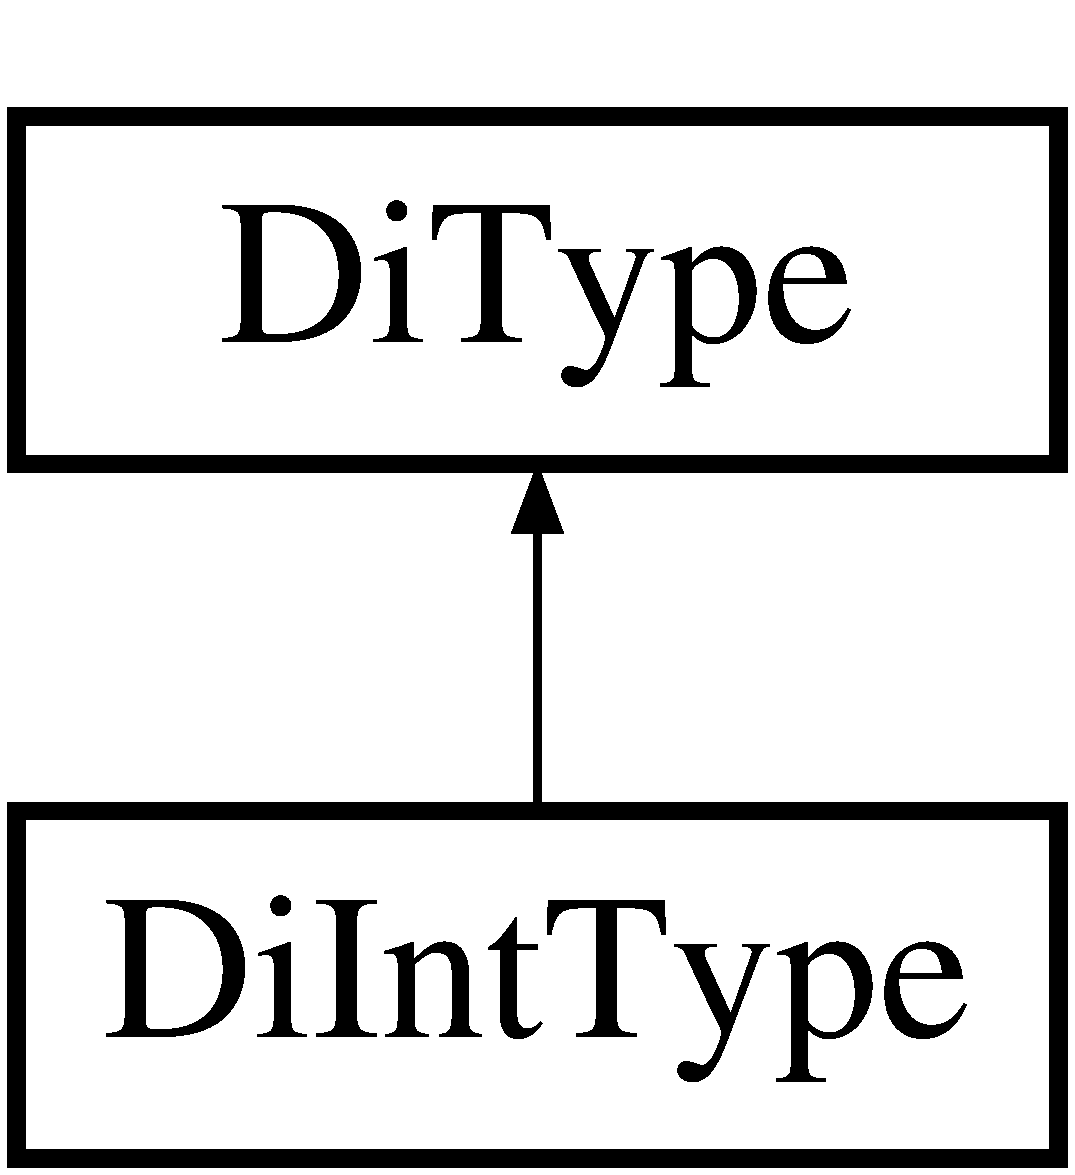
\includegraphics[height=2.000000cm]{class_di_int_type}
\end{center}
\end{figure}
\subsection*{Public Member Functions}
\begin{DoxyCompactItemize}
\item 
\hypertarget{class_di_int_type_aeb0ad81c8fe515c5abbb44a0c6c43c9b}{{\bfseries Di\-Int\-Type} (B\-Patch\-\_\-image \&bp\-Image)}\label{class_di_int_type_aeb0ad81c8fe515c5abbb44a0c6c43c9b}

\end{DoxyCompactItemize}


\subsection{Detailed Description}
Dyninst Int type class. 

\begin{DoxyVersion}{Version}
1.\-0b 
\end{DoxyVersion}
\begin{DoxyAuthor}{Author}
Ania Sikora, 2002 
\end{DoxyAuthor}
\begin{DoxySince}{Since}
1.\-0b 
\end{DoxySince}


The documentation for this class was generated from the following file\-:\begin{DoxyCompactItemize}
\item 
Common/di.\-h\end{DoxyCompactItemize}

\hypertarget{class_di_int_variable}{\section{Di\-Int\-Variable Class Reference}
\label{class_di_int_variable}\index{Di\-Int\-Variable@{Di\-Int\-Variable}}
}


Dyninst's int variable class.  




{\ttfamily \#include $<$di.\-h$>$}

Inheritance diagram for Di\-Int\-Variable\-:\begin{figure}[H]
\begin{center}
\leavevmode
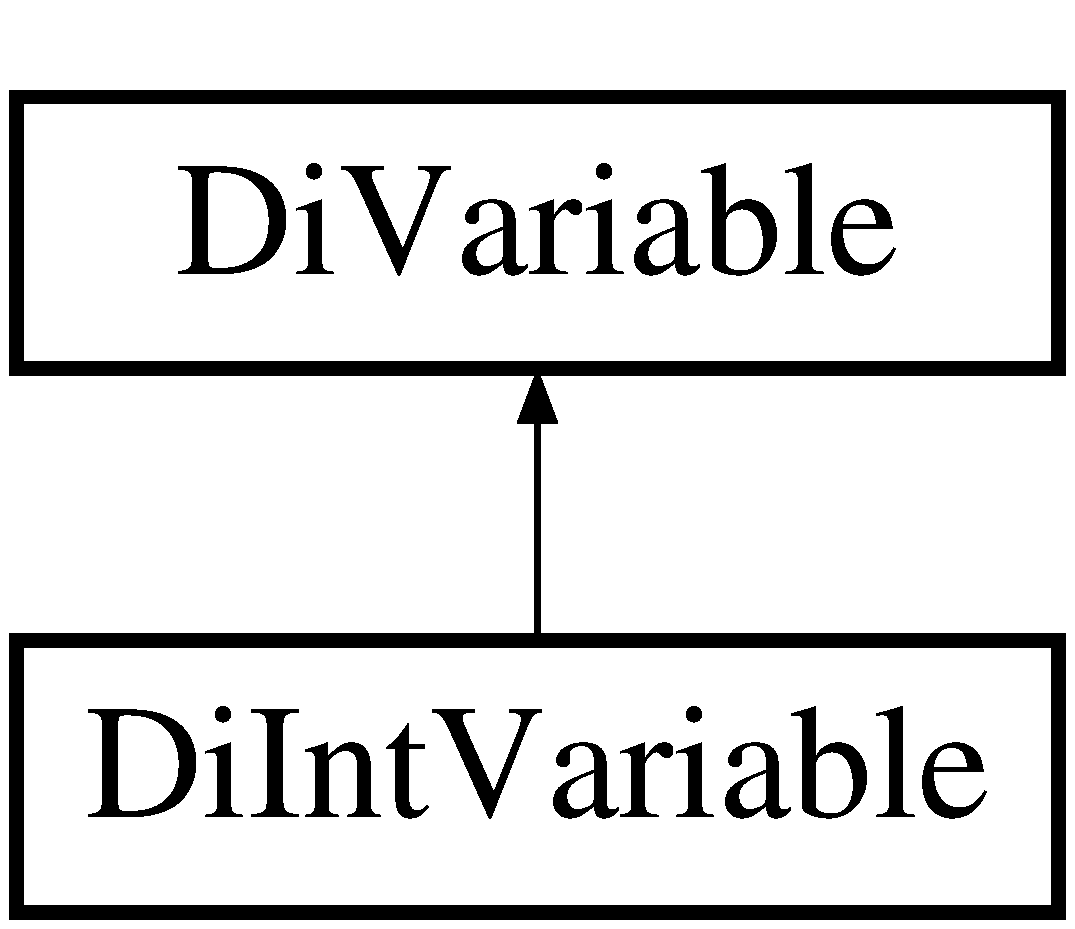
\includegraphics[height=2.000000cm]{class_di_int_variable}
\end{center}
\end{figure}
\subsection*{Public Member Functions}
\begin{DoxyCompactItemize}
\item 
\hypertarget{class_di_int_variable_aa43e23ff3f886dc3ec8266b4d5185d59}{{\bfseries Di\-Int\-Variable} (B\-Patch\-\_\-process \&bp\-Process)}\label{class_di_int_variable_aa43e23ff3f886dc3ec8266b4d5185d59}

\end{DoxyCompactItemize}


\subsection{Detailed Description}
Dyninst's int variable class. 

\begin{DoxyVersion}{Version}
1.\-0b 
\end{DoxyVersion}
\begin{DoxyAuthor}{Author}
Ania Sikora, 2002 
\end{DoxyAuthor}
\begin{DoxySince}{Since}
1.\-0b 
\end{DoxySince}


The documentation for this class was generated from the following file\-:\begin{DoxyCompactItemize}
\item 
Common/di.\-h\end{DoxyCompactItemize}

\hypertarget{class_di_point}{\section{Di\-Point Class Reference}
\label{class_di_point}\index{Di\-Point@{Di\-Point}}
}


Dyninst's point class. An object of this class represents a location in an application's code at which \hyperlink{class_dyn_inst}{Dyn\-Inst} can insert instrumentation.  




{\ttfamily \#include $<$di.\-h$>$}

\subsection*{Public Member Functions}
\begin{DoxyCompactItemize}
\item 
\hyperlink{class_di_point_a0cb0a2a951b711f680f51d7ca6719a83}{Di\-Point} (B\-Patch\-\_\-image \&bp\-Image, string const \&proc\-Name, B\-Patch\-\_\-procedure\-Location loc=B\-Patch\-\_\-entry)
\begin{DoxyCompactList}\small\item\em Finds the given location in the function with a given name. \end{DoxyCompactList}\item 
void \hyperlink{class_di_point_ad4a55eb8bb7e86dacfb443f7d374e3d0}{Get\-Called\-Func\-Name} (char $\ast$buf, int size)
\begin{DoxyCompactList}\small\item\em Getter of the current function name. \end{DoxyCompactList}\item 
unsigned long \hyperlink{class_di_point_ae15f39a73445e20c48d120a43527d354}{Get\-Address} ()
\begin{DoxyCompactList}\small\item\em Getter of the current address. \end{DoxyCompactList}\item 
\hypertarget{class_di_point_a51d22da20645cfd7f51552ac73628032}{{\bfseries operator Point\-Vector \&} ()}\label{class_di_point_a51d22da20645cfd7f51552ac73628032}

\item 
Point\-Vector \& \hyperlink{class_di_point_a592e02eeeb615a57729cb54c9b8cc19b}{get\-Points} ()
\begin{DoxyCompactList}\small\item\em \-\_\-bp\-Points getter \end{DoxyCompactList}\end{DoxyCompactItemize}


\subsection{Detailed Description}
Dyninst's point class. An object of this class represents a location in an application's code at which \hyperlink{class_dyn_inst}{Dyn\-Inst} can insert instrumentation. 

\begin{DoxyVersion}{Version}
1.\-0b 
\end{DoxyVersion}
\begin{DoxyAuthor}{Author}
Ania Sikora, 2002 
\end{DoxyAuthor}
\begin{DoxySince}{Since}
1.\-0b 
\end{DoxySince}


\subsection{Constructor \& Destructor Documentation}
\hypertarget{class_di_point_a0cb0a2a951b711f680f51d7ca6719a83}{\index{Di\-Point@{Di\-Point}!Di\-Point@{Di\-Point}}
\index{Di\-Point@{Di\-Point}!DiPoint@{Di\-Point}}
\subsubsection[{Di\-Point}]{\setlength{\rightskip}{0pt plus 5cm}Di\-Point\-::\-Di\-Point (
\begin{DoxyParamCaption}
\item[{B\-Patch\-\_\-image \&}]{bp\-Image, }
\item[{string const \&}]{proc\-Name, }
\item[{B\-Patch\-\_\-procedure\-Location}]{loc = {\ttfamily BPatch\-\_\-entry}}
\end{DoxyParamCaption}
)}}\label{class_di_point_a0cb0a2a951b711f680f51d7ca6719a83}


Finds the given location in the function with a given name. 


\begin{DoxyParams}{Parameters}
{\em bp\-Image} & B\-Patch Image of the program \\
\hline
{\em proc\-Name} & Process Name \\
\hline
{\em loc} & Location \\
\hline
\end{DoxyParams}


\subsection{Member Function Documentation}
\hypertarget{class_di_point_ae15f39a73445e20c48d120a43527d354}{\index{Di\-Point@{Di\-Point}!Get\-Address@{Get\-Address}}
\index{Get\-Address@{Get\-Address}!DiPoint@{Di\-Point}}
\subsubsection[{Get\-Address}]{\setlength{\rightskip}{0pt plus 5cm}unsigned long Di\-Point\-::\-Get\-Address (
\begin{DoxyParamCaption}
{}
\end{DoxyParamCaption}
)}}\label{class_di_point_ae15f39a73445e20c48d120a43527d354}


Getter of the current address. 

\begin{DoxyReturn}{Returns}
address 
\end{DoxyReturn}
\hypertarget{class_di_point_ad4a55eb8bb7e86dacfb443f7d374e3d0}{\index{Di\-Point@{Di\-Point}!Get\-Called\-Func\-Name@{Get\-Called\-Func\-Name}}
\index{Get\-Called\-Func\-Name@{Get\-Called\-Func\-Name}!DiPoint@{Di\-Point}}
\subsubsection[{Get\-Called\-Func\-Name}]{\setlength{\rightskip}{0pt plus 5cm}void Di\-Point\-::\-Get\-Called\-Func\-Name (
\begin{DoxyParamCaption}
\item[{char $\ast$}]{buf, }
\item[{int}]{size}
\end{DoxyParamCaption}
)}}\label{class_di_point_ad4a55eb8bb7e86dacfb443f7d374e3d0}


Getter of the current function name. 


\begin{DoxyParams}{Parameters}
{\em buf} & Returned name \\
\hline
{\em size} & Max length of the buffer \\
\hline
\end{DoxyParams}
\hypertarget{class_di_point_a592e02eeeb615a57729cb54c9b8cc19b}{\index{Di\-Point@{Di\-Point}!get\-Points@{get\-Points}}
\index{get\-Points@{get\-Points}!DiPoint@{Di\-Point}}
\subsubsection[{get\-Points}]{\setlength{\rightskip}{0pt plus 5cm}Point\-Vector\& Di\-Point\-::get\-Points (
\begin{DoxyParamCaption}
{}
\end{DoxyParamCaption}
)\hspace{0.3cm}{\ttfamily [inline]}}}\label{class_di_point_a592e02eeeb615a57729cb54c9b8cc19b}


\-\_\-bp\-Points getter 

\begin{DoxyReturn}{Returns}
\-\_\-bp\-Points 
\end{DoxyReturn}


The documentation for this class was generated from the following files\-:\begin{DoxyCompactItemize}
\item 
Common/di.\-h\item 
Common/di.\-cpp\end{DoxyCompactItemize}

\hypertarget{class_di_process}{\section{Di\-Process Class Reference}
\label{class_di_process}\index{Di\-Process@{Di\-Process}}
}


Operates on code in execution. This class can be used to manipulate the process.  




{\ttfamily \#include $<$di.\-h$>$}

\subsection*{Public Member Functions}
\begin{DoxyCompactItemize}
\item 
\hyperlink{class_di_process_abc88219761bfa55e5b3b0ce31fd0721c}{Di\-Process} ()
\item 
\hyperlink{class_di_process_a29fffcfa25576de71c6b0dd64b1b166a}{Di\-Process} (char $\ast$mutatee\-Name, int pid)
\begin{DoxyCompactList}\small\item\em Attaches the program to a running process. \end{DoxyCompactList}\item 
\hyperlink{class_di_process_abe9d867d2622eddf74ab7cdc2951bd7b}{Di\-Process} (char $\ast$mutatee\-Name, char $\ast$argv\mbox{[}$\,$\mbox{]}, char $\ast$envp\mbox{[}$\,$\mbox{]}=0)
\begin{DoxyCompactList}\small\item\em Creates the program with the given arguments. \end{DoxyCompactList}\item 
\hyperlink{class_di_process_af93de25bc325bea42a69c2df0fee7075}{Di\-Process} (char $\ast$mutatee\-Name)
\begin{DoxyCompactList}\small\item\em Creates the program (mutatee) \end{DoxyCompactList}\item 
\hypertarget{class_di_process_a7c46390461846d2baaff0164e5122ab7}{\hyperlink{class_di_process_a7c46390461846d2baaff0164e5122ab7}{$\sim$\-Di\-Process} ()}\label{class_di_process_a7c46390461846d2baaff0164e5122ab7}

\begin{DoxyCompactList}\small\item\em Destructor. \end{DoxyCompactList}\item 
\hypertarget{class_di_process_a1c1615ae17ce6fa1d9a0b129db349e2b}{{\bfseries operator B\-Patch\-\_\-process \&} ()}\label{class_di_process_a1c1615ae17ce6fa1d9a0b129db349e2b}

\item 
int \hyperlink{class_di_process_ad83360d6f92a6ef991ad44075964fa85}{Get\-Pid} ()
\begin{DoxyCompactList}\small\item\em Getter of the Pid. \end{DoxyCompactList}\item 
bool \hyperlink{class_di_process_a2e92f5f654ba4d0bc9f495cd58c571b2}{Is\-Stopped} ()
\begin{DoxyCompactList}\small\item\em Asserts that \-\_\-bp\-Process has been created and returns a boolean. \end{DoxyCompactList}\item 
B\-Patch\-Snippet\-Handle $\ast$ \hyperlink{class_di_process_a3dc12883c432036edb7ea980ccdfa7d3}{Insert\-Snippet} (B\-Patch\-\_\-snippet const \&expr, B\-Patch\-\_\-point \&point)
\begin{DoxyCompactList}\small\item\em Inserts a given snippet into the given point. \end{DoxyCompactList}\item 
B\-Patch\-Snippet\-Handle $\ast$ \hyperlink{class_di_process_a3d0cdbd8bae78306b311b03403e7fa8d}{Insert\-Snippet} (B\-Patch\-\_\-snippet const \&expr, B\-Patch\-\_\-point \&point, B\-Patch\-\_\-call\-When when, B\-Patch\-\_\-snippet\-Order order)
\begin{DoxyCompactList}\small\item\em Inserts the snippet into the point in a given order. \end{DoxyCompactList}\item 
B\-Patch\-Snippet\-Handle $\ast$ \hyperlink{class_di_process_aec944980cc04cb6e05f2b033971d819e}{Insert\-Snippet\-Before} (B\-Patch\-\_\-snippet const \&expr, B\-Patch\-\_\-point \&point)
\begin{DoxyCompactList}\small\item\em Inserts a given snippet before the given point. \end{DoxyCompactList}\item 
B\-Patch\-Snippet\-Handle $\ast$ \hyperlink{class_di_process_af381488cf52e8a790b0476c1d4da9c4f}{Insert\-Snippet\-After} (B\-Patch\-\_\-snippet const \&expr, B\-Patch\-\_\-point \&point)
\begin{DoxyCompactList}\small\item\em Inserts a given snippet after the given point. \end{DoxyCompactList}\item 
B\-Patch\-Snippet\-Handle $\ast$ \hyperlink{class_di_process_a79ae7629dedcd84ab0776deaa166f7c4}{Insert\-Snippet} (B\-Patch\-\_\-snippet const \&expr, Point\-Vector \&points)
\begin{DoxyCompactList}\small\item\em Inserts the given snippet in the given points. \end{DoxyCompactList}\item 
B\-Patch\-Snippet\-Handle $\ast$ \hyperlink{class_di_process_a39c00229b7533befd6edb616ce9df787}{Insert\-Snippet} (B\-Patch\-\_\-snippet const \&expr, Point\-Vector \&points, B\-Patch\-\_\-call\-When when, B\-Patch\-\_\-snippet\-Order order)
\begin{DoxyCompactList}\small\item\em Inserts the given snippet in the series of points with the given order and moment. \end{DoxyCompactList}\item 
B\-Patch\-Snippet\-Handle $\ast$ \hyperlink{class_di_process_af6bcde05d9750fbba96e94da27116ac7}{Insert\-Snippet\-Before} (B\-Patch\-\_\-snippet const \&expr, Point\-Vector \&points)
\begin{DoxyCompactList}\small\item\em Inserts the snippet before the given points. \end{DoxyCompactList}\item 
B\-Patch\-Snippet\-Handle $\ast$ \hyperlink{class_di_process_a4efe5b0907efbcd8b95d681336e58a65}{Insert\-Snippet\-After} (B\-Patch\-\_\-snippet const \&expr, Point\-Vector \&points)
\begin{DoxyCompactList}\small\item\em Inserts the snippet after the given points. \end{DoxyCompactList}\item 
void \hyperlink{class_di_process_a1358a94954ae1ef6d3fbffafbd95b567}{Delete\-Snippet} (B\-Patch\-Snippet\-Handle $\ast$handle)
\begin{DoxyCompactList}\small\item\em Deletes the snippet in the given handle. \end{DoxyCompactList}\item 
void \hyperlink{class_di_process_aa83c0791594eddab08a1a0e5952c5e5a}{One\-Time\-Code} (B\-Patch\-\_\-snippet const \&expr)
\begin{DoxyCompactList}\small\item\em Executes the given snippet once. \end{DoxyCompactList}\item 
void \hyperlink{class_di_process_a73bd02c4104451077f2622efd1c708d6}{Replace\-Function} (B\-Patch\-\_\-function \&old\-Func, B\-Patch\-\_\-function \&new\-Func)
\begin{DoxyCompactList}\small\item\em Replaces a function call with a call to another function. \end{DoxyCompactList}\item 
\hypertarget{class_di_process_a047096a8e3be003544529f1ddfa4d3c5}{void \hyperlink{class_di_process_a047096a8e3be003544529f1ddfa4d3c5}{Continue\-Execution} ()}\label{class_di_process_a047096a8e3be003544529f1ddfa4d3c5}

\begin{DoxyCompactList}\small\item\em Resumes the execution of mutatee process. \end{DoxyCompactList}\item 
bool \hyperlink{class_di_process_afa4a0216ebd254a2d353b79ac1c197fe}{Stop\-Execution} ()
\begin{DoxyCompactList}\small\item\em Stops the execution of the mutatee process. \end{DoxyCompactList}\item 
\hypertarget{class_di_process_a9acf14711e3036fe76342fd9405ea933}{void \hyperlink{class_di_process_a9acf14711e3036fe76342fd9405ea933}{Wait\-For} ()}\label{class_di_process_a9acf14711e3036fe76342fd9405ea933}

\begin{DoxyCompactList}\small\item\em Waits for the termination of the process. \end{DoxyCompactList}\item 
\hypertarget{class_di_process_a3a0f5ac09a216b99bd43b8ad85d3ec46}{void \hyperlink{class_di_process_a3a0f5ac09a216b99bd43b8ad85d3ec46}{Test} ()}\label{class_di_process_a3a0f5ac09a216b99bd43b8ad85d3ec46}

\begin{DoxyCompactList}\small\item\em Tests the current mutatee process by waiting for a status change. \end{DoxyCompactList}\item 
bool \hyperlink{class_di_process_ad70fc9c4feb2c10e1810ea7b988cb87f}{Terminate} ()
\begin{DoxyCompactList}\small\item\em Terminates the mutatee process. \end{DoxyCompactList}\item 
bool \hyperlink{class_di_process_a9dece6fa09fa876026e6f0d989dd2b31}{Is\-Terminated} ()
\begin{DoxyCompactList}\small\item\em Returns true if the mutatee process is terminated. \end{DoxyCompactList}\item 
\hypertarget{class_di_process_a55905bd1802af67249338f65deec5b9d}{void \hyperlink{class_di_process_a55905bd1802af67249338f65deec5b9d}{Wait\-For\-Stop} ()}\label{class_di_process_a55905bd1802af67249338f65deec5b9d}

\begin{DoxyCompactList}\small\item\em Waits for the mutatee process to stop. \end{DoxyCompactList}\item 
void \hyperlink{class_di_process_a49c36844b4f223edb54b23e5bc3530d0}{load\-Library} (char $\ast$lib\-Name)
\begin{DoxyCompactList}\small\item\em Loads a shared library into the mutatee's address space. Returns true if successful. \end{DoxyCompactList}\item 
void \hyperlink{class_di_process_a3fabae8f482f0141effb044bd5550850}{Get\-Line\-Number} (unsigned long addr, unsigned short \&line, char $\ast$file\-Name, int length)
\begin{DoxyCompactList}\small\item\em Gets information about the given line number from the mutatee process. \end{DoxyCompactList}\item 
B\-Patch\-\_\-variable\-Expr $\ast$ \hyperlink{class_di_process_af5dbaaf631e3a3746bfa5878a46999e8}{Malloc} (B\-Patch\-\_\-type \&type)
\begin{DoxyCompactList}\small\item\em Allocates a new variable of the given type. \end{DoxyCompactList}\end{DoxyCompactItemize}


\subsection{Detailed Description}
Operates on code in execution. This class can be used to manipulate the process. 

\begin{DoxyVersion}{Version}
1.\-0b 
\end{DoxyVersion}
\begin{DoxyAuthor}{Author}
Ania Sikora, 2002 
\end{DoxyAuthor}
\begin{DoxySince}{Since}
1.\-0b 
\end{DoxySince}


\subsection{Constructor \& Destructor Documentation}
\hypertarget{class_di_process_abc88219761bfa55e5b3b0ce31fd0721c}{\index{Di\-Process@{Di\-Process}!Di\-Process@{Di\-Process}}
\index{Di\-Process@{Di\-Process}!DiProcess@{Di\-Process}}
\subsubsection[{Di\-Process}]{\setlength{\rightskip}{0pt plus 5cm}Di\-Process\-::\-Di\-Process (
\begin{DoxyParamCaption}
{}
\end{DoxyParamCaption}
)\hspace{0.3cm}{\ttfamily [inline]}}}\label{class_di_process_abc88219761bfa55e5b3b0ce31fd0721c}
\begin{DoxyRefDesc}{Deprecated}
\item[\hyperlink{deprecated__deprecated000002}{Deprecated}]\end{DoxyRefDesc}
\hypertarget{class_di_process_a29fffcfa25576de71c6b0dd64b1b166a}{\index{Di\-Process@{Di\-Process}!Di\-Process@{Di\-Process}}
\index{Di\-Process@{Di\-Process}!DiProcess@{Di\-Process}}
\subsubsection[{Di\-Process}]{\setlength{\rightskip}{0pt plus 5cm}Di\-Process\-::\-Di\-Process (
\begin{DoxyParamCaption}
\item[{char $\ast$}]{mutatee\-Name, }
\item[{int}]{pid}
\end{DoxyParamCaption}
)}}\label{class_di_process_a29fffcfa25576de71c6b0dd64b1b166a}


Attaches the program to a running process. 


\begin{DoxyParams}{Parameters}
{\em mutatee\-Name} & Name of the mutatee \\
\hline
{\em pid} & P\-I\-D to give to the process \\
\hline
\end{DoxyParams}
\hypertarget{class_di_process_abe9d867d2622eddf74ab7cdc2951bd7b}{\index{Di\-Process@{Di\-Process}!Di\-Process@{Di\-Process}}
\index{Di\-Process@{Di\-Process}!DiProcess@{Di\-Process}}
\subsubsection[{Di\-Process}]{\setlength{\rightskip}{0pt plus 5cm}Di\-Process\-::\-Di\-Process (
\begin{DoxyParamCaption}
\item[{char $\ast$}]{mutatee\-Name, }
\item[{char $\ast$}]{argv\mbox{[}$\,$\mbox{]}, }
\item[{char $\ast$}]{envp\mbox{[}$\,$\mbox{]} = {\ttfamily 0}}
\end{DoxyParamCaption}
)}}\label{class_di_process_abe9d867d2622eddf74ab7cdc2951bd7b}


Creates the program with the given arguments. 


\begin{DoxyParams}{Parameters}
{\em mutatee\-Name} & Name of the mutatee \\
\hline
{\em argv} & Arguments to give to the program. This cannot be null \\
\hline
{\em envp} & Environment list \\
\hline
\end{DoxyParams}
\hypertarget{class_di_process_af93de25bc325bea42a69c2df0fee7075}{\index{Di\-Process@{Di\-Process}!Di\-Process@{Di\-Process}}
\index{Di\-Process@{Di\-Process}!DiProcess@{Di\-Process}}
\subsubsection[{Di\-Process}]{\setlength{\rightskip}{0pt plus 5cm}Di\-Process\-::\-Di\-Process (
\begin{DoxyParamCaption}
\item[{char $\ast$}]{mutatee\-Name}
\end{DoxyParamCaption}
)}}\label{class_di_process_af93de25bc325bea42a69c2df0fee7075}


Creates the program (mutatee) 


\begin{DoxyParams}{Parameters}
{\em mutatee\-Name} & Name of the mutatee \\
\hline
\end{DoxyParams}


\subsection{Member Function Documentation}
\hypertarget{class_di_process_a1358a94954ae1ef6d3fbffafbd95b567}{\index{Di\-Process@{Di\-Process}!Delete\-Snippet@{Delete\-Snippet}}
\index{Delete\-Snippet@{Delete\-Snippet}!DiProcess@{Di\-Process}}
\subsubsection[{Delete\-Snippet}]{\setlength{\rightskip}{0pt plus 5cm}void Di\-Process\-::\-Delete\-Snippet (
\begin{DoxyParamCaption}
\item[{B\-Patch\-Snippet\-Handle $\ast$}]{handle}
\end{DoxyParamCaption}
)}}\label{class_di_process_a1358a94954ae1ef6d3fbffafbd95b567}


Deletes the snippet in the given handle. 


\begin{DoxyParams}{Parameters}
{\em handle} & \\
\hline
\end{DoxyParams}
\hypertarget{class_di_process_a3fabae8f482f0141effb044bd5550850}{\index{Di\-Process@{Di\-Process}!Get\-Line\-Number@{Get\-Line\-Number}}
\index{Get\-Line\-Number@{Get\-Line\-Number}!DiProcess@{Di\-Process}}
\subsubsection[{Get\-Line\-Number}]{\setlength{\rightskip}{0pt plus 5cm}void Di\-Process\-::\-Get\-Line\-Number (
\begin{DoxyParamCaption}
\item[{unsigned long}]{addr, }
\item[{unsigned short \&}]{line, }
\item[{char $\ast$}]{file\-Name, }
\item[{int}]{length}
\end{DoxyParamCaption}
)}}\label{class_di_process_a3fabae8f482f0141effb044bd5550850}


Gets information about the given line number from the mutatee process. 


\begin{DoxyParams}{Parameters}
{\em addr} & \\
\hline
{\em line} & \\
\hline
{\em file\-Name} & \\
\hline
{\em length} & \\
\hline
\end{DoxyParams}
\hypertarget{class_di_process_ad83360d6f92a6ef991ad44075964fa85}{\index{Di\-Process@{Di\-Process}!Get\-Pid@{Get\-Pid}}
\index{Get\-Pid@{Get\-Pid}!DiProcess@{Di\-Process}}
\subsubsection[{Get\-Pid}]{\setlength{\rightskip}{0pt plus 5cm}int Di\-Process\-::\-Get\-Pid (
\begin{DoxyParamCaption}
{}
\end{DoxyParamCaption}
)\hspace{0.3cm}{\ttfamily [inline]}}}\label{class_di_process_ad83360d6f92a6ef991ad44075964fa85}


Getter of the Pid. 

\begin{DoxyReturn}{Returns}
Pid 
\end{DoxyReturn}
\hypertarget{class_di_process_a3dc12883c432036edb7ea980ccdfa7d3}{\index{Di\-Process@{Di\-Process}!Insert\-Snippet@{Insert\-Snippet}}
\index{Insert\-Snippet@{Insert\-Snippet}!DiProcess@{Di\-Process}}
\subsubsection[{Insert\-Snippet}]{\setlength{\rightskip}{0pt plus 5cm}B\-Patch\-Snippet\-Handle $\ast$ Di\-Process\-::\-Insert\-Snippet (
\begin{DoxyParamCaption}
\item[{B\-Patch\-\_\-snippet const \&}]{expr, }
\item[{B\-Patch\-\_\-point \&}]{point}
\end{DoxyParamCaption}
)}}\label{class_di_process_a3dc12883c432036edb7ea980ccdfa7d3}


Inserts a given snippet into the given point. 


\begin{DoxyParams}{Parameters}
{\em expr} & Snippet \\
\hline
{\em point} & Point where the Snippet will be inserted\\
\hline
\end{DoxyParams}
\begin{DoxyReturn}{Returns}
Handle 
\end{DoxyReturn}
\hypertarget{class_di_process_a3d0cdbd8bae78306b311b03403e7fa8d}{\index{Di\-Process@{Di\-Process}!Insert\-Snippet@{Insert\-Snippet}}
\index{Insert\-Snippet@{Insert\-Snippet}!DiProcess@{Di\-Process}}
\subsubsection[{Insert\-Snippet}]{\setlength{\rightskip}{0pt plus 5cm}B\-Patch\-Snippet\-Handle $\ast$ Di\-Process\-::\-Insert\-Snippet (
\begin{DoxyParamCaption}
\item[{B\-Patch\-\_\-snippet const \&}]{expr, }
\item[{B\-Patch\-\_\-point \&}]{point, }
\item[{B\-Patch\-\_\-call\-When}]{when, }
\item[{B\-Patch\-\_\-snippet\-Order}]{order}
\end{DoxyParamCaption}
)}}\label{class_di_process_a3d0cdbd8bae78306b311b03403e7fa8d}


Inserts the snippet into the point in a given order. 


\begin{DoxyParams}{Parameters}
{\em expr} & Snippet \\
\hline
{\em point} & Point where the Snippet will be inserted \\
\hline
{\em when} & \\
\hline
{\em order} & \\
\hline
\end{DoxyParams}
\begin{DoxyReturn}{Returns}
Handle 
\end{DoxyReturn}
\hypertarget{class_di_process_a79ae7629dedcd84ab0776deaa166f7c4}{\index{Di\-Process@{Di\-Process}!Insert\-Snippet@{Insert\-Snippet}}
\index{Insert\-Snippet@{Insert\-Snippet}!DiProcess@{Di\-Process}}
\subsubsection[{Insert\-Snippet}]{\setlength{\rightskip}{0pt plus 5cm}B\-Patch\-Snippet\-Handle $\ast$ Di\-Process\-::\-Insert\-Snippet (
\begin{DoxyParamCaption}
\item[{B\-Patch\-\_\-snippet const \&}]{expr, }
\item[{Point\-Vector \&}]{points}
\end{DoxyParamCaption}
)}}\label{class_di_process_a79ae7629dedcd84ab0776deaa166f7c4}


Inserts the given snippet in the given points. 


\begin{DoxyParams}{Parameters}
{\em expr} & Snippet \\
\hline
{\em points} & Vector of points\\
\hline
\end{DoxyParams}
\begin{DoxyReturn}{Returns}
Handle 
\end{DoxyReturn}
\hypertarget{class_di_process_a39c00229b7533befd6edb616ce9df787}{\index{Di\-Process@{Di\-Process}!Insert\-Snippet@{Insert\-Snippet}}
\index{Insert\-Snippet@{Insert\-Snippet}!DiProcess@{Di\-Process}}
\subsubsection[{Insert\-Snippet}]{\setlength{\rightskip}{0pt plus 5cm}B\-Patch\-Snippet\-Handle $\ast$ Di\-Process\-::\-Insert\-Snippet (
\begin{DoxyParamCaption}
\item[{B\-Patch\-\_\-snippet const \&}]{expr, }
\item[{Point\-Vector \&}]{points, }
\item[{B\-Patch\-\_\-call\-When}]{when, }
\item[{B\-Patch\-\_\-snippet\-Order}]{order}
\end{DoxyParamCaption}
)}}\label{class_di_process_a39c00229b7533befd6edb616ce9df787}


Inserts the given snippet in the series of points with the given order and moment. 


\begin{DoxyParams}{Parameters}
{\em expr} & Snippet \\
\hline
{\em points} & Vector of points \\
\hline
{\em when} & \\
\hline
{\em order} & \\
\hline
\end{DoxyParams}
\begin{DoxyReturn}{Returns}
Handle 
\end{DoxyReturn}
\hypertarget{class_di_process_af381488cf52e8a790b0476c1d4da9c4f}{\index{Di\-Process@{Di\-Process}!Insert\-Snippet\-After@{Insert\-Snippet\-After}}
\index{Insert\-Snippet\-After@{Insert\-Snippet\-After}!DiProcess@{Di\-Process}}
\subsubsection[{Insert\-Snippet\-After}]{\setlength{\rightskip}{0pt plus 5cm}B\-Patch\-Snippet\-Handle $\ast$ Di\-Process\-::\-Insert\-Snippet\-After (
\begin{DoxyParamCaption}
\item[{B\-Patch\-\_\-snippet const \&}]{expr, }
\item[{B\-Patch\-\_\-point \&}]{point}
\end{DoxyParamCaption}
)}}\label{class_di_process_af381488cf52e8a790b0476c1d4da9c4f}


Inserts a given snippet after the given point. 


\begin{DoxyParams}{Parameters}
{\em expr} & Snippet \\
\hline
{\em point} & Point where the Snippet will be inserted\\
\hline
\end{DoxyParams}
\begin{DoxyReturn}{Returns}
Handle 
\end{DoxyReturn}
\hypertarget{class_di_process_a4efe5b0907efbcd8b95d681336e58a65}{\index{Di\-Process@{Di\-Process}!Insert\-Snippet\-After@{Insert\-Snippet\-After}}
\index{Insert\-Snippet\-After@{Insert\-Snippet\-After}!DiProcess@{Di\-Process}}
\subsubsection[{Insert\-Snippet\-After}]{\setlength{\rightskip}{0pt plus 5cm}B\-Patch\-Snippet\-Handle $\ast$ Di\-Process\-::\-Insert\-Snippet\-After (
\begin{DoxyParamCaption}
\item[{B\-Patch\-\_\-snippet const \&}]{expr, }
\item[{Point\-Vector \&}]{points}
\end{DoxyParamCaption}
)}}\label{class_di_process_a4efe5b0907efbcd8b95d681336e58a65}


Inserts the snippet after the given points. 


\begin{DoxyParams}{Parameters}
{\em expr} & Snippet \\
\hline
{\em points} & Vector of points\\
\hline
\end{DoxyParams}
\begin{DoxyReturn}{Returns}
Handle 
\end{DoxyReturn}
\hypertarget{class_di_process_aec944980cc04cb6e05f2b033971d819e}{\index{Di\-Process@{Di\-Process}!Insert\-Snippet\-Before@{Insert\-Snippet\-Before}}
\index{Insert\-Snippet\-Before@{Insert\-Snippet\-Before}!DiProcess@{Di\-Process}}
\subsubsection[{Insert\-Snippet\-Before}]{\setlength{\rightskip}{0pt plus 5cm}B\-Patch\-Snippet\-Handle $\ast$ Di\-Process\-::\-Insert\-Snippet\-Before (
\begin{DoxyParamCaption}
\item[{B\-Patch\-\_\-snippet const \&}]{expr, }
\item[{B\-Patch\-\_\-point \&}]{point}
\end{DoxyParamCaption}
)}}\label{class_di_process_aec944980cc04cb6e05f2b033971d819e}


Inserts a given snippet before the given point. 


\begin{DoxyParams}{Parameters}
{\em expr} & Snippet \\
\hline
{\em point} & Point where the Snippet will be inserted\\
\hline
\end{DoxyParams}
\begin{DoxyReturn}{Returns}
Handle 
\end{DoxyReturn}
\hypertarget{class_di_process_af6bcde05d9750fbba96e94da27116ac7}{\index{Di\-Process@{Di\-Process}!Insert\-Snippet\-Before@{Insert\-Snippet\-Before}}
\index{Insert\-Snippet\-Before@{Insert\-Snippet\-Before}!DiProcess@{Di\-Process}}
\subsubsection[{Insert\-Snippet\-Before}]{\setlength{\rightskip}{0pt plus 5cm}B\-Patch\-Snippet\-Handle $\ast$ Di\-Process\-::\-Insert\-Snippet\-Before (
\begin{DoxyParamCaption}
\item[{B\-Patch\-\_\-snippet const \&}]{expr, }
\item[{Point\-Vector \&}]{points}
\end{DoxyParamCaption}
)}}\label{class_di_process_af6bcde05d9750fbba96e94da27116ac7}


Inserts the snippet before the given points. 


\begin{DoxyParams}{Parameters}
{\em expr} & Snippet \\
\hline
{\em points} & Vector of points\\
\hline
\end{DoxyParams}
\begin{DoxyReturn}{Returns}
Handle 
\end{DoxyReturn}
\hypertarget{class_di_process_a2e92f5f654ba4d0bc9f495cd58c571b2}{\index{Di\-Process@{Di\-Process}!Is\-Stopped@{Is\-Stopped}}
\index{Is\-Stopped@{Is\-Stopped}!DiProcess@{Di\-Process}}
\subsubsection[{Is\-Stopped}]{\setlength{\rightskip}{0pt plus 5cm}bool Di\-Process\-::\-Is\-Stopped (
\begin{DoxyParamCaption}
{}
\end{DoxyParamCaption}
)\hspace{0.3cm}{\ttfamily [inline]}}}\label{class_di_process_a2e92f5f654ba4d0bc9f495cd58c571b2}


Asserts that \-\_\-bp\-Process has been created and returns a boolean. 

\begin{DoxyReturn}{Returns}
bool 
\end{DoxyReturn}
\hypertarget{class_di_process_a9dece6fa09fa876026e6f0d989dd2b31}{\index{Di\-Process@{Di\-Process}!Is\-Terminated@{Is\-Terminated}}
\index{Is\-Terminated@{Is\-Terminated}!DiProcess@{Di\-Process}}
\subsubsection[{Is\-Terminated}]{\setlength{\rightskip}{0pt plus 5cm}bool Di\-Process\-::\-Is\-Terminated (
\begin{DoxyParamCaption}
{}
\end{DoxyParamCaption}
)\hspace{0.3cm}{\ttfamily [inline]}}}\label{class_di_process_a9dece6fa09fa876026e6f0d989dd2b31}


Returns true if the mutatee process is terminated. 

\begin{DoxyReturn}{Returns}
bool 
\end{DoxyReturn}
\hypertarget{class_di_process_a49c36844b4f223edb54b23e5bc3530d0}{\index{Di\-Process@{Di\-Process}!load\-Library@{load\-Library}}
\index{load\-Library@{load\-Library}!DiProcess@{Di\-Process}}
\subsubsection[{load\-Library}]{\setlength{\rightskip}{0pt plus 5cm}void Di\-Process\-::load\-Library (
\begin{DoxyParamCaption}
\item[{char $\ast$}]{lib\-Name}
\end{DoxyParamCaption}
)}}\label{class_di_process_a49c36844b4f223edb54b23e5bc3530d0}


Loads a shared library into the mutatee's address space. Returns true if successful. 


\begin{DoxyParams}{Parameters}
{\em lib\-Name} & Library name \\
\hline
\end{DoxyParams}
\hypertarget{class_di_process_af5dbaaf631e3a3746bfa5878a46999e8}{\index{Di\-Process@{Di\-Process}!Malloc@{Malloc}}
\index{Malloc@{Malloc}!DiProcess@{Di\-Process}}
\subsubsection[{Malloc}]{\setlength{\rightskip}{0pt plus 5cm}B\-Patch\-\_\-variable\-Expr$\ast$ Di\-Process\-::\-Malloc (
\begin{DoxyParamCaption}
\item[{B\-Patch\-\_\-type \&}]{type}
\end{DoxyParamCaption}
)\hspace{0.3cm}{\ttfamily [inline]}}}\label{class_di_process_af5dbaaf631e3a3746bfa5878a46999e8}


Allocates a new variable of the given type. 


\begin{DoxyParams}{Parameters}
{\em type} & \\
\hline
\end{DoxyParams}
\hypertarget{class_di_process_aa83c0791594eddab08a1a0e5952c5e5a}{\index{Di\-Process@{Di\-Process}!One\-Time\-Code@{One\-Time\-Code}}
\index{One\-Time\-Code@{One\-Time\-Code}!DiProcess@{Di\-Process}}
\subsubsection[{One\-Time\-Code}]{\setlength{\rightskip}{0pt plus 5cm}void Di\-Process\-::\-One\-Time\-Code (
\begin{DoxyParamCaption}
\item[{B\-Patch\-\_\-snippet const \&}]{expr}
\end{DoxyParamCaption}
)}}\label{class_di_process_aa83c0791594eddab08a1a0e5952c5e5a}


Executes the given snippet once. 


\begin{DoxyParams}{Parameters}
{\em expr} & Snippet \\
\hline
\end{DoxyParams}
\hypertarget{class_di_process_a73bd02c4104451077f2622efd1c708d6}{\index{Di\-Process@{Di\-Process}!Replace\-Function@{Replace\-Function}}
\index{Replace\-Function@{Replace\-Function}!DiProcess@{Di\-Process}}
\subsubsection[{Replace\-Function}]{\setlength{\rightskip}{0pt plus 5cm}void Di\-Process\-::\-Replace\-Function (
\begin{DoxyParamCaption}
\item[{B\-Patch\-\_\-function \&}]{old\-Func, }
\item[{B\-Patch\-\_\-function \&}]{new\-Func}
\end{DoxyParamCaption}
)}}\label{class_di_process_a73bd02c4104451077f2622efd1c708d6}


Replaces a function call with a call to another function. 


\begin{DoxyParams}{Parameters}
{\em old\-Func} & \\
\hline
{\em new\-Func} & \\
\hline
\end{DoxyParams}
\hypertarget{class_di_process_afa4a0216ebd254a2d353b79ac1c197fe}{\index{Di\-Process@{Di\-Process}!Stop\-Execution@{Stop\-Execution}}
\index{Stop\-Execution@{Stop\-Execution}!DiProcess@{Di\-Process}}
\subsubsection[{Stop\-Execution}]{\setlength{\rightskip}{0pt plus 5cm}bool Di\-Process\-::\-Stop\-Execution (
\begin{DoxyParamCaption}
{}
\end{DoxyParamCaption}
)\hspace{0.3cm}{\ttfamily [inline]}}}\label{class_di_process_afa4a0216ebd254a2d353b79ac1c197fe}


Stops the execution of the mutatee process. 

\begin{DoxyReturn}{Returns}
bool 
\end{DoxyReturn}
\hypertarget{class_di_process_ad70fc9c4feb2c10e1810ea7b988cb87f}{\index{Di\-Process@{Di\-Process}!Terminate@{Terminate}}
\index{Terminate@{Terminate}!DiProcess@{Di\-Process}}
\subsubsection[{Terminate}]{\setlength{\rightskip}{0pt plus 5cm}bool Di\-Process\-::\-Terminate (
\begin{DoxyParamCaption}
{}
\end{DoxyParamCaption}
)\hspace{0.3cm}{\ttfamily [inline]}}}\label{class_di_process_ad70fc9c4feb2c10e1810ea7b988cb87f}


Terminates the mutatee process. 

\begin{DoxyReturn}{Returns}
bool 
\end{DoxyReturn}


The documentation for this class was generated from the following files\-:\begin{DoxyCompactItemize}
\item 
Common/di.\-h\item 
Common/di.\-cpp\end{DoxyCompactItemize}

\hypertarget{class_di_snippet_handle}{\section{Di\-Snippet\-Handle Class Reference}
\label{class_di_snippet_handle}\index{Di\-Snippet\-Handle@{Di\-Snippet\-Handle}}
}


Dyninst's snippet handler class.  




{\ttfamily \#include $<$di.\-h$>$}

\subsection*{Public Member Functions}
\begin{DoxyCompactItemize}
\item 
\hyperlink{class_di_snippet_handle_ad2aa280a58b769d009c1cbf54d8c2afa}{Di\-Snippet\-Handle} (B\-Patch\-\_\-process \&bp\-Process, B\-Patch\-\_\-snippet \&snippet, B\-Patch\-\_\-point \&point, bool need\-Delete=false)
\begin{DoxyCompactList}\small\item\em Constructor. \end{DoxyCompactList}\item 
\hypertarget{class_di_snippet_handle_af4f4526830359aec77237aef3b809d3f}{\hyperlink{class_di_snippet_handle_af4f4526830359aec77237aef3b809d3f}{$\sim$\-Di\-Snippet\-Handle} ()}\label{class_di_snippet_handle_af4f4526830359aec77237aef3b809d3f}

\begin{DoxyCompactList}\small\item\em Destructor. \end{DoxyCompactList}\end{DoxyCompactItemize}


\subsection{Detailed Description}
Dyninst's snippet handler class. 

\begin{DoxyVersion}{Version}
1.\-0b 
\end{DoxyVersion}
\begin{DoxyAuthor}{Author}
Ania Sikora, 2002 
\end{DoxyAuthor}
\begin{DoxySince}{Since}
1.\-0b 
\end{DoxySince}


\subsection{Constructor \& Destructor Documentation}
\hypertarget{class_di_snippet_handle_ad2aa280a58b769d009c1cbf54d8c2afa}{\index{Di\-Snippet\-Handle@{Di\-Snippet\-Handle}!Di\-Snippet\-Handle@{Di\-Snippet\-Handle}}
\index{Di\-Snippet\-Handle@{Di\-Snippet\-Handle}!DiSnippetHandle@{Di\-Snippet\-Handle}}
\subsubsection[{Di\-Snippet\-Handle}]{\setlength{\rightskip}{0pt plus 5cm}Di\-Snippet\-Handle\-::\-Di\-Snippet\-Handle (
\begin{DoxyParamCaption}
\item[{B\-Patch\-\_\-process \&}]{bp\-Process, }
\item[{B\-Patch\-\_\-snippet \&}]{snippet, }
\item[{B\-Patch\-\_\-point \&}]{point, }
\item[{bool}]{need\-Delete = {\ttfamily false}}
\end{DoxyParamCaption}
)\hspace{0.3cm}{\ttfamily [inline]}}}\label{class_di_snippet_handle_ad2aa280a58b769d009c1cbf54d8c2afa}


Constructor. 


\begin{DoxyParams}{Parameters}
{\em bp\-Process} & B\-Patch process \\
\hline
{\em snippet} & Snipped of code \\
\hline
{\em point} & Point in the snippet \\
\hline
{\em need\-Delete} & Flag that states if the snipped has to be deleted. False by default \\
\hline
\end{DoxyParams}


The documentation for this class was generated from the following file\-:\begin{DoxyCompactItemize}
\item 
Common/di.\-h\end{DoxyCompactItemize}

\hypertarget{class_di_type}{\section{Di\-Type Class Reference}
\label{class_di_type}\index{Di\-Type@{Di\-Type}}
}


Dyninst's Type class. It represents a variable or area of memory in a thread's address space.  




{\ttfamily \#include $<$di.\-h$>$}

Inheritance diagram for Di\-Type\-:\begin{figure}[H]
\begin{center}
\leavevmode
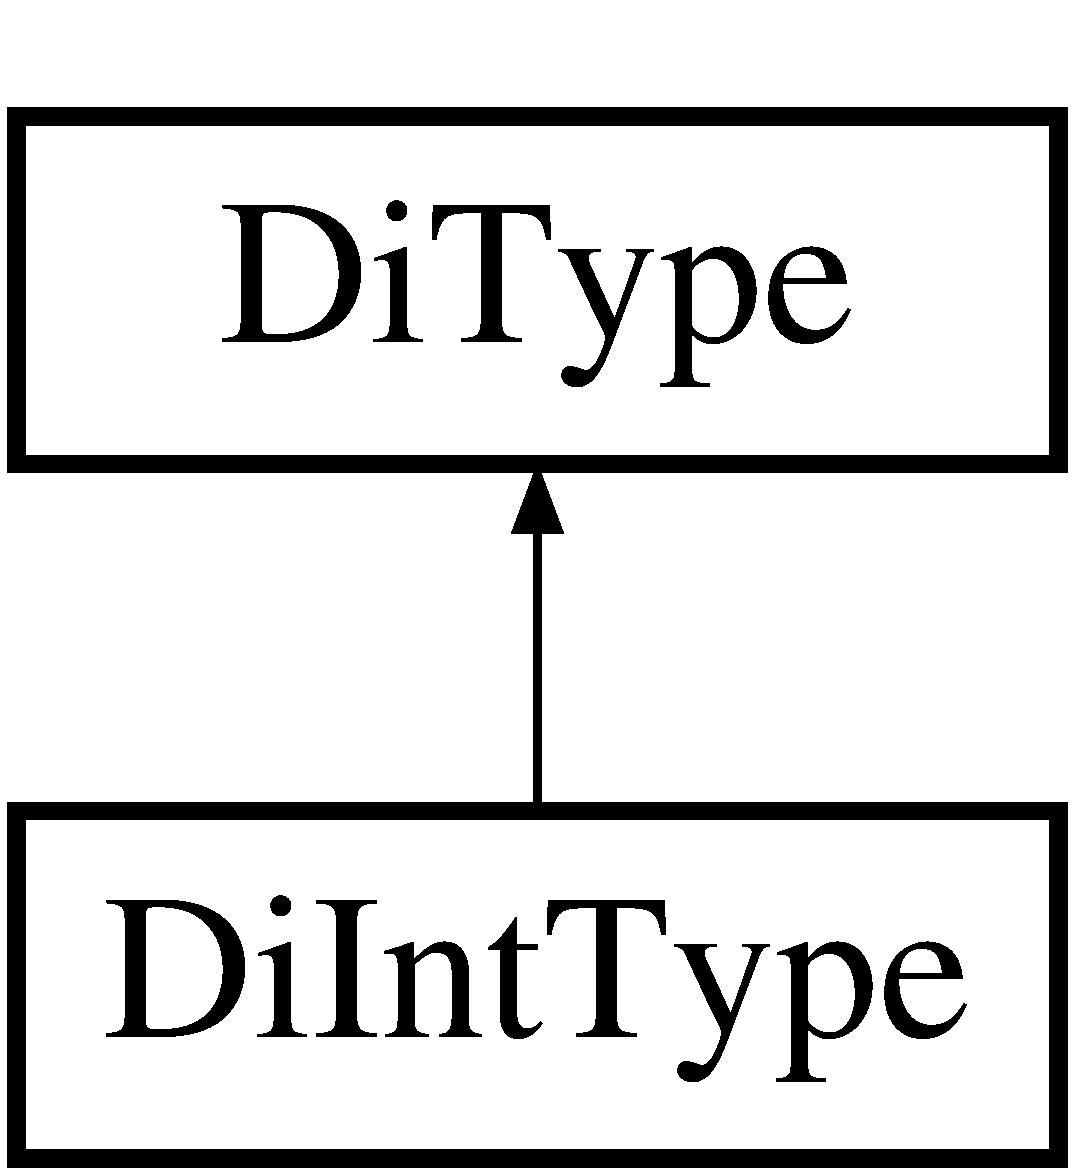
\includegraphics[height=2.000000cm]{class_di_type}
\end{center}
\end{figure}
\subsection*{Public Member Functions}
\begin{DoxyCompactItemize}
\item 
\hyperlink{class_di_type_a8a7f7ce0cd5dbec8798ce3409ff3b01f}{Di\-Type} (B\-Patch\-\_\-image \&bp\-Image, char const $\ast$type\-Name)
\begin{DoxyCompactList}\small\item\em Constructor. \end{DoxyCompactList}\item 
\hypertarget{class_di_type_a76e679b9df26668087c02531ab1f6c54}{{\bfseries operator B\-Patch\-\_\-type \&} ()}\label{class_di_type_a76e679b9df26668087c02531ab1f6c54}

\end{DoxyCompactItemize}


\subsection{Detailed Description}
Dyninst's Type class. It represents a variable or area of memory in a thread's address space. 

\begin{DoxyVersion}{Version}
1.\-0b 
\end{DoxyVersion}
\begin{DoxyAuthor}{Author}
Ania Sikora, 2002 
\end{DoxyAuthor}
\begin{DoxySince}{Since}
1.\-0b 
\end{DoxySince}


\subsection{Constructor \& Destructor Documentation}
\hypertarget{class_di_type_a8a7f7ce0cd5dbec8798ce3409ff3b01f}{\index{Di\-Type@{Di\-Type}!Di\-Type@{Di\-Type}}
\index{Di\-Type@{Di\-Type}!DiType@{Di\-Type}}
\subsubsection[{Di\-Type}]{\setlength{\rightskip}{0pt plus 5cm}Di\-Type\-::\-Di\-Type (
\begin{DoxyParamCaption}
\item[{B\-Patch\-\_\-image \&}]{bp\-Image, }
\item[{char const $\ast$}]{type\-Name}
\end{DoxyParamCaption}
)\hspace{0.3cm}{\ttfamily [inline]}}}\label{class_di_type_a8a7f7ce0cd5dbec8798ce3409ff3b01f}


Constructor. 


\begin{DoxyParams}{Parameters}
{\em bp\-Image} & Image of the program \\
\hline
{\em type\-Name} & Name of the type \\
\hline
\end{DoxyParams}


The documentation for this class was generated from the following file\-:\begin{DoxyCompactItemize}
\item 
Common/di.\-h\end{DoxyCompactItemize}

\hypertarget{class_di_variable}{\section{Di\-Variable Class Reference}
\label{class_di_variable}\index{Di\-Variable@{Di\-Variable}}
}


Deals with Dyninst's Variable class. This can create, read and delete a variable of a given type or size in memory.  




{\ttfamily \#include $<$di.\-h$>$}

Inheritance diagram for Di\-Variable\-:\begin{figure}[H]
\begin{center}
\leavevmode
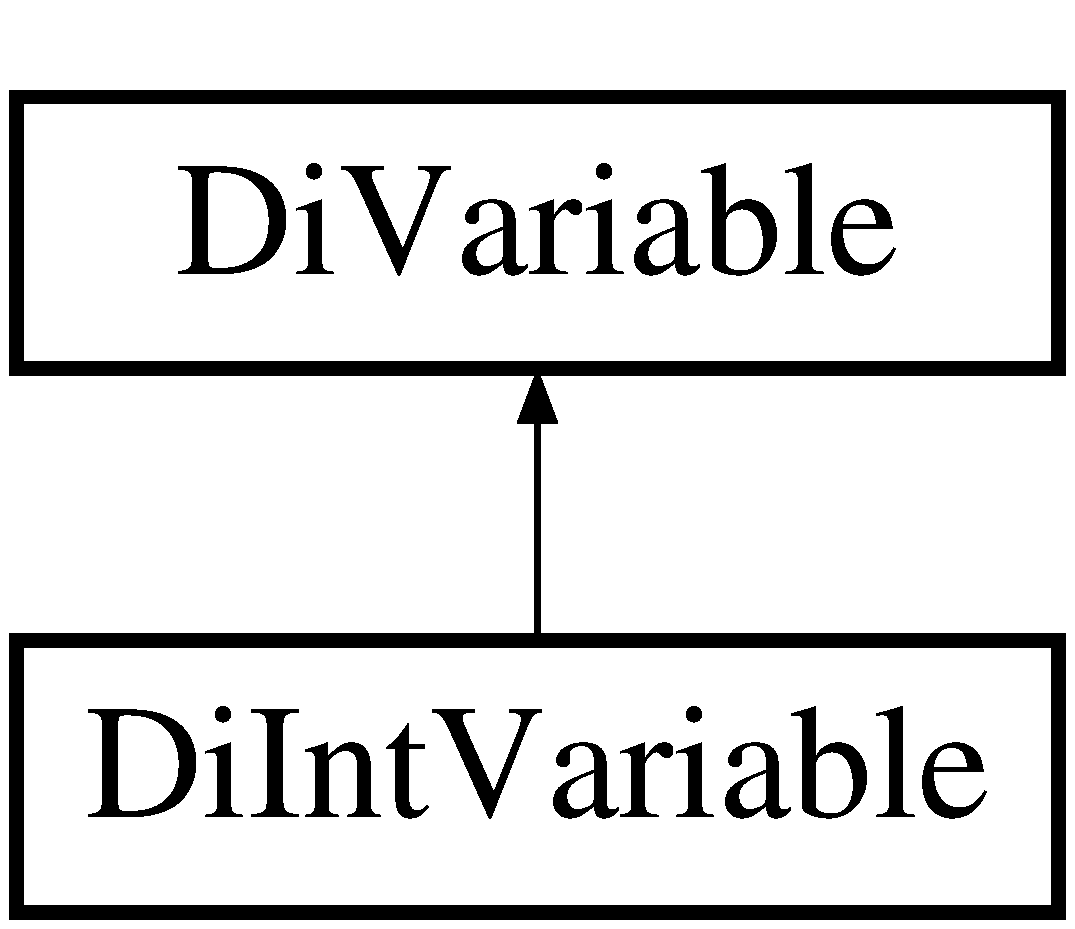
\includegraphics[height=2.000000cm]{class_di_variable}
\end{center}
\end{figure}
\subsection*{Public Member Functions}
\begin{DoxyCompactItemize}
\item 
\hyperlink{class_di_variable_a909e93bc0684f53588b2875c2f6fc3aa}{Di\-Variable} (B\-Patch\-\_\-process \&bp\-Process, B\-Patch\-\_\-type const \&type)
\begin{DoxyCompactList}\small\item\em \hyperlink{class_di_variable}{Di\-Variable} constructor of a given type. \end{DoxyCompactList}\item 
\hyperlink{class_di_variable_ac9b7545cae8d71421296b9e076cb5a42}{Di\-Variable} (B\-Patch\-\_\-process \&bp\-Process, char const $\ast$type\-Name)
\begin{DoxyCompactList}\small\item\em \hyperlink{class_di_variable}{Di\-Variable} constructor of a given type name. \end{DoxyCompactList}\item 
\hyperlink{class_di_variable_ad94dd879a61ffba2dfd3339602ac8d81}{Di\-Variable} (B\-Patch\-\_\-process \&bp\-Process, int size)
\begin{DoxyCompactList}\small\item\em \hyperlink{class_di_variable}{Di\-Variable} constructor of a given size. \end{DoxyCompactList}\item 
\hypertarget{class_di_variable_aacef58e456bbf5a5f74ec678859d4845}{\hyperlink{class_di_variable_aacef58e456bbf5a5f74ec678859d4845}{$\sim$\-Di\-Variable} ()}\label{class_di_variable_aacef58e456bbf5a5f74ec678859d4845}

\begin{DoxyCompactList}\small\item\em Destructor. \end{DoxyCompactList}\item 
\hypertarget{class_di_variable_a06fa020320e2d8852594f17605563522}{{\bfseries operator B\-Patch\-\_\-variable\-Expr \&} ()}\label{class_di_variable_a06fa020320e2d8852594f17605563522}

\item 
\hypertarget{class_di_variable_a8fd67253e046796a14afa17ced1b894c}{{\bfseries operator B\-Patch\-\_\-variable\-Expr $\ast$} ()}\label{class_di_variable_a8fd67253e046796a14afa17ced1b894c}

\item 
void \hyperlink{class_di_variable_a214103cfdd6e36e36ea7f90186450112}{Get\-Value} (void $\ast$dst) const 
\begin{DoxyCompactList}\small\item\em Reads the value of a variable in a thread's address space. $<$dst$>$ is assumed to be the same size as the variable. \end{DoxyCompactList}\item 
long int \hyperlink{class_di_variable_ab75a5f7155896262273505b9f80afab7}{Get\-Address} () const 
\begin{DoxyCompactList}\small\item\em Returns base address of this variable in the target's address space. \end{DoxyCompactList}\end{DoxyCompactItemize}


\subsection{Detailed Description}
Deals with Dyninst's Variable class. This can create, read and delete a variable of a given type or size in memory. 

\begin{DoxyVersion}{Version}
1.\-0b 
\end{DoxyVersion}
\begin{DoxyAuthor}{Author}
Ania Sikora, 2002 
\end{DoxyAuthor}
\begin{DoxySince}{Since}
1.\-0b 
\end{DoxySince}


\subsection{Constructor \& Destructor Documentation}
\hypertarget{class_di_variable_a909e93bc0684f53588b2875c2f6fc3aa}{\index{Di\-Variable@{Di\-Variable}!Di\-Variable@{Di\-Variable}}
\index{Di\-Variable@{Di\-Variable}!DiVariable@{Di\-Variable}}
\subsubsection[{Di\-Variable}]{\setlength{\rightskip}{0pt plus 5cm}Di\-Variable\-::\-Di\-Variable (
\begin{DoxyParamCaption}
\item[{B\-Patch\-\_\-process \&}]{bp\-Process, }
\item[{B\-Patch\-\_\-type const \&}]{type}
\end{DoxyParamCaption}
)\hspace{0.3cm}{\ttfamily [inline]}}}\label{class_di_variable_a909e93bc0684f53588b2875c2f6fc3aa}


\hyperlink{class_di_variable}{Di\-Variable} constructor of a given type. 


\begin{DoxyParams}{Parameters}
{\em bp\-Process} & Process \\
\hline
{\em type} & Type of the variable \\
\hline
\end{DoxyParams}
\hypertarget{class_di_variable_ac9b7545cae8d71421296b9e076cb5a42}{\index{Di\-Variable@{Di\-Variable}!Di\-Variable@{Di\-Variable}}
\index{Di\-Variable@{Di\-Variable}!DiVariable@{Di\-Variable}}
\subsubsection[{Di\-Variable}]{\setlength{\rightskip}{0pt plus 5cm}Di\-Variable\-::\-Di\-Variable (
\begin{DoxyParamCaption}
\item[{B\-Patch\-\_\-process \&}]{bp\-Process, }
\item[{char const $\ast$}]{type\-Name}
\end{DoxyParamCaption}
)\hspace{0.3cm}{\ttfamily [inline]}}}\label{class_di_variable_ac9b7545cae8d71421296b9e076cb5a42}


\hyperlink{class_di_variable}{Di\-Variable} constructor of a given type name. 


\begin{DoxyParams}{Parameters}
{\em bp\-Process} & Process \\
\hline
{\em type\-Name} & Type name \\
\hline
\end{DoxyParams}
\hypertarget{class_di_variable_ad94dd879a61ffba2dfd3339602ac8d81}{\index{Di\-Variable@{Di\-Variable}!Di\-Variable@{Di\-Variable}}
\index{Di\-Variable@{Di\-Variable}!DiVariable@{Di\-Variable}}
\subsubsection[{Di\-Variable}]{\setlength{\rightskip}{0pt plus 5cm}Di\-Variable\-::\-Di\-Variable (
\begin{DoxyParamCaption}
\item[{B\-Patch\-\_\-process \&}]{bp\-Process, }
\item[{int}]{size}
\end{DoxyParamCaption}
)\hspace{0.3cm}{\ttfamily [inline]}}}\label{class_di_variable_ad94dd879a61ffba2dfd3339602ac8d81}


\hyperlink{class_di_variable}{Di\-Variable} constructor of a given size. 


\begin{DoxyParams}{Parameters}
{\em bp\-Process} & Process \\
\hline
{\em size} & Size in bytes \\
\hline
\end{DoxyParams}


\subsection{Member Function Documentation}
\hypertarget{class_di_variable_ab75a5f7155896262273505b9f80afab7}{\index{Di\-Variable@{Di\-Variable}!Get\-Address@{Get\-Address}}
\index{Get\-Address@{Get\-Address}!DiVariable@{Di\-Variable}}
\subsubsection[{Get\-Address}]{\setlength{\rightskip}{0pt plus 5cm}long int Di\-Variable\-::\-Get\-Address (
\begin{DoxyParamCaption}
{}
\end{DoxyParamCaption}
) const\hspace{0.3cm}{\ttfamily [inline]}}}\label{class_di_variable_ab75a5f7155896262273505b9f80afab7}


Returns base address of this variable in the target's address space. 

\begin{DoxyReturn}{Returns}
Base address of the variable 
\end{DoxyReturn}
\hypertarget{class_di_variable_a214103cfdd6e36e36ea7f90186450112}{\index{Di\-Variable@{Di\-Variable}!Get\-Value@{Get\-Value}}
\index{Get\-Value@{Get\-Value}!DiVariable@{Di\-Variable}}
\subsubsection[{Get\-Value}]{\setlength{\rightskip}{0pt plus 5cm}void Di\-Variable\-::\-Get\-Value (
\begin{DoxyParamCaption}
\item[{void $\ast$}]{dst}
\end{DoxyParamCaption}
) const\hspace{0.3cm}{\ttfamily [inline]}}}\label{class_di_variable_a214103cfdd6e36e36ea7f90186450112}


Reads the value of a variable in a thread's address space. $<$dst$>$ is assumed to be the same size as the variable. 


\begin{DoxyParams}{Parameters}
{\em dst} & Reads value from here \\
\hline
\end{DoxyParams}


The documentation for this class was generated from the following file\-:\begin{DoxyCompactItemize}
\item 
Common/di.\-h\end{DoxyCompactItemize}

\hypertarget{class_d_t_library}{\section{D\-T\-Library Class Reference}
\label{class_d_t_library}\index{D\-T\-Library@{D\-T\-Library}}
}


Dynamic Tuning Library that offers D\-T A\-P\-I. Encapsulates information about the application model and the event collector. Provides methods to create application models.  




{\ttfamily \#include $<$D\-T\-A\-P\-I.\-h$>$}

\subsection*{Public Member Functions}
\begin{DoxyCompactItemize}
\item 
\hyperlink{class_model_1_1_application}{Model\-::\-Application} \& \hyperlink{class_d_t_library_a2ab7686b7b3cd67182ae51a35a40810d}{Create\-Application} (char const $\ast$app\-Path, int argc, char const $\ast$$\ast$argv)
\begin{DoxyCompactList}\small\item\em Creates a new application model, a new event collector and associates them. \end{DoxyCompactList}\item 
\hyperlink{class_model_1_1_application}{Model\-::\-Application} \& \hyperlink{class_d_t_library_aa3f99ffaa5e1ca77cf6033e136249ee9}{Get\-Application} ()
\begin{DoxyCompactList}\small\item\em Application getter. \end{DoxyCompactList}\end{DoxyCompactItemize}
\subsection*{Friends}
\begin{DoxyCompactItemize}
\item 
\hypertarget{class_d_t_library_a73d564540d5bff2dc1f0928a4ff776b2}{class {\bfseries D\-T\-Library\-Factory}}\label{class_d_t_library_a73d564540d5bff2dc1f0928a4ff776b2}

\end{DoxyCompactItemize}


\subsection{Detailed Description}
Dynamic Tuning Library that offers D\-T A\-P\-I. Encapsulates information about the application model and the event collector. Provides methods to create application models. 

\subsection{Member Function Documentation}
\hypertarget{class_d_t_library_a2ab7686b7b3cd67182ae51a35a40810d}{\index{D\-T\-Library@{D\-T\-Library}!Create\-Application@{Create\-Application}}
\index{Create\-Application@{Create\-Application}!DTLibrary@{D\-T\-Library}}
\subsubsection[{Create\-Application}]{\setlength{\rightskip}{0pt plus 5cm}{\bf Model\-::\-Application} \& D\-T\-Library\-::\-Create\-Application (
\begin{DoxyParamCaption}
\item[{char const $\ast$}]{app\-Path, }
\item[{int}]{argc, }
\item[{char const $\ast$$\ast$}]{argv}
\end{DoxyParamCaption}
)}}\label{class_d_t_library_a2ab7686b7b3cd67182ae51a35a40810d}


Creates a new application model, a new event collector and associates them. 


\begin{DoxyParams}{Parameters}
{\em app\-Path} & path to the target application. \\
\hline
{\em argc} & number of arguments of the target application. \\
\hline
{\em argv} & list of arguments of the target application.\\
\hline
\end{DoxyParams}
\begin{DoxyReturn}{Returns}
Reference to the application model object. 
\end{DoxyReturn}
\hypertarget{class_d_t_library_aa3f99ffaa5e1ca77cf6033e136249ee9}{\index{D\-T\-Library@{D\-T\-Library}!Get\-Application@{Get\-Application}}
\index{Get\-Application@{Get\-Application}!DTLibrary@{D\-T\-Library}}
\subsubsection[{Get\-Application}]{\setlength{\rightskip}{0pt plus 5cm}{\bf Model\-::\-Application} \& D\-T\-Library\-::\-Get\-Application (
\begin{DoxyParamCaption}
{}
\end{DoxyParamCaption}
)}}\label{class_d_t_library_aa3f99ffaa5e1ca77cf6033e136249ee9}


Application getter. 

\begin{DoxyReturn}{Returns}
Reference to the application model. 
\end{DoxyReturn}


The documentation for this class was generated from the following files\-:\begin{DoxyCompactItemize}
\item 
Analyzer/D\-T\-A\-P\-I.\-h\item 
Analyzer/D\-T\-A\-P\-I.\-cpp\end{DoxyCompactItemize}

\hypertarget{class_d_t_library_factory}{\section{D\-T\-Library\-Factory Class Reference}
\label{class_d_t_library_factory}\index{D\-T\-Library\-Factory@{D\-T\-Library\-Factory}}
}


Handles the creation and destruction of D\-T Libraries.  




{\ttfamily \#include $<$D\-T\-A\-P\-I.\-h$>$}

\subsection*{Static Public Member Functions}
\begin{DoxyCompactItemize}
\item 
static \hyperlink{class_d_t_library}{D\-T\-Library} $\ast$ \hyperlink{class_d_t_library_factory_ab52622245da4d6c4adce2a63da510036}{Create\-Library} (\hyperlink{class_common_1_1_config}{Config} const \&cfg)
\begin{DoxyCompactList}\small\item\em Creates and initializes the D\-T Library. Implements the singleton design pattern, so if the library is already created it returns a reference to it. \end{DoxyCompactList}\item 
static void \hyperlink{class_d_t_library_factory_a4bb94d59eeb3fc6584e9b7c6324b7960}{Destroy\-Library} (\hyperlink{class_d_t_library}{D\-T\-Library} $\ast$lib)
\begin{DoxyCompactList}\small\item\em Destroys the library if there is only one last reference to the object. \end{DoxyCompactList}\end{DoxyCompactItemize}


\subsection{Detailed Description}
Handles the creation and destruction of D\-T Libraries. 

\subsection{Member Function Documentation}
\hypertarget{class_d_t_library_factory_ab52622245da4d6c4adce2a63da510036}{\index{D\-T\-Library\-Factory@{D\-T\-Library\-Factory}!Create\-Library@{Create\-Library}}
\index{Create\-Library@{Create\-Library}!DTLibraryFactory@{D\-T\-Library\-Factory}}
\subsubsection[{Create\-Library}]{\setlength{\rightskip}{0pt plus 5cm}{\bf D\-T\-Library} $\ast$ D\-T\-Library\-Factory\-::\-Create\-Library (
\begin{DoxyParamCaption}
\item[{{\bf Config} const \&}]{cfg}
\end{DoxyParamCaption}
)\hspace{0.3cm}{\ttfamily [static]}}}\label{class_d_t_library_factory_ab52622245da4d6c4adce2a63da510036}


Creates and initializes the D\-T Library. Implements the singleton design pattern, so if the library is already created it returns a reference to it. 


\begin{DoxyParams}{Parameters}
{\em cfg} & Reference to the configuration object.\\
\hline
\end{DoxyParams}
\begin{DoxyReturn}{Returns}
Reference to the library. 
\end{DoxyReturn}
\hypertarget{class_d_t_library_factory_a4bb94d59eeb3fc6584e9b7c6324b7960}{\index{D\-T\-Library\-Factory@{D\-T\-Library\-Factory}!Destroy\-Library@{Destroy\-Library}}
\index{Destroy\-Library@{Destroy\-Library}!DTLibraryFactory@{D\-T\-Library\-Factory}}
\subsubsection[{Destroy\-Library}]{\setlength{\rightskip}{0pt plus 5cm}void D\-T\-Library\-Factory\-::\-Destroy\-Library (
\begin{DoxyParamCaption}
\item[{{\bf D\-T\-Library} $\ast$}]{lib}
\end{DoxyParamCaption}
)\hspace{0.3cm}{\ttfamily [static]}}}\label{class_d_t_library_factory_a4bb94d59eeb3fc6584e9b7c6324b7960}


Destroys the library if there is only one last reference to the object. 


\begin{DoxyParams}{Parameters}
{\em lib} & Reference to the library. \\
\hline
\end{DoxyParams}


The documentation for this class was generated from the following files\-:\begin{DoxyCompactItemize}
\item 
Analyzer/D\-T\-A\-P\-I.\-h\item 
Analyzer/D\-T\-A\-P\-I.\-cpp\end{DoxyCompactItemize}

\hypertarget{class_dyn_inst}{\section{Dyn\-Inst Class Reference}
\label{class_dyn_inst}\index{Dyn\-Inst@{Dyn\-Inst}}
}


Assigns an instance of the class B\-Patch from Dyninst.  




{\ttfamily \#include $<$di.\-h$>$}

\subsection*{Static Public Member Functions}
\begin{DoxyCompactItemize}
\item 
\hypertarget{class_dyn_inst_abc0c0d64809758127d7bb80f3c456a63}{static B\-Patch \& {\bfseries Instance} ()}\label{class_dyn_inst_abc0c0d64809758127d7bb80f3c456a63}

\item 
\hypertarget{class_dyn_inst_a76b3ebe473728291fc999569678dcbe5}{static B\-Patch \& {\bfseries Instance} (B\-Patch in\-\_\-bp)}\label{class_dyn_inst_a76b3ebe473728291fc999569678dcbe5}

\end{DoxyCompactItemize}
\subsection*{Static Protected Member Functions}
\begin{DoxyCompactItemize}
\item 
\hypertarget{class_dyn_inst_a611dbebcb6780fa2427688ecfde8adac}{static void {\bfseries On\-Error} (B\-Patch\-Error\-Level severity, int number, const char $\ast$const $\ast$params)}\label{class_dyn_inst_a611dbebcb6780fa2427688ecfde8adac}

\end{DoxyCompactItemize}


\subsection{Detailed Description}
Assigns an instance of the class B\-Patch from Dyninst. 

\begin{DoxyVersion}{Version}
1.\-0b 
\end{DoxyVersion}
\begin{DoxyAuthor}{Author}
Ania Sikora, 2002 
\end{DoxyAuthor}
\begin{DoxySince}{Since}
1.\-0b 
\end{DoxySince}


The documentation for this class was generated from the following files\-:\begin{DoxyCompactItemize}
\item 
Common/di.\-h\item 
Common/di.\-cpp\end{DoxyCompactItemize}

\hypertarget{class_e_c_p_acceptor}{\section{E\-C\-P\-Acceptor Class Reference}
\label{class_e_c_p_acceptor}\index{E\-C\-P\-Acceptor@{E\-C\-P\-Acceptor}}
}


Event Acceptor class that collects incoming E\-C\-P events and prepares their correspondent handler.  




{\ttfamily \#include $<$Event\-Collector.\-h$>$}

Inheritance diagram for E\-C\-P\-Acceptor\-:\begin{figure}[H]
\begin{center}
\leavevmode
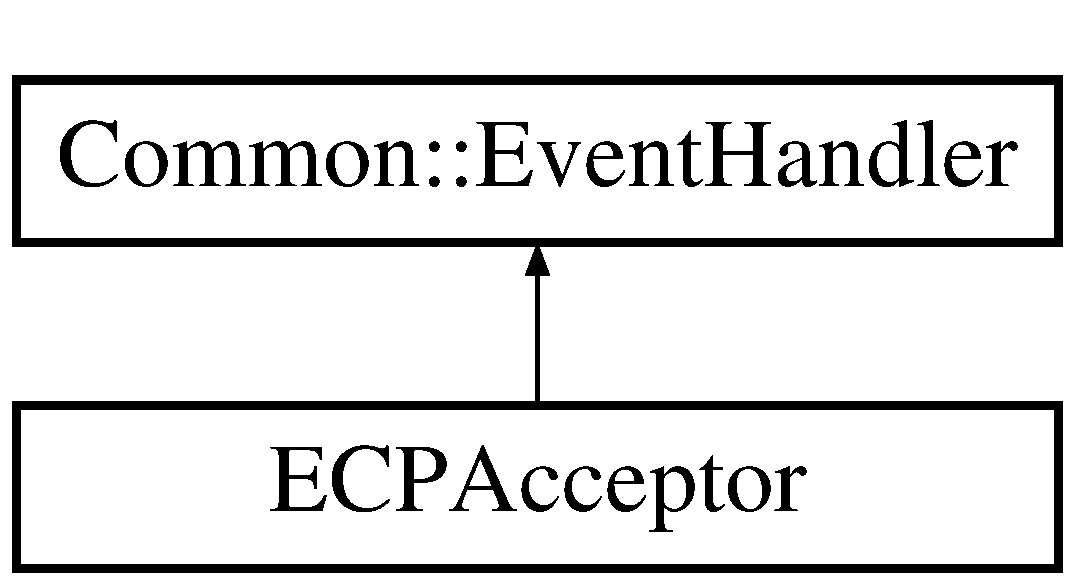
\includegraphics[height=2.000000cm]{class_e_c_p_acceptor}
\end{center}
\end{figure}
\subsection*{Public Member Functions}
\begin{DoxyCompactItemize}
\item 
\hyperlink{class_e_c_p_acceptor_ad0022e1f2544ad417ba49b89336c8f3b}{E\-C\-P\-Acceptor} (\hyperlink{class_common_1_1_reactor}{Reactor} \&reactor, int port)
\begin{DoxyCompactList}\small\item\em Constructor, starts listening to the socket and registers itself in the reactor. \end{DoxyCompactList}\item 
\hypertarget{class_e_c_p_acceptor_aa07b436fe534243a611ee103822a02de}{\hyperlink{class_e_c_p_acceptor_aa07b436fe534243a611ee103822a02de}{$\sim$\-E\-C\-P\-Acceptor} ()}\label{class_e_c_p_acceptor_aa07b436fe534243a611ee103822a02de}

\begin{DoxyCompactList}\small\item\em Destructor, unregister the object from the reactor. \end{DoxyCompactList}\item 
\hypertarget{class_e_c_p_acceptor_afd5c66610d9f62f6c4c40ebeb989167f}{void \hyperlink{class_e_c_p_acceptor_afd5c66610d9f62f6c4c40ebeb989167f}{Handle\-Input} ()}\label{class_e_c_p_acceptor_afd5c66610d9f62f6c4c40ebeb989167f}

\begin{DoxyCompactList}\small\item\em When a new connection is accepted, prepares a handler for it. It is registered in the reactor and added to the service. \end{DoxyCompactList}\item 
int \hyperlink{class_e_c_p_acceptor_a8ab038f08faff45c8e7b1ca77f543c40}{Get\-Handle} ()
\item 
void \hyperlink{class_e_c_p_acceptor_a4f6041e4537d591aa0349e641518e4b3}{Set\-Event\-Collector} (\hyperlink{class_event_collector}{Event\-Collector} $\ast$collector)
\begin{DoxyCompactList}\small\item\em Setter for the event collector. \end{DoxyCompactList}\end{DoxyCompactItemize}


\subsection{Detailed Description}
Event Acceptor class that collects incoming E\-C\-P events and prepares their correspondent handler. 

\subsection{Constructor \& Destructor Documentation}
\hypertarget{class_e_c_p_acceptor_ad0022e1f2544ad417ba49b89336c8f3b}{\index{E\-C\-P\-Acceptor@{E\-C\-P\-Acceptor}!E\-C\-P\-Acceptor@{E\-C\-P\-Acceptor}}
\index{E\-C\-P\-Acceptor@{E\-C\-P\-Acceptor}!ECPAcceptor@{E\-C\-P\-Acceptor}}
\subsubsection[{E\-C\-P\-Acceptor}]{\setlength{\rightskip}{0pt plus 5cm}E\-C\-P\-Acceptor\-::\-E\-C\-P\-Acceptor (
\begin{DoxyParamCaption}
\item[{{\bf Reactor} \&}]{reactor, }
\item[{int}]{port}
\end{DoxyParamCaption}
)}}\label{class_e_c_p_acceptor_ad0022e1f2544ad417ba49b89336c8f3b}


Constructor, starts listening to the socket and registers itself in the reactor. 


\begin{DoxyParams}{Parameters}
{\em reactor} & $\ast$$\ast$ Reactor of the application??? $\ast$$\ast$ \\
\hline
{\em port} & Socket port. \\
\hline
\end{DoxyParams}


\subsection{Member Function Documentation}
\hypertarget{class_e_c_p_acceptor_a8ab038f08faff45c8e7b1ca77f543c40}{\index{E\-C\-P\-Acceptor@{E\-C\-P\-Acceptor}!Get\-Handle@{Get\-Handle}}
\index{Get\-Handle@{Get\-Handle}!ECPAcceptor@{E\-C\-P\-Acceptor}}
\subsubsection[{Get\-Handle}]{\setlength{\rightskip}{0pt plus 5cm}int E\-C\-P\-Acceptor\-::\-Get\-Handle (
\begin{DoxyParamCaption}
{}
\end{DoxyParamCaption}
)\hspace{0.3cm}{\ttfamily [inline]}, {\ttfamily [virtual]}}}\label{class_e_c_p_acceptor_a8ab038f08faff45c8e7b1ca77f543c40}
\begin{DoxyReturn}{Returns}
Reference to the handler object 
\end{DoxyReturn}


Implements \hyperlink{class_common_1_1_event_handler_aaf6cb56038c6fe6b91c9d1e34ee6b3af}{Common\-::\-Event\-Handler}.

\hypertarget{class_e_c_p_acceptor_a4f6041e4537d591aa0349e641518e4b3}{\index{E\-C\-P\-Acceptor@{E\-C\-P\-Acceptor}!Set\-Event\-Collector@{Set\-Event\-Collector}}
\index{Set\-Event\-Collector@{Set\-Event\-Collector}!ECPAcceptor@{E\-C\-P\-Acceptor}}
\subsubsection[{Set\-Event\-Collector}]{\setlength{\rightskip}{0pt plus 5cm}void E\-C\-P\-Acceptor\-::\-Set\-Event\-Collector (
\begin{DoxyParamCaption}
\item[{{\bf Event\-Collector} $\ast$}]{collector}
\end{DoxyParamCaption}
)}}\label{class_e_c_p_acceptor_a4f6041e4537d591aa0349e641518e4b3}


Setter for the event collector. 


\begin{DoxyParams}{Parameters}
{\em collector} & Event collector to be set. \\
\hline
\end{DoxyParams}


The documentation for this class was generated from the following files\-:\begin{DoxyCompactItemize}
\item 
Analyzer/Event\-Collector.\-h\item 
Analyzer/Event\-Collector.\-cpp\end{DoxyCompactItemize}

\hypertarget{class_e_c_p_handler}{\section{E\-C\-P\-Handler Class Reference}
\label{class_e_c_p_handler}\index{E\-C\-P\-Handler@{E\-C\-P\-Handler}}
}


Encapsulates data structures and methods to handle incoming event collector inputs.  




{\ttfamily \#include $<$E\-C\-P\-Handler.\-h$>$}

Inheritance diagram for E\-C\-P\-Handler\-:\begin{figure}[H]
\begin{center}
\leavevmode
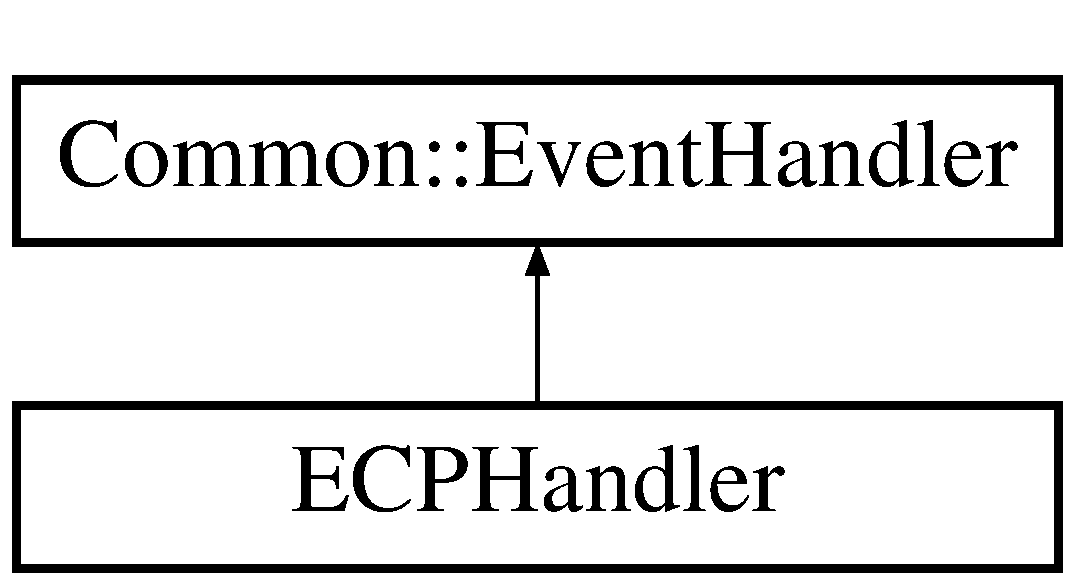
\includegraphics[height=2.000000cm]{class_e_c_p_handler}
\end{center}
\end{figure}
\subsection*{Public Member Functions}
\begin{DoxyCompactItemize}
\item 
\hypertarget{class_e_c_p_handler_abbb4765085c0b0e68882474214bd0336}{\hyperlink{class_e_c_p_handler_abbb4765085c0b0e68882474214bd0336}{E\-C\-P\-Handler} (Socket\-Ptr \&socket, \hyperlink{class_event_collector}{Event\-Collector} $\ast$collector)}\label{class_e_c_p_handler_abbb4765085c0b0e68882474214bd0336}

\begin{DoxyCompactList}\small\item\em Constructor. \end{DoxyCompactList}\item 
\hypertarget{class_e_c_p_handler_ac6fd0bc755f3dfe4bbac87c5c2be28be}{void \hyperlink{class_e_c_p_handler_ac6fd0bc755f3dfe4bbac87c5c2be28be}{Remove} ()}\label{class_e_c_p_handler_ac6fd0bc755f3dfe4bbac87c5c2be28be}

\begin{DoxyCompactList}\small\item\em Not implemented (here for compatibility reasons) \end{DoxyCompactList}\item 
\hypertarget{class_e_c_p_handler_ac0ca3a32612f0afc1323af8eb2af82c8}{void \hyperlink{class_e_c_p_handler_ac0ca3a32612f0afc1323af8eb2af82c8}{Handle\-Input} ()}\label{class_e_c_p_handler_ac0ca3a32612f0afc1323af8eb2af82c8}

\begin{DoxyCompactList}\small\item\em Reads an incoming message and handles it depending on its type. First reads a message from the socket, then creates the proper type of message and the calls the on\-Event method of the listener of the events (if any). \end{DoxyCompactList}\item 
int \hyperlink{class_e_c_p_handler_aae9a377a352483804795117312a72544}{Get\-Handle} ()
\begin{DoxyCompactList}\small\item\em Handler getter. \end{DoxyCompactList}\item 
void \hyperlink{class_e_c_p_handler_a52c29fb21cd3e665dc45a60bf55f2ed0}{Set\-Service} (\hyperlink{class_service}{Service} $\ast$service)
\begin{DoxyCompactList}\small\item\em \hyperlink{class_service}{Service} setter. \end{DoxyCompactList}\end{DoxyCompactItemize}


\subsection{Detailed Description}
Encapsulates data structures and methods to handle incoming event collector inputs. 

\subsection{Member Function Documentation}
\hypertarget{class_e_c_p_handler_aae9a377a352483804795117312a72544}{\index{E\-C\-P\-Handler@{E\-C\-P\-Handler}!Get\-Handle@{Get\-Handle}}
\index{Get\-Handle@{Get\-Handle}!ECPHandler@{E\-C\-P\-Handler}}
\subsubsection[{Get\-Handle}]{\setlength{\rightskip}{0pt plus 5cm}int E\-C\-P\-Handler\-::\-Get\-Handle (
\begin{DoxyParamCaption}
{}
\end{DoxyParamCaption}
)\hspace{0.3cm}{\ttfamily [inline]}, {\ttfamily [virtual]}}}\label{class_e_c_p_handler_aae9a377a352483804795117312a72544}


Handler getter. 

\begin{DoxyReturn}{Returns}
Reference to the handler object 
\end{DoxyReturn}


Implements \hyperlink{class_common_1_1_event_handler_aaf6cb56038c6fe6b91c9d1e34ee6b3af}{Common\-::\-Event\-Handler}.

\hypertarget{class_e_c_p_handler_a52c29fb21cd3e665dc45a60bf55f2ed0}{\index{E\-C\-P\-Handler@{E\-C\-P\-Handler}!Set\-Service@{Set\-Service}}
\index{Set\-Service@{Set\-Service}!ECPHandler@{E\-C\-P\-Handler}}
\subsubsection[{Set\-Service}]{\setlength{\rightskip}{0pt plus 5cm}void E\-C\-P\-Handler\-::\-Set\-Service (
\begin{DoxyParamCaption}
\item[{{\bf Service} $\ast$}]{service}
\end{DoxyParamCaption}
)\hspace{0.3cm}{\ttfamily [inline]}}}\label{class_e_c_p_handler_a52c29fb21cd3e665dc45a60bf55f2ed0}


\hyperlink{class_service}{Service} setter. 


\begin{DoxyParams}{Parameters}
{\em service} & Reference to the service. \\
\hline
\end{DoxyParams}


The documentation for this class was generated from the following files\-:\begin{DoxyCompactItemize}
\item 
Analyzer/E\-C\-P\-Handler.\-h\item 
Analyzer/E\-C\-P\-Handler.\-cpp\end{DoxyCompactItemize}

\hypertarget{class_common_1_1_e_c_p_message}{\section{Common\-:\-:E\-C\-P\-Message Class Reference}
\label{class_common_1_1_e_c_p_message}\index{Common\-::\-E\-C\-P\-Message@{Common\-::\-E\-C\-P\-Message}}
}


Abstract class, Event\-Collector\-Protocol, represents message interchanged between D\-M\-Lib and analyzer.  




{\ttfamily \#include $<$E\-C\-P\-Msg.\-h$>$}

Inheritance diagram for Common\-:\-:E\-C\-P\-Message\-:\begin{figure}[H]
\begin{center}
\leavevmode
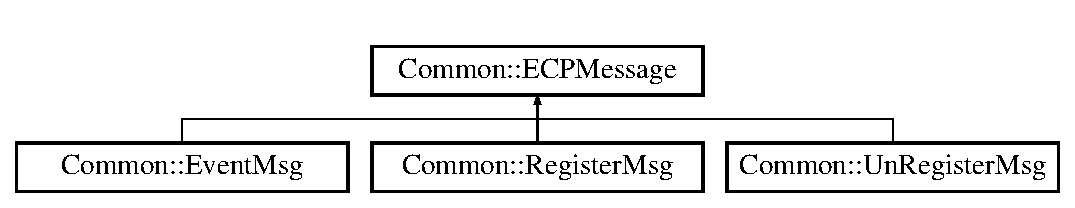
\includegraphics[height=2.000000cm]{class_common_1_1_e_c_p_message}
\end{center}
\end{figure}
\subsection*{Public Member Functions}
\begin{DoxyCompactItemize}
\item 
\hypertarget{class_common_1_1_e_c_p_message_ab89759d2977bde718b296573c308e1a0}{virtual E\-C\-P\-Msg\-Type \hyperlink{class_common_1_1_e_c_p_message_ab89759d2977bde718b296573c308e1a0}{Get\-Type} () const =0}\label{class_common_1_1_e_c_p_message_ab89759d2977bde718b296573c308e1a0}

\begin{DoxyCompactList}\small\item\em To be implemented by subclasses. \end{DoxyCompactList}\item 
\hypertarget{class_common_1_1_e_c_p_message_a9de0bc0ffea7a980b4f938d753c1e9f4}{virtual int \hyperlink{class_common_1_1_e_c_p_message_a9de0bc0ffea7a980b4f938d753c1e9f4}{Get\-Data\-Size} () const }\label{class_common_1_1_e_c_p_message_a9de0bc0ffea7a980b4f938d753c1e9f4}

\begin{DoxyCompactList}\small\item\em Returns size of the data once serialized. \end{DoxyCompactList}\item 
\hypertarget{class_common_1_1_e_c_p_message_a9288d23442703c5a58b8e56e0dd9ca53}{virtual void \hyperlink{class_common_1_1_e_c_p_message_a9288d23442703c5a58b8e56e0dd9ca53}{Serialize} (\hyperlink{class_common_1_1_serializer}{Serializer} \&out) const =0}\label{class_common_1_1_e_c_p_message_a9288d23442703c5a58b8e56e0dd9ca53}

\begin{DoxyCompactList}\small\item\em To be implemented by subclasses. \end{DoxyCompactList}\item 
\hypertarget{class_common_1_1_e_c_p_message_afed137550ebd758400d93f7e9e019a44}{virtual void \hyperlink{class_common_1_1_e_c_p_message_afed137550ebd758400d93f7e9e019a44}{De\-Serialize} (\hyperlink{class_common_1_1_de_serializer}{De\-Serializer} \&in)=0}\label{class_common_1_1_e_c_p_message_afed137550ebd758400d93f7e9e019a44}

\begin{DoxyCompactList}\small\item\em To be implemented by subclasses. \end{DoxyCompactList}\end{DoxyCompactItemize}
\subsection*{Protected Member Functions}
\begin{DoxyCompactItemize}
\item 
\hyperlink{class_common_1_1_e_c_p_message_a934360feea8d6cd1500810b7c17c168b}{E\-C\-P\-Message} ()
\begin{DoxyCompactList}\small\item\em Constructor. \end{DoxyCompactList}\end{DoxyCompactItemize}


\subsection{Detailed Description}
Abstract class, Event\-Collector\-Protocol, represents message interchanged between D\-M\-Lib and analyzer. 

\begin{DoxyVersion}{Version}
1.\-0b 
\end{DoxyVersion}
\begin{DoxySince}{Since}
1.\-0b 
\end{DoxySince}
\begin{DoxyAuthor}{Author}
Ania Sikora, 2002 
\end{DoxyAuthor}


\subsection{Constructor \& Destructor Documentation}
\hypertarget{class_common_1_1_e_c_p_message_a934360feea8d6cd1500810b7c17c168b}{\index{Common\-::\-E\-C\-P\-Message@{Common\-::\-E\-C\-P\-Message}!E\-C\-P\-Message@{E\-C\-P\-Message}}
\index{E\-C\-P\-Message@{E\-C\-P\-Message}!Common::ECPMessage@{Common\-::\-E\-C\-P\-Message}}
\subsubsection[{E\-C\-P\-Message}]{\setlength{\rightskip}{0pt plus 5cm}Common\-::\-E\-C\-P\-Message\-::\-E\-C\-P\-Message (
\begin{DoxyParamCaption}
{}
\end{DoxyParamCaption}
)\hspace{0.3cm}{\ttfamily [inline]}, {\ttfamily [protected]}}}\label{class_common_1_1_e_c_p_message_a934360feea8d6cd1500810b7c17c168b}


Constructor. 

Protected so that this base class cannot be explicitly instantiated. 

The documentation for this class was generated from the following files\-:\begin{DoxyCompactItemize}
\item 
Common/E\-C\-P\-Msg.\-h\item 
Common/E\-C\-P\-Msg.\-cpp\end{DoxyCompactItemize}

\hypertarget{class_common_1_1_e_c_p_msg_header}{\section{Common\-:\-:E\-C\-P\-Msg\-Header Class Reference}
\label{class_common_1_1_e_c_p_msg_header}\index{Common\-::\-E\-C\-P\-Msg\-Header@{Common\-::\-E\-C\-P\-Msg\-Header}}
}


Represents header of an \hyperlink{class_common_1_1_e_c_p_message}{E\-C\-P\-Message} object.  




{\ttfamily \#include $<$E\-C\-P\-Msg\-Header.\-h$>$}

Inheritance diagram for Common\-:\-:E\-C\-P\-Msg\-Header\-:\begin{figure}[H]
\begin{center}
\leavevmode
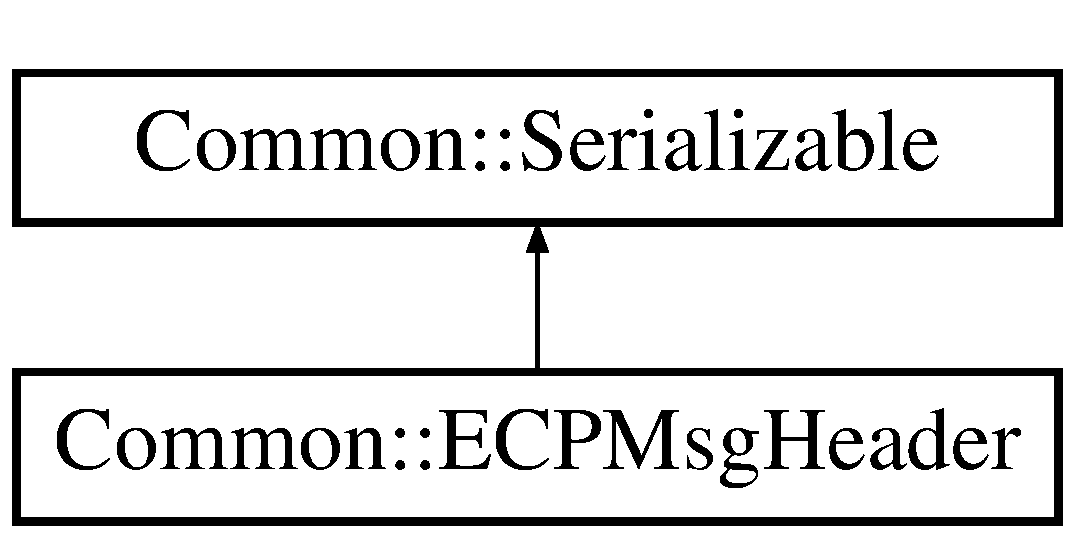
\includegraphics[height=2.000000cm]{class_common_1_1_e_c_p_msg_header}
\end{center}
\end{figure}
\subsection*{Public Member Functions}
\begin{DoxyCompactItemize}
\item 
\hypertarget{class_common_1_1_e_c_p_msg_header_ab217fae80bb79e87cf7d4aa12e7175cb}{\hyperlink{class_common_1_1_e_c_p_msg_header_ab217fae80bb79e87cf7d4aa12e7175cb}{E\-C\-P\-Msg\-Header} ()}\label{class_common_1_1_e_c_p_msg_header_ab217fae80bb79e87cf7d4aa12e7175cb}

\begin{DoxyCompactList}\small\item\em Constructor. \end{DoxyCompactList}\item 
\hypertarget{class_common_1_1_e_c_p_msg_header_a900b44a6a9855c332ee967b3e15e3806}{void \hyperlink{class_common_1_1_e_c_p_msg_header_a900b44a6a9855c332ee967b3e15e3806}{Serialize} (\hyperlink{class_common_1_1_serializer}{Serializer} \&out) const }\label{class_common_1_1_e_c_p_msg_header_a900b44a6a9855c332ee967b3e15e3806}

\begin{DoxyCompactList}\small\item\em Sends the message header. \end{DoxyCompactList}\item 
\hypertarget{class_common_1_1_e_c_p_msg_header_af3c24a86eda3d3bdf66a565cab761406}{void \hyperlink{class_common_1_1_e_c_p_msg_header_af3c24a86eda3d3bdf66a565cab761406}{De\-Serialize} (\hyperlink{class_common_1_1_de_serializer}{De\-Serializer} \&in)}\label{class_common_1_1_e_c_p_msg_header_af3c24a86eda3d3bdf66a565cab761406}

\begin{DoxyCompactList}\small\item\em Receives the message header. \end{DoxyCompactList}\item 
\hypertarget{class_common_1_1_e_c_p_msg_header_aa3949f00cb45d7a958993b4ba1d92e86}{int \hyperlink{class_common_1_1_e_c_p_msg_header_aa3949f00cb45d7a958993b4ba1d92e86}{Get\-Magic} () const }\label{class_common_1_1_e_c_p_msg_header_aa3949f00cb45d7a958993b4ba1d92e86}

\begin{DoxyCompactList}\small\item\em Returns magic attribute. \end{DoxyCompactList}\item 
\hypertarget{class_common_1_1_e_c_p_msg_header_a80a0cb0910c2d0e516bd059ef2869f8f}{int \hyperlink{class_common_1_1_e_c_p_msg_header_a80a0cb0910c2d0e516bd059ef2869f8f}{Get\-Version} () const }\label{class_common_1_1_e_c_p_msg_header_a80a0cb0910c2d0e516bd059ef2869f8f}

\begin{DoxyCompactList}\small\item\em Returns version attribute. \end{DoxyCompactList}\item 
\hypertarget{class_common_1_1_e_c_p_msg_header_ae62210fa06b76aa75c140facd7ae85ff}{E\-C\-P\-Msg\-Type \hyperlink{class_common_1_1_e_c_p_msg_header_ae62210fa06b76aa75c140facd7ae85ff}{Get\-Type} () const }\label{class_common_1_1_e_c_p_msg_header_ae62210fa06b76aa75c140facd7ae85ff}

\begin{DoxyCompactList}\small\item\em Returns type of the message. \end{DoxyCompactList}\item 
\hypertarget{class_common_1_1_e_c_p_msg_header_aa712ed9537812d42d1ce52fff6104c2e}{int \hyperlink{class_common_1_1_e_c_p_msg_header_aa712ed9537812d42d1ce52fff6104c2e}{Get\-Data\-Size} () const }\label{class_common_1_1_e_c_p_msg_header_aa712ed9537812d42d1ce52fff6104c2e}

\begin{DoxyCompactList}\small\item\em Returns data size. \end{DoxyCompactList}\item 
\hypertarget{class_common_1_1_e_c_p_msg_header_a2ff0d80bb4ba8656351e251729f5d3fd}{int \hyperlink{class_common_1_1_e_c_p_msg_header_a2ff0d80bb4ba8656351e251729f5d3fd}{Get\-Header\-Size} () const }\label{class_common_1_1_e_c_p_msg_header_a2ff0d80bb4ba8656351e251729f5d3fd}

\begin{DoxyCompactList}\small\item\em Returns header size. \end{DoxyCompactList}\item 
\hypertarget{class_common_1_1_e_c_p_msg_header_af68784a07eca799d8d8cc1239a5d8eb3}{void \hyperlink{class_common_1_1_e_c_p_msg_header_af68784a07eca799d8d8cc1239a5d8eb3}{Set\-Magic} (int magic)}\label{class_common_1_1_e_c_p_msg_header_af68784a07eca799d8d8cc1239a5d8eb3}

\begin{DoxyCompactList}\small\item\em Sets magic attribute. \end{DoxyCompactList}\item 
\hypertarget{class_common_1_1_e_c_p_msg_header_a23e0b19f8ad3e9433ed145177115c9fa}{void \hyperlink{class_common_1_1_e_c_p_msg_header_a23e0b19f8ad3e9433ed145177115c9fa}{Set\-Version} (int version)}\label{class_common_1_1_e_c_p_msg_header_a23e0b19f8ad3e9433ed145177115c9fa}

\begin{DoxyCompactList}\small\item\em Sets version attribute. \end{DoxyCompactList}\item 
\hypertarget{class_common_1_1_e_c_p_msg_header_a9ac66458c65b4f049f70cae4aefbf6a0}{void \hyperlink{class_common_1_1_e_c_p_msg_header_a9ac66458c65b4f049f70cae4aefbf6a0}{Set\-Msg\-Type} (E\-C\-P\-Msg\-Type type)}\label{class_common_1_1_e_c_p_msg_header_a9ac66458c65b4f049f70cae4aefbf6a0}

\begin{DoxyCompactList}\small\item\em Sets type attribute. \end{DoxyCompactList}\item 
\hypertarget{class_common_1_1_e_c_p_msg_header_a799c73f11ac069ab79d42d03137bc341}{void \hyperlink{class_common_1_1_e_c_p_msg_header_a799c73f11ac069ab79d42d03137bc341}{Set\-Data\-Size} (int size)}\label{class_common_1_1_e_c_p_msg_header_a799c73f11ac069ab79d42d03137bc341}

\begin{DoxyCompactList}\small\item\em Sets the data size attribute. \end{DoxyCompactList}\item 
\hypertarget{class_common_1_1_e_c_p_msg_header_a11971a2c7551b939d5620969946f0169}{void \hyperlink{class_common_1_1_e_c_p_msg_header_a11971a2c7551b939d5620969946f0169}{Set\-Header\-Size} ()}\label{class_common_1_1_e_c_p_msg_header_a11971a2c7551b939d5620969946f0169}

\begin{DoxyCompactList}\small\item\em Updates header size. \end{DoxyCompactList}\end{DoxyCompactItemize}


\subsection{Detailed Description}
Represents header of an \hyperlink{class_common_1_1_e_c_p_message}{E\-C\-P\-Message} object. 

\begin{DoxyVersion}{Version}
1.\-0b 
\end{DoxyVersion}
\begin{DoxySince}{Since}
1.\-0b 
\end{DoxySince}
\begin{DoxyAuthor}{Author}
Ania Sikora, 2002 
\end{DoxyAuthor}


The documentation for this class was generated from the following files\-:\begin{DoxyCompactItemize}
\item 
Common/E\-C\-P\-Msg\-Header.\-h\item 
Common/E\-C\-P\-Msg\-Header.\-cpp\end{DoxyCompactItemize}

\hypertarget{class_e_c_p_protocol}{\section{E\-C\-P\-Protocol Class Reference}
\label{class_e_c_p_protocol}\index{E\-C\-P\-Protocol@{E\-C\-P\-Protocol}}
}


Encapsulates methods to read and handle incoming network messages.  




{\ttfamily \#include $<$E\-C\-P\-Protocol.\-h$>$}

\subsection*{Static Public Member Functions}
\begin{DoxyCompactItemize}
\item 
static \hyperlink{class_common_1_1_e_c_p_msg_header}{E\-C\-P\-Msg\-Header} \hyperlink{class_e_c_p_protocol_a455f930ac9dcda3574bc0c90e0db7a73}{Read\-Message\-Header} (\hyperlink{class_common_1_1_socket}{Socket} \&sock)
\begin{DoxyCompactList}\small\item\em Reads a message header from the socket, deserializes it and creates a message header object. \end{DoxyCompactList}\item 
static \hyperlink{class_common_1_1_e_c_p_message}{E\-C\-P\-Message} $\ast$ \hyperlink{class_e_c_p_protocol_ab6105325b469aab2c38841cc5c285f31}{Read\-Message\-Ex} (\hyperlink{class_common_1_1_socket}{Socket} \&sock)
\begin{DoxyCompactList}\small\item\em Reads a message from the socket, deserializes it and creates different kind of message objects depending on their type. \end{DoxyCompactList}\end{DoxyCompactItemize}


\subsection{Detailed Description}
Encapsulates methods to read and handle incoming network messages. 

\subsection{Member Function Documentation}
\hypertarget{class_e_c_p_protocol_ab6105325b469aab2c38841cc5c285f31}{\index{E\-C\-P\-Protocol@{E\-C\-P\-Protocol}!Read\-Message\-Ex@{Read\-Message\-Ex}}
\index{Read\-Message\-Ex@{Read\-Message\-Ex}!ECPProtocol@{E\-C\-P\-Protocol}}
\subsubsection[{Read\-Message\-Ex}]{\setlength{\rightskip}{0pt plus 5cm}{\bf E\-C\-P\-Message} $\ast$ E\-C\-P\-Protocol\-::\-Read\-Message\-Ex (
\begin{DoxyParamCaption}
\item[{{\bf Socket} \&}]{sock}
\end{DoxyParamCaption}
)\hspace{0.3cm}{\ttfamily [static]}}}\label{class_e_c_p_protocol_ab6105325b469aab2c38841cc5c285f31}


Reads a message from the socket, deserializes it and creates different kind of message objects depending on their type. 


\begin{DoxyParams}{Parameters}
{\em sock} & Reference to the socket.\\
\hline
\end{DoxyParams}
\begin{DoxyReturn}{Returns}
Reference to the message object created. 
\end{DoxyReturn}
\hypertarget{class_e_c_p_protocol_a455f930ac9dcda3574bc0c90e0db7a73}{\index{E\-C\-P\-Protocol@{E\-C\-P\-Protocol}!Read\-Message\-Header@{Read\-Message\-Header}}
\index{Read\-Message\-Header@{Read\-Message\-Header}!ECPProtocol@{E\-C\-P\-Protocol}}
\subsubsection[{Read\-Message\-Header}]{\setlength{\rightskip}{0pt plus 5cm}{\bf E\-C\-P\-Msg\-Header} E\-C\-P\-Protocol\-::\-Read\-Message\-Header (
\begin{DoxyParamCaption}
\item[{{\bf Socket} \&}]{sock}
\end{DoxyParamCaption}
)\hspace{0.3cm}{\ttfamily [static]}}}\label{class_e_c_p_protocol_a455f930ac9dcda3574bc0c90e0db7a73}


Reads a message header from the socket, deserializes it and creates a message header object. 


\begin{DoxyParams}{Parameters}
{\em sock} & Reference to the socket.\\
\hline
\end{DoxyParams}
\begin{DoxyReturn}{Returns}
Reference to the message header object created 
\end{DoxyReturn}


The documentation for this class was generated from the following files\-:\begin{DoxyCompactItemize}
\item 
Analyzer/E\-C\-P\-Protocol.\-h\item 
Analyzer/E\-C\-P\-Protocol.\-cpp\end{DoxyCompactItemize}

\hypertarget{class_model_1_1_event}{\section{Model\-:\-:Event Class Reference}
\label{class_model_1_1_event}\index{Model\-::\-Event@{Model\-::\-Event}}
}


Encapsulates information about the events that the target application generates. For each event holds identification information (id, name), the place where it is produced, its attributes (for example the parameters of a function) and a reference to a handler. As this is a model class the methods provided are for accessing and setting the members of the data structure.  




{\ttfamily \#include $<$App\-Event.\-h$>$}

\subsection*{Public Member Functions}
\begin{DoxyCompactItemize}
\item 
\hyperlink{class_model_1_1_event_afcfebfa23d6c60c3632528aa58805617}{Event} (\hyperlink{class_model_1_1_event}{Event} const \&e)
\begin{DoxyCompactList}\small\item\em Copy constructor. \end{DoxyCompactList}\item 
\hyperlink{class_model_1_1_event_a0f311fa972df39b141bfdb8291f9d477}{Event} (int id, std\-::string const \&func\-Name, Instr\-Place place)
\begin{DoxyCompactList}\small\item\em Constructor. \end{DoxyCompactList}\item 
\hypertarget{class_model_1_1_event_a7704ec01ce91e673885792054214b3d2}{\hyperlink{class_model_1_1_event_a7704ec01ce91e673885792054214b3d2}{$\sim$\-Event} ()}\label{class_model_1_1_event_a7704ec01ce91e673885792054214b3d2}

\begin{DoxyCompactList}\small\item\em Destructor. \end{DoxyCompactList}\item 
int \hyperlink{class_model_1_1_event_ac7b7d9607b8ea5c1ac0300120ad05807}{Get\-Id} () const 
\begin{DoxyCompactList}\small\item\em Globally unique event id getter. \end{DoxyCompactList}\item 
string \hyperlink{class_model_1_1_event_a341b241b108db5bda1f388a2d3379047}{Get\-Function\-Name} () const 
\begin{DoxyCompactList}\small\item\em Name getter. \end{DoxyCompactList}\item 
Instr\-Place \hyperlink{class_model_1_1_event_ab94faa4d80aac8a3bb0e580944fcc023}{Get\-Instr\-Place} () const 
\begin{DoxyCompactList}\small\item\em Instruction place getter. \end{DoxyCompactList}\item 
int \hyperlink{class_model_1_1_event_a01daa5713432336487fce34d87fd1cc9}{Get\-Num\-Attributes} () const 
\begin{DoxyCompactList}\small\item\em Number of attributes getter. \end{DoxyCompactList}\item 
\hyperlink{class_common_1_1_attribute}{Attribute} $\ast$ \hyperlink{class_model_1_1_event_a90a9468086e076656f1bc910dbcb7a3f}{Get\-Attributes} () const 
\begin{DoxyCompactList}\small\item\em Attributes getter. \end{DoxyCompactList}\item 
void \hyperlink{class_model_1_1_event_a22ee34f5b6028817a1b3175799c64ec2}{Set\-Attribute} (int n\-Attrs, \hyperlink{class_common_1_1_attribute}{Attribute} $\ast$attrs)
\begin{DoxyCompactList}\small\item\em Attributes setter. \end{DoxyCompactList}\item 
void \hyperlink{class_model_1_1_event_a9ff45caab649bc7dda897385e715596f}{Set\-N\-Events} (int n\-Events)
\begin{DoxyCompactList}\small\item\em Attributes setter. \end{DoxyCompactList}\item 
void \hyperlink{class_model_1_1_event_a326a936a45b9a0923c8d6cc1ae99839e}{Set\-Event\-Handler} (\hyperlink{class_model_1_1_event_handler}{Event\-Handler} \&h)
\begin{DoxyCompactList}\small\item\em Installs a callback function that is called each time a record of this event is delivered. \end{DoxyCompactList}\item 
\hyperlink{class_model_1_1_event_handler}{Event\-Handler} $\ast$ \hyperlink{class_model_1_1_event_a4ccaa201a88d5134e41d5fc94af2063b}{Get\-Event\-Handler} ()
\begin{DoxyCompactList}\small\item\em \hyperlink{class_model_1_1_event}{Event} handler getter. \end{DoxyCompactList}\item 
int \hyperlink{class_model_1_1_event_a246ade8614bdf20a642573280518ce0c}{Get\-N\-Events} () const 
\begin{DoxyCompactList}\small\item\em Number of Papi metrics getter. \end{DoxyCompactList}\item 
int \hyperlink{class_model_1_1_event_a87c4fcf12c67448d5d9d1df8c43f90e5}{Get\-Num\-Papi\-Metrics} () const 
\begin{DoxyCompactList}\small\item\em Number of Papi metrics getter. \end{DoxyCompactList}\item 
\hypertarget{class_model_1_1_event_a99f40ff3240bde174c92e07228a208dc}{std\-::string $\ast$ {\bfseries Get\-Metrics} () const }\label{class_model_1_1_event_a99f40ff3240bde174c92e07228a208dc}

\item 
\hypertarget{class_model_1_1_event_a00e550f2db2bea0bab4632103e4a470e}{void {\bfseries Set\-Metric} (int n\-Papi, std\-::string $\ast$Papi\-Metrics)}\label{class_model_1_1_event_a00e550f2db2bea0bab4632103e4a470e}

\end{DoxyCompactItemize}


\subsection{Detailed Description}
Encapsulates information about the events that the target application generates. For each event holds identification information (id, name), the place where it is produced, its attributes (for example the parameters of a function) and a reference to a handler. As this is a model class the methods provided are for accessing and setting the members of the data structure. 

\subsection{Constructor \& Destructor Documentation}
\hypertarget{class_model_1_1_event_afcfebfa23d6c60c3632528aa58805617}{\index{Model\-::\-Event@{Model\-::\-Event}!Event@{Event}}
\index{Event@{Event}!Model::Event@{Model\-::\-Event}}
\subsubsection[{Event}]{\setlength{\rightskip}{0pt plus 5cm}Event\-::\-Event (
\begin{DoxyParamCaption}
\item[{{\bf Event} const \&}]{e}
\end{DoxyParamCaption}
)}}\label{class_model_1_1_event_afcfebfa23d6c60c3632528aa58805617}


Copy constructor. 


\begin{DoxyParams}{Parameters}
{\em e} & the event to copy \\
\hline
\end{DoxyParams}
\hypertarget{class_model_1_1_event_a0f311fa972df39b141bfdb8291f9d477}{\index{Model\-::\-Event@{Model\-::\-Event}!Event@{Event}}
\index{Event@{Event}!Model::Event@{Model\-::\-Event}}
\subsubsection[{Event}]{\setlength{\rightskip}{0pt plus 5cm}Event\-::\-Event (
\begin{DoxyParamCaption}
\item[{int}]{id, }
\item[{std\-::string const \&}]{func\-Name, }
\item[{Instr\-Place}]{place}
\end{DoxyParamCaption}
)}}\label{class_model_1_1_event_a0f311fa972df39b141bfdb8291f9d477}


Constructor. 


\begin{DoxyParams}{Parameters}
{\em id} & unique identification number for the event \\
\hline
{\em func\-Name} & name of the function which the event is associated to \\
\hline
{\em place} & place of the function \\
\hline
\end{DoxyParams}


\subsection{Member Function Documentation}
\hypertarget{class_model_1_1_event_a90a9468086e076656f1bc910dbcb7a3f}{\index{Model\-::\-Event@{Model\-::\-Event}!Get\-Attributes@{Get\-Attributes}}
\index{Get\-Attributes@{Get\-Attributes}!Model::Event@{Model\-::\-Event}}
\subsubsection[{Get\-Attributes}]{\setlength{\rightskip}{0pt plus 5cm}{\bf Attribute}$\ast$ Model\-::\-Event\-::\-Get\-Attributes (
\begin{DoxyParamCaption}
{}
\end{DoxyParamCaption}
) const\hspace{0.3cm}{\ttfamily [inline]}}}\label{class_model_1_1_event_a90a9468086e076656f1bc910dbcb7a3f}


Attributes getter. 

\begin{DoxyReturn}{Returns}
A collection of attributes to be recorded with this event 
\end{DoxyReturn}
\hypertarget{class_model_1_1_event_a4ccaa201a88d5134e41d5fc94af2063b}{\index{Model\-::\-Event@{Model\-::\-Event}!Get\-Event\-Handler@{Get\-Event\-Handler}}
\index{Get\-Event\-Handler@{Get\-Event\-Handler}!Model::Event@{Model\-::\-Event}}
\subsubsection[{Get\-Event\-Handler}]{\setlength{\rightskip}{0pt plus 5cm}{\bf Event\-Handler}$\ast$ Model\-::\-Event\-::\-Get\-Event\-Handler (
\begin{DoxyParamCaption}
{}
\end{DoxyParamCaption}
)\hspace{0.3cm}{\ttfamily [inline]}}}\label{class_model_1_1_event_a4ccaa201a88d5134e41d5fc94af2063b}


\hyperlink{class_model_1_1_event}{Event} handler getter. 

\begin{DoxyReturn}{Returns}
\hyperlink{class_model_1_1_event}{Event} handler 
\end{DoxyReturn}
\hypertarget{class_model_1_1_event_a341b241b108db5bda1f388a2d3379047}{\index{Model\-::\-Event@{Model\-::\-Event}!Get\-Function\-Name@{Get\-Function\-Name}}
\index{Get\-Function\-Name@{Get\-Function\-Name}!Model::Event@{Model\-::\-Event}}
\subsubsection[{Get\-Function\-Name}]{\setlength{\rightskip}{0pt plus 5cm}string Model\-::\-Event\-::\-Get\-Function\-Name (
\begin{DoxyParamCaption}
{}
\end{DoxyParamCaption}
) const\hspace{0.3cm}{\ttfamily [inline]}}}\label{class_model_1_1_event_a341b241b108db5bda1f388a2d3379047}


Name getter. 

\begin{DoxyReturn}{Returns}
Name of the function this event is associated to 
\end{DoxyReturn}
\hypertarget{class_model_1_1_event_ac7b7d9607b8ea5c1ac0300120ad05807}{\index{Model\-::\-Event@{Model\-::\-Event}!Get\-Id@{Get\-Id}}
\index{Get\-Id@{Get\-Id}!Model::Event@{Model\-::\-Event}}
\subsubsection[{Get\-Id}]{\setlength{\rightskip}{0pt plus 5cm}int Model\-::\-Event\-::\-Get\-Id (
\begin{DoxyParamCaption}
{}
\end{DoxyParamCaption}
) const\hspace{0.3cm}{\ttfamily [inline]}}}\label{class_model_1_1_event_ac7b7d9607b8ea5c1ac0300120ad05807}


Globally unique event id getter. 

\begin{DoxyReturn}{Returns}
\hyperlink{class_model_1_1_event}{Event} id 
\end{DoxyReturn}
\hypertarget{class_model_1_1_event_ab94faa4d80aac8a3bb0e580944fcc023}{\index{Model\-::\-Event@{Model\-::\-Event}!Get\-Instr\-Place@{Get\-Instr\-Place}}
\index{Get\-Instr\-Place@{Get\-Instr\-Place}!Model::Event@{Model\-::\-Event}}
\subsubsection[{Get\-Instr\-Place}]{\setlength{\rightskip}{0pt plus 5cm}Instr\-Place Model\-::\-Event\-::\-Get\-Instr\-Place (
\begin{DoxyParamCaption}
{}
\end{DoxyParamCaption}
) const\hspace{0.3cm}{\ttfamily [inline]}}}\label{class_model_1_1_event_ab94faa4d80aac8a3bb0e580944fcc023}


Instruction place getter. 

\begin{DoxyReturn}{Returns}
Either the function entry or exit 
\end{DoxyReturn}
\hypertarget{class_model_1_1_event_a246ade8614bdf20a642573280518ce0c}{\index{Model\-::\-Event@{Model\-::\-Event}!Get\-N\-Events@{Get\-N\-Events}}
\index{Get\-N\-Events@{Get\-N\-Events}!Model::Event@{Model\-::\-Event}}
\subsubsection[{Get\-N\-Events}]{\setlength{\rightskip}{0pt plus 5cm}int Model\-::\-Event\-::\-Get\-N\-Events (
\begin{DoxyParamCaption}
{}
\end{DoxyParamCaption}
) const\hspace{0.3cm}{\ttfamily [inline]}}}\label{class_model_1_1_event_a246ade8614bdf20a642573280518ce0c}


Number of Papi metrics getter. 

\begin{DoxyReturn}{Returns}
Number of Papi metrics 
\end{DoxyReturn}
\hypertarget{class_model_1_1_event_a01daa5713432336487fce34d87fd1cc9}{\index{Model\-::\-Event@{Model\-::\-Event}!Get\-Num\-Attributes@{Get\-Num\-Attributes}}
\index{Get\-Num\-Attributes@{Get\-Num\-Attributes}!Model::Event@{Model\-::\-Event}}
\subsubsection[{Get\-Num\-Attributes}]{\setlength{\rightskip}{0pt plus 5cm}int Model\-::\-Event\-::\-Get\-Num\-Attributes (
\begin{DoxyParamCaption}
{}
\end{DoxyParamCaption}
) const\hspace{0.3cm}{\ttfamily [inline]}}}\label{class_model_1_1_event_a01daa5713432336487fce34d87fd1cc9}


Number of attributes getter. 

\begin{DoxyReturn}{Returns}
Number of event attributes 
\end{DoxyReturn}
\hypertarget{class_model_1_1_event_a87c4fcf12c67448d5d9d1df8c43f90e5}{\index{Model\-::\-Event@{Model\-::\-Event}!Get\-Num\-Papi\-Metrics@{Get\-Num\-Papi\-Metrics}}
\index{Get\-Num\-Papi\-Metrics@{Get\-Num\-Papi\-Metrics}!Model::Event@{Model\-::\-Event}}
\subsubsection[{Get\-Num\-Papi\-Metrics}]{\setlength{\rightskip}{0pt plus 5cm}int Model\-::\-Event\-::\-Get\-Num\-Papi\-Metrics (
\begin{DoxyParamCaption}
{}
\end{DoxyParamCaption}
) const\hspace{0.3cm}{\ttfamily [inline]}}}\label{class_model_1_1_event_a87c4fcf12c67448d5d9d1df8c43f90e5}


Number of Papi metrics getter. 

\begin{DoxyReturn}{Returns}
Number of Papi metrics 
\end{DoxyReturn}
\hypertarget{class_model_1_1_event_a22ee34f5b6028817a1b3175799c64ec2}{\index{Model\-::\-Event@{Model\-::\-Event}!Set\-Attribute@{Set\-Attribute}}
\index{Set\-Attribute@{Set\-Attribute}!Model::Event@{Model\-::\-Event}}
\subsubsection[{Set\-Attribute}]{\setlength{\rightskip}{0pt plus 5cm}void Event\-::\-Set\-Attribute (
\begin{DoxyParamCaption}
\item[{int}]{n\-Attrs, }
\item[{{\bf Attribute} $\ast$}]{attrs}
\end{DoxyParamCaption}
)}}\label{class_model_1_1_event_a22ee34f5b6028817a1b3175799c64ec2}


Attributes setter. 


\begin{DoxyParams}{Parameters}
{\em n\-Attrs} & Number of attributes \\
\hline
{\em attrs} & Collection of attributes to be recorded with this event \\
\hline
\end{DoxyParams}
\hypertarget{class_model_1_1_event_a326a936a45b9a0923c8d6cc1ae99839e}{\index{Model\-::\-Event@{Model\-::\-Event}!Set\-Event\-Handler@{Set\-Event\-Handler}}
\index{Set\-Event\-Handler@{Set\-Event\-Handler}!Model::Event@{Model\-::\-Event}}
\subsubsection[{Set\-Event\-Handler}]{\setlength{\rightskip}{0pt plus 5cm}void Event\-::\-Set\-Event\-Handler (
\begin{DoxyParamCaption}
\item[{{\bf Event\-Handler} \&}]{h}
\end{DoxyParamCaption}
)}}\label{class_model_1_1_event_a326a936a45b9a0923c8d6cc1ae99839e}


Installs a callback function that is called each time a record of this event is delivered. 


\begin{DoxyParams}{Parameters}
{\em h} & \hyperlink{class_model_1_1_event}{Event} handler \\
\hline
\end{DoxyParams}
\hypertarget{class_model_1_1_event_a9ff45caab649bc7dda897385e715596f}{\index{Model\-::\-Event@{Model\-::\-Event}!Set\-N\-Events@{Set\-N\-Events}}
\index{Set\-N\-Events@{Set\-N\-Events}!Model::Event@{Model\-::\-Event}}
\subsubsection[{Set\-N\-Events}]{\setlength{\rightskip}{0pt plus 5cm}void Event\-::\-Set\-N\-Events (
\begin{DoxyParamCaption}
\item[{int}]{n\-Events}
\end{DoxyParamCaption}
)}}\label{class_model_1_1_event_a9ff45caab649bc7dda897385e715596f}


Attributes setter. 


\begin{DoxyParams}{Parameters}
{\em n\-Attrs} & Number of attributes \\
\hline
{\em attrs} & Collection of attributes to be recorded with this event \\
\hline
\end{DoxyParams}


The documentation for this class was generated from the following files\-:\begin{DoxyCompactItemize}
\item 
Analyzer/App\-Event.\-h\item 
Analyzer/App\-Event.\-cpp\end{DoxyCompactItemize}

\hypertarget{class_common_1_1_event}{\section{Common\-:\-:Event Class Reference}
\label{class_common_1_1_event}\index{Common\-::\-Event@{Common\-::\-Event}}
}


Encapsulates information to record an event.  




{\ttfamily \#include $<$Event.\-h$>$}

\subsection*{Public Member Functions}
\begin{DoxyCompactItemize}
\item 
\hyperlink{class_common_1_1_event_a63afd3d081602539044c6ee3cc5cca54}{Event} (long64\-\_\-t timestamp, int event\-Id, Event\-Place \&place, int tid, int param\-Count, std\-::string const \&machine)
\begin{DoxyCompactList}\small\item\em Constructor. \end{DoxyCompactList}\item 
\hypertarget{class_common_1_1_event_aee9cb3b6f8e45fc94b04a684644b9893}{\hyperlink{class_common_1_1_event_aee9cb3b6f8e45fc94b04a684644b9893}{$\sim$\-Event} ()}\label{class_common_1_1_event_aee9cb3b6f8e45fc94b04a684644b9893}

\begin{DoxyCompactList}\small\item\em Destructor. \end{DoxyCompactList}\item 
\hypertarget{class_common_1_1_event_a6b8338c64703c64682432d27835742db}{long64\-\_\-t \hyperlink{class_common_1_1_event_a6b8338c64703c64682432d27835742db}{Get\-Timestamp} () const }\label{class_common_1_1_event_a6b8338c64703c64682432d27835742db}

\begin{DoxyCompactList}\small\item\em Returns timestamp. \end{DoxyCompactList}\item 
\hypertarget{class_common_1_1_event_afecf0af6bd52fd51203eac8f8bf07dc9}{int \hyperlink{class_common_1_1_event_afecf0af6bd52fd51203eac8f8bf07dc9}{Get\-Place} ()}\label{class_common_1_1_event_afecf0af6bd52fd51203eac8f8bf07dc9}

\begin{DoxyCompactList}\small\item\em Returns place \{Event\-Entry, Event\-Exit\}. \end{DoxyCompactList}\item 
\hypertarget{class_common_1_1_event_a46985808c16eda5934a6f6506351727a}{int \hyperlink{class_common_1_1_event_a46985808c16eda5934a6f6506351727a}{Get\-Event\-Id} () const }\label{class_common_1_1_event_a46985808c16eda5934a6f6506351727a}

\begin{DoxyCompactList}\small\item\em Returns event id. \end{DoxyCompactList}\item 
\hypertarget{class_common_1_1_event_a9bdf8d9094f35739c9da78dd4e5fd51f}{int \hyperlink{class_common_1_1_event_a9bdf8d9094f35739c9da78dd4e5fd51f}{Get\-Tid} ()}\label{class_common_1_1_event_a9bdf8d9094f35739c9da78dd4e5fd51f}

\begin{DoxyCompactList}\small\item\em Returns tid attribute. \end{DoxyCompactList}\item 
\hypertarget{class_common_1_1_event_a5349c49a0cdb128a3f041914ad7e4079}{int \hyperlink{class_common_1_1_event_a5349c49a0cdb128a3f041914ad7e4079}{Get\-Param\-Count} ()}\label{class_common_1_1_event_a5349c49a0cdb128a3f041914ad7e4079}

\begin{DoxyCompactList}\small\item\em Returns count of the parameters. \end{DoxyCompactList}\item 
\hypertarget{class_common_1_1_event_acc26570c393a466b02cbb57178a5a251}{std\-::string const \& \hyperlink{class_common_1_1_event_acc26570c393a466b02cbb57178a5a251}{Get\-Machine} ()}\label{class_common_1_1_event_acc26570c393a466b02cbb57178a5a251}

\begin{DoxyCompactList}\small\item\em Returns name of the machine. \end{DoxyCompactList}\end{DoxyCompactItemize}


\subsection{Detailed Description}
Encapsulates information to record an event. 

This information will be sent to the \hyperlink{class_analyzer}{Analyzer}, who will do the actual recording of the event attributes.

\begin{DoxyVersion}{Version}
1.\-0b 
\end{DoxyVersion}
\begin{DoxySince}{Since}
1.\-0b 
\end{DoxySince}
\begin{DoxyAuthor}{Author}
Ania Sikora, 2004 
\end{DoxyAuthor}


\subsection{Constructor \& Destructor Documentation}
\hypertarget{class_common_1_1_event_a63afd3d081602539044c6ee3cc5cca54}{\index{Common\-::\-Event@{Common\-::\-Event}!Event@{Event}}
\index{Event@{Event}!Common::Event@{Common\-::\-Event}}
\subsubsection[{Event}]{\setlength{\rightskip}{0pt plus 5cm}Common\-::\-Event\-::\-Event (
\begin{DoxyParamCaption}
\item[{long64\-\_\-t}]{timestamp, }
\item[{int}]{event\-Id, }
\item[{Event\-Place \&}]{place, }
\item[{int}]{tid, }
\item[{int}]{param\-Count, }
\item[{std\-::string const \&}]{machine}
\end{DoxyParamCaption}
)\hspace{0.3cm}{\ttfamily [inline]}}}\label{class_common_1_1_event_a63afd3d081602539044c6ee3cc5cca54}


Constructor. 


\begin{DoxyParams}{Parameters}
{\em timestamp} & Time stamp when the event was initialized. \\
\hline
{\em event\-Id} & Id of the event. \\
\hline
{\em place} & Part on the program where it'll take place. \{Event\-Entry, Event\-Exit\} \\
\hline
{\em tid} & \hyperlink{class_task}{Task} id. \\
\hline
{\em param\-Count} & Number of parameters. \\
\hline
{\em machine} & String representing the machine where the event takes place. \\
\hline
\end{DoxyParams}


The documentation for this class was generated from the following file\-:\begin{DoxyCompactItemize}
\item 
Common/Event.\-h\end{DoxyCompactItemize}

\hypertarget{class_event_collector}{\section{Event\-Collector Class Reference}
\label{class_event_collector}\index{Event\-Collector@{Event\-Collector}}
}


Processes the incoming event records from the D\-M\-Libs. It is based on an active object (thread) that collects incoming E\-C\-P events It stores a moving window of events incoming from different processes using a pool of buffers. The maximum size of this event window can be configured by the tunlets.  




{\ttfamily \#include $<$Event\-Collector.\-h$>$}

Inheritance diagram for Event\-Collector\-:\begin{figure}[H]
\begin{center}
\leavevmode
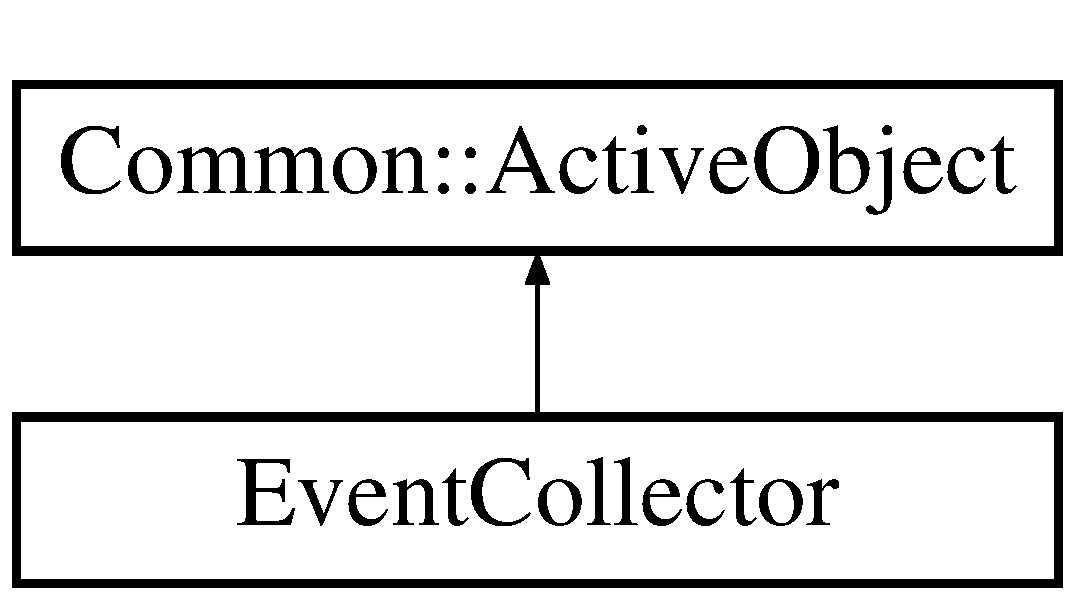
\includegraphics[height=2.000000cm]{class_event_collector}
\end{center}
\end{figure}
\subsection*{Public Types}
\begin{DoxyCompactItemize}
\item 
enum \{ {\bfseries Default\-Port}
 \}
\end{DoxyCompactItemize}
\subsection*{Public Member Functions}
\begin{DoxyCompactItemize}
\item 
\hyperlink{class_event_collector_a36de1ef281ba1c800a0b83ba18233f57}{Event\-Collector} (int port=Default\-Port)
\begin{DoxyCompactList}\small\item\em Constructor, starts an execution thread. \end{DoxyCompactList}\item 
\hypertarget{class_event_collector_a557c234313d714eb7a07b595a002b324}{\hyperlink{class_event_collector_a557c234313d714eb7a07b595a002b324}{$\sim$\-Event\-Collector} ()}\label{class_event_collector_a557c234313d714eb7a07b595a002b324}

\begin{DoxyCompactList}\small\item\em Destructor, stops the execution thread. \end{DoxyCompactList}\item 
void \hyperlink{class_event_collector_a42a1e721b13f06f5733aabd03804a165}{Set\-Listener} (\hyperlink{class_event_listener}{Event\-Listener} $\ast$listener)
\begin{DoxyCompactList}\small\item\em Setter for the listener. \end{DoxyCompactList}\item 
\hyperlink{class_event_listener}{Event\-Listener} $\ast$ \hyperlink{class_event_collector_a5897ca33a4baf5fb3cd2a32ec411af1f}{Get\-Listener} ()
\begin{DoxyCompactList}\small\item\em Getter for the listener. \end{DoxyCompactList}\item 
bool \hyperlink{class_event_collector_a6ca1544d70c43e753ee40bc60937e27e}{Is\-Aborted} () const 
\begin{DoxyCompactList}\small\item\em Determines if the collector is aborted. \end{DoxyCompactList}\end{DoxyCompactItemize}
\subsection*{Protected Member Functions}
\begin{DoxyCompactItemize}
\item 
\hypertarget{class_event_collector_a5856093a6f5813af9a8ff5b6d086d159}{void \hyperlink{class_event_collector_a5856093a6f5813af9a8ff5b6d086d159}{Init\-Thread} ()}\label{class_event_collector_a5856093a6f5813af9a8ff5b6d086d159}

\begin{DoxyCompactList}\small\item\em Not implemented (here for compatibility reasons). \end{DoxyCompactList}\item 
\hypertarget{class_event_collector_a5432f799527c116921834de45db7db52}{void \hyperlink{class_event_collector_a5432f799527c116921834de45db7db52}{Run} ()}\label{class_event_collector_a5432f799527c116921834de45db7db52}

\begin{DoxyCompactList}\small\item\em Runner of the execution thread, handles events until it dies. \end{DoxyCompactList}\item 
\hypertarget{class_event_collector_aae0e6be4959f8649e581dd4b1b58ed49}{void \hyperlink{class_event_collector_aae0e6be4959f8649e581dd4b1b58ed49}{Flush\-Thread} ()}\label{class_event_collector_aae0e6be4959f8649e581dd4b1b58ed49}

\begin{DoxyCompactList}\small\item\em Not implemented (here for compatibility reasons). \end{DoxyCompactList}\item 
\hypertarget{class_event_collector_af3ec06337a16aab00debe03334fe3955}{void \hyperlink{class_event_collector_af3ec06337a16aab00debe03334fe3955}{Fatal} ()}\label{class_event_collector_af3ec06337a16aab00debe03334fe3955}

\begin{DoxyCompactList}\small\item\em Called when an exception is caught in the execution thread. \end{DoxyCompactList}\end{DoxyCompactItemize}
\subsection*{Protected Attributes}
\begin{DoxyCompactItemize}
\item 
\hypertarget{class_event_collector_a804a727da52b6e87b2d0a4085b65f69a}{\hyperlink{class_event_listener}{Event\-Listener} $\ast$ {\bfseries \-\_\-listener}}\label{class_event_collector_a804a727da52b6e87b2d0a4085b65f69a}

\item 
\hypertarget{class_event_collector_a98a09cb97be226f2886c392fdd4e0d03}{\hyperlink{class_common_1_1_reactor}{Reactor} {\bfseries \-\_\-reactor}}\label{class_event_collector_a98a09cb97be226f2886c392fdd4e0d03}

\item 
\hypertarget{class_event_collector_a613769c93fe837bb12605ad07dae43e8}{\hyperlink{class_e_c_p_acceptor}{E\-C\-P\-Acceptor} {\bfseries \-\_\-acceptor}}\label{class_event_collector_a613769c93fe837bb12605ad07dae43e8}

\item 
\hypertarget{class_event_collector_aae721554b784e9565bfc889396726881}{bool {\bfseries \-\_\-aborted}}\label{class_event_collector_aae721554b784e9565bfc889396726881}

\end{DoxyCompactItemize}


\subsection{Detailed Description}
Processes the incoming event records from the D\-M\-Libs. It is based on an active object (thread) that collects incoming E\-C\-P events It stores a moving window of events incoming from different processes using a pool of buffers. The maximum size of this event window can be configured by the tunlets. 

\subsection{Constructor \& Destructor Documentation}
\hypertarget{class_event_collector_a36de1ef281ba1c800a0b83ba18233f57}{\index{Event\-Collector@{Event\-Collector}!Event\-Collector@{Event\-Collector}}
\index{Event\-Collector@{Event\-Collector}!EventCollector@{Event\-Collector}}
\subsubsection[{Event\-Collector}]{\setlength{\rightskip}{0pt plus 5cm}Event\-Collector\-::\-Event\-Collector (
\begin{DoxyParamCaption}
\item[{int}]{port = {\ttfamily DefaultPort}}
\end{DoxyParamCaption}
)}}\label{class_event_collector_a36de1ef281ba1c800a0b83ba18233f57}


Constructor, starts an execution thread. 


\begin{DoxyParams}{Parameters}
{\em port} & Acceptor port. \\
\hline
\end{DoxyParams}


\subsection{Member Function Documentation}
\hypertarget{class_event_collector_a5897ca33a4baf5fb3cd2a32ec411af1f}{\index{Event\-Collector@{Event\-Collector}!Get\-Listener@{Get\-Listener}}
\index{Get\-Listener@{Get\-Listener}!EventCollector@{Event\-Collector}}
\subsubsection[{Get\-Listener}]{\setlength{\rightskip}{0pt plus 5cm}{\bf Event\-Listener}$\ast$ Event\-Collector\-::\-Get\-Listener (
\begin{DoxyParamCaption}
{}
\end{DoxyParamCaption}
)\hspace{0.3cm}{\ttfamily [inline]}}}\label{class_event_collector_a5897ca33a4baf5fb3cd2a32ec411af1f}


Getter for the listener. 

\begin{DoxyReturn}{Returns}
Listener of the event collector. 
\end{DoxyReturn}
\hypertarget{class_event_collector_a6ca1544d70c43e753ee40bc60937e27e}{\index{Event\-Collector@{Event\-Collector}!Is\-Aborted@{Is\-Aborted}}
\index{Is\-Aborted@{Is\-Aborted}!EventCollector@{Event\-Collector}}
\subsubsection[{Is\-Aborted}]{\setlength{\rightskip}{0pt plus 5cm}bool Event\-Collector\-::\-Is\-Aborted (
\begin{DoxyParamCaption}
{}
\end{DoxyParamCaption}
) const\hspace{0.3cm}{\ttfamily [inline]}}}\label{class_event_collector_a6ca1544d70c43e753ee40bc60937e27e}


Determines if the collector is aborted. 

\begin{DoxyReturn}{Returns}
The status of the collector. 
\end{DoxyReturn}
\hypertarget{class_event_collector_a42a1e721b13f06f5733aabd03804a165}{\index{Event\-Collector@{Event\-Collector}!Set\-Listener@{Set\-Listener}}
\index{Set\-Listener@{Set\-Listener}!EventCollector@{Event\-Collector}}
\subsubsection[{Set\-Listener}]{\setlength{\rightskip}{0pt plus 5cm}void Event\-Collector\-::\-Set\-Listener (
\begin{DoxyParamCaption}
\item[{{\bf Event\-Listener} $\ast$}]{listener}
\end{DoxyParamCaption}
)}}\label{class_event_collector_a42a1e721b13f06f5733aabd03804a165}


Setter for the listener. 


\begin{DoxyParams}{Parameters}
{\em listener} & Listener to be set. \\
\hline
\end{DoxyParams}


The documentation for this class was generated from the following files\-:\begin{DoxyCompactItemize}
\item 
Analyzer/Event\-Collector.\-h\item 
Analyzer/Event\-Collector.\-cpp\end{DoxyCompactItemize}

\hypertarget{class_d_m_lib_1_1_event_collector_proxy}{\section{D\-M\-Lib\-:\-:Event\-Collector\-Proxy Class Reference}
\label{class_d_m_lib_1_1_event_collector_proxy}\index{D\-M\-Lib\-::\-Event\-Collector\-Proxy@{D\-M\-Lib\-::\-Event\-Collector\-Proxy}}
}


Connects to the analyzer host and sends requests.  




{\ttfamily \#include $<$E\-C\-P\-Proxy.\-h$>$}

\subsection*{Public Member Functions}
\begin{DoxyCompactItemize}
\item 
\hypertarget{class_d_m_lib_1_1_event_collector_proxy_a363b2b90626f1d08102b6628a65b61a1}{\hyperlink{class_d_m_lib_1_1_event_collector_proxy_a363b2b90626f1d08102b6628a65b61a1}{Event\-Collector\-Proxy} (std\-::string const \&host, int port)}\label{class_d_m_lib_1_1_event_collector_proxy_a363b2b90626f1d08102b6628a65b61a1}

\begin{DoxyCompactList}\small\item\em Constructor. \end{DoxyCompactList}\item 
\hypertarget{class_d_m_lib_1_1_event_collector_proxy_a6a43500ceae0fc7bcf3bf958e1e0689b}{\hyperlink{class_d_m_lib_1_1_event_collector_proxy_a6a43500ceae0fc7bcf3bf958e1e0689b}{$\sim$\-Event\-Collector\-Proxy} ()}\label{class_d_m_lib_1_1_event_collector_proxy_a6a43500ceae0fc7bcf3bf958e1e0689b}

\begin{DoxyCompactList}\small\item\em Destructor. \end{DoxyCompactList}\item 
\hypertarget{class_d_m_lib_1_1_event_collector_proxy_a2e030001e9d2649f020f02455aa5ebea}{void \hyperlink{class_d_m_lib_1_1_event_collector_proxy_a2e030001e9d2649f020f02455aa5ebea}{Register\-Lib} (int pid, int mpi\-Rank, std\-::string host, std\-::string task\-Name, int A\-Cport)}\label{class_d_m_lib_1_1_event_collector_proxy_a2e030001e9d2649f020f02455aa5ebea}

\begin{DoxyCompactList}\small\item\em Sends a request to the \hyperlink{class_analyzer}{Analyzer} to register a new worker. \end{DoxyCompactList}\item 
\hypertarget{class_d_m_lib_1_1_event_collector_proxy_a3c35713deece278377a1f265af7e1371}{void \hyperlink{class_d_m_lib_1_1_event_collector_proxy_a3c35713deece278377a1f265af7e1371}{Send\-Event} (\hyperlink{class_common_1_1_event_msg}{Event\-Msg} const \&event)}\label{class_d_m_lib_1_1_event_collector_proxy_a3c35713deece278377a1f265af7e1371}

\begin{DoxyCompactList}\small\item\em Sends a message to the analyzer. \end{DoxyCompactList}\item 
\hypertarget{class_d_m_lib_1_1_event_collector_proxy_ab65910277b0b1a35011f0a8b945417f0}{void \hyperlink{class_d_m_lib_1_1_event_collector_proxy_ab65910277b0b1a35011f0a8b945417f0}{Unregister\-Library} (int pid)}\label{class_d_m_lib_1_1_event_collector_proxy_ab65910277b0b1a35011f0a8b945417f0}

\begin{DoxyCompactList}\small\item\em Sends a request to the \hyperlink{class_analyzer}{Analyzer} to unregister a worker. \end{DoxyCompactList}\end{DoxyCompactItemize}


\subsection{Detailed Description}
Connects to the analyzer host and sends requests. 

\begin{DoxyVersion}{Version}
1.\-0b 
\end{DoxyVersion}
\begin{DoxySince}{Since}
1.\-0b 
\end{DoxySince}
\begin{DoxyAuthor}{Author}
Ania Sikora, 2002 
\end{DoxyAuthor}


The documentation for this class was generated from the following files\-:\begin{DoxyCompactItemize}
\item 
D\-M\-Lib/E\-C\-P\-Proxy.\-h\item 
D\-M\-Lib/E\-C\-P\-Proxy.\-cpp\end{DoxyCompactItemize}

\hypertarget{class_common_1_1_event_demultiplexer}{\section{Common\-:\-:Event\-Demultiplexer Class Reference}
\label{class_common_1_1_event_demultiplexer}\index{Common\-::\-Event\-Demultiplexer@{Common\-::\-Event\-Demultiplexer}}
}


Part of the reactor design pattern, takes requests coming from the reactor and passes them to different handlers.  




{\ttfamily \#include $<$Reactor.\-h$>$}

\subsection*{Public Member Functions}
\begin{DoxyCompactItemize}
\item 
\hypertarget{class_common_1_1_event_demultiplexer_a1049691d966410037859a9f4375fa613}{\hyperlink{class_common_1_1_event_demultiplexer_a1049691d966410037859a9f4375fa613}{Event\-Demultiplexer} ()}\label{class_common_1_1_event_demultiplexer_a1049691d966410037859a9f4375fa613}

\begin{DoxyCompactList}\small\item\em Constructor. \end{DoxyCompactList}\item 
\hypertarget{class_common_1_1_event_demultiplexer_a23812d729f572fd906678cec99f3a2b8}{void \hyperlink{class_common_1_1_event_demultiplexer_a23812d729f572fd906678cec99f3a2b8}{Add\-Handle} (int handle)}\label{class_common_1_1_event_demultiplexer_a23812d729f572fd906678cec99f3a2b8}

\begin{DoxyCompactList}\small\item\em Adds a new handle. \end{DoxyCompactList}\item 
\hypertarget{class_common_1_1_event_demultiplexer_a87eafa05d0a9d188bdc2b1548a656f6b}{void \hyperlink{class_common_1_1_event_demultiplexer_a87eafa05d0a9d188bdc2b1548a656f6b}{Remove\-Handle} (int handle)}\label{class_common_1_1_event_demultiplexer_a87eafa05d0a9d188bdc2b1548a656f6b}

\begin{DoxyCompactList}\small\item\em Removes selected handle. \end{DoxyCompactList}\item 
int \hyperlink{class_common_1_1_event_demultiplexer_a3174a4e1ce07e6ec8875fa8a1dd59379}{Select} (\hyperlink{class_common_1_1_time_value}{Time\-Value} $\ast$timeout=0)
\begin{DoxyCompactList}\small\item\em Returns the number of socket handles ready or 0 if the time limit expired. \end{DoxyCompactList}\item 
\hypertarget{class_common_1_1_event_demultiplexer_a4e4f26eb5cc25fe11ec2a3da90d732f0}{bool \hyperlink{class_common_1_1_event_demultiplexer_a4e4f26eb5cc25fe11ec2a3da90d732f0}{Is\-Handle\-Activated} (int handle) const }\label{class_common_1_1_event_demultiplexer_a4e4f26eb5cc25fe11ec2a3da90d732f0}

\begin{DoxyCompactList}\small\item\em Returns true if the given handle is activated, false otherwise. \end{DoxyCompactList}\item 
\hypertarget{class_common_1_1_event_demultiplexer_a5555e8ce92aae4bd661d0283525252ac}{int \hyperlink{class_common_1_1_event_demultiplexer_a5555e8ce92aae4bd661d0283525252ac}{Get\-Max\-Handle} () const }\label{class_common_1_1_event_demultiplexer_a5555e8ce92aae4bd661d0283525252ac}

\begin{DoxyCompactList}\small\item\em Returns value of the max handle. \end{DoxyCompactList}\end{DoxyCompactItemize}


\subsection{Detailed Description}
Part of the reactor design pattern, takes requests coming from the reactor and passes them to different handlers. 

\begin{DoxyVersion}{Version}
1.\-0 
\end{DoxyVersion}
\begin{DoxySince}{Since}
1.\-0 
\end{DoxySince}
\begin{DoxyAuthor}{Author}
Ania Sikora, 2002 
\end{DoxyAuthor}


\subsection{Member Function Documentation}
\hypertarget{class_common_1_1_event_demultiplexer_a3174a4e1ce07e6ec8875fa8a1dd59379}{\index{Common\-::\-Event\-Demultiplexer@{Common\-::\-Event\-Demultiplexer}!Select@{Select}}
\index{Select@{Select}!Common::EventDemultiplexer@{Common\-::\-Event\-Demultiplexer}}
\subsubsection[{Select}]{\setlength{\rightskip}{0pt plus 5cm}int Event\-Demultiplexer\-::\-Select (
\begin{DoxyParamCaption}
\item[{{\bf Time\-Value} $\ast$}]{timeout = {\ttfamily 0}}
\end{DoxyParamCaption}
)}}\label{class_common_1_1_event_demultiplexer_a3174a4e1ce07e6ec8875fa8a1dd59379}


Returns the number of socket handles ready or 0 if the time limit expired. 


\begin{DoxyParams}{Parameters}
{\em timeout} & If the parameter is a \hyperlink{class_common_1_1_time_value}{Time\-Value} object, it will wait the object value for events. In the event that the value is 0 it will check without blocking. If the parameter is a 0 (not a \hyperlink{class_common_1_1_time_value}{Time\-Value} object, default value) it will check and block in a forever loop. \\
\hline
\end{DoxyParams}


The documentation for this class was generated from the following files\-:\begin{DoxyCompactItemize}
\item 
Common/Reactor.\-h\item 
Common/Reactor.\-cpp\end{DoxyCompactItemize}

\hypertarget{class_common_1_1_event_exception}{\section{Common\-:\-:Event\-Exception Class Reference}
\label{class_common_1_1_event_exception}\index{Common\-::\-Event\-Exception@{Common\-::\-Event\-Exception}}
}


\hyperlink{class_common_1_1_event}{Event}, \hyperlink{class_common_1_1_event_map}{Event\-Map} and \hyperlink{class_common_1_1_event_handler}{Event\-Handler} exceptions.  




{\ttfamily \#include $<$Event\-Exception.\-h$>$}

Inheritance diagram for Common\-:\-:Event\-Exception\-:\begin{figure}[H]
\begin{center}
\leavevmode
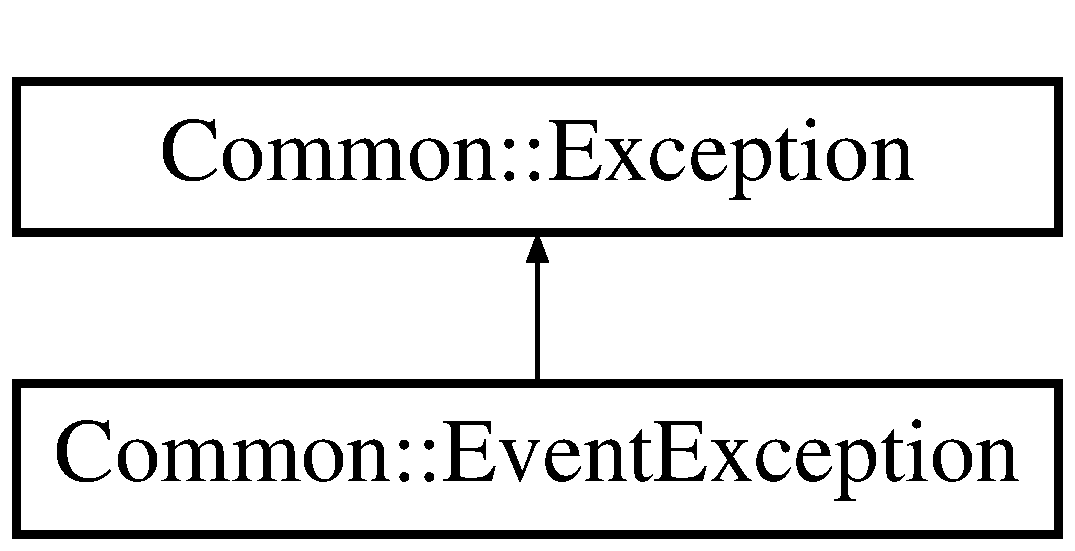
\includegraphics[height=2.000000cm]{class_common_1_1_event_exception}
\end{center}
\end{figure}
\subsection*{Public Member Functions}
\begin{DoxyCompactItemize}
\item 
\hyperlink{class_common_1_1_event_exception_ade643b92ec36ce7a991aa832f54e9a2e}{Event\-Exception} (std\-::string const \&msg, std\-::string const \&obj\-Name=std\-::string())
\begin{DoxyCompactList}\small\item\em Constructor. \end{DoxyCompactList}\item 
void \hyperlink{class_common_1_1_event_exception_a9f09705ed5302e3f1c0b000e10b7292a}{Display} (std\-::ostream \&os) const 
\begin{DoxyCompactList}\small\item\em Displays exception message on the given output stream. \end{DoxyCompactList}\item 
\hypertarget{class_common_1_1_event_exception_a0f43e1355f256c8158c742af79d1195d}{void \hyperlink{class_common_1_1_event_exception_a0f43e1355f256c8158c742af79d1195d}{Display} () const }\label{class_common_1_1_event_exception_a0f43e1355f256c8158c742af79d1195d}

\begin{DoxyCompactList}\small\item\em Displays exception message on the standard error output. \end{DoxyCompactList}\item 
std\-::string \hyperlink{class_common_1_1_event_exception_a979706b5799fd0e3fd128a36f34ab8cb}{Get\-Reason} () const 
\begin{DoxyCompactList}\small\item\em Returns a string containing the error message. \end{DoxyCompactList}\end{DoxyCompactItemize}
\subsection*{Additional Inherited Members}


\subsection{Detailed Description}
\hyperlink{class_common_1_1_event}{Event}, \hyperlink{class_common_1_1_event_map}{Event\-Map} and \hyperlink{class_common_1_1_event_handler}{Event\-Handler} exceptions. 

\begin{DoxyVersion}{Version}
1.\-0b 
\end{DoxyVersion}
\begin{DoxySince}{Since}
1.\-0b 
\end{DoxySince}
\begin{DoxyAuthor}{Author}
Noel De Martin, 2011 
\end{DoxyAuthor}


\subsection{Constructor \& Destructor Documentation}
\hypertarget{class_common_1_1_event_exception_ade643b92ec36ce7a991aa832f54e9a2e}{\index{Common\-::\-Event\-Exception@{Common\-::\-Event\-Exception}!Event\-Exception@{Event\-Exception}}
\index{Event\-Exception@{Event\-Exception}!Common::EventException@{Common\-::\-Event\-Exception}}
\subsubsection[{Event\-Exception}]{\setlength{\rightskip}{0pt plus 5cm}Common\-::\-Event\-Exception\-::\-Event\-Exception (
\begin{DoxyParamCaption}
\item[{std\-::string const \&}]{msg, }
\item[{std\-::string const \&}]{obj\-Name = {\ttfamily std\-:\-:string~()}}
\end{DoxyParamCaption}
)\hspace{0.3cm}{\ttfamily [inline]}}}\label{class_common_1_1_event_exception_ade643b92ec36ce7a991aa832f54e9a2e}


Constructor. 


\begin{DoxyParams}{Parameters}
{\em msg} & \hyperlink{class_common_1_1_exception}{Exception} message. \\
\hline
{\em obj\-Name} & Name of the object causing the exception, \char`\"{}\char`\"{} by default. \\
\hline
\end{DoxyParams}


\subsection{Member Function Documentation}
\hypertarget{class_common_1_1_event_exception_a9f09705ed5302e3f1c0b000e10b7292a}{\index{Common\-::\-Event\-Exception@{Common\-::\-Event\-Exception}!Display@{Display}}
\index{Display@{Display}!Common::EventException@{Common\-::\-Event\-Exception}}
\subsubsection[{Display}]{\setlength{\rightskip}{0pt plus 5cm}void Common\-::\-Event\-Exception\-::\-Display (
\begin{DoxyParamCaption}
\item[{std\-::ostream \&}]{os}
\end{DoxyParamCaption}
) const\hspace{0.3cm}{\ttfamily [virtual]}}}\label{class_common_1_1_event_exception_a9f09705ed5302e3f1c0b000e10b7292a}


Displays exception message on the given output stream. 


\begin{DoxyParams}{Parameters}
{\em os} & Output stream to display the message. \\
\hline
\end{DoxyParams}


Reimplemented from \hyperlink{class_common_1_1_exception_a2633eeaab3220268739977a04643a3cf}{Common\-::\-Exception}.

\hypertarget{class_common_1_1_event_exception_a979706b5799fd0e3fd128a36f34ab8cb}{\index{Common\-::\-Event\-Exception@{Common\-::\-Event\-Exception}!Get\-Reason@{Get\-Reason}}
\index{Get\-Reason@{Get\-Reason}!Common::EventException@{Common\-::\-Event\-Exception}}
\subsubsection[{Get\-Reason}]{\setlength{\rightskip}{0pt plus 5cm}string Event\-Exception\-::\-Get\-Reason (
\begin{DoxyParamCaption}
{}
\end{DoxyParamCaption}
) const}}\label{class_common_1_1_event_exception_a979706b5799fd0e3fd128a36f34ab8cb}


Returns a string containing the error message. 

\begin{DoxyReturn}{Returns}
String with the error. 
\end{DoxyReturn}


The documentation for this class was generated from the following files\-:\begin{DoxyCompactItemize}
\item 
Common/Event\-Exception.\-h\item 
Common/Event\-Exception.\-cpp\end{DoxyCompactItemize}

\hypertarget{class_common_1_1_event_handler}{\section{Common\-:\-:Event\-Handler Class Reference}
\label{class_common_1_1_event_handler}\index{Common\-::\-Event\-Handler@{Common\-::\-Event\-Handler}}
}


Abstract class, processes the requests sent to the reactor.  




{\ttfamily \#include $<$Event\-Handler.\-h$>$}

Inheritance diagram for Common\-:\-:Event\-Handler\-:\begin{figure}[H]
\begin{center}
\leavevmode
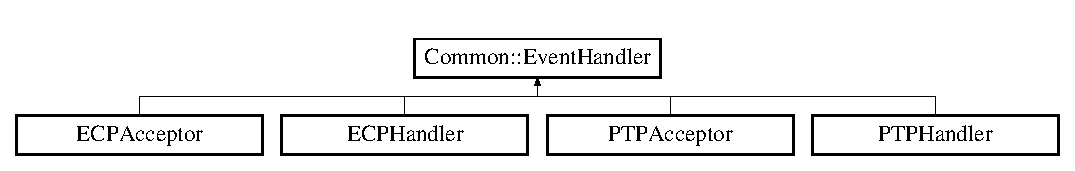
\includegraphics[height=1.854305cm]{class_common_1_1_event_handler}
\end{center}
\end{figure}
\subsection*{Public Member Functions}
\begin{DoxyCompactItemize}
\item 
\hypertarget{class_common_1_1_event_handler_a82426b7867c0a2fda62ab4c159cd24be}{virtual void \hyperlink{class_common_1_1_event_handler_a82426b7867c0a2fda62ab4c159cd24be}{Handle\-Input} ()=0}\label{class_common_1_1_event_handler_a82426b7867c0a2fda62ab4c159cd24be}

\begin{DoxyCompactList}\small\item\em Reads the data from the socket and treats it. \end{DoxyCompactList}\item 
\hypertarget{class_common_1_1_event_handler_aaf6cb56038c6fe6b91c9d1e34ee6b3af}{virtual int \hyperlink{class_common_1_1_event_handler_aaf6cb56038c6fe6b91c9d1e34ee6b3af}{Get\-Handle} ()=0}\label{class_common_1_1_event_handler_aaf6cb56038c6fe6b91c9d1e34ee6b3af}

\begin{DoxyCompactList}\small\item\em Returns socket descriptor. \end{DoxyCompactList}\end{DoxyCompactItemize}


\subsection{Detailed Description}
Abstract class, processes the requests sent to the reactor. 

\begin{DoxyVersion}{Version}
1.\-0b 
\end{DoxyVersion}
\begin{DoxySince}{Since}
1.\-0b 
\end{DoxySince}
\begin{DoxyAuthor}{Author}
Ania Sikora, 2002 
\end{DoxyAuthor}


The documentation for this class was generated from the following file\-:\begin{DoxyCompactItemize}
\item 
Common/Event\-Handler.\-h\end{DoxyCompactItemize}

\hypertarget{class_model_1_1_event_handler}{\section{Model\-:\-:Event\-Handler Class Reference}
\label{class_model_1_1_event_handler}\index{Model\-::\-Event\-Handler@{Model\-::\-Event\-Handler}}
}


Abstract class that holds a method to manage event records.  




{\ttfamily \#include $<$App\-Event.\-h$>$}

Inheritance diagram for Model\-:\-:Event\-Handler\-:\begin{figure}[H]
\begin{center}
\leavevmode
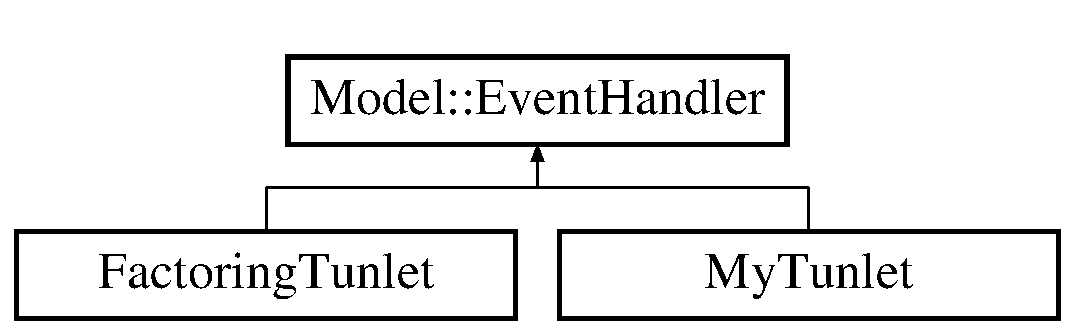
\includegraphics[height=2.000000cm]{class_model_1_1_event_handler}
\end{center}
\end{figure}
\subsection*{Public Member Functions}
\begin{DoxyCompactItemize}
\item 
virtual void \hyperlink{class_model_1_1_event_handler_a0a84c727f41c358350a2f3522ffba03b}{Handle\-Event} (\hyperlink{class_model_1_1_event_record}{Event\-Record} const \&r)=0
\begin{DoxyCompactList}\small\item\em Handles an event record (virtual). \end{DoxyCompactList}\end{DoxyCompactItemize}


\subsection{Detailed Description}
Abstract class that holds a method to manage event records. 

\subsection{Member Function Documentation}
\hypertarget{class_model_1_1_event_handler_a0a84c727f41c358350a2f3522ffba03b}{\index{Model\-::\-Event\-Handler@{Model\-::\-Event\-Handler}!Handle\-Event@{Handle\-Event}}
\index{Handle\-Event@{Handle\-Event}!Model::EventHandler@{Model\-::\-Event\-Handler}}
\subsubsection[{Handle\-Event}]{\setlength{\rightskip}{0pt plus 5cm}virtual void Model\-::\-Event\-Handler\-::\-Handle\-Event (
\begin{DoxyParamCaption}
\item[{{\bf Event\-Record} const \&}]{r}
\end{DoxyParamCaption}
)\hspace{0.3cm}{\ttfamily [pure virtual]}}}\label{class_model_1_1_event_handler_a0a84c727f41c358350a2f3522ffba03b}


Handles an event record (virtual). 


\begin{DoxyParams}{Parameters}
{\em r} & \hyperlink{class_model_1_1_event}{Event} record to be handled \\
\hline
\end{DoxyParams}


Implemented in \hyperlink{class_factoring_tunlet_aeb954297fd00f2801c807ef3ae2384f1}{Factoring\-Tunlet}, and \hyperlink{class_my_tunlet_af1b66922cbdce93415ef288ca36b3106}{My\-Tunlet}.



The documentation for this class was generated from the following file\-:\begin{DoxyCompactItemize}
\item 
Analyzer/App\-Event.\-h\end{DoxyCompactItemize}

\hypertarget{class_event_listener}{\section{Event\-Listener Class Reference}
\label{class_event_listener}\index{Event\-Listener@{Event\-Listener}}
}


Provides an interface for event listeners, which consist in methods to respond to events and errors.  




{\ttfamily \#include $<$Event\-Collector.\-h$>$}

Inheritance diagram for Event\-Listener\-:\begin{figure}[H]
\begin{center}
\leavevmode
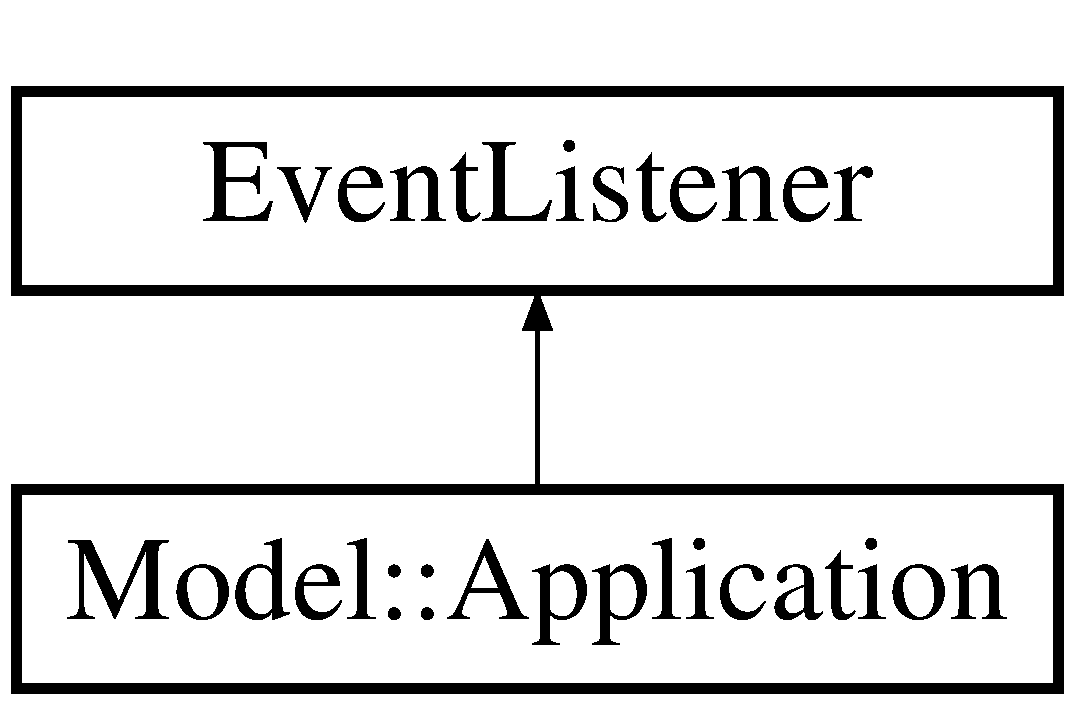
\includegraphics[height=2.000000cm]{class_event_listener}
\end{center}
\end{figure}
\subsection*{Public Member Functions}
\begin{DoxyCompactItemize}
\item 
virtual void \hyperlink{class_event_listener_a0e6f686e8d0abb100c3fbce37586b04b}{On\-Event} (\hyperlink{class_common_1_1_e_c_p_message}{E\-C\-P\-Message} $\ast$msg)=0
\begin{DoxyCompactList}\small\item\em Function which is triggered when an event happens. \end{DoxyCompactList}\item 
\hypertarget{class_event_listener_a77e58660b8b6910d36a961384032697e}{virtual void \hyperlink{class_event_listener_a77e58660b8b6910d36a961384032697e}{On\-Fatal\-Error} ()=0}\label{class_event_listener_a77e58660b8b6910d36a961384032697e}

\begin{DoxyCompactList}\small\item\em Function which is triggered when a fatal error happens. \end{DoxyCompactList}\end{DoxyCompactItemize}


\subsection{Detailed Description}
Provides an interface for event listeners, which consist in methods to respond to events and errors. 

\subsection{Member Function Documentation}
\hypertarget{class_event_listener_a0e6f686e8d0abb100c3fbce37586b04b}{\index{Event\-Listener@{Event\-Listener}!On\-Event@{On\-Event}}
\index{On\-Event@{On\-Event}!EventListener@{Event\-Listener}}
\subsubsection[{On\-Event}]{\setlength{\rightskip}{0pt plus 5cm}virtual void Event\-Listener\-::\-On\-Event (
\begin{DoxyParamCaption}
\item[{{\bf E\-C\-P\-Message} $\ast$}]{msg}
\end{DoxyParamCaption}
)\hspace{0.3cm}{\ttfamily [pure virtual]}}}\label{class_event_listener_a0e6f686e8d0abb100c3fbce37586b04b}


Function which is triggered when an event happens. 


\begin{DoxyParams}{Parameters}
{\em msg} & Message that contains the event data. \\
\hline
\end{DoxyParams}


Implemented in \hyperlink{class_model_1_1_application_aeb4e28cb6431a3b073dcf379731ec614}{Model\-::\-Application}.



The documentation for this class was generated from the following file\-:\begin{DoxyCompactItemize}
\item 
Analyzer/Event\-Collector.\-h\end{DoxyCompactItemize}

\hypertarget{class_common_1_1_event_map}{\section{Common\-:\-:Event\-Map Class Reference}
\label{class_common_1_1_event_map}\index{Common\-::\-Event\-Map@{Common\-::\-Event\-Map}}
}


Contains and manages a collection of \hyperlink{class_common_1_1_event}{Event} objects.  




{\ttfamily \#include $<$Event\-Map.\-h$>$}

\subsection*{Public Member Functions}
\begin{DoxyCompactItemize}
\item 
\hypertarget{class_common_1_1_event_map_a2ecd4953116dbcc2fa41cb3197154e05}{\hyperlink{class_common_1_1_event_map_a2ecd4953116dbcc2fa41cb3197154e05}{Event\-Map} ()}\label{class_common_1_1_event_map_a2ecd4953116dbcc2fa41cb3197154e05}

\begin{DoxyCompactList}\small\item\em Constructor. \end{DoxyCompactList}\item 
void \hyperlink{class_common_1_1_event_map_a4cc364f80ededaab7215e0de7df690a5}{Add} (std\-::string const \&name, int id)
\begin{DoxyCompactList}\small\item\em Adds a new event into the map. \end{DoxyCompactList}\item 
int \hyperlink{class_common_1_1_event_map_a3f3e9ec582e4cccdca6f12ac70d181f8}{Get\-Id} (std\-::string const \&name) const 
\begin{DoxyCompactList}\small\item\em Returns id of the given event. \end{DoxyCompactList}\item 
\hypertarget{class_common_1_1_event_map_a4de4e93e992b4beb406b164c23ed4ea9}{int \hyperlink{class_common_1_1_event_map_a4de4e93e992b4beb406b164c23ed4ea9}{Get\-Size} () const }\label{class_common_1_1_event_map_a4de4e93e992b4beb406b164c23ed4ea9}

\begin{DoxyCompactList}\small\item\em Returns map size. \end{DoxyCompactList}\end{DoxyCompactItemize}


\subsection{Detailed Description}
Contains and manages a collection of \hyperlink{class_common_1_1_event}{Event} objects. 

\begin{DoxyVersion}{Version}
1.\-0b 
\end{DoxyVersion}
\begin{DoxySince}{Since}
1.\-0b 
\end{DoxySince}
\begin{DoxyAuthor}{Author}
Ania Sikora, 2001 
\end{DoxyAuthor}


\subsection{Member Function Documentation}
\hypertarget{class_common_1_1_event_map_a4cc364f80ededaab7215e0de7df690a5}{\index{Common\-::\-Event\-Map@{Common\-::\-Event\-Map}!Add@{Add}}
\index{Add@{Add}!Common::EventMap@{Common\-::\-Event\-Map}}
\subsubsection[{Add}]{\setlength{\rightskip}{0pt plus 5cm}void Event\-Map\-::\-Add (
\begin{DoxyParamCaption}
\item[{std\-::string const \&}]{name, }
\item[{int}]{id}
\end{DoxyParamCaption}
)}}\label{class_common_1_1_event_map_a4cc364f80ededaab7215e0de7df690a5}


Adds a new event into the map. 


\begin{DoxyExceptions}{Exceptions}
{\em \hyperlink{class_common_1_1_event_exception}{Event\-Exception}} & \\
\hline
\end{DoxyExceptions}
\hypertarget{class_common_1_1_event_map_a3f3e9ec582e4cccdca6f12ac70d181f8}{\index{Common\-::\-Event\-Map@{Common\-::\-Event\-Map}!Get\-Id@{Get\-Id}}
\index{Get\-Id@{Get\-Id}!Common::EventMap@{Common\-::\-Event\-Map}}
\subsubsection[{Get\-Id}]{\setlength{\rightskip}{0pt plus 5cm}int Event\-Map\-::\-Get\-Id (
\begin{DoxyParamCaption}
\item[{std\-::string const \&}]{name}
\end{DoxyParamCaption}
) const}}\label{class_common_1_1_event_map_a3f3e9ec582e4cccdca6f12ac70d181f8}


Returns id of the given event. 


\begin{DoxyExceptions}{Exceptions}
{\em \hyperlink{class_common_1_1_event_exception}{Event\-Exception}} & \\
\hline
\end{DoxyExceptions}


The documentation for this class was generated from the following files\-:\begin{DoxyCompactItemize}
\item 
Common/Event\-Map.\-h\item 
Common/Event\-Map.\-cpp\end{DoxyCompactItemize}

\hypertarget{class_common_1_1_event_msg}{\section{Common\-:\-:Event\-Msg Class Reference}
\label{class_common_1_1_event_msg}\index{Common\-::\-Event\-Msg@{Common\-::\-Event\-Msg}}
}


Encapsulates a message generated by D\-M\-Lib to trace events.  




{\ttfamily \#include $<$E\-C\-P\-Msg.\-h$>$}

Inheritance diagram for Common\-:\-:Event\-Msg\-:\begin{figure}[H]
\begin{center}
\leavevmode
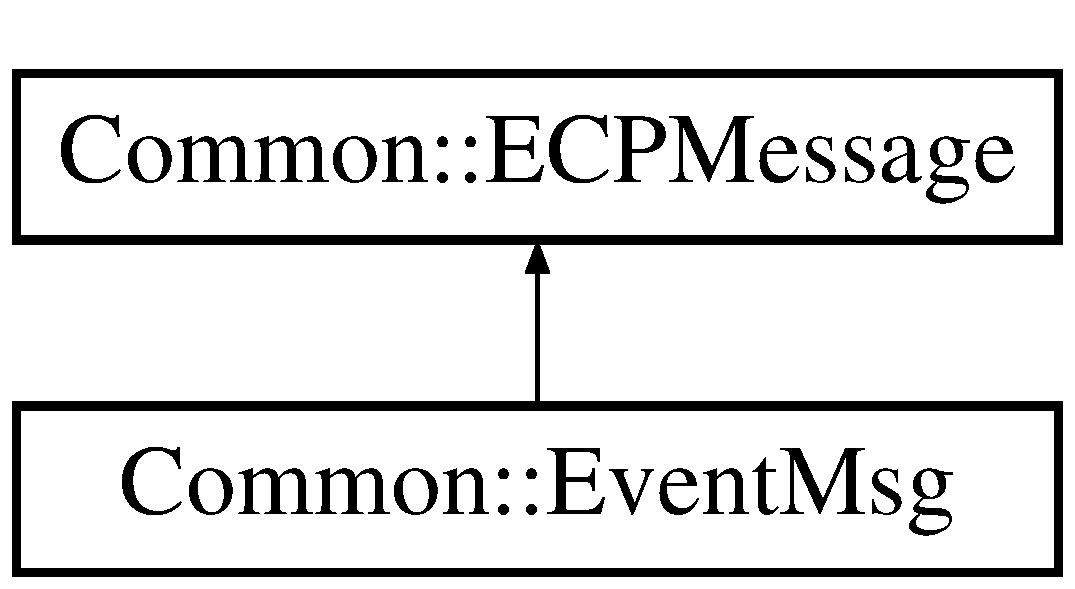
\includegraphics[height=2.000000cm]{class_common_1_1_event_msg}
\end{center}
\end{figure}
\subsection*{Public Member Functions}
\begin{DoxyCompactItemize}
\item 
\hypertarget{class_common_1_1_event_msg_a80cbc0730f7b70ae74babd298a91ec98}{\hyperlink{class_common_1_1_event_msg_a80cbc0730f7b70ae74babd298a91ec98}{Event\-Msg} ()}\label{class_common_1_1_event_msg_a80cbc0730f7b70ae74babd298a91ec98}

\begin{DoxyCompactList}\small\item\em Constructor. \end{DoxyCompactList}\item 
\hypertarget{class_common_1_1_event_msg_a74eb56c9e54447a26b7a646ba909531d}{\hyperlink{class_common_1_1_event_msg_a74eb56c9e54447a26b7a646ba909531d}{$\sim$\-Event\-Msg} ()}\label{class_common_1_1_event_msg_a74eb56c9e54447a26b7a646ba909531d}

\begin{DoxyCompactList}\small\item\em Destructor. \end{DoxyCompactList}\item 
void \hyperlink{class_common_1_1_event_msg_a3dfd468f489cfb9b3ca47a6ff7c31b66}{Reset} (long\-\_\-t timestamp, int event\-Id, Instr\-Place place, int param\-Count)
\begin{DoxyCompactList}\small\item\em Sets the message to the indicated state. \end{DoxyCompactList}\item 
\hypertarget{class_common_1_1_event_msg_a3214ec6fb7cb75e537484e16f626122f}{void \hyperlink{class_common_1_1_event_msg_a3214ec6fb7cb75e537484e16f626122f}{Set\-Tid} (int tid)}\label{class_common_1_1_event_msg_a3214ec6fb7cb75e537484e16f626122f}

\begin{DoxyCompactList}\small\item\em Sets the task id. \end{DoxyCompactList}\item 
\hypertarget{class_common_1_1_event_msg_a653dc46368270cfdc04f08330fabb8b0}{E\-C\-P\-Msg\-Type \hyperlink{class_common_1_1_event_msg_a653dc46368270cfdc04f08330fabb8b0}{Get\-Type} () const }\label{class_common_1_1_event_msg_a653dc46368270cfdc04f08330fabb8b0}

\begin{DoxyCompactList}\small\item\em Returns the type of event. \end{DoxyCompactList}\item 
\hypertarget{class_common_1_1_event_msg_a1f7e1bd0f49f01f90dde8aebfe34ead1}{void \hyperlink{class_common_1_1_event_msg_a1f7e1bd0f49f01f90dde8aebfe34ead1}{Set\-Params} (char const $\ast$buffer, int size)}\label{class_common_1_1_event_msg_a1f7e1bd0f49f01f90dde8aebfe34ead1}

\begin{DoxyCompactList}\small\item\em Sets the buffer to be used and indicates its size. \end{DoxyCompactList}\item 
\hypertarget{class_common_1_1_event_msg_a9c83946dd9eed41575874d9ceb0158f0}{void \hyperlink{class_common_1_1_event_msg_a9c83946dd9eed41575874d9ceb0158f0}{Set\-Buffer} (char $\ast$buffer)}\label{class_common_1_1_event_msg_a9c83946dd9eed41575874d9ceb0158f0}

\begin{DoxyCompactList}\small\item\em Sets the parameters buffer. \end{DoxyCompactList}\item 
\hypertarget{class_common_1_1_event_msg_af4a449ef5a8255be4d521bc75841727f}{int \hyperlink{class_common_1_1_event_msg_af4a449ef5a8255be4d521bc75841727f}{Get\-Param\-Buf\-Size} () const }\label{class_common_1_1_event_msg_af4a449ef5a8255be4d521bc75841727f}

\begin{DoxyCompactList}\small\item\em Returns buffer size. \end{DoxyCompactList}\item 
\hypertarget{class_common_1_1_event_msg_ab5a78181901292a807b71667bc500658}{const char $\ast$ \hyperlink{class_common_1_1_event_msg_ab5a78181901292a807b71667bc500658}{Get\-Param\-Buffer} () const }\label{class_common_1_1_event_msg_ab5a78181901292a807b71667bc500658}

\begin{DoxyCompactList}\small\item\em Returns a pointer to the content of the buffer. \end{DoxyCompactList}\item 
\hypertarget{class_common_1_1_event_msg_a208dcc28a9fca5e58bde25ef86e0399b}{long\-\_\-t \hyperlink{class_common_1_1_event_msg_a208dcc28a9fca5e58bde25ef86e0399b}{Get\-Timestamp} () const }\label{class_common_1_1_event_msg_a208dcc28a9fca5e58bde25ef86e0399b}

\begin{DoxyCompactList}\small\item\em Returns timestamp. \end{DoxyCompactList}\item 
\hypertarget{class_common_1_1_event_msg_ae0a26efc9d53bacf315e5950b15fb998}{int \hyperlink{class_common_1_1_event_msg_ae0a26efc9d53bacf315e5950b15fb998}{Get\-Place} () const }\label{class_common_1_1_event_msg_ae0a26efc9d53bacf315e5950b15fb998}

\begin{DoxyCompactList}\small\item\em Returns place where the event is located \{instr\-Unknown, ip\-Func\-Entry, ip\-Func\-Exit\}. \end{DoxyCompactList}\item 
\hypertarget{class_common_1_1_event_msg_ac3fdaca51c498c7ee4a91eafc62e0de1}{int \hyperlink{class_common_1_1_event_msg_ac3fdaca51c498c7ee4a91eafc62e0de1}{Get\-Event\-Id} () const }\label{class_common_1_1_event_msg_ac3fdaca51c498c7ee4a91eafc62e0de1}

\begin{DoxyCompactList}\small\item\em Returns event I\-D. \end{DoxyCompactList}\item 
\hypertarget{class_common_1_1_event_msg_a3f36752848f7fb4666f4e7fb6c0693ec}{int \hyperlink{class_common_1_1_event_msg_a3f36752848f7fb4666f4e7fb6c0693ec}{Get\-Param\-Count} () const }\label{class_common_1_1_event_msg_a3f36752848f7fb4666f4e7fb6c0693ec}

\begin{DoxyCompactList}\small\item\em Returns parameters count. \end{DoxyCompactList}\item 
\hypertarget{class_common_1_1_event_msg_af19391509b10c816e1051110c1c0b3d2}{int \hyperlink{class_common_1_1_event_msg_af19391509b10c816e1051110c1c0b3d2}{Get\-Data\-Size} () const }\label{class_common_1_1_event_msg_af19391509b10c816e1051110c1c0b3d2}

\begin{DoxyCompactList}\small\item\em Returns size of the data serialized. \end{DoxyCompactList}\item 
\hypertarget{class_common_1_1_event_msg_a2923792625324b618fd108f19664f444}{void \hyperlink{class_common_1_1_event_msg_a2923792625324b618fd108f19664f444}{Serialize} (\hyperlink{class_common_1_1_serializer}{Serializer} \&out) const }\label{class_common_1_1_event_msg_a2923792625324b618fd108f19664f444}

\begin{DoxyCompactList}\small\item\em Serializes the message with the given \hyperlink{class_common_1_1_serializer}{Serializer}. \end{DoxyCompactList}\item 
\hypertarget{class_common_1_1_event_msg_a404a3fa9bf89678d21551471e29e557b}{void \hyperlink{class_common_1_1_event_msg_a404a3fa9bf89678d21551471e29e557b}{De\-Serialize} (\hyperlink{class_common_1_1_de_serializer}{De\-Serializer} \&in)}\label{class_common_1_1_event_msg_a404a3fa9bf89678d21551471e29e557b}

\begin{DoxyCompactList}\small\item\em Deserializes the message with the given \hyperlink{class_common_1_1_de_serializer}{De\-Serializer}. \end{DoxyCompactList}\item 
\hypertarget{class_common_1_1_event_msg_a1046ace3b69874913fcdcda30471f3bd}{int \hyperlink{class_common_1_1_event_msg_a1046ace3b69874913fcdcda30471f3bd}{Get\-Tid} () const }\label{class_common_1_1_event_msg_a1046ace3b69874913fcdcda30471f3bd}

\begin{DoxyCompactList}\small\item\em Returns the task id. \end{DoxyCompactList}\end{DoxyCompactItemize}
\subsection*{Additional Inherited Members}


\subsection{Detailed Description}
Encapsulates a message generated by D\-M\-Lib to trace events. 

The message indicates what information should be gathered of certain event, this messages are created with an Event\-Msg\-Writer object.

\begin{DoxyVersion}{Version}
1.\-0b 
\end{DoxyVersion}
\begin{DoxySince}{Since}
1.\-0b 
\end{DoxySince}
\begin{DoxyAuthor}{Author}
Ania Sikora, 2002 
\end{DoxyAuthor}


\subsection{Member Function Documentation}
\hypertarget{class_common_1_1_event_msg_a3dfd468f489cfb9b3ca47a6ff7c31b66}{\index{Common\-::\-Event\-Msg@{Common\-::\-Event\-Msg}!Reset@{Reset}}
\index{Reset@{Reset}!Common::EventMsg@{Common\-::\-Event\-Msg}}
\subsubsection[{Reset}]{\setlength{\rightskip}{0pt plus 5cm}void Event\-Msg\-::\-Reset (
\begin{DoxyParamCaption}
\item[{long\-\_\-t}]{timestamp, }
\item[{int}]{event\-Id, }
\item[{Instr\-Place}]{place, }
\item[{int}]{param\-Count}
\end{DoxyParamCaption}
)}}\label{class_common_1_1_event_msg_a3dfd468f489cfb9b3ca47a6ff7c31b66}


Sets the message to the indicated state. 


\begin{DoxyParams}{Parameters}
{\em timestamp} & Timestamp when the event occurs. \\
\hline
{\em event\-Id} & Id of the event. \\
\hline
{\em place} & Place where the event is located \{instr\-Unknown, ip\-Func\-Entry, ip\-Func\-Exit\}. \\
\hline
{\em param\-Count} & Number of parameters. \\
\hline
\end{DoxyParams}


The documentation for this class was generated from the following files\-:\begin{DoxyCompactItemize}
\item 
Common/E\-C\-P\-Msg.\-h\item 
Common/E\-C\-P\-Msg.\-cpp\end{DoxyCompactItemize}

\hypertarget{class_event_msg_reader}{\section{Event\-Msg\-Reader Class Reference}
\label{class_event_msg_reader}\index{Event\-Msg\-Reader@{Event\-Msg\-Reader}}
}


Provides methods for getting data from event messages. The data structure that supports the class consist in the message to be processed, a buffer to hold the data and a deserializer object to reconstruct the information.  




{\ttfamily \#include $<$Event\-Msg\-Reader.\-h$>$}

\subsection*{Public Member Functions}
\begin{DoxyCompactItemize}
\item 
\hyperlink{class_event_msg_reader_adb478ebe048cf85cc6ea1fe7c1d900b4}{Event\-Msg\-Reader} (\hyperlink{class_common_1_1_event_msg}{Event\-Msg} const \&msg)
\begin{DoxyCompactList}\small\item\em Constructor. \end{DoxyCompactList}\item 
int \hyperlink{class_event_msg_reader_a87725095415b9cbc0938276423ab6ba2}{Get\-Param\-Count} () const 
\begin{DoxyCompactList}\small\item\em Getter of Param\-Count. \end{DoxyCompactList}\item 
Attr\-Value\-Type \hyperlink{class_event_msg_reader_a31d020728a4d984fd0e2d349f458d39a}{Get\-Attr\-Type} ()
\begin{DoxyCompactList}\small\item\em getter of Attr\-Type. \end{DoxyCompactList}\item 
int \hyperlink{class_event_msg_reader_a49dff56a337d6cd638e3df29064f12e0}{Get\-Int\-Value} ()
\begin{DoxyCompactList}\small\item\em Gets an integer from the stream. \end{DoxyCompactList}\item 
float \hyperlink{class_event_msg_reader_abba88cdac5d454e5684d320932155c0e}{Get\-Float\-Value} ()
\begin{DoxyCompactList}\small\item\em Gets a float from the stream. \end{DoxyCompactList}\item 
double \hyperlink{class_event_msg_reader_a151372639142577ffb57d99404babd5b}{Get\-Double\-Value} ()
\begin{DoxyCompactList}\small\item\em Gets a double from the stream. \end{DoxyCompactList}\item 
char \hyperlink{class_event_msg_reader_a2c7ff71a65e8f3e6140473df556874ea}{Get\-Char\-Value} ()
\begin{DoxyCompactList}\small\item\em Gets a character from the stream. \end{DoxyCompactList}\item 
short \hyperlink{class_event_msg_reader_af97d34d4b5c94a5bb7f1b88e9c285b8a}{Get\-Short\-Value} ()
\begin{DoxyCompactList}\small\item\em Gets a short from the stream. \end{DoxyCompactList}\item 
std\-::string \hyperlink{class_event_msg_reader_a0f641dc44b5bd73d3ce14a9421248a88}{Get\-String\-Value} ()
\begin{DoxyCompactList}\small\item\em Get a string from the stream. \end{DoxyCompactList}\item 
\hypertarget{class_event_msg_reader_acbed2664630965aa69f635f3eeaf6d1a}{void \hyperlink{class_event_msg_reader_acbed2664630965aa69f635f3eeaf6d1a}{Dump\-Values} ()}\label{class_event_msg_reader_acbed2664630965aa69f635f3eeaf6d1a}

\begin{DoxyCompactList}\small\item\em Gets the value of each E\-C\-P event parameter. For each parameter checks the type and use the proper getter. \end{DoxyCompactList}\end{DoxyCompactItemize}


\subsection{Detailed Description}
Provides methods for getting data from event messages. The data structure that supports the class consist in the message to be processed, a buffer to hold the data and a deserializer object to reconstruct the information. 

\subsection{Constructor \& Destructor Documentation}
\hypertarget{class_event_msg_reader_adb478ebe048cf85cc6ea1fe7c1d900b4}{\index{Event\-Msg\-Reader@{Event\-Msg\-Reader}!Event\-Msg\-Reader@{Event\-Msg\-Reader}}
\index{Event\-Msg\-Reader@{Event\-Msg\-Reader}!EventMsgReader@{Event\-Msg\-Reader}}
\subsubsection[{Event\-Msg\-Reader}]{\setlength{\rightskip}{0pt plus 5cm}Event\-Msg\-Reader\-::\-Event\-Msg\-Reader (
\begin{DoxyParamCaption}
\item[{{\bf Event\-Msg} const \&}]{msg}
\end{DoxyParamCaption}
)\hspace{0.3cm}{\ttfamily [inline]}}}\label{class_event_msg_reader_adb478ebe048cf85cc6ea1fe7c1d900b4}


Constructor. 


\begin{DoxyParams}{Parameters}
{\em msg} & input message. \\
\hline
\end{DoxyParams}


\subsection{Member Function Documentation}
\hypertarget{class_event_msg_reader_a31d020728a4d984fd0e2d349f458d39a}{\index{Event\-Msg\-Reader@{Event\-Msg\-Reader}!Get\-Attr\-Type@{Get\-Attr\-Type}}
\index{Get\-Attr\-Type@{Get\-Attr\-Type}!EventMsgReader@{Event\-Msg\-Reader}}
\subsubsection[{Get\-Attr\-Type}]{\setlength{\rightskip}{0pt plus 5cm}Attr\-Value\-Type Event\-Msg\-Reader\-::\-Get\-Attr\-Type (
\begin{DoxyParamCaption}
{}
\end{DoxyParamCaption}
)\hspace{0.3cm}{\ttfamily [inline]}}}\label{class_event_msg_reader_a31d020728a4d984fd0e2d349f458d39a}


getter of Attr\-Type. 

\begin{DoxyReturn}{Returns}
Type of the attribute. 
\end{DoxyReturn}
\hypertarget{class_event_msg_reader_a2c7ff71a65e8f3e6140473df556874ea}{\index{Event\-Msg\-Reader@{Event\-Msg\-Reader}!Get\-Char\-Value@{Get\-Char\-Value}}
\index{Get\-Char\-Value@{Get\-Char\-Value}!EventMsgReader@{Event\-Msg\-Reader}}
\subsubsection[{Get\-Char\-Value}]{\setlength{\rightskip}{0pt plus 5cm}char Event\-Msg\-Reader\-::\-Get\-Char\-Value (
\begin{DoxyParamCaption}
{}
\end{DoxyParamCaption}
)\hspace{0.3cm}{\ttfamily [inline]}}}\label{class_event_msg_reader_a2c7ff71a65e8f3e6140473df556874ea}


Gets a character from the stream. 

\begin{DoxyReturn}{Returns}
Character value. 
\end{DoxyReturn}
\hypertarget{class_event_msg_reader_a151372639142577ffb57d99404babd5b}{\index{Event\-Msg\-Reader@{Event\-Msg\-Reader}!Get\-Double\-Value@{Get\-Double\-Value}}
\index{Get\-Double\-Value@{Get\-Double\-Value}!EventMsgReader@{Event\-Msg\-Reader}}
\subsubsection[{Get\-Double\-Value}]{\setlength{\rightskip}{0pt plus 5cm}double Event\-Msg\-Reader\-::\-Get\-Double\-Value (
\begin{DoxyParamCaption}
{}
\end{DoxyParamCaption}
)\hspace{0.3cm}{\ttfamily [inline]}}}\label{class_event_msg_reader_a151372639142577ffb57d99404babd5b}


Gets a double from the stream. 

\begin{DoxyReturn}{Returns}
Double value. 
\end{DoxyReturn}
\hypertarget{class_event_msg_reader_abba88cdac5d454e5684d320932155c0e}{\index{Event\-Msg\-Reader@{Event\-Msg\-Reader}!Get\-Float\-Value@{Get\-Float\-Value}}
\index{Get\-Float\-Value@{Get\-Float\-Value}!EventMsgReader@{Event\-Msg\-Reader}}
\subsubsection[{Get\-Float\-Value}]{\setlength{\rightskip}{0pt plus 5cm}float Event\-Msg\-Reader\-::\-Get\-Float\-Value (
\begin{DoxyParamCaption}
{}
\end{DoxyParamCaption}
)\hspace{0.3cm}{\ttfamily [inline]}}}\label{class_event_msg_reader_abba88cdac5d454e5684d320932155c0e}


Gets a float from the stream. 

\begin{DoxyReturn}{Returns}
Float value. 
\end{DoxyReturn}
\hypertarget{class_event_msg_reader_a49dff56a337d6cd638e3df29064f12e0}{\index{Event\-Msg\-Reader@{Event\-Msg\-Reader}!Get\-Int\-Value@{Get\-Int\-Value}}
\index{Get\-Int\-Value@{Get\-Int\-Value}!EventMsgReader@{Event\-Msg\-Reader}}
\subsubsection[{Get\-Int\-Value}]{\setlength{\rightskip}{0pt plus 5cm}int Event\-Msg\-Reader\-::\-Get\-Int\-Value (
\begin{DoxyParamCaption}
{}
\end{DoxyParamCaption}
)\hspace{0.3cm}{\ttfamily [inline]}}}\label{class_event_msg_reader_a49dff56a337d6cd638e3df29064f12e0}


Gets an integer from the stream. 

\begin{DoxyReturn}{Returns}
Integer value. 
\end{DoxyReturn}
\hypertarget{class_event_msg_reader_a87725095415b9cbc0938276423ab6ba2}{\index{Event\-Msg\-Reader@{Event\-Msg\-Reader}!Get\-Param\-Count@{Get\-Param\-Count}}
\index{Get\-Param\-Count@{Get\-Param\-Count}!EventMsgReader@{Event\-Msg\-Reader}}
\subsubsection[{Get\-Param\-Count}]{\setlength{\rightskip}{0pt plus 5cm}int Event\-Msg\-Reader\-::\-Get\-Param\-Count (
\begin{DoxyParamCaption}
{}
\end{DoxyParamCaption}
) const\hspace{0.3cm}{\ttfamily [inline]}}}\label{class_event_msg_reader_a87725095415b9cbc0938276423ab6ba2}


Getter of Param\-Count. 

\begin{DoxyReturn}{Returns}
Number of parameters. 
\end{DoxyReturn}
\hypertarget{class_event_msg_reader_af97d34d4b5c94a5bb7f1b88e9c285b8a}{\index{Event\-Msg\-Reader@{Event\-Msg\-Reader}!Get\-Short\-Value@{Get\-Short\-Value}}
\index{Get\-Short\-Value@{Get\-Short\-Value}!EventMsgReader@{Event\-Msg\-Reader}}
\subsubsection[{Get\-Short\-Value}]{\setlength{\rightskip}{0pt plus 5cm}short Event\-Msg\-Reader\-::\-Get\-Short\-Value (
\begin{DoxyParamCaption}
{}
\end{DoxyParamCaption}
)\hspace{0.3cm}{\ttfamily [inline]}}}\label{class_event_msg_reader_af97d34d4b5c94a5bb7f1b88e9c285b8a}


Gets a short from the stream. 

\begin{DoxyReturn}{Returns}
Short value. 
\end{DoxyReturn}
\hypertarget{class_event_msg_reader_a0f641dc44b5bd73d3ce14a9421248a88}{\index{Event\-Msg\-Reader@{Event\-Msg\-Reader}!Get\-String\-Value@{Get\-String\-Value}}
\index{Get\-String\-Value@{Get\-String\-Value}!EventMsgReader@{Event\-Msg\-Reader}}
\subsubsection[{Get\-String\-Value}]{\setlength{\rightskip}{0pt plus 5cm}std\-::string Event\-Msg\-Reader\-::\-Get\-String\-Value (
\begin{DoxyParamCaption}
{}
\end{DoxyParamCaption}
)\hspace{0.3cm}{\ttfamily [inline]}}}\label{class_event_msg_reader_a0f641dc44b5bd73d3ce14a9421248a88}


Get a string from the stream. 

\begin{DoxyReturn}{Returns}
String value. 
\end{DoxyReturn}


The documentation for this class was generated from the following files\-:\begin{DoxyCompactItemize}
\item 
Analyzer/Event\-Msg\-Reader.\-h\item 
Analyzer/Event\-Msg\-Reader.\-cpp\end{DoxyCompactItemize}

\hypertarget{class_d_m_lib_1_1_event_msg_writer}{\section{D\-M\-Lib\-:\-:Event\-Msg\-Writer Class Reference}
\label{class_d_m_lib_1_1_event_msg_writer}\index{D\-M\-Lib\-::\-Event\-Msg\-Writer@{D\-M\-Lib\-::\-Event\-Msg\-Writer}}
}


Creates Event\-Msg objects.  




{\ttfamily \#include $<$Event\-Msg\-Writer.\-h$>$}

\subsection*{Public Member Functions}
\begin{DoxyCompactItemize}
\item 
\hypertarget{class_d_m_lib_1_1_event_msg_writer_a6d32817f98e810322d8cdbd434421062}{\hyperlink{class_d_m_lib_1_1_event_msg_writer_a6d32817f98e810322d8cdbd434421062}{Event\-Msg\-Writer} ()}\label{class_d_m_lib_1_1_event_msg_writer_a6d32817f98e810322d8cdbd434421062}

\begin{DoxyCompactList}\small\item\em Constructor. \end{DoxyCompactList}\item 
\hypertarget{class_d_m_lib_1_1_event_msg_writer_a6ec1eb44106b2a645d460ab94b79f3c7}{\hyperlink{class_d_m_lib_1_1_event_msg_writer_a6ec1eb44106b2a645d460ab94b79f3c7}{$\sim$\-Event\-Msg\-Writer} ()}\label{class_d_m_lib_1_1_event_msg_writer_a6ec1eb44106b2a645d460ab94b79f3c7}

\begin{DoxyCompactList}\small\item\em Destructor. \end{DoxyCompactList}\item 
void \hyperlink{class_d_m_lib_1_1_event_msg_writer_a985cc5f25f0686a704cdacb811bf0063}{Open\-Event} (long\-\_\-t timestamp, int event\-Id, Instr\-Place place, int param\-Count)
\begin{DoxyCompactList}\small\item\em Open the event and sets its specifications. \end{DoxyCompactList}\item 
\hypertarget{class_d_m_lib_1_1_event_msg_writer_a8d07be13e565f1b85fd08912776f029c}{void \hyperlink{class_d_m_lib_1_1_event_msg_writer_a8d07be13e565f1b85fd08912776f029c}{Add\-Int\-Param} (int value)}\label{class_d_m_lib_1_1_event_msg_writer_a8d07be13e565f1b85fd08912776f029c}

\begin{DoxyCompactList}\small\item\em Adds an integer parameter to the event. \end{DoxyCompactList}\item 
\hypertarget{class_d_m_lib_1_1_event_msg_writer_a6659ef32319733f119dc95d57df8c930}{void \hyperlink{class_d_m_lib_1_1_event_msg_writer_a6659ef32319733f119dc95d57df8c930}{Add\-Float\-Param} (float value)}\label{class_d_m_lib_1_1_event_msg_writer_a6659ef32319733f119dc95d57df8c930}

\begin{DoxyCompactList}\small\item\em Adds a float parameter to the event. \end{DoxyCompactList}\item 
\hypertarget{class_d_m_lib_1_1_event_msg_writer_ac714c0374d056788b11c8a2a2f723d1d}{void \hyperlink{class_d_m_lib_1_1_event_msg_writer_ac714c0374d056788b11c8a2a2f723d1d}{Add\-Double\-Param} (double value)}\label{class_d_m_lib_1_1_event_msg_writer_ac714c0374d056788b11c8a2a2f723d1d}

\begin{DoxyCompactList}\small\item\em Adds a double parameter to the event. \end{DoxyCompactList}\item 
\hypertarget{class_d_m_lib_1_1_event_msg_writer_a6d30cc9223a5edc6b6915f3a8ea73123}{void \hyperlink{class_d_m_lib_1_1_event_msg_writer_a6d30cc9223a5edc6b6915f3a8ea73123}{Add\-Char\-Param} (char c)}\label{class_d_m_lib_1_1_event_msg_writer_a6d30cc9223a5edc6b6915f3a8ea73123}

\begin{DoxyCompactList}\small\item\em Adds a char parameter to the event. \end{DoxyCompactList}\item 
\hypertarget{class_d_m_lib_1_1_event_msg_writer_aa3ef7caf302451a70bbe89a39a067d35}{void \hyperlink{class_d_m_lib_1_1_event_msg_writer_aa3ef7caf302451a70bbe89a39a067d35}{Add\-String\-Param} (std\-::string const \&s)}\label{class_d_m_lib_1_1_event_msg_writer_aa3ef7caf302451a70bbe89a39a067d35}

\begin{DoxyCompactList}\small\item\em Adds a string parameter to the event. \end{DoxyCompactList}\item 
\hypertarget{class_d_m_lib_1_1_event_msg_writer_a3dc3875ac3561d53764e81bd95c45ce3}{\hyperlink{class_common_1_1_event_msg}{Event\-Msg} const \& \hyperlink{class_d_m_lib_1_1_event_msg_writer_a3dc3875ac3561d53764e81bd95c45ce3}{Close\-Event} ()}\label{class_d_m_lib_1_1_event_msg_writer_a3dc3875ac3561d53764e81bd95c45ce3}

\begin{DoxyCompactList}\small\item\em Closes the event and returns the object. \end{DoxyCompactList}\end{DoxyCompactItemize}


\subsection{Detailed Description}
Creates Event\-Msg objects. 

Loads the specifications of an Event\-Msg object and prepares it. Once it's been prepared it returns the object using the Close\-Event method.

\begin{DoxyVersion}{Version}
1.\-0b 
\end{DoxyVersion}
\begin{DoxySince}{Since}
1.\-0b 
\end{DoxySince}
\begin{DoxyAuthor}{Author}
Ania Sikora, 2001 
\end{DoxyAuthor}


\subsection{Member Function Documentation}
\hypertarget{class_d_m_lib_1_1_event_msg_writer_a985cc5f25f0686a704cdacb811bf0063}{\index{D\-M\-Lib\-::\-Event\-Msg\-Writer@{D\-M\-Lib\-::\-Event\-Msg\-Writer}!Open\-Event@{Open\-Event}}
\index{Open\-Event@{Open\-Event}!DMLib::EventMsgWriter@{D\-M\-Lib\-::\-Event\-Msg\-Writer}}
\subsubsection[{Open\-Event}]{\setlength{\rightskip}{0pt plus 5cm}void Event\-Msg\-Writer\-::\-Open\-Event (
\begin{DoxyParamCaption}
\item[{long\-\_\-t}]{timestamp, }
\item[{int}]{event\-Id, }
\item[{Instr\-Place}]{place, }
\item[{int}]{param\-Count}
\end{DoxyParamCaption}
)}}\label{class_d_m_lib_1_1_event_msg_writer_a985cc5f25f0686a704cdacb811bf0063}


Open the event and sets its specifications. 


\begin{DoxyParams}{Parameters}
{\em timestamp} & Timestamp when the event occurs. \\
\hline
{\em event\-Id} & Id of the event. \\
\hline
{\em place} & Place where the event is located \{instr\-Unknown, ip\-Func\-Entry, ip\-Func\-Exit\}. \\
\hline
{\em param\-Count} & Number of parameters. \\
\hline
\end{DoxyParams}


The documentation for this class was generated from the following files\-:\begin{DoxyCompactItemize}
\item 
D\-M\-Lib/Event\-Msg\-Writer.\-h\item 
D\-M\-Lib/Event\-Msg\-Writer.\-cpp\end{DoxyCompactItemize}

\hypertarget{class_model_1_1_event_record}{\section{Model\-:\-:Event\-Record Class Reference}
\label{class_model_1_1_event_record}\index{Model\-::\-Event\-Record@{Model\-::\-Event\-Record}}
}


Particular instance of the event abstraction. Holds information about the kind of event, the task that produced, the message sent and the values it contained. On the one hand it provides methods to get/set the information above, on the other hand, it provides methods to parse messages and get the information that they contain.  




{\ttfamily \#include $<$App\-Event.\-h$>$}

\subsection*{Public Member Functions}
\begin{DoxyCompactItemize}
\item 
int \hyperlink{class_model_1_1_event_record_ab1145e8722fedee49238ff1a6405be42}{Get\-Event\-Id} () const 
\begin{DoxyCompactList}\small\item\em Id getter. \end{DoxyCompactList}\item 
\hyperlink{class_model_1_1_event}{Event} const \& \hyperlink{class_model_1_1_event_record_a3d66d97ef8974c34bd185ccf673f20cc}{Get\-Event} () const 
\begin{DoxyCompactList}\small\item\em Associated event getter. \end{DoxyCompactList}\item 
long\-\_\-t \hyperlink{class_model_1_1_event_record_a7417afb1ef1f92ef77041cb6f1d91b02}{Get\-Timestamp} () const 
\begin{DoxyCompactList}\small\item\em Time stamp getter. \end{DoxyCompactList}\item 
\hyperlink{class_model_1_1_task}{Task} \& \hyperlink{class_model_1_1_event_record_a2b47dc5a78e03c3b2208f4621529dd5a}{Get\-Task} () const 
\begin{DoxyCompactList}\small\item\em \hyperlink{class_model_1_1_task}{Task} getter. \end{DoxyCompactList}\item 
\hyperlink{class_common_1_1_attribute_value}{Attribute\-Value} $\ast$ \hyperlink{class_model_1_1_event_record_a98f4c816d126df0b8b0e844a22265ebf}{Get\-Attribute\-Values} () const 
\begin{DoxyCompactList}\small\item\em Values getter. \end{DoxyCompactList}\item 
\hyperlink{class_common_1_1_attribute_value}{Attribute\-Value} const \& \hyperlink{class_model_1_1_event_record_a383b3d1ef44052fabab08df8bb634c31}{Get\-Attribute\-Value} (int index) const 
\begin{DoxyCompactList}\small\item\em Gets the i-\/th attribute from the list of values. \end{DoxyCompactList}\end{DoxyCompactItemize}
\subsection*{Protected Member Functions}
\begin{DoxyCompactItemize}
\item 
\hyperlink{class_model_1_1_event_record_aeec12aa3a0cf5340e24a6e831ad9b938}{Event\-Record} (\hyperlink{class_model_1_1_event}{Event} const \&e, \hyperlink{class_model_1_1_task}{Task} \&t, \hyperlink{class_common_1_1_event_msg}{Event\-Msg} const \&msg)
\begin{DoxyCompactList}\small\item\em Constructor. \end{DoxyCompactList}\item 
void \hyperlink{class_model_1_1_event_record_a52f2fc868d5900f7d3750c99c1363afc}{Parse\-Attrs} (\hyperlink{class_common_1_1_event_msg}{Event\-Msg} const \&msg)
\begin{DoxyCompactList}\small\item\em Reads from the message and sets the value of the attributes depending on their type. \end{DoxyCompactList}\end{DoxyCompactItemize}
\subsection*{Friends}
\begin{DoxyCompactItemize}
\item 
\hypertarget{class_model_1_1_event_record_aaa7728226b6ce66782e8816b1658dd9a}{class {\bfseries Task}}\label{class_model_1_1_event_record_aaa7728226b6ce66782e8816b1658dd9a}

\end{DoxyCompactItemize}


\subsection{Detailed Description}
Particular instance of the event abstraction. Holds information about the kind of event, the task that produced, the message sent and the values it contained. On the one hand it provides methods to get/set the information above, on the other hand, it provides methods to parse messages and get the information that they contain. 

\subsection{Constructor \& Destructor Documentation}
\hypertarget{class_model_1_1_event_record_aeec12aa3a0cf5340e24a6e831ad9b938}{\index{Model\-::\-Event\-Record@{Model\-::\-Event\-Record}!Event\-Record@{Event\-Record}}
\index{Event\-Record@{Event\-Record}!Model::EventRecord@{Model\-::\-Event\-Record}}
\subsubsection[{Event\-Record}]{\setlength{\rightskip}{0pt plus 5cm}Event\-Record\-::\-Event\-Record (
\begin{DoxyParamCaption}
\item[{{\bf Event} const \&}]{e, }
\item[{{\bf Task} \&}]{t, }
\item[{{\bf Event\-Msg} const \&}]{msg}
\end{DoxyParamCaption}
)\hspace{0.3cm}{\ttfamily [protected]}}}\label{class_model_1_1_event_record_aeec12aa3a0cf5340e24a6e831ad9b938}


Constructor. 


\begin{DoxyParams}{Parameters}
{\em e} & \hyperlink{class_model_1_1_event}{Event} object this record is associated to \\
\hline
{\em t} & \hyperlink{class_model_1_1_task}{Task} object which produces the event \\
\hline
{\em msg} & Message produced by the event \\
\hline
\end{DoxyParams}


\subsection{Member Function Documentation}
\hypertarget{class_model_1_1_event_record_a383b3d1ef44052fabab08df8bb634c31}{\index{Model\-::\-Event\-Record@{Model\-::\-Event\-Record}!Get\-Attribute\-Value@{Get\-Attribute\-Value}}
\index{Get\-Attribute\-Value@{Get\-Attribute\-Value}!Model::EventRecord@{Model\-::\-Event\-Record}}
\subsubsection[{Get\-Attribute\-Value}]{\setlength{\rightskip}{0pt plus 5cm}{\bf Attribute\-Value} const\& Model\-::\-Event\-Record\-::\-Get\-Attribute\-Value (
\begin{DoxyParamCaption}
\item[{int}]{index}
\end{DoxyParamCaption}
) const\hspace{0.3cm}{\ttfamily [inline]}}}\label{class_model_1_1_event_record_a383b3d1ef44052fabab08df8bb634c31}


Gets the i-\/th attribute from the list of values. 


\begin{DoxyParams}{Parameters}
{\em index} & Position of the attribute from which we want the value\\
\hline
\end{DoxyParams}
\begin{DoxyReturn}{Returns}
The recorded value for the i-\/th attribute 
\end{DoxyReturn}
\hypertarget{class_model_1_1_event_record_a98f4c816d126df0b8b0e844a22265ebf}{\index{Model\-::\-Event\-Record@{Model\-::\-Event\-Record}!Get\-Attribute\-Values@{Get\-Attribute\-Values}}
\index{Get\-Attribute\-Values@{Get\-Attribute\-Values}!Model::EventRecord@{Model\-::\-Event\-Record}}
\subsubsection[{Get\-Attribute\-Values}]{\setlength{\rightskip}{0pt plus 5cm}{\bf Attribute\-Value}$\ast$ Model\-::\-Event\-Record\-::\-Get\-Attribute\-Values (
\begin{DoxyParamCaption}
{}
\end{DoxyParamCaption}
) const\hspace{0.3cm}{\ttfamily [inline]}}}\label{class_model_1_1_event_record_a98f4c816d126df0b8b0e844a22265ebf}


Values getter. 

\begin{DoxyReturn}{Returns}
A collection of recorded attribute values 
\end{DoxyReturn}
\hypertarget{class_model_1_1_event_record_a3d66d97ef8974c34bd185ccf673f20cc}{\index{Model\-::\-Event\-Record@{Model\-::\-Event\-Record}!Get\-Event@{Get\-Event}}
\index{Get\-Event@{Get\-Event}!Model::EventRecord@{Model\-::\-Event\-Record}}
\subsubsection[{Get\-Event}]{\setlength{\rightskip}{0pt plus 5cm}{\bf Event} const\& Model\-::\-Event\-Record\-::\-Get\-Event (
\begin{DoxyParamCaption}
{}
\end{DoxyParamCaption}
) const\hspace{0.3cm}{\ttfamily [inline]}}}\label{class_model_1_1_event_record_a3d66d97ef8974c34bd185ccf673f20cc}


Associated event getter. 

\begin{DoxyReturn}{Returns}
\hyperlink{class_model_1_1_event}{Event} object this record is associated to 
\end{DoxyReturn}
\hypertarget{class_model_1_1_event_record_ab1145e8722fedee49238ff1a6405be42}{\index{Model\-::\-Event\-Record@{Model\-::\-Event\-Record}!Get\-Event\-Id@{Get\-Event\-Id}}
\index{Get\-Event\-Id@{Get\-Event\-Id}!Model::EventRecord@{Model\-::\-Event\-Record}}
\subsubsection[{Get\-Event\-Id}]{\setlength{\rightskip}{0pt plus 5cm}int Model\-::\-Event\-Record\-::\-Get\-Event\-Id (
\begin{DoxyParamCaption}
{}
\end{DoxyParamCaption}
) const\hspace{0.3cm}{\ttfamily [inline]}}}\label{class_model_1_1_event_record_ab1145e8722fedee49238ff1a6405be42}


Id getter. 

\begin{DoxyReturn}{Returns}
Globally unique event id 
\end{DoxyReturn}
\hypertarget{class_model_1_1_event_record_a2b47dc5a78e03c3b2208f4621529dd5a}{\index{Model\-::\-Event\-Record@{Model\-::\-Event\-Record}!Get\-Task@{Get\-Task}}
\index{Get\-Task@{Get\-Task}!Model::EventRecord@{Model\-::\-Event\-Record}}
\subsubsection[{Get\-Task}]{\setlength{\rightskip}{0pt plus 5cm}{\bf Task}\& Model\-::\-Event\-Record\-::\-Get\-Task (
\begin{DoxyParamCaption}
{}
\end{DoxyParamCaption}
) const\hspace{0.3cm}{\ttfamily [inline]}}}\label{class_model_1_1_event_record_a2b47dc5a78e03c3b2208f4621529dd5a}


\hyperlink{class_model_1_1_task}{Task} getter. 

\begin{DoxyReturn}{Returns}
The task that generated this event 
\end{DoxyReturn}
\hypertarget{class_model_1_1_event_record_a7417afb1ef1f92ef77041cb6f1d91b02}{\index{Model\-::\-Event\-Record@{Model\-::\-Event\-Record}!Get\-Timestamp@{Get\-Timestamp}}
\index{Get\-Timestamp@{Get\-Timestamp}!Model::EventRecord@{Model\-::\-Event\-Record}}
\subsubsection[{Get\-Timestamp}]{\setlength{\rightskip}{0pt plus 5cm}long\-\_\-t Model\-::\-Event\-Record\-::\-Get\-Timestamp (
\begin{DoxyParamCaption}
{}
\end{DoxyParamCaption}
) const\hspace{0.3cm}{\ttfamily [inline]}}}\label{class_model_1_1_event_record_a7417afb1ef1f92ef77041cb6f1d91b02}


Time stamp getter. 

\begin{DoxyReturn}{Returns}
Time stamp that indicates when the event happened 
\end{DoxyReturn}
\hypertarget{class_model_1_1_event_record_a52f2fc868d5900f7d3750c99c1363afc}{\index{Model\-::\-Event\-Record@{Model\-::\-Event\-Record}!Parse\-Attrs@{Parse\-Attrs}}
\index{Parse\-Attrs@{Parse\-Attrs}!Model::EventRecord@{Model\-::\-Event\-Record}}
\subsubsection[{Parse\-Attrs}]{\setlength{\rightskip}{0pt plus 5cm}void Event\-Record\-::\-Parse\-Attrs (
\begin{DoxyParamCaption}
\item[{{\bf Common\-::\-Event\-Msg} const \&}]{msg}
\end{DoxyParamCaption}
)\hspace{0.3cm}{\ttfamily [protected]}}}\label{class_model_1_1_event_record_a52f2fc868d5900f7d3750c99c1363afc}


Reads from the message and sets the value of the attributes depending on their type. 


\begin{DoxyParams}{Parameters}
{\em msg} & Reference to the msg to be read. \\
\hline
\end{DoxyParams}


The documentation for this class was generated from the following files\-:\begin{DoxyCompactItemize}
\item 
Analyzer/App\-Event.\-h\item 
Analyzer/App\-Event.\-cpp\end{DoxyCompactItemize}

\hypertarget{class_model_1_1_events}{\section{Model\-:\-:Events Class Reference}
\label{class_model_1_1_events}\index{Model\-::\-Events@{Model\-::\-Events}}
}


Encapsulates information to create and manage events lists. Uses a data structure based on a vector to keep data and a map to retrieve it. Provides methods to add, remove and find elements in the list.  




{\ttfamily \#include $<$App\-Event.\-h$>$}

\subsection*{Public Member Functions}
\begin{DoxyCompactItemize}
\item 
\hypertarget{class_model_1_1_events_a821b31ddcebae7ffb66fc02b5e802e57}{\hyperlink{class_model_1_1_events_a821b31ddcebae7ffb66fc02b5e802e57}{Events} ()}\label{class_model_1_1_events_a821b31ddcebae7ffb66fc02b5e802e57}

\begin{DoxyCompactList}\small\item\em Constructor. \end{DoxyCompactList}\item 
void \hyperlink{class_model_1_1_events_af86366e9d7e4cc08d2b0fcca120c0728}{Add} (\hyperlink{class_model_1_1_event}{Event} const \&e)
\begin{DoxyCompactList}\small\item\em Maps and adds an event to the events list. \end{DoxyCompactList}\item 
bool \hyperlink{class_model_1_1_events_a404efb2e611382efe37327198cde55ba}{Remove} (int event\-Id, Instr\-Place place)
\begin{DoxyCompactList}\small\item\em Removes an event from the events list. \end{DoxyCompactList}\item 
\hyperlink{class_model_1_1_event}{Event} $\ast$ \hyperlink{class_model_1_1_events_acd039067632868b806a6804c12804a15}{Find} (int event\-Id, Instr\-Place place)
\begin{DoxyCompactList}\small\item\em Searches for an event in the event list. \end{DoxyCompactList}\item 
int \hyperlink{class_model_1_1_events_a8bd6124811e97bed5aee844c00e64244}{Size} () const 
\begin{DoxyCompactList}\small\item\em Size getter. \end{DoxyCompactList}\end{DoxyCompactItemize}


\subsection{Detailed Description}
Encapsulates information to create and manage events lists. Uses a data structure based on a vector to keep data and a map to retrieve it. Provides methods to add, remove and find elements in the list. 

\subsection{Member Function Documentation}
\hypertarget{class_model_1_1_events_af86366e9d7e4cc08d2b0fcca120c0728}{\index{Model\-::\-Events@{Model\-::\-Events}!Add@{Add}}
\index{Add@{Add}!Model::Events@{Model\-::\-Events}}
\subsubsection[{Add}]{\setlength{\rightskip}{0pt plus 5cm}void Events\-::\-Add (
\begin{DoxyParamCaption}
\item[{{\bf Event} const \&}]{e}
\end{DoxyParamCaption}
)}}\label{class_model_1_1_events_af86366e9d7e4cc08d2b0fcca120c0728}


Maps and adds an event to the events list. 


\begin{DoxyParams}{Parameters}
{\em e} & The event to be added \\
\hline
\end{DoxyParams}
\hypertarget{class_model_1_1_events_acd039067632868b806a6804c12804a15}{\index{Model\-::\-Events@{Model\-::\-Events}!Find@{Find}}
\index{Find@{Find}!Model::Events@{Model\-::\-Events}}
\subsubsection[{Find}]{\setlength{\rightskip}{0pt plus 5cm}{\bf Event} $\ast$ Events\-::\-Find (
\begin{DoxyParamCaption}
\item[{int}]{event\-Id, }
\item[{Instr\-Place}]{place}
\end{DoxyParamCaption}
)}}\label{class_model_1_1_events_acd039067632868b806a6804c12804a15}


Searches for an event in the event list. 


\begin{DoxyParams}{Parameters}
{\em event\-Id} & Unique Id of the event. \\
\hline
{\em place} & Instruction where the event is placed\\
\hline
\end{DoxyParams}
\begin{DoxyReturn}{Returns}
A reference to the found event or N\-U\-L\-L if not found 
\end{DoxyReturn}
\hypertarget{class_model_1_1_events_a404efb2e611382efe37327198cde55ba}{\index{Model\-::\-Events@{Model\-::\-Events}!Remove@{Remove}}
\index{Remove@{Remove}!Model::Events@{Model\-::\-Events}}
\subsubsection[{Remove}]{\setlength{\rightskip}{0pt plus 5cm}bool Events\-::\-Remove (
\begin{DoxyParamCaption}
\item[{int}]{event\-Id, }
\item[{Instr\-Place}]{place}
\end{DoxyParamCaption}
)}}\label{class_model_1_1_events_a404efb2e611382efe37327198cde55ba}


Removes an event from the events list. 


\begin{DoxyParams}{Parameters}
{\em event\-Id} & Unique Id of the event \\
\hline
{\em place} & Instruction where the event is placed \\
\hline
\end{DoxyParams}
\begin{DoxyReturn}{Returns}
True if found \&removed, false otherwise 
\end{DoxyReturn}
\hypertarget{class_model_1_1_events_a8bd6124811e97bed5aee844c00e64244}{\index{Model\-::\-Events@{Model\-::\-Events}!Size@{Size}}
\index{Size@{Size}!Model::Events@{Model\-::\-Events}}
\subsubsection[{Size}]{\setlength{\rightskip}{0pt plus 5cm}int Events\-::\-Size (
\begin{DoxyParamCaption}
{}
\end{DoxyParamCaption}
) const}}\label{class_model_1_1_events_a8bd6124811e97bed5aee844c00e64244}


Size getter. 

\begin{DoxyReturn}{Returns}
Number of events 
\end{DoxyReturn}


The documentation for this class was generated from the following files\-:\begin{DoxyCompactItemize}
\item 
Analyzer/App\-Event.\-h\item 
Analyzer/App\-Event.\-cpp\end{DoxyCompactItemize}

\hypertarget{class_common_1_1_exception}{\section{Common\-:\-:Exception Class Reference}
\label{class_common_1_1_exception}\index{Common\-::\-Exception@{Common\-::\-Exception}}
}


Abstract class, stores information of errors on determined situations.  




{\ttfamily \#include $<$Exception.\-h$>$}

Inheritance diagram for Common\-:\-:Exception\-:\begin{figure}[H]
\begin{center}
\leavevmode
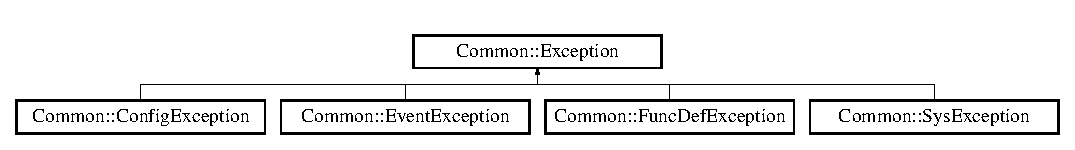
\includegraphics[height=1.573034cm]{class_common_1_1_exception}
\end{center}
\end{figure}
\subsection*{Public Member Functions}
\begin{DoxyCompactItemize}
\item 
\hyperlink{class_common_1_1_exception_a7a4159db2c3f4d33a1190135a0eb47e8}{Exception} (std\-::string const \&msg, std\-::string const \&obj\-Name=std\-::string(), long err=0)
\begin{DoxyCompactList}\small\item\em Constructor. \end{DoxyCompactList}\item 
\hypertarget{class_common_1_1_exception_acbd14afa1f0d9dfb758c0a31e7768798}{\hyperlink{class_common_1_1_exception_acbd14afa1f0d9dfb758c0a31e7768798}{Exception} ()}\label{class_common_1_1_exception_acbd14afa1f0d9dfb758c0a31e7768798}

\begin{DoxyCompactList}\small\item\em Constructor. \end{DoxyCompactList}\item 
\hypertarget{class_common_1_1_exception_aab197db6aa257d1b8cb6d68254d8e89f}{virtual \hyperlink{class_common_1_1_exception_aab197db6aa257d1b8cb6d68254d8e89f}{$\sim$\-Exception} ()}\label{class_common_1_1_exception_aab197db6aa257d1b8cb6d68254d8e89f}

\begin{DoxyCompactList}\small\item\em Destructor. \end{DoxyCompactList}\item 
\hypertarget{class_common_1_1_exception_adb47456874a4768b53b142cebdb04ccc}{long \hyperlink{class_common_1_1_exception_adb47456874a4768b53b142cebdb04ccc}{Get\-Error} () const }\label{class_common_1_1_exception_adb47456874a4768b53b142cebdb04ccc}

\begin{DoxyCompactList}\small\item\em Returns error code. \end{DoxyCompactList}\item 
\hypertarget{class_common_1_1_exception_a25042768a5180ba186b4444bcee7b59c}{std\-::string const \& \hyperlink{class_common_1_1_exception_a25042768a5180ba186b4444bcee7b59c}{Get\-Error\-Message} () const }\label{class_common_1_1_exception_a25042768a5180ba186b4444bcee7b59c}

\begin{DoxyCompactList}\small\item\em Returns error message. \end{DoxyCompactList}\item 
\hypertarget{class_common_1_1_exception_af8360d82fa52fb0ed9b3d60c8896f59e}{std\-::string const \& \hyperlink{class_common_1_1_exception_af8360d82fa52fb0ed9b3d60c8896f59e}{Get\-Object\-Name} () const }\label{class_common_1_1_exception_af8360d82fa52fb0ed9b3d60c8896f59e}

\begin{DoxyCompactList}\small\item\em Returns the name of the object. \end{DoxyCompactList}\item 
\hypertarget{class_common_1_1_exception_aedcfae1f86e9f5496c33ba4e6db883c2}{virtual void \hyperlink{class_common_1_1_exception_aedcfae1f86e9f5496c33ba4e6db883c2}{Display} () const }\label{class_common_1_1_exception_aedcfae1f86e9f5496c33ba4e6db883c2}

\begin{DoxyCompactList}\small\item\em Displays exception message on the standard error output. \end{DoxyCompactList}\item 
virtual void \hyperlink{class_common_1_1_exception_a2633eeaab3220268739977a04643a3cf}{Display} (std\-::ostream \&os) const 
\begin{DoxyCompactList}\small\item\em Displays exception message on the given output stream. \end{DoxyCompactList}\end{DoxyCompactItemize}
\subsection*{Protected Attributes}
\begin{DoxyCompactItemize}
\item 
\hypertarget{class_common_1_1_exception_a44c14e8761e67333733ff2b2496711e5}{long {\bfseries \-\_\-err}}\label{class_common_1_1_exception_a44c14e8761e67333733ff2b2496711e5}

\item 
\hypertarget{class_common_1_1_exception_a410fa237f76aae7a455f60d0e2441de2}{std\-::string {\bfseries \-\_\-msg}}\label{class_common_1_1_exception_a410fa237f76aae7a455f60d0e2441de2}

\item 
\hypertarget{class_common_1_1_exception_a3332fee5e92d992e80d28472107e7775}{std\-::string {\bfseries \-\_\-obj\-Name}}\label{class_common_1_1_exception_a3332fee5e92d992e80d28472107e7775}

\end{DoxyCompactItemize}


\subsection{Detailed Description}
Abstract class, stores information of errors on determined situations. 

\begin{DoxyVersion}{Version}
1.\-0b 
\end{DoxyVersion}
\begin{DoxySince}{Since}
1.\-0b 
\end{DoxySince}
\begin{DoxyAuthor}{Author}
Ania Sikora, 2002 
\end{DoxyAuthor}


\subsection{Constructor \& Destructor Documentation}
\hypertarget{class_common_1_1_exception_a7a4159db2c3f4d33a1190135a0eb47e8}{\index{Common\-::\-Exception@{Common\-::\-Exception}!Exception@{Exception}}
\index{Exception@{Exception}!Common::Exception@{Common\-::\-Exception}}
\subsubsection[{Exception}]{\setlength{\rightskip}{0pt plus 5cm}Common\-::\-Exception\-::\-Exception (
\begin{DoxyParamCaption}
\item[{std\-::string const \&}]{msg, }
\item[{std\-::string const \&}]{obj\-Name = {\ttfamily std\-:\-:string~()}, }
\item[{long}]{err = {\ttfamily 0}}
\end{DoxyParamCaption}
)\hspace{0.3cm}{\ttfamily [inline]}}}\label{class_common_1_1_exception_a7a4159db2c3f4d33a1190135a0eb47e8}


Constructor. 


\begin{DoxyParams}{Parameters}
{\em msg} & \hyperlink{class_common_1_1_exception}{Exception} message. \\
\hline
{\em obj\-Name} & Name of the object causing the exception, \char`\"{}\char`\"{} by default. \\
\hline
\end{DoxyParams}


\subsection{Member Function Documentation}
\hypertarget{class_common_1_1_exception_a2633eeaab3220268739977a04643a3cf}{\index{Common\-::\-Exception@{Common\-::\-Exception}!Display@{Display}}
\index{Display@{Display}!Common::Exception@{Common\-::\-Exception}}
\subsubsection[{Display}]{\setlength{\rightskip}{0pt plus 5cm}virtual void Common\-::\-Exception\-::\-Display (
\begin{DoxyParamCaption}
\item[{std\-::ostream \&}]{os}
\end{DoxyParamCaption}
) const\hspace{0.3cm}{\ttfamily [virtual]}}}\label{class_common_1_1_exception_a2633eeaab3220268739977a04643a3cf}


Displays exception message on the given output stream. 


\begin{DoxyParams}{Parameters}
{\em os} & Output stream to display the message. \\
\hline
\end{DoxyParams}


Reimplemented in \hyperlink{class_common_1_1_sys_exception_a9d45fb4b1344896490b926ccb976a7a6}{Common\-::\-Sys\-Exception}, \hyperlink{class_common_1_1_event_exception_a9f09705ed5302e3f1c0b000e10b7292a}{Common\-::\-Event\-Exception}, \hyperlink{class_common_1_1_config_exception_ad4ee85d0f156157abdde32b4fbf23369}{Common\-::\-Config\-Exception}, and \hyperlink{class_common_1_1_func_def_exception_ad9d4ee3b71921aa0d6a14bf2450897d7}{Common\-::\-Func\-Def\-Exception}.



The documentation for this class was generated from the following files\-:\begin{DoxyCompactItemize}
\item 
Common/Exception.\-h\item 
Common/Exception.\-cpp\end{DoxyCompactItemize}

\hypertarget{class_common_1_1_exec_process}{\section{Common\-:\-:Exec\-Process Class Reference}
\label{class_common_1_1_exec_process}\index{Common\-::\-Exec\-Process@{Common\-::\-Exec\-Process}}
}


Executes a program as a child of the current process.  




{\ttfamily \#include $<$Process.\-h$>$}

Inheritance diagram for Common\-:\-:Exec\-Process\-:\begin{figure}[H]
\begin{center}
\leavevmode
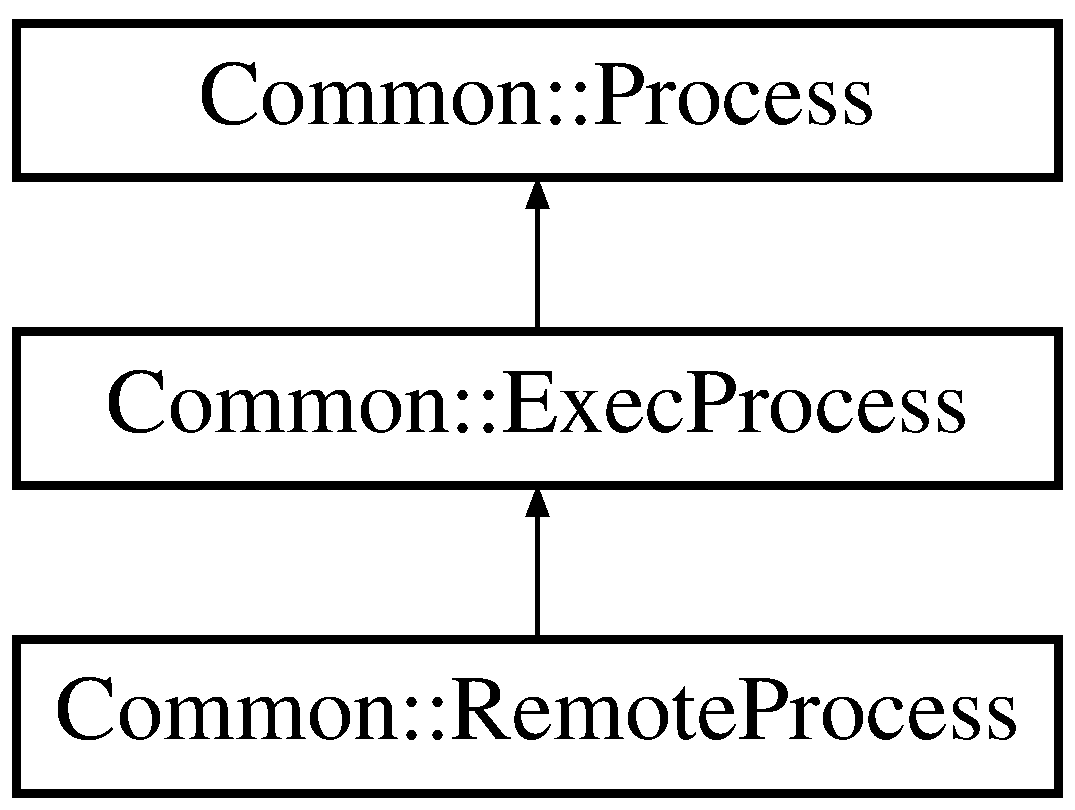
\includegraphics[height=3.000000cm]{class_common_1_1_exec_process}
\end{center}
\end{figure}
\subsection*{Public Types}
\begin{DoxyCompactItemize}
\item 
enum {\bfseries Status} \{ \\*
{\bfseries st\-Out\-Ready}, 
{\bfseries st\-Out\-Eof}, 
{\bfseries st\-Err\-Ready}, 
{\bfseries st\-Err\-Eof}, 
\\*
{\bfseries st\-Timeout}
 \}
\end{DoxyCompactItemize}
\subsection*{Public Member Functions}
\begin{DoxyCompactItemize}
\item 
\hyperlink{class_common_1_1_exec_process_a3893a568fd996514f18877b5cbf05065}{Exec\-Process} (std\-::string const \&program\-Path, char $\ast$const argv\mbox{[}$\,$\mbox{]})
\begin{DoxyCompactList}\small\item\em Constructor. \end{DoxyCompactList}\item 
void \hyperlink{class_common_1_1_exec_process_aa8771f96b42438bbcce9474fe2ad1e8f}{Start} ()
\begin{DoxyCompactList}\small\item\em Executes the program. \end{DoxyCompactList}\item 
Status \hyperlink{class_common_1_1_exec_process_a2b4ac9c756fcf3b3e9c8ddc4d6a9d5a6}{Wait\-For\-Event} (char $\ast$buffer, int buf\-Size, int \&bytes\-Read, \hyperlink{class_common_1_1_time_value}{Time\-Value} $\ast$timeout=0)
\begin{DoxyCompactList}\small\item\em Waits until an event is placed on any of the outputs of the process or the time limit is reached. \end{DoxyCompactList}\end{DoxyCompactItemize}
\subsection*{Protected Member Functions}
\begin{DoxyCompactItemize}
\item 
\hypertarget{class_common_1_1_exec_process_a2f79359e3f1c40dfc080186ddeb28379}{\hyperlink{class_common_1_1_exec_process_a2f79359e3f1c40dfc080186ddeb28379}{Exec\-Process} ()}\label{class_common_1_1_exec_process_a2f79359e3f1c40dfc080186ddeb28379}

\begin{DoxyCompactList}\small\item\em Constructor. \end{DoxyCompactList}\item 
\hypertarget{class_common_1_1_exec_process_abf41d59985934b3d78cf2e244a6fc5db}{int \hyperlink{class_common_1_1_exec_process_abf41d59985934b3d78cf2e244a6fc5db}{Run} ()}\label{class_common_1_1_exec_process_abf41d59985934b3d78cf2e244a6fc5db}

\begin{DoxyCompactList}\small\item\em Executes de process. \end{DoxyCompactList}\end{DoxyCompactItemize}
\subsection*{Additional Inherited Members}


\subsection{Detailed Description}
Executes a program as a child of the current process. 

\begin{DoxyVersion}{Version}
1.\-0b 
\end{DoxyVersion}
\begin{DoxySince}{Since}
1.\-0b 
\end{DoxySince}
\begin{DoxyAuthor}{Author}
Ania Sikora, 2001 
\end{DoxyAuthor}


\subsection{Constructor \& Destructor Documentation}
\hypertarget{class_common_1_1_exec_process_a3893a568fd996514f18877b5cbf05065}{\index{Common\-::\-Exec\-Process@{Common\-::\-Exec\-Process}!Exec\-Process@{Exec\-Process}}
\index{Exec\-Process@{Exec\-Process}!Common::ExecProcess@{Common\-::\-Exec\-Process}}
\subsubsection[{Exec\-Process}]{\setlength{\rightskip}{0pt plus 5cm}Common\-::\-Exec\-Process\-::\-Exec\-Process (
\begin{DoxyParamCaption}
\item[{std\-::string const \&}]{program\-Path, }
\item[{char $\ast$const}]{argv\mbox{[}$\,$\mbox{]}}
\end{DoxyParamCaption}
)\hspace{0.3cm}{\ttfamily [inline]}}}\label{class_common_1_1_exec_process_a3893a568fd996514f18877b5cbf05065}


Constructor. 

Example usage\-: 
\begin{DoxyCode}
\textcolor{keywordtype}{char} * argv [] = \{ \textcolor{stringliteral}{"/usr/bin/vi"}, \textcolor{stringliteral}{"param1"}, \textcolor{stringliteral}{"param2"}, 0 \};
\hyperlink{class_common_1_1_exec_process_a2f79359e3f1c40dfc080186ddeb28379}{ExecProcess} p (\textcolor{stringliteral}{"/usr/bin/vi"}, argv);
\end{DoxyCode}
 Notes\-:
\begin{DoxyItemize}
\item first element of argv must be program path
\item last element of argv table must be 0
\end{DoxyItemize}


\begin{DoxyParams}{Parameters}
{\em program\-Path} & Path of the program to execute. \\
\hline
{\em argv} & Arguments to pass to the execution of the program. \\
\hline
\end{DoxyParams}


\subsection{Member Function Documentation}
\hypertarget{class_common_1_1_exec_process_aa8771f96b42438bbcce9474fe2ad1e8f}{\index{Common\-::\-Exec\-Process@{Common\-::\-Exec\-Process}!Start@{Start}}
\index{Start@{Start}!Common::ExecProcess@{Common\-::\-Exec\-Process}}
\subsubsection[{Start}]{\setlength{\rightskip}{0pt plus 5cm}void Exec\-Process\-::\-Start (
\begin{DoxyParamCaption}
{}
\end{DoxyParamCaption}
)\hspace{0.3cm}{\ttfamily [virtual]}}}\label{class_common_1_1_exec_process_aa8771f96b42438bbcce9474fe2ad1e8f}


Executes the program. 

The standard outputs and inputs of the program will be redirected to internal pipes, to be handled on the \hyperlink{class_common_1_1_exec_process_a2b4ac9c756fcf3b3e9c8ddc4d6a9d5a6}{Wait\-For\-Event()} method. 

Reimplemented from \hyperlink{class_common_1_1_process_ae92f973fc379f7020f29d08288685c33}{Common\-::\-Process}.

\hypertarget{class_common_1_1_exec_process_a2b4ac9c756fcf3b3e9c8ddc4d6a9d5a6}{\index{Common\-::\-Exec\-Process@{Common\-::\-Exec\-Process}!Wait\-For\-Event@{Wait\-For\-Event}}
\index{Wait\-For\-Event@{Wait\-For\-Event}!Common::ExecProcess@{Common\-::\-Exec\-Process}}
\subsubsection[{Wait\-For\-Event}]{\setlength{\rightskip}{0pt plus 5cm}Exec\-Process\-::\-Status Exec\-Process\-::\-Wait\-For\-Event (
\begin{DoxyParamCaption}
\item[{char $\ast$}]{buffer, }
\item[{int}]{buf\-Size, }
\item[{int \&}]{bytes\-Read, }
\item[{{\bf Time\-Value} $\ast$}]{timeout = {\ttfamily 0}}
\end{DoxyParamCaption}
)}}\label{class_common_1_1_exec_process_a2b4ac9c756fcf3b3e9c8ddc4d6a9d5a6}


Waits until an event is placed on any of the outputs of the process or the time limit is reached. 

If any event was sent by the process, it is placed on the buffer.

\begin{DoxyReturn}{Returns}
Information about how the function ended and what was placed on the buffer. 
\end{DoxyReturn}


The documentation for this class was generated from the following files\-:\begin{DoxyCompactItemize}
\item 
Common/Process.\-h\item 
Common/Process.\-cpp\end{DoxyCompactItemize}

\hypertarget{class_factoring_tunlet}{\section{Factoring\-Tunlet Class Reference}
\label{class_factoring_tunlet}\index{Factoring\-Tunlet@{Factoring\-Tunlet}}
}


Factoring optimization tunlet for m/w apps.  




{\ttfamily \#include $<$Factoring\-Tunlet\-\_\-nw.\-h$>$}

Inheritance diagram for Factoring\-Tunlet\-:\begin{figure}[H]
\begin{center}
\leavevmode
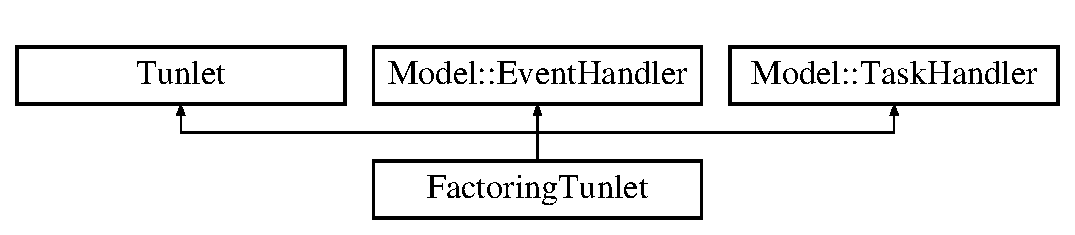
\includegraphics[height=2.000000cm]{class_factoring_tunlet}
\end{center}
\end{figure}
\subsection*{Public Member Functions}
\begin{DoxyCompactItemize}
\item 
\hypertarget{class_factoring_tunlet_a5aab3bb67f4bd4eeec882d42f96a308c}{\hyperlink{class_factoring_tunlet_a5aab3bb67f4bd4eeec882d42f96a308c}{Factoring\-Tunlet} ()}\label{class_factoring_tunlet_a5aab3bb67f4bd4eeec882d42f96a308c}

\begin{DoxyCompactList}\small\item\em Constructor. \end{DoxyCompactList}\item 
\hypertarget{class_factoring_tunlet_a0b71dcf56237028c84570a91b86ef818}{\hyperlink{class_factoring_tunlet_a0b71dcf56237028c84570a91b86ef818}{$\sim$\-Factoring\-Tunlet} ()}\label{class_factoring_tunlet_a0b71dcf56237028c84570a91b86ef818}

\begin{DoxyCompactList}\small\item\em Destructor. \end{DoxyCompactList}\item 
void \hyperlink{class_factoring_tunlet_a4883ba0a05903fb09b9f420d72927d86}{Initialize} (\hyperlink{class_model_1_1_application}{Model\-::\-Application} \&app)
\item 
\hypertarget{class_factoring_tunlet_a72678a4eaea3f9559a542cf0ffa29e03}{void \hyperlink{class_factoring_tunlet_a72678a4eaea3f9559a542cf0ffa29e03}{Before\-App\-Start} ()}\label{class_factoring_tunlet_a72678a4eaea3f9559a542cf0ffa29e03}

\begin{DoxyCompactList}\small\item\em Asserts that \-\_\-app != 0 and sets the task handler of the app to the current one. \end{DoxyCompactList}\item 
\hypertarget{class_factoring_tunlet_a3604567541e57a0dfd59d44cac44ecd2}{void \hyperlink{class_factoring_tunlet_a3604567541e57a0dfd59d44cac44ecd2}{Destroy} ()}\label{class_factoring_tunlet_a3604567541e57a0dfd59d44cac44ecd2}

\begin{DoxyCompactList}\small\item\em Sets \-\_\-app = 0. \end{DoxyCompactList}\item 
void \hyperlink{class_factoring_tunlet_aeb954297fd00f2801c807ef3ae2384f1}{Handle\-Event} (\hyperlink{class_model_1_1_event_record}{Model\-::\-Event\-Record} const \&r)
\begin{DoxyCompactList}\small\item\em Handles all incoming events. \end{DoxyCompactList}\item 
void \hyperlink{class_factoring_tunlet_ae99ec15c1e80a9fbfaf5f6e23bf8e7ef}{Task\-Started} (\hyperlink{class_model_1_1_task}{Model\-::\-Task} \&t)
\begin{DoxyCompactList}\small\item\em Increments the number of workers by 1 and inserts an event to the worker. \end{DoxyCompactList}\item 
void \hyperlink{class_factoring_tunlet_a08e03f7b58081ee5477af2fd47a5844a}{Task\-Terminated} (\hyperlink{class_model_1_1_task}{Model\-::\-Task} \&t)
\begin{DoxyCompactList}\small\item\em Decrements the number of workers by 1. \end{DoxyCompactList}\item 
\hypertarget{class_factoring_tunlet_a03bee1e1e468cb8cd2a4aacd7d5fd7de}{void \hyperlink{class_factoring_tunlet_a03bee1e1e468cb8cd2a4aacd7d5fd7de}{Create\-Event} ()}\label{class_factoring_tunlet_a03bee1e1e468cb8cd2a4aacd7d5fd7de}

\begin{DoxyCompactList}\small\item\em Creates events by using the configuration specified in the file tunlet.\-ini. \end{DoxyCompactList}\item 
void \hyperlink{class_factoring_tunlet_ad91b45da36e3a108d74bb43fd98c7683}{Create\-Event} (\hyperlink{class_model_1_1_task}{Model\-::\-Task} \&t)
\begin{DoxyCompactList}\small\item\em Creates events by using the configuration specified in the file tunlet.\-ini and a given task. \end{DoxyCompactList}\end{DoxyCompactItemize}


\subsection{Detailed Description}
Factoring optimization tunlet for m/w apps. 

\subsection{Member Function Documentation}
\hypertarget{class_factoring_tunlet_ad91b45da36e3a108d74bb43fd98c7683}{\index{Factoring\-Tunlet@{Factoring\-Tunlet}!Create\-Event@{Create\-Event}}
\index{Create\-Event@{Create\-Event}!FactoringTunlet@{Factoring\-Tunlet}}
\subsubsection[{Create\-Event}]{\setlength{\rightskip}{0pt plus 5cm}void Factoring\-Tunlet\-::\-Create\-Event (
\begin{DoxyParamCaption}
\item[{{\bf Model\-::\-Task} \&}]{t}
\end{DoxyParamCaption}
)}}\label{class_factoring_tunlet_ad91b45da36e3a108d74bb43fd98c7683}


Creates events by using the configuration specified in the file tunlet.\-ini and a given task. 


\begin{DoxyParams}{Parameters}
{\em t} & \hyperlink{class_task}{Task} \\
\hline
\end{DoxyParams}
\hypertarget{class_factoring_tunlet_aeb954297fd00f2801c807ef3ae2384f1}{\index{Factoring\-Tunlet@{Factoring\-Tunlet}!Handle\-Event@{Handle\-Event}}
\index{Handle\-Event@{Handle\-Event}!FactoringTunlet@{Factoring\-Tunlet}}
\subsubsection[{Handle\-Event}]{\setlength{\rightskip}{0pt plus 5cm}void Factoring\-Tunlet\-::\-Handle\-Event (
\begin{DoxyParamCaption}
\item[{{\bf Model\-::\-Event\-Record} const \&}]{r}
\end{DoxyParamCaption}
)\hspace{0.3cm}{\ttfamily [virtual]}}}\label{class_factoring_tunlet_aeb954297fd00f2801c807ef3ae2384f1}


Handles all incoming events. 


\begin{DoxyParams}{Parameters}
{\em r} & Event\-Record where its I\-D can be found \\
\hline
\end{DoxyParams}


Implements \hyperlink{class_model_1_1_event_handler_a0a84c727f41c358350a2f3522ffba03b}{Model\-::\-Event\-Handler}.

\hypertarget{class_factoring_tunlet_a4883ba0a05903fb09b9f420d72927d86}{\index{Factoring\-Tunlet@{Factoring\-Tunlet}!Initialize@{Initialize}}
\index{Initialize@{Initialize}!FactoringTunlet@{Factoring\-Tunlet}}
\subsubsection[{Initialize}]{\setlength{\rightskip}{0pt plus 5cm}void Factoring\-Tunlet\-::\-Initialize (
\begin{DoxyParamCaption}
\item[{{\bf Model\-::\-Application} \&}]{app}
\end{DoxyParamCaption}
)\hspace{0.3cm}{\ttfamily [virtual]}}}\label{class_factoring_tunlet_a4883ba0a05903fb09b9f420d72927d86}

\begin{DoxyParams}{Parameters}
{\em app} & \\
\hline
\end{DoxyParams}


Implements \hyperlink{class_tunlet_aeb84d0844192764dc9aef3cb905c4e7e}{Tunlet}.

\hypertarget{class_factoring_tunlet_ae99ec15c1e80a9fbfaf5f6e23bf8e7ef}{\index{Factoring\-Tunlet@{Factoring\-Tunlet}!Task\-Started@{Task\-Started}}
\index{Task\-Started@{Task\-Started}!FactoringTunlet@{Factoring\-Tunlet}}
\subsubsection[{Task\-Started}]{\setlength{\rightskip}{0pt plus 5cm}void Factoring\-Tunlet\-::\-Task\-Started (
\begin{DoxyParamCaption}
\item[{{\bf Model\-::\-Task} \&}]{t}
\end{DoxyParamCaption}
)\hspace{0.3cm}{\ttfamily [virtual]}}}\label{class_factoring_tunlet_ae99ec15c1e80a9fbfaf5f6e23bf8e7ef}


Increments the number of workers by 1 and inserts an event to the worker. 


\begin{DoxyParams}{Parameters}
{\em t} & \hyperlink{class_task}{Task} \\
\hline
\end{DoxyParams}


Implements \hyperlink{class_model_1_1_task_handler_a357c8d730fd4e95582f99046d3474dae}{Model\-::\-Task\-Handler}.

\hypertarget{class_factoring_tunlet_a08e03f7b58081ee5477af2fd47a5844a}{\index{Factoring\-Tunlet@{Factoring\-Tunlet}!Task\-Terminated@{Task\-Terminated}}
\index{Task\-Terminated@{Task\-Terminated}!FactoringTunlet@{Factoring\-Tunlet}}
\subsubsection[{Task\-Terminated}]{\setlength{\rightskip}{0pt plus 5cm}void Factoring\-Tunlet\-::\-Task\-Terminated (
\begin{DoxyParamCaption}
\item[{{\bf Model\-::\-Task} \&}]{t}
\end{DoxyParamCaption}
)\hspace{0.3cm}{\ttfamily [virtual]}}}\label{class_factoring_tunlet_a08e03f7b58081ee5477af2fd47a5844a}


Decrements the number of workers by 1. 


\begin{DoxyParams}{Parameters}
{\em t} & \hyperlink{class_task}{Task} \\
\hline
\end{DoxyParams}


Implements \hyperlink{class_model_1_1_task_handler_a7c19d0ad21f0cd431ee31f022a7455b7}{Model\-::\-Task\-Handler}.



The documentation for this class was generated from the following files\-:\begin{DoxyCompactItemize}
\item 
Analyzer/Factoring\-Tunlet\-\_\-nw.\-h\item 
Analyzer/Factoring\-Tunlet\-\_\-nw-\/\-X\-Fire.\-cpp\item 
Analyzer/Factoring\-Tunlet\-\_\-nw.\-cpp\end{DoxyCompactItemize}

\hypertarget{class_common_1_1_file_config_reader}{\section{Common\-:\-:File\-Config\-Reader Class Reference}
\label{class_common_1_1_file_config_reader}\index{Common\-::\-File\-Config\-Reader@{Common\-::\-File\-Config\-Reader}}
}


Parses the content of a file into a \hyperlink{class_common_1_1_config}{Config} object.  




{\ttfamily \#include $<$Config\-Reader.\-h$>$}

Inheritance diagram for Common\-:\-:File\-Config\-Reader\-:\begin{figure}[H]
\begin{center}
\leavevmode
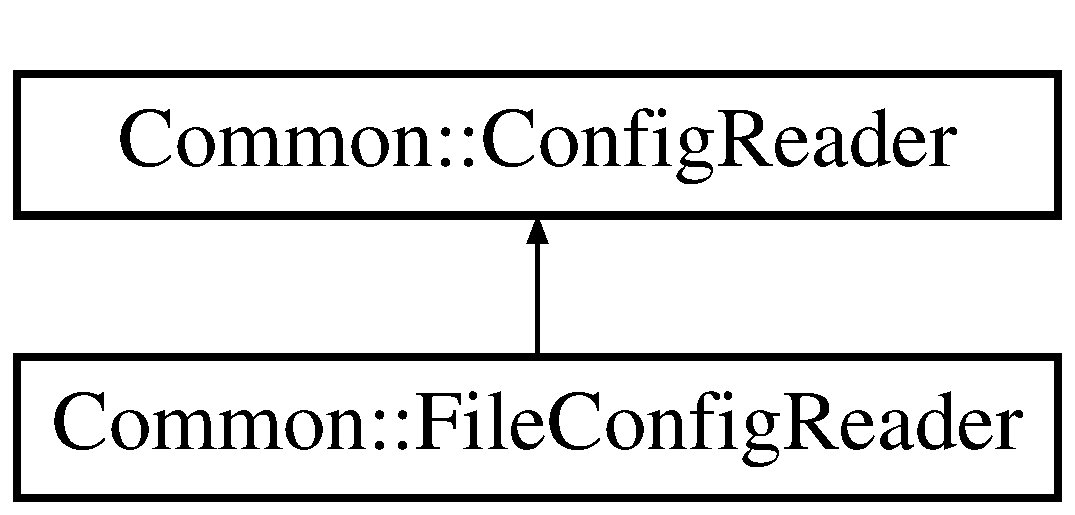
\includegraphics[height=2.000000cm]{class_common_1_1_file_config_reader}
\end{center}
\end{figure}
\subsection*{Public Member Functions}
\begin{DoxyCompactItemize}
\item 
\hyperlink{class_common_1_1_file_config_reader_adfdd8100b30811cf8a1800e48fe6e037}{File\-Config\-Reader} (std\-::string const \&file\-Name)
\begin{DoxyCompactList}\small\item\em Constructor. \end{DoxyCompactList}\item 
\hyperlink{class_common_1_1_config}{Config} \hyperlink{class_common_1_1_file_config_reader_a8ef84330b129aa44ad36c6de827d4cad}{Read} ()
\begin{DoxyCompactList}\small\item\em Parses the configuration of the file into a \hyperlink{class_common_1_1_config}{Config} object. \end{DoxyCompactList}\end{DoxyCompactItemize}
\subsection*{Additional Inherited Members}


\subsection{Detailed Description}
Parses the content of a file into a \hyperlink{class_common_1_1_config}{Config} object. 

Extends \hyperlink{class_common_1_1_config_reader}{Config\-Reader}

\begin{DoxyVersion}{Version}
1.\-0b 
\end{DoxyVersion}
\begin{DoxySince}{Since}
1.\-0b 
\end{DoxySince}
\begin{DoxyAuthor}{Author}
Noel De Martin, 2011 
\end{DoxyAuthor}


\subsection{Constructor \& Destructor Documentation}
\hypertarget{class_common_1_1_file_config_reader_adfdd8100b30811cf8a1800e48fe6e037}{\index{Common\-::\-File\-Config\-Reader@{Common\-::\-File\-Config\-Reader}!File\-Config\-Reader@{File\-Config\-Reader}}
\index{File\-Config\-Reader@{File\-Config\-Reader}!Common::FileConfigReader@{Common\-::\-File\-Config\-Reader}}
\subsubsection[{File\-Config\-Reader}]{\setlength{\rightskip}{0pt plus 5cm}Common\-::\-File\-Config\-Reader\-::\-File\-Config\-Reader (
\begin{DoxyParamCaption}
\item[{std\-::string const \&}]{file\-Name}
\end{DoxyParamCaption}
)\hspace{0.3cm}{\ttfamily [inline]}}}\label{class_common_1_1_file_config_reader_adfdd8100b30811cf8a1800e48fe6e037}


Constructor. 


\begin{DoxyParams}{Parameters}
{\em file\-Name} & Path of the file to read.\\
\hline
\end{DoxyParams}

\begin{DoxyExceptions}{Exceptions}
{\em \hyperlink{class_common_1_1_config_exception}{Config\-Exception}} & \\
\hline
\end{DoxyExceptions}


\subsection{Member Function Documentation}
\hypertarget{class_common_1_1_file_config_reader_a8ef84330b129aa44ad36c6de827d4cad}{\index{Common\-::\-File\-Config\-Reader@{Common\-::\-File\-Config\-Reader}!Read@{Read}}
\index{Read@{Read}!Common::FileConfigReader@{Common\-::\-File\-Config\-Reader}}
\subsubsection[{Read}]{\setlength{\rightskip}{0pt plus 5cm}{\bf Config} File\-Config\-Reader\-::\-Read (
\begin{DoxyParamCaption}
{}
\end{DoxyParamCaption}
)\hspace{0.3cm}{\ttfamily [virtual]}}}\label{class_common_1_1_file_config_reader_a8ef84330b129aa44ad36c6de827d4cad}


Parses the configuration of the file into a \hyperlink{class_common_1_1_config}{Config} object. 


\begin{DoxyExceptions}{Exceptions}
{\em \hyperlink{class_common_1_1_config_exception}{Config\-Exception}} & \\
\hline
\end{DoxyExceptions}


Implements \hyperlink{class_common_1_1_config_reader}{Common\-::\-Config\-Reader}.



The documentation for this class was generated from the following files\-:\begin{DoxyCompactItemize}
\item 
Common/Config\-Reader.\-h\item 
Common/Config\-Reader.\-cpp\end{DoxyCompactItemize}

\hypertarget{class_common_1_1_file_logger}{\section{Common\-:\-:File\-Logger Class Reference}
\label{class_common_1_1_file_logger}\index{Common\-::\-File\-Logger@{Common\-::\-File\-Logger}}
}


Stores information of interest into a file.  




{\ttfamily \#include $<$Syslog.\-h$>$}

Inheritance diagram for Common\-:\-:File\-Logger\-:\begin{figure}[H]
\begin{center}
\leavevmode
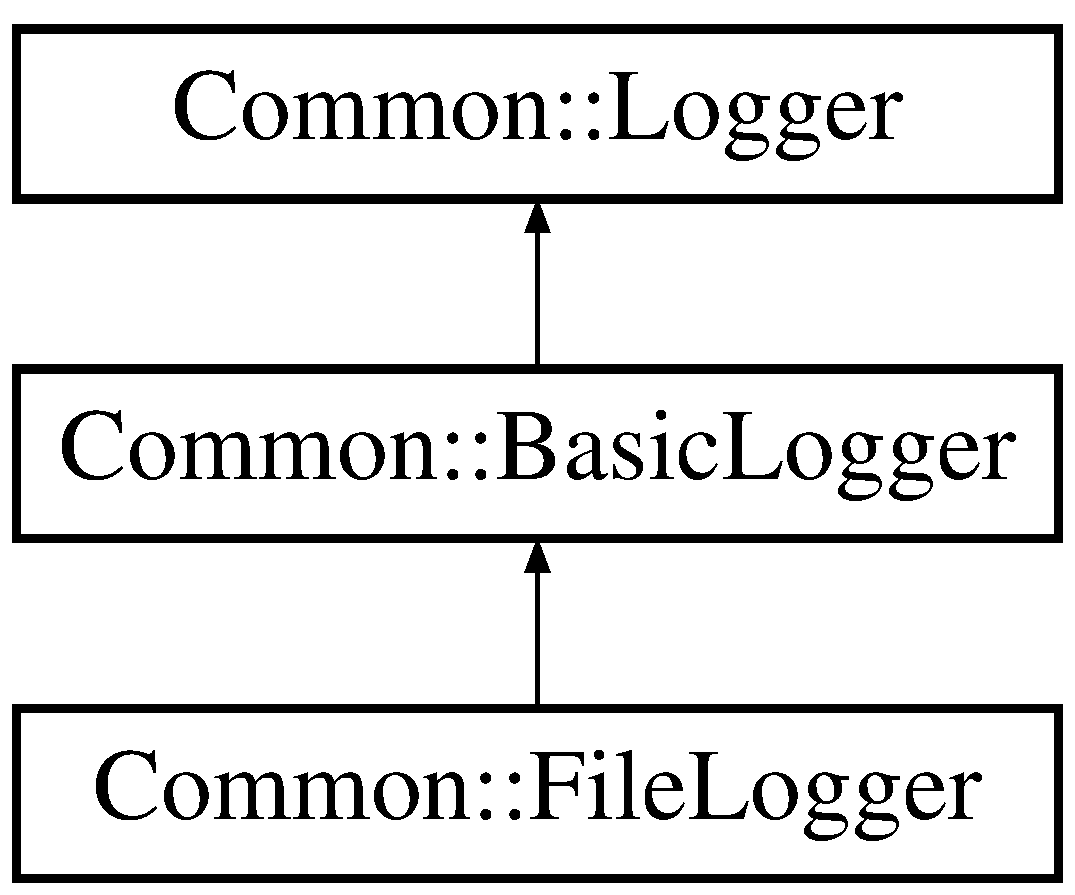
\includegraphics[height=3.000000cm]{class_common_1_1_file_logger}
\end{center}
\end{figure}
\subsection*{Public Member Functions}
\begin{DoxyCompactItemize}
\item 
\hyperlink{class_common_1_1_file_logger_a23395819e1621d8825a9685fbc61857c}{File\-Logger} (std\-::string const \&filepath, bool append=false)
\begin{DoxyCompactList}\small\item\em Constructor. \end{DoxyCompactList}\item 
\hypertarget{class_common_1_1_file_logger_ab08af44f2de3fe1b51158132f9a399dd}{\hyperlink{class_common_1_1_file_logger_ab08af44f2de3fe1b51158132f9a399dd}{$\sim$\-File\-Logger} ()}\label{class_common_1_1_file_logger_ab08af44f2de3fe1b51158132f9a399dd}

\begin{DoxyCompactList}\small\item\em Destructor. \end{DoxyCompactList}\item 
\hypertarget{class_common_1_1_file_logger_a2f487ff3e7c10476f371e5cc7166a6f3}{void \hyperlink{class_common_1_1_file_logger_a2f487ff3e7c10476f371e5cc7166a6f3}{Log} (\hyperlink{class_common_1_1_log_entry}{Log\-Entry} const \&entry)}\label{class_common_1_1_file_logger_a2f487ff3e7c10476f371e5cc7166a6f3}

\begin{DoxyCompactList}\small\item\em Inserts a new entry to the log. \end{DoxyCompactList}\end{DoxyCompactItemize}
\subsection*{Additional Inherited Members}


\subsection{Detailed Description}
Stores information of interest into a file. 

\begin{DoxyVersion}{Version}
1.\-0b 
\end{DoxyVersion}
\begin{DoxySince}{Since}
1.\-0b 
\end{DoxySince}
\begin{DoxyAuthor}{Author}
Ania Sikora, 2002 
\end{DoxyAuthor}


\subsection{Constructor \& Destructor Documentation}
\hypertarget{class_common_1_1_file_logger_a23395819e1621d8825a9685fbc61857c}{\index{Common\-::\-File\-Logger@{Common\-::\-File\-Logger}!File\-Logger@{File\-Logger}}
\index{File\-Logger@{File\-Logger}!Common::FileLogger@{Common\-::\-File\-Logger}}
\subsubsection[{File\-Logger}]{\setlength{\rightskip}{0pt plus 5cm}File\-Logger\-::\-File\-Logger (
\begin{DoxyParamCaption}
\item[{std\-::string const \&}]{filepath, }
\item[{bool}]{append = {\ttfamily false}}
\end{DoxyParamCaption}
)}}\label{class_common_1_1_file_logger_a23395819e1621d8825a9685fbc61857c}


Constructor. 


\begin{DoxyParams}{Parameters}
{\em filepath} & Path of the file where the log will be stored.  append Flag that determines if the file will be overwritten or the logs will be appended, default false.\\
\hline
\end{DoxyParams}

\begin{DoxyExceptions}{Exceptions}
{\em \hyperlink{class_common_1_1_sys_exception}{Sys\-Exception}} & \\
\hline
\end{DoxyExceptions}


The documentation for this class was generated from the following files\-:\begin{DoxyCompactItemize}
\item 
Common/Syslog.\-h\item 
Common/Syslog.\-cpp\end{DoxyCompactItemize}

\hypertarget{class_common_1_1_func_def}{\section{Common\-:\-:Func\-Def Class Reference}
\label{class_common_1_1_func_def}\index{Common\-::\-Func\-Def@{Common\-::\-Func\-Def}}
}


Represents definition of the function to be traced.  




{\ttfamily \#include $<$Func\-Defs.\-h$>$}

\subsection*{Public Member Functions}
\begin{DoxyCompactItemize}
\item 
\hyperlink{class_common_1_1_func_def_a8a61bdb6eaf3f205d5ed8357d7a79e86}{Func\-Def} (std\-::string const \&name, std\-::string const \&param\-Format, int param\-Count, int func\-Id)
\begin{DoxyCompactList}\small\item\em Constructor. \end{DoxyCompactList}\item 
\hypertarget{class_common_1_1_func_def_a4a9f4c8c0ec7e96f4084c50b15e08f12}{std\-::string const \& \hyperlink{class_common_1_1_func_def_a4a9f4c8c0ec7e96f4084c50b15e08f12}{Get\-Name} () const }\label{class_common_1_1_func_def_a4a9f4c8c0ec7e96f4084c50b15e08f12}

\begin{DoxyCompactList}\small\item\em Returns name of the function. \end{DoxyCompactList}\item 
\hypertarget{class_common_1_1_func_def_a062193e6cd4c8d8618d1b55b3edc2198}{std\-::string const \& \hyperlink{class_common_1_1_func_def_a062193e6cd4c8d8618d1b55b3edc2198}{Get\-Param\-Format} () const }\label{class_common_1_1_func_def_a062193e6cd4c8d8618d1b55b3edc2198}

\begin{DoxyCompactList}\small\item\em Returns format of the parameters. \end{DoxyCompactList}\item 
\hypertarget{class_common_1_1_func_def_a92d64c6e41922738cd79c8c111c8ded9}{int \hyperlink{class_common_1_1_func_def_a92d64c6e41922738cd79c8c111c8ded9}{Get\-Param\-Count} () const }\label{class_common_1_1_func_def_a92d64c6e41922738cd79c8c111c8ded9}

\begin{DoxyCompactList}\small\item\em Returns number of parameters used by the function. \end{DoxyCompactList}\item 
\hypertarget{class_common_1_1_func_def_a1c3dfe1b838c37f70c0b2ad0958a5dd5}{int \hyperlink{class_common_1_1_func_def_a1c3dfe1b838c37f70c0b2ad0958a5dd5}{Get\-Func\-Id} () const }\label{class_common_1_1_func_def_a1c3dfe1b838c37f70c0b2ad0958a5dd5}

\begin{DoxyCompactList}\small\item\em Returns Id of the function. \end{DoxyCompactList}\end{DoxyCompactItemize}


\subsection{Detailed Description}
Represents definition of the function to be traced. 

\begin{DoxyVersion}{Version}
1.\-0b 
\end{DoxyVersion}
\begin{DoxySince}{Since}
1.\-0b 
\end{DoxySince}
\begin{DoxyAuthor}{Author}
Ania Sikora, 2003 
\end{DoxyAuthor}


\subsection{Constructor \& Destructor Documentation}
\hypertarget{class_common_1_1_func_def_a8a61bdb6eaf3f205d5ed8357d7a79e86}{\index{Common\-::\-Func\-Def@{Common\-::\-Func\-Def}!Func\-Def@{Func\-Def}}
\index{Func\-Def@{Func\-Def}!Common::FuncDef@{Common\-::\-Func\-Def}}
\subsubsection[{Func\-Def}]{\setlength{\rightskip}{0pt plus 5cm}Common\-::\-Func\-Def\-::\-Func\-Def (
\begin{DoxyParamCaption}
\item[{std\-::string const \&}]{name, }
\item[{std\-::string const \&}]{param\-Format, }
\item[{int}]{param\-Count, }
\item[{int}]{func\-Id}
\end{DoxyParamCaption}
)\hspace{0.3cm}{\ttfamily [inline]}}}\label{class_common_1_1_func_def_a8a61bdb6eaf3f205d5ed8357d7a79e86}


Constructor. 


\begin{DoxyParams}{Parameters}
{\em name} & Name of the function \\
\hline
{\em param\-Format} & String denoting types of the parameters. S\-: String, I\-: Integer, P\-: Pointer. \\
\hline
{\em param\-Count} & Number of parameters. \\
\hline
{\em func\-Id} & Function Id. \\
\hline
\end{DoxyParams}


The documentation for this class was generated from the following file\-:\begin{DoxyCompactItemize}
\item 
Common/Func\-Defs.\-h\end{DoxyCompactItemize}

\hypertarget{class_common_1_1_func_def_exception}{\section{Common\-:\-:Func\-Def\-Exception Class Reference}
\label{class_common_1_1_func_def_exception}\index{Common\-::\-Func\-Def\-Exception@{Common\-::\-Func\-Def\-Exception}}
}


\hyperlink{class_common_1_1_func_def}{Func\-Def} exceptions.  




{\ttfamily \#include $<$Func\-Def\-Exception.\-h$>$}

Inheritance diagram for Common\-:\-:Func\-Def\-Exception\-:\begin{figure}[H]
\begin{center}
\leavevmode
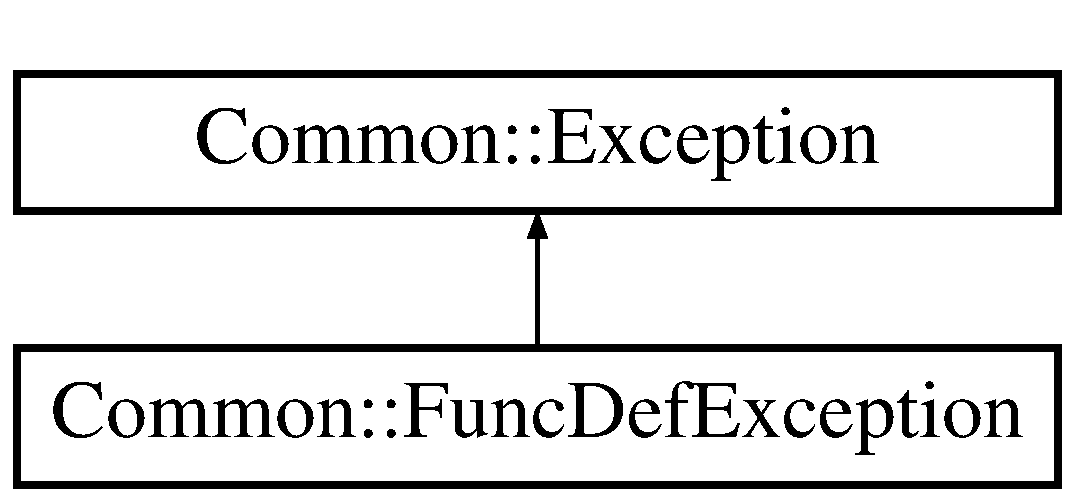
\includegraphics[height=2.000000cm]{class_common_1_1_func_def_exception}
\end{center}
\end{figure}
\subsection*{Public Member Functions}
\begin{DoxyCompactItemize}
\item 
\hyperlink{class_common_1_1_func_def_exception_aa06c459c9c9ad9ea53b4495f03bb5e0c}{Func\-Def\-Exception} (std\-::string const \&msg, std\-::string const \&obj\-Name=std\-::string())
\begin{DoxyCompactList}\small\item\em Constructor. \end{DoxyCompactList}\item 
void \hyperlink{class_common_1_1_func_def_exception_ad9d4ee3b71921aa0d6a14bf2450897d7}{Display} (std\-::ostream \&os) const 
\begin{DoxyCompactList}\small\item\em Displays exception message on the given output stream. \end{DoxyCompactList}\item 
\hypertarget{class_common_1_1_func_def_exception_aa21acc3ca2cb91020c58668990dbd210}{void \hyperlink{class_common_1_1_func_def_exception_aa21acc3ca2cb91020c58668990dbd210}{Display} () const }\label{class_common_1_1_func_def_exception_aa21acc3ca2cb91020c58668990dbd210}

\begin{DoxyCompactList}\small\item\em Displays exception message on the standard error output. \end{DoxyCompactList}\item 
std\-::string \hyperlink{class_common_1_1_func_def_exception_a254c77c993c8ee0b286d2720b255f4b7}{Get\-Reason} () const 
\begin{DoxyCompactList}\small\item\em Returns a string containing the error message. \end{DoxyCompactList}\end{DoxyCompactItemize}
\subsection*{Additional Inherited Members}


\subsection{Detailed Description}
\hyperlink{class_common_1_1_func_def}{Func\-Def} exceptions. 

\begin{DoxyVersion}{Version}
1.\-0b 
\end{DoxyVersion}
\begin{DoxySince}{Since}
1.\-0b 
\end{DoxySince}
\begin{DoxyAuthor}{Author}
Noel De Martin, 2011 
\end{DoxyAuthor}


\subsection{Constructor \& Destructor Documentation}
\hypertarget{class_common_1_1_func_def_exception_aa06c459c9c9ad9ea53b4495f03bb5e0c}{\index{Common\-::\-Func\-Def\-Exception@{Common\-::\-Func\-Def\-Exception}!Func\-Def\-Exception@{Func\-Def\-Exception}}
\index{Func\-Def\-Exception@{Func\-Def\-Exception}!Common::FuncDefException@{Common\-::\-Func\-Def\-Exception}}
\subsubsection[{Func\-Def\-Exception}]{\setlength{\rightskip}{0pt plus 5cm}Common\-::\-Func\-Def\-Exception\-::\-Func\-Def\-Exception (
\begin{DoxyParamCaption}
\item[{std\-::string const \&}]{msg, }
\item[{std\-::string const \&}]{obj\-Name = {\ttfamily std\-:\-:string~()}}
\end{DoxyParamCaption}
)\hspace{0.3cm}{\ttfamily [inline]}}}\label{class_common_1_1_func_def_exception_aa06c459c9c9ad9ea53b4495f03bb5e0c}


Constructor. 


\begin{DoxyParams}{Parameters}
{\em msg} & \hyperlink{class_common_1_1_exception}{Exception} message. \\
\hline
{\em obj\-Name} & Name of the object causing the exception, \char`\"{}\char`\"{} by default. \\
\hline
\end{DoxyParams}


\subsection{Member Function Documentation}
\hypertarget{class_common_1_1_func_def_exception_ad9d4ee3b71921aa0d6a14bf2450897d7}{\index{Common\-::\-Func\-Def\-Exception@{Common\-::\-Func\-Def\-Exception}!Display@{Display}}
\index{Display@{Display}!Common::FuncDefException@{Common\-::\-Func\-Def\-Exception}}
\subsubsection[{Display}]{\setlength{\rightskip}{0pt plus 5cm}void Func\-Def\-Exception\-::\-Display (
\begin{DoxyParamCaption}
\item[{std\-::ostream \&}]{os}
\end{DoxyParamCaption}
) const\hspace{0.3cm}{\ttfamily [virtual]}}}\label{class_common_1_1_func_def_exception_ad9d4ee3b71921aa0d6a14bf2450897d7}


Displays exception message on the given output stream. 


\begin{DoxyParams}{Parameters}
{\em os} & Output stream to display the message. \\
\hline
\end{DoxyParams}


Reimplemented from \hyperlink{class_common_1_1_exception_a2633eeaab3220268739977a04643a3cf}{Common\-::\-Exception}.

\hypertarget{class_common_1_1_func_def_exception_a254c77c993c8ee0b286d2720b255f4b7}{\index{Common\-::\-Func\-Def\-Exception@{Common\-::\-Func\-Def\-Exception}!Get\-Reason@{Get\-Reason}}
\index{Get\-Reason@{Get\-Reason}!Common::FuncDefException@{Common\-::\-Func\-Def\-Exception}}
\subsubsection[{Get\-Reason}]{\setlength{\rightskip}{0pt plus 5cm}string Func\-Def\-Exception\-::\-Get\-Reason (
\begin{DoxyParamCaption}
{}
\end{DoxyParamCaption}
) const}}\label{class_common_1_1_func_def_exception_a254c77c993c8ee0b286d2720b255f4b7}


Returns a string containing the error message. 

\begin{DoxyReturn}{Returns}
String with the error. 
\end{DoxyReturn}


The documentation for this class was generated from the following files\-:\begin{DoxyCompactItemize}
\item 
Common/Func\-Def\-Exception.\-h\item 
Common/Func\-Def\-Exception.\-cpp\end{DoxyCompactItemize}

\hypertarget{class_common_1_1_func_defs}{\section{Common\-:\-:Func\-Defs Class Reference}
\label{class_common_1_1_func_defs}\index{Common\-::\-Func\-Defs@{Common\-::\-Func\-Defs}}
}


Creates and stores objects of the \hyperlink{class_common_1_1_func_def}{Func\-Def} class.  




{\ttfamily \#include $<$Func\-Defs.\-h$>$}

\subsection*{Public Member Functions}
\begin{DoxyCompactItemize}
\item 
\hyperlink{class_common_1_1_func_defs_a2e75ea4865aa8274523be4b9fdc8b428}{Func\-Defs} ()
\begin{DoxyCompactList}\small\item\em Constructor. \end{DoxyCompactList}\item 
void \hyperlink{class_common_1_1_func_defs_ab849214cd5d440ab86372d724af154d3}{Add} (std\-::string const \&func\-Name, std\-::string const \&param\-Format, int param\-Count, int func\-Id)
\begin{DoxyCompactList}\small\item\em Adds a \hyperlink{class_common_1_1_func_def}{Func\-Def} object. \end{DoxyCompactList}\item 
\hyperlink{class_common_1_1_func_def}{Func\-Def} const \& \hyperlink{class_common_1_1_func_defs_a72003c3b38c4be15e493194dc1229386}{Find} (std\-::string const \&name)
\begin{DoxyCompactList}\small\item\em Returns a \hyperlink{class_common_1_1_func_def}{Func\-Def} object with the given name. \end{DoxyCompactList}\item 
\hypertarget{class_common_1_1_func_defs_a69600305351b797fa663eb03063cc615}{int \hyperlink{class_common_1_1_func_defs_a69600305351b797fa663eb03063cc615}{Get\-Size} () const }\label{class_common_1_1_func_defs_a69600305351b797fa663eb03063cc615}

\begin{DoxyCompactList}\small\item\em Returns number of \hyperlink{class_common_1_1_func_def}{Func\-Def} objects stored. \end{DoxyCompactList}\end{DoxyCompactItemize}


\subsection{Detailed Description}
Creates and stores objects of the \hyperlink{class_common_1_1_func_def}{Func\-Def} class. 

\begin{DoxyVersion}{Version}
1.\-0b 
\end{DoxyVersion}
\begin{DoxySince}{Since}
1.\-0b 
\end{DoxySince}
\begin{DoxyAuthor}{Author}
Ania Sikora, 2003 
\end{DoxyAuthor}


\subsection{Constructor \& Destructor Documentation}
\hypertarget{class_common_1_1_func_defs_a2e75ea4865aa8274523be4b9fdc8b428}{\index{Common\-::\-Func\-Defs@{Common\-::\-Func\-Defs}!Func\-Defs@{Func\-Defs}}
\index{Func\-Defs@{Func\-Defs}!Common::FuncDefs@{Common\-::\-Func\-Defs}}
\subsubsection[{Func\-Defs}]{\setlength{\rightskip}{0pt plus 5cm}Func\-Defs\-::\-Func\-Defs (
\begin{DoxyParamCaption}
{}
\end{DoxyParamCaption}
)}}\label{class_common_1_1_func_defs_a2e75ea4865aa8274523be4b9fdc8b428}


Constructor. 


\begin{DoxyExceptions}{Exceptions}
{\em \hyperlink{class_common_1_1_func_def_exception}{Func\-Def\-Exception}} & \\
\hline
\end{DoxyExceptions}


\subsection{Member Function Documentation}
\hypertarget{class_common_1_1_func_defs_ab849214cd5d440ab86372d724af154d3}{\index{Common\-::\-Func\-Defs@{Common\-::\-Func\-Defs}!Add@{Add}}
\index{Add@{Add}!Common::FuncDefs@{Common\-::\-Func\-Defs}}
\subsubsection[{Add}]{\setlength{\rightskip}{0pt plus 5cm}void Func\-Defs\-::\-Add (
\begin{DoxyParamCaption}
\item[{std\-::string const \&}]{func\-Name, }
\item[{std\-::string const \&}]{param\-Format, }
\item[{int}]{param\-Count, }
\item[{int}]{func\-Id}
\end{DoxyParamCaption}
)}}\label{class_common_1_1_func_defs_ab849214cd5d440ab86372d724af154d3}


Adds a \hyperlink{class_common_1_1_func_def}{Func\-Def} object. 

Uses the default constructor of \hyperlink{class_common_1_1_func_def}{Func\-Def} with the given parameters.


\begin{DoxyExceptions}{Exceptions}
{\em \hyperlink{class_common_1_1_func_def_exception}{Func\-Def\-Exception}} & \\
\hline
\end{DoxyExceptions}
\hypertarget{class_common_1_1_func_defs_a72003c3b38c4be15e493194dc1229386}{\index{Common\-::\-Func\-Defs@{Common\-::\-Func\-Defs}!Find@{Find}}
\index{Find@{Find}!Common::FuncDefs@{Common\-::\-Func\-Defs}}
\subsubsection[{Find}]{\setlength{\rightskip}{0pt plus 5cm}{\bf Func\-Def} const \& Func\-Defs\-::\-Find (
\begin{DoxyParamCaption}
\item[{std\-::string const \&}]{name}
\end{DoxyParamCaption}
)}}\label{class_common_1_1_func_defs_a72003c3b38c4be15e493194dc1229386}


Returns a \hyperlink{class_common_1_1_func_def}{Func\-Def} object with the given name. 


\begin{DoxyExceptions}{Exceptions}
{\em \hyperlink{class_common_1_1_func_def_exception}{Func\-Def\-Exception}} & \\
\hline
\end{DoxyExceptions}


The documentation for this class was generated from the following files\-:\begin{DoxyCompactItemize}
\item 
Common/Func\-Defs.\-h\item 
Common/Func\-Defs.\-cpp\end{DoxyCompactItemize}

\hypertarget{class_common_1_1_function_param_change_request}{\section{Common\-:\-:Function\-Param\-Change\-Request Class Reference}
\label{class_common_1_1_function_param_change_request}\index{Common\-::\-Function\-Param\-Change\-Request@{Common\-::\-Function\-Param\-Change\-Request}}
}


Encapsulates a tuning request to set the value of an input parameter of a given function in a given application process.  




{\ttfamily \#include $<$P\-T\-P\-Msg.\-h$>$}

Inheritance diagram for Common\-:\-:Function\-Param\-Change\-Request\-:\begin{figure}[H]
\begin{center}
\leavevmode
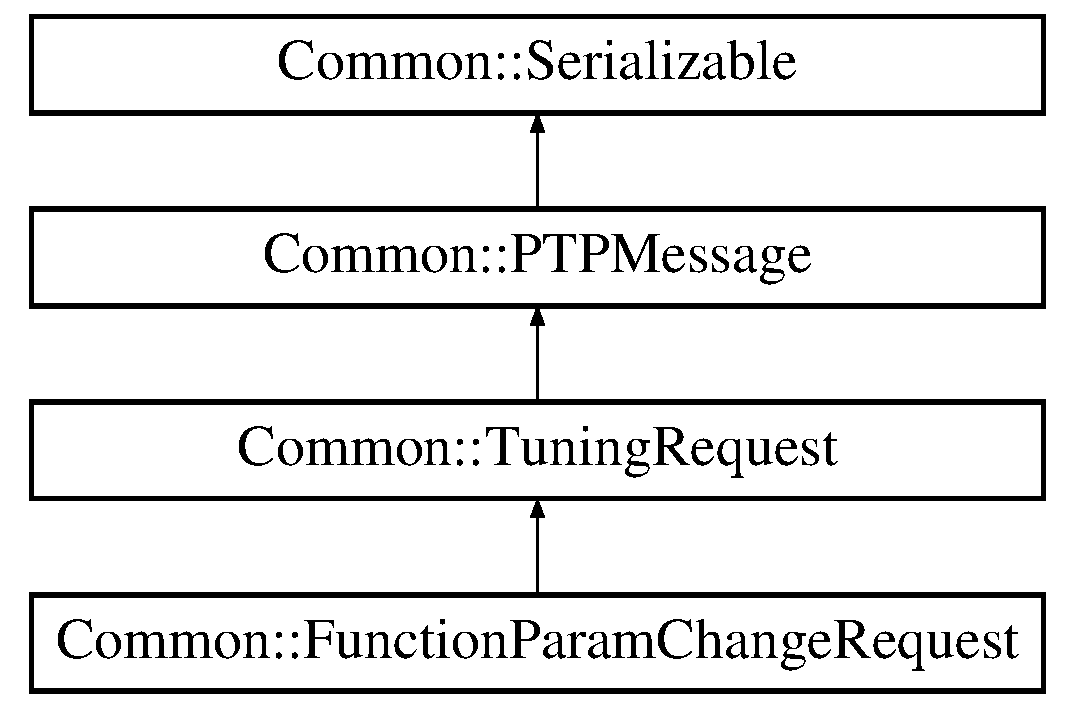
\includegraphics[height=4.000000cm]{class_common_1_1_function_param_change_request}
\end{center}
\end{figure}
\subsection*{Public Member Functions}
\begin{DoxyCompactItemize}
\item 
\hyperlink{class_common_1_1_function_param_change_request_af7dda136dbc498eee347e102b7660e05}{Function\-Param\-Change\-Request} (int pid=0, std\-::string const \&func\-Name=std\-::string(), int param\-Idx=0, int new\-Value=0, int $\ast$required\-Old\-Value=0, \hyperlink{class_common_1_1_breakpoint}{Breakpoint} $\ast$brkpt=0)
\begin{DoxyCompactList}\small\item\em Constructor. \end{DoxyCompactList}\item 
\hypertarget{class_common_1_1_function_param_change_request_a83084a194eab68eefac8f252f6069544}{P\-T\-P\-Msg\-Type \hyperlink{class_common_1_1_function_param_change_request_a83084a194eab68eefac8f252f6069544}{Get\-Type} () const }\label{class_common_1_1_function_param_change_request_a83084a194eab68eefac8f252f6069544}

\begin{DoxyCompactList}\small\item\em Returns type of message (P\-T\-P\-Func\-Param\-Change). \end{DoxyCompactList}\item 
\hypertarget{class_common_1_1_function_param_change_request_a4145f87ead31be5fefae3162497ea82d}{std\-::string const \& \hyperlink{class_common_1_1_function_param_change_request_a4145f87ead31be5fefae3162497ea82d}{Get\-Func\-Name} () const }\label{class_common_1_1_function_param_change_request_a4145f87ead31be5fefae3162497ea82d}

\begin{DoxyCompactList}\small\item\em Returns name of the function. \end{DoxyCompactList}\item 
\hypertarget{class_common_1_1_function_param_change_request_a97469c4fb80293552d3f541aef95e1c4}{int \hyperlink{class_common_1_1_function_param_change_request_a97469c4fb80293552d3f541aef95e1c4}{Get\-Param\-Idx} () const }\label{class_common_1_1_function_param_change_request_a97469c4fb80293552d3f541aef95e1c4}

\begin{DoxyCompactList}\small\item\em Returns index of the parameter to change on the attributes array. \end{DoxyCompactList}\item 
\hypertarget{class_common_1_1_function_param_change_request_a38fab3169cc0a5376eb08a3a548c84b3}{int \hyperlink{class_common_1_1_function_param_change_request_a38fab3169cc0a5376eb08a3a548c84b3}{Get\-New\-Value} () const }\label{class_common_1_1_function_param_change_request_a38fab3169cc0a5376eb08a3a548c84b3}

\begin{DoxyCompactList}\small\item\em Returns the new value to replace on the function call. \end{DoxyCompactList}\item 
\hypertarget{class_common_1_1_function_param_change_request_ace9a5ed080c6acc0f672dadb3ecf5b5c}{int const $\ast$ \hyperlink{class_common_1_1_function_param_change_request_ace9a5ed080c6acc0f672dadb3ecf5b5c}{Get\-Req\-Old\-Value} () const }\label{class_common_1_1_function_param_change_request_ace9a5ed080c6acc0f672dadb3ecf5b5c}

\begin{DoxyCompactList}\small\item\em Returns the value the parameter should have for the tuning to be performed. \end{DoxyCompactList}\item 
\hypertarget{class_common_1_1_function_param_change_request_a238498837adb7899625f0ec05f7216fa}{void \hyperlink{class_common_1_1_function_param_change_request_a238498837adb7899625f0ec05f7216fa}{Serialize} (\hyperlink{class_common_1_1_serializer}{Serializer} \&out) const }\label{class_common_1_1_function_param_change_request_a238498837adb7899625f0ec05f7216fa}

\begin{DoxyCompactList}\small\item\em Sends the message. \end{DoxyCompactList}\item 
\hypertarget{class_common_1_1_function_param_change_request_aed95dbd8bf62c573a4700980ae88b8b0}{void \hyperlink{class_common_1_1_function_param_change_request_aed95dbd8bf62c573a4700980ae88b8b0}{De\-Serialize} (\hyperlink{class_common_1_1_de_serializer}{De\-Serializer} \&in)}\label{class_common_1_1_function_param_change_request_aed95dbd8bf62c573a4700980ae88b8b0}

\begin{DoxyCompactList}\small\item\em Receives the message. \end{DoxyCompactList}\end{DoxyCompactItemize}
\subsection*{Additional Inherited Members}


\subsection{Detailed Description}
Encapsulates a tuning request to set the value of an input parameter of a given function in a given application process. 

This parameter value is modified before the function body is invoked. It's also possible to change the parameter value under condition, namely if the parameter has a value equal to required\-Old\-Value, only then its value is changed to a new one. If the required\-Old\-Value is zero, then the value of the parameter is changed unconditionally.

\begin{DoxyVersion}{Version}
1.\-0b 
\end{DoxyVersion}
\begin{DoxySince}{Since}
1.\-0b 
\end{DoxySince}
\begin{DoxyAuthor}{Author}
Ania Sikora, 2003 
\end{DoxyAuthor}


\subsection{Constructor \& Destructor Documentation}
\hypertarget{class_common_1_1_function_param_change_request_af7dda136dbc498eee347e102b7660e05}{\index{Common\-::\-Function\-Param\-Change\-Request@{Common\-::\-Function\-Param\-Change\-Request}!Function\-Param\-Change\-Request@{Function\-Param\-Change\-Request}}
\index{Function\-Param\-Change\-Request@{Function\-Param\-Change\-Request}!Common::FunctionParamChangeRequest@{Common\-::\-Function\-Param\-Change\-Request}}
\subsubsection[{Function\-Param\-Change\-Request}]{\setlength{\rightskip}{0pt plus 5cm}Common\-::\-Function\-Param\-Change\-Request\-::\-Function\-Param\-Change\-Request (
\begin{DoxyParamCaption}
\item[{int}]{pid = {\ttfamily 0}, }
\item[{std\-::string const \&}]{func\-Name = {\ttfamily std\-:\-:string()}, }
\item[{int}]{param\-Idx = {\ttfamily 0}, }
\item[{int}]{new\-Value = {\ttfamily 0}, }
\item[{int $\ast$}]{required\-Old\-Value = {\ttfamily 0}, }
\item[{{\bf Breakpoint} $\ast$}]{brkpt = {\ttfamily 0}}
\end{DoxyParamCaption}
)\hspace{0.3cm}{\ttfamily [inline]}}}\label{class_common_1_1_function_param_change_request_af7dda136dbc498eee347e102b7660e05}


Constructor. 


\begin{DoxyParams}{Parameters}
{\em pid} & Id of the process where the parameter will be changed, default 0. \\
\hline
{\em func\-Name} & Name of the function call to modify, default \char`\"{}\char`\"{}. \\
\hline
{\em param\-Idx} & Parameter index inside the attributes array, default 0. \\
\hline
{\em new\-Value} & New Value to set, default 0. \\
\hline
{\em required\-Old\-Value} & Current value the parameter should have to perform the tuning. If the value doesn't match this one, the tuning won't be performed. If this value is 0, the tuning will be performed without checking the old value, default 0. \\
\hline
{\em brkpt} & Used for synchronization purposes, the actual tuning will be executed when the execution reaches the breakpoint, default 0. \\
\hline
\end{DoxyParams}


The documentation for this class was generated from the following files\-:\begin{DoxyCompactItemize}
\item 
Common/P\-T\-P\-Msg.\-h\item 
Common/P\-T\-P\-Msg.\-cpp\end{DoxyCompactItemize}

\hypertarget{class_common_1_1_handler_map}{\section{Common\-:\-:Handler\-Map Class Reference}
\label{class_common_1_1_handler_map}\index{Common\-::\-Handler\-Map@{Common\-::\-Handler\-Map}}
}


Contains and manages a collection of \hyperlink{class_common_1_1_event_handler}{Event\-Handler} objects.  




{\ttfamily \#include $<$Reactor.\-h$>$}

\subsection*{Public Member Functions}
\begin{DoxyCompactItemize}
\item 
\hypertarget{class_common_1_1_handler_map_a2d10286fd249407ab3a0a7f09249a511}{\hyperlink{class_common_1_1_handler_map_a2d10286fd249407ab3a0a7f09249a511}{Handler\-Map} ()}\label{class_common_1_1_handler_map_a2d10286fd249407ab3a0a7f09249a511}

\begin{DoxyCompactList}\small\item\em Constructor. \end{DoxyCompactList}\item 
\hypertarget{class_common_1_1_handler_map_aeed749ec086027488e2e59070e452819}{void \hyperlink{class_common_1_1_handler_map_aeed749ec086027488e2e59070e452819}{Add} (int handle, \hyperlink{class_common_1_1_event_handler}{Event\-Handler} $\ast$handler)}\label{class_common_1_1_handler_map_aeed749ec086027488e2e59070e452819}

\begin{DoxyCompactList}\small\item\em Adds the handler to the map. \end{DoxyCompactList}\item 
\hypertarget{class_common_1_1_handler_map_a225eb315fc2c4f51e1bcad8cd06ae5b6}{\hyperlink{class_common_1_1_event_handler}{Event\-Handler} $\ast$ \hyperlink{class_common_1_1_handler_map_a225eb315fc2c4f51e1bcad8cd06ae5b6}{Get} (int handle)}\label{class_common_1_1_handler_map_a225eb315fc2c4f51e1bcad8cd06ae5b6}

\begin{DoxyCompactList}\small\item\em Returns the \hyperlink{class_common_1_1_event_handler}{Event\-Handler} object stored with the given handle. \end{DoxyCompactList}\item 
\hypertarget{class_common_1_1_handler_map_aeb3704cadcbcbdbb4ca0b70dc7e1a93b}{int \hyperlink{class_common_1_1_handler_map_aeb3704cadcbcbdbb4ca0b70dc7e1a93b}{Get\-Size} () const }\label{class_common_1_1_handler_map_aeb3704cadcbcbdbb4ca0b70dc7e1a93b}

\begin{DoxyCompactList}\small\item\em Returns map size. \end{DoxyCompactList}\end{DoxyCompactItemize}


\subsection{Detailed Description}
Contains and manages a collection of \hyperlink{class_common_1_1_event_handler}{Event\-Handler} objects. 

\begin{DoxyVersion}{Version}
1.\-0b 
\end{DoxyVersion}
\begin{DoxySince}{Since}
1.\-0b 
\end{DoxySince}
\begin{DoxyAuthor}{Author}
Ania Sikora, 2002 
\end{DoxyAuthor}


The documentation for this class was generated from the following files\-:\begin{DoxyCompactItemize}
\item 
Common/Reactor.\-h\item 
Common/Reactor.\-cpp\end{DoxyCompactItemize}

\hypertarget{class_model_1_1_host}{\section{Model\-:\-:Host Class Reference}
\label{class_model_1_1_host}\index{Model\-::\-Host@{Model\-::\-Host}}
}


Encapsulates host information. Basically consists in a string with the name of the host and a method to access it.  




{\ttfamily \#include $<$Host.\-h$>$}

\subsection*{Public Member Functions}
\begin{DoxyCompactItemize}
\item 
string \hyperlink{class_model_1_1_host_a07a8af83b24634cbc7b424fc355c012e}{Get\-Name} () const 
\end{DoxyCompactItemize}
\subsection*{Protected Member Functions}
\begin{DoxyCompactItemize}
\item 
\hypertarget{class_model_1_1_host_ac3b8dfe3fdddb3f9bec459f2d0a45528}{\hyperlink{class_model_1_1_host_ac3b8dfe3fdddb3f9bec459f2d0a45528}{Host} (string const \&name)}\label{class_model_1_1_host_ac3b8dfe3fdddb3f9bec459f2d0a45528}

\begin{DoxyCompactList}\small\item\em Constructor. \end{DoxyCompactList}\end{DoxyCompactItemize}
\subsection*{Friends}
\begin{DoxyCompactItemize}
\item 
\hypertarget{class_model_1_1_host_a23f25bcc02a0e94c2f5a4188496b04d0}{class {\bfseries Application}}\label{class_model_1_1_host_a23f25bcc02a0e94c2f5a4188496b04d0}

\end{DoxyCompactItemize}


\subsection{Detailed Description}
Encapsulates host information. Basically consists in a string with the name of the host and a method to access it. 

\subsection{Member Function Documentation}
\hypertarget{class_model_1_1_host_a07a8af83b24634cbc7b424fc355c012e}{\index{Model\-::\-Host@{Model\-::\-Host}!Get\-Name@{Get\-Name}}
\index{Get\-Name@{Get\-Name}!Model::Host@{Model\-::\-Host}}
\subsubsection[{Get\-Name}]{\setlength{\rightskip}{0pt plus 5cm}string Model\-::\-Host\-::\-Get\-Name (
\begin{DoxyParamCaption}
{}
\end{DoxyParamCaption}
) const\hspace{0.3cm}{\ttfamily [inline]}}}\label{class_model_1_1_host_a07a8af83b24634cbc7b424fc355c012e}
\begin{DoxyReturn}{Returns}
Name of the host 
\end{DoxyReturn}


The documentation for this class was generated from the following file\-:\begin{DoxyCompactItemize}
\item 
Analyzer/Host.\-h\end{DoxyCompactItemize}

\hypertarget{class_model_1_1_host_handler}{\section{Model\-:\-:Host\-Handler Class Reference}
\label{class_model_1_1_host_handler}\index{Model\-::\-Host\-Handler@{Model\-::\-Host\-Handler}}
}


Provides mechanisms to handle the addition and removing of hosts.  




{\ttfamily \#include $<$Host.\-h$>$}

\subsection*{Public Member Functions}
\begin{DoxyCompactItemize}
\item 
virtual void \hyperlink{class_model_1_1_host_handler_a234f66a339376c76ccbf09a3947e9bee}{Host\-Added} (\hyperlink{class_model_1_1_host}{Host} \&h)=0
\begin{DoxyCompactList}\small\item\em Called when a new host is added to the virtual machine. \end{DoxyCompactList}\item 
virtual void \hyperlink{class_model_1_1_host_handler_a659060baf2fdedf897d7ba2158def2b6}{Host\-Removed} (\hyperlink{class_model_1_1_host}{Host} \&h)=0
\begin{DoxyCompactList}\small\item\em Called when a host is removed from the virtual machine. \end{DoxyCompactList}\end{DoxyCompactItemize}


\subsection{Detailed Description}
Provides mechanisms to handle the addition and removing of hosts. 

\subsection{Member Function Documentation}
\hypertarget{class_model_1_1_host_handler_a234f66a339376c76ccbf09a3947e9bee}{\index{Model\-::\-Host\-Handler@{Model\-::\-Host\-Handler}!Host\-Added@{Host\-Added}}
\index{Host\-Added@{Host\-Added}!Model::HostHandler@{Model\-::\-Host\-Handler}}
\subsubsection[{Host\-Added}]{\setlength{\rightskip}{0pt plus 5cm}virtual void Model\-::\-Host\-Handler\-::\-Host\-Added (
\begin{DoxyParamCaption}
\item[{{\bf Host} \&}]{h}
\end{DoxyParamCaption}
)\hspace{0.3cm}{\ttfamily [pure virtual]}}}\label{class_model_1_1_host_handler_a234f66a339376c76ccbf09a3947e9bee}


Called when a new host is added to the virtual machine. 


\begin{DoxyParams}{Parameters}
{\em h} & Added host. \\
\hline
\end{DoxyParams}
\hypertarget{class_model_1_1_host_handler_a659060baf2fdedf897d7ba2158def2b6}{\index{Model\-::\-Host\-Handler@{Model\-::\-Host\-Handler}!Host\-Removed@{Host\-Removed}}
\index{Host\-Removed@{Host\-Removed}!Model::HostHandler@{Model\-::\-Host\-Handler}}
\subsubsection[{Host\-Removed}]{\setlength{\rightskip}{0pt plus 5cm}virtual void Model\-::\-Host\-Handler\-::\-Host\-Removed (
\begin{DoxyParamCaption}
\item[{{\bf Host} \&}]{h}
\end{DoxyParamCaption}
)\hspace{0.3cm}{\ttfamily [pure virtual]}}}\label{class_model_1_1_host_handler_a659060baf2fdedf897d7ba2158def2b6}


Called when a host is removed from the virtual machine. 


\begin{DoxyParams}{Parameters}
{\em h} & Removed host. \\
\hline
\end{DoxyParams}


The documentation for this class was generated from the following file\-:\begin{DoxyCompactItemize}
\item 
Analyzer/Host.\-h\end{DoxyCompactItemize}

\hypertarget{class_common_1_1_insert_function_call_request}{\section{Common\-:\-:Insert\-Function\-Call\-Request Class Reference}
\label{class_common_1_1_insert_function_call_request}\index{Common\-::\-Insert\-Function\-Call\-Request@{Common\-::\-Insert\-Function\-Call\-Request}}
}


Encapsulates a tuning request to insert a new function invocation code with a specified attributes at a given location in an application process.  




{\ttfamily \#include $<$P\-T\-P\-Msg.\-h$>$}

Inheritance diagram for Common\-:\-:Insert\-Function\-Call\-Request\-:\begin{figure}[H]
\begin{center}
\leavevmode
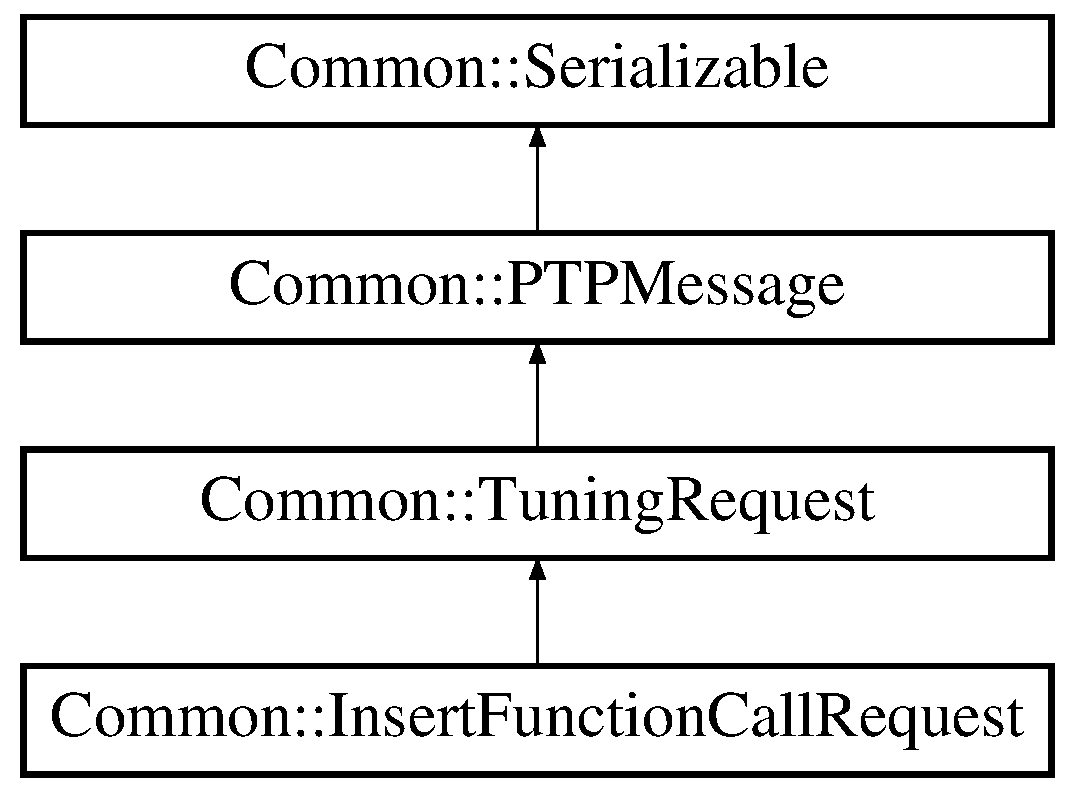
\includegraphics[height=4.000000cm]{class_common_1_1_insert_function_call_request}
\end{center}
\end{figure}
\subsection*{Public Member Functions}
\begin{DoxyCompactItemize}
\item 
\hyperlink{class_common_1_1_insert_function_call_request_afa5cae0e9adb14835c8afcca958454aa}{Insert\-Function\-Call\-Request} (int pid=0, std\-::string const \&func\-Name=std\-::string(), int n\-Attrs=0, \hyperlink{class_common_1_1_attribute}{Attribute} $\ast$attrs=0, std\-::string const \&dest\-Func=std\-::string(), Instr\-Place place=ip\-Func\-Entry, \hyperlink{class_common_1_1_breakpoint}{Breakpoint} $\ast$brkpt=0)
\begin{DoxyCompactList}\small\item\em Constructor. \end{DoxyCompactList}\item 
\hypertarget{class_common_1_1_insert_function_call_request_a0218e230b6e09b5cd8cba72940d716a7}{\hyperlink{class_common_1_1_insert_function_call_request_a0218e230b6e09b5cd8cba72940d716a7}{$\sim$\-Insert\-Function\-Call\-Request} ()}\label{class_common_1_1_insert_function_call_request_a0218e230b6e09b5cd8cba72940d716a7}

\begin{DoxyCompactList}\small\item\em Destructor. \end{DoxyCompactList}\item 
\hypertarget{class_common_1_1_insert_function_call_request_ab421754e776375ae71ffebec5489999d}{P\-T\-P\-Msg\-Type \hyperlink{class_common_1_1_insert_function_call_request_ab421754e776375ae71ffebec5489999d}{Get\-Type} () const }\label{class_common_1_1_insert_function_call_request_ab421754e776375ae71ffebec5489999d}

\begin{DoxyCompactList}\small\item\em Returns type of message (P\-T\-P\-Insert\-Func\-Call). \end{DoxyCompactList}\item 
\hypertarget{class_common_1_1_insert_function_call_request_a019fbc8dad4649cd2ead98062b7abd69}{std\-::string const \& \hyperlink{class_common_1_1_insert_function_call_request_a019fbc8dad4649cd2ead98062b7abd69}{Get\-Func\-Name} () const }\label{class_common_1_1_insert_function_call_request_a019fbc8dad4649cd2ead98062b7abd69}

\begin{DoxyCompactList}\small\item\em Returns name of the function to add. \end{DoxyCompactList}\item 
\hypertarget{class_common_1_1_insert_function_call_request_a1a23474cd80797817bb90e422f1b083f}{int \hyperlink{class_common_1_1_insert_function_call_request_a1a23474cd80797817bb90e422f1b083f}{Get\-Attr\-Count} () const }\label{class_common_1_1_insert_function_call_request_a1a23474cd80797817bb90e422f1b083f}

\begin{DoxyCompactList}\small\item\em Returns number of attributes the function has. \end{DoxyCompactList}\item 
\hypertarget{class_common_1_1_insert_function_call_request_aa74cefa1bcb949dafec52a1786be88ce}{\hyperlink{class_common_1_1_attribute}{Attribute} $\ast$ \hyperlink{class_common_1_1_insert_function_call_request_aa74cefa1bcb949dafec52a1786be88ce}{Get\-Attributes} () const }\label{class_common_1_1_insert_function_call_request_aa74cefa1bcb949dafec52a1786be88ce}

\begin{DoxyCompactList}\small\item\em Returns array of attributes. \end{DoxyCompactList}\item 
\hypertarget{class_common_1_1_insert_function_call_request_aa7bcff019a95a70e4c4e7816cc2e0050}{std\-::string const \& \hyperlink{class_common_1_1_insert_function_call_request_aa7bcff019a95a70e4c4e7816cc2e0050}{Get\-Dest\-Func} () const }\label{class_common_1_1_insert_function_call_request_aa7bcff019a95a70e4c4e7816cc2e0050}

\begin{DoxyCompactList}\small\item\em Returns name of the function where the call will be added. \end{DoxyCompactList}\item 
\hypertarget{class_common_1_1_insert_function_call_request_af1f4d5592bebe033b790c3bae1c801a0}{Instr\-Place \hyperlink{class_common_1_1_insert_function_call_request_af1f4d5592bebe033b790c3bae1c801a0}{Get\-Instr\-Place} () const }\label{class_common_1_1_insert_function_call_request_af1f4d5592bebe033b790c3bae1c801a0}

\begin{DoxyCompactList}\small\item\em Returns the place where the call will be added. \end{DoxyCompactList}\item 
\hypertarget{class_common_1_1_insert_function_call_request_af966bad75d6161fefd2683ff82504d74}{void \hyperlink{class_common_1_1_insert_function_call_request_af966bad75d6161fefd2683ff82504d74}{Serialize} (\hyperlink{class_common_1_1_serializer}{Serializer} \&out) const }\label{class_common_1_1_insert_function_call_request_af966bad75d6161fefd2683ff82504d74}

\begin{DoxyCompactList}\small\item\em Sends the message. \end{DoxyCompactList}\item 
\hypertarget{class_common_1_1_insert_function_call_request_a84571a179ad526574049a45066226171}{void \hyperlink{class_common_1_1_insert_function_call_request_a84571a179ad526574049a45066226171}{De\-Serialize} (\hyperlink{class_common_1_1_de_serializer}{De\-Serializer} \&in)}\label{class_common_1_1_insert_function_call_request_a84571a179ad526574049a45066226171}

\begin{DoxyCompactList}\small\item\em Receives the message. \end{DoxyCompactList}\end{DoxyCompactItemize}
\subsection*{Additional Inherited Members}


\subsection{Detailed Description}
Encapsulates a tuning request to insert a new function invocation code with a specified attributes at a given location in an application process. 

\begin{DoxyVersion}{Version}
1.\-0b 
\end{DoxyVersion}
\begin{DoxySince}{Since}
1.\-0b 
\end{DoxySince}
\begin{DoxyAuthor}{Author}
Ania Sikora, 2003 
\end{DoxyAuthor}


\subsection{Constructor \& Destructor Documentation}
\hypertarget{class_common_1_1_insert_function_call_request_afa5cae0e9adb14835c8afcca958454aa}{\index{Common\-::\-Insert\-Function\-Call\-Request@{Common\-::\-Insert\-Function\-Call\-Request}!Insert\-Function\-Call\-Request@{Insert\-Function\-Call\-Request}}
\index{Insert\-Function\-Call\-Request@{Insert\-Function\-Call\-Request}!Common::InsertFunctionCallRequest@{Common\-::\-Insert\-Function\-Call\-Request}}
\subsubsection[{Insert\-Function\-Call\-Request}]{\setlength{\rightskip}{0pt plus 5cm}Common\-::\-Insert\-Function\-Call\-Request\-::\-Insert\-Function\-Call\-Request (
\begin{DoxyParamCaption}
\item[{int}]{pid = {\ttfamily 0}, }
\item[{std\-::string const \&}]{func\-Name = {\ttfamily std\-:\-:string()}, }
\item[{int}]{n\-Attrs = {\ttfamily 0}, }
\item[{{\bf Attribute} $\ast$}]{attrs = {\ttfamily 0}, }
\item[{std\-::string const \&}]{dest\-Func = {\ttfamily std\-:\-:string()}, }
\item[{Instr\-Place}]{place = {\ttfamily ipFuncEntry}, }
\item[{{\bf Breakpoint} $\ast$}]{brkpt = {\ttfamily 0}}
\end{DoxyParamCaption}
)\hspace{0.3cm}{\ttfamily [inline]}}}\label{class_common_1_1_insert_function_call_request_afa5cae0e9adb14835c8afcca958454aa}


Constructor. 


\begin{DoxyParams}{Parameters}
{\em pid} & Id of the process where the call will be inserted, default 0. \\
\hline
{\em func\-Name} & Name of the function to call, default \char`\"{}\char`\"{}. \\
\hline
{\em n\-Attrs} & Number of attributes the function has, default 0. \\
\hline
{\em attrs} & \hyperlink{class_common_1_1_attribute}{Attribute} array, default 0. \\
\hline
{\em dest\-Func} & Function where the call will be inserted, default \char`\"{}\char`\"{}. \\
\hline
{\em place} & Place where the call will be added, default ip\-Func\-Entry. \\
\hline
{\em brkpt} & Used for synchronization purposes, the actual tuning will be executed when the execution reaches the breakpoint, default 0. \\
\hline
\end{DoxyParams}


The documentation for this class was generated from the following files\-:\begin{DoxyCompactItemize}
\item 
Common/P\-T\-P\-Msg.\-h\item 
Common/P\-T\-P\-Msg.\-cpp\end{DoxyCompactItemize}

\hypertarget{class_instr_group}{\section{Instr\-Group Class Reference}
\label{class_instr_group}\index{Instr\-Group@{Instr\-Group}}
}


Contains a group of snippets to be inserted in a function.  




{\ttfamily \#include $<$Instr\-Set.\-h$>$}

\subsection*{Public Types}
\begin{DoxyCompactItemize}
\item 
\hypertarget{class_instr_group_a4ef84ae062f916504d1cdd6f5f6437d7}{typedef vector$<$ \hyperlink{class_snippet_handler}{Snippet\-Handler} $\ast$ $>$\\*
\-::iterator {\bfseries Iterator}}\label{class_instr_group_a4ef84ae062f916504d1cdd6f5f6437d7}

\end{DoxyCompactItemize}
\subsection*{Public Member Functions}
\begin{DoxyCompactItemize}
\item 
\hypertarget{class_instr_group_a5e42e6a1eee81a9b67852cf9cba38703}{\hyperlink{class_instr_group_a5e42e6a1eee81a9b67852cf9cba38703}{Instr\-Group} (int event\-Id, std\-::string const \&func\-Name)}\label{class_instr_group_a5e42e6a1eee81a9b67852cf9cba38703}

\begin{DoxyCompactList}\small\item\em Constructor. \end{DoxyCompactList}\item 
\hypertarget{class_instr_group_a0a3d7f4dc0c35b8f254ff19badec2d3a}{\hyperlink{class_instr_group_a0a3d7f4dc0c35b8f254ff19badec2d3a}{$\sim$\-Instr\-Group} ()}\label{class_instr_group_a0a3d7f4dc0c35b8f254ff19badec2d3a}

\begin{DoxyCompactList}\small\item\em Destructor. \end{DoxyCompactList}\item 
int \hyperlink{class_instr_group_aa17d3fbb57017c6825fef8ea4a28deeb}{Get\-Event\-Id} () const 
\begin{DoxyCompactList}\small\item\em Getter for the variable \-\_\-event\-Id. \end{DoxyCompactList}\item 
int \hyperlink{class_instr_group_a86f2165483dfa146d662eb7d35f15e23}{Get\-Size} () const 
\begin{DoxyCompactList}\small\item\em Getter of the size of \-\_\-vector. \end{DoxyCompactList}\item 
bool \hyperlink{class_instr_group_ae58c61dd4ded42212e94e24dcc09133c}{Is\-Empty} () const 
\begin{DoxyCompactList}\small\item\em Checks if \-\_\-vector is empty. \end{DoxyCompactList}\item 
std\-::string const \& \hyperlink{class_instr_group_af563f5149b24343aed32dcc241d51861}{Get\-Func\-Name} () const 
\begin{DoxyCompactList}\small\item\em Getter of the name of the function. \end{DoxyCompactList}\item 
void \hyperlink{class_instr_group_addcd3f41da597eb9b1a8bab88d906c6c}{Add\-Handler} (Instr\-Place place, B\-Patch\-Snippet\-Handle $\ast$handle)
\begin{DoxyCompactList}\small\item\em Add the handler passed as a parameter to the \-\_\-vector. \end{DoxyCompactList}\item 
void \hyperlink{class_instr_group_aac2f0d8e6ae1d432634096016120f8dd}{Remove\-Handler} (Instr\-Place place)
\begin{DoxyCompactList}\small\item\em Eliminates the handlers from the vector to be inserted in the place passed as a parameter. \end{DoxyCompactList}\item 
Iterator \hyperlink{class_instr_group_a7397b4be484236b0e8a655a2a13abdc1}{begin} ()
\begin{DoxyCompactList}\small\item\em Getter for an iterator pointing to the first element in the \hyperlink{class_instr_group}{Instr\-Group}. \end{DoxyCompactList}\item 
Iterator \hyperlink{class_instr_group_ae975dcc604ba4d277d63e0889abb710d}{end} ()
\begin{DoxyCompactList}\small\item\em Getter for an iterator pointing to the last instruction (handler) on the group. \end{DoxyCompactList}\end{DoxyCompactItemize}


\subsection{Detailed Description}
Contains a group of snippets to be inserted in a function. 

\begin{DoxyVersion}{Version}
1.\-0 
\end{DoxyVersion}
\begin{DoxySince}{Since}
1.\-0 
\end{DoxySince}
\begin{DoxyAuthor}{Author}
Ania Sikora, 2002 
\end{DoxyAuthor}


\subsection{Member Function Documentation}
\hypertarget{class_instr_group_addcd3f41da597eb9b1a8bab88d906c6c}{\index{Instr\-Group@{Instr\-Group}!Add\-Handler@{Add\-Handler}}
\index{Add\-Handler@{Add\-Handler}!InstrGroup@{Instr\-Group}}
\subsubsection[{Add\-Handler}]{\setlength{\rightskip}{0pt plus 5cm}void Instr\-Group\-::\-Add\-Handler (
\begin{DoxyParamCaption}
\item[{Instr\-Place}]{place, }
\item[{B\-Patch\-Snippet\-Handle $\ast$}]{handle}
\end{DoxyParamCaption}
)}}\label{class_instr_group_addcd3f41da597eb9b1a8bab88d906c6c}


Add the handler passed as a parameter to the \-\_\-vector. 


\begin{DoxyParams}{Parameters}
{\em place} & Object that represents the place in the program in which the snippet will be inserted.\\
\hline
{\em handle} & Object of the class B\-Patch\-Snippet\-Handle that handles a Dyninst snippet. \\
\hline
\end{DoxyParams}
\hypertarget{class_instr_group_a7397b4be484236b0e8a655a2a13abdc1}{\index{Instr\-Group@{Instr\-Group}!begin@{begin}}
\index{begin@{begin}!InstrGroup@{Instr\-Group}}
\subsubsection[{begin}]{\setlength{\rightskip}{0pt plus 5cm}Iterator Instr\-Group\-::begin (
\begin{DoxyParamCaption}
{}
\end{DoxyParamCaption}
)\hspace{0.3cm}{\ttfamily [inline]}}}\label{class_instr_group_a7397b4be484236b0e8a655a2a13abdc1}


Getter for an iterator pointing to the first element in the \hyperlink{class_instr_group}{Instr\-Group}. 

\begin{DoxyReturn}{Returns}
Iterator for the variable \-\_\-vector that points to its beginning. 
\end{DoxyReturn}
\hypertarget{class_instr_group_ae975dcc604ba4d277d63e0889abb710d}{\index{Instr\-Group@{Instr\-Group}!end@{end}}
\index{end@{end}!InstrGroup@{Instr\-Group}}
\subsubsection[{end}]{\setlength{\rightskip}{0pt plus 5cm}Iterator Instr\-Group\-::end (
\begin{DoxyParamCaption}
{}
\end{DoxyParamCaption}
)\hspace{0.3cm}{\ttfamily [inline]}}}\label{class_instr_group_ae975dcc604ba4d277d63e0889abb710d}


Getter for an iterator pointing to the last instruction (handler) on the group. 

\begin{DoxyReturn}{Returns}
Iterator for the variable \-\_\-vector that points to its final element. 
\end{DoxyReturn}
\hypertarget{class_instr_group_aa17d3fbb57017c6825fef8ea4a28deeb}{\index{Instr\-Group@{Instr\-Group}!Get\-Event\-Id@{Get\-Event\-Id}}
\index{Get\-Event\-Id@{Get\-Event\-Id}!InstrGroup@{Instr\-Group}}
\subsubsection[{Get\-Event\-Id}]{\setlength{\rightskip}{0pt plus 5cm}int Instr\-Group\-::\-Get\-Event\-Id (
\begin{DoxyParamCaption}
{}
\end{DoxyParamCaption}
) const\hspace{0.3cm}{\ttfamily [inline]}}}\label{class_instr_group_aa17d3fbb57017c6825fef8ea4a28deeb}


Getter for the variable \-\_\-event\-Id. 

\begin{DoxyReturn}{Returns}
Id of the event. 
\end{DoxyReturn}
\hypertarget{class_instr_group_af563f5149b24343aed32dcc241d51861}{\index{Instr\-Group@{Instr\-Group}!Get\-Func\-Name@{Get\-Func\-Name}}
\index{Get\-Func\-Name@{Get\-Func\-Name}!InstrGroup@{Instr\-Group}}
\subsubsection[{Get\-Func\-Name}]{\setlength{\rightskip}{0pt plus 5cm}std\-::string const\& Instr\-Group\-::\-Get\-Func\-Name (
\begin{DoxyParamCaption}
{}
\end{DoxyParamCaption}
) const\hspace{0.3cm}{\ttfamily [inline]}}}\label{class_instr_group_af563f5149b24343aed32dcc241d51861}


Getter of the name of the function. 

\begin{DoxyReturn}{Returns}
String that contains the name of the function. 
\end{DoxyReturn}
\hypertarget{class_instr_group_a86f2165483dfa146d662eb7d35f15e23}{\index{Instr\-Group@{Instr\-Group}!Get\-Size@{Get\-Size}}
\index{Get\-Size@{Get\-Size}!InstrGroup@{Instr\-Group}}
\subsubsection[{Get\-Size}]{\setlength{\rightskip}{0pt plus 5cm}int Instr\-Group\-::\-Get\-Size (
\begin{DoxyParamCaption}
{}
\end{DoxyParamCaption}
) const\hspace{0.3cm}{\ttfamily [inline]}}}\label{class_instr_group_a86f2165483dfa146d662eb7d35f15e23}


Getter of the size of \-\_\-vector. 

\begin{DoxyReturn}{Returns}
Size of the vector \-\_\-vector. 
\end{DoxyReturn}
\hypertarget{class_instr_group_ae58c61dd4ded42212e94e24dcc09133c}{\index{Instr\-Group@{Instr\-Group}!Is\-Empty@{Is\-Empty}}
\index{Is\-Empty@{Is\-Empty}!InstrGroup@{Instr\-Group}}
\subsubsection[{Is\-Empty}]{\setlength{\rightskip}{0pt plus 5cm}bool Instr\-Group\-::\-Is\-Empty (
\begin{DoxyParamCaption}
{}
\end{DoxyParamCaption}
) const\hspace{0.3cm}{\ttfamily [inline]}}}\label{class_instr_group_ae58c61dd4ded42212e94e24dcc09133c}


Checks if \-\_\-vector is empty. 

\begin{DoxyReturn}{Returns}
0 if not empty, 1 if empty. 
\end{DoxyReturn}
\hypertarget{class_instr_group_aac2f0d8e6ae1d432634096016120f8dd}{\index{Instr\-Group@{Instr\-Group}!Remove\-Handler@{Remove\-Handler}}
\index{Remove\-Handler@{Remove\-Handler}!InstrGroup@{Instr\-Group}}
\subsubsection[{Remove\-Handler}]{\setlength{\rightskip}{0pt plus 5cm}void Instr\-Group\-::\-Remove\-Handler (
\begin{DoxyParamCaption}
\item[{Instr\-Place}]{place}
\end{DoxyParamCaption}
)}}\label{class_instr_group_aac2f0d8e6ae1d432634096016120f8dd}


Eliminates the handlers from the vector to be inserted in the place passed as a parameter. 


\begin{DoxyParams}{Parameters}
{\em place} & Object that represents the place in the program in which the snippet will be inserted. \\
\hline
\end{DoxyParams}


The documentation for this class was generated from the following files\-:\begin{DoxyCompactItemize}
\item 
A\-C/Instr\-Set.\-h\item 
A\-C/Instr\-Set.\-cpp\end{DoxyCompactItemize}

\hypertarget{class_common_1_1_config_map_1_1_iterator}{\section{Common\-:\-:Config\-Map\-:\-:Iterator Class Reference}
\label{class_common_1_1_config_map_1_1_iterator}\index{Common\-::\-Config\-Map\-::\-Iterator@{Common\-::\-Config\-Map\-::\-Iterator}}
}


Iterates over a \hyperlink{class_common_1_1_config_map}{Config\-Map} object.  




{\ttfamily \#include $<$Config\-Map.\-h$>$}

\subsection*{Public Member Functions}
\begin{DoxyCompactItemize}
\item 
\hypertarget{class_common_1_1_config_map_1_1_iterator_acfa68189c1818ee0f96ab71213fdd2e4}{\hyperlink{class_common_1_1_config_map_1_1_iterator_acfa68189c1818ee0f96ab71213fdd2e4}{Iterator} (\hyperlink{class_common_1_1_config_map}{Config\-Map} const \&map)}\label{class_common_1_1_config_map_1_1_iterator_acfa68189c1818ee0f96ab71213fdd2e4}

\begin{DoxyCompactList}\small\item\em Constructor. \end{DoxyCompactList}\item 
\hypertarget{class_common_1_1_config_map_1_1_iterator_a94b26142475c2eac71a2e2c3fad4f590}{bool \hyperlink{class_common_1_1_config_map_1_1_iterator_a94b26142475c2eac71a2e2c3fad4f590}{At\-End} () const }\label{class_common_1_1_config_map_1_1_iterator_a94b26142475c2eac71a2e2c3fad4f590}

\begin{DoxyCompactList}\small\item\em Indicates whether the iterator is pointing to the end of the map or not. \end{DoxyCompactList}\item 
\hypertarget{class_common_1_1_config_map_1_1_iterator_a69195c2f4220631fe0a772007ed30ca6}{void \hyperlink{class_common_1_1_config_map_1_1_iterator_a69195c2f4220631fe0a772007ed30ca6}{Next} ()}\label{class_common_1_1_config_map_1_1_iterator_a69195c2f4220631fe0a772007ed30ca6}

\begin{DoxyCompactList}\small\item\em The pointer increases a position on the map. \end{DoxyCompactList}\item 
\hypertarget{class_common_1_1_config_map_1_1_iterator_a4cdec86d82eab91cf1c5f8f59f3e2f70}{std\-::string \hyperlink{class_common_1_1_config_map_1_1_iterator_a4cdec86d82eab91cf1c5f8f59f3e2f70}{Get\-Section} () const }\label{class_common_1_1_config_map_1_1_iterator_a4cdec86d82eab91cf1c5f8f59f3e2f70}

\begin{DoxyCompactList}\small\item\em Returns section of the current position. \end{DoxyCompactList}\item 
\hypertarget{class_common_1_1_config_map_1_1_iterator_a67d5501f3b15143986f02864787cf710}{std\-::string \hyperlink{class_common_1_1_config_map_1_1_iterator_a67d5501f3b15143986f02864787cf710}{Get\-Key} () const }\label{class_common_1_1_config_map_1_1_iterator_a67d5501f3b15143986f02864787cf710}

\begin{DoxyCompactList}\small\item\em Returns key of the current position. \end{DoxyCompactList}\item 
\hypertarget{class_common_1_1_config_map_1_1_iterator_aff11c0a07605df50c48e300de7fd05e6}{std\-::string const \& \hyperlink{class_common_1_1_config_map_1_1_iterator_aff11c0a07605df50c48e300de7fd05e6}{Get\-Value} () const }\label{class_common_1_1_config_map_1_1_iterator_aff11c0a07605df50c48e300de7fd05e6}

\begin{DoxyCompactList}\small\item\em Returns value of the current position. \end{DoxyCompactList}\end{DoxyCompactItemize}


\subsection{Detailed Description}
Iterates over a \hyperlink{class_common_1_1_config_map}{Config\-Map} object. 

\begin{DoxyVersion}{Version}
1.\-0b 
\end{DoxyVersion}
\begin{DoxySince}{Since}
1.\-0b 
\end{DoxySince}
\begin{DoxyAuthor}{Author}
Ania Sikora, 2000 
\end{DoxyAuthor}


The documentation for this class was generated from the following files\-:\begin{DoxyCompactItemize}
\item 
Common/Config\-Map.\-h\item 
Common/Config\-Map.\-cpp\end{DoxyCompactItemize}

\hypertarget{class_iter_data}{\section{Iter\-Data Class Reference}
\label{class_iter_data}\index{Iter\-Data@{Iter\-Data}}
}


Statistics for a single iteration.  




{\ttfamily \#include $<$Factoring\-Stats\-\_\-nw.\-h$>$}

\subsection*{Public Member Functions}
\begin{DoxyCompactItemize}
\item 
\hyperlink{class_iter_data_afec41827476662cb1cac6d0f00931a80}{Iter\-Data} (int iter\-Idx)
\begin{DoxyCompactList}\small\item\em Constructor. \end{DoxyCompactList}\item 
\hypertarget{class_iter_data_a14ebf5f539d8941043b026513908f281}{\hyperlink{class_iter_data_a14ebf5f539d8941043b026513908f281}{$\sim$\-Iter\-Data} ()}\label{class_iter_data_a14ebf5f539d8941043b026513908f281}

\begin{DoxyCompactList}\small\item\em Destructor. \end{DoxyCompactList}\item 
void \hyperlink{class_iter_data_ab6cc53385450be8716cae65eebb7757e}{On\-Iter\-Start} (long\-\_\-t time, int num\-Tuples, int size\-Bytes, int nw)
\begin{DoxyCompactList}\small\item\em Sets the flag of the iteration started to 1, the iteration starting time to {\itshape time}, the number of tasks as {\itshape num\-Tuples}, the number of workers to {\itshape nw} and the size in Bytes to {\itshape size\-Bytes}. \end{DoxyCompactList}\item 
void \hyperlink{class_iter_data_a4043a0cbd3de9f8e7e4b3438b6b861b2}{On\-Iter\-End} (long\-\_\-t time)
\begin{DoxyCompactList}\small\item\em Sets the flag of the finishing iteration to 1 and makes sure that the final time stated in {\itshape time} is greater than the starting one. Finally, it computes the iteration's elapsed time. \end{DoxyCompactList}\item 
\hypertarget{class_iter_data_ad771031edb8d8dfa35691bba78b94fd7}{void \hyperlink{class_iter_data_ad771031edb8d8dfa35691bba78b94fd7}{On\-New\-Batch} ()}\label{class_iter_data_ad771031edb8d8dfa35691bba78b94fd7}

\begin{DoxyCompactList}\small\item\em Increments the number of batches by 1. \end{DoxyCompactList}\item 
\hyperlink{class_batch_data}{Batch\-Data} \& \hyperlink{class_iter_data_ac437f6f1b288d95d07a341420985d560}{Get\-Batch\-Data} (int Idx\-Batch)
\begin{DoxyCompactList}\small\item\em Gets the data in a batch by specifying the batch I\-D. If it's the last node from the iterator, adds a new \hyperlink{class_batch_data}{Batch\-Data} object and returns it. \end{DoxyCompactList}\item 
bool \hyperlink{class_iter_data_af2ae93caf86c95f45c505846a698b9e2}{Is\-Complete} () const 
\begin{DoxyCompactList}\small\item\em Checks if the current iteration has a start and an end and whether all batches are complete. \end{DoxyCompactList}\item 
bool \hyperlink{class_iter_data_a26f9b64165ba90f882aa7ca4e0896cc3}{Are\-Batchs\-Complete} () const 
\begin{DoxyCompactList}\small\item\em Checks if all batches are complete. \end{DoxyCompactList}\item 
int \hyperlink{class_iter_data_a41a194699551536e6a32b9558edee861}{Get\-Tuple\-Size\-In\-Bytes} () const 
\begin{DoxyCompactList}\small\item\em Getter of the tuple size in bytes. \end{DoxyCompactList}\item 
\hyperlink{class_batch_data}{Batch\-Data} $\ast$$\ast$ \hyperlink{class_iter_data_a027f9296d3a93d9e5b15abc08519acfc}{Alloc\-Batchs\-Array} ()
\begin{DoxyCompactList}\small\item\em Allocates a new batch data for each element in the array \-\_\-map\-B. \end{DoxyCompactList}\item 
int \hyperlink{class_iter_data_a77586ae939bcca9bbbedf71bc692da89}{Get\-Num\-Workers} ()
\begin{DoxyCompactList}\small\item\em Getter of the number of workers. \end{DoxyCompactList}\item 
int \hyperlink{class_iter_data_ab2bf30bbc572a350ca4a492adc0f6bf9}{Get\-Total\-Tasks} () const 
\begin{DoxyCompactList}\small\item\em Getter of the number of tasks. \end{DoxyCompactList}\item 
int \hyperlink{class_iter_data_acd80b709571a608eca0af0145c4ad684}{Get\-Num\-Batchs} () const 
\begin{DoxyCompactList}\small\item\em Getter of the number of batches. \end{DoxyCompactList}\end{DoxyCompactItemize}


\subsection{Detailed Description}
Statistics for a single iteration. 

\subsection{Constructor \& Destructor Documentation}
\hypertarget{class_iter_data_afec41827476662cb1cac6d0f00931a80}{\index{Iter\-Data@{Iter\-Data}!Iter\-Data@{Iter\-Data}}
\index{Iter\-Data@{Iter\-Data}!IterData@{Iter\-Data}}
\subsubsection[{Iter\-Data}]{\setlength{\rightskip}{0pt plus 5cm}Iter\-Data\-::\-Iter\-Data (
\begin{DoxyParamCaption}
\item[{int}]{iter\-Idx}
\end{DoxyParamCaption}
)}}\label{class_iter_data_afec41827476662cb1cac6d0f00931a80}


Constructor. 


\begin{DoxyParams}{Parameters}
{\em iter\-Idx} & I\-D of the iterator \\
\hline
\end{DoxyParams}


\subsection{Member Function Documentation}
\hypertarget{class_iter_data_a027f9296d3a93d9e5b15abc08519acfc}{\index{Iter\-Data@{Iter\-Data}!Alloc\-Batchs\-Array@{Alloc\-Batchs\-Array}}
\index{Alloc\-Batchs\-Array@{Alloc\-Batchs\-Array}!IterData@{Iter\-Data}}
\subsubsection[{Alloc\-Batchs\-Array}]{\setlength{\rightskip}{0pt plus 5cm}{\bf Batch\-Data} $\ast$$\ast$ Iter\-Data\-::\-Alloc\-Batchs\-Array (
\begin{DoxyParamCaption}
{}
\end{DoxyParamCaption}
)}}\label{class_iter_data_a027f9296d3a93d9e5b15abc08519acfc}


Allocates a new batch data for each element in the array \-\_\-map\-B. 

\begin{DoxyReturn}{Returns}
Array with all batches allocated 
\end{DoxyReturn}
\hypertarget{class_iter_data_a26f9b64165ba90f882aa7ca4e0896cc3}{\index{Iter\-Data@{Iter\-Data}!Are\-Batchs\-Complete@{Are\-Batchs\-Complete}}
\index{Are\-Batchs\-Complete@{Are\-Batchs\-Complete}!IterData@{Iter\-Data}}
\subsubsection[{Are\-Batchs\-Complete}]{\setlength{\rightskip}{0pt plus 5cm}bool Iter\-Data\-::\-Are\-Batchs\-Complete (
\begin{DoxyParamCaption}
{}
\end{DoxyParamCaption}
) const}}\label{class_iter_data_a26f9b64165ba90f882aa7ca4e0896cc3}


Checks if all batches are complete. 

\begin{DoxyReturn}{Returns}
True if all batches are complete and False if not. 
\end{DoxyReturn}
\hypertarget{class_iter_data_ac437f6f1b288d95d07a341420985d560}{\index{Iter\-Data@{Iter\-Data}!Get\-Batch\-Data@{Get\-Batch\-Data}}
\index{Get\-Batch\-Data@{Get\-Batch\-Data}!IterData@{Iter\-Data}}
\subsubsection[{Get\-Batch\-Data}]{\setlength{\rightskip}{0pt plus 5cm}{\bf Batch\-Data} \& Iter\-Data\-::\-Get\-Batch\-Data (
\begin{DoxyParamCaption}
\item[{int}]{Idx\-Batch}
\end{DoxyParamCaption}
)}}\label{class_iter_data_ac437f6f1b288d95d07a341420985d560}


Gets the data in a batch by specifying the batch I\-D. If it's the last node from the iterator, adds a new \hyperlink{class_batch_data}{Batch\-Data} object and returns it. 


\begin{DoxyParams}{Parameters}
{\em Idx\-Batch} & \\
\hline
\end{DoxyParams}
\begin{DoxyReturn}{Returns}
Data of the batch in a \hyperlink{class_batch_data}{Batch\-Data} object 
\end{DoxyReturn}
\hypertarget{class_iter_data_acd80b709571a608eca0af0145c4ad684}{\index{Iter\-Data@{Iter\-Data}!Get\-Num\-Batchs@{Get\-Num\-Batchs}}
\index{Get\-Num\-Batchs@{Get\-Num\-Batchs}!IterData@{Iter\-Data}}
\subsubsection[{Get\-Num\-Batchs}]{\setlength{\rightskip}{0pt plus 5cm}int Iter\-Data\-::\-Get\-Num\-Batchs (
\begin{DoxyParamCaption}
{}
\end{DoxyParamCaption}
) const\hspace{0.3cm}{\ttfamily [inline]}}}\label{class_iter_data_acd80b709571a608eca0af0145c4ad684}


Getter of the number of batches. 

\begin{DoxyReturn}{Returns}
\-\_\-nbatchs 
\end{DoxyReturn}
\hypertarget{class_iter_data_a77586ae939bcca9bbbedf71bc692da89}{\index{Iter\-Data@{Iter\-Data}!Get\-Num\-Workers@{Get\-Num\-Workers}}
\index{Get\-Num\-Workers@{Get\-Num\-Workers}!IterData@{Iter\-Data}}
\subsubsection[{Get\-Num\-Workers}]{\setlength{\rightskip}{0pt plus 5cm}int Iter\-Data\-::\-Get\-Num\-Workers (
\begin{DoxyParamCaption}
{}
\end{DoxyParamCaption}
)\hspace{0.3cm}{\ttfamily [inline]}}}\label{class_iter_data_a77586ae939bcca9bbbedf71bc692da89}


Getter of the number of workers. 

\begin{DoxyReturn}{Returns}
\-\_\-num\-Workers 
\end{DoxyReturn}
\hypertarget{class_iter_data_ab2bf30bbc572a350ca4a492adc0f6bf9}{\index{Iter\-Data@{Iter\-Data}!Get\-Total\-Tasks@{Get\-Total\-Tasks}}
\index{Get\-Total\-Tasks@{Get\-Total\-Tasks}!IterData@{Iter\-Data}}
\subsubsection[{Get\-Total\-Tasks}]{\setlength{\rightskip}{0pt plus 5cm}int Iter\-Data\-::\-Get\-Total\-Tasks (
\begin{DoxyParamCaption}
{}
\end{DoxyParamCaption}
) const\hspace{0.3cm}{\ttfamily [inline]}}}\label{class_iter_data_ab2bf30bbc572a350ca4a492adc0f6bf9}


Getter of the number of tasks. 

\begin{DoxyReturn}{Returns}
\-\_\-num\-Tasks 
\end{DoxyReturn}
\hypertarget{class_iter_data_a41a194699551536e6a32b9558edee861}{\index{Iter\-Data@{Iter\-Data}!Get\-Tuple\-Size\-In\-Bytes@{Get\-Tuple\-Size\-In\-Bytes}}
\index{Get\-Tuple\-Size\-In\-Bytes@{Get\-Tuple\-Size\-In\-Bytes}!IterData@{Iter\-Data}}
\subsubsection[{Get\-Tuple\-Size\-In\-Bytes}]{\setlength{\rightskip}{0pt plus 5cm}int Iter\-Data\-::\-Get\-Tuple\-Size\-In\-Bytes (
\begin{DoxyParamCaption}
{}
\end{DoxyParamCaption}
) const\hspace{0.3cm}{\ttfamily [inline]}}}\label{class_iter_data_a41a194699551536e6a32b9558edee861}


Getter of the tuple size in bytes. 

\begin{DoxyReturn}{Returns}
\-\_\-size\-Bytes 
\end{DoxyReturn}
\hypertarget{class_iter_data_af2ae93caf86c95f45c505846a698b9e2}{\index{Iter\-Data@{Iter\-Data}!Is\-Complete@{Is\-Complete}}
\index{Is\-Complete@{Is\-Complete}!IterData@{Iter\-Data}}
\subsubsection[{Is\-Complete}]{\setlength{\rightskip}{0pt plus 5cm}bool Iter\-Data\-::\-Is\-Complete (
\begin{DoxyParamCaption}
{}
\end{DoxyParamCaption}
) const\hspace{0.3cm}{\ttfamily [inline]}}}\label{class_iter_data_af2ae93caf86c95f45c505846a698b9e2}


Checks if the current iteration has a start and an end and whether all batches are complete. 

\begin{DoxyReturn}{Returns}
True if the current iteration is complete or False if not 
\end{DoxyReturn}
\hypertarget{class_iter_data_a4043a0cbd3de9f8e7e4b3438b6b861b2}{\index{Iter\-Data@{Iter\-Data}!On\-Iter\-End@{On\-Iter\-End}}
\index{On\-Iter\-End@{On\-Iter\-End}!IterData@{Iter\-Data}}
\subsubsection[{On\-Iter\-End}]{\setlength{\rightskip}{0pt plus 5cm}void Iter\-Data\-::\-On\-Iter\-End (
\begin{DoxyParamCaption}
\item[{long\-\_\-t}]{time}
\end{DoxyParamCaption}
)}}\label{class_iter_data_a4043a0cbd3de9f8e7e4b3438b6b861b2}


Sets the flag of the finishing iteration to 1 and makes sure that the final time stated in {\itshape time} is greater than the starting one. Finally, it computes the iteration's elapsed time. 


\begin{DoxyParams}{Parameters}
{\em time} & Ending time of the iteration. \\
\hline
\end{DoxyParams}
\hypertarget{class_iter_data_ab6cc53385450be8716cae65eebb7757e}{\index{Iter\-Data@{Iter\-Data}!On\-Iter\-Start@{On\-Iter\-Start}}
\index{On\-Iter\-Start@{On\-Iter\-Start}!IterData@{Iter\-Data}}
\subsubsection[{On\-Iter\-Start}]{\setlength{\rightskip}{0pt plus 5cm}void Iter\-Data\-::\-On\-Iter\-Start (
\begin{DoxyParamCaption}
\item[{long\-\_\-t}]{time, }
\item[{int}]{num\-Tuples, }
\item[{int}]{size\-Bytes, }
\item[{int}]{nw}
\end{DoxyParamCaption}
)}}\label{class_iter_data_ab6cc53385450be8716cae65eebb7757e}


Sets the flag of the iteration started to 1, the iteration starting time to {\itshape time}, the number of tasks as {\itshape num\-Tuples}, the number of workers to {\itshape nw} and the size in Bytes to {\itshape size\-Bytes}. 


\begin{DoxyParams}{Parameters}
{\em time} & Starting time of the iteration in milliseconds \\
\hline
{\em num\-Tuples} & Number of tasks \\
\hline
{\em size\-Bytes} & \hyperlink{class_task}{Task} size in Bytes \\
\hline
{\em nw} & Number of workers \\
\hline
\end{DoxyParams}


The documentation for this class was generated from the following files\-:\begin{DoxyCompactItemize}
\item 
Analyzer/Factoring\-Stats\-\_\-nw.\-h\item 
Analyzer/Factoring\-Stats\-\_\-nw.\-cpp\end{DoxyCompactItemize}

\hypertarget{class_common_1_1_config_1_1_key_iterator}{\section{Common\-:\-:Config\-:\-:Key\-Iterator Class Reference}
\label{class_common_1_1_config_1_1_key_iterator}\index{Common\-::\-Config\-::\-Key\-Iterator@{Common\-::\-Config\-::\-Key\-Iterator}}
}


Iterates over the keys of a \hyperlink{class_common_1_1_config}{Config} object.  




{\ttfamily \#include $<$Config.\-h$>$}

\subsection*{Public Member Functions}
\begin{DoxyCompactItemize}
\item 
\hypertarget{class_common_1_1_config_1_1_key_iterator_adaa4d99e98bfb25671086c090b079c23}{\hyperlink{class_common_1_1_config_1_1_key_iterator_adaa4d99e98bfb25671086c090b079c23}{Key\-Iterator} (\hyperlink{class_common_1_1_config}{Config} const \&config, std\-::string const \&section)}\label{class_common_1_1_config_1_1_key_iterator_adaa4d99e98bfb25671086c090b079c23}

\begin{DoxyCompactList}\small\item\em Constructor. \end{DoxyCompactList}\item 
\hypertarget{class_common_1_1_config_1_1_key_iterator_af24a3e94fd55dd118341ea681316357e}{bool \hyperlink{class_common_1_1_config_1_1_key_iterator_af24a3e94fd55dd118341ea681316357e}{At\-End} () const }\label{class_common_1_1_config_1_1_key_iterator_af24a3e94fd55dd118341ea681316357e}

\begin{DoxyCompactList}\small\item\em Indicates whether the iterator is pointing to the end of the map or not. \end{DoxyCompactList}\item 
\hypertarget{class_common_1_1_config_1_1_key_iterator_ae5db94c2dcb6af8eaca90d9d0dd4817b}{void \hyperlink{class_common_1_1_config_1_1_key_iterator_ae5db94c2dcb6af8eaca90d9d0dd4817b}{Next} ()}\label{class_common_1_1_config_1_1_key_iterator_ae5db94c2dcb6af8eaca90d9d0dd4817b}

\begin{DoxyCompactList}\small\item\em The pointer increases a position on the config. \end{DoxyCompactList}\item 
\hypertarget{class_common_1_1_config_1_1_key_iterator_a06d9d0caa42ec6ed9f3aa893b2292c7f}{std\-::string \hyperlink{class_common_1_1_config_1_1_key_iterator_a06d9d0caa42ec6ed9f3aa893b2292c7f}{Get\-Key} () const }\label{class_common_1_1_config_1_1_key_iterator_a06d9d0caa42ec6ed9f3aa893b2292c7f}

\begin{DoxyCompactList}\small\item\em Returns key of the current position. \end{DoxyCompactList}\item 
\hypertarget{class_common_1_1_config_1_1_key_iterator_aab4a93ab882fa45a803d9bc55203f071}{std\-::string const \& \hyperlink{class_common_1_1_config_1_1_key_iterator_aab4a93ab882fa45a803d9bc55203f071}{Get\-Value} () const }\label{class_common_1_1_config_1_1_key_iterator_aab4a93ab882fa45a803d9bc55203f071}

\begin{DoxyCompactList}\small\item\em Returns value of the current position. \end{DoxyCompactList}\item 
\hypertarget{class_common_1_1_config_1_1_key_iterator_a3a148b7ae0989eebcd68e9f49490b335}{int \hyperlink{class_common_1_1_config_1_1_key_iterator_a3a148b7ae0989eebcd68e9f49490b335}{Get\-Int\-Value} () const }\label{class_common_1_1_config_1_1_key_iterator_a3a148b7ae0989eebcd68e9f49490b335}

\begin{DoxyCompactList}\small\item\em Returns integer value of the current position. \end{DoxyCompactList}\end{DoxyCompactItemize}


\subsection{Detailed Description}
Iterates over the keys of a \hyperlink{class_common_1_1_config}{Config} object. 

\begin{DoxyVersion}{Version}
1.\-0b 
\end{DoxyVersion}
\begin{DoxySince}{Since}
1.\-0b 
\end{DoxySince}
\begin{DoxyAuthor}{Author}
Ania Sikora, 2000 
\end{DoxyAuthor}


The documentation for this class was generated from the following files\-:\begin{DoxyCompactItemize}
\item 
Common/Config.\-h\item 
Common/Config.\-cpp\end{DoxyCompactItemize}

\hypertarget{class_common_1_1_load_library_request}{\section{Common\-:\-:Load\-Library\-Request Class Reference}
\label{class_common_1_1_load_library_request}\index{Common\-::\-Load\-Library\-Request@{Common\-::\-Load\-Library\-Request}}
}


Encapsulates a tuning request to load the specified shared library to a given application process.  




{\ttfamily \#include $<$P\-T\-P\-Msg.\-h$>$}

Inheritance diagram for Common\-:\-:Load\-Library\-Request\-:\begin{figure}[H]
\begin{center}
\leavevmode
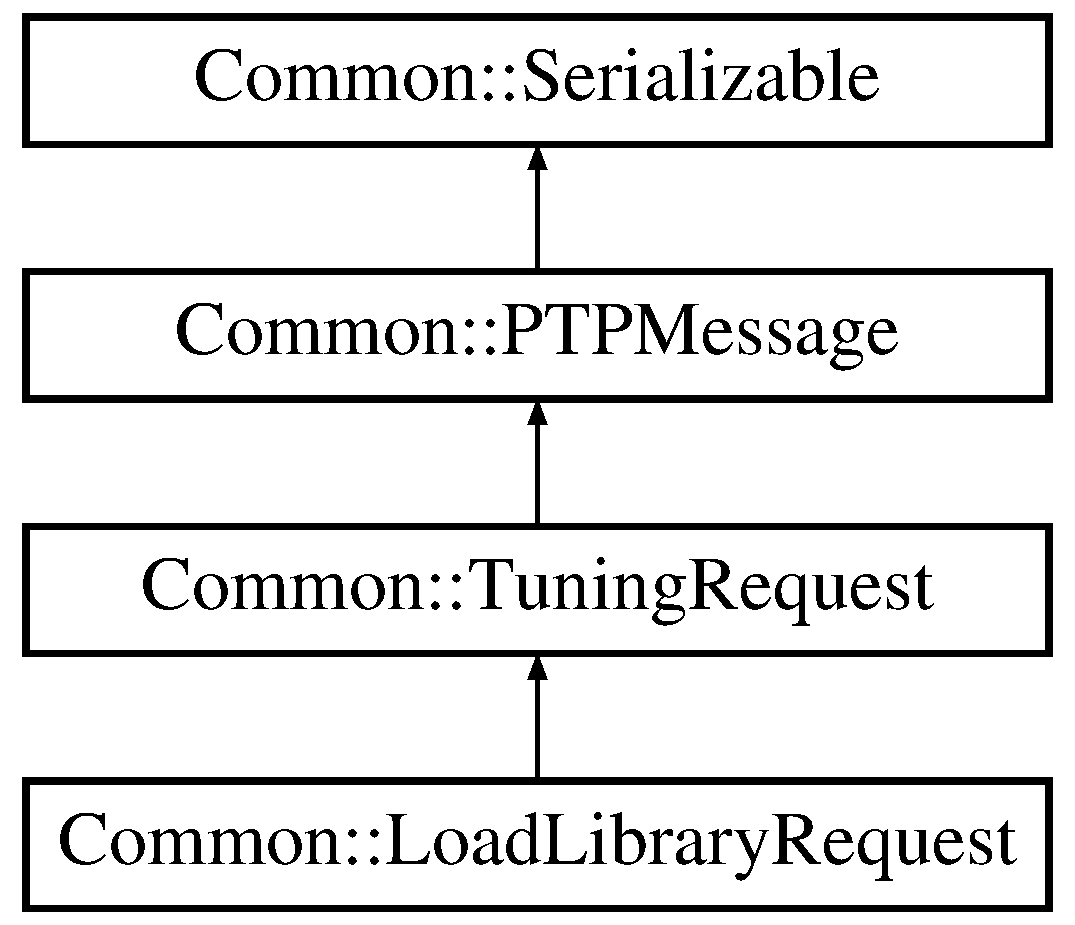
\includegraphics[height=4.000000cm]{class_common_1_1_load_library_request}
\end{center}
\end{figure}
\subsection*{Public Member Functions}
\begin{DoxyCompactItemize}
\item 
\hypertarget{class_common_1_1_load_library_request_adbd885a623010c20256b12a74ab7d2f6}{{\bfseries \-\_\-lib\-Path} (lib\-Path)}\label{class_common_1_1_load_library_request_adbd885a623010c20256b12a74ab7d2f6}

\item 
\hypertarget{class_common_1_1_load_library_request_a21fad1cc9656d8dd33134f384e10b8ea}{P\-T\-P\-Msg\-Type \hyperlink{class_common_1_1_load_library_request_a21fad1cc9656d8dd33134f384e10b8ea}{Get\-Type} () const }\label{class_common_1_1_load_library_request_a21fad1cc9656d8dd33134f384e10b8ea}

\begin{DoxyCompactList}\small\item\em Returns type of message (P\-T\-P\-Load\-Library). \end{DoxyCompactList}\item 
\hypertarget{class_common_1_1_load_library_request_af489b1ea9db673544f194f2e33ee9208}{std\-::string const \& \hyperlink{class_common_1_1_load_library_request_af489b1ea9db673544f194f2e33ee9208}{Get\-Library\-Path} () const }\label{class_common_1_1_load_library_request_af489b1ea9db673544f194f2e33ee9208}

\begin{DoxyCompactList}\small\item\em Returns the path of the library to be loaded. \end{DoxyCompactList}\item 
\hypertarget{class_common_1_1_load_library_request_a6be57195377b5077b9e551ba14da8721}{void \hyperlink{class_common_1_1_load_library_request_a6be57195377b5077b9e551ba14da8721}{Serialize} (\hyperlink{class_common_1_1_serializer}{Serializer} \&out) const }\label{class_common_1_1_load_library_request_a6be57195377b5077b9e551ba14da8721}

\begin{DoxyCompactList}\small\item\em Sends the message. \end{DoxyCompactList}\item 
\hypertarget{class_common_1_1_load_library_request_ae61c03221c7a69f6abaf133fd62fafe5}{void \hyperlink{class_common_1_1_load_library_request_ae61c03221c7a69f6abaf133fd62fafe5}{De\-Serialize} (\hyperlink{class_common_1_1_de_serializer}{De\-Serializer} \&in)}\label{class_common_1_1_load_library_request_ae61c03221c7a69f6abaf133fd62fafe5}

\begin{DoxyCompactList}\small\item\em Receives the message. \end{DoxyCompactList}\end{DoxyCompactItemize}
\subsection*{Public Attributes}
\begin{DoxyCompactItemize}
\item 
\hyperlink{class_common_1_1_load_library_request_a978d8b62146b28487b00bd0394aa3c12}{\-\_\-\-\_\-pad0\-\_\-\-\_\-}\-: \hyperlink{class_common_1_1_tuning_request}{Tuning\-Request} (pid
\begin{DoxyCompactList}\small\item\em Constructor. \end{DoxyCompactList}\end{DoxyCompactItemize}
\subsection*{Additional Inherited Members}


\subsection{Detailed Description}
Encapsulates a tuning request to load the specified shared library to a given application process. 

\begin{DoxyVersion}{Version}
1.\-0b 
\end{DoxyVersion}
\begin{DoxySince}{Since}
1.\-0b 
\end{DoxySince}
\begin{DoxyAuthor}{Author}
Ania Sikora, 2003 
\end{DoxyAuthor}


\subsection{Member Data Documentation}
\hypertarget{class_common_1_1_load_library_request_a978d8b62146b28487b00bd0394aa3c12}{\index{Common\-::\-Load\-Library\-Request@{Common\-::\-Load\-Library\-Request}!\-\_\-\-\_\-pad0\-\_\-\-\_\-@{\-\_\-\-\_\-pad0\-\_\-\-\_\-}}
\index{\-\_\-\-\_\-pad0\-\_\-\-\_\-@{\-\_\-\-\_\-pad0\-\_\-\-\_\-}!Common::LoadLibraryRequest@{Common\-::\-Load\-Library\-Request}}
\subsubsection[{\-\_\-\-\_\-pad0\-\_\-\-\_\-}]{\setlength{\rightskip}{0pt plus 5cm}Common\-::\-Load\-Library\-Request\-::\-\_\-\-\_\-pad0\-\_\-\-\_\-}}\label{class_common_1_1_load_library_request_a978d8b62146b28487b00bd0394aa3c12}


Constructor. 


\begin{DoxyParams}{Parameters}
{\em pid} & Id of the process where the library will be included, default 0. \\
\hline
{\em lib\-Path} & Path of the library, default \char`\"{}\char`\"{}. \\
\hline
\end{DoxyParams}


The documentation for this class was generated from the following files\-:\begin{DoxyCompactItemize}
\item 
Common/P\-T\-P\-Msg.\-h\item 
Common/P\-T\-P\-Msg.\-cpp\end{DoxyCompactItemize}

\hypertarget{class_common_1_1_log_entry}{\section{Common\-:\-:Log\-Entry Class Reference}
\label{class_common_1_1_log_entry}\index{Common\-::\-Log\-Entry@{Common\-::\-Log\-Entry}}
}


Entry on a log.  




{\ttfamily \#include $<$Syslog.\-h$>$}

\subsection*{Public Member Functions}
\begin{DoxyCompactItemize}
\item 
\hyperlink{class_common_1_1_log_entry_aea7d9e006bce770b70a2016b166facf7}{Log\-Entry} (Log\-Severity s, std\-::string const \&message)
\begin{DoxyCompactList}\small\item\em Constructor. \end{DoxyCompactList}\item 
\hypertarget{class_common_1_1_log_entry_a25542669cbc352a384874c30ca36d3e2}{\hyperlink{class_common_1_1_date_time}{Date\-Time} const \& \hyperlink{class_common_1_1_log_entry_a25542669cbc352a384874c30ca36d3e2}{Get\-Timestamp} () const }\label{class_common_1_1_log_entry_a25542669cbc352a384874c30ca36d3e2}

\begin{DoxyCompactList}\small\item\em Returns the date when the entry was performed. \end{DoxyCompactList}\item 
Log\-Severity \hyperlink{class_common_1_1_log_entry_a7a86f1c5e30447a395c0c070e76dcfcb}{Get\-Severity} () const 
\begin{DoxyCompactList}\small\item\em Returns log severity. \end{DoxyCompactList}\item 
\hypertarget{class_common_1_1_log_entry_a618b6503e831e0656986df5aea7f3d4e}{std\-::string const \& \hyperlink{class_common_1_1_log_entry_a618b6503e831e0656986df5aea7f3d4e}{Get\-Message} () const }\label{class_common_1_1_log_entry_a618b6503e831e0656986df5aea7f3d4e}

\begin{DoxyCompactList}\small\item\em Returns a string containing the log message. \end{DoxyCompactList}\end{DoxyCompactItemize}


\subsection{Detailed Description}
Entry on a log. 

\begin{DoxyVersion}{Version}
1.\-0b 
\end{DoxyVersion}
\begin{DoxySince}{Since}
1.\-0b 
\end{DoxySince}
\begin{DoxyAuthor}{Author}
Ania Sikora, 2002 
\end{DoxyAuthor}


\subsection{Constructor \& Destructor Documentation}
\hypertarget{class_common_1_1_log_entry_aea7d9e006bce770b70a2016b166facf7}{\index{Common\-::\-Log\-Entry@{Common\-::\-Log\-Entry}!Log\-Entry@{Log\-Entry}}
\index{Log\-Entry@{Log\-Entry}!Common::LogEntry@{Common\-::\-Log\-Entry}}
\subsubsection[{Log\-Entry}]{\setlength{\rightskip}{0pt plus 5cm}Common\-::\-Log\-Entry\-::\-Log\-Entry (
\begin{DoxyParamCaption}
\item[{Log\-Severity}]{s, }
\item[{std\-::string const \&}]{message}
\end{DoxyParamCaption}
)\hspace{0.3cm}{\ttfamily [inline]}}}\label{class_common_1_1_log_entry_aea7d9e006bce770b70a2016b166facf7}


Constructor. 


\begin{DoxyParams}{Parameters}
{\em s} & Log severity, can be D\-E\-B\-U\-G, I\-N\-F\-O, W\-A\-R\-N\-I\-N\-G, E\-R\-R\-O\-R or F\-A\-T\-A\-L. \\
\hline
{\em message} & Message. \\
\hline
\end{DoxyParams}


\subsection{Member Function Documentation}
\hypertarget{class_common_1_1_log_entry_a7a86f1c5e30447a395c0c070e76dcfcb}{\index{Common\-::\-Log\-Entry@{Common\-::\-Log\-Entry}!Get\-Severity@{Get\-Severity}}
\index{Get\-Severity@{Get\-Severity}!Common::LogEntry@{Common\-::\-Log\-Entry}}
\subsubsection[{Get\-Severity}]{\setlength{\rightskip}{0pt plus 5cm}Log\-Severity Common\-::\-Log\-Entry\-::\-Get\-Severity (
\begin{DoxyParamCaption}
{}
\end{DoxyParamCaption}
) const\hspace{0.3cm}{\ttfamily [inline]}}}\label{class_common_1_1_log_entry_a7a86f1c5e30447a395c0c070e76dcfcb}


Returns log severity. 

D\-E\-B\-U\-G A log generated during debugging of the software. I\-N\-F\-O An informational message. W\-A\-R\-N\-I\-N\-G A warning message that the system administrator might want to know about E\-R\-R\-O\-R One of the software components caused an error or exception. F\-A\-T\-A\-L One of the software components is no longer functional. 

The documentation for this class was generated from the following file\-:\begin{DoxyCompactItemize}
\item 
Common/Syslog.\-h\end{DoxyCompactItemize}

\hypertarget{class_common_1_1_log_filter}{\section{Common\-:\-:Log\-Filter Class Reference}
\label{class_common_1_1_log_filter}\index{Common\-::\-Log\-Filter@{Common\-::\-Log\-Filter}}
}


Abstract class, validates logs.  




{\ttfamily \#include $<$Syslog.\-h$>$}

Inheritance diagram for Common\-:\-:Log\-Filter\-:\begin{figure}[H]
\begin{center}
\leavevmode
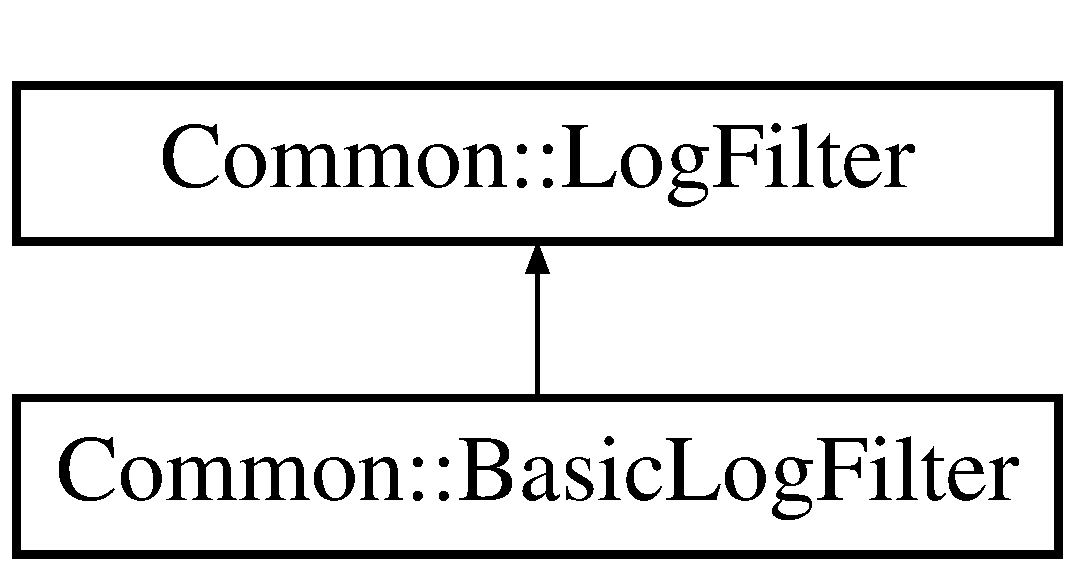
\includegraphics[height=2.000000cm]{class_common_1_1_log_filter}
\end{center}
\end{figure}
\subsection*{Public Member Functions}
\begin{DoxyCompactItemize}
\item 
\hypertarget{class_common_1_1_log_filter_aa866b9b88b43ca6eea8d9f66db7d18d7}{virtual \hyperlink{class_common_1_1_log_filter_aa866b9b88b43ca6eea8d9f66db7d18d7}{$\sim$\-Log\-Filter} ()}\label{class_common_1_1_log_filter_aa866b9b88b43ca6eea8d9f66db7d18d7}

\begin{DoxyCompactList}\small\item\em Constructor. \end{DoxyCompactList}\item 
virtual bool \hyperlink{class_common_1_1_log_filter_aebeae402434ad214e21321de025ee890}{Accept} (\hyperlink{class_common_1_1_log_entry}{Log\-Entry} const \&entry) const =0
\begin{DoxyCompactList}\small\item\em Filters log entry. \end{DoxyCompactList}\end{DoxyCompactItemize}


\subsection{Detailed Description}
Abstract class, validates logs. 

\begin{DoxyVersion}{Version}
1.\-0b 
\end{DoxyVersion}
\begin{DoxySince}{Since}
1.\-0b 
\end{DoxySince}
\begin{DoxyAuthor}{Author}
Ania Sikora, 2002 
\end{DoxyAuthor}


\subsection{Member Function Documentation}
\hypertarget{class_common_1_1_log_filter_aebeae402434ad214e21321de025ee890}{\index{Common\-::\-Log\-Filter@{Common\-::\-Log\-Filter}!Accept@{Accept}}
\index{Accept@{Accept}!Common::LogFilter@{Common\-::\-Log\-Filter}}
\subsubsection[{Accept}]{\setlength{\rightskip}{0pt plus 5cm}virtual bool Common\-::\-Log\-Filter\-::\-Accept (
\begin{DoxyParamCaption}
\item[{{\bf Log\-Entry} const \&}]{entry}
\end{DoxyParamCaption}
) const\hspace{0.3cm}{\ttfamily [pure virtual]}}}\label{class_common_1_1_log_filter_aebeae402434ad214e21321de025ee890}


Filters log entry. 

\begin{DoxyReturn}{Returns}
True if entry is accepted, false otherwise. 
\end{DoxyReturn}


Implemented in \hyperlink{class_common_1_1_basic_log_filter_a6dcb632906cd269b32a659633060b008}{Common\-::\-Basic\-Log\-Filter}.



The documentation for this class was generated from the following file\-:\begin{DoxyCompactItemize}
\item 
Common/Syslog.\-h\end{DoxyCompactItemize}

\hypertarget{class_common_1_1_log_formatter}{\section{Common\-:\-:Log\-Formatter Class Reference}
\label{class_common_1_1_log_formatter}\index{Common\-::\-Log\-Formatter@{Common\-::\-Log\-Formatter}}
}


Abstract class, Gives logs the correct format.  




{\ttfamily \#include $<$Syslog.\-h$>$}

Inheritance diagram for Common\-:\-:Log\-Formatter\-:\begin{figure}[H]
\begin{center}
\leavevmode
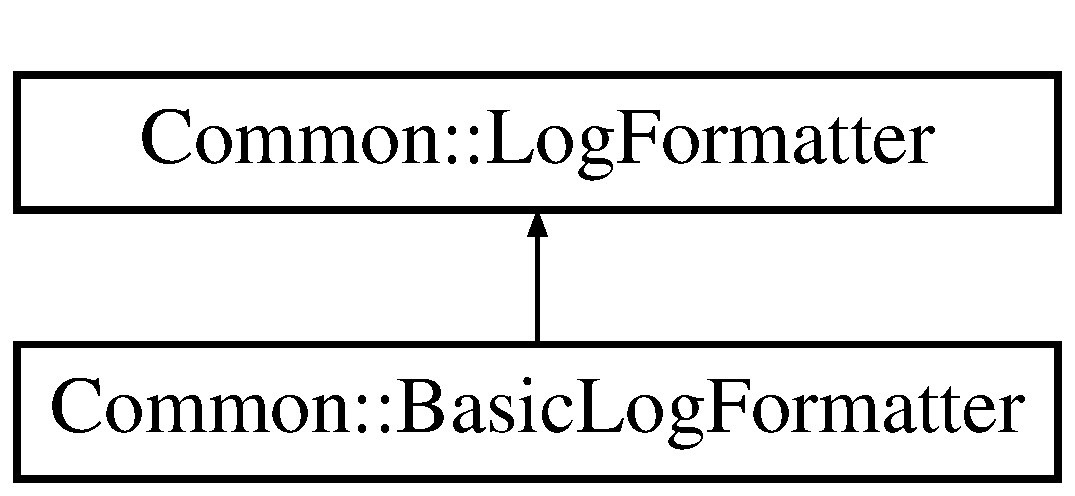
\includegraphics[height=2.000000cm]{class_common_1_1_log_formatter}
\end{center}
\end{figure}
\subsection*{Public Member Functions}
\begin{DoxyCompactItemize}
\item 
\hypertarget{class_common_1_1_log_formatter_a881b7156070a525a8c48fd24e2843ccd}{virtual \hyperlink{class_common_1_1_log_formatter_a881b7156070a525a8c48fd24e2843ccd}{$\sim$\-Log\-Formatter} ()}\label{class_common_1_1_log_formatter_a881b7156070a525a8c48fd24e2843ccd}

\begin{DoxyCompactList}\small\item\em Destructor. \end{DoxyCompactList}\item 
\hypertarget{class_common_1_1_log_formatter_a41ac9630f001955dd3496a4f74f8a50b}{virtual std\-::string \hyperlink{class_common_1_1_log_formatter_a41ac9630f001955dd3496a4f74f8a50b}{Get\-Log\-Header} () const =0}\label{class_common_1_1_log_formatter_a41ac9630f001955dd3496a4f74f8a50b}

\begin{DoxyCompactList}\small\item\em Returns a string containing the log header. \end{DoxyCompactList}\item 
\hypertarget{class_common_1_1_log_formatter_abb4ac3da1d04937ec42925a2da41a749}{virtual std\-::string \hyperlink{class_common_1_1_log_formatter_abb4ac3da1d04937ec42925a2da41a749}{Get\-Log\-Footer} () const =0}\label{class_common_1_1_log_formatter_abb4ac3da1d04937ec42925a2da41a749}

\begin{DoxyCompactList}\small\item\em Returns a string containing the log footer. \end{DoxyCompactList}\item 
\hypertarget{class_common_1_1_log_formatter_a4e4298a6c1f65b3cf40c757ca705b57d}{virtual std\-::string \hyperlink{class_common_1_1_log_formatter_a4e4298a6c1f65b3cf40c757ca705b57d}{Format} (\hyperlink{class_common_1_1_log_entry}{Log\-Entry} const \&entry) const =0}\label{class_common_1_1_log_formatter_a4e4298a6c1f65b3cf40c757ca705b57d}

\begin{DoxyCompactList}\small\item\em Returns a string containing the \hyperlink{class_common_1_1_log_entry}{Log\-Entry} object formatted. \end{DoxyCompactList}\end{DoxyCompactItemize}


\subsection{Detailed Description}
Abstract class, Gives logs the correct format. 

\begin{DoxyVersion}{Version}
1.\-0b 
\end{DoxyVersion}
\begin{DoxySince}{Since}
1.\-0b 
\end{DoxySince}
\begin{DoxyAuthor}{Author}
Ania Sikora, 2002 
\end{DoxyAuthor}


The documentation for this class was generated from the following file\-:\begin{DoxyCompactItemize}
\item 
Common/Syslog.\-h\end{DoxyCompactItemize}

\hypertarget{class_common_1_1_logger}{\section{Common\-:\-:Logger Class Reference}
\label{class_common_1_1_logger}\index{Common\-::\-Logger@{Common\-::\-Logger}}
}


Abstract class, tracks and stores information about events of interest happening in a system.  




{\ttfamily \#include $<$Syslog.\-h$>$}

Inheritance diagram for Common\-:\-:Logger\-:\begin{figure}[H]
\begin{center}
\leavevmode
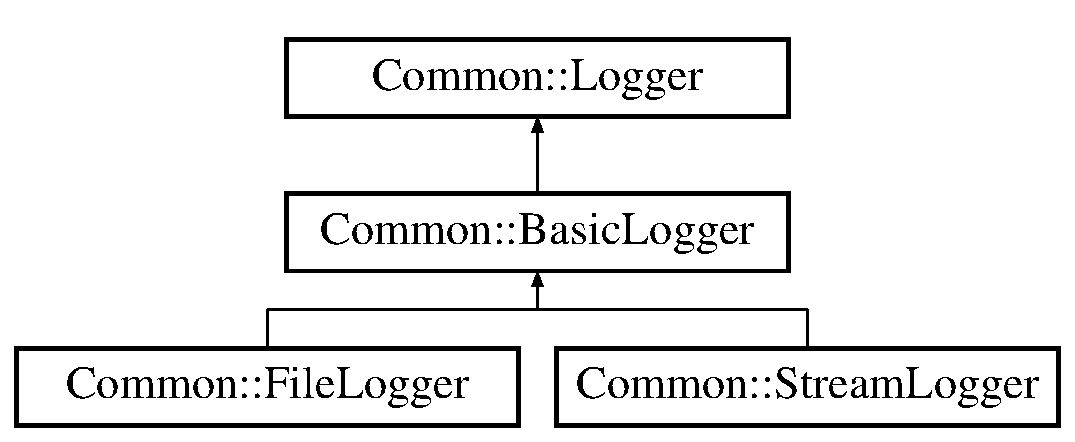
\includegraphics[height=3.000000cm]{class_common_1_1_logger}
\end{center}
\end{figure}
\subsection*{Public Member Functions}
\begin{DoxyCompactItemize}
\item 
\hypertarget{class_common_1_1_logger_af51d41dfc8d3ded5958beb128177dfc2}{virtual \hyperlink{class_common_1_1_logger_af51d41dfc8d3ded5958beb128177dfc2}{$\sim$\-Logger} ()}\label{class_common_1_1_logger_af51d41dfc8d3ded5958beb128177dfc2}

\begin{DoxyCompactList}\small\item\em Destructor. \end{DoxyCompactList}\item 
virtual void \hyperlink{class_common_1_1_logger_abf06fde5f12a512d49f4cd3cac61f28f}{Log} (\hyperlink{class_common_1_1_log_entry}{Log\-Entry} const \&entry)=0
\begin{DoxyCompactList}\small\item\em Constructor. \end{DoxyCompactList}\item 
\hypertarget{class_common_1_1_logger_aff7c2102e77ad6bc3e78a2f55ba8aff5}{void \hyperlink{class_common_1_1_logger_aff7c2102e77ad6bc3e78a2f55ba8aff5}{Set\-Name} (std\-::string const \&name)}\label{class_common_1_1_logger_aff7c2102e77ad6bc3e78a2f55ba8aff5}

\begin{DoxyCompactList}\small\item\em Sets logger name. \end{DoxyCompactList}\item 
\hypertarget{class_common_1_1_logger_a044d1cae9dbf0ffc0e476346b3199f3f}{std\-::string const \& \hyperlink{class_common_1_1_logger_a044d1cae9dbf0ffc0e476346b3199f3f}{Get\-Name} () const }\label{class_common_1_1_logger_a044d1cae9dbf0ffc0e476346b3199f3f}

\begin{DoxyCompactList}\small\item\em Returns a string containing the logger name. \end{DoxyCompactList}\item 
\hypertarget{class_common_1_1_logger_a9655d916e7e14956c61a5fb55f57d1e3}{virtual void \hyperlink{class_common_1_1_logger_a9655d916e7e14956c61a5fb55f57d1e3}{Set\-Filter} (Log\-Filter\-Ptr \&filter)=0}\label{class_common_1_1_logger_a9655d916e7e14956c61a5fb55f57d1e3}

\begin{DoxyCompactList}\small\item\em Sets the \hyperlink{class_common_1_1_log_filter}{Log\-Filter} to be used by the logger. \end{DoxyCompactList}\item 
\hypertarget{class_common_1_1_logger_a79e05daf2a2bf89829e3fb0876b2d335}{virtual \hyperlink{class_common_1_1_log_filter}{Log\-Filter} const $\ast$ \hyperlink{class_common_1_1_logger_a79e05daf2a2bf89829e3fb0876b2d335}{Get\-Filter} () const =0}\label{class_common_1_1_logger_a79e05daf2a2bf89829e3fb0876b2d335}

\begin{DoxyCompactList}\small\item\em Returns the \hyperlink{class_common_1_1_log_filter}{Log\-Filter} the logger uses. \end{DoxyCompactList}\item 
\hypertarget{class_common_1_1_logger_a9ac47b3569eac45a0cbb877339c702c2}{virtual void \hyperlink{class_common_1_1_logger_a9ac47b3569eac45a0cbb877339c702c2}{Set\-Formatter} (Log\-Formatter\-Ptr \&formatter)=0}\label{class_common_1_1_logger_a9ac47b3569eac45a0cbb877339c702c2}

\begin{DoxyCompactList}\small\item\em Sets the \hyperlink{class_common_1_1_log_formatter}{Log\-Formatter} to be used by the logger. \end{DoxyCompactList}\item 
\hypertarget{class_common_1_1_logger_a5e97af073499220bd7137531670fe3a4}{virtual \hyperlink{class_common_1_1_log_formatter}{Log\-Formatter} const $\ast$ \hyperlink{class_common_1_1_logger_a5e97af073499220bd7137531670fe3a4}{Get\-Formatter} () const =0}\label{class_common_1_1_logger_a5e97af073499220bd7137531670fe3a4}

\begin{DoxyCompactList}\small\item\em Returns the \hyperlink{class_common_1_1_log_formatter}{Log\-Formatter} the logger uses. \end{DoxyCompactList}\end{DoxyCompactItemize}


\subsection{Detailed Description}
Abstract class, tracks and stores information about events of interest happening in a system. 

\begin{DoxyVersion}{Version}
1.\-0b 
\end{DoxyVersion}
\begin{DoxySince}{Since}
1.\-0b 
\end{DoxySince}
\begin{DoxyAuthor}{Author}
Ania Sikora, 2002 
\end{DoxyAuthor}


\subsection{Member Function Documentation}
\hypertarget{class_common_1_1_logger_abf06fde5f12a512d49f4cd3cac61f28f}{\index{Common\-::\-Logger@{Common\-::\-Logger}!Log@{Log}}
\index{Log@{Log}!Common::Logger@{Common\-::\-Logger}}
\subsubsection[{Log}]{\setlength{\rightskip}{0pt plus 5cm}virtual void Common\-::\-Logger\-::\-Log (
\begin{DoxyParamCaption}
\item[{{\bf Log\-Entry} const \&}]{entry}
\end{DoxyParamCaption}
)\hspace{0.3cm}{\ttfamily [pure virtual]}}}\label{class_common_1_1_logger_abf06fde5f12a512d49f4cd3cac61f28f}


Constructor. 


\begin{DoxyParams}{Parameters}
{\em entry} & \\
\hline
\end{DoxyParams}


Implemented in \hyperlink{class_common_1_1_file_logger_a2f487ff3e7c10476f371e5cc7166a6f3}{Common\-::\-File\-Logger}, and \hyperlink{class_common_1_1_stream_logger_ad6176e77665c3d383469d492121d7ece}{Common\-::\-Stream\-Logger}.



The documentation for this class was generated from the following file\-:\begin{DoxyCompactItemize}
\item 
Common/Syslog.\-h\end{DoxyCompactItemize}

\hypertarget{struct_model_param}{\section{Model\-Param Struct Reference}
\label{struct_model_param}\index{Model\-Param@{Model\-Param}}
}


Stores the total volume of data, the total amount of data sent by workers and the total computed time.  




{\ttfamily \#include $<$Factoring\-Stats\-\_\-nw.\-h$>$}

\subsection*{Public Attributes}
\begin{DoxyCompactItemize}
\item 
\hypertarget{struct_model_param_aaad2643381b3ba13d8d4ed96870d9dcd}{int {\bfseries Total\-Data\-Volume}}\label{struct_model_param_aaad2643381b3ba13d8d4ed96870d9dcd}

\item 
\hypertarget{struct_model_param_a51557b4c87cc22ed4af4fcbeaa9416ac}{int {\bfseries Total\-Data\-Send\-W}}\label{struct_model_param_a51557b4c87cc22ed4af4fcbeaa9416ac}

\item 
\hypertarget{struct_model_param_a879ce9946920b2c1846d9b0916ce6dad}{double {\bfseries Total\-Comp\-Time}}\label{struct_model_param_a879ce9946920b2c1846d9b0916ce6dad}

\end{DoxyCompactItemize}


\subsection{Detailed Description}
Stores the total volume of data, the total amount of data sent by workers and the total computed time. 

The documentation for this struct was generated from the following file\-:\begin{DoxyCompactItemize}
\item 
Analyzer/Factoring\-Stats\-\_\-nw.\-h\end{DoxyCompactItemize}

\hypertarget{class_module_list}{\section{Module\-List Class Reference}
\label{class_module_list}\index{Module\-List@{Module\-List}}
}


Class that stores and handles a vector of B\-Patch\-\_\-modules.  




{\ttfamily \#include $<$di.\-h$>$}

\subsection*{Public Member Functions}
\begin{DoxyCompactItemize}
\item 
\hyperlink{class_module_list_a184b4e31f6e1df914701a43055215a88}{Module\-List} (B\-Patch\-\_\-image \&bp\-Image)
\begin{DoxyCompactList}\small\item\em Constructor. \end{DoxyCompactList}\item 
int \hyperlink{class_module_list_a30e1ca8e40ebc1ce371fa6925031c6c8}{Get\-Size} () const 
\begin{DoxyCompactList}\small\item\em Getter of the vector size. \end{DoxyCompactList}\item 
\hypertarget{class_module_list_a5c0f811ee4768944e73bc024e0e97588}{B\-Patch\-\_\-module \& {\bfseries operator\mbox{[}$\,$\mbox{]}} (int i) const }\label{class_module_list_a5c0f811ee4768944e73bc024e0e97588}

\end{DoxyCompactItemize}


\subsection{Detailed Description}
Class that stores and handles a vector of B\-Patch\-\_\-modules. 

\begin{DoxyVersion}{Version}
1.\-0b 
\end{DoxyVersion}
\begin{DoxyAuthor}{Author}
Ania Sikora, 2002 
\end{DoxyAuthor}
\begin{DoxySince}{Since}
1.\-0b 
\end{DoxySince}


\subsection{Constructor \& Destructor Documentation}
\hypertarget{class_module_list_a184b4e31f6e1df914701a43055215a88}{\index{Module\-List@{Module\-List}!Module\-List@{Module\-List}}
\index{Module\-List@{Module\-List}!ModuleList@{Module\-List}}
\subsubsection[{Module\-List}]{\setlength{\rightskip}{0pt plus 5cm}Module\-List\-::\-Module\-List (
\begin{DoxyParamCaption}
\item[{B\-Patch\-\_\-image \&}]{bp\-Image}
\end{DoxyParamCaption}
)\hspace{0.3cm}{\ttfamily [inline]}}}\label{class_module_list_a184b4e31f6e1df914701a43055215a88}


Constructor. 


\begin{DoxyParams}{Parameters}
{\em bp\-Image} & Program image \\
\hline
\end{DoxyParams}


\subsection{Member Function Documentation}
\hypertarget{class_module_list_a30e1ca8e40ebc1ce371fa6925031c6c8}{\index{Module\-List@{Module\-List}!Get\-Size@{Get\-Size}}
\index{Get\-Size@{Get\-Size}!ModuleList@{Module\-List}}
\subsubsection[{Get\-Size}]{\setlength{\rightskip}{0pt plus 5cm}int Module\-List\-::\-Get\-Size (
\begin{DoxyParamCaption}
{}
\end{DoxyParamCaption}
) const\hspace{0.3cm}{\ttfamily [inline]}}}\label{class_module_list_a30e1ca8e40ebc1ce371fa6925031c6c8}


Getter of the vector size. 

\begin{DoxyReturn}{Returns}
\-\_\-vector-\/$>$size 
\end{DoxyReturn}


The documentation for this class was generated from the following file\-:\begin{DoxyCompactItemize}
\item 
Common/di.\-h\end{DoxyCompactItemize}

\hypertarget{class_monitor}{\section{Monitor Class Reference}
\label{class_monitor}\index{Monitor@{Monitor}}
}


Adds request to add or remove instrumentation in/from the tasks that it is monitoring.  




{\ttfamily \#include $<$Monitor.\-h$>$}

\subsection*{Public Member Functions}
\begin{DoxyCompactItemize}
\item 
\hyperlink{class_monitor_a40a03e4b9ea61cb3394956cebebfddeb}{Monitor} (\hyperlink{class_task_collection}{Task\-Collection} \&tasks)
\begin{DoxyCompactList}\small\item\em Constructor. \end{DoxyCompactList}\item 
void \hyperlink{class_monitor_a45d639b99e3a7152b90f722fc64ad2f8}{Add\-Instr} (\hyperlink{class_common_1_1_add_instr_request}{Add\-Instr\-Request} \&instr\-Req)
\begin{DoxyCompactList}\small\item\em Adds the instructions requested to the task they belong to. \end{DoxyCompactList}\item 
void \hyperlink{class_monitor_addc6c841719134e41cc6c773f7e3eff9}{Remove\-Instr} (\hyperlink{class_common_1_1_remove_instr_request}{Remove\-Instr\-Request} \&instr\-Req)
\begin{DoxyCompactList}\small\item\em Removes the instructions requested from the selected task. \end{DoxyCompactList}\end{DoxyCompactItemize}


\subsection{Detailed Description}
Adds request to add or remove instrumentation in/from the tasks that it is monitoring. 

\begin{DoxyVersion}{Version}
1.\-0 
\end{DoxyVersion}
\begin{DoxySince}{Since}
1.\-0 
\end{DoxySince}
\begin{DoxyAuthor}{Author}
Ania Sikora, 2002 
\end{DoxyAuthor}


\subsection{Constructor \& Destructor Documentation}
\hypertarget{class_monitor_a40a03e4b9ea61cb3394956cebebfddeb}{\index{Monitor@{Monitor}!Monitor@{Monitor}}
\index{Monitor@{Monitor}!Monitor@{Monitor}}
\subsubsection[{Monitor}]{\setlength{\rightskip}{0pt plus 5cm}Monitor\-::\-Monitor (
\begin{DoxyParamCaption}
\item[{{\bf Task\-Collection} \&}]{tasks}
\end{DoxyParamCaption}
)\hspace{0.3cm}{\ttfamily [inline]}}}\label{class_monitor_a40a03e4b9ea61cb3394956cebebfddeb}


Constructor. 


\begin{DoxyParams}{Parameters}
{\em tasks} & Collection of tasks susceptible to be modified. \\
\hline
\end{DoxyParams}


\subsection{Member Function Documentation}
\hypertarget{class_monitor_a45d639b99e3a7152b90f722fc64ad2f8}{\index{Monitor@{Monitor}!Add\-Instr@{Add\-Instr}}
\index{Add\-Instr@{Add\-Instr}!Monitor@{Monitor}}
\subsubsection[{Add\-Instr}]{\setlength{\rightskip}{0pt plus 5cm}void Monitor\-::\-Add\-Instr (
\begin{DoxyParamCaption}
\item[{{\bf Add\-Instr\-Request} \&}]{instr\-Req}
\end{DoxyParamCaption}
)}}\label{class_monitor_a45d639b99e3a7152b90f722fc64ad2f8}


Adds the instructions requested to the task they belong to. 


\begin{DoxyParams}{Parameters}
{\em inst\-Req} & Object that represents the request for instrumentation to be added to a task. \\
\hline
\end{DoxyParams}
\hypertarget{class_monitor_addc6c841719134e41cc6c773f7e3eff9}{\index{Monitor@{Monitor}!Remove\-Instr@{Remove\-Instr}}
\index{Remove\-Instr@{Remove\-Instr}!Monitor@{Monitor}}
\subsubsection[{Remove\-Instr}]{\setlength{\rightskip}{0pt plus 5cm}void Monitor\-::\-Remove\-Instr (
\begin{DoxyParamCaption}
\item[{{\bf Remove\-Instr\-Request} \&}]{instr\-Req}
\end{DoxyParamCaption}
)}}\label{class_monitor_addc6c841719134e41cc6c773f7e3eff9}


Removes the instructions requested from the selected task. 


\begin{DoxyParams}{Parameters}
{\em inst\-Req} & Object that represents the request for instrumentation to be removed from a task. \\
\hline
\end{DoxyParams}


The documentation for this class was generated from the following files\-:\begin{DoxyCompactItemize}
\item 
A\-C/Monitor.\-h\item 
A\-C/Monitor.\-cpp\end{DoxyCompactItemize}

\hypertarget{class_common_1_1_mutex}{\section{Common\-:\-:Mutex Class Reference}
\label{class_common_1_1_mutex}\index{Common\-::\-Mutex@{Common\-::\-Mutex}}
}


Guarantees non concurrent access to a resource.  




{\ttfamily \#include $<$sync.\-h$>$}

\subsection*{Public Member Functions}
\begin{DoxyCompactItemize}
\item 
\hyperlink{class_common_1_1_mutex_aad803448fe15d30cb4a2547530dec2d8}{Mutex} ()
\begin{DoxyCompactList}\small\item\em Constructor. \end{DoxyCompactList}\item 
\hypertarget{class_common_1_1_mutex_afbf95aaaee6cd901b93e10b94d9599d4}{\hyperlink{class_common_1_1_mutex_afbf95aaaee6cd901b93e10b94d9599d4}{$\sim$\-Mutex} ()}\label{class_common_1_1_mutex_afbf95aaaee6cd901b93e10b94d9599d4}

\begin{DoxyCompactList}\small\item\em Destructor. \end{DoxyCompactList}\item 
\hypertarget{class_common_1_1_mutex_a117ceec3b486ec875b375114eca81cce}{{\bfseries operator pthread\-\_\-mutex\-\_\-t $\ast$} ()}\label{class_common_1_1_mutex_a117ceec3b486ec875b375114eca81cce}

\end{DoxyCompactItemize}
\subsection*{Protected Member Functions}
\begin{DoxyCompactItemize}
\item 
void \hyperlink{class_common_1_1_mutex_a08adde4760931f79a7ae7702cde3c034}{Enter} ()
\begin{DoxyCompactList}\small\item\em Denotes that someone starts using the resource. \end{DoxyCompactList}\item 
\hypertarget{class_common_1_1_mutex_a5b4ef7e61426f2e7c17e12449e55b353}{bool \hyperlink{class_common_1_1_mutex_a5b4ef7e61426f2e7c17e12449e55b353}{Can\-Enter} ()}\label{class_common_1_1_mutex_a5b4ef7e61426f2e7c17e12449e55b353}

\begin{DoxyCompactList}\small\item\em Returns true if the resource is not being used, false otherwise. \end{DoxyCompactList}\item 
void \hyperlink{class_common_1_1_mutex_a59b41bf53521202af2c59201cd078aab}{Leave} ()
\begin{DoxyCompactList}\small\item\em Denotes that someone stops using the resource. \end{DoxyCompactList}\end{DoxyCompactItemize}
\subsection*{Friends}
\begin{DoxyCompactItemize}
\item 
\hypertarget{class_common_1_1_mutex_a7177018259362468923e579d8525b5d5}{class {\bfseries Mutex\-Lock}}\label{class_common_1_1_mutex_a7177018259362468923e579d8525b5d5}

\end{DoxyCompactItemize}


\subsection{Detailed Description}
Guarantees non concurrent access to a resource. 

Mutual-\/\-Exclusion Object

\begin{DoxyVersion}{Version}
1.\-0b 
\end{DoxyVersion}
\begin{DoxySince}{Since}
1.\-0b 
\end{DoxySince}
\begin{DoxyAuthor}{Author}
Ania Sikora, 2002 
\end{DoxyAuthor}


\subsection{Constructor \& Destructor Documentation}
\hypertarget{class_common_1_1_mutex_aad803448fe15d30cb4a2547530dec2d8}{\index{Common\-::\-Mutex@{Common\-::\-Mutex}!Mutex@{Mutex}}
\index{Mutex@{Mutex}!Common::Mutex@{Common\-::\-Mutex}}
\subsubsection[{Mutex}]{\setlength{\rightskip}{0pt plus 5cm}Common\-::\-Mutex\-::\-Mutex (
\begin{DoxyParamCaption}
{}
\end{DoxyParamCaption}
)\hspace{0.3cm}{\ttfamily [inline]}}}\label{class_common_1_1_mutex_aad803448fe15d30cb4a2547530dec2d8}


Constructor. 

The mutex is always initialized as a recursive entity. 

\subsection{Member Function Documentation}
\hypertarget{class_common_1_1_mutex_a08adde4760931f79a7ae7702cde3c034}{\index{Common\-::\-Mutex@{Common\-::\-Mutex}!Enter@{Enter}}
\index{Enter@{Enter}!Common::Mutex@{Common\-::\-Mutex}}
\subsubsection[{Enter}]{\setlength{\rightskip}{0pt plus 5cm}void Mutex\-::\-Enter (
\begin{DoxyParamCaption}
{}
\end{DoxyParamCaption}
)\hspace{0.3cm}{\ttfamily [protected]}}}\label{class_common_1_1_mutex_a08adde4760931f79a7ae7702cde3c034}


Denotes that someone starts using the resource. 


\begin{DoxyExceptions}{Exceptions}
{\em \hyperlink{class_common_1_1_sys_exception}{Sys\-Exception}} & \\
\hline
\end{DoxyExceptions}
\hypertarget{class_common_1_1_mutex_a59b41bf53521202af2c59201cd078aab}{\index{Common\-::\-Mutex@{Common\-::\-Mutex}!Leave@{Leave}}
\index{Leave@{Leave}!Common::Mutex@{Common\-::\-Mutex}}
\subsubsection[{Leave}]{\setlength{\rightskip}{0pt plus 5cm}void Mutex\-::\-Leave (
\begin{DoxyParamCaption}
{}
\end{DoxyParamCaption}
)\hspace{0.3cm}{\ttfamily [protected]}}}\label{class_common_1_1_mutex_a59b41bf53521202af2c59201cd078aab}


Denotes that someone stops using the resource. 


\begin{DoxyExceptions}{Exceptions}
{\em \hyperlink{class_common_1_1_sys_exception}{Sys\-Exception}} & \\
\hline
\end{DoxyExceptions}


The documentation for this class was generated from the following files\-:\begin{DoxyCompactItemize}
\item 
Common/sync.\-h\item 
Common/sync.\-cpp\end{DoxyCompactItemize}

\hypertarget{class_common_1_1_mutex_lock}{\section{Common\-:\-:Mutex\-Lock Class Reference}
\label{class_common_1_1_mutex_lock}\index{Common\-::\-Mutex\-Lock@{Common\-::\-Mutex\-Lock}}
}


System to manage access to a resource with a mutex.  




{\ttfamily \#include $<$sync.\-h$>$}

\subsection*{Public Member Functions}
\begin{DoxyCompactItemize}
\item 
\hypertarget{class_common_1_1_mutex_lock_a9004e1a2a9c4202a74962c36ad21e018}{\hyperlink{class_common_1_1_mutex_lock_a9004e1a2a9c4202a74962c36ad21e018}{Mutex\-Lock} (\hyperlink{class_common_1_1_mutex}{Mutex} \&mutex)}\label{class_common_1_1_mutex_lock_a9004e1a2a9c4202a74962c36ad21e018}

\begin{DoxyCompactList}\small\item\em Constructor. \end{DoxyCompactList}\item 
\hypertarget{class_common_1_1_mutex_lock_affd89ce38a023916e8dee3e018b57b1c}{\hyperlink{class_common_1_1_mutex_lock_affd89ce38a023916e8dee3e018b57b1c}{$\sim$\-Mutex\-Lock} ()}\label{class_common_1_1_mutex_lock_affd89ce38a023916e8dee3e018b57b1c}

\begin{DoxyCompactList}\small\item\em Destructor. \end{DoxyCompactList}\end{DoxyCompactItemize}


\subsection{Detailed Description}
System to manage access to a resource with a mutex. 

\begin{DoxyVersion}{Version}
1.\-0b 
\end{DoxyVersion}
\begin{DoxySince}{Since}
1.\-0b 
\end{DoxySince}
\begin{DoxyAuthor}{Author}
Ania Sikora, 2002 
\end{DoxyAuthor}


The documentation for this class was generated from the following file\-:\begin{DoxyCompactItemize}
\item 
Common/sync.\-h\end{DoxyCompactItemize}

\hypertarget{classmyauto__ptr}{\section{myauto\-\_\-ptr$<$ X $>$ Class Template Reference}
\label{classmyauto__ptr}\index{myauto\-\_\-ptr$<$ X $>$@{myauto\-\_\-ptr$<$ X $>$}}
}
\subsection*{Public Types}
\begin{DoxyCompactItemize}
\item 
\hypertarget{classmyauto__ptr_a5bd4197c8d3825450a05fee341b194c2}{typedef X {\bfseries element\-\_\-type}}\label{classmyauto__ptr_a5bd4197c8d3825450a05fee341b194c2}

\end{DoxyCompactItemize}
\subsection*{Public Member Functions}
\begin{DoxyCompactItemize}
\item 
\hypertarget{classmyauto__ptr_ac80c5eed05ad474f4719aec620cc2276}{{\bfseries myauto\-\_\-ptr} (X $\ast$p=0)}\label{classmyauto__ptr_ac80c5eed05ad474f4719aec620cc2276}

\item 
\hypertarget{classmyauto__ptr_a5516d4846374475d72f9636b992d3e20}{{\bfseries myauto\-\_\-ptr} (const \hyperlink{classmyauto__ptr}{myauto\-\_\-ptr} \&a)}\label{classmyauto__ptr_a5516d4846374475d72f9636b992d3e20}

\item 
\hypertarget{classmyauto__ptr_acd9f62ccfbcc73e6d35f7d26b2619b5f}{\hyperlink{classmyauto__ptr}{myauto\-\_\-ptr} \& {\bfseries operator=} (const \hyperlink{classmyauto__ptr}{myauto\-\_\-ptr} \&a)}\label{classmyauto__ptr_acd9f62ccfbcc73e6d35f7d26b2619b5f}

\item 
\hypertarget{classmyauto__ptr_a79c8ab801437d45a55eb9546095dc287}{X \& {\bfseries operator$\ast$} () const }\label{classmyauto__ptr_a79c8ab801437d45a55eb9546095dc287}

\item 
\hypertarget{classmyauto__ptr_a6765cc8f5e07d883b05cd05a2fa3e626}{X $\ast$ {\bfseries operator-\/$>$} () const }\label{classmyauto__ptr_a6765cc8f5e07d883b05cd05a2fa3e626}

\item 
\hypertarget{classmyauto__ptr_a8dc00ddeecc31e7c9c0c54420342877c}{X $\ast$ {\bfseries get} () const }\label{classmyauto__ptr_a8dc00ddeecc31e7c9c0c54420342877c}

\item 
\hypertarget{classmyauto__ptr_ab0d144c02d4cf2496e6821fdd60d56bd}{X $\ast$ {\bfseries release} () const }\label{classmyauto__ptr_ab0d144c02d4cf2496e6821fdd60d56bd}

\end{DoxyCompactItemize}


The documentation for this class was generated from the following file\-:\begin{DoxyCompactItemize}
\item 
Common/auto\-\_\-ptr.\-h\end{DoxyCompactItemize}

\hypertarget{class_common_1_1_network_de_serializer}{\section{Common\-:\-:Network\-De\-Serializer Class Reference}
\label{class_common_1_1_network_de_serializer}\index{Common\-::\-Network\-De\-Serializer@{Common\-::\-Network\-De\-Serializer}}
}


Extracts serialized data from an istream object.  




{\ttfamily \#include $<$Net\-Ser.\-h$>$}

Inheritance diagram for Common\-:\-:Network\-De\-Serializer\-:\begin{figure}[H]
\begin{center}
\leavevmode
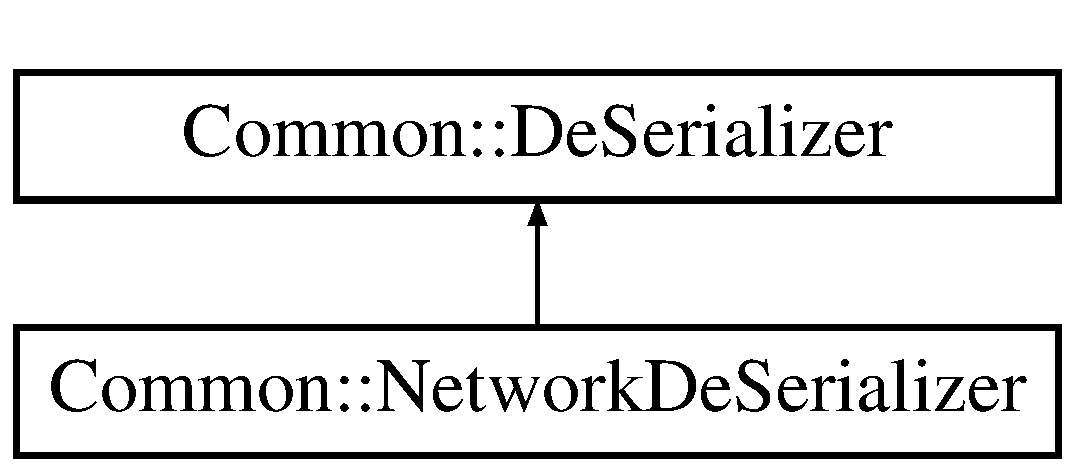
\includegraphics[height=2.000000cm]{class_common_1_1_network_de_serializer}
\end{center}
\end{figure}
\subsection*{Public Member Functions}
\begin{DoxyCompactItemize}
\item 
\hypertarget{class_common_1_1_network_de_serializer_a291e095c279f2b58bfc2433afb5a4b13}{\hyperlink{class_common_1_1_network_de_serializer_a291e095c279f2b58bfc2433afb5a4b13}{Network\-De\-Serializer} (std\-::istream \&stream)}\label{class_common_1_1_network_de_serializer_a291e095c279f2b58bfc2433afb5a4b13}

\begin{DoxyCompactList}\small\item\em Constructor. \end{DoxyCompactList}\item 
\hypertarget{class_common_1_1_network_de_serializer_ae5450dc7c8503b1190f0be4426e86d7a}{std\-::istream \& \hyperlink{class_common_1_1_network_de_serializer_ae5450dc7c8503b1190f0be4426e86d7a}{Get\-Stream} ()}\label{class_common_1_1_network_de_serializer_ae5450dc7c8503b1190f0be4426e86d7a}

\begin{DoxyCompactList}\small\item\em Returns istream object where the data is serialized. \end{DoxyCompactList}\item 
\hypertarget{class_common_1_1_network_de_serializer_a3107f346baa11ebadb4ee99713257b20}{long\-\_\-t \hyperlink{class_common_1_1_network_de_serializer_a3107f346baa11ebadb4ee99713257b20}{Get\-Long} ()}\label{class_common_1_1_network_de_serializer_a3107f346baa11ebadb4ee99713257b20}

\begin{DoxyCompactList}\small\item\em Reads long value from the stream. \end{DoxyCompactList}\item 
\hypertarget{class_common_1_1_network_de_serializer_aac6d6a2af87969464cc719d8a35bf2d7}{double\-\_\-t \hyperlink{class_common_1_1_network_de_serializer_aac6d6a2af87969464cc719d8a35bf2d7}{Get\-Double} ()}\label{class_common_1_1_network_de_serializer_aac6d6a2af87969464cc719d8a35bf2d7}

\begin{DoxyCompactList}\small\item\em Reads double value from the stream. \end{DoxyCompactList}\item 
\hypertarget{class_common_1_1_network_de_serializer_a8ec118436044b285a64a2b19f2b94e4e}{bool\-\_\-t \hyperlink{class_common_1_1_network_de_serializer_a8ec118436044b285a64a2b19f2b94e4e}{Get\-Bool} ()}\label{class_common_1_1_network_de_serializer_a8ec118436044b285a64a2b19f2b94e4e}

\begin{DoxyCompactList}\small\item\em Reads bool value from the stream. \end{DoxyCompactList}\item 
\hypertarget{class_common_1_1_network_de_serializer_a9c9aa5085668168f71562a84daade8a6}{short\-\_\-t \hyperlink{class_common_1_1_network_de_serializer_a9c9aa5085668168f71562a84daade8a6}{Get\-Short} ()}\label{class_common_1_1_network_de_serializer_a9c9aa5085668168f71562a84daade8a6}

\begin{DoxyCompactList}\small\item\em Reads short value from the stream. \end{DoxyCompactList}\item 
\hypertarget{class_common_1_1_network_de_serializer_a75d49dc63c2b2804603f9d4a80cc6919}{byte\-\_\-t \hyperlink{class_common_1_1_network_de_serializer_a75d49dc63c2b2804603f9d4a80cc6919}{Get\-Byte} ()}\label{class_common_1_1_network_de_serializer_a75d49dc63c2b2804603f9d4a80cc6919}

\begin{DoxyCompactList}\small\item\em Reads byte value from the stream. \end{DoxyCompactList}\item 
\hypertarget{class_common_1_1_network_de_serializer_a60b30b4bb766fd2ee7ea1aed7a622a2f}{char\-\_\-t \hyperlink{class_common_1_1_network_de_serializer_a60b30b4bb766fd2ee7ea1aed7a622a2f}{Get\-Char} ()}\label{class_common_1_1_network_de_serializer_a60b30b4bb766fd2ee7ea1aed7a622a2f}

\begin{DoxyCompactList}\small\item\em Reads char value from the stream. \end{DoxyCompactList}\item 
\hypertarget{class_common_1_1_network_de_serializer_accae514d71b4edb181819b42cdd84f96}{std\-::string \hyperlink{class_common_1_1_network_de_serializer_accae514d71b4edb181819b42cdd84f96}{Get\-String} ()}\label{class_common_1_1_network_de_serializer_accae514d71b4edb181819b42cdd84f96}

\begin{DoxyCompactList}\small\item\em Reads string value from the stream. \end{DoxyCompactList}\item 
\hypertarget{class_common_1_1_network_de_serializer_abf9b6cc5269157ca81bb4f06cd5b1a61}{int\-\_\-t \hyperlink{class_common_1_1_network_de_serializer_abf9b6cc5269157ca81bb4f06cd5b1a61}{Get\-Int} ()}\label{class_common_1_1_network_de_serializer_abf9b6cc5269157ca81bb4f06cd5b1a61}

\begin{DoxyCompactList}\small\item\em Reads int value from the stream. \end{DoxyCompactList}\item 
\hypertarget{class_common_1_1_network_de_serializer_a4c5d801b6d105f91e475f6e6387f702b}{void \hyperlink{class_common_1_1_network_de_serializer_a4c5d801b6d105f91e475f6e6387f702b}{Get\-Buffer} (char $\ast$buffer, int buffer\-Size)}\label{class_common_1_1_network_de_serializer_a4c5d801b6d105f91e475f6e6387f702b}

\begin{DoxyCompactList}\small\item\em Reads data directly from the stream. \end{DoxyCompactList}\end{DoxyCompactItemize}


\subsection{Detailed Description}
Extracts serialized data from an istream object. 

\begin{DoxyVersion}{Version}
1.\-0b 
\end{DoxyVersion}
\begin{DoxySince}{Since}
1.\-0b 
\end{DoxySince}
\begin{DoxyAuthor}{Author}
Ania Sikora, 2002 
\end{DoxyAuthor}


The documentation for this class was generated from the following files\-:\begin{DoxyCompactItemize}
\item 
Common/Net\-Ser.\-h\item 
Common/Net\-Ser.\-cpp\end{DoxyCompactItemize}

\hypertarget{class_common_1_1_network_serializer}{\section{Common\-:\-:Network\-Serializer Class Reference}
\label{class_common_1_1_network_serializer}\index{Common\-::\-Network\-Serializer@{Common\-::\-Network\-Serializer}}
}


Puts serialized data into an \hyperlink{class_common_1_1_output_stream}{Output\-Stream} object.  




{\ttfamily \#include $<$Net\-Ser.\-h$>$}

Inheritance diagram for Common\-:\-:Network\-Serializer\-:\begin{figure}[H]
\begin{center}
\leavevmode
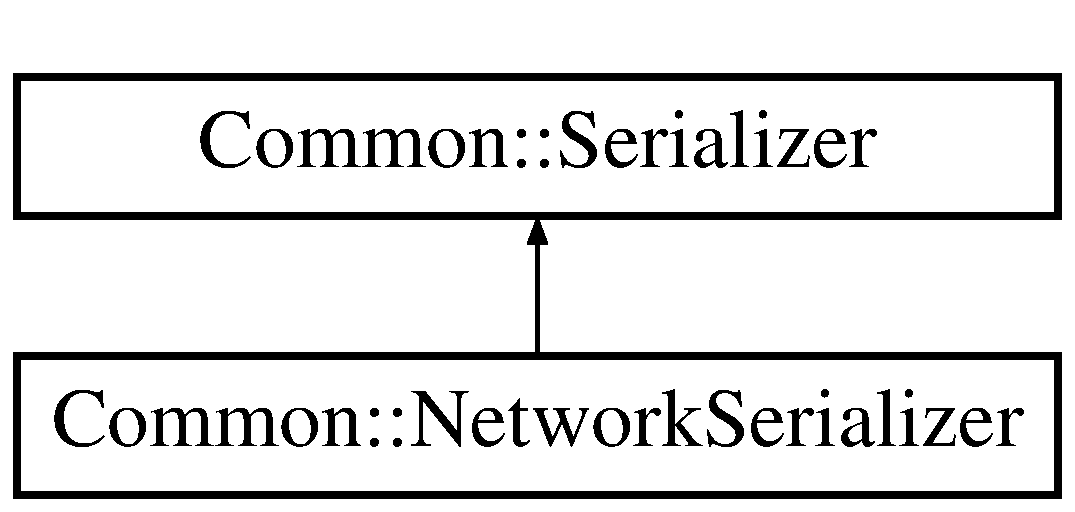
\includegraphics[height=2.000000cm]{class_common_1_1_network_serializer}
\end{center}
\end{figure}
\subsection*{Public Member Functions}
\begin{DoxyCompactItemize}
\item 
\hyperlink{class_common_1_1_network_serializer_a886a55466be3531c3b8cfa13cf029c7e}{Network\-Serializer} (\hyperlink{class_common_1_1_output_stream}{Output\-Stream} \&stream)
\begin{DoxyCompactList}\small\item\em Constructor. \end{DoxyCompactList}\item 
\hypertarget{class_common_1_1_network_serializer_a13e38d2db5b3583ed6265f68568e48cd}{void \hyperlink{class_common_1_1_network_serializer_a13e38d2db5b3583ed6265f68568e48cd}{Put\-Long} (long\-\_\-t l)}\label{class_common_1_1_network_serializer_a13e38d2db5b3583ed6265f68568e48cd}

\begin{DoxyCompactList}\small\item\em Puts a long into the stream. \end{DoxyCompactList}\item 
\hypertarget{class_common_1_1_network_serializer_acac3ed81f0c658d919365fd384508301}{void \hyperlink{class_common_1_1_network_serializer_acac3ed81f0c658d919365fd384508301}{Put\-Double} (double\-\_\-t d)}\label{class_common_1_1_network_serializer_acac3ed81f0c658d919365fd384508301}

\begin{DoxyCompactList}\small\item\em Puts a double into the stream. \end{DoxyCompactList}\item 
\hypertarget{class_common_1_1_network_serializer_a85591a5747364e3f372474ba8273322e}{void \hyperlink{class_common_1_1_network_serializer_a85591a5747364e3f372474ba8273322e}{Put\-Bool} (bool\-\_\-t b)}\label{class_common_1_1_network_serializer_a85591a5747364e3f372474ba8273322e}

\begin{DoxyCompactList}\small\item\em Puts a boolean into the stream. \end{DoxyCompactList}\item 
\hypertarget{class_common_1_1_network_serializer_a9000854e6736ee5d066bc89f493f0133}{void \hyperlink{class_common_1_1_network_serializer_a9000854e6736ee5d066bc89f493f0133}{Put\-Short} (short\-\_\-t s)}\label{class_common_1_1_network_serializer_a9000854e6736ee5d066bc89f493f0133}

\begin{DoxyCompactList}\small\item\em Puts a short into the stream. \end{DoxyCompactList}\item 
\hypertarget{class_common_1_1_network_serializer_ab5b1159c873c9edd318497c719eedc99}{void \hyperlink{class_common_1_1_network_serializer_ab5b1159c873c9edd318497c719eedc99}{Put\-Byte} (byte\-\_\-t b)}\label{class_common_1_1_network_serializer_ab5b1159c873c9edd318497c719eedc99}

\begin{DoxyCompactList}\small\item\em Puts a byte into the stream. \end{DoxyCompactList}\item 
\hypertarget{class_common_1_1_network_serializer_a35daf5250ffad493a6044d8089af1fc1}{void \hyperlink{class_common_1_1_network_serializer_a35daf5250ffad493a6044d8089af1fc1}{Put\-Char} (char\-\_\-t c)}\label{class_common_1_1_network_serializer_a35daf5250ffad493a6044d8089af1fc1}

\begin{DoxyCompactList}\small\item\em Puts a char into the stream. \end{DoxyCompactList}\item 
\hypertarget{class_common_1_1_network_serializer_a3fe79557a89ef5a84107802d3bf40a37}{void \hyperlink{class_common_1_1_network_serializer_a3fe79557a89ef5a84107802d3bf40a37}{Put\-String} (std\-::string const \&str)}\label{class_common_1_1_network_serializer_a3fe79557a89ef5a84107802d3bf40a37}

\begin{DoxyCompactList}\small\item\em Puts a string into the stream. \end{DoxyCompactList}\item 
\hypertarget{class_common_1_1_network_serializer_afe96d68e5efdd2d51a4acab621feba63}{void \hyperlink{class_common_1_1_network_serializer_afe96d68e5efdd2d51a4acab621feba63}{Put\-Int} (int\-\_\-t i)}\label{class_common_1_1_network_serializer_afe96d68e5efdd2d51a4acab621feba63}

\begin{DoxyCompactList}\small\item\em Puts an integer long into the stream. \end{DoxyCompactList}\item 
\hypertarget{class_common_1_1_network_serializer_a9cc1403e8ae617484e82e97364ce5e7d}{void \hyperlink{class_common_1_1_network_serializer_a9cc1403e8ae617484e82e97364ce5e7d}{Put\-Buffer} (char const $\ast$buffer, int buffer\-Size)}\label{class_common_1_1_network_serializer_a9cc1403e8ae617484e82e97364ce5e7d}

\begin{DoxyCompactList}\small\item\em Puts a buffer into the stream. \end{DoxyCompactList}\end{DoxyCompactItemize}


\subsection{Detailed Description}
Puts serialized data into an \hyperlink{class_common_1_1_output_stream}{Output\-Stream} object. 

\begin{DoxyVersion}{Version}
1.\-0b 
\end{DoxyVersion}
\begin{DoxySince}{Since}
1.\-0b 
\end{DoxySince}
\begin{DoxyAuthor}{Author}
Ania Sikora, 2002 
\end{DoxyAuthor}


\subsection{Constructor \& Destructor Documentation}
\hypertarget{class_common_1_1_network_serializer_a886a55466be3531c3b8cfa13cf029c7e}{\index{Common\-::\-Network\-Serializer@{Common\-::\-Network\-Serializer}!Network\-Serializer@{Network\-Serializer}}
\index{Network\-Serializer@{Network\-Serializer}!Common::NetworkSerializer@{Common\-::\-Network\-Serializer}}
\subsubsection[{Network\-Serializer}]{\setlength{\rightskip}{0pt plus 5cm}Common\-::\-Network\-Serializer\-::\-Network\-Serializer (
\begin{DoxyParamCaption}
\item[{{\bf Output\-Stream} \&}]{stream}
\end{DoxyParamCaption}
)\hspace{0.3cm}{\ttfamily [inline]}}}\label{class_common_1_1_network_serializer_a886a55466be3531c3b8cfa13cf029c7e}


Constructor. 


\begin{DoxyParams}{Parameters}
{\em stream} & Stream where the serialized data will be written. \\
\hline
\end{DoxyParams}


The documentation for this class was generated from the following files\-:\begin{DoxyCompactItemize}
\item 
Common/Net\-Ser.\-h\item 
Common/Net\-Ser.\-cpp\end{DoxyCompactItemize}

\hypertarget{class_common_1_1_one_time_function_call_request}{\section{Common\-:\-:One\-Time\-Function\-Call\-Request Class Reference}
\label{class_common_1_1_one_time_function_call_request}\index{Common\-::\-One\-Time\-Function\-Call\-Request@{Common\-::\-One\-Time\-Function\-Call\-Request}}
}


Encapsulates a tuning request to invoke one time a given function in a given application process.  




{\ttfamily \#include $<$P\-T\-P\-Msg.\-h$>$}

Inheritance diagram for Common\-:\-:One\-Time\-Function\-Call\-Request\-:\begin{figure}[H]
\begin{center}
\leavevmode
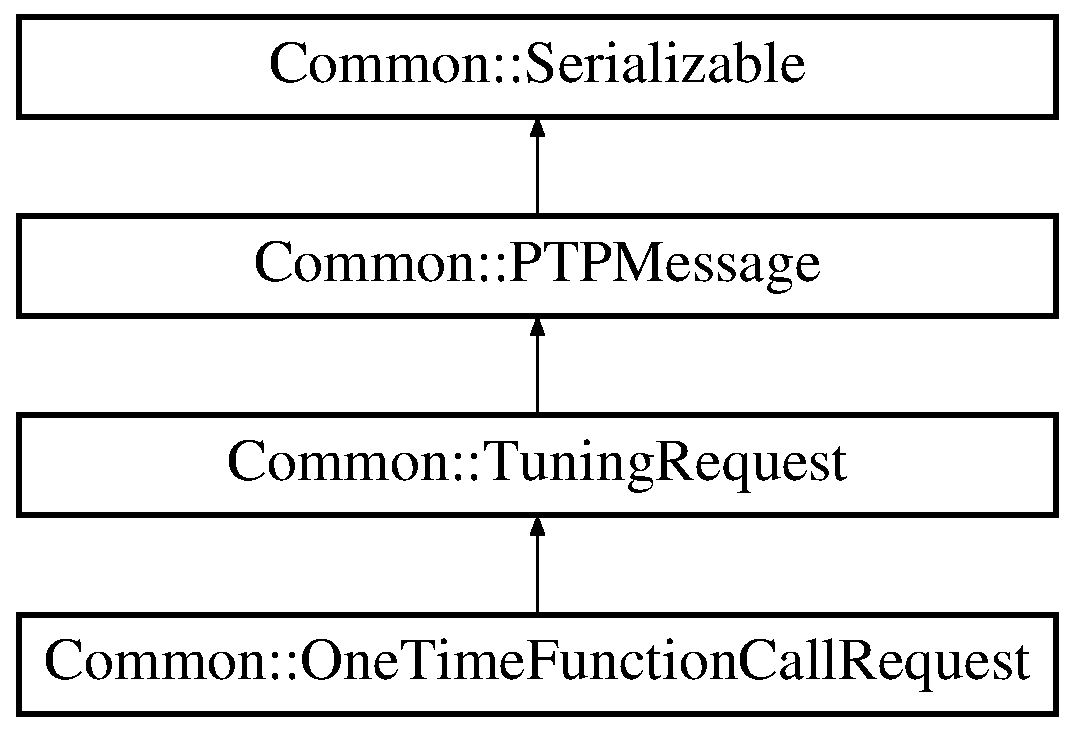
\includegraphics[height=4.000000cm]{class_common_1_1_one_time_function_call_request}
\end{center}
\end{figure}
\subsection*{Public Member Functions}
\begin{DoxyCompactItemize}
\item 
\hyperlink{class_common_1_1_one_time_function_call_request_a72c2db45188d05a5cd661d970c1734dd}{One\-Time\-Function\-Call\-Request} (int pid=0, std\-::string const \&func\-Name=std\-::string(), int n\-Attrs=0, \hyperlink{class_common_1_1_attribute}{Attribute} const $\ast$attrs=0, \hyperlink{class_common_1_1_breakpoint}{Breakpoint} const $\ast$brkpt=0)
\begin{DoxyCompactList}\small\item\em Constructor. \end{DoxyCompactList}\item 
\hypertarget{class_common_1_1_one_time_function_call_request_aee6880cf937a5a1af6027036b0a1c14d}{\hyperlink{class_common_1_1_one_time_function_call_request_aee6880cf937a5a1af6027036b0a1c14d}{$\sim$\-One\-Time\-Function\-Call\-Request} ()}\label{class_common_1_1_one_time_function_call_request_aee6880cf937a5a1af6027036b0a1c14d}

\begin{DoxyCompactList}\small\item\em Destructor. \end{DoxyCompactList}\item 
\hypertarget{class_common_1_1_one_time_function_call_request_a7c624b493dc20db48d8c6ccfc0f14693}{P\-T\-P\-Msg\-Type \hyperlink{class_common_1_1_one_time_function_call_request_a7c624b493dc20db48d8c6ccfc0f14693}{Get\-Type} () const }\label{class_common_1_1_one_time_function_call_request_a7c624b493dc20db48d8c6ccfc0f14693}

\begin{DoxyCompactList}\small\item\em Returns type of message (P\-T\-P\-One\-Time\-Func\-Call). \end{DoxyCompactList}\item 
\hypertarget{class_common_1_1_one_time_function_call_request_ad2a24593ef19e0d6efa1c7970b548427}{std\-::string const \& \hyperlink{class_common_1_1_one_time_function_call_request_ad2a24593ef19e0d6efa1c7970b548427}{Get\-Func\-Name} () const }\label{class_common_1_1_one_time_function_call_request_ad2a24593ef19e0d6efa1c7970b548427}

\begin{DoxyCompactList}\small\item\em Returns name of the function to be added. \end{DoxyCompactList}\item 
\hypertarget{class_common_1_1_one_time_function_call_request_af8640c5332f513916aa5861f0c81b6c5}{int \hyperlink{class_common_1_1_one_time_function_call_request_af8640c5332f513916aa5861f0c81b6c5}{Get\-Attr\-Count} () const }\label{class_common_1_1_one_time_function_call_request_af8640c5332f513916aa5861f0c81b6c5}

\begin{DoxyCompactList}\small\item\em Returns number of attributes the function has. \end{DoxyCompactList}\item 
\hypertarget{class_common_1_1_one_time_function_call_request_a6bea986467c6378d109aba2127fb2430}{\hyperlink{class_common_1_1_attribute}{Attribute} $\ast$ \hyperlink{class_common_1_1_one_time_function_call_request_a6bea986467c6378d109aba2127fb2430}{Get\-Attributes} () const }\label{class_common_1_1_one_time_function_call_request_a6bea986467c6378d109aba2127fb2430}

\begin{DoxyCompactList}\small\item\em Returns array of attributes. \end{DoxyCompactList}\item 
\hypertarget{class_common_1_1_one_time_function_call_request_a57294d4635ce2e919478291cc663b7af}{void \hyperlink{class_common_1_1_one_time_function_call_request_a57294d4635ce2e919478291cc663b7af}{Serialize} (\hyperlink{class_common_1_1_serializer}{Serializer} \&out) const }\label{class_common_1_1_one_time_function_call_request_a57294d4635ce2e919478291cc663b7af}

\begin{DoxyCompactList}\small\item\em Sends the message. \end{DoxyCompactList}\item 
\hypertarget{class_common_1_1_one_time_function_call_request_a92632184f0dd15656ff30cd436bc0594}{void \hyperlink{class_common_1_1_one_time_function_call_request_a92632184f0dd15656ff30cd436bc0594}{De\-Serialize} (\hyperlink{class_common_1_1_de_serializer}{De\-Serializer} \&in)}\label{class_common_1_1_one_time_function_call_request_a92632184f0dd15656ff30cd436bc0594}

\begin{DoxyCompactList}\small\item\em Gets the message. \end{DoxyCompactList}\end{DoxyCompactItemize}
\subsection*{Additional Inherited Members}


\subsection{Detailed Description}
Encapsulates a tuning request to invoke one time a given function in a given application process. 

\begin{DoxyVersion}{Version}
1.\-0b 
\end{DoxyVersion}
\begin{DoxySince}{Since}
1.\-0b 
\end{DoxySince}
\begin{DoxyAuthor}{Author}
Ania Sikora, 2003 
\end{DoxyAuthor}


\subsection{Constructor \& Destructor Documentation}
\hypertarget{class_common_1_1_one_time_function_call_request_a72c2db45188d05a5cd661d970c1734dd}{\index{Common\-::\-One\-Time\-Function\-Call\-Request@{Common\-::\-One\-Time\-Function\-Call\-Request}!One\-Time\-Function\-Call\-Request@{One\-Time\-Function\-Call\-Request}}
\index{One\-Time\-Function\-Call\-Request@{One\-Time\-Function\-Call\-Request}!Common::OneTimeFunctionCallRequest@{Common\-::\-One\-Time\-Function\-Call\-Request}}
\subsubsection[{One\-Time\-Function\-Call\-Request}]{\setlength{\rightskip}{0pt plus 5cm}Common\-::\-One\-Time\-Function\-Call\-Request\-::\-One\-Time\-Function\-Call\-Request (
\begin{DoxyParamCaption}
\item[{int}]{pid = {\ttfamily 0}, }
\item[{std\-::string const \&}]{func\-Name = {\ttfamily std\-:\-:string()}, }
\item[{int}]{n\-Attrs = {\ttfamily 0}, }
\item[{{\bf Attribute} const $\ast$}]{attrs = {\ttfamily 0}, }
\item[{{\bf Breakpoint} const $\ast$}]{brkpt = {\ttfamily 0}}
\end{DoxyParamCaption}
)\hspace{0.3cm}{\ttfamily [inline]}}}\label{class_common_1_1_one_time_function_call_request_a72c2db45188d05a5cd661d970c1734dd}


Constructor. 


\begin{DoxyParams}{Parameters}
{\em pid} & Id of the process where the call will be inserted, default 0. \\
\hline
{\em func\-Name} & Name of the function to call, default \char`\"{}\char`\"{}. \\
\hline
{\em n\-Attrs} & Number of attributes the function has, default 0. \\
\hline
{\em attrs} & \hyperlink{class_common_1_1_attribute}{Attribute} array, default 0. \\
\hline
{\em brkpt} & Used for synchronization purposes, the actual tuning will be executed when the execution reaches the breakpoint, default 0. \\
\hline
\end{DoxyParams}


The documentation for this class was generated from the following files\-:\begin{DoxyCompactItemize}
\item 
Common/P\-T\-P\-Msg.\-h\item 
Common/P\-T\-P\-Msg.\-cpp\end{DoxyCompactItemize}

\hypertarget{class_common_1_1_output_stream}{\section{Common\-:\-:Output\-Stream Class Reference}
\label{class_common_1_1_output_stream}\index{Common\-::\-Output\-Stream@{Common\-::\-Output\-Stream}}
}


Abstract class, represents an output stream of bytes.  




{\ttfamily \#include $<$Output\-Stream.\-h$>$}

Inheritance diagram for Common\-:\-:Output\-Stream\-:\begin{figure}[H]
\begin{center}
\leavevmode
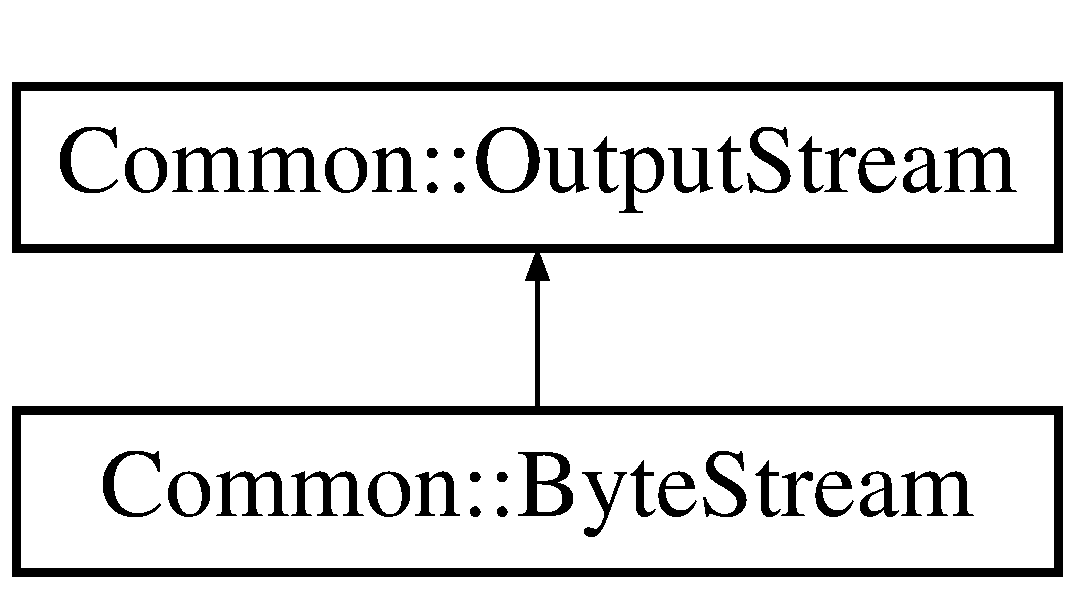
\includegraphics[height=2.000000cm]{class_common_1_1_output_stream}
\end{center}
\end{figure}
\subsection*{Public Member Functions}
\begin{DoxyCompactItemize}
\item 
\hypertarget{class_common_1_1_output_stream_a165b55bad82bdff4f0e700827187ef88}{virtual void {\bfseries Write} (char const $\ast$buf, size\-\_\-t size)=0}\label{class_common_1_1_output_stream_a165b55bad82bdff4f0e700827187ef88}

\end{DoxyCompactItemize}


\subsection{Detailed Description}
Abstract class, represents an output stream of bytes. 

This abstract class is the superclass of all classes representing an output stream of bytes. An output stream accepts output bytes and sends them to some sink.

Applications that need to define a subclass of \hyperlink{class_common_1_1_output_stream}{Output\-Stream} must always provide at least a method that writes one byte of output.

\begin{DoxyVersion}{Version}
1.\-0b 
\end{DoxyVersion}
\begin{DoxySince}{Since}
1.\-0b 
\end{DoxySince}
\begin{DoxyAuthor}{Author}
Ania Sikora, 2003 
\end{DoxyAuthor}


The documentation for this class was generated from the following file\-:\begin{DoxyCompactItemize}
\item 
Common/Output\-Stream.\-h\end{DoxyCompactItemize}

\hypertarget{class_common_1_1_pipe}{\section{Common\-:\-:Pipe Class Reference}
\label{class_common_1_1_pipe}\index{Common\-::\-Pipe@{Common\-::\-Pipe}}
}


Element used to join output and input from two processes.  




{\ttfamily \#include $<$Pipe.\-h$>$}

\subsection*{Public Member Functions}
\begin{DoxyCompactItemize}
\item 
\hyperlink{class_common_1_1_pipe_a91ddad07e89d5585b1cf27fa7860e201}{Pipe} ()
\begin{DoxyCompactList}\small\item\em Constructor. \end{DoxyCompactList}\item 
\hypertarget{class_common_1_1_pipe_af4519cc3f1f13857a724db7b2220eefa}{\hyperlink{class_common_1_1_pipe_af4519cc3f1f13857a724db7b2220eefa}{$\sim$\-Pipe} ()}\label{class_common_1_1_pipe_af4519cc3f1f13857a724db7b2220eefa}

\begin{DoxyCompactList}\small\item\em Destructor. \end{DoxyCompactList}\item 
\hypertarget{class_common_1_1_pipe_abff5b09eb4aa62f756dc5137239cc450}{bool \hyperlink{class_common_1_1_pipe_abff5b09eb4aa62f756dc5137239cc450}{Is\-Read\-Open} () const }\label{class_common_1_1_pipe_abff5b09eb4aa62f756dc5137239cc450}

\begin{DoxyCompactList}\small\item\em Returns whether the read end is open or not. \end{DoxyCompactList}\item 
\hypertarget{class_common_1_1_pipe_ab8d088b877cbaea297f6eb48fe790b46}{bool \hyperlink{class_common_1_1_pipe_ab8d088b877cbaea297f6eb48fe790b46}{Is\-Write\-Open} () const }\label{class_common_1_1_pipe_ab8d088b877cbaea297f6eb48fe790b46}

\begin{DoxyCompactList}\small\item\em Returns whether the write end is open or not. \end{DoxyCompactList}\item 
\hypertarget{class_common_1_1_pipe_a5af565c0e6f067bef9a458c54bfe22a3}{int \hyperlink{class_common_1_1_pipe_a5af565c0e6f067bef9a458c54bfe22a3}{Get\-Read} () const }\label{class_common_1_1_pipe_a5af565c0e6f067bef9a458c54bfe22a3}

\begin{DoxyCompactList}\small\item\em Returns read file descriptor. \end{DoxyCompactList}\item 
\hypertarget{class_common_1_1_pipe_a8700c04b38ae865e1b94aafee03258b7}{int \hyperlink{class_common_1_1_pipe_a8700c04b38ae865e1b94aafee03258b7}{Get\-Write} () const }\label{class_common_1_1_pipe_a8700c04b38ae865e1b94aafee03258b7}

\begin{DoxyCompactList}\small\item\em Returns write file descriptor. \end{DoxyCompactList}\item 
\hypertarget{class_common_1_1_pipe_ae03641ee676afb1b1494523262d0ef62}{void \hyperlink{class_common_1_1_pipe_ae03641ee676afb1b1494523262d0ef62}{Close\-Read} ()}\label{class_common_1_1_pipe_ae03641ee676afb1b1494523262d0ef62}

\begin{DoxyCompactList}\small\item\em Closes the read end. \end{DoxyCompactList}\item 
\hypertarget{class_common_1_1_pipe_ad04e98f2fe8628fbd35b1f2ad70590b4}{void \hyperlink{class_common_1_1_pipe_ad04e98f2fe8628fbd35b1f2ad70590b4}{Close\-Write} ()}\label{class_common_1_1_pipe_ad04e98f2fe8628fbd35b1f2ad70590b4}

\begin{DoxyCompactList}\small\item\em Closes the write end. \end{DoxyCompactList}\item 
int \hyperlink{class_common_1_1_pipe_a9aeb05035180bec14dc7251c4a4dbc1c}{Read} (char $\ast$buf, int buf\-Size)
\begin{DoxyCompactList}\small\item\em Reads from the read end and stores the content on the buffer. \end{DoxyCompactList}\item 
int \hyperlink{class_common_1_1_pipe_ae52a61f9bf69495df9dcdbdd3d4ec01d}{Write} (char const $\ast$buf, int buf\-Size)
\begin{DoxyCompactList}\small\item\em Writes the content of the buffer on the write end. \end{DoxyCompactList}\end{DoxyCompactItemize}


\subsection{Detailed Description}
Element used to join output and input from two processes. 

A pair of channels that implements a unidirectional pipe.

A pipe consists of a pair of channels\-: A writable sink channel and a readable source channel. Once some bytes are written to the sink channel these can be read from source channel in the exact order in which they were written.

Whether or not a thread writing bytes to a pipe will block until another thread reads those bytes, or some previously-\/written bytes, from the pipe is system-\/dependent and therefore unspecified. Many pipe implementations will buffer up to a certain number of bytes between the sink and source channels, but such buffering should not be assumed.

\begin{DoxyVersion}{Version}
1.\-0b 
\end{DoxyVersion}
\begin{DoxySince}{Since}
1.\-0b 
\end{DoxySince}
\begin{DoxyAuthor}{Author}
Ania Sikora, 2001 
\end{DoxyAuthor}


\subsection{Constructor \& Destructor Documentation}
\hypertarget{class_common_1_1_pipe_a91ddad07e89d5585b1cf27fa7860e201}{\index{Common\-::\-Pipe@{Common\-::\-Pipe}!Pipe@{Pipe}}
\index{Pipe@{Pipe}!Common::Pipe@{Common\-::\-Pipe}}
\subsubsection[{Pipe}]{\setlength{\rightskip}{0pt plus 5cm}Pipe\-::\-Pipe (
\begin{DoxyParamCaption}
{}
\end{DoxyParamCaption}
)}}\label{class_common_1_1_pipe_a91ddad07e89d5585b1cf27fa7860e201}


Constructor. 


\begin{DoxyExceptions}{Exceptions}
{\em \hyperlink{class_common_1_1_sys_exception}{Sys\-Exception}} & \\
\hline
\end{DoxyExceptions}


\subsection{Member Function Documentation}
\hypertarget{class_common_1_1_pipe_a9aeb05035180bec14dc7251c4a4dbc1c}{\index{Common\-::\-Pipe@{Common\-::\-Pipe}!Read@{Read}}
\index{Read@{Read}!Common::Pipe@{Common\-::\-Pipe}}
\subsubsection[{Read}]{\setlength{\rightskip}{0pt plus 5cm}int Pipe\-::\-Read (
\begin{DoxyParamCaption}
\item[{char $\ast$}]{buf, }
\item[{int}]{buf\-Size}
\end{DoxyParamCaption}
)}}\label{class_common_1_1_pipe_a9aeb05035180bec14dc7251c4a4dbc1c}


Reads from the read end and stores the content on the buffer. 


\begin{DoxyExceptions}{Exceptions}
{\em \hyperlink{class_common_1_1_sys_exception}{Sys\-Exception}} & \\
\hline
\end{DoxyExceptions}
\hypertarget{class_common_1_1_pipe_ae52a61f9bf69495df9dcdbdd3d4ec01d}{\index{Common\-::\-Pipe@{Common\-::\-Pipe}!Write@{Write}}
\index{Write@{Write}!Common::Pipe@{Common\-::\-Pipe}}
\subsubsection[{Write}]{\setlength{\rightskip}{0pt plus 5cm}int Pipe\-::\-Write (
\begin{DoxyParamCaption}
\item[{char const $\ast$}]{buf, }
\item[{int}]{buf\-Size}
\end{DoxyParamCaption}
)}}\label{class_common_1_1_pipe_ae52a61f9bf69495df9dcdbdd3d4ec01d}


Writes the content of the buffer on the write end. 


\begin{DoxyExceptions}{Exceptions}
{\em \hyperlink{class_common_1_1_sys_exception}{Sys\-Exception}} & \\
\hline
\end{DoxyExceptions}


The documentation for this class was generated from the following files\-:\begin{DoxyCompactItemize}
\item 
Common/Pipe.\-h\item 
Common/Pipe.\-cpp\end{DoxyCompactItemize}

\hypertarget{class_point_list}{\section{Point\-List Class Reference}
\label{class_point_list}\index{Point\-List@{Point\-List}}
}


Class that stores a vector of B\-Patch\-\_\-points and handles it. Can also get the address and function names of a given point.  




{\ttfamily \#include $<$di.\-h$>$}

\subsection*{Public Member Functions}
\begin{DoxyCompactItemize}
\item 
\hyperlink{class_point_list_a120d3da68f779570c3470594824aecb5}{Point\-List} (\hyperlink{class_di_function}{Di\-Function} \&func)
\begin{DoxyCompactList}\small\item\em Constructor. \end{DoxyCompactList}\item 
int \hyperlink{class_point_list_a2aeb6e16818aca9c31c8eb876d755168}{Get\-Size} () const 
\begin{DoxyCompactList}\small\item\em Getter of the vector size. \end{DoxyCompactList}\item 
void \hyperlink{class_point_list_aee028324ff3fae28e4a36856acf7f598}{Get\-Called\-Func\-Name} (B\-Patch\-\_\-point \&point, char $\ast$name, int length)
\begin{DoxyCompactList}\small\item\em Gets the name of the function called at the given point. \end{DoxyCompactList}\item 
unsigned long \hyperlink{class_point_list_a7c950aded53ab52480b235889ea5e2ba}{Get\-Address} (B\-Patch\-\_\-point \&point)
\begin{DoxyCompactList}\small\item\em Gets the address of the given point. \end{DoxyCompactList}\item 
\hypertarget{class_point_list_acf7afef0c6265b89ab42e1a12e042313}{B\-Patch\-\_\-point \& {\bfseries operator\mbox{[}$\,$\mbox{]}} (int i) const }\label{class_point_list_acf7afef0c6265b89ab42e1a12e042313}

\end{DoxyCompactItemize}


\subsection{Detailed Description}
Class that stores a vector of B\-Patch\-\_\-points and handles it. Can also get the address and function names of a given point. 

\begin{DoxyVersion}{Version}
1.\-0b 
\end{DoxyVersion}
\begin{DoxyAuthor}{Author}
Ania Sikora, 2002 
\end{DoxyAuthor}
\begin{DoxySince}{Since}
1.\-0b 
\end{DoxySince}


\subsection{Constructor \& Destructor Documentation}
\hypertarget{class_point_list_a120d3da68f779570c3470594824aecb5}{\index{Point\-List@{Point\-List}!Point\-List@{Point\-List}}
\index{Point\-List@{Point\-List}!PointList@{Point\-List}}
\subsubsection[{Point\-List}]{\setlength{\rightskip}{0pt plus 5cm}Point\-List\-::\-Point\-List (
\begin{DoxyParamCaption}
\item[{{\bf Di\-Function} \&}]{func}
\end{DoxyParamCaption}
)\hspace{0.3cm}{\ttfamily [inline]}}}\label{class_point_list_a120d3da68f779570c3470594824aecb5}


Constructor. 


\begin{DoxyParams}{Parameters}
{\em func} & \\
\hline
\end{DoxyParams}


\subsection{Member Function Documentation}
\hypertarget{class_point_list_a7c950aded53ab52480b235889ea5e2ba}{\index{Point\-List@{Point\-List}!Get\-Address@{Get\-Address}}
\index{Get\-Address@{Get\-Address}!PointList@{Point\-List}}
\subsubsection[{Get\-Address}]{\setlength{\rightskip}{0pt plus 5cm}unsigned long Point\-List\-::\-Get\-Address (
\begin{DoxyParamCaption}
\item[{B\-Patch\-\_\-point \&}]{point}
\end{DoxyParamCaption}
)\hspace{0.3cm}{\ttfamily [inline]}}}\label{class_point_list_a7c950aded53ab52480b235889ea5e2ba}


Gets the address of the given point. 


\begin{DoxyParams}{Parameters}
{\em point} & Given point to look get address from \\
\hline
\end{DoxyParams}
\begin{DoxyReturn}{Returns}
Address of the given point 
\end{DoxyReturn}
\hypertarget{class_point_list_aee028324ff3fae28e4a36856acf7f598}{\index{Point\-List@{Point\-List}!Get\-Called\-Func\-Name@{Get\-Called\-Func\-Name}}
\index{Get\-Called\-Func\-Name@{Get\-Called\-Func\-Name}!PointList@{Point\-List}}
\subsubsection[{Get\-Called\-Func\-Name}]{\setlength{\rightskip}{0pt plus 5cm}void Point\-List\-::\-Get\-Called\-Func\-Name (
\begin{DoxyParamCaption}
\item[{B\-Patch\-\_\-point \&}]{point, }
\item[{char $\ast$}]{name, }
\item[{int}]{length}
\end{DoxyParamCaption}
)\hspace{0.3cm}{\ttfamily [inline]}}}\label{class_point_list_aee028324ff3fae28e4a36856acf7f598}


Gets the name of the function called at the given point. 


\begin{DoxyParams}{Parameters}
{\em point} & Point where the function is \\
\hline
{\em name} & Name of the function \\
\hline
{\em length} & Length of the name \\
\hline
\end{DoxyParams}
\hypertarget{class_point_list_a2aeb6e16818aca9c31c8eb876d755168}{\index{Point\-List@{Point\-List}!Get\-Size@{Get\-Size}}
\index{Get\-Size@{Get\-Size}!PointList@{Point\-List}}
\subsubsection[{Get\-Size}]{\setlength{\rightskip}{0pt plus 5cm}int Point\-List\-::\-Get\-Size (
\begin{DoxyParamCaption}
{}
\end{DoxyParamCaption}
) const\hspace{0.3cm}{\ttfamily [inline]}}}\label{class_point_list_a2aeb6e16818aca9c31c8eb876d755168}


Getter of the vector size. 

\begin{DoxyReturn}{Returns}
Vector's size 
\end{DoxyReturn}


The documentation for this class was generated from the following file\-:\begin{DoxyCompactItemize}
\item 
Common/di.\-h\end{DoxyCompactItemize}

\hypertarget{class_procedure_list}{\section{Procedure\-List Class Reference}
\label{class_procedure_list}\index{Procedure\-List@{Procedure\-List}}
}


Implements and handles a vector of B\-Patch\-\_\-functions.  




{\ttfamily \#include $<$di.\-h$>$}

\subsection*{Public Member Functions}
\begin{DoxyCompactItemize}
\item 
\hyperlink{class_procedure_list_a21b30b5349812a669625177fb7efc224}{Procedure\-List} (B\-Patch\-\_\-image \&bp\-Image)
\begin{DoxyCompactList}\small\item\em Constructor. \end{DoxyCompactList}\item 
int \hyperlink{class_procedure_list_a0b3c110b1b4c1f15968c618a10a3c82c}{Get\-Size} () const 
\begin{DoxyCompactList}\small\item\em Getter of the vector's size. \end{DoxyCompactList}\item 
\hypertarget{class_procedure_list_a73da6b29354ed6d011e0f31ec7e48d5d}{B\-Patch\-\_\-function \& {\bfseries operator\mbox{[}$\,$\mbox{]}} (int i) const }\label{class_procedure_list_a73da6b29354ed6d011e0f31ec7e48d5d}

\end{DoxyCompactItemize}


\subsection{Detailed Description}
Implements and handles a vector of B\-Patch\-\_\-functions. 

\begin{DoxyVersion}{Version}
1.\-0b 
\end{DoxyVersion}
\begin{DoxyAuthor}{Author}
Ania Sikora, 2002 
\end{DoxyAuthor}
\begin{DoxySince}{Since}
1.\-0b 
\end{DoxySince}


\subsection{Constructor \& Destructor Documentation}
\hypertarget{class_procedure_list_a21b30b5349812a669625177fb7efc224}{\index{Procedure\-List@{Procedure\-List}!Procedure\-List@{Procedure\-List}}
\index{Procedure\-List@{Procedure\-List}!ProcedureList@{Procedure\-List}}
\subsubsection[{Procedure\-List}]{\setlength{\rightskip}{0pt plus 5cm}Procedure\-List\-::\-Procedure\-List (
\begin{DoxyParamCaption}
\item[{B\-Patch\-\_\-image \&}]{bp\-Image}
\end{DoxyParamCaption}
)\hspace{0.3cm}{\ttfamily [inline]}}}\label{class_procedure_list_a21b30b5349812a669625177fb7efc224}


Constructor. 


\begin{DoxyParams}{Parameters}
{\em bp\-Image} & Image of the program \\
\hline
\end{DoxyParams}


\subsection{Member Function Documentation}
\hypertarget{class_procedure_list_a0b3c110b1b4c1f15968c618a10a3c82c}{\index{Procedure\-List@{Procedure\-List}!Get\-Size@{Get\-Size}}
\index{Get\-Size@{Get\-Size}!ProcedureList@{Procedure\-List}}
\subsubsection[{Get\-Size}]{\setlength{\rightskip}{0pt plus 5cm}int Procedure\-List\-::\-Get\-Size (
\begin{DoxyParamCaption}
{}
\end{DoxyParamCaption}
) const\hspace{0.3cm}{\ttfamily [inline]}}}\label{class_procedure_list_a0b3c110b1b4c1f15968c618a10a3c82c}


Getter of the vector's size. 

\begin{DoxyReturn}{Returns}
Vector's size 
\end{DoxyReturn}


The documentation for this class was generated from the following file\-:\begin{DoxyCompactItemize}
\item 
Common/di.\-h\end{DoxyCompactItemize}

\hypertarget{class_common_1_1_process}{\section{Common\-:\-:Process Class Reference}
\label{class_common_1_1_process}\index{Common\-::\-Process@{Common\-::\-Process}}
}


Abstract class, creates a new process to perform different operations on the overrided method Run().  




{\ttfamily \#include $<$Process.\-h$>$}

Inheritance diagram for Common\-:\-:Process\-:\begin{figure}[H]
\begin{center}
\leavevmode
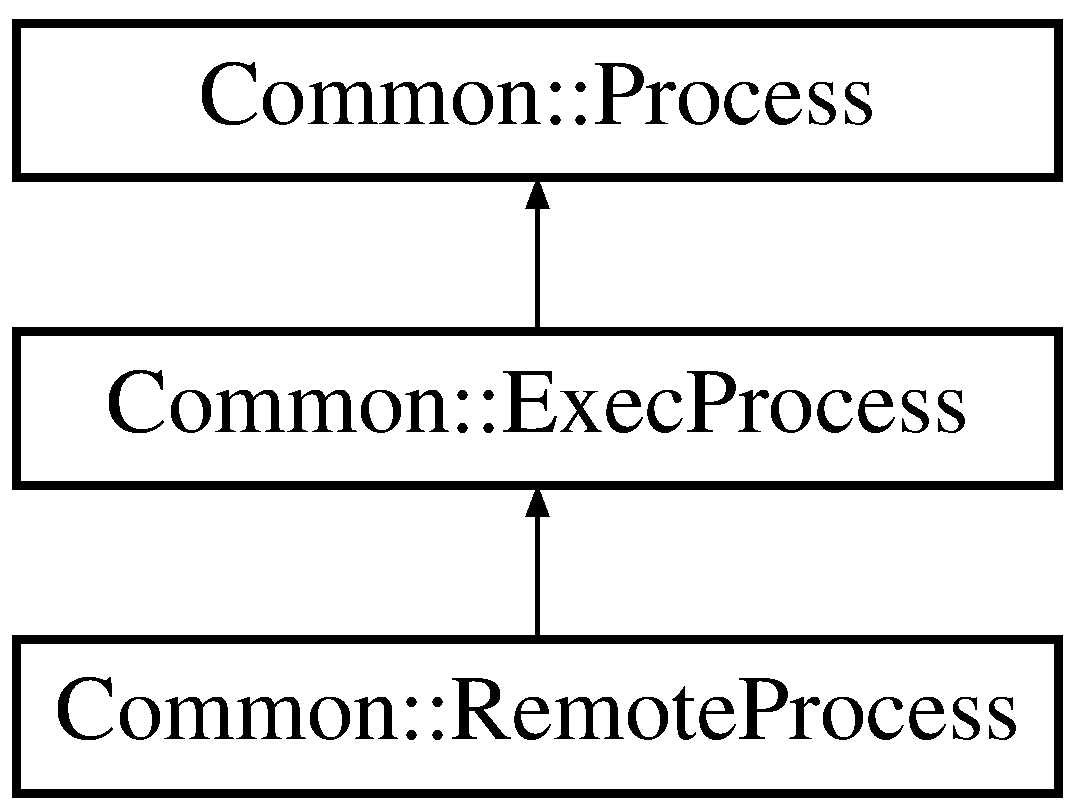
\includegraphics[height=3.000000cm]{class_common_1_1_process}
\end{center}
\end{figure}
\subsection*{Public Member Functions}
\begin{DoxyCompactItemize}
\item 
\hypertarget{class_common_1_1_process_ae92f973fc379f7020f29d08288685c33}{virtual void \hyperlink{class_common_1_1_process_ae92f973fc379f7020f29d08288685c33}{Start} ()}\label{class_common_1_1_process_ae92f973fc379f7020f29d08288685c33}

\begin{DoxyCompactList}\small\item\em Executes the process. \end{DoxyCompactList}\item 
\hypertarget{class_common_1_1_process_a6e99fb060fb742c7779255cff25dbf97}{int \hyperlink{class_common_1_1_process_a6e99fb060fb742c7779255cff25dbf97}{Get\-Pid} () const }\label{class_common_1_1_process_a6e99fb060fb742c7779255cff25dbf97}

\begin{DoxyCompactList}\small\item\em Returns process id. \end{DoxyCompactList}\end{DoxyCompactItemize}
\subsection*{Protected Member Functions}
\begin{DoxyCompactItemize}
\item 
\hypertarget{class_common_1_1_process_ab7bd6318e6828ba84639c94dca871959}{\hyperlink{class_common_1_1_process_ab7bd6318e6828ba84639c94dca871959}{Process} ()}\label{class_common_1_1_process_ab7bd6318e6828ba84639c94dca871959}

\begin{DoxyCompactList}\small\item\em Constructor. \end{DoxyCompactList}\item 
\hypertarget{class_common_1_1_process_a1d4cb970f44c0652afa6536ca5ccf4f1}{virtual int {\bfseries Run} ()=0}\label{class_common_1_1_process_a1d4cb970f44c0652afa6536ca5ccf4f1}

\end{DoxyCompactItemize}
\subsection*{Protected Attributes}
\begin{DoxyCompactItemize}
\item 
\hypertarget{class_common_1_1_process_a857c5dd43f0febae07fec9e849a5b881}{int {\bfseries \-\_\-pid}}\label{class_common_1_1_process_a857c5dd43f0febae07fec9e849a5b881}

\end{DoxyCompactItemize}


\subsection{Detailed Description}
Abstract class, creates a new process to perform different operations on the overrided method Run(). 

\begin{DoxyVersion}{Version}
1.\-0b 
\end{DoxyVersion}
\begin{DoxySince}{Since}
1.\-0b 
\end{DoxySince}
\begin{DoxyAuthor}{Author}
Ania Sikora, 2001 
\end{DoxyAuthor}


The documentation for this class was generated from the following files\-:\begin{DoxyCompactItemize}
\item 
Common/Process.\-h\item 
Common/Process.\-cpp\end{DoxyCompactItemize}

\hypertarget{class_p_t_p_acceptor}{\section{P\-T\-P\-Acceptor Class Reference}
\label{class_p_t_p_acceptor}\index{P\-T\-P\-Acceptor@{P\-T\-P\-Acceptor}}
}


Manages socket connection and handles data input through them.  




{\ttfamily \#include $<$P\-T\-P\-Acceptor.\-h$>$}

Inheritance diagram for P\-T\-P\-Acceptor\-:\begin{figure}[H]
\begin{center}
\leavevmode
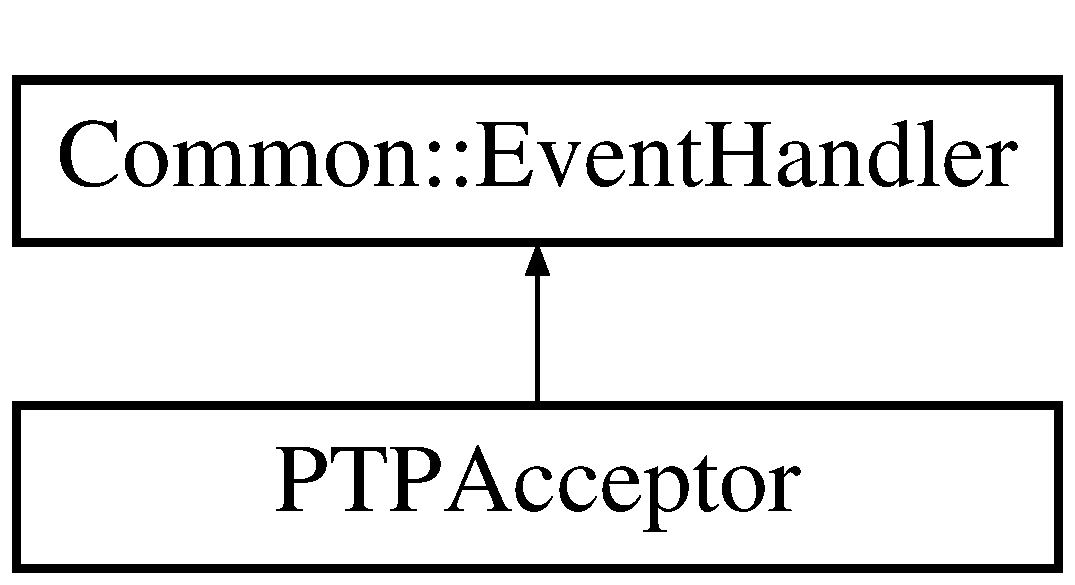
\includegraphics[height=2.000000cm]{class_p_t_p_acceptor}
\end{center}
\end{figure}
\subsection*{Public Member Functions}
\begin{DoxyCompactItemize}
\item 
\hyperlink{class_p_t_p_acceptor_a2886d7acd766d591b94b61063e4b6348}{P\-T\-P\-Acceptor} (\hyperlink{class_common_1_1_reactor}{Reactor} \&reactor, \hyperlink{class_task_manager}{Task\-Manager} \&tm, int port)
\begin{DoxyCompactList}\small\item\em Constructor. \end{DoxyCompactList}\item 
\hypertarget{class_p_t_p_acceptor_abfff4da1e33e6957e8a349bd8671a342}{\hyperlink{class_p_t_p_acceptor_abfff4da1e33e6957e8a349bd8671a342}{$\sim$\-P\-T\-P\-Acceptor} ()}\label{class_p_t_p_acceptor_abfff4da1e33e6957e8a349bd8671a342}

\begin{DoxyCompactList}\small\item\em Destructor. \end{DoxyCompactList}\item 
\hypertarget{class_p_t_p_acceptor_a3c280f3a20cd06fe94d72d6a715d9ebe}{void \hyperlink{class_p_t_p_acceptor_a3c280f3a20cd06fe94d72d6a715d9ebe}{Handle\-Input} ()}\label{class_p_t_p_acceptor_a3c280f3a20cd06fe94d72d6a715d9ebe}

\begin{DoxyCompactList}\small\item\em Gets the socket for the client and binds it with the task manager. \end{DoxyCompactList}\item 
int \hyperlink{class_p_t_p_acceptor_abbe21f4a532eb23a96ea696f7b344a32}{Get\-Handle} ()
\begin{DoxyCompactList}\small\item\em Getter of a handler for the variable \-\_\-socket. \end{DoxyCompactList}\end{DoxyCompactItemize}


\subsection{Detailed Description}
Manages socket connection and handles data input through them. 

\begin{DoxyVersion}{Version}
1.\-0 
\end{DoxyVersion}
\begin{DoxySince}{Since}
1.\-0 
\end{DoxySince}
\begin{DoxyAuthor}{Author}
Ania Sikora, 2002 
\end{DoxyAuthor}


\subsection{Constructor \& Destructor Documentation}
\hypertarget{class_p_t_p_acceptor_a2886d7acd766d591b94b61063e4b6348}{\index{P\-T\-P\-Acceptor@{P\-T\-P\-Acceptor}!P\-T\-P\-Acceptor@{P\-T\-P\-Acceptor}}
\index{P\-T\-P\-Acceptor@{P\-T\-P\-Acceptor}!PTPAcceptor@{P\-T\-P\-Acceptor}}
\subsubsection[{P\-T\-P\-Acceptor}]{\setlength{\rightskip}{0pt plus 5cm}P\-T\-P\-Acceptor\-::\-P\-T\-P\-Acceptor (
\begin{DoxyParamCaption}
\item[{{\bf Reactor} \&}]{reactor, }
\item[{{\bf Task\-Manager} \&}]{tm, }
\item[{int}]{port}
\end{DoxyParamCaption}
)}}\label{class_p_t_p_acceptor_a2886d7acd766d591b94b61063e4b6348}


Constructor. 


\begin{DoxyParams}{Parameters}
{\em reactor} & Object of class reactor that manages event handlers. \\
\hline
{\em tm} & \hyperlink{class_task}{Task} manager. \\
\hline
\end{DoxyParams}


\subsection{Member Function Documentation}
\hypertarget{class_p_t_p_acceptor_abbe21f4a532eb23a96ea696f7b344a32}{\index{P\-T\-P\-Acceptor@{P\-T\-P\-Acceptor}!Get\-Handle@{Get\-Handle}}
\index{Get\-Handle@{Get\-Handle}!PTPAcceptor@{P\-T\-P\-Acceptor}}
\subsubsection[{Get\-Handle}]{\setlength{\rightskip}{0pt plus 5cm}int P\-T\-P\-Acceptor\-::\-Get\-Handle (
\begin{DoxyParamCaption}
{}
\end{DoxyParamCaption}
)\hspace{0.3cm}{\ttfamily [inline]}, {\ttfamily [virtual]}}}\label{class_p_t_p_acceptor_abbe21f4a532eb23a96ea696f7b344a32}


Getter of a handler for the variable \-\_\-socket. 

\begin{DoxyReturn}{Returns}
Handle of the server socket. 
\end{DoxyReturn}


Implements \hyperlink{class_common_1_1_event_handler_aaf6cb56038c6fe6b91c9d1e34ee6b3af}{Common\-::\-Event\-Handler}.



The documentation for this class was generated from the following files\-:\begin{DoxyCompactItemize}
\item 
A\-C/P\-T\-P\-Acceptor.\-h\item 
A\-C/P\-T\-P\-Acceptor.\-cpp\end{DoxyCompactItemize}

\hypertarget{class_p_t_p_handler}{\section{P\-T\-P\-Handler Class Reference}
\label{class_p_t_p_handler}\index{P\-T\-P\-Handler@{P\-T\-P\-Handler}}
}


Manages the requests from the \hyperlink{class_p_t_p_acceptor}{P\-T\-P\-Acceptor}.  




{\ttfamily \#include $<$P\-T\-P\-Handler.\-h$>$}

Inheritance diagram for P\-T\-P\-Handler\-:\begin{figure}[H]
\begin{center}
\leavevmode
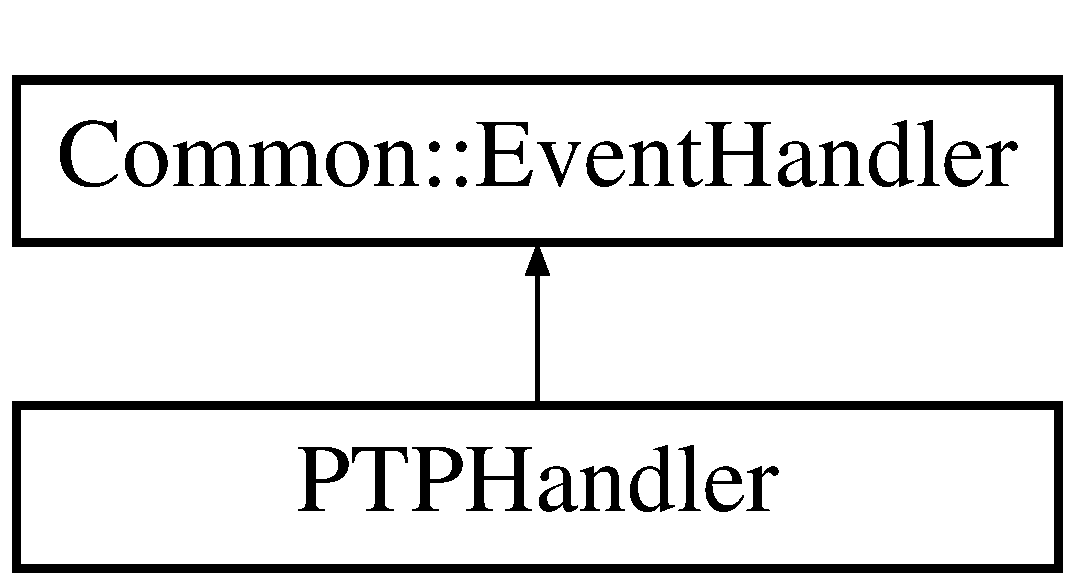
\includegraphics[height=2.000000cm]{class_p_t_p_handler}
\end{center}
\end{figure}
\subsection*{Public Member Functions}
\begin{DoxyCompactItemize}
\item 
\hyperlink{class_p_t_p_handler_a8822999ece7959f308a744a8e2f9820b}{P\-T\-P\-Handler} (Socket\-Ptr \&socket, \hyperlink{class_task_manager}{Task\-Manager} \&tm)
\begin{DoxyCompactList}\small\item\em Constructor. \end{DoxyCompactList}\item 
\hypertarget{class_p_t_p_handler_a7e5a0b3cbf3a55ead9e35d5303d58288}{void \hyperlink{class_p_t_p_handler_a7e5a0b3cbf3a55ead9e35d5303d58288}{Handle\-Input} ()}\label{class_p_t_p_handler_a7e5a0b3cbf3a55ead9e35d5303d58288}

\begin{DoxyCompactList}\small\item\em Reads message from socket and handles the different kinds of requests that are received. \end{DoxyCompactList}\item 
int \hyperlink{class_p_t_p_handler_a88a9be1a38bfc1f434eaac10984dc9a0}{Get\-Handle} ()
\begin{DoxyCompactList}\small\item\em Getter of a handler for the variable \-\_\-socket. \end{DoxyCompactList}\end{DoxyCompactItemize}


\subsection{Detailed Description}
Manages the requests from the \hyperlink{class_p_t_p_acceptor}{P\-T\-P\-Acceptor}. 

\begin{DoxyVersion}{Version}
1.\-0 
\end{DoxyVersion}
\begin{DoxySince}{Since}
1.\-0 
\end{DoxySince}
\begin{DoxyAuthor}{Author}
Ania Sikora, 2002 
\end{DoxyAuthor}


\subsection{Constructor \& Destructor Documentation}
\hypertarget{class_p_t_p_handler_a8822999ece7959f308a744a8e2f9820b}{\index{P\-T\-P\-Handler@{P\-T\-P\-Handler}!P\-T\-P\-Handler@{P\-T\-P\-Handler}}
\index{P\-T\-P\-Handler@{P\-T\-P\-Handler}!PTPHandler@{P\-T\-P\-Handler}}
\subsubsection[{P\-T\-P\-Handler}]{\setlength{\rightskip}{0pt plus 5cm}P\-T\-P\-Handler\-::\-P\-T\-P\-Handler (
\begin{DoxyParamCaption}
\item[{Socket\-Ptr \&}]{socket, }
\item[{{\bf Task\-Manager} \&}]{tm}
\end{DoxyParamCaption}
)\hspace{0.3cm}{\ttfamily [inline]}}}\label{class_p_t_p_handler_a8822999ece7959f308a744a8e2f9820b}


Constructor. 


\begin{DoxyParams}{Parameters}
{\em socket} & Pointer to the socket used to get the input (request). \\
\hline
{\em tm} & \hyperlink{class_task}{Task} manager that handles the task to which the request affects. \\
\hline
\end{DoxyParams}


\subsection{Member Function Documentation}
\hypertarget{class_p_t_p_handler_a88a9be1a38bfc1f434eaac10984dc9a0}{\index{P\-T\-P\-Handler@{P\-T\-P\-Handler}!Get\-Handle@{Get\-Handle}}
\index{Get\-Handle@{Get\-Handle}!PTPHandler@{P\-T\-P\-Handler}}
\subsubsection[{Get\-Handle}]{\setlength{\rightskip}{0pt plus 5cm}int P\-T\-P\-Handler\-::\-Get\-Handle (
\begin{DoxyParamCaption}
{}
\end{DoxyParamCaption}
)\hspace{0.3cm}{\ttfamily [inline]}, {\ttfamily [virtual]}}}\label{class_p_t_p_handler_a88a9be1a38bfc1f434eaac10984dc9a0}


Getter of a handler for the variable \-\_\-socket. 

\begin{DoxyReturn}{Returns}
Handle of the socket. 
\end{DoxyReturn}


Implements \hyperlink{class_common_1_1_event_handler_aaf6cb56038c6fe6b91c9d1e34ee6b3af}{Common\-::\-Event\-Handler}.



The documentation for this class was generated from the following files\-:\begin{DoxyCompactItemize}
\item 
A\-C/P\-T\-P\-Handler.\-h\item 
A\-C/P\-T\-P\-Handler.\-cpp\end{DoxyCompactItemize}

\hypertarget{class_common_1_1_p_t_p_message}{\section{Common\-:\-:P\-T\-P\-Message Class Reference}
\label{class_common_1_1_p_t_p_message}\index{Common\-::\-P\-T\-P\-Message@{Common\-::\-P\-T\-P\-Message}}
}


Performance tuning protocol, represents a message interchanged between analyzer and tuner/tracer.  




{\ttfamily \#include $<$P\-T\-P\-Msg.\-h$>$}

Inheritance diagram for Common\-:\-:P\-T\-P\-Message\-:\begin{figure}[H]
\begin{center}
\leavevmode
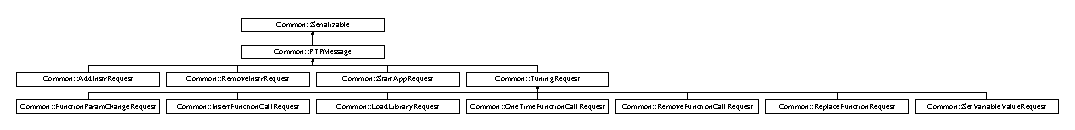
\includegraphics[height=1.295547cm]{class_common_1_1_p_t_p_message}
\end{center}
\end{figure}
\subsection*{Public Member Functions}
\begin{DoxyCompactItemize}
\item 
\hypertarget{class_common_1_1_p_t_p_message_a1a7568792ffddbe05beba780dc13d608}{\hyperlink{class_common_1_1_p_t_p_message_a1a7568792ffddbe05beba780dc13d608}{P\-T\-P\-Message} ()}\label{class_common_1_1_p_t_p_message_a1a7568792ffddbe05beba780dc13d608}

\begin{DoxyCompactList}\small\item\em Constructor. \end{DoxyCompactList}\item 
\hypertarget{class_common_1_1_p_t_p_message_a0400ff9945ee7f33ddc15baf25771997}{virtual P\-T\-P\-Msg\-Type \hyperlink{class_common_1_1_p_t_p_message_a0400ff9945ee7f33ddc15baf25771997}{Get\-Type} () const }\label{class_common_1_1_p_t_p_message_a0400ff9945ee7f33ddc15baf25771997}

\begin{DoxyCompactList}\small\item\em To be implemented by subclasses. \end{DoxyCompactList}\item 
\hypertarget{class_common_1_1_p_t_p_message_acfbc6798267f71ee93eea878d201973a}{int \hyperlink{class_common_1_1_p_t_p_message_acfbc6798267f71ee93eea878d201973a}{Get\-Data\-Size} () const }\label{class_common_1_1_p_t_p_message_acfbc6798267f71ee93eea878d201973a}

\begin{DoxyCompactList}\small\item\em Returns size of the data once serialized. \end{DoxyCompactList}\item 
\hypertarget{class_common_1_1_p_t_p_message_ad864518e8c0dc31c38a926909c6fb85e}{virtual \hyperlink{class_common_1_1_p_t_p_message_ad864518e8c0dc31c38a926909c6fb85e}{$\sim$\-P\-T\-P\-Message} ()}\label{class_common_1_1_p_t_p_message_ad864518e8c0dc31c38a926909c6fb85e}

\begin{DoxyCompactList}\small\item\em Destructor. \end{DoxyCompactList}\end{DoxyCompactItemize}


\subsection{Detailed Description}
Performance tuning protocol, represents a message interchanged between analyzer and tuner/tracer. 

\begin{DoxyVersion}{Version}
1.\-0b 
\end{DoxyVersion}
\begin{DoxySince}{Since}
1.\-0b 
\end{DoxySince}
\begin{DoxyAuthor}{Author}
Ania Sikora, 2003 
\end{DoxyAuthor}


The documentation for this class was generated from the following files\-:\begin{DoxyCompactItemize}
\item 
Common/P\-T\-P\-Msg.\-h\item 
Common/P\-T\-P\-Msg.\-cpp\end{DoxyCompactItemize}

\hypertarget{class_common_1_1_p_t_p_msg_header}{\section{Common\-:\-:P\-T\-P\-Msg\-Header Class Reference}
\label{class_common_1_1_p_t_p_msg_header}\index{Common\-::\-P\-T\-P\-Msg\-Header@{Common\-::\-P\-T\-P\-Msg\-Header}}
}


Represents header of a \hyperlink{class_common_1_1_p_t_p_message}{P\-T\-P\-Message} object.  




{\ttfamily \#include $<$P\-T\-P\-Msg\-Header.\-h$>$}

Inheritance diagram for Common\-:\-:P\-T\-P\-Msg\-Header\-:\begin{figure}[H]
\begin{center}
\leavevmode
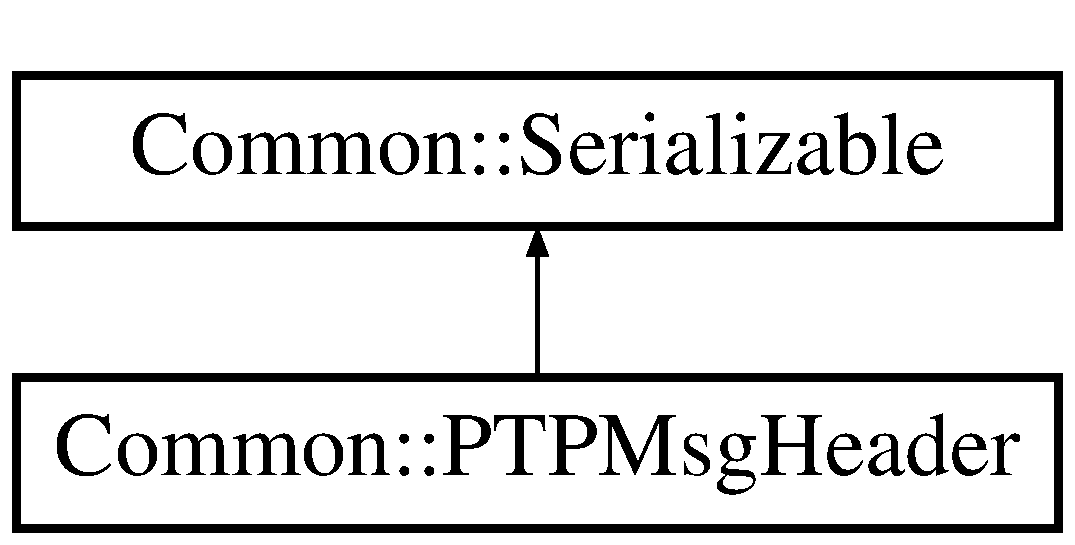
\includegraphics[height=2.000000cm]{class_common_1_1_p_t_p_msg_header}
\end{center}
\end{figure}
\subsection*{Public Member Functions}
\begin{DoxyCompactItemize}
\item 
\hypertarget{class_common_1_1_p_t_p_msg_header_a8e462bd4d4e7f337d11ce6bde2ab21af}{\hyperlink{class_common_1_1_p_t_p_msg_header_a8e462bd4d4e7f337d11ce6bde2ab21af}{P\-T\-P\-Msg\-Header} ()}\label{class_common_1_1_p_t_p_msg_header_a8e462bd4d4e7f337d11ce6bde2ab21af}

\begin{DoxyCompactList}\small\item\em Constructor. \end{DoxyCompactList}\item 
\hypertarget{class_common_1_1_p_t_p_msg_header_a4da3b559025cac427ae10171df35e565}{void \hyperlink{class_common_1_1_p_t_p_msg_header_a4da3b559025cac427ae10171df35e565}{Serialize} (\hyperlink{class_common_1_1_serializer}{Serializer} \&out) const }\label{class_common_1_1_p_t_p_msg_header_a4da3b559025cac427ae10171df35e565}

\begin{DoxyCompactList}\small\item\em Sends the message header. \end{DoxyCompactList}\item 
\hypertarget{class_common_1_1_p_t_p_msg_header_a3e83b41befc2b74efc829d676387e42e}{void \hyperlink{class_common_1_1_p_t_p_msg_header_a3e83b41befc2b74efc829d676387e42e}{De\-Serialize} (\hyperlink{class_common_1_1_de_serializer}{De\-Serializer} \&in)}\label{class_common_1_1_p_t_p_msg_header_a3e83b41befc2b74efc829d676387e42e}

\begin{DoxyCompactList}\small\item\em Receives the message header. \end{DoxyCompactList}\item 
\hypertarget{class_common_1_1_p_t_p_msg_header_a51dff8298e5ce6622fe29f2d4d7b2d38}{int \hyperlink{class_common_1_1_p_t_p_msg_header_a51dff8298e5ce6622fe29f2d4d7b2d38}{Get\-Magic} () const }\label{class_common_1_1_p_t_p_msg_header_a51dff8298e5ce6622fe29f2d4d7b2d38}

\begin{DoxyCompactList}\small\item\em Returns magic attribute. \end{DoxyCompactList}\item 
\hypertarget{class_common_1_1_p_t_p_msg_header_a96d687830243b5e736372343e1039bf1}{int \hyperlink{class_common_1_1_p_t_p_msg_header_a96d687830243b5e736372343e1039bf1}{Get\-Version} () const }\label{class_common_1_1_p_t_p_msg_header_a96d687830243b5e736372343e1039bf1}

\begin{DoxyCompactList}\small\item\em Returns version attribute. \end{DoxyCompactList}\item 
\hypertarget{class_common_1_1_p_t_p_msg_header_abd4e4d88d8e331208f39a84615f2eced}{P\-T\-P\-Msg\-Type \hyperlink{class_common_1_1_p_t_p_msg_header_abd4e4d88d8e331208f39a84615f2eced}{Get\-Type} () const }\label{class_common_1_1_p_t_p_msg_header_abd4e4d88d8e331208f39a84615f2eced}

\begin{DoxyCompactList}\small\item\em Returns the type of the message. \end{DoxyCompactList}\item 
\hypertarget{class_common_1_1_p_t_p_msg_header_a4a5e7a55146031041ff1a5013db2e4df}{int \hyperlink{class_common_1_1_p_t_p_msg_header_a4a5e7a55146031041ff1a5013db2e4df}{Get\-Data\-Size} () const }\label{class_common_1_1_p_t_p_msg_header_a4a5e7a55146031041ff1a5013db2e4df}

\begin{DoxyCompactList}\small\item\em Returns data size. \end{DoxyCompactList}\item 
\hypertarget{class_common_1_1_p_t_p_msg_header_a3cb5cb90b4d3720994df088b6d6808c6}{int \hyperlink{class_common_1_1_p_t_p_msg_header_a3cb5cb90b4d3720994df088b6d6808c6}{Get\-Header\-Size} () const }\label{class_common_1_1_p_t_p_msg_header_a3cb5cb90b4d3720994df088b6d6808c6}

\begin{DoxyCompactList}\small\item\em Returns header size. \end{DoxyCompactList}\item 
\hypertarget{class_common_1_1_p_t_p_msg_header_a8496dde4a8ed05f8eb2b69041c52419f}{void \hyperlink{class_common_1_1_p_t_p_msg_header_a8496dde4a8ed05f8eb2b69041c52419f}{Set\-Magic} (int magic)}\label{class_common_1_1_p_t_p_msg_header_a8496dde4a8ed05f8eb2b69041c52419f}

\begin{DoxyCompactList}\small\item\em Sets the magic attribute. \end{DoxyCompactList}\item 
\hypertarget{class_common_1_1_p_t_p_msg_header_a10fbb2b5fecd8966b38b407f27e23800}{void \hyperlink{class_common_1_1_p_t_p_msg_header_a10fbb2b5fecd8966b38b407f27e23800}{Set\-Version} (int version)}\label{class_common_1_1_p_t_p_msg_header_a10fbb2b5fecd8966b38b407f27e23800}

\begin{DoxyCompactList}\small\item\em Sets the version attribute. \end{DoxyCompactList}\item 
\hypertarget{class_common_1_1_p_t_p_msg_header_a58c7cee7c62009708b434779ab4324d6}{void \hyperlink{class_common_1_1_p_t_p_msg_header_a58c7cee7c62009708b434779ab4324d6}{Set\-Msg\-Type} (P\-T\-P\-Msg\-Type type)}\label{class_common_1_1_p_t_p_msg_header_a58c7cee7c62009708b434779ab4324d6}

\begin{DoxyCompactList}\small\item\em Sets the type of the message. \end{DoxyCompactList}\item 
\hypertarget{class_common_1_1_p_t_p_msg_header_aa87797fce32bafab7600a848eb6c5156}{void \hyperlink{class_common_1_1_p_t_p_msg_header_aa87797fce32bafab7600a848eb6c5156}{Set\-Data\-Size} (int size)}\label{class_common_1_1_p_t_p_msg_header_aa87797fce32bafab7600a848eb6c5156}

\begin{DoxyCompactList}\small\item\em Sets data size. \end{DoxyCompactList}\item 
\hypertarget{class_common_1_1_p_t_p_msg_header_a43c32c543abe16528f1398a4a1c21f8f}{void \hyperlink{class_common_1_1_p_t_p_msg_header_a43c32c543abe16528f1398a4a1c21f8f}{Set\-Header\-Size} ()}\label{class_common_1_1_p_t_p_msg_header_a43c32c543abe16528f1398a4a1c21f8f}

\begin{DoxyCompactList}\small\item\em Updates header size. \end{DoxyCompactList}\end{DoxyCompactItemize}


\subsection{Detailed Description}
Represents header of a \hyperlink{class_common_1_1_p_t_p_message}{P\-T\-P\-Message} object. 

\begin{DoxyVersion}{Version}
1.\-0b 
\end{DoxyVersion}
\begin{DoxySince}{Since}
1.\-0b 
\end{DoxySince}
\begin{DoxyAuthor}{Author}
Ania Sikora, 2002 
\end{DoxyAuthor}


The documentation for this class was generated from the following files\-:\begin{DoxyCompactItemize}
\item 
Common/P\-T\-P\-Msg\-Header.\-h\item 
Common/P\-T\-P\-Msg\-Header.\-cpp\end{DoxyCompactItemize}

\hypertarget{class_common_1_1_p_t_p_protocol}{\section{Common\-:\-:P\-T\-P\-Protocol Class Reference}
\label{class_common_1_1_p_t_p_protocol}\index{Common\-::\-P\-T\-P\-Protocol@{Common\-::\-P\-T\-P\-Protocol}}
}


Communicates analyzer and tuner.  




{\ttfamily \#include $<$P\-T\-P\-Protocol.\-h$>$}

\subsection*{Static Public Member Functions}
\begin{DoxyCompactItemize}
\item 
\hypertarget{class_common_1_1_p_t_p_protocol_abd98607c51b2934bbbad21d899f2b460}{static void \hyperlink{class_common_1_1_p_t_p_protocol_abd98607c51b2934bbbad21d899f2b460}{Write\-Message} (\hyperlink{class_common_1_1_p_t_p_message}{P\-T\-P\-Message} \&msg, \hyperlink{class_common_1_1_output_stream}{Output\-Stream} \&stream)}\label{class_common_1_1_p_t_p_protocol_abd98607c51b2934bbbad21d899f2b460}

\begin{DoxyCompactList}\small\item\em Sends a message through a stream to the tuner. \end{DoxyCompactList}\item 
\hypertarget{class_common_1_1_p_t_p_protocol_a075f252ac5dd290fc0f372224c1097b4}{static \hyperlink{class_common_1_1_p_t_p_message}{P\-T\-P\-Message} $\ast$ \hyperlink{class_common_1_1_p_t_p_protocol_a075f252ac5dd290fc0f372224c1097b4}{Read\-Message} (std\-::istream \&stream)}\label{class_common_1_1_p_t_p_protocol_a075f252ac5dd290fc0f372224c1097b4}

\begin{DoxyCompactList}\small\item\em Receives a message through a stream from the analyzer. \end{DoxyCompactList}\item 
\hypertarget{class_common_1_1_p_t_p_protocol_acc152836fd36e641e964fea44b5b1064}{static void \hyperlink{class_common_1_1_p_t_p_protocol_acc152836fd36e641e964fea44b5b1064}{Write\-Message\-Ex} (\hyperlink{class_common_1_1_p_t_p_message}{P\-T\-P\-Message} \&msg, \hyperlink{class_common_1_1_socket}{Socket} \&sock)}\label{class_common_1_1_p_t_p_protocol_acc152836fd36e641e964fea44b5b1064}

\begin{DoxyCompactList}\small\item\em Sends a message through a socket to the tuner. \end{DoxyCompactList}\item 
\hypertarget{class_common_1_1_p_t_p_protocol_a2acbc4cc12fb8c0e846396ad17c62122}{static \hyperlink{class_common_1_1_p_t_p_message}{P\-T\-P\-Message} $\ast$ \hyperlink{class_common_1_1_p_t_p_protocol_a2acbc4cc12fb8c0e846396ad17c62122}{Read\-Message\-Ex} (\hyperlink{class_common_1_1_socket}{Socket} \&sock)}\label{class_common_1_1_p_t_p_protocol_a2acbc4cc12fb8c0e846396ad17c62122}

\begin{DoxyCompactList}\small\item\em Receives a message through a socket from the analyzer. \end{DoxyCompactList}\end{DoxyCompactItemize}


\subsection{Detailed Description}
Communicates analyzer and tuner. 

\begin{DoxyVersion}{Version}
1.\-0 
\end{DoxyVersion}
\begin{DoxySince}{Since}
1.\-0 
\end{DoxySince}
\begin{DoxyAuthor}{Author}
Ania Sikora, 2002 
\end{DoxyAuthor}


The documentation for this class was generated from the following files\-:\begin{DoxyCompactItemize}
\item 
Common/P\-T\-P\-Protocol.\-h\item 
Common/P\-T\-P\-Protocol.\-cpp\end{DoxyCompactItemize}

\hypertarget{class_common_1_1_queue}{\section{Common\-:\-:Queue$<$ T $>$ Class Template Reference}
\label{class_common_1_1_queue}\index{Common\-::\-Queue$<$ T $>$@{Common\-::\-Queue$<$ T $>$}}
}


Data structure that stores objects of any class.  




{\ttfamily \#include $<$Queue.\-h$>$}

\subsection*{Public Member Functions}
\begin{DoxyCompactItemize}
\item 
\hypertarget{class_common_1_1_queue_a49b72b9ada539f35ee458059d6041c55}{\hyperlink{class_common_1_1_queue_a49b72b9ada539f35ee458059d6041c55}{Queue} (int max\-Size)}\label{class_common_1_1_queue_a49b72b9ada539f35ee458059d6041c55}

\begin{DoxyCompactList}\small\item\em Constructor. \end{DoxyCompactList}\item 
\hypertarget{class_common_1_1_queue_a00d119db8fa3050da37746e82cbcf94f}{\hyperlink{class_common_1_1_queue_a00d119db8fa3050da37746e82cbcf94f}{$\sim$\-Queue} ()}\label{class_common_1_1_queue_a00d119db8fa3050da37746e82cbcf94f}

\begin{DoxyCompactList}\small\item\em Destructor. \end{DoxyCompactList}\item 
\hypertarget{class_common_1_1_queue_af062eb59a24128f6f431423f6e96b30f}{bool \hyperlink{class_common_1_1_queue_af062eb59a24128f6f431423f6e96b30f}{Is\-Empty} () const }\label{class_common_1_1_queue_af062eb59a24128f6f431423f6e96b30f}

\begin{DoxyCompactList}\small\item\em Returns true if the queue is empty, false otherwise. \end{DoxyCompactList}\item 
\hypertarget{class_common_1_1_queue_a7423fbabf9eb5c6107efabd7f3e55492}{bool \hyperlink{class_common_1_1_queue_a7423fbabf9eb5c6107efabd7f3e55492}{Is\-Full} () const }\label{class_common_1_1_queue_a7423fbabf9eb5c6107efabd7f3e55492}

\begin{DoxyCompactList}\small\item\em Returns true if the queue is full, false otherwise. \end{DoxyCompactList}\item 
\hypertarget{class_common_1_1_queue_a91687a9f762db2438ab1bb20b9f8cbc7}{int \hyperlink{class_common_1_1_queue_a91687a9f762db2438ab1bb20b9f8cbc7}{Get\-Max\-Size} () const }\label{class_common_1_1_queue_a91687a9f762db2438ab1bb20b9f8cbc7}

\begin{DoxyCompactList}\small\item\em Returns the maximum quantity of objects the queue can store. \end{DoxyCompactList}\item 
\hypertarget{class_common_1_1_queue_af4de096689b19a9a981f346b481f10b4}{int \hyperlink{class_common_1_1_queue_af4de096689b19a9a981f346b481f10b4}{Get\-Count} () const }\label{class_common_1_1_queue_af4de096689b19a9a981f346b481f10b4}

\begin{DoxyCompactList}\small\item\em Returns current size of the queue. \end{DoxyCompactList}\item 
bool \hyperlink{class_common_1_1_queue_a6e413c69288723a3be1988a281b1376d}{Get} (T \&item)
\begin{DoxyCompactList}\small\item\em Returns first object of the queue and removes it. \end{DoxyCompactList}\item 
void \hyperlink{class_common_1_1_queue_ab2d57ae853e4c7134c9c68e349e88bbb}{Get\-B} (T \&item)
\begin{DoxyCompactList}\small\item\em Returns first object of the queue and removes it. \end{DoxyCompactList}\item 
void \hyperlink{class_common_1_1_queue_a1beaac66f3ae562a726171f020aeb655}{Put} (T \&item)
\begin{DoxyCompactList}\small\item\em Puts an object at the end of the queue. \end{DoxyCompactList}\end{DoxyCompactItemize}


\subsection{Detailed Description}
\subsubsection*{template$<$class T$>$class Common\-::\-Queue$<$ T $>$}

Data structure that stores objects of any class. 

This data structure manages the objects using a F\-I\-F\-O priority.

\begin{DoxyVersion}{Version}
1.\-0 
\end{DoxyVersion}
\begin{DoxySince}{Since}
1.\-0 
\end{DoxySince}
\begin{DoxyAuthor}{Author}
Ania Sikora, 2002 
\end{DoxyAuthor}


\subsection{Member Function Documentation}
\hypertarget{class_common_1_1_queue_a6e413c69288723a3be1988a281b1376d}{\index{Common\-::\-Queue@{Common\-::\-Queue}!Get@{Get}}
\index{Get@{Get}!Common::Queue@{Common\-::\-Queue}}
\subsubsection[{Get}]{\setlength{\rightskip}{0pt plus 5cm}template$<$class T$>$ bool Queue\-::\-Get (
\begin{DoxyParamCaption}
\item[{T \&}]{item}
\end{DoxyParamCaption}
)}}\label{class_common_1_1_queue_a6e413c69288723a3be1988a281b1376d}


Returns first object of the queue and removes it. 

Returns false if the queue is empty. \hypertarget{class_common_1_1_queue_ab2d57ae853e4c7134c9c68e349e88bbb}{\index{Common\-::\-Queue@{Common\-::\-Queue}!Get\-B@{Get\-B}}
\index{Get\-B@{Get\-B}!Common::Queue@{Common\-::\-Queue}}
\subsubsection[{Get\-B}]{\setlength{\rightskip}{0pt plus 5cm}template$<$class T$>$ void Queue\-::\-Get\-B (
\begin{DoxyParamCaption}
\item[{T \&}]{item}
\end{DoxyParamCaption}
)}}\label{class_common_1_1_queue_ab2d57ae853e4c7134c9c68e349e88bbb}


Returns first object of the queue and removes it. 

If the queue is empty, waits until it has any object. \hypertarget{class_common_1_1_queue_a1beaac66f3ae562a726171f020aeb655}{\index{Common\-::\-Queue@{Common\-::\-Queue}!Put@{Put}}
\index{Put@{Put}!Common::Queue@{Common\-::\-Queue}}
\subsubsection[{Put}]{\setlength{\rightskip}{0pt plus 5cm}template$<$class T$>$ void Queue\-::\-Put (
\begin{DoxyParamCaption}
\item[{T \&}]{item}
\end{DoxyParamCaption}
)}}\label{class_common_1_1_queue_a1beaac66f3ae562a726171f020aeb655}


Puts an object at the end of the queue. 

If the queue is full, it waits until there's space. 

The documentation for this class was generated from the following file\-:\begin{DoxyCompactItemize}
\item 
Common/Queue.\-h\end{DoxyCompactItemize}

\hypertarget{class_common_1_1_reactor}{\section{Common\-:\-:Reactor Class Reference}
\label{class_common_1_1_reactor}\index{Common\-::\-Reactor@{Common\-::\-Reactor}}
}


Registers, removes and dispatches \hyperlink{class_common_1_1_event_handler}{Event\-Handler} objects.  




{\ttfamily \#include $<$Reactor.\-h$>$}

\subsection*{Public Member Functions}
\begin{DoxyCompactItemize}
\item 
\hypertarget{class_common_1_1_reactor_a16df779ef6429f9e6cf69389d72a2ec8}{\hyperlink{class_common_1_1_reactor_a16df779ef6429f9e6cf69389d72a2ec8}{Reactor} ()}\label{class_common_1_1_reactor_a16df779ef6429f9e6cf69389d72a2ec8}

\begin{DoxyCompactList}\small\item\em Constructor. \end{DoxyCompactList}\item 
\hypertarget{class_common_1_1_reactor_ae399a96760dc6d217c5fd601331d1980}{void \hyperlink{class_common_1_1_reactor_ae399a96760dc6d217c5fd601331d1980}{Register} (\hyperlink{class_common_1_1_event_handler}{Event\-Handler} \&handler)}\label{class_common_1_1_reactor_ae399a96760dc6d217c5fd601331d1980}

\begin{DoxyCompactList}\small\item\em Registers a new \hyperlink{class_common_1_1_event_handler}{Event\-Handler}. \end{DoxyCompactList}\item 
\hypertarget{class_common_1_1_reactor_ac95750fd117060a6c8b09d4b149da56b}{void \hyperlink{class_common_1_1_reactor_ac95750fd117060a6c8b09d4b149da56b}{Un\-Register} (\hyperlink{class_common_1_1_event_handler}{Event\-Handler} \&handler)}\label{class_common_1_1_reactor_ac95750fd117060a6c8b09d4b149da56b}

\begin{DoxyCompactList}\small\item\em Removes given \hyperlink{class_common_1_1_event_handler}{Event\-Handler}. \end{DoxyCompactList}\item 
\hypertarget{class_common_1_1_reactor_a68f0ad9661a926fbe0af29e3edb3f38b}{void \hyperlink{class_common_1_1_reactor_a68f0ad9661a926fbe0af29e3edb3f38b}{Handle\-Events} (\hyperlink{class_common_1_1_time_value}{Time\-Value} $\ast$timeout=0)}\label{class_common_1_1_reactor_a68f0ad9661a926fbe0af29e3edb3f38b}

\begin{DoxyCompactList}\small\item\em Runs event loop. \end{DoxyCompactList}\item 
\hypertarget{class_common_1_1_reactor_a086f50bf8357cf8921ae2b9f2a4ce15e}{\hyperlink{class_common_1_1_event_handler}{Event\-Handler} \& \hyperlink{class_common_1_1_reactor_a086f50bf8357cf8921ae2b9f2a4ce15e}{Get\-Handler} (int handle)}\label{class_common_1_1_reactor_a086f50bf8357cf8921ae2b9f2a4ce15e}

\begin{DoxyCompactList}\small\item\em Returns selected handler. \end{DoxyCompactList}\end{DoxyCompactItemize}


\subsection{Detailed Description}
Registers, removes and dispatches \hyperlink{class_common_1_1_event_handler}{Event\-Handler} objects. 

Uses reactor design pattern.

\begin{DoxyVersion}{Version}
1.\-0b 
\end{DoxyVersion}
\begin{DoxySince}{Since}
1.\-0b 
\end{DoxySince}
\begin{DoxyAuthor}{Author}
Ania Sikora, 2002 
\end{DoxyAuthor}


The documentation for this class was generated from the following files\-:\begin{DoxyCompactItemize}
\item 
Common/Reactor.\-h\item 
Common/Reactor.\-cpp\end{DoxyCompactItemize}

\hypertarget{class_common_1_1_register_msg}{\section{Common\-:\-:Register\-Msg Class Reference}
\label{class_common_1_1_register_msg}\index{Common\-::\-Register\-Msg@{Common\-::\-Register\-Msg}}
}


Represents message that is sent when D\-M\-Lib is registered with analyzer to send event messages.  




{\ttfamily \#include $<$E\-C\-P\-Msg.\-h$>$}

Inheritance diagram for Common\-:\-:Register\-Msg\-:\begin{figure}[H]
\begin{center}
\leavevmode
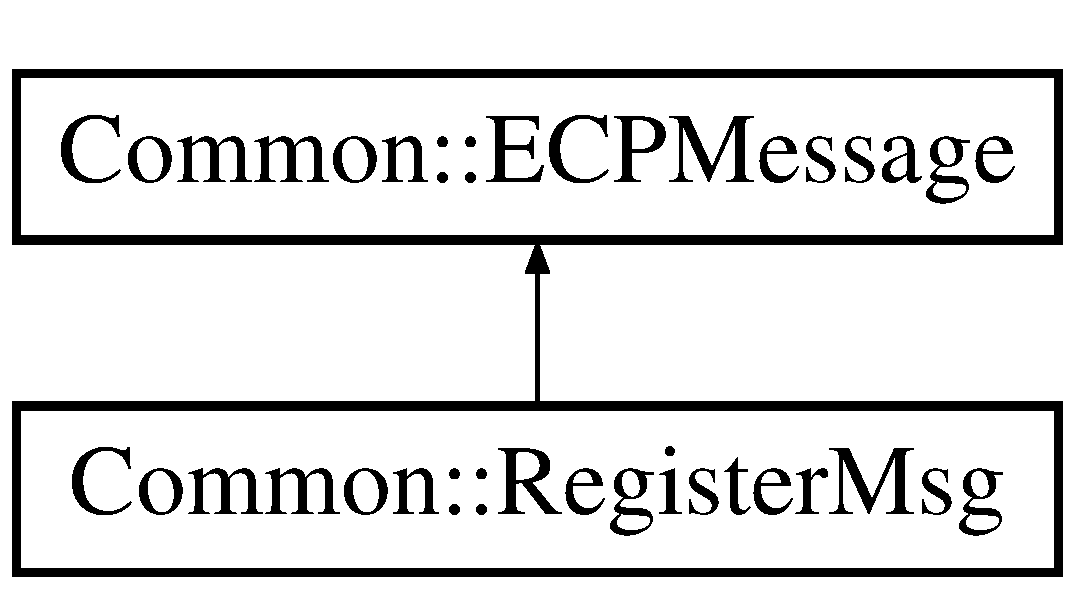
\includegraphics[height=2.000000cm]{class_common_1_1_register_msg}
\end{center}
\end{figure}
\subsection*{Public Member Functions}
\begin{DoxyCompactItemize}
\item 
\hyperlink{class_common_1_1_register_msg_ab97869aa4d99b10fad4df118f91784eb}{Register\-Msg} (int pid=0, int mpi\-Rank=0, std\-::string host=std\-::string(), std\-::string task\-Name=std\-::string(), int A\-Cport=0)
\begin{DoxyCompactList}\small\item\em Constructor. \end{DoxyCompactList}\item 
\hypertarget{class_common_1_1_register_msg_a307245b2ff871bf0e4d8167b3773eaff}{E\-C\-P\-Msg\-Type \hyperlink{class_common_1_1_register_msg_a307245b2ff871bf0e4d8167b3773eaff}{Get\-Type} () const }\label{class_common_1_1_register_msg_a307245b2ff871bf0e4d8167b3773eaff}

\begin{DoxyCompactList}\small\item\em Returns the type of event. \end{DoxyCompactList}\item 
\hypertarget{class_common_1_1_register_msg_a21510f554bed14f14c600da80d6cc030}{int \hyperlink{class_common_1_1_register_msg_a21510f554bed14f14c600da80d6cc030}{Get\-Pid} () const }\label{class_common_1_1_register_msg_a21510f554bed14f14c600da80d6cc030}

\begin{DoxyCompactList}\small\item\em Returns Id of the process where the library will be loaded. \end{DoxyCompactList}\item 
\hypertarget{class_common_1_1_register_msg_a931519d8c96b3af0408b274f23ec7d01}{int \hyperlink{class_common_1_1_register_msg_a931519d8c96b3af0408b274f23ec7d01}{Get\-Mpi\-Rank} () const }\label{class_common_1_1_register_msg_a931519d8c96b3af0408b274f23ec7d01}

\begin{DoxyCompactList}\small\item\em Returns mpi rank. \end{DoxyCompactList}\item 
\hypertarget{class_common_1_1_register_msg_a6a84fcf95b5e4a616fbe52b6c807bf68}{string const \& \hyperlink{class_common_1_1_register_msg_a6a84fcf95b5e4a616fbe52b6c807bf68}{Get\-Host} () const }\label{class_common_1_1_register_msg_a6a84fcf95b5e4a616fbe52b6c807bf68}

\begin{DoxyCompactList}\small\item\em Returns host name where the process is located. \end{DoxyCompactList}\item 
\hypertarget{class_common_1_1_register_msg_afc8d9e7d64970c83c45f0850f3b6f652}{string const \& \hyperlink{class_common_1_1_register_msg_afc8d9e7d64970c83c45f0850f3b6f652}{Get\-Task\-Name} () const }\label{class_common_1_1_register_msg_afc8d9e7d64970c83c45f0850f3b6f652}

\begin{DoxyCompactList}\small\item\em Returns task name. \end{DoxyCompactList}\item 
\hypertarget{class_common_1_1_register_msg_a4bfb4d83fbb9020e9599ab394a57f7b1}{void \hyperlink{class_common_1_1_register_msg_a4bfb4d83fbb9020e9599ab394a57f7b1}{Serialize} (\hyperlink{class_common_1_1_serializer}{Serializer} \&out) const }\label{class_common_1_1_register_msg_a4bfb4d83fbb9020e9599ab394a57f7b1}

\begin{DoxyCompactList}\small\item\em Sends the message. \end{DoxyCompactList}\item 
\hypertarget{class_common_1_1_register_msg_a0a6042f2b893a915c5f2eaf5e6933a6e}{void \hyperlink{class_common_1_1_register_msg_a0a6042f2b893a915c5f2eaf5e6933a6e}{De\-Serialize} (\hyperlink{class_common_1_1_de_serializer}{De\-Serializer} \&in)}\label{class_common_1_1_register_msg_a0a6042f2b893a915c5f2eaf5e6933a6e}

\begin{DoxyCompactList}\small\item\em Receives the message. \end{DoxyCompactList}\end{DoxyCompactItemize}
\subsection*{Additional Inherited Members}


\subsection{Detailed Description}
Represents message that is sent when D\-M\-Lib is registered with analyzer to send event messages. 

\begin{DoxyVersion}{Version}
1.\-0b 
\end{DoxyVersion}
\begin{DoxySince}{Since}
1.\-0b 
\end{DoxySince}
\begin{DoxyAuthor}{Author}
Ania Sikora, 2002 
\end{DoxyAuthor}


\subsection{Constructor \& Destructor Documentation}
\hypertarget{class_common_1_1_register_msg_ab97869aa4d99b10fad4df118f91784eb}{\index{Common\-::\-Register\-Msg@{Common\-::\-Register\-Msg}!Register\-Msg@{Register\-Msg}}
\index{Register\-Msg@{Register\-Msg}!Common::RegisterMsg@{Common\-::\-Register\-Msg}}
\subsubsection[{Register\-Msg}]{\setlength{\rightskip}{0pt plus 5cm}Common\-::\-Register\-Msg\-::\-Register\-Msg (
\begin{DoxyParamCaption}
\item[{int}]{pid = {\ttfamily 0}, }
\item[{int}]{mpi\-Rank = {\ttfamily 0}, }
\item[{std\-::string}]{host = {\ttfamily std\-:\-:string()}, }
\item[{std\-::string}]{task\-Name = {\ttfamily std\-:\-:string()}, }
\item[{int}]{A\-Cport = {\ttfamily 0}}
\end{DoxyParamCaption}
)\hspace{0.3cm}{\ttfamily [inline]}}}\label{class_common_1_1_register_msg_ab97869aa4d99b10fad4df118f91784eb}


Constructor. 


\begin{DoxyParams}{Parameters}
{\em pid} & Id of the process where the library will be registered. \\
\hline
{\em mpi\-Rank} & Mpi rank. \\
\hline
{\em host} & Host where the process is located. \\
\hline
{\em task\-Name} & Name of the task. \\
\hline
\end{DoxyParams}


The documentation for this class was generated from the following files\-:\begin{DoxyCompactItemize}
\item 
Common/E\-C\-P\-Msg.\-h\item 
Common/E\-C\-P\-Msg.\-cpp\end{DoxyCompactItemize}

\hypertarget{class_common_1_1_remote_process}{\section{Common\-:\-:Remote\-Process Class Reference}
\label{class_common_1_1_remote_process}\index{Common\-::\-Remote\-Process@{Common\-::\-Remote\-Process}}
}


Remotely executes a command in another machine.  




{\ttfamily \#include $<$Process.\-h$>$}

Inheritance diagram for Common\-:\-:Remote\-Process\-:\begin{figure}[H]
\begin{center}
\leavevmode
\includegraphics[height=3.000000cm]{class_common_1_1_remote_process}
\end{center}
\end{figure}
\subsection*{Public Member Functions}
\begin{DoxyCompactItemize}
\item 
\hyperlink{class_common_1_1_remote_process_a4391c49d837b2b1c9f5514d09cc82f61}{Remote\-Process} (std\-::string host\-Name, std\-::string command, std\-::string rsh\-Path=std\-::string(\char`\"{}/usr/bin/rsh\char`\"{}))
\begin{DoxyCompactList}\small\item\em Constructor. \end{DoxyCompactList}\item 
\hyperlink{class_common_1_1_remote_process_afcbb01195482dc86fe8294c53ac4d422}{Remote\-Process} (std\-::string host\-Name, std\-::string user\-Name, std\-::string command, std\-::string rsh\-Path=std\-::string(\char`\"{}/usr/bin/rsh\char`\"{}))
\begin{DoxyCompactList}\small\item\em Constructor. \end{DoxyCompactList}\item 
\hypertarget{class_common_1_1_remote_process_a513136e2e9b13380a045f5d78a014afb}{void \hyperlink{class_common_1_1_remote_process_a513136e2e9b13380a045f5d78a014afb}{Set\-Output\-To\-Null} ()}\label{class_common_1_1_remote_process_a513136e2e9b13380a045f5d78a014afb}

\begin{DoxyCompactList}\small\item\em Enables output to null property. \end{DoxyCompactList}\end{DoxyCompactItemize}
\subsection*{Protected Member Functions}
\begin{DoxyCompactItemize}
\item 
\hypertarget{class_common_1_1_remote_process_a8cdc86c2191a88ef97a2a743b484fac5}{int \hyperlink{class_common_1_1_remote_process_a8cdc86c2191a88ef97a2a743b484fac5}{Run} ()}\label{class_common_1_1_remote_process_a8cdc86c2191a88ef97a2a743b484fac5}

\begin{DoxyCompactList}\small\item\em Executes de process. \end{DoxyCompactList}\item 
\hypertarget{class_common_1_1_remote_process_a8542d9bcd4bb05453c046c1497748b18}{std\-::string {\bfseries Get\-Host\-Name} () const }\label{class_common_1_1_remote_process_a8542d9bcd4bb05453c046c1497748b18}

\end{DoxyCompactItemize}
\subsection*{Additional Inherited Members}


\subsection{Detailed Description}
Remotely executes a command in another machine. 

Uses the rsh program to perform the execution of the process.

\begin{DoxyVersion}{Version}
1.\-0b 
\end{DoxyVersion}
\begin{DoxySince}{Since}
1.\-0b 
\end{DoxySince}
\begin{DoxyAuthor}{Author}
Ania Sikora, 2001 
\end{DoxyAuthor}


\subsection{Constructor \& Destructor Documentation}
\hypertarget{class_common_1_1_remote_process_a4391c49d837b2b1c9f5514d09cc82f61}{\index{Common\-::\-Remote\-Process@{Common\-::\-Remote\-Process}!Remote\-Process@{Remote\-Process}}
\index{Remote\-Process@{Remote\-Process}!Common::RemoteProcess@{Common\-::\-Remote\-Process}}
\subsubsection[{Remote\-Process}]{\setlength{\rightskip}{0pt plus 5cm}Common\-::\-Remote\-Process\-::\-Remote\-Process (
\begin{DoxyParamCaption}
\item[{std\-::string}]{host\-Name, }
\item[{std\-::string}]{command, }
\item[{std\-::string}]{rsh\-Path = {\ttfamily std\-:\-:string(\char`\"{}/usr/bin/rsh\char`\"{})}}
\end{DoxyParamCaption}
)\hspace{0.3cm}{\ttfamily [inline]}}}\label{class_common_1_1_remote_process_a4391c49d837b2b1c9f5514d09cc82f61}


Constructor. 


\begin{DoxyParams}{Parameters}
{\em host\-Name} & Host where the command will be executed remotely. \\
\hline
{\em command} & Command to execute. \\
\hline
{\em rsh\-Path} & Local path of the rsh program, default = \char`\"{}/usr/bin/rsh\char`\"{}. \\
\hline
\end{DoxyParams}
\hypertarget{class_common_1_1_remote_process_afcbb01195482dc86fe8294c53ac4d422}{\index{Common\-::\-Remote\-Process@{Common\-::\-Remote\-Process}!Remote\-Process@{Remote\-Process}}
\index{Remote\-Process@{Remote\-Process}!Common::RemoteProcess@{Common\-::\-Remote\-Process}}
\subsubsection[{Remote\-Process}]{\setlength{\rightskip}{0pt plus 5cm}Common\-::\-Remote\-Process\-::\-Remote\-Process (
\begin{DoxyParamCaption}
\item[{std\-::string}]{host\-Name, }
\item[{std\-::string}]{user\-Name, }
\item[{std\-::string}]{command, }
\item[{std\-::string}]{rsh\-Path = {\ttfamily std\-:\-:string(\char`\"{}/usr/bin/rsh\char`\"{})}}
\end{DoxyParamCaption}
)\hspace{0.3cm}{\ttfamily [inline]}}}\label{class_common_1_1_remote_process_afcbb01195482dc86fe8294c53ac4d422}


Constructor. 


\begin{DoxyParams}{Parameters}
{\em host\-Name} & Host where the command will be executed remotely. \\
\hline
{\em command} & Command to execute. \\
\hline
{\em user\-Name} & Name of the user on the host to execute the command. \\
\hline
{\em rsh\-Path} & Local path of the rsh program, default = \char`\"{}/usr/bin/rsh\char`\"{}. \\
\hline
\end{DoxyParams}


The documentation for this class was generated from the following files\-:\begin{DoxyCompactItemize}
\item 
Common/Process.\-h\item 
Common/Process.\-cpp\end{DoxyCompactItemize}

\hypertarget{class_common_1_1_remove_function_call_request}{\section{Common\-:\-:Remove\-Function\-Call\-Request Class Reference}
\label{class_common_1_1_remove_function_call_request}\index{Common\-::\-Remove\-Function\-Call\-Request@{Common\-::\-Remove\-Function\-Call\-Request}}
}


Encapsulates a tuning request to remove all calls to a given function from the given caller function.  




{\ttfamily \#include $<$P\-T\-P\-Msg.\-h$>$}

Inheritance diagram for Common\-:\-:Remove\-Function\-Call\-Request\-:\begin{figure}[H]
\begin{center}
\leavevmode
\includegraphics[height=4.000000cm]{class_common_1_1_remove_function_call_request}
\end{center}
\end{figure}
\subsection*{Public Member Functions}
\begin{DoxyCompactItemize}
\item 
\hyperlink{class_common_1_1_remove_function_call_request_a91cadad0b3bce1f6d0c8212cd079825d}{Remove\-Function\-Call\-Request} (int pid=0, std\-::string const \&func\-Name=std\-::string(), std\-::string const \&caller\-Func=string(), \hyperlink{class_common_1_1_breakpoint}{Breakpoint} const $\ast$brkpt=0)
\begin{DoxyCompactList}\small\item\em Constructor. \end{DoxyCompactList}\item 
\hypertarget{class_common_1_1_remove_function_call_request_ad1ddf3ea5c23b28725463a9a8f33a619}{P\-T\-P\-Msg\-Type \hyperlink{class_common_1_1_remove_function_call_request_ad1ddf3ea5c23b28725463a9a8f33a619}{Get\-Type} () const }\label{class_common_1_1_remove_function_call_request_ad1ddf3ea5c23b28725463a9a8f33a619}

\begin{DoxyCompactList}\small\item\em Returns type of message (P\-T\-P\-Remove\-Func\-Call). \end{DoxyCompactList}\item 
\hypertarget{class_common_1_1_remove_function_call_request_a09ced083b7c54f9ab3278111ec04f2bc}{std\-::string const \& \hyperlink{class_common_1_1_remove_function_call_request_a09ced083b7c54f9ab3278111ec04f2bc}{Get\-Func\-Name} () const }\label{class_common_1_1_remove_function_call_request_a09ced083b7c54f9ab3278111ec04f2bc}

\begin{DoxyCompactList}\small\item\em Returns name of the function to be added. \end{DoxyCompactList}\item 
\hypertarget{class_common_1_1_remove_function_call_request_ade550fe8f74c1bb3dd701dae551d9b16}{std\-::string const \& \hyperlink{class_common_1_1_remove_function_call_request_ade550fe8f74c1bb3dd701dae551d9b16}{Get\-Caller\-Func} () const }\label{class_common_1_1_remove_function_call_request_ade550fe8f74c1bb3dd701dae551d9b16}

\begin{DoxyCompactList}\small\item\em Returns the function caller name. \end{DoxyCompactList}\item 
\hypertarget{class_common_1_1_remove_function_call_request_a7a7d5980c190cd8e2f830352d4eb2f9d}{void \hyperlink{class_common_1_1_remove_function_call_request_a7a7d5980c190cd8e2f830352d4eb2f9d}{Serialize} (\hyperlink{class_common_1_1_serializer}{Serializer} \&out) const }\label{class_common_1_1_remove_function_call_request_a7a7d5980c190cd8e2f830352d4eb2f9d}

\begin{DoxyCompactList}\small\item\em Sends the message. \end{DoxyCompactList}\item 
\hypertarget{class_common_1_1_remove_function_call_request_ac8a636e5865294f6dedd6e340e3a3a7b}{void \hyperlink{class_common_1_1_remove_function_call_request_ac8a636e5865294f6dedd6e340e3a3a7b}{De\-Serialize} (\hyperlink{class_common_1_1_de_serializer}{De\-Serializer} \&in)}\label{class_common_1_1_remove_function_call_request_ac8a636e5865294f6dedd6e340e3a3a7b}

\begin{DoxyCompactList}\small\item\em Receives the message. \end{DoxyCompactList}\end{DoxyCompactItemize}
\subsection*{Additional Inherited Members}


\subsection{Detailed Description}
Encapsulates a tuning request to remove all calls to a given function from the given caller function. 

\begin{DoxyVersion}{Version}
1.\-0 
\end{DoxyVersion}
\begin{DoxySince}{Since}
1.\-0 
\end{DoxySince}
\begin{DoxyAuthor}{Author}
Ania Sikora, 2003 
\end{DoxyAuthor}


\subsection{Constructor \& Destructor Documentation}
\hypertarget{class_common_1_1_remove_function_call_request_a91cadad0b3bce1f6d0c8212cd079825d}{\index{Common\-::\-Remove\-Function\-Call\-Request@{Common\-::\-Remove\-Function\-Call\-Request}!Remove\-Function\-Call\-Request@{Remove\-Function\-Call\-Request}}
\index{Remove\-Function\-Call\-Request@{Remove\-Function\-Call\-Request}!Common::RemoveFunctionCallRequest@{Common\-::\-Remove\-Function\-Call\-Request}}
\subsubsection[{Remove\-Function\-Call\-Request}]{\setlength{\rightskip}{0pt plus 5cm}Common\-::\-Remove\-Function\-Call\-Request\-::\-Remove\-Function\-Call\-Request (
\begin{DoxyParamCaption}
\item[{int}]{pid = {\ttfamily 0}, }
\item[{std\-::string const \&}]{func\-Name = {\ttfamily std\-:\-:string()}, }
\item[{std\-::string const \&}]{caller\-Func = {\ttfamily string()}, }
\item[{{\bf Breakpoint} const $\ast$}]{brkpt = {\ttfamily 0}}
\end{DoxyParamCaption}
)\hspace{0.3cm}{\ttfamily [inline]}}}\label{class_common_1_1_remove_function_call_request_a91cadad0b3bce1f6d0c8212cd079825d}


Constructor. 


\begin{DoxyParams}{Parameters}
{\em pid} & Id of the process where the call will be removed, default 0. \\
\hline
{\em func\-Name} & Name of the function to remove, default \char`\"{}\char`\"{}. \\
\hline
{\em caller\-Func} & Name of the caller function, default \char`\"{}\char`\"{}. \\
\hline
{\em brkpt} & Used for synchronization purposes, the actual tuning will be executed when the execution reaches the breakpoint, default 0. \\
\hline
\end{DoxyParams}


The documentation for this class was generated from the following files\-:\begin{DoxyCompactItemize}
\item 
Common/P\-T\-P\-Msg.\-h\item 
Common/P\-T\-P\-Msg.\-cpp\end{DoxyCompactItemize}

\hypertarget{class_common_1_1_remove_instr_request}{\section{Common\-:\-:Remove\-Instr\-Request Class Reference}
\label{class_common_1_1_remove_instr_request}\index{Common\-::\-Remove\-Instr\-Request@{Common\-::\-Remove\-Instr\-Request}}
}


Represents message sent when analyzer requests to remove instrumentation.  




{\ttfamily \#include $<$P\-T\-P\-Msg.\-h$>$}

Inheritance diagram for Common\-:\-:Remove\-Instr\-Request\-:\begin{figure}[H]
\begin{center}
\leavevmode
\includegraphics[height=3.000000cm]{class_common_1_1_remove_instr_request}
\end{center}
\end{figure}
\subsection*{Public Member Functions}
\begin{DoxyCompactItemize}
\item 
\hyperlink{class_common_1_1_remove_instr_request_ad11aa72688176348501ac84364fb4784}{Remove\-Instr\-Request} (int pid=0, int event\-Id=0, Instr\-Place place=ip\-Func\-Entry)
\begin{DoxyCompactList}\small\item\em Constructor. \end{DoxyCompactList}\item 
\hypertarget{class_common_1_1_remove_instr_request_a23c844af4a248eae68aac682df45fe0e}{P\-T\-P\-Msg\-Type \hyperlink{class_common_1_1_remove_instr_request_a23c844af4a248eae68aac682df45fe0e}{Get\-Type} () const }\label{class_common_1_1_remove_instr_request_a23c844af4a248eae68aac682df45fe0e}

\begin{DoxyCompactList}\small\item\em Returns type of message (P\-T\-P\-Remove\-Instr). \end{DoxyCompactList}\item 
\hypertarget{class_common_1_1_remove_instr_request_a8bd7683fc30ee5f5fb531c2422e6a535}{int \hyperlink{class_common_1_1_remove_instr_request_a8bd7683fc30ee5f5fb531c2422e6a535}{Get\-Pid} () const }\label{class_common_1_1_remove_instr_request_a8bd7683fc30ee5f5fb531c2422e6a535}

\begin{DoxyCompactList}\small\item\em Returns the process id. \end{DoxyCompactList}\item 
\hypertarget{class_common_1_1_remove_instr_request_a53090f42338ccb963d38799b0cc4ef4b}{int \hyperlink{class_common_1_1_remove_instr_request_a53090f42338ccb963d38799b0cc4ef4b}{Get\-Event\-Id} () const }\label{class_common_1_1_remove_instr_request_a53090f42338ccb963d38799b0cc4ef4b}

\begin{DoxyCompactList}\small\item\em Returns the event id. \end{DoxyCompactList}\item 
\hypertarget{class_common_1_1_remove_instr_request_af6bd2c0ffb341be5427e04de01140a8c}{Instr\-Place \hyperlink{class_common_1_1_remove_instr_request_af6bd2c0ffb341be5427e04de01140a8c}{Get\-Instr\-Place} () const }\label{class_common_1_1_remove_instr_request_af6bd2c0ffb341be5427e04de01140a8c}

\begin{DoxyCompactList}\small\item\em Returns the place where the instruction should be removed. \end{DoxyCompactList}\item 
\hypertarget{class_common_1_1_remove_instr_request_ac8c54f924e923d990eec86f6fe3d0594}{void \hyperlink{class_common_1_1_remove_instr_request_ac8c54f924e923d990eec86f6fe3d0594}{Serialize} (\hyperlink{class_common_1_1_serializer}{Serializer} \&out) const }\label{class_common_1_1_remove_instr_request_ac8c54f924e923d990eec86f6fe3d0594}

\begin{DoxyCompactList}\small\item\em Sends the message. \end{DoxyCompactList}\item 
\hypertarget{class_common_1_1_remove_instr_request_a0d4fd00d0e6a4579e5b180c07959d239}{void \hyperlink{class_common_1_1_remove_instr_request_a0d4fd00d0e6a4579e5b180c07959d239}{De\-Serialize} (\hyperlink{class_common_1_1_de_serializer}{De\-Serializer} \&in)}\label{class_common_1_1_remove_instr_request_a0d4fd00d0e6a4579e5b180c07959d239}

\begin{DoxyCompactList}\small\item\em Receives the message. \end{DoxyCompactList}\end{DoxyCompactItemize}


\subsection{Detailed Description}
Represents message sent when analyzer requests to remove instrumentation. 

\begin{DoxyVersion}{Version}
1.\-0b 
\end{DoxyVersion}
\begin{DoxySince}{Since}
1.\-0b 
\end{DoxySince}
\begin{DoxyAuthor}{Author}
Ania Sikora, 2003 
\end{DoxyAuthor}


\subsection{Constructor \& Destructor Documentation}
\hypertarget{class_common_1_1_remove_instr_request_ad11aa72688176348501ac84364fb4784}{\index{Common\-::\-Remove\-Instr\-Request@{Common\-::\-Remove\-Instr\-Request}!Remove\-Instr\-Request@{Remove\-Instr\-Request}}
\index{Remove\-Instr\-Request@{Remove\-Instr\-Request}!Common::RemoveInstrRequest@{Common\-::\-Remove\-Instr\-Request}}
\subsubsection[{Remove\-Instr\-Request}]{\setlength{\rightskip}{0pt plus 5cm}Common\-::\-Remove\-Instr\-Request\-::\-Remove\-Instr\-Request (
\begin{DoxyParamCaption}
\item[{int}]{pid = {\ttfamily 0}, }
\item[{int}]{event\-Id = {\ttfamily 0}, }
\item[{Instr\-Place}]{place = {\ttfamily ipFuncEntry}}
\end{DoxyParamCaption}
)\hspace{0.3cm}{\ttfamily [inline]}}}\label{class_common_1_1_remove_instr_request_ad11aa72688176348501ac84364fb4784}


Constructor. 


\begin{DoxyParams}{Parameters}
{\em pid} & Id of the process where the instrumentation will be removed, default 0. \\
\hline
{\em event\-Id} & \hyperlink{class_common_1_1_event}{Event} id, default 0. \\
\hline
{\em place} & Place where the instrumentation will be removed, default ip\-Func\-Entry. \\
\hline
\end{DoxyParams}


The documentation for this class was generated from the following files\-:\begin{DoxyCompactItemize}
\item 
Common/P\-T\-P\-Msg.\-h\item 
Common/P\-T\-P\-Msg.\-cpp\end{DoxyCompactItemize}

\hypertarget{class_common_1_1_replace_function_request}{\section{Common\-:\-:Replace\-Function\-Request Class Reference}
\label{class_common_1_1_replace_function_request}\index{Common\-::\-Replace\-Function\-Request@{Common\-::\-Replace\-Function\-Request}}
}


Encapsulates a tuning request to replace all calls to a function inside a process with calls to another function.  




{\ttfamily \#include $<$P\-T\-P\-Msg.\-h$>$}

Inheritance diagram for Common\-:\-:Replace\-Function\-Request\-:\begin{figure}[H]
\begin{center}
\leavevmode
\includegraphics[height=4.000000cm]{class_common_1_1_replace_function_request}
\end{center}
\end{figure}
\subsection*{Public Member Functions}
\begin{DoxyCompactItemize}
\item 
\hyperlink{class_common_1_1_replace_function_request_a10fc14a5a61d9497d972a2ec57b02ebe}{Replace\-Function\-Request} (int pid=0, std\-::string const \&old\-Func=std\-::string(), std\-::string const \&new\-Func=std\-::string(), \hyperlink{class_common_1_1_breakpoint}{Breakpoint} $\ast$brkpt=0)
\begin{DoxyCompactList}\small\item\em Constructor. \end{DoxyCompactList}\item 
\hypertarget{class_common_1_1_replace_function_request_a7bb3f7efba25a1566efe4ccc3054cd63}{P\-T\-P\-Msg\-Type \hyperlink{class_common_1_1_replace_function_request_a7bb3f7efba25a1566efe4ccc3054cd63}{Get\-Type} () const }\label{class_common_1_1_replace_function_request_a7bb3f7efba25a1566efe4ccc3054cd63}

\begin{DoxyCompactList}\small\item\em Returns type of message (P\-T\-P\-Replace\-Function). \end{DoxyCompactList}\item 
\hypertarget{class_common_1_1_replace_function_request_a86dc0fe0546f0b4d331116f68f8c45f0}{std\-::string const \& \hyperlink{class_common_1_1_replace_function_request_a86dc0fe0546f0b4d331116f68f8c45f0}{Get\-Old\-Function} () const }\label{class_common_1_1_replace_function_request_a86dc0fe0546f0b4d331116f68f8c45f0}

\begin{DoxyCompactList}\small\item\em Returns a string containing the name of the function to replace. \end{DoxyCompactList}\item 
\hypertarget{class_common_1_1_replace_function_request_a0285b26773d41dc9b2b6289ce104102c}{std\-::string const \& \hyperlink{class_common_1_1_replace_function_request_a0285b26773d41dc9b2b6289ce104102c}{Get\-New\-Function} () const }\label{class_common_1_1_replace_function_request_a0285b26773d41dc9b2b6289ce104102c}

\begin{DoxyCompactList}\small\item\em Returns a string containing the name of the function added. \end{DoxyCompactList}\item 
\hypertarget{class_common_1_1_replace_function_request_a1ba53378e26e28ff1052285492c50fd4}{void \hyperlink{class_common_1_1_replace_function_request_a1ba53378e26e28ff1052285492c50fd4}{Serialize} (\hyperlink{class_common_1_1_serializer}{Serializer} \&out) const }\label{class_common_1_1_replace_function_request_a1ba53378e26e28ff1052285492c50fd4}

\begin{DoxyCompactList}\small\item\em Sends the message. \end{DoxyCompactList}\item 
\hypertarget{class_common_1_1_replace_function_request_ad000a60b1e0bc5c06ec40fd15e8f7080}{void \hyperlink{class_common_1_1_replace_function_request_ad000a60b1e0bc5c06ec40fd15e8f7080}{De\-Serialize} (\hyperlink{class_common_1_1_de_serializer}{De\-Serializer} \&in)}\label{class_common_1_1_replace_function_request_ad000a60b1e0bc5c06ec40fd15e8f7080}

\begin{DoxyCompactList}\small\item\em Receives the message. \end{DoxyCompactList}\end{DoxyCompactItemize}
\subsection*{Additional Inherited Members}


\subsection{Detailed Description}
Encapsulates a tuning request to replace all calls to a function inside a process with calls to another function. 

\begin{DoxyVersion}{Version}
1.\-0b 
\end{DoxyVersion}
\begin{DoxySince}{Since}
1.\-0b 
\end{DoxySince}
\begin{DoxyAuthor}{Author}
Ania Sikora, 2003 
\end{DoxyAuthor}


\subsection{Constructor \& Destructor Documentation}
\hypertarget{class_common_1_1_replace_function_request_a10fc14a5a61d9497d972a2ec57b02ebe}{\index{Common\-::\-Replace\-Function\-Request@{Common\-::\-Replace\-Function\-Request}!Replace\-Function\-Request@{Replace\-Function\-Request}}
\index{Replace\-Function\-Request@{Replace\-Function\-Request}!Common::ReplaceFunctionRequest@{Common\-::\-Replace\-Function\-Request}}
\subsubsection[{Replace\-Function\-Request}]{\setlength{\rightskip}{0pt plus 5cm}Common\-::\-Replace\-Function\-Request\-::\-Replace\-Function\-Request (
\begin{DoxyParamCaption}
\item[{int}]{pid = {\ttfamily 0}, }
\item[{std\-::string const \&}]{old\-Func = {\ttfamily std\-:\-:string()}, }
\item[{std\-::string const \&}]{new\-Func = {\ttfamily std\-:\-:string()}, }
\item[{{\bf Breakpoint} $\ast$}]{brkpt = {\ttfamily 0}}
\end{DoxyParamCaption}
)\hspace{0.3cm}{\ttfamily [inline]}}}\label{class_common_1_1_replace_function_request_a10fc14a5a61d9497d972a2ec57b02ebe}


Constructor. 


\begin{DoxyParams}{Parameters}
{\em pid} & Id of the process where the function will be replaced, default 0. \\
\hline
{\em old\-Func} & Name of the function to replace, default \char`\"{}\char`\"{}. \\
\hline
{\em new\-Func} & Name of the function to add, default \char`\"{}\char`\"{}. \\
\hline
{\em brkpt} & Used for synchronization purposes, the actual tuning will be executed when the execution reaches the breakpoint, default 0. \\
\hline
\end{DoxyParams}


The documentation for this class was generated from the following files\-:\begin{DoxyCompactItemize}
\item 
Common/P\-T\-P\-Msg.\-h\item 
Common/P\-T\-P\-Msg.\-cpp\end{DoxyCompactItemize}

\hypertarget{class_common_1_1_semaphore}{\section{Common\-:\-:Semaphore Class Reference}
\label{class_common_1_1_semaphore}\index{Common\-::\-Semaphore@{Common\-::\-Semaphore}}
}


Synchronizes access to a resource.  




{\ttfamily \#include $<$sync.\-h$>$}

\subsection*{Public Member Functions}
\begin{DoxyCompactItemize}
\item 
\hyperlink{class_common_1_1_semaphore_af69fece31d41c390cb08d9c4abe0a67f}{Semaphore} (int initial\-Value=0, bool cross\-Process=false)
\begin{DoxyCompactList}\small\item\em Constructor. \end{DoxyCompactList}\item 
\hypertarget{class_common_1_1_semaphore_a4c9eebd8d0a6308f88da72faff8d7185}{\hyperlink{class_common_1_1_semaphore_a4c9eebd8d0a6308f88da72faff8d7185}{$\sim$\-Semaphore} ()}\label{class_common_1_1_semaphore_a4c9eebd8d0a6308f88da72faff8d7185}

\begin{DoxyCompactList}\small\item\em Destructor. \end{DoxyCompactList}\item 
void \hyperlink{class_common_1_1_semaphore_a72aabebf026e3a8b1f3e4d0fa8ee1eda}{Wait} ()
\begin{DoxyCompactList}\small\item\em Stops the current thread until the access to the resource is open. \end{DoxyCompactList}\item 
bool \hyperlink{class_common_1_1_semaphore_a2965d5aaefb8b178c525a6e9df36dd60}{Try\-Wait} ()
\begin{DoxyCompactList}\small\item\em Returns true if the access to the resource is open, false otherwise. \end{DoxyCompactList}\item 
void \hyperlink{class_common_1_1_semaphore_a1992c8b46527c96756ba6d9a1c754715}{Post} ()
\begin{DoxyCompactList}\small\item\em Gives a signal to the semaphore indicating that a client has stopped using the resource. \end{DoxyCompactList}\end{DoxyCompactItemize}
\subsection*{Protected Member Functions}
\begin{DoxyCompactItemize}
\item 
\hypertarget{class_common_1_1_semaphore_a718f317dc5f0a37c0f164cbaf29982d4}{{\bfseries Semaphore} (sem\-\_\-t s)}\label{class_common_1_1_semaphore_a718f317dc5f0a37c0f164cbaf29982d4}

\end{DoxyCompactItemize}
\subsection*{Protected Attributes}
\begin{DoxyCompactItemize}
\item 
\hypertarget{class_common_1_1_semaphore_a34fd832be9882679d1f0e2bb256613b5}{sem\-\_\-t {\bfseries \-\_\-semaphore}}\label{class_common_1_1_semaphore_a34fd832be9882679d1f0e2bb256613b5}

\end{DoxyCompactItemize}


\subsection{Detailed Description}
Synchronizes access to a resource. 

A semaphore is generally used as a synchronization object between multiple threads or to protect a limited and finite resource such as a memory or thread pool. The semaphore has a counter which only permits access by one or more threads when the value of the semaphore is non-\/zero. Each access reduces the current value of the semaphore by 1. One or more threads can wait on a semaphore until it is no longer 0, and hence the semaphore can be used as a simple thread synchronization object to enable one thread to pause others until the thread is ready or has provided data for them.

\begin{DoxyVersion}{Version}
1.\-0b 
\end{DoxyVersion}
\begin{DoxySince}{Since}
1.\-0b 
\end{DoxySince}
\begin{DoxyAuthor}{Author}
Ania Sikora, 2002 
\end{DoxyAuthor}


\subsection{Constructor \& Destructor Documentation}
\hypertarget{class_common_1_1_semaphore_af69fece31d41c390cb08d9c4abe0a67f}{\index{Common\-::\-Semaphore@{Common\-::\-Semaphore}!Semaphore@{Semaphore}}
\index{Semaphore@{Semaphore}!Common::Semaphore@{Common\-::\-Semaphore}}
\subsubsection[{Semaphore}]{\setlength{\rightskip}{0pt plus 5cm}Common\-::\-Semaphore\-::\-Semaphore (
\begin{DoxyParamCaption}
\item[{int}]{initial\-Value = {\ttfamily 0}, }
\item[{bool}]{cross\-Process = {\ttfamily false}}
\end{DoxyParamCaption}
)\hspace{0.3cm}{\ttfamily [inline]}}}\label{class_common_1_1_semaphore_af69fece31d41c390cb08d9c4abe0a67f}


Constructor. 


\begin{DoxyParams}{Parameters}
{\em initial\-Value} & Initial value of the semaphore, default 0. \\
\hline
{\em cross\-Process} & Flag indicating whether or not the semaphore should be shared with forked processes, default false. \\
\hline
\end{DoxyParams}


\subsection{Member Function Documentation}
\hypertarget{class_common_1_1_semaphore_a1992c8b46527c96756ba6d9a1c754715}{\index{Common\-::\-Semaphore@{Common\-::\-Semaphore}!Post@{Post}}
\index{Post@{Post}!Common::Semaphore@{Common\-::\-Semaphore}}
\subsubsection[{Post}]{\setlength{\rightskip}{0pt plus 5cm}void Semaphore\-::\-Post (
\begin{DoxyParamCaption}
{}
\end{DoxyParamCaption}
)}}\label{class_common_1_1_semaphore_a1992c8b46527c96756ba6d9a1c754715}


Gives a signal to the semaphore indicating that a client has stopped using the resource. 

Posting to a semaphore increments its current value and releases the first thread waiting for the semaphore if it is currently at 0. \hypertarget{class_common_1_1_semaphore_a2965d5aaefb8b178c525a6e9df36dd60}{\index{Common\-::\-Semaphore@{Common\-::\-Semaphore}!Try\-Wait@{Try\-Wait}}
\index{Try\-Wait@{Try\-Wait}!Common::Semaphore@{Common\-::\-Semaphore}}
\subsubsection[{Try\-Wait}]{\setlength{\rightskip}{0pt plus 5cm}bool Semaphore\-::\-Try\-Wait (
\begin{DoxyParamCaption}
{}
\end{DoxyParamCaption}
)}}\label{class_common_1_1_semaphore_a2965d5aaefb8b178c525a6e9df36dd60}


Returns true if the access to the resource is open, false otherwise. 

Try\-Wait is a non-\/blocking variant of Wait. If the semaphore counter is greater than 0, then the thread is accepted and the semaphore counter is decreased. If the semaphore counter is 0 Try\-Wait returns immediately with false. \hypertarget{class_common_1_1_semaphore_a72aabebf026e3a8b1f3e4d0fa8ee1eda}{\index{Common\-::\-Semaphore@{Common\-::\-Semaphore}!Wait@{Wait}}
\index{Wait@{Wait}!Common::Semaphore@{Common\-::\-Semaphore}}
\subsubsection[{Wait}]{\setlength{\rightskip}{0pt plus 5cm}void Semaphore\-::\-Wait (
\begin{DoxyParamCaption}
{}
\end{DoxyParamCaption}
)}}\label{class_common_1_1_semaphore_a72aabebf026e3a8b1f3e4d0fa8ee1eda}


Stops the current thread until the access to the resource is open. 

Wait is used to keep a thread held until the semaphore counter is greater than 0. If the current thread is held, then another thread must increment the semaphore. Once the thread is accepted, the semaphore is automatically decremented, and the thread continues execution. 

The documentation for this class was generated from the following files\-:\begin{DoxyCompactItemize}
\item 
Common/sync.\-h\item 
Common/sync.\-cpp\end{DoxyCompactItemize}

\hypertarget{class_common_1_1_serializable}{\section{Common\-:\-:Serializable Class Reference}
\label{class_common_1_1_serializable}\index{Common\-::\-Serializable@{Common\-::\-Serializable}}
}


Abstract class, makes an object able to be passed through a stream using \hyperlink{class_common_1_1_serializer}{Serializer} and \hyperlink{class_common_1_1_de_serializer}{De\-Serializer} objects.  




{\ttfamily \#include $<$Serial.\-h$>$}

Inheritance diagram for Common\-:\-:Serializable\-:\begin{figure}[H]
\begin{center}
\leavevmode
\includegraphics[height=0.906883cm]{class_common_1_1_serializable}
\end{center}
\end{figure}
\subsection*{Public Member Functions}
\begin{DoxyCompactItemize}
\item 
\hypertarget{class_common_1_1_serializable_a09a6076f46669dda73a69adb2417b078}{virtual \hyperlink{class_common_1_1_serializable_a09a6076f46669dda73a69adb2417b078}{$\sim$\-Serializable} ()}\label{class_common_1_1_serializable_a09a6076f46669dda73a69adb2417b078}

\begin{DoxyCompactList}\small\item\em Destructor. \end{DoxyCompactList}\item 
\hypertarget{class_common_1_1_serializable_af75f78fb713d03e9fa9adad209e7d0b6}{virtual void \hyperlink{class_common_1_1_serializable_af75f78fb713d03e9fa9adad209e7d0b6}{Serialize} (\hyperlink{class_common_1_1_serializer}{Serializer} \&out) const =0}\label{class_common_1_1_serializable_af75f78fb713d03e9fa9adad209e7d0b6}

\begin{DoxyCompactList}\small\item\em Sends the message header. \end{DoxyCompactList}\item 
\hypertarget{class_common_1_1_serializable_a90bf86a849f5cda5697ea7434c7a980a}{virtual void \hyperlink{class_common_1_1_serializable_a90bf86a849f5cda5697ea7434c7a980a}{De\-Serialize} (\hyperlink{class_common_1_1_de_serializer}{De\-Serializer} \&in)=0}\label{class_common_1_1_serializable_a90bf86a849f5cda5697ea7434c7a980a}

\begin{DoxyCompactList}\small\item\em Receives the message header. \end{DoxyCompactList}\end{DoxyCompactItemize}


\subsection{Detailed Description}
Abstract class, makes an object able to be passed through a stream using \hyperlink{class_common_1_1_serializer}{Serializer} and \hyperlink{class_common_1_1_de_serializer}{De\-Serializer} objects. 

\begin{DoxyVersion}{Version}
1.\-0b 
\end{DoxyVersion}
\begin{DoxySince}{Since}
1.\-0b 
\end{DoxySince}
\begin{DoxyAuthor}{Author}
Ania Sikora, 2002 
\end{DoxyAuthor}


The documentation for this class was generated from the following file\-:\begin{DoxyCompactItemize}
\item 
Common/Serial.\-h\end{DoxyCompactItemize}

\hypertarget{class_common_1_1_serializer}{\section{Common\-:\-:Serializer Class Reference}
\label{class_common_1_1_serializer}\index{Common\-::\-Serializer@{Common\-::\-Serializer}}
}


Abstract class, prepares objects to be passed on a stream.  




{\ttfamily \#include $<$Serial.\-h$>$}

Inheritance diagram for Common\-:\-:Serializer\-:\begin{figure}[H]
\begin{center}
\leavevmode
\includegraphics[height=2.000000cm]{class_common_1_1_serializer}
\end{center}
\end{figure}
\subsection*{Public Member Functions}
\begin{DoxyCompactItemize}
\item 
\hypertarget{class_common_1_1_serializer_ab21ce88a2dbb0a62f046d576cefc2981}{virtual void \hyperlink{class_common_1_1_serializer_ab21ce88a2dbb0a62f046d576cefc2981}{Put\-Byte} (byte\-\_\-t b)=0}\label{class_common_1_1_serializer_ab21ce88a2dbb0a62f046d576cefc2981}

\begin{DoxyCompactList}\small\item\em Adds the size of a serialized byte. \end{DoxyCompactList}\item 
\hypertarget{class_common_1_1_serializer_ad5a7ba2087b4e6afd657a35ab7c992c4}{virtual void \hyperlink{class_common_1_1_serializer_ad5a7ba2087b4e6afd657a35ab7c992c4}{Put\-Char} (char\-\_\-t c)=0}\label{class_common_1_1_serializer_ad5a7ba2087b4e6afd657a35ab7c992c4}

\begin{DoxyCompactList}\small\item\em Adds the size of a serialized char. \end{DoxyCompactList}\item 
\hypertarget{class_common_1_1_serializer_a8b2c0544de040591c37c9b0bd9dcfc8f}{virtual void \hyperlink{class_common_1_1_serializer_a8b2c0544de040591c37c9b0bd9dcfc8f}{Put\-Bool} (bool\-\_\-t b)=0}\label{class_common_1_1_serializer_a8b2c0544de040591c37c9b0bd9dcfc8f}

\begin{DoxyCompactList}\small\item\em Adds the size of a serialized bool. \end{DoxyCompactList}\item 
\hypertarget{class_common_1_1_serializer_a7a9eaa08853d2b7634f2fe34f1f74618}{virtual void \hyperlink{class_common_1_1_serializer_a7a9eaa08853d2b7634f2fe34f1f74618}{Put\-Short} (short\-\_\-t s)=0}\label{class_common_1_1_serializer_a7a9eaa08853d2b7634f2fe34f1f74618}

\begin{DoxyCompactList}\small\item\em Adds the size of a serialized short. \end{DoxyCompactList}\item 
\hypertarget{class_common_1_1_serializer_ace5e0ab73827b1e1e22e15494a4b63fc}{virtual void \hyperlink{class_common_1_1_serializer_ace5e0ab73827b1e1e22e15494a4b63fc}{Put\-Int} (int\-\_\-t i)=0}\label{class_common_1_1_serializer_ace5e0ab73827b1e1e22e15494a4b63fc}

\begin{DoxyCompactList}\small\item\em Adds the size of a serialized int. \end{DoxyCompactList}\item 
\hypertarget{class_common_1_1_serializer_a81707bcd851d97120e44738605eb2c61}{virtual void \hyperlink{class_common_1_1_serializer_a81707bcd851d97120e44738605eb2c61}{Put\-Long} (long\-\_\-t l)=0}\label{class_common_1_1_serializer_a81707bcd851d97120e44738605eb2c61}

\begin{DoxyCompactList}\small\item\em Adds the size of a serialized long. \end{DoxyCompactList}\item 
\hypertarget{class_common_1_1_serializer_aae8365d415cefb35dbd5ec871a2c8ea3}{virtual void \hyperlink{class_common_1_1_serializer_aae8365d415cefb35dbd5ec871a2c8ea3}{Put\-Double} (double\-\_\-t d)=0}\label{class_common_1_1_serializer_aae8365d415cefb35dbd5ec871a2c8ea3}

\begin{DoxyCompactList}\small\item\em Adds the size of a serialized double. \end{DoxyCompactList}\item 
\hypertarget{class_common_1_1_serializer_a222ec745d1a6a144e02e196b2b4b273a}{virtual void \hyperlink{class_common_1_1_serializer_a222ec745d1a6a144e02e196b2b4b273a}{Put\-String} (std\-::string const \&str)=0}\label{class_common_1_1_serializer_a222ec745d1a6a144e02e196b2b4b273a}

\begin{DoxyCompactList}\small\item\em Adds the size of a serialized string. \end{DoxyCompactList}\item 
\hypertarget{class_common_1_1_serializer_a53a4cff20c5f3fc5a8c7903aaf31e7ac}{virtual void \hyperlink{class_common_1_1_serializer_a53a4cff20c5f3fc5a8c7903aaf31e7ac}{Put\-Buffer} (char const $\ast$buffer, int buffer\-Size)=0}\label{class_common_1_1_serializer_a53a4cff20c5f3fc5a8c7903aaf31e7ac}

\begin{DoxyCompactList}\small\item\em Adds the size of a serialized buffer. \end{DoxyCompactList}\end{DoxyCompactItemize}


\subsection{Detailed Description}
Abstract class, prepares objects to be passed on a stream. 

\begin{DoxyVersion}{Version}
1.\-0b 
\end{DoxyVersion}
\begin{DoxySince}{Since}
1.\-0b 
\end{DoxySince}
\begin{DoxyAuthor}{Author}
Ania Sikora, 2002 
\end{DoxyAuthor}


The documentation for this class was generated from the following file\-:\begin{DoxyCompactItemize}
\item 
Common/Serial.\-h\end{DoxyCompactItemize}

\hypertarget{class_common_1_1_server_socket}{\section{Common\-:\-:Server\-Socket Class Reference}
\label{class_common_1_1_server_socket}\index{Common\-::\-Server\-Socket@{Common\-::\-Server\-Socket}}
}


Holds a \hyperlink{class_common_1_1_socket_base}{Socket\-Base} object and represents a T\-C\-P/\-I\-P server socket.  




{\ttfamily \#include $<$Socket.\-h$>$}

\subsection*{Public Member Functions}
\begin{DoxyCompactItemize}
\item 
\hyperlink{class_common_1_1_server_socket_a5f4eb8602a8dc21db806b7d45cd9d887}{Server\-Socket} (int port, int back\-Log=5)
\begin{DoxyCompactList}\small\item\em Constructor. \end{DoxyCompactList}\item 
\hypertarget{class_common_1_1_server_socket_a2d330848e8f6eb4858d0a6037c734f1b}{void \hyperlink{class_common_1_1_server_socket_a2d330848e8f6eb4858d0a6037c734f1b}{Listen} ()}\label{class_common_1_1_server_socket_a2d330848e8f6eb4858d0a6037c734f1b}

\begin{DoxyCompactList}\small\item\em Sets the socket to a listening state. \end{DoxyCompactList}\item 
\hypertarget{class_common_1_1_server_socket_a1dd43d8a49feb6b39b26b3616b8d5273}{Socket\-Ptr \hyperlink{class_common_1_1_server_socket_a1dd43d8a49feb6b39b26b3616b8d5273}{Accept} ()}\label{class_common_1_1_server_socket_a1dd43d8a49feb6b39b26b3616b8d5273}

\begin{DoxyCompactList}\small\item\em Accepts a connection and creates a socket. \end{DoxyCompactList}\item 
\hypertarget{class_common_1_1_server_socket_ace551f50347ca514eead71c6775230e3}{Socket\-Ptr \hyperlink{class_common_1_1_server_socket_ace551f50347ca514eead71c6775230e3}{Accept} (int timeout\-Ms)}\label{class_common_1_1_server_socket_ace551f50347ca514eead71c6775230e3}

\begin{DoxyCompactList}\small\item\em Accepts a connection and creates a socket, waits the given timeout. \end{DoxyCompactList}\item 
\hypertarget{class_common_1_1_server_socket_a4385aed2d50f6f4677405063f41b7ff8}{\hyperlink{class_common_1_1_address}{Address} const \& \hyperlink{class_common_1_1_server_socket_a4385aed2d50f6f4677405063f41b7ff8}{Get\-Address} () const }\label{class_common_1_1_server_socket_a4385aed2d50f6f4677405063f41b7ff8}

\begin{DoxyCompactList}\small\item\em Returns local server address. \end{DoxyCompactList}\item 
\hypertarget{class_common_1_1_server_socket_af429415c5735b7b3136fd2112888222d}{int \hyperlink{class_common_1_1_server_socket_af429415c5735b7b3136fd2112888222d}{Get\-Local\-Port} () const }\label{class_common_1_1_server_socket_af429415c5735b7b3136fd2112888222d}

\begin{DoxyCompactList}\small\item\em Returns the port the socket is listening to. \end{DoxyCompactList}\item 
\hypertarget{class_common_1_1_server_socket_a796a2ec7fd019213799a0c1e5e73ef3d}{int \hyperlink{class_common_1_1_server_socket_a796a2ec7fd019213799a0c1e5e73ef3d}{Get\-Handle} () const }\label{class_common_1_1_server_socket_a796a2ec7fd019213799a0c1e5e73ef3d}

\begin{DoxyCompactList}\small\item\em Returns socket handle. \end{DoxyCompactList}\end{DoxyCompactItemize}


\subsection{Detailed Description}
Holds a \hyperlink{class_common_1_1_socket_base}{Socket\-Base} object and represents a T\-C\-P/\-I\-P server socket. 

All the functions on this class are present on the \hyperlink{class_common_1_1_socket_base}{Socket\-Base} class and have the same functionality.

\begin{DoxyVersion}{Version}
1.\-0b 
\end{DoxyVersion}
\begin{DoxySince}{Since}
1.\-0b 
\end{DoxySince}
\begin{DoxyAuthor}{Author}
Ania Sikora, 2002 
\end{DoxyAuthor}


\subsection{Constructor \& Destructor Documentation}
\hypertarget{class_common_1_1_server_socket_a5f4eb8602a8dc21db806b7d45cd9d887}{\index{Common\-::\-Server\-Socket@{Common\-::\-Server\-Socket}!Server\-Socket@{Server\-Socket}}
\index{Server\-Socket@{Server\-Socket}!Common::ServerSocket@{Common\-::\-Server\-Socket}}
\subsubsection[{Server\-Socket}]{\setlength{\rightskip}{0pt plus 5cm}Server\-Socket\-::\-Server\-Socket (
\begin{DoxyParamCaption}
\item[{int}]{port, }
\item[{int}]{back\-Log = {\ttfamily 5}}
\end{DoxyParamCaption}
)}}\label{class_common_1_1_server_socket_a5f4eb8602a8dc21db806b7d45cd9d887}


Constructor. 


\begin{DoxyParams}{Parameters}
{\em back\-Log} & Maximum length of the queue for pending connections.\\
\hline
\end{DoxyParams}

\begin{DoxyExceptions}{Exceptions}
{\em Sys\-Exception.} & \\
\hline
\end{DoxyExceptions}


The documentation for this class was generated from the following files\-:\begin{DoxyCompactItemize}
\item 
Common/Socket.\-h\item 
Common/Socket.\-cpp\end{DoxyCompactItemize}

\hypertarget{class_service}{\section{Service Class Reference}
\label{class_service}\index{Service@{Service}}
}


Provides methods to work with Event\-Collector\-Handlers lists. Holds a list of Event\-Coll\-Handler and a reference to the reactor. Provides methods to add and remove handlers from the list.  




{\ttfamily \#include $<$Service.\-h$>$}

\subsection*{Public Member Functions}
\begin{DoxyCompactItemize}
\item 
\hyperlink{class_service_afdf4b841bca28fe00ee4525e2882ff72}{Service} (\hyperlink{class_common_1_1_reactor}{Reactor} \&reactor)
\begin{DoxyCompactList}\small\item\em Constructor. \end{DoxyCompactList}\item 
\hypertarget{class_service_af6c3577b59652ac817d1d76aaccee904}{\hyperlink{class_service_af6c3577b59652ac817d1d76aaccee904}{$\sim$\-Service} ()}\label{class_service_af6c3577b59652ac817d1d76aaccee904}

\begin{DoxyCompactList}\small\item\em Destructor, deletes the handlers and the references to them. \end{DoxyCompactList}\item 
void \hyperlink{class_service_a7e563ec252f817e5a1cdfb40d07dd8fb}{Add} (\hyperlink{class_e_c_p_handler}{E\-C\-P\-Handler} $\ast$handler)
\begin{DoxyCompactList}\small\item\em Adds a handler to the list and sets its service to this. \end{DoxyCompactList}\item 
void \hyperlink{class_service_a060c72a96167cd02b72287e607b0f21c}{Remove} (\hyperlink{class_e_c_p_handler}{E\-C\-P\-Handler} $\ast$handler)
\begin{DoxyCompactList}\small\item\em Unregisters the handler from the reactor and removes it from the list. \end{DoxyCompactList}\end{DoxyCompactItemize}


\subsection{Detailed Description}
Provides methods to work with Event\-Collector\-Handlers lists. Holds a list of Event\-Coll\-Handler and a reference to the reactor. Provides methods to add and remove handlers from the list. 

\subsection{Constructor \& Destructor Documentation}
\hypertarget{class_service_afdf4b841bca28fe00ee4525e2882ff72}{\index{Service@{Service}!Service@{Service}}
\index{Service@{Service}!Service@{Service}}
\subsubsection[{Service}]{\setlength{\rightskip}{0pt plus 5cm}Service\-::\-Service (
\begin{DoxyParamCaption}
\item[{{\bf Reactor} \&}]{reactor}
\end{DoxyParamCaption}
)\hspace{0.3cm}{\ttfamily [inline]}}}\label{class_service_afdf4b841bca28fe00ee4525e2882ff72}


Constructor. 


\begin{DoxyParams}{Parameters}
{\em reactor} & Reactor of the application \\
\hline
\end{DoxyParams}


\subsection{Member Function Documentation}
\hypertarget{class_service_a7e563ec252f817e5a1cdfb40d07dd8fb}{\index{Service@{Service}!Add@{Add}}
\index{Add@{Add}!Service@{Service}}
\subsubsection[{Add}]{\setlength{\rightskip}{0pt plus 5cm}void Service\-::\-Add (
\begin{DoxyParamCaption}
\item[{{\bf E\-C\-P\-Handler} $\ast$}]{handler}
\end{DoxyParamCaption}
)}}\label{class_service_a7e563ec252f817e5a1cdfb40d07dd8fb}


Adds a handler to the list and sets its service to this. 


\begin{DoxyParams}{Parameters}
{\em handler} & E\-C\-P Handler. \\
\hline
\end{DoxyParams}
\hypertarget{class_service_a060c72a96167cd02b72287e607b0f21c}{\index{Service@{Service}!Remove@{Remove}}
\index{Remove@{Remove}!Service@{Service}}
\subsubsection[{Remove}]{\setlength{\rightskip}{0pt plus 5cm}void Service\-::\-Remove (
\begin{DoxyParamCaption}
\item[{{\bf E\-C\-P\-Handler} $\ast$}]{handler}
\end{DoxyParamCaption}
)}}\label{class_service_a060c72a96167cd02b72287e607b0f21c}


Unregisters the handler from the reactor and removes it from the list. 


\begin{DoxyParams}{Parameters}
{\em handler} & E\-C\-P Handler \\
\hline
\end{DoxyParams}

\begin{DoxyExceptions}{Exceptions}
{\em Exception} & when the handler does not exist in the list. \\
\hline
\end{DoxyExceptions}


The documentation for this class was generated from the following files\-:\begin{DoxyCompactItemize}
\item 
Analyzer/Service.\-h\item 
Analyzer/Service.\-cpp\end{DoxyCompactItemize}

\hypertarget{class_common_1_1_set_variable_value_request}{\section{Common\-:\-:Set\-Variable\-Value\-Request Class Reference}
\label{class_common_1_1_set_variable_value_request}\index{Common\-::\-Set\-Variable\-Value\-Request@{Common\-::\-Set\-Variable\-Value\-Request}}
}


Encapsulates a tuning request to modify a value of a specified variable in a given application process.  




{\ttfamily \#include $<$P\-T\-P\-Msg.\-h$>$}

Inheritance diagram for Common\-:\-:Set\-Variable\-Value\-Request\-:\begin{figure}[H]
\begin{center}
\leavevmode
\includegraphics[height=4.000000cm]{class_common_1_1_set_variable_value_request}
\end{center}
\end{figure}
\subsection*{Public Member Functions}
\begin{DoxyCompactItemize}
\item 
\hyperlink{class_common_1_1_set_variable_value_request_ad7af1a5cfccd93ac5859b4cfea28faf2}{Set\-Variable\-Value\-Request} (int pid=0, std\-::string const \&var\-Name=std\-::string(), \hyperlink{class_common_1_1_attribute_value}{Attribute\-Value} const \&var\-Value=\hyperlink{class_common_1_1_attribute_value}{Attribute\-Value}(), \hyperlink{class_common_1_1_breakpoint}{Breakpoint} $\ast$brkpt=0)
\begin{DoxyCompactList}\small\item\em Constructor. \end{DoxyCompactList}\item 
void $\ast$ \hyperlink{class_common_1_1_set_variable_value_request_ad63b5427198d580bef9f629363ab045f}{Get\-Value\-Buffer} ()
\begin{DoxyCompactList}\small\item\em Returns the value to set in a buffer format. \end{DoxyCompactList}\item 
\hypertarget{class_common_1_1_set_variable_value_request_a5434cdd52cae3ff0ab16af13ac2e6a48}{int \hyperlink{class_common_1_1_set_variable_value_request_a5434cdd52cae3ff0ab16af13ac2e6a48}{Get\-Value\-Size} () const }\label{class_common_1_1_set_variable_value_request_a5434cdd52cae3ff0ab16af13ac2e6a48}

\begin{DoxyCompactList}\small\item\em Returns size of the variable new value. \end{DoxyCompactList}\item 
\hypertarget{class_common_1_1_set_variable_value_request_a2a911a1fab2d7c2cdda79d409a252787}{std\-::string \hyperlink{class_common_1_1_set_variable_value_request_a2a911a1fab2d7c2cdda79d409a252787}{Get\-Value\-String} () const }\label{class_common_1_1_set_variable_value_request_a2a911a1fab2d7c2cdda79d409a252787}

\begin{DoxyCompactList}\small\item\em Returns a string containing the value of the variable. \end{DoxyCompactList}\item 
\hypertarget{class_common_1_1_set_variable_value_request_acf9a8861376f922212feeafe2fd964a6}{P\-T\-P\-Msg\-Type \hyperlink{class_common_1_1_set_variable_value_request_acf9a8861376f922212feeafe2fd964a6}{Get\-Type} () const }\label{class_common_1_1_set_variable_value_request_acf9a8861376f922212feeafe2fd964a6}

\begin{DoxyCompactList}\small\item\em Returns type of message (P\-T\-P\-Set\-Variable\-Value). \end{DoxyCompactList}\item 
\hypertarget{class_common_1_1_set_variable_value_request_ac39a95281f91ac848f816ade953f5b61}{std\-::string const \& \hyperlink{class_common_1_1_set_variable_value_request_ac39a95281f91ac848f816ade953f5b61}{Get\-Variable\-Name} () const }\label{class_common_1_1_set_variable_value_request_ac39a95281f91ac848f816ade953f5b61}

\begin{DoxyCompactList}\small\item\em Returns a string containing the variable name. \end{DoxyCompactList}\item 
\hypertarget{class_common_1_1_set_variable_value_request_a178e46256dcf6cd70193af3b688f5fb4}{void \hyperlink{class_common_1_1_set_variable_value_request_a178e46256dcf6cd70193af3b688f5fb4}{Serialize} (\hyperlink{class_common_1_1_serializer}{Serializer} \&out) const }\label{class_common_1_1_set_variable_value_request_a178e46256dcf6cd70193af3b688f5fb4}

\begin{DoxyCompactList}\small\item\em Sends the message. \end{DoxyCompactList}\item 
\hypertarget{class_common_1_1_set_variable_value_request_a042efd853ec134636a28775c304802df}{void \hyperlink{class_common_1_1_set_variable_value_request_a042efd853ec134636a28775c304802df}{De\-Serialize} (\hyperlink{class_common_1_1_de_serializer}{De\-Serializer} \&in)}\label{class_common_1_1_set_variable_value_request_a042efd853ec134636a28775c304802df}

\begin{DoxyCompactList}\small\item\em Receives the message. \end{DoxyCompactList}\end{DoxyCompactItemize}
\subsection*{Additional Inherited Members}


\subsection{Detailed Description}
Encapsulates a tuning request to modify a value of a specified variable in a given application process. 

\begin{DoxyVersion}{Version}
1.\-0b 
\end{DoxyVersion}
\begin{DoxySince}{Since}
1.\-0b 
\end{DoxySince}
\begin{DoxyAuthor}{Author}
Ania Sikora, 2003 
\end{DoxyAuthor}


\subsection{Constructor \& Destructor Documentation}
\hypertarget{class_common_1_1_set_variable_value_request_ad7af1a5cfccd93ac5859b4cfea28faf2}{\index{Common\-::\-Set\-Variable\-Value\-Request@{Common\-::\-Set\-Variable\-Value\-Request}!Set\-Variable\-Value\-Request@{Set\-Variable\-Value\-Request}}
\index{Set\-Variable\-Value\-Request@{Set\-Variable\-Value\-Request}!Common::SetVariableValueRequest@{Common\-::\-Set\-Variable\-Value\-Request}}
\subsubsection[{Set\-Variable\-Value\-Request}]{\setlength{\rightskip}{0pt plus 5cm}Common\-::\-Set\-Variable\-Value\-Request\-::\-Set\-Variable\-Value\-Request (
\begin{DoxyParamCaption}
\item[{int}]{pid = {\ttfamily 0}, }
\item[{std\-::string const \&}]{var\-Name = {\ttfamily std\-:\-:string()}, }
\item[{{\bf Attribute\-Value} const \&}]{var\-Value = {\ttfamily {\bf Attribute\-Value}~()}, }
\item[{{\bf Breakpoint} $\ast$}]{brkpt = {\ttfamily 0}}
\end{DoxyParamCaption}
)\hspace{0.3cm}{\ttfamily [inline]}}}\label{class_common_1_1_set_variable_value_request_ad7af1a5cfccd93ac5859b4cfea28faf2}


Constructor. 


\begin{DoxyParams}{Parameters}
{\em pid} & Id of the process where the variable will be modified, default 0. \\
\hline
{\em var\-Name} & Name of the variable, default \char`\"{}\char`\"{}. \\
\hline
{\em var\-Value} & New value to set, default empty \hyperlink{class_common_1_1_attribute_value}{Attribute\-Value} object. \\
\hline
{\em brkpt} & Used for synchronization purposes, the actual tuning will be executed when the execution reaches the breakpoint, default 0. \\
\hline
\end{DoxyParams}


\subsection{Member Function Documentation}
\hypertarget{class_common_1_1_set_variable_value_request_ad63b5427198d580bef9f629363ab045f}{\index{Common\-::\-Set\-Variable\-Value\-Request@{Common\-::\-Set\-Variable\-Value\-Request}!Get\-Value\-Buffer@{Get\-Value\-Buffer}}
\index{Get\-Value\-Buffer@{Get\-Value\-Buffer}!Common::SetVariableValueRequest@{Common\-::\-Set\-Variable\-Value\-Request}}
\subsubsection[{Get\-Value\-Buffer}]{\setlength{\rightskip}{0pt plus 5cm}void$\ast$ Common\-::\-Set\-Variable\-Value\-Request\-::\-Get\-Value\-Buffer (
\begin{DoxyParamCaption}
{}
\end{DoxyParamCaption}
)\hspace{0.3cm}{\ttfamily [inline]}}}\label{class_common_1_1_set_variable_value_request_ad63b5427198d580bef9f629363ab045f}


Returns the value to set in a buffer format. 

If the type is known, it can be used using a cast, for example\-:


\begin{DoxyCode}
\textcolor{keywordtype}{int} foo = (int) VarRequest.GetValueBuffer();
\end{DoxyCode}
 

The documentation for this class was generated from the following files\-:\begin{DoxyCompactItemize}
\item 
Common/P\-T\-P\-Msg.\-h\item 
Common/P\-T\-P\-Msg.\-cpp\end{DoxyCompactItemize}

\hypertarget{class_shut_down_manager}{\section{Shut\-Down\-Manager Class Reference}
\label{class_shut_down_manager}\index{Shut\-Down\-Manager@{Shut\-Down\-Manager}}
}


Handles the shut down of M\-A\-T\-E (\hyperlink{class_analyzer}{Analyzer} and A\-C's) The data structure consists basically in a reference to the application model (to know the hosts where the A\-C's are running in real time) and a boolean to determine if M\-A\-T\-E is finished (to let the main process know, and make it stop). Provides a method to set the application model from outside (when it is ready, the main process of the \hyperlink{class_analyzer}{Analyzer} will set it). On the other hand, this class inherits from Active\-Object, so its objects are execution threads, this is done to wait for the user to stop M\-A\-T\-E without stopping its own execution.  




{\ttfamily \#include $<$Shut\-Down\-Manager.\-h$>$}

Inheritance diagram for Shut\-Down\-Manager\-:\begin{figure}[H]
\begin{center}
\leavevmode
\includegraphics[height=2.000000cm]{class_shut_down_manager}
\end{center}
\end{figure}
\subsection*{Public Member Functions}
\begin{DoxyCompactItemize}
\item 
\hypertarget{class_shut_down_manager_a373a3e5c8f679f267bb28137fe07ce30}{\hyperlink{class_shut_down_manager_a373a3e5c8f679f267bb28137fe07ce30}{Shut\-Down\-Manager} ()}\label{class_shut_down_manager_a373a3e5c8f679f267bb28137fe07ce30}

\begin{DoxyCompactList}\small\item\em Constructor. Sets the finished member to false and starts the thread. \end{DoxyCompactList}\item 
\hypertarget{class_shut_down_manager_a2e0806790f911ea1a55a57a0d500688c}{virtual \hyperlink{class_shut_down_manager_a2e0806790f911ea1a55a57a0d500688c}{$\sim$\-Shut\-Down\-Manager} ()}\label{class_shut_down_manager_a2e0806790f911ea1a55a57a0d500688c}

\begin{DoxyCompactList}\small\item\em Destructor. \end{DoxyCompactList}\item 
\hypertarget{class_shut_down_manager_ac62ac5b8a6874ebfedd803441e9632f1}{void \hyperlink{class_shut_down_manager_ac62ac5b8a6874ebfedd803441e9632f1}{Run} ()}\label{class_shut_down_manager_ac62ac5b8a6874ebfedd803441e9632f1}

\begin{DoxyCompactList}\small\item\em Function that is executed by the thread. Waits for the user to stop M\-A\-T\-E, when receives the commandment sends a stop signal to A\-C's and sets the variable finished to true in order to stop the \hyperlink{class_analyzer}{Analyzer} itself. \end{DoxyCompactList}\item 
\hypertarget{class_shut_down_manager_a462837aa4f84a45d7a1a674bdd2d691f}{void \hyperlink{class_shut_down_manager_a462837aa4f84a45d7a1a674bdd2d691f}{Init\-Thread} ()}\label{class_shut_down_manager_a462837aa4f84a45d7a1a674bdd2d691f}

\begin{DoxyCompactList}\small\item\em Not implemented (Here for compatibility reasons). \end{DoxyCompactList}\item 
\hypertarget{class_shut_down_manager_a03feeacd729d3c55a2367c0859c1474b}{void \hyperlink{class_shut_down_manager_a03feeacd729d3c55a2367c0859c1474b}{Flush\-Thread} ()}\label{class_shut_down_manager_a03feeacd729d3c55a2367c0859c1474b}

\begin{DoxyCompactList}\small\item\em Not implemented (Here for compatibility reasons). \end{DoxyCompactList}\item 
bool \hyperlink{class_shut_down_manager_ae5e81242bd55b4e24a6cffed6800d2ad}{is\-Finished} ()
\begin{DoxyCompactList}\small\item\em Getter of finished boolean. \end{DoxyCompactList}\item 
void \hyperlink{class_shut_down_manager_a1085a8cd2c5f64902114ad48b4097567}{set\-App} (\hyperlink{class_model_1_1_application}{Model\-::\-Application} \&app)
\begin{DoxyCompactList}\small\item\em Application model reference setter. \end{DoxyCompactList}\end{DoxyCompactItemize}
\subsection*{Additional Inherited Members}


\subsection{Detailed Description}
Handles the shut down of M\-A\-T\-E (\hyperlink{class_analyzer}{Analyzer} and A\-C's) The data structure consists basically in a reference to the application model (to know the hosts where the A\-C's are running in real time) and a boolean to determine if M\-A\-T\-E is finished (to let the main process know, and make it stop). Provides a method to set the application model from outside (when it is ready, the main process of the \hyperlink{class_analyzer}{Analyzer} will set it). On the other hand, this class inherits from Active\-Object, so its objects are execution threads, this is done to wait for the user to stop M\-A\-T\-E without stopping its own execution. 

\subsection{Member Function Documentation}
\hypertarget{class_shut_down_manager_ae5e81242bd55b4e24a6cffed6800d2ad}{\index{Shut\-Down\-Manager@{Shut\-Down\-Manager}!is\-Finished@{is\-Finished}}
\index{is\-Finished@{is\-Finished}!ShutDownManager@{Shut\-Down\-Manager}}
\subsubsection[{is\-Finished}]{\setlength{\rightskip}{0pt plus 5cm}bool Shut\-Down\-Manager\-::is\-Finished (
\begin{DoxyParamCaption}
{}
\end{DoxyParamCaption}
)\hspace{0.3cm}{\ttfamily [inline]}}}\label{class_shut_down_manager_ae5e81242bd55b4e24a6cffed6800d2ad}


Getter of finished boolean. 

\begin{DoxyReturn}{Returns}
True if the user stopped M\-A\-T\-E, false otherwise. 
\end{DoxyReturn}
\hypertarget{class_shut_down_manager_a1085a8cd2c5f64902114ad48b4097567}{\index{Shut\-Down\-Manager@{Shut\-Down\-Manager}!set\-App@{set\-App}}
\index{set\-App@{set\-App}!ShutDownManager@{Shut\-Down\-Manager}}
\subsubsection[{set\-App}]{\setlength{\rightskip}{0pt plus 5cm}void Shut\-Down\-Manager\-::set\-App (
\begin{DoxyParamCaption}
\item[{{\bf Model\-::\-Application} \&}]{app}
\end{DoxyParamCaption}
)\hspace{0.3cm}{\ttfamily [inline]}}}\label{class_shut_down_manager_a1085a8cd2c5f64902114ad48b4097567}


Application model reference setter. 


\begin{DoxyParams}{Parameters}
{\em app} & Reference to the application model \\
\hline
\end{DoxyParams}


The documentation for this class was generated from the following files\-:\begin{DoxyCompactItemize}
\item 
Analyzer/Shut\-Down\-Manager.\-h\item 
Analyzer/Shut\-Down\-Manager.\-cpp\end{DoxyCompactItemize}

\hypertarget{class_shut_down_slave}{\section{Shut\-Down\-Slave Class Reference}
\label{class_shut_down_slave}\index{Shut\-Down\-Slave@{Shut\-Down\-Slave}}
}


Receives terminating message from \hyperlink{class_analyzer}{Analyzer}.  




{\ttfamily \#include $<$Shut\-Down\-Slave.\-h$>$}

Inheritance diagram for Shut\-Down\-Slave\-:\begin{figure}[H]
\begin{center}
\leavevmode
\includegraphics[height=2.000000cm]{class_shut_down_slave}
\end{center}
\end{figure}
\subsection*{Public Member Functions}
\begin{DoxyCompactItemize}
\item 
\hyperlink{class_shut_down_slave_a6b9ed7eb17f4c5fe5d9620ede8d3bf67}{Shut\-Down\-Slave} (string analyzer\-Host, int analyzer\-Port, \hyperlink{class_controller}{Controller} ctrl)
\begin{DoxyCompactList}\small\item\em Constructor. \end{DoxyCompactList}\item 
\hypertarget{class_shut_down_slave_a13304b7e12f219b1642c60c728994e4c}{virtual \hyperlink{class_shut_down_slave_a13304b7e12f219b1642c60c728994e4c}{$\sim$\-Shut\-Down\-Slave} ()}\label{class_shut_down_slave_a13304b7e12f219b1642c60c728994e4c}

\begin{DoxyCompactList}\small\item\em Destructor. \end{DoxyCompactList}\item 
\hypertarget{class_shut_down_slave_abbaebdf216523fcc036671281a7c71ec}{void \hyperlink{class_shut_down_slave_abbaebdf216523fcc036671281a7c71ec}{Run} ()}\label{class_shut_down_slave_abbaebdf216523fcc036671281a7c71ec}

\begin{DoxyCompactList}\small\item\em Contains the main function to be run by the thread. \end{DoxyCompactList}\end{DoxyCompactItemize}
\subsection*{Protected Member Functions}
\begin{DoxyCompactItemize}
\item 
\hypertarget{class_shut_down_slave_a35e968c4c2ae77a228b0fc1a39b03fe0}{void \hyperlink{class_shut_down_slave_a35e968c4c2ae77a228b0fc1a39b03fe0}{Init\-Thread} ()}\label{class_shut_down_slave_a35e968c4c2ae77a228b0fc1a39b03fe0}

\begin{DoxyCompactList}\small\item\em Not implemented. \end{DoxyCompactList}\item 
\hypertarget{class_shut_down_slave_ad4615bf7718a147274d9deaa01331af7}{void \hyperlink{class_shut_down_slave_ad4615bf7718a147274d9deaa01331af7}{Flush\-Thread} ()}\label{class_shut_down_slave_ad4615bf7718a147274d9deaa01331af7}

\begin{DoxyCompactList}\small\item\em Not implemented. \end{DoxyCompactList}\end{DoxyCompactItemize}
\subsection*{Additional Inherited Members}


\subsection{Detailed Description}
Receives terminating message from \hyperlink{class_analyzer}{Analyzer}. 

Runs a thread that waits blocked for a message from the analyzer. When it receives this message the main loop in the controller is stopped, and subsequently the A\-C is terminated.

Note\-: the tasks should be deleted at this point.

\begin{DoxyVersion}{Version}
1.\-1 
\end{DoxyVersion}
\begin{DoxySince}{Since}
1.\-1 
\end{DoxySince}


\subsection{Constructor \& Destructor Documentation}
\hypertarget{class_shut_down_slave_a6b9ed7eb17f4c5fe5d9620ede8d3bf67}{\index{Shut\-Down\-Slave@{Shut\-Down\-Slave}!Shut\-Down\-Slave@{Shut\-Down\-Slave}}
\index{Shut\-Down\-Slave@{Shut\-Down\-Slave}!ShutDownSlave@{Shut\-Down\-Slave}}
\subsubsection[{Shut\-Down\-Slave}]{\setlength{\rightskip}{0pt plus 5cm}Shut\-Down\-Slave\-::\-Shut\-Down\-Slave (
\begin{DoxyParamCaption}
\item[{string}]{analyzer\-Host, }
\item[{int}]{analyzer\-Port, }
\item[{{\bf Controller}}]{ctrl}
\end{DoxyParamCaption}
)}}\label{class_shut_down_slave_a6b9ed7eb17f4c5fe5d9620ede8d3bf67}


Constructor. 


\begin{DoxyParams}{Parameters}
{\em analyzer\-Host} & Host in which the \hyperlink{class_analyzer}{Analyzer} is running. \\
\hline
{\em analyzer\-Port} & Port through which the connection will happen. \\
\hline
{\em ctrl} & \hyperlink{class_controller}{Controller} object. \\
\hline
\end{DoxyParams}


The documentation for this class was generated from the following files\-:\begin{DoxyCompactItemize}
\item 
A\-C/Shut\-Down\-Slave.\-h\item 
A\-C/Shut\-Down\-Slave.\-cpp\end{DoxyCompactItemize}

\hypertarget{class_snippet_handler}{\section{Snippet\-Handler Class Reference}
\label{class_snippet_handler}\index{Snippet\-Handler@{Snippet\-Handler}}
}


Contains he necessary fields to manage snippets.  




{\ttfamily \#include $<$Instr\-Set.\-h$>$}

\subsection*{Public Member Functions}
\begin{DoxyCompactItemize}
\item 
\hyperlink{class_snippet_handler_a9e730838c6bb4f666fe8e698c76c214b}{Snippet\-Handler} (int event\-Id, std\-::string const \&func\-Name, Instr\-Place place, B\-Patch\-Snippet\-Handle $\ast$handle)
\begin{DoxyCompactList}\small\item\em Constructor. \end{DoxyCompactList}\item 
int \hyperlink{class_snippet_handler_aeae6b14804f87bd05083a12e99083231}{Get\-Event\-Id} () const 
\begin{DoxyCompactList}\small\item\em Getter for the variable \-\_\-event\-Id. \end{DoxyCompactList}\item 
std\-::string const \& \hyperlink{class_snippet_handler_add5366fea9da46b6b2a014dbd876ce0f}{Get\-Func\-Name} () const 
\begin{DoxyCompactList}\small\item\em Getter for the variable \-\_\-func\-Name. \end{DoxyCompactList}\item 
Instr\-Place \hyperlink{class_snippet_handler_aed03dbc332b0038541c95519ab6438a9}{Get\-Instr\-Place} () const 
\begin{DoxyCompactList}\small\item\em Getter for the variable \-\_\-place. \end{DoxyCompactList}\item 
B\-Patch\-Snippet\-Handle $\ast$ \hyperlink{class_snippet_handler_a093f1944ea0878911ffea7b471ccc45e}{Get\-Handle} () const 
\begin{DoxyCompactList}\small\item\em Getter for the variable \-\_\-handle. \end{DoxyCompactList}\end{DoxyCompactItemize}


\subsection{Detailed Description}
Contains he necessary fields to manage snippets. 

\begin{DoxyVersion}{Version}
1.\-0 
\end{DoxyVersion}
\begin{DoxySince}{Since}
1.\-0 
\end{DoxySince}
\begin{DoxyAuthor}{Author}
Ania Sikora, 2002 
\end{DoxyAuthor}


\subsection{Constructor \& Destructor Documentation}
\hypertarget{class_snippet_handler_a9e730838c6bb4f666fe8e698c76c214b}{\index{Snippet\-Handler@{Snippet\-Handler}!Snippet\-Handler@{Snippet\-Handler}}
\index{Snippet\-Handler@{Snippet\-Handler}!SnippetHandler@{Snippet\-Handler}}
\subsubsection[{Snippet\-Handler}]{\setlength{\rightskip}{0pt plus 5cm}Snippet\-Handler\-::\-Snippet\-Handler (
\begin{DoxyParamCaption}
\item[{int}]{event\-Id, }
\item[{std\-::string const \&}]{func\-Name, }
\item[{Instr\-Place}]{place, }
\item[{B\-Patch\-Snippet\-Handle $\ast$}]{handle}
\end{DoxyParamCaption}
)\hspace{0.3cm}{\ttfamily [inline]}}}\label{class_snippet_handler_a9e730838c6bb4f666fe8e698c76c214b}


Constructor. 


\begin{DoxyParams}{Parameters}
{\em event\-Id} & Unique identifier for the event. \\
\hline
{\em func\-Name} & Name of the function in which the snippet will be inserted. \\
\hline
{\em place} & Position in which the instrumentation will be added. \\
\hline
{\em handle} & Handle for the Dyninst snippet. \\
\hline
\end{DoxyParams}


\subsection{Member Function Documentation}
\hypertarget{class_snippet_handler_aeae6b14804f87bd05083a12e99083231}{\index{Snippet\-Handler@{Snippet\-Handler}!Get\-Event\-Id@{Get\-Event\-Id}}
\index{Get\-Event\-Id@{Get\-Event\-Id}!SnippetHandler@{Snippet\-Handler}}
\subsubsection[{Get\-Event\-Id}]{\setlength{\rightskip}{0pt plus 5cm}int Snippet\-Handler\-::\-Get\-Event\-Id (
\begin{DoxyParamCaption}
{}
\end{DoxyParamCaption}
) const\hspace{0.3cm}{\ttfamily [inline]}}}\label{class_snippet_handler_aeae6b14804f87bd05083a12e99083231}


Getter for the variable \-\_\-event\-Id. 

\begin{DoxyReturn}{Returns}
Id of the event. 
\end{DoxyReturn}
\hypertarget{class_snippet_handler_add5366fea9da46b6b2a014dbd876ce0f}{\index{Snippet\-Handler@{Snippet\-Handler}!Get\-Func\-Name@{Get\-Func\-Name}}
\index{Get\-Func\-Name@{Get\-Func\-Name}!SnippetHandler@{Snippet\-Handler}}
\subsubsection[{Get\-Func\-Name}]{\setlength{\rightskip}{0pt plus 5cm}std\-::string const\& Snippet\-Handler\-::\-Get\-Func\-Name (
\begin{DoxyParamCaption}
{}
\end{DoxyParamCaption}
) const\hspace{0.3cm}{\ttfamily [inline]}}}\label{class_snippet_handler_add5366fea9da46b6b2a014dbd876ce0f}


Getter for the variable \-\_\-func\-Name. 

\begin{DoxyReturn}{Returns}
Name of the function in which the snippet will be inserted. 
\end{DoxyReturn}
\hypertarget{class_snippet_handler_a093f1944ea0878911ffea7b471ccc45e}{\index{Snippet\-Handler@{Snippet\-Handler}!Get\-Handle@{Get\-Handle}}
\index{Get\-Handle@{Get\-Handle}!SnippetHandler@{Snippet\-Handler}}
\subsubsection[{Get\-Handle}]{\setlength{\rightskip}{0pt plus 5cm}B\-Patch\-Snippet\-Handle$\ast$ Snippet\-Handler\-::\-Get\-Handle (
\begin{DoxyParamCaption}
{}
\end{DoxyParamCaption}
) const\hspace{0.3cm}{\ttfamily [inline]}}}\label{class_snippet_handler_a093f1944ea0878911ffea7b471ccc45e}


Getter for the variable \-\_\-handle. 

\begin{DoxyReturn}{Returns}
Handle of the snippet to be inserted. 
\end{DoxyReturn}
\hypertarget{class_snippet_handler_aed03dbc332b0038541c95519ab6438a9}{\index{Snippet\-Handler@{Snippet\-Handler}!Get\-Instr\-Place@{Get\-Instr\-Place}}
\index{Get\-Instr\-Place@{Get\-Instr\-Place}!SnippetHandler@{Snippet\-Handler}}
\subsubsection[{Get\-Instr\-Place}]{\setlength{\rightskip}{0pt plus 5cm}Instr\-Place Snippet\-Handler\-::\-Get\-Instr\-Place (
\begin{DoxyParamCaption}
{}
\end{DoxyParamCaption}
) const\hspace{0.3cm}{\ttfamily [inline]}}}\label{class_snippet_handler_aed03dbc332b0038541c95519ab6438a9}


Getter for the variable \-\_\-place. 

\begin{DoxyReturn}{Returns}
Position of the function in which the snippet will be inserted. 
\end{DoxyReturn}


The documentation for this class was generated from the following file\-:\begin{DoxyCompactItemize}
\item 
A\-C/Instr\-Set.\-h\end{DoxyCompactItemize}

\hypertarget{class_snippet_maker}{\section{Snippet\-Maker Class Reference}
\label{class_snippet_maker}\index{Snippet\-Maker@{Snippet\-Maker}}
}


Prepares the snippets to be inserted into the processes.  




{\ttfamily \#include $<$Snippet\-Maker.\-h$>$}

\subsection*{Public Member Functions}
\begin{DoxyCompactItemize}
\item 
\hyperlink{class_snippet_maker_aabac23880a98e7c9adb75ad37852a541}{Snippet\-Maker} (\hyperlink{class_di_process}{Di\-Process} \&process, \hyperlink{class_di_image}{Di\-Image} \&image)
\begin{DoxyCompactList}\small\item\em Constructor. \end{DoxyCompactList}\item 
B\-Patch\-Snippet\-Handle $\ast$ \hyperlink{class_snippet_maker_af1e250a58d103607a69c3319f8180b78}{Make\-Event\-Snippet} (int event\-Id, std\-::string const \&func\-Name, Instr\-Place instr\-Place, int n\-Attrs, \hyperlink{class_common_1_1_attribute}{Attribute} $\ast$attrs, int n\-Papi, std\-::string $\ast$Papi\-Metrics)
\begin{DoxyCompactList}\small\item\em Creates and inserts a snippet into the running process. \end{DoxyCompactList}\end{DoxyCompactItemize}


\subsection{Detailed Description}
Prepares the snippets to be inserted into the processes. 

\begin{DoxyVersion}{Version}
1.\-0 
\end{DoxyVersion}
\begin{DoxySince}{Since}
1.\-0 
\end{DoxySince}
\begin{DoxyAuthor}{Author}
Ania Sikora, 2002 
\end{DoxyAuthor}


\subsection{Constructor \& Destructor Documentation}
\hypertarget{class_snippet_maker_aabac23880a98e7c9adb75ad37852a541}{\index{Snippet\-Maker@{Snippet\-Maker}!Snippet\-Maker@{Snippet\-Maker}}
\index{Snippet\-Maker@{Snippet\-Maker}!SnippetMaker@{Snippet\-Maker}}
\subsubsection[{Snippet\-Maker}]{\setlength{\rightskip}{0pt plus 5cm}Snippet\-Maker\-::\-Snippet\-Maker (
\begin{DoxyParamCaption}
\item[{{\bf Di\-Process} \&}]{process, }
\item[{{\bf Di\-Image} \&}]{image}
\end{DoxyParamCaption}
)\hspace{0.3cm}{\ttfamily [inline]}}}\label{class_snippet_maker_aabac23880a98e7c9adb75ad37852a541}


Constructor. 


\begin{DoxyParams}{Parameters}
{\em process} & Dyninst process to be modified. \\
\hline
{\em image} & Dyninst image of the process to be modified. \\
\hline
\end{DoxyParams}


\subsection{Member Function Documentation}
\hypertarget{class_snippet_maker_af1e250a58d103607a69c3319f8180b78}{\index{Snippet\-Maker@{Snippet\-Maker}!Make\-Event\-Snippet@{Make\-Event\-Snippet}}
\index{Make\-Event\-Snippet@{Make\-Event\-Snippet}!SnippetMaker@{Snippet\-Maker}}
\subsubsection[{Make\-Event\-Snippet}]{\setlength{\rightskip}{0pt plus 5cm}B\-Patch\-Snippet\-Handle $\ast$ Snippet\-Maker\-::\-Make\-Event\-Snippet (
\begin{DoxyParamCaption}
\item[{int}]{event\-Id, }
\item[{std\-::string const \&}]{func\-Name, }
\item[{Instr\-Place}]{instr\-Place, }
\item[{int}]{n\-Attrs, }
\item[{{\bf Attribute} $\ast$}]{attrs, }
\item[{int}]{n\-Papi, }
\item[{std\-::string $\ast$}]{Papi\-Metrics}
\end{DoxyParamCaption}
)}}\label{class_snippet_maker_af1e250a58d103607a69c3319f8180b78}


Creates and inserts a snippet into the running process. 


\begin{DoxyParams}{Parameters}
{\em event\-Id} & Identifier of the event. \\
\hline
{\em func\-Name} & Name of the function to be modified. \\
\hline
{\em instr\-Place} & Place in the function where the snippet will be inserted. \\
\hline
{\em n\-Attrs} & Number of attributes. \\
\hline
{\em attrs} & Array of attributes.\\
\hline
\end{DoxyParams}
\begin{DoxyReturn}{Returns}
Handle for the prepared snippet. 
\end{DoxyReturn}


The documentation for this class was generated from the following files\-:\begin{DoxyCompactItemize}
\item 
A\-C/Snippet\-Maker.\-h\item 
A\-C/Snippet\-Maker.\-cpp\end{DoxyCompactItemize}

\hypertarget{class_common_1_1_socket}{\section{Common\-:\-:Socket Class Reference}
\label{class_common_1_1_socket}\index{Common\-::\-Socket@{Common\-::\-Socket}}
}


Holds a \hyperlink{class_common_1_1_socket_base}{Socket\-Base} object and represents a client socket.  




{\ttfamily \#include $<$Socket.\-h$>$}

\subsection*{Public Member Functions}
\begin{DoxyCompactItemize}
\item 
\hyperlink{class_common_1_1_socket_a6f6df7a236cb18956a38d3e2a1e4e9cf}{Socket} (\hyperlink{class_common_1_1_address}{Address} \&address)
\begin{DoxyCompactList}\small\item\em Constructor. \end{DoxyCompactList}\item 
\hyperlink{class_common_1_1_socket_abf5f187e36e9699ff367e9754b7d5f55}{Socket} (std\-::string const \&host, int port)
\begin{DoxyCompactList}\small\item\em Constructor. \end{DoxyCompactList}\item 
\hypertarget{class_common_1_1_socket_a13a9242169ad98425e441c35b2d95f7f}{\hyperlink{class_common_1_1_address}{Address} const \& \hyperlink{class_common_1_1_socket_a13a9242169ad98425e441c35b2d95f7f}{Get\-Remote\-Address} () const }\label{class_common_1_1_socket_a13a9242169ad98425e441c35b2d95f7f}

\begin{DoxyCompactList}\small\item\em Returns the address to which the socket is connected. \end{DoxyCompactList}\item 
\hypertarget{class_common_1_1_socket_aa01cbe76f1a090f3e0ba1f1ebbfba9af}{\hyperlink{class_common_1_1_address}{Address} \hyperlink{class_common_1_1_socket_aa01cbe76f1a090f3e0ba1f1ebbfba9af}{Get\-Local\-Address} () const }\label{class_common_1_1_socket_aa01cbe76f1a090f3e0ba1f1ebbfba9af}

\begin{DoxyCompactList}\small\item\em Returns the local address the socket is listening to. \end{DoxyCompactList}\item 
\hypertarget{class_common_1_1_socket_a87c506335670c0a6d77e422d8e50d320}{int \hyperlink{class_common_1_1_socket_a87c506335670c0a6d77e422d8e50d320}{Get\-Local\-Port} () const }\label{class_common_1_1_socket_a87c506335670c0a6d77e422d8e50d320}

\begin{DoxyCompactList}\small\item\em Returns the local port the socket is listening. \end{DoxyCompactList}\item 
void \hyperlink{class_common_1_1_socket_a325267bc6d7e1904079126b02d943094}{Send} (char const $\ast$buf, int buf\-Size, int flags=0)
\begin{DoxyCompactList}\small\item\em Sends the data through the socket converted to network byte order. \end{DoxyCompactList}\item 
void \hyperlink{class_common_1_1_socket_a425d4848f0386449831ad4faaaf0676b}{Send} (std\-::string const \&str, int flags=0)
\begin{DoxyCompactList}\small\item\em Sends the data through the socket converted to network byte order. \end{DoxyCompactList}\item 
void \hyperlink{class_common_1_1_socket_a075a8eb14c6ce67a6a484e3ea195e643}{Send} (\hyperlink{class_common_1_1_byte_stream}{Byte\-Stream} \&stream, int flags=0)
\begin{DoxyCompactList}\small\item\em Sends the data through the socket converted to network byte order. \end{DoxyCompactList}\item 
int \hyperlink{class_common_1_1_socket_ae40280a770587ef90828701db980579c}{Receive} (char $\ast$buf, int buf\-Size, int flags=0)
\begin{DoxyCompactList}\small\item\em Gets data from the socket. \end{DoxyCompactList}\item 
int \hyperlink{class_common_1_1_socket_a58b494f250b4a0b8bae190b51d70f87d}{Receive\-N} (char $\ast$buf, int buf\-Size, int flags=0)
\begin{DoxyCompactList}\small\item\em Gets data from the socket, performs multiple \hyperlink{class_common_1_1_socket_ae40280a770587ef90828701db980579c}{Receive()} calls until the buffer is full. \end{DoxyCompactList}\item 
\hypertarget{class_common_1_1_socket_a3795dee02e78387883de370ec2b04ca0}{\hyperlink{class_common_1_1_socket_a3795dee02e78387883de370ec2b04ca0}{operator int} ()}\label{class_common_1_1_socket_a3795dee02e78387883de370ec2b04ca0}

\begin{DoxyCompactList}\small\item\em Cast to int returns the socket handle. \end{DoxyCompactList}\item 
\hypertarget{class_common_1_1_socket_a0091cdecdcea509fff867a1248711d1e}{int \hyperlink{class_common_1_1_socket_a0091cdecdcea509fff867a1248711d1e}{Get\-Handle} () const }\label{class_common_1_1_socket_a0091cdecdcea509fff867a1248711d1e}

\begin{DoxyCompactList}\small\item\em Returns socket handle. \end{DoxyCompactList}\item 
void \hyperlink{class_common_1_1_socket_ace7e4a33a73bb9d8184b09d996cd9092}{Set\-T\-C\-P\-No\-Delay} (bool value)
\begin{DoxyCompactList}\small\item\em Sets the T\-C\-P\-No\-Delay property. \end{DoxyCompactList}\item 
void \hyperlink{class_common_1_1_socket_a12b6a9811f0034a05b85fe71a28b23d2}{Set\-Reuse\-Address} (bool value)
\begin{DoxyCompactList}\small\item\em Sets the Reuse\-Address property. \end{DoxyCompactList}\item 
void \hyperlink{class_common_1_1_socket_acc89388307afa13ccd95dfb7525bc037}{Set\-Keep\-Alive} (bool value)
\begin{DoxyCompactList}\small\item\em Sets the Keep\-Alive property. \end{DoxyCompactList}\item 
void \hyperlink{class_common_1_1_socket_a1b35c435dd74e7f8b22bcf2209a94a07}{Set\-Receive\-Timeout} (int timeout\-Ms)
\begin{DoxyCompactList}\small\item\em Sets the Receive\-Timeout property. \end{DoxyCompactList}\item 
void \hyperlink{class_common_1_1_socket_aca62c173305779aa5286f01ee0472ce0}{Set\-Send\-Timeout} (int timeout\-Ms)
\begin{DoxyCompactList}\small\item\em Sets the Send\-Timeout property. \end{DoxyCompactList}\item 
int \hyperlink{class_common_1_1_socket_ac68bb0efcb17862ad732ed67eb1c14da}{Get\-Receive\-Timeout} ()
\begin{DoxyCompactList}\small\item\em Gets the Receive\-Timeout property. \end{DoxyCompactList}\item 
int \hyperlink{class_common_1_1_socket_a26a2a6fbd89320bd623a082735df6dda}{Get\-Send\-Timeout} ()
\begin{DoxyCompactList}\small\item\em Gets the Send\-Timeout property. \end{DoxyCompactList}\end{DoxyCompactItemize}
\subsection*{Protected Member Functions}
\begin{DoxyCompactItemize}
\item 
\hypertarget{class_common_1_1_socket_ae14feacfc6836ca682170f92351373b5}{\hyperlink{class_common_1_1_socket_ae14feacfc6836ca682170f92351373b5}{Socket} (int h\-Socket, \hyperlink{class_common_1_1_address}{Address} \&addr)}\label{class_common_1_1_socket_ae14feacfc6836ca682170f92351373b5}

\begin{DoxyCompactList}\small\item\em Constructor. \end{DoxyCompactList}\end{DoxyCompactItemize}
\subsection*{Friends}
\begin{DoxyCompactItemize}
\item 
\hypertarget{class_common_1_1_socket_ae958fb0a2fe39b42fcbc5d14ade88625}{class {\bfseries Socket\-Base}}\label{class_common_1_1_socket_ae958fb0a2fe39b42fcbc5d14ade88625}

\end{DoxyCompactItemize}


\subsection{Detailed Description}
Holds a \hyperlink{class_common_1_1_socket_base}{Socket\-Base} object and represents a client socket. 

All the functions in this class are present on the \hyperlink{class_common_1_1_socket_base}{Socket\-Base} class and have the same functionality.

\begin{DoxyVersion}{Version}
1.\-0b 
\end{DoxyVersion}
\begin{DoxySince}{Since}
1.\-0b 
\end{DoxySince}
\begin{DoxyAuthor}{Author}
Ania Sikora, 2002 
\end{DoxyAuthor}


\subsection{Constructor \& Destructor Documentation}
\hypertarget{class_common_1_1_socket_a6f6df7a236cb18956a38d3e2a1e4e9cf}{\index{Common\-::\-Socket@{Common\-::\-Socket}!Socket@{Socket}}
\index{Socket@{Socket}!Common::Socket@{Common\-::\-Socket}}
\subsubsection[{Socket}]{\setlength{\rightskip}{0pt plus 5cm}Socket\-::\-Socket (
\begin{DoxyParamCaption}
\item[{{\bf Address} \&}]{address}
\end{DoxyParamCaption}
)\hspace{0.3cm}{\ttfamily [inline]}}}\label{class_common_1_1_socket_a6f6df7a236cb18956a38d3e2a1e4e9cf}


Constructor. 


\begin{DoxyExceptions}{Exceptions}
{\em \hyperlink{class_common_1_1_sys_exception}{Sys\-Exception}} & \\
\hline
\end{DoxyExceptions}
\hypertarget{class_common_1_1_socket_abf5f187e36e9699ff367e9754b7d5f55}{\index{Common\-::\-Socket@{Common\-::\-Socket}!Socket@{Socket}}
\index{Socket@{Socket}!Common::Socket@{Common\-::\-Socket}}
\subsubsection[{Socket}]{\setlength{\rightskip}{0pt plus 5cm}Socket\-::\-Socket (
\begin{DoxyParamCaption}
\item[{std\-::string const \&}]{host, }
\item[{int}]{port}
\end{DoxyParamCaption}
)\hspace{0.3cm}{\ttfamily [inline]}}}\label{class_common_1_1_socket_abf5f187e36e9699ff367e9754b7d5f55}


Constructor. 


\begin{DoxyExceptions}{Exceptions}
{\em \hyperlink{class_common_1_1_sys_exception}{Sys\-Exception}} & \\
\hline
\end{DoxyExceptions}


\subsection{Member Function Documentation}
\hypertarget{class_common_1_1_socket_ac68bb0efcb17862ad732ed67eb1c14da}{\index{Common\-::\-Socket@{Common\-::\-Socket}!Get\-Receive\-Timeout@{Get\-Receive\-Timeout}}
\index{Get\-Receive\-Timeout@{Get\-Receive\-Timeout}!Common::Socket@{Common\-::\-Socket}}
\subsubsection[{Get\-Receive\-Timeout}]{\setlength{\rightskip}{0pt plus 5cm}int Socket\-::\-Get\-Receive\-Timeout (
\begin{DoxyParamCaption}
{}
\end{DoxyParamCaption}
)\hspace{0.3cm}{\ttfamily [inline]}}}\label{class_common_1_1_socket_ac68bb0efcb17862ad732ed67eb1c14da}


Gets the Receive\-Timeout property. 


\begin{DoxyExceptions}{Exceptions}
{\em \hyperlink{class_common_1_1_sys_exception}{Sys\-Exception}} & \\
\hline
\end{DoxyExceptions}
\hypertarget{class_common_1_1_socket_a26a2a6fbd89320bd623a082735df6dda}{\index{Common\-::\-Socket@{Common\-::\-Socket}!Get\-Send\-Timeout@{Get\-Send\-Timeout}}
\index{Get\-Send\-Timeout@{Get\-Send\-Timeout}!Common::Socket@{Common\-::\-Socket}}
\subsubsection[{Get\-Send\-Timeout}]{\setlength{\rightskip}{0pt plus 5cm}int Socket\-::\-Get\-Send\-Timeout (
\begin{DoxyParamCaption}
{}
\end{DoxyParamCaption}
)\hspace{0.3cm}{\ttfamily [inline]}}}\label{class_common_1_1_socket_a26a2a6fbd89320bd623a082735df6dda}


Gets the Send\-Timeout property. 


\begin{DoxyExceptions}{Exceptions}
{\em \hyperlink{class_common_1_1_sys_exception}{Sys\-Exception}} & \\
\hline
\end{DoxyExceptions}
\hypertarget{class_common_1_1_socket_ae40280a770587ef90828701db980579c}{\index{Common\-::\-Socket@{Common\-::\-Socket}!Receive@{Receive}}
\index{Receive@{Receive}!Common::Socket@{Common\-::\-Socket}}
\subsubsection[{Receive}]{\setlength{\rightskip}{0pt plus 5cm}int Socket\-::\-Receive (
\begin{DoxyParamCaption}
\item[{char $\ast$}]{buf, }
\item[{int}]{buf\-Size, }
\item[{int}]{flags = {\ttfamily 0}}
\end{DoxyParamCaption}
)\hspace{0.3cm}{\ttfamily [inline]}}}\label{class_common_1_1_socket_ae40280a770587ef90828701db980579c}


Gets data from the socket. 

If no incoming data is available at the socket, the call blocks and waits for data to arrive.

\begin{DoxyReturn}{Returns}
Number of bytes received.
\end{DoxyReturn}

\begin{DoxyExceptions}{Exceptions}
{\em \hyperlink{class_common_1_1_sys_exception}{Sys\-Exception}} & \\
\hline
\end{DoxyExceptions}
\hypertarget{class_common_1_1_socket_a58b494f250b4a0b8bae190b51d70f87d}{\index{Common\-::\-Socket@{Common\-::\-Socket}!Receive\-N@{Receive\-N}}
\index{Receive\-N@{Receive\-N}!Common::Socket@{Common\-::\-Socket}}
\subsubsection[{Receive\-N}]{\setlength{\rightskip}{0pt plus 5cm}int Socket\-::\-Receive\-N (
\begin{DoxyParamCaption}
\item[{char $\ast$}]{buf, }
\item[{int}]{buf\-Size, }
\item[{int}]{flags = {\ttfamily 0}}
\end{DoxyParamCaption}
)\hspace{0.3cm}{\ttfamily [inline]}}}\label{class_common_1_1_socket_a58b494f250b4a0b8bae190b51d70f87d}


Gets data from the socket, performs multiple \hyperlink{class_common_1_1_socket_ae40280a770587ef90828701db980579c}{Receive()} calls until the buffer is full. 

\begin{DoxyReturn}{Returns}
Number of bytes received.
\end{DoxyReturn}

\begin{DoxyExceptions}{Exceptions}
{\em \hyperlink{class_common_1_1_sys_exception}{Sys\-Exception}} & \\
\hline
\end{DoxyExceptions}
\hypertarget{class_common_1_1_socket_a325267bc6d7e1904079126b02d943094}{\index{Common\-::\-Socket@{Common\-::\-Socket}!Send@{Send}}
\index{Send@{Send}!Common::Socket@{Common\-::\-Socket}}
\subsubsection[{Send}]{\setlength{\rightskip}{0pt plus 5cm}void Socket\-::\-Send (
\begin{DoxyParamCaption}
\item[{char const $\ast$}]{buf, }
\item[{int}]{buf\-Size, }
\item[{int}]{flags = {\ttfamily 0}}
\end{DoxyParamCaption}
)\hspace{0.3cm}{\ttfamily [inline]}}}\label{class_common_1_1_socket_a325267bc6d7e1904079126b02d943094}


Sends the data through the socket converted to network byte order. 


\begin{DoxyExceptions}{Exceptions}
{\em \hyperlink{class_common_1_1_sys_exception}{Sys\-Exception}} & \\
\hline
\end{DoxyExceptions}
\hypertarget{class_common_1_1_socket_a425d4848f0386449831ad4faaaf0676b}{\index{Common\-::\-Socket@{Common\-::\-Socket}!Send@{Send}}
\index{Send@{Send}!Common::Socket@{Common\-::\-Socket}}
\subsubsection[{Send}]{\setlength{\rightskip}{0pt plus 5cm}void Socket\-::\-Send (
\begin{DoxyParamCaption}
\item[{std\-::string const \&}]{str, }
\item[{int}]{flags = {\ttfamily 0}}
\end{DoxyParamCaption}
)\hspace{0.3cm}{\ttfamily [inline]}}}\label{class_common_1_1_socket_a425d4848f0386449831ad4faaaf0676b}


Sends the data through the socket converted to network byte order. 


\begin{DoxyExceptions}{Exceptions}
{\em \hyperlink{class_common_1_1_sys_exception}{Sys\-Exception}} & \\
\hline
\end{DoxyExceptions}
\hypertarget{class_common_1_1_socket_a075a8eb14c6ce67a6a484e3ea195e643}{\index{Common\-::\-Socket@{Common\-::\-Socket}!Send@{Send}}
\index{Send@{Send}!Common::Socket@{Common\-::\-Socket}}
\subsubsection[{Send}]{\setlength{\rightskip}{0pt plus 5cm}void Socket\-::\-Send (
\begin{DoxyParamCaption}
\item[{{\bf Byte\-Stream} \&}]{stream, }
\item[{int}]{flags = {\ttfamily 0}}
\end{DoxyParamCaption}
)}}\label{class_common_1_1_socket_a075a8eb14c6ce67a6a484e3ea195e643}


Sends the data through the socket converted to network byte order. 


\begin{DoxyExceptions}{Exceptions}
{\em \hyperlink{class_common_1_1_sys_exception}{Sys\-Exception}} & \\
\hline
\end{DoxyExceptions}
\hypertarget{class_common_1_1_socket_acc89388307afa13ccd95dfb7525bc037}{\index{Common\-::\-Socket@{Common\-::\-Socket}!Set\-Keep\-Alive@{Set\-Keep\-Alive}}
\index{Set\-Keep\-Alive@{Set\-Keep\-Alive}!Common::Socket@{Common\-::\-Socket}}
\subsubsection[{Set\-Keep\-Alive}]{\setlength{\rightskip}{0pt plus 5cm}void Socket\-::\-Set\-Keep\-Alive (
\begin{DoxyParamCaption}
\item[{bool}]{value}
\end{DoxyParamCaption}
)\hspace{0.3cm}{\ttfamily [inline]}}}\label{class_common_1_1_socket_acc89388307afa13ccd95dfb7525bc037}


Sets the Keep\-Alive property. 


\begin{DoxyExceptions}{Exceptions}
{\em \hyperlink{class_common_1_1_sys_exception}{Sys\-Exception}} & \\
\hline
\end{DoxyExceptions}
\hypertarget{class_common_1_1_socket_a1b35c435dd74e7f8b22bcf2209a94a07}{\index{Common\-::\-Socket@{Common\-::\-Socket}!Set\-Receive\-Timeout@{Set\-Receive\-Timeout}}
\index{Set\-Receive\-Timeout@{Set\-Receive\-Timeout}!Common::Socket@{Common\-::\-Socket}}
\subsubsection[{Set\-Receive\-Timeout}]{\setlength{\rightskip}{0pt plus 5cm}void Socket\-::\-Set\-Receive\-Timeout (
\begin{DoxyParamCaption}
\item[{int}]{timeout\-Ms}
\end{DoxyParamCaption}
)\hspace{0.3cm}{\ttfamily [inline]}}}\label{class_common_1_1_socket_a1b35c435dd74e7f8b22bcf2209a94a07}


Sets the Receive\-Timeout property. 


\begin{DoxyExceptions}{Exceptions}
{\em \hyperlink{class_common_1_1_sys_exception}{Sys\-Exception}} & \\
\hline
\end{DoxyExceptions}
\hypertarget{class_common_1_1_socket_a12b6a9811f0034a05b85fe71a28b23d2}{\index{Common\-::\-Socket@{Common\-::\-Socket}!Set\-Reuse\-Address@{Set\-Reuse\-Address}}
\index{Set\-Reuse\-Address@{Set\-Reuse\-Address}!Common::Socket@{Common\-::\-Socket}}
\subsubsection[{Set\-Reuse\-Address}]{\setlength{\rightskip}{0pt plus 5cm}void Socket\-::\-Set\-Reuse\-Address (
\begin{DoxyParamCaption}
\item[{bool}]{value}
\end{DoxyParamCaption}
)\hspace{0.3cm}{\ttfamily [inline]}}}\label{class_common_1_1_socket_a12b6a9811f0034a05b85fe71a28b23d2}


Sets the Reuse\-Address property. 


\begin{DoxyExceptions}{Exceptions}
{\em \hyperlink{class_common_1_1_sys_exception}{Sys\-Exception}} & \\
\hline
\end{DoxyExceptions}
\hypertarget{class_common_1_1_socket_aca62c173305779aa5286f01ee0472ce0}{\index{Common\-::\-Socket@{Common\-::\-Socket}!Set\-Send\-Timeout@{Set\-Send\-Timeout}}
\index{Set\-Send\-Timeout@{Set\-Send\-Timeout}!Common::Socket@{Common\-::\-Socket}}
\subsubsection[{Set\-Send\-Timeout}]{\setlength{\rightskip}{0pt plus 5cm}void Socket\-::\-Set\-Send\-Timeout (
\begin{DoxyParamCaption}
\item[{int}]{timeout\-Ms}
\end{DoxyParamCaption}
)\hspace{0.3cm}{\ttfamily [inline]}}}\label{class_common_1_1_socket_aca62c173305779aa5286f01ee0472ce0}


Sets the Send\-Timeout property. 


\begin{DoxyExceptions}{Exceptions}
{\em \hyperlink{class_common_1_1_sys_exception}{Sys\-Exception}} & \\
\hline
\end{DoxyExceptions}
\hypertarget{class_common_1_1_socket_ace7e4a33a73bb9d8184b09d996cd9092}{\index{Common\-::\-Socket@{Common\-::\-Socket}!Set\-T\-C\-P\-No\-Delay@{Set\-T\-C\-P\-No\-Delay}}
\index{Set\-T\-C\-P\-No\-Delay@{Set\-T\-C\-P\-No\-Delay}!Common::Socket@{Common\-::\-Socket}}
\subsubsection[{Set\-T\-C\-P\-No\-Delay}]{\setlength{\rightskip}{0pt plus 5cm}void Socket\-::\-Set\-T\-C\-P\-No\-Delay (
\begin{DoxyParamCaption}
\item[{bool}]{value}
\end{DoxyParamCaption}
)\hspace{0.3cm}{\ttfamily [inline]}}}\label{class_common_1_1_socket_ace7e4a33a73bb9d8184b09d996cd9092}


Sets the T\-C\-P\-No\-Delay property. 


\begin{DoxyExceptions}{Exceptions}
{\em \hyperlink{class_common_1_1_sys_exception}{Sys\-Exception}} & \\
\hline
\end{DoxyExceptions}


The documentation for this class was generated from the following files\-:\begin{DoxyCompactItemize}
\item 
Common/Socket.\-h\item 
Common/Socket.\-cpp\end{DoxyCompactItemize}

\hypertarget{class_common_1_1_socket_base}{\section{Common\-:\-:Socket\-Base Class Reference}
\label{class_common_1_1_socket_base}\index{Common\-::\-Socket\-Base@{Common\-::\-Socket\-Base}}
}


Represents an endpoint for communication between two machines.  




{\ttfamily \#include $<$Socket.\-h$>$}

\subsection*{Public Member Functions}
\begin{DoxyCompactItemize}
\item 
\hyperlink{class_common_1_1_socket_base_a7dc95f4ca43f1d674b79efb1a6a43e68}{Socket\-Base} (int family=A\-F\-\_\-\-I\-N\-E\-T, int type=S\-O\-C\-K\-\_\-\-S\-T\-R\-E\-A\-M, int protocol=0)
\begin{DoxyCompactList}\small\item\em Constructor. \end{DoxyCompactList}\item 
\hyperlink{class_common_1_1_socket_base_a0519076dcfe1c83d4eefc081e072d3b1}{Socket\-Base} (int h\-Socket, \hyperlink{class_common_1_1_address}{Address} \&addr)
\begin{DoxyCompactList}\small\item\em Constructor. \end{DoxyCompactList}\item 
\hypertarget{class_common_1_1_socket_base_a3ee0c99be6b08809491108d120404973}{virtual \hyperlink{class_common_1_1_socket_base_a3ee0c99be6b08809491108d120404973}{$\sim$\-Socket\-Base} ()}\label{class_common_1_1_socket_base_a3ee0c99be6b08809491108d120404973}

\begin{DoxyCompactList}\small\item\em Destructor. \end{DoxyCompactList}\item 
\hypertarget{class_common_1_1_socket_base_acc7a3a7e0d0e440d405ae432310e4a0b}{Socket\-Ptr \hyperlink{class_common_1_1_socket_base_acc7a3a7e0d0e440d405ae432310e4a0b}{Accept} ()}\label{class_common_1_1_socket_base_acc7a3a7e0d0e440d405ae432310e4a0b}

\begin{DoxyCompactList}\small\item\em Accepts a connection and creates a socket. \end{DoxyCompactList}\item 
void \hyperlink{class_common_1_1_socket_base_a5ac8f268c4f54938020823311472b082}{Bind} (int port)
\begin{DoxyCompactList}\small\item\em Associates the socket with a local endpoint. \end{DoxyCompactList}\item 
void \hyperlink{class_common_1_1_socket_base_af7bb8eb4ea1fac57d78b850f353cab41}{Listen} (int back\-Log)
\begin{DoxyCompactList}\small\item\em Sets the socket to a listening state. \end{DoxyCompactList}\item 
\hypertarget{class_common_1_1_socket_base_a9018b85960affcedf32541f9f8ffcd84}{void \hyperlink{class_common_1_1_socket_base_a9018b85960affcedf32541f9f8ffcd84}{Connect} (\hyperlink{class_common_1_1_address}{Address} \&address)}\label{class_common_1_1_socket_base_a9018b85960affcedf32541f9f8ffcd84}

\begin{DoxyCompactList}\small\item\em Connects a socket on the given address. \end{DoxyCompactList}\item 
\hypertarget{class_common_1_1_socket_base_a01645452e874dbf03d95d5abb5a35dcc}{void \hyperlink{class_common_1_1_socket_base_a01645452e874dbf03d95d5abb5a35dcc}{Connect} (std\-::string const \&host, int port)}\label{class_common_1_1_socket_base_a01645452e874dbf03d95d5abb5a35dcc}

\begin{DoxyCompactList}\small\item\em Connects a socket on the given host and port. \end{DoxyCompactList}\item 
void \hyperlink{class_common_1_1_socket_base_aaa38eba12e24be6a7af1e5acaea86e35}{Send} (char const $\ast$buf, int buf\-Size, int flags=0)
\begin{DoxyCompactList}\small\item\em Sends the data through the socket converted to network byte order. \end{DoxyCompactList}\item 
void \hyperlink{class_common_1_1_socket_base_a5e77e1c8181ad417afc35ac0d2523fd3}{Send} (std\-::string const \&str, int flags=0)
\begin{DoxyCompactList}\small\item\em Sends the data through the socket converted to network byte order. \end{DoxyCompactList}\item 
void \hyperlink{class_common_1_1_socket_base_a447176247b0a6dd871f3dbfc80f15792}{Send} (\hyperlink{class_common_1_1_byte_stream}{Byte\-Stream} \&stream, int flags=0)
\begin{DoxyCompactList}\small\item\em Sends the data through the socket converted to network byte order. \end{DoxyCompactList}\item 
int \hyperlink{class_common_1_1_socket_base_a6c7ca728c80f1453c16b286cfd1a6846}{Receive} (char $\ast$buf, int buf\-Size, int flags=0)
\begin{DoxyCompactList}\small\item\em Gets data from the socket. \end{DoxyCompactList}\item 
int \hyperlink{class_common_1_1_socket_base_a99507fbca09521a8af3c1d053728521c}{Receive\-N} (char $\ast$buf, int buf\-Size, int flags=0)
\begin{DoxyCompactList}\small\item\em Gets data from the socket, performs multiple \hyperlink{class_common_1_1_socket_base_a6c7ca728c80f1453c16b286cfd1a6846}{Receive()} calls until the buffer is full. \end{DoxyCompactList}\item 
\hypertarget{class_common_1_1_socket_base_a86a329397a9e7ed24f59676a678f28a3}{\hyperlink{class_common_1_1_socket_base_a86a329397a9e7ed24f59676a678f28a3}{operator int} ()}\label{class_common_1_1_socket_base_a86a329397a9e7ed24f59676a678f28a3}

\begin{DoxyCompactList}\small\item\em Cast to int returns the socket handle. \end{DoxyCompactList}\item 
\hypertarget{class_common_1_1_socket_base_af24b8fc3cae37f4c9b237b6470f61140}{int \hyperlink{class_common_1_1_socket_base_af24b8fc3cae37f4c9b237b6470f61140}{Get\-Handle} () const }\label{class_common_1_1_socket_base_af24b8fc3cae37f4c9b237b6470f61140}

\begin{DoxyCompactList}\small\item\em Returns socket handle. \end{DoxyCompactList}\item 
void \hyperlink{class_common_1_1_socket_base_ad3cf7e66213c658fa8555477f0ad3410}{Set\-T\-C\-P\-No\-Delay} (bool value)
\begin{DoxyCompactList}\small\item\em Sets the T\-C\-P\-No\-Delay property. \end{DoxyCompactList}\item 
void \hyperlink{class_common_1_1_socket_base_acd5f86f8c326c5acd74da14a4fe8aa32}{Set\-Keep\-Alive} (bool value)
\begin{DoxyCompactList}\small\item\em Sets the Keep\-Alive property. \end{DoxyCompactList}\item 
void \hyperlink{class_common_1_1_socket_base_a1dd5cf7c38c563ffd31831288d055580}{Set\-Reuse\-Address} (bool value)
\begin{DoxyCompactList}\small\item\em Sets the Reuse\-Address property. \end{DoxyCompactList}\item 
void \hyperlink{class_common_1_1_socket_base_a02c77942c75996fe2f83abb3d27affba}{Set\-Receive\-Timeout} (int timeout\-Ms)
\begin{DoxyCompactList}\small\item\em Sets the Receive\-Timeout property. \end{DoxyCompactList}\item 
void \hyperlink{class_common_1_1_socket_base_af5951b6fb2de4e252acbbd6911edcf87}{Set\-Send\-Timeout} (int timeout\-Ms)
\begin{DoxyCompactList}\small\item\em Sets the Send\-Timeout property. \end{DoxyCompactList}\item 
int \hyperlink{class_common_1_1_socket_base_af78c9fc6d72218fcff3dd9debe710120}{Get\-Receive\-Timeout} ()
\begin{DoxyCompactList}\small\item\em Gets the Receive\-Timeout property. \end{DoxyCompactList}\item 
int \hyperlink{class_common_1_1_socket_base_ab6506aebdbc5a128a79f6c562ebadcb7}{Get\-Send\-Timeout} ()
\begin{DoxyCompactList}\small\item\em Gets the Send\-Timeout property. \end{DoxyCompactList}\item 
\hypertarget{class_common_1_1_socket_base_a99f8ec3cd9d625a9e1fc25f8bdb35514}{\hyperlink{class_common_1_1_address}{Address} const \& \hyperlink{class_common_1_1_socket_base_a99f8ec3cd9d625a9e1fc25f8bdb35514}{Get\-Address} () const }\label{class_common_1_1_socket_base_a99f8ec3cd9d625a9e1fc25f8bdb35514}

\begin{DoxyCompactList}\small\item\em Returns the address where the socket is connected. \end{DoxyCompactList}\item 
\hypertarget{class_common_1_1_socket_base_acaa47e72141198c31f0a00d138d3b5dd}{int \hyperlink{class_common_1_1_socket_base_acaa47e72141198c31f0a00d138d3b5dd}{Get\-Local\-Port} () const }\label{class_common_1_1_socket_base_acaa47e72141198c31f0a00d138d3b5dd}

\begin{DoxyCompactList}\small\item\em Returns the port the socket is listening. \end{DoxyCompactList}\end{DoxyCompactItemize}
\subsection*{Protected Member Functions}
\begin{DoxyCompactItemize}
\item 
void \hyperlink{class_common_1_1_socket_base_a69b836d84796dd832a6d11cfddb063ad}{Set\-Option} (int level, int option, char const $\ast$value, int value\-Size)
\begin{DoxyCompactList}\small\item\em Sets a socket option. \end{DoxyCompactList}\item 
int \hyperlink{class_common_1_1_socket_base_a27f7a61c9ceed20ef25f1d065ba43f9b}{Get\-Option} (int level, int option, char $\ast$value, int \&value\-Size)
\begin{DoxyCompactList}\small\item\em Gets the value of a socket option. \end{DoxyCompactList}\item 
int \hyperlink{class_common_1_1_socket_base_a3dea32372a026c14eb2449423d712f55}{Do\-Send} (char const $\ast$buf, int buf\-Size, int flags=0)
\begin{DoxyCompactList}\small\item\em Sends the data through the socket. \end{DoxyCompactList}\end{DoxyCompactItemize}
\subsection*{Protected Attributes}
\begin{DoxyCompactItemize}
\item 
\hypertarget{class_common_1_1_socket_base_a3923ae765d527acad5334bee8793a496}{int {\bfseries \-\_\-h\-Socket}}\label{class_common_1_1_socket_base_a3923ae765d527acad5334bee8793a496}

\item 
\hypertarget{class_common_1_1_socket_base_ac1beb15ed02aa737be32a7218f46525a}{\hyperlink{class_common_1_1_address}{Address} {\bfseries \-\_\-addr}}\label{class_common_1_1_socket_base_ac1beb15ed02aa737be32a7218f46525a}

\item 
\hypertarget{class_common_1_1_socket_base_ae99426b4c4b9979c1d2b5d67b6782068}{int {\bfseries \-\_\-local\-Port}}\label{class_common_1_1_socket_base_ae99426b4c4b9979c1d2b5d67b6782068}

\end{DoxyCompactItemize}


\subsection{Detailed Description}
Represents an endpoint for communication between two machines. 

This class works as an adapter for the socket functions included on the sys/socket library.

\begin{DoxyVersion}{Version}
1.\-0b 
\end{DoxyVersion}
\begin{DoxySince}{Since}
1.\-0b 
\end{DoxySince}
\begin{DoxyAuthor}{Author}
Ania Sikora, 2002 
\end{DoxyAuthor}


\subsection{Constructor \& Destructor Documentation}
\hypertarget{class_common_1_1_socket_base_a7dc95f4ca43f1d674b79efb1a6a43e68}{\index{Common\-::\-Socket\-Base@{Common\-::\-Socket\-Base}!Socket\-Base@{Socket\-Base}}
\index{Socket\-Base@{Socket\-Base}!Common::SocketBase@{Common\-::\-Socket\-Base}}
\subsubsection[{Socket\-Base}]{\setlength{\rightskip}{0pt plus 5cm}Socket\-Base\-::\-Socket\-Base (
\begin{DoxyParamCaption}
\item[{int}]{family = {\ttfamily AF\-\_\-INET}, }
\item[{int}]{type = {\ttfamily SOCK\-\_\-STREAM}, }
\item[{int}]{protocol = {\ttfamily 0}}
\end{DoxyParamCaption}
)}}\label{class_common_1_1_socket_base_a7dc95f4ca43f1d674b79efb1a6a43e68}


Constructor. 


\begin{DoxyParams}{Parameters}
{\em family} & \hyperlink{class_common_1_1_socket}{Socket} family, default A\-F\-\_\-\-I\-N\-E\-T. \\
\hline
{\em type} & \hyperlink{class_common_1_1_socket}{Socket} type, default S\-O\-C\-K\-\_\-\-S\-T\-R\-E\-A\-M. \\
\hline
{\em protocol} & \hyperlink{class_common_1_1_socket}{Socket} protocol, default 0.\\
\hline
\end{DoxyParams}

\begin{DoxyExceptions}{Exceptions}
{\em \hyperlink{class_common_1_1_sys_exception}{Sys\-Exception}} & \\
\hline
\end{DoxyExceptions}
\hypertarget{class_common_1_1_socket_base_a0519076dcfe1c83d4eefc081e072d3b1}{\index{Common\-::\-Socket\-Base@{Common\-::\-Socket\-Base}!Socket\-Base@{Socket\-Base}}
\index{Socket\-Base@{Socket\-Base}!Common::SocketBase@{Common\-::\-Socket\-Base}}
\subsubsection[{Socket\-Base}]{\setlength{\rightskip}{0pt plus 5cm}Socket\-Base\-::\-Socket\-Base (
\begin{DoxyParamCaption}
\item[{int}]{h\-Socket, }
\item[{{\bf Address} \&}]{addr}
\end{DoxyParamCaption}
)}}\label{class_common_1_1_socket_base_a0519076dcfe1c83d4eefc081e072d3b1}


Constructor. 

Sets the socket to the given handle with the given address.


\begin{DoxyParams}{Parameters}
{\em h\-Socket} & \hyperlink{class_common_1_1_socket}{Socket} handle. \\
\hline
{\em addr} & \hyperlink{class_common_1_1_socket}{Socket} address. \\
\hline
\end{DoxyParams}


\subsection{Member Function Documentation}
\hypertarget{class_common_1_1_socket_base_a5ac8f268c4f54938020823311472b082}{\index{Common\-::\-Socket\-Base@{Common\-::\-Socket\-Base}!Bind@{Bind}}
\index{Bind@{Bind}!Common::SocketBase@{Common\-::\-Socket\-Base}}
\subsubsection[{Bind}]{\setlength{\rightskip}{0pt plus 5cm}void Socket\-Base\-::\-Bind (
\begin{DoxyParamCaption}
\item[{int}]{port}
\end{DoxyParamCaption}
)}}\label{class_common_1_1_socket_base_a5ac8f268c4f54938020823311472b082}


Associates the socket with a local endpoint. 


\begin{DoxyParams}{Parameters}
{\em port} & Port where the socket will perform the connection. \\
\hline
\end{DoxyParams}
\hypertarget{class_common_1_1_socket_base_a3dea32372a026c14eb2449423d712f55}{\index{Common\-::\-Socket\-Base@{Common\-::\-Socket\-Base}!Do\-Send@{Do\-Send}}
\index{Do\-Send@{Do\-Send}!Common::SocketBase@{Common\-::\-Socket\-Base}}
\subsubsection[{Do\-Send}]{\setlength{\rightskip}{0pt plus 5cm}int Socket\-Base\-::\-Do\-Send (
\begin{DoxyParamCaption}
\item[{char const $\ast$}]{buf, }
\item[{int}]{buf\-Size, }
\item[{int}]{flags = {\ttfamily 0}}
\end{DoxyParamCaption}
)\hspace{0.3cm}{\ttfamily [protected]}}}\label{class_common_1_1_socket_base_a3dea32372a026c14eb2449423d712f55}


Sends the data through the socket. 


\begin{DoxyExceptions}{Exceptions}
{\em \hyperlink{class_common_1_1_sys_exception}{Sys\-Exception}} & \\
\hline
\end{DoxyExceptions}
\hypertarget{class_common_1_1_socket_base_a27f7a61c9ceed20ef25f1d065ba43f9b}{\index{Common\-::\-Socket\-Base@{Common\-::\-Socket\-Base}!Get\-Option@{Get\-Option}}
\index{Get\-Option@{Get\-Option}!Common::SocketBase@{Common\-::\-Socket\-Base}}
\subsubsection[{Get\-Option}]{\setlength{\rightskip}{0pt plus 5cm}int Socket\-Base\-::\-Get\-Option (
\begin{DoxyParamCaption}
\item[{int}]{level, }
\item[{int}]{option, }
\item[{char $\ast$}]{value, }
\item[{int \&}]{value\-Size}
\end{DoxyParamCaption}
)\hspace{0.3cm}{\ttfamily [protected]}}}\label{class_common_1_1_socket_base_a27f7a61c9ceed20ef25f1d065ba43f9b}


Gets the value of a socket option. 


\begin{DoxyParams}{Parameters}
{\em level} & Protocol level at which the option resides. \\
\hline
{\em option} & Option name. \\
\hline
{\em value} & Buffer to save the value. \\
\hline
{\em value\-Size} & Integer to save the size of the value.\\
\hline
\end{DoxyParams}

\begin{DoxyExceptions}{Exceptions}
{\em \hyperlink{class_common_1_1_sys_exception}{Sys\-Exception}} & \\
\hline
\end{DoxyExceptions}
\hypertarget{class_common_1_1_socket_base_af78c9fc6d72218fcff3dd9debe710120}{\index{Common\-::\-Socket\-Base@{Common\-::\-Socket\-Base}!Get\-Receive\-Timeout@{Get\-Receive\-Timeout}}
\index{Get\-Receive\-Timeout@{Get\-Receive\-Timeout}!Common::SocketBase@{Common\-::\-Socket\-Base}}
\subsubsection[{Get\-Receive\-Timeout}]{\setlength{\rightskip}{0pt plus 5cm}int Socket\-Base\-::\-Get\-Receive\-Timeout (
\begin{DoxyParamCaption}
{}
\end{DoxyParamCaption}
)}}\label{class_common_1_1_socket_base_af78c9fc6d72218fcff3dd9debe710120}


Gets the Receive\-Timeout property. 


\begin{DoxyExceptions}{Exceptions}
{\em \hyperlink{class_common_1_1_sys_exception}{Sys\-Exception}} & \\
\hline
\end{DoxyExceptions}
\hypertarget{class_common_1_1_socket_base_ab6506aebdbc5a128a79f6c562ebadcb7}{\index{Common\-::\-Socket\-Base@{Common\-::\-Socket\-Base}!Get\-Send\-Timeout@{Get\-Send\-Timeout}}
\index{Get\-Send\-Timeout@{Get\-Send\-Timeout}!Common::SocketBase@{Common\-::\-Socket\-Base}}
\subsubsection[{Get\-Send\-Timeout}]{\setlength{\rightskip}{0pt plus 5cm}int Socket\-Base\-::\-Get\-Send\-Timeout (
\begin{DoxyParamCaption}
{}
\end{DoxyParamCaption}
)}}\label{class_common_1_1_socket_base_ab6506aebdbc5a128a79f6c562ebadcb7}


Gets the Send\-Timeout property. 


\begin{DoxyExceptions}{Exceptions}
{\em \hyperlink{class_common_1_1_sys_exception}{Sys\-Exception}} & \\
\hline
\end{DoxyExceptions}
\hypertarget{class_common_1_1_socket_base_af7bb8eb4ea1fac57d78b850f353cab41}{\index{Common\-::\-Socket\-Base@{Common\-::\-Socket\-Base}!Listen@{Listen}}
\index{Listen@{Listen}!Common::SocketBase@{Common\-::\-Socket\-Base}}
\subsubsection[{Listen}]{\setlength{\rightskip}{0pt plus 5cm}void Socket\-Base\-::\-Listen (
\begin{DoxyParamCaption}
\item[{int}]{back\-Log}
\end{DoxyParamCaption}
)}}\label{class_common_1_1_socket_base_af7bb8eb4ea1fac57d78b850f353cab41}


Sets the socket to a listening state. 


\begin{DoxyParams}{Parameters}
{\em back\-Log} & Maximum length of the queue for pending connections. \\
\hline
\end{DoxyParams}
\hypertarget{class_common_1_1_socket_base_a6c7ca728c80f1453c16b286cfd1a6846}{\index{Common\-::\-Socket\-Base@{Common\-::\-Socket\-Base}!Receive@{Receive}}
\index{Receive@{Receive}!Common::SocketBase@{Common\-::\-Socket\-Base}}
\subsubsection[{Receive}]{\setlength{\rightskip}{0pt plus 5cm}int Socket\-Base\-::\-Receive (
\begin{DoxyParamCaption}
\item[{char $\ast$}]{buf, }
\item[{int}]{buf\-Size, }
\item[{int}]{flags = {\ttfamily 0}}
\end{DoxyParamCaption}
)}}\label{class_common_1_1_socket_base_a6c7ca728c80f1453c16b286cfd1a6846}


Gets data from the socket. 

If no incoming data is available at the socket, the call blocks and waits for data to arrive.

\begin{DoxyReturn}{Returns}
Number of bytes received.
\end{DoxyReturn}

\begin{DoxyExceptions}{Exceptions}
{\em \hyperlink{class_common_1_1_sys_exception}{Sys\-Exception}} & \\
\hline
\end{DoxyExceptions}
\hypertarget{class_common_1_1_socket_base_a99507fbca09521a8af3c1d053728521c}{\index{Common\-::\-Socket\-Base@{Common\-::\-Socket\-Base}!Receive\-N@{Receive\-N}}
\index{Receive\-N@{Receive\-N}!Common::SocketBase@{Common\-::\-Socket\-Base}}
\subsubsection[{Receive\-N}]{\setlength{\rightskip}{0pt plus 5cm}int Socket\-Base\-::\-Receive\-N (
\begin{DoxyParamCaption}
\item[{char $\ast$}]{buf, }
\item[{int}]{buf\-Size, }
\item[{int}]{flags = {\ttfamily 0}}
\end{DoxyParamCaption}
)}}\label{class_common_1_1_socket_base_a99507fbca09521a8af3c1d053728521c}


Gets data from the socket, performs multiple \hyperlink{class_common_1_1_socket_base_a6c7ca728c80f1453c16b286cfd1a6846}{Receive()} calls until the buffer is full. 

\begin{DoxyReturn}{Returns}
Number of bytes received.
\end{DoxyReturn}

\begin{DoxyExceptions}{Exceptions}
{\em \hyperlink{class_common_1_1_sys_exception}{Sys\-Exception}} & \\
\hline
\end{DoxyExceptions}
\hypertarget{class_common_1_1_socket_base_aaa38eba12e24be6a7af1e5acaea86e35}{\index{Common\-::\-Socket\-Base@{Common\-::\-Socket\-Base}!Send@{Send}}
\index{Send@{Send}!Common::SocketBase@{Common\-::\-Socket\-Base}}
\subsubsection[{Send}]{\setlength{\rightskip}{0pt plus 5cm}void Socket\-Base\-::\-Send (
\begin{DoxyParamCaption}
\item[{char const $\ast$}]{buf, }
\item[{int}]{buf\-Size, }
\item[{int}]{flags = {\ttfamily 0}}
\end{DoxyParamCaption}
)}}\label{class_common_1_1_socket_base_aaa38eba12e24be6a7af1e5acaea86e35}


Sends the data through the socket converted to network byte order. 


\begin{DoxyExceptions}{Exceptions}
{\em \hyperlink{class_common_1_1_sys_exception}{Sys\-Exception}} & \\
\hline
\end{DoxyExceptions}
\hypertarget{class_common_1_1_socket_base_a5e77e1c8181ad417afc35ac0d2523fd3}{\index{Common\-::\-Socket\-Base@{Common\-::\-Socket\-Base}!Send@{Send}}
\index{Send@{Send}!Common::SocketBase@{Common\-::\-Socket\-Base}}
\subsubsection[{Send}]{\setlength{\rightskip}{0pt plus 5cm}void Socket\-Base\-::\-Send (
\begin{DoxyParamCaption}
\item[{std\-::string const \&}]{str, }
\item[{int}]{flags = {\ttfamily 0}}
\end{DoxyParamCaption}
)}}\label{class_common_1_1_socket_base_a5e77e1c8181ad417afc35ac0d2523fd3}


Sends the data through the socket converted to network byte order. 


\begin{DoxyExceptions}{Exceptions}
{\em \hyperlink{class_common_1_1_sys_exception}{Sys\-Exception}} & \\
\hline
\end{DoxyExceptions}
\hypertarget{class_common_1_1_socket_base_a447176247b0a6dd871f3dbfc80f15792}{\index{Common\-::\-Socket\-Base@{Common\-::\-Socket\-Base}!Send@{Send}}
\index{Send@{Send}!Common::SocketBase@{Common\-::\-Socket\-Base}}
\subsubsection[{Send}]{\setlength{\rightskip}{0pt plus 5cm}void Socket\-Base\-::\-Send (
\begin{DoxyParamCaption}
\item[{{\bf Byte\-Stream} \&}]{stream, }
\item[{int}]{flags = {\ttfamily 0}}
\end{DoxyParamCaption}
)}}\label{class_common_1_1_socket_base_a447176247b0a6dd871f3dbfc80f15792}


Sends the data through the socket converted to network byte order. 


\begin{DoxyExceptions}{Exceptions}
{\em \hyperlink{class_common_1_1_sys_exception}{Sys\-Exception}} & \\
\hline
\end{DoxyExceptions}
\hypertarget{class_common_1_1_socket_base_acd5f86f8c326c5acd74da14a4fe8aa32}{\index{Common\-::\-Socket\-Base@{Common\-::\-Socket\-Base}!Set\-Keep\-Alive@{Set\-Keep\-Alive}}
\index{Set\-Keep\-Alive@{Set\-Keep\-Alive}!Common::SocketBase@{Common\-::\-Socket\-Base}}
\subsubsection[{Set\-Keep\-Alive}]{\setlength{\rightskip}{0pt plus 5cm}void Socket\-Base\-::\-Set\-Keep\-Alive (
\begin{DoxyParamCaption}
\item[{bool}]{value}
\end{DoxyParamCaption}
)}}\label{class_common_1_1_socket_base_acd5f86f8c326c5acd74da14a4fe8aa32}


Sets the Keep\-Alive property. 


\begin{DoxyExceptions}{Exceptions}
{\em \hyperlink{class_common_1_1_sys_exception}{Sys\-Exception}} & \\
\hline
\end{DoxyExceptions}
\hypertarget{class_common_1_1_socket_base_a69b836d84796dd832a6d11cfddb063ad}{\index{Common\-::\-Socket\-Base@{Common\-::\-Socket\-Base}!Set\-Option@{Set\-Option}}
\index{Set\-Option@{Set\-Option}!Common::SocketBase@{Common\-::\-Socket\-Base}}
\subsubsection[{Set\-Option}]{\setlength{\rightskip}{0pt plus 5cm}void Socket\-Base\-::\-Set\-Option (
\begin{DoxyParamCaption}
\item[{int}]{level, }
\item[{int}]{option, }
\item[{char const $\ast$}]{value, }
\item[{int}]{value\-Size}
\end{DoxyParamCaption}
)\hspace{0.3cm}{\ttfamily [protected]}}}\label{class_common_1_1_socket_base_a69b836d84796dd832a6d11cfddb063ad}


Sets a socket option. 


\begin{DoxyParams}{Parameters}
{\em level} & Protocol level at which the option resides. \\
\hline
{\em option} & Option name. \\
\hline
{\em value} & Option value to set. \\
\hline
{\em value\-Size} & Size of the value.\\
\hline
\end{DoxyParams}

\begin{DoxyExceptions}{Exceptions}
{\em \hyperlink{class_common_1_1_sys_exception}{Sys\-Exception}} & \\
\hline
\end{DoxyExceptions}
\hypertarget{class_common_1_1_socket_base_a02c77942c75996fe2f83abb3d27affba}{\index{Common\-::\-Socket\-Base@{Common\-::\-Socket\-Base}!Set\-Receive\-Timeout@{Set\-Receive\-Timeout}}
\index{Set\-Receive\-Timeout@{Set\-Receive\-Timeout}!Common::SocketBase@{Common\-::\-Socket\-Base}}
\subsubsection[{Set\-Receive\-Timeout}]{\setlength{\rightskip}{0pt plus 5cm}void Socket\-Base\-::\-Set\-Receive\-Timeout (
\begin{DoxyParamCaption}
\item[{int}]{timeout\-Ms}
\end{DoxyParamCaption}
)}}\label{class_common_1_1_socket_base_a02c77942c75996fe2f83abb3d27affba}


Sets the Receive\-Timeout property. 


\begin{DoxyExceptions}{Exceptions}
{\em \hyperlink{class_common_1_1_sys_exception}{Sys\-Exception}} & \\
\hline
\end{DoxyExceptions}
\hypertarget{class_common_1_1_socket_base_a1dd5cf7c38c563ffd31831288d055580}{\index{Common\-::\-Socket\-Base@{Common\-::\-Socket\-Base}!Set\-Reuse\-Address@{Set\-Reuse\-Address}}
\index{Set\-Reuse\-Address@{Set\-Reuse\-Address}!Common::SocketBase@{Common\-::\-Socket\-Base}}
\subsubsection[{Set\-Reuse\-Address}]{\setlength{\rightskip}{0pt plus 5cm}void Socket\-Base\-::\-Set\-Reuse\-Address (
\begin{DoxyParamCaption}
\item[{bool}]{value}
\end{DoxyParamCaption}
)}}\label{class_common_1_1_socket_base_a1dd5cf7c38c563ffd31831288d055580}


Sets the Reuse\-Address property. 


\begin{DoxyExceptions}{Exceptions}
{\em \hyperlink{class_common_1_1_sys_exception}{Sys\-Exception}} & \\
\hline
\end{DoxyExceptions}
\hypertarget{class_common_1_1_socket_base_af5951b6fb2de4e252acbbd6911edcf87}{\index{Common\-::\-Socket\-Base@{Common\-::\-Socket\-Base}!Set\-Send\-Timeout@{Set\-Send\-Timeout}}
\index{Set\-Send\-Timeout@{Set\-Send\-Timeout}!Common::SocketBase@{Common\-::\-Socket\-Base}}
\subsubsection[{Set\-Send\-Timeout}]{\setlength{\rightskip}{0pt plus 5cm}void Socket\-Base\-::\-Set\-Send\-Timeout (
\begin{DoxyParamCaption}
\item[{int}]{timeout\-Ms}
\end{DoxyParamCaption}
)}}\label{class_common_1_1_socket_base_af5951b6fb2de4e252acbbd6911edcf87}


Sets the Send\-Timeout property. 


\begin{DoxyExceptions}{Exceptions}
{\em \hyperlink{class_common_1_1_sys_exception}{Sys\-Exception}} & \\
\hline
\end{DoxyExceptions}
\hypertarget{class_common_1_1_socket_base_ad3cf7e66213c658fa8555477f0ad3410}{\index{Common\-::\-Socket\-Base@{Common\-::\-Socket\-Base}!Set\-T\-C\-P\-No\-Delay@{Set\-T\-C\-P\-No\-Delay}}
\index{Set\-T\-C\-P\-No\-Delay@{Set\-T\-C\-P\-No\-Delay}!Common::SocketBase@{Common\-::\-Socket\-Base}}
\subsubsection[{Set\-T\-C\-P\-No\-Delay}]{\setlength{\rightskip}{0pt plus 5cm}void Socket\-Base\-::\-Set\-T\-C\-P\-No\-Delay (
\begin{DoxyParamCaption}
\item[{bool}]{value}
\end{DoxyParamCaption}
)}}\label{class_common_1_1_socket_base_ad3cf7e66213c658fa8555477f0ad3410}


Sets the T\-C\-P\-No\-Delay property. 


\begin{DoxyExceptions}{Exceptions}
{\em \hyperlink{class_common_1_1_sys_exception}{Sys\-Exception}} & \\
\hline
\end{DoxyExceptions}


The documentation for this class was generated from the following files\-:\begin{DoxyCompactItemize}
\item 
Common/Socket.\-h\item 
Common/Socket.\-cpp\end{DoxyCompactItemize}

\hypertarget{class_common_1_1_start_app_request}{\section{Common\-:\-:Start\-App\-Request Class Reference}
\label{class_common_1_1_start_app_request}\index{Common\-::\-Start\-App\-Request@{Common\-::\-Start\-App\-Request}}
}


Represents a request to start the application.  




{\ttfamily \#include $<$P\-T\-P\-Msg.\-h$>$}

Inheritance diagram for Common\-:\-:Start\-App\-Request\-:\begin{figure}[H]
\begin{center}
\leavevmode
\includegraphics[height=3.000000cm]{class_common_1_1_start_app_request}
\end{center}
\end{figure}
\subsection*{Public Member Functions}
\begin{DoxyCompactItemize}
\item 
\hyperlink{class_common_1_1_start_app_request_a33de8cfc801853a72aaf0fb5e17fe85a}{Start\-App\-Request} (std\-::string const \&app\-Path=std\-::string(), int argc=0, char const $\ast$$\ast$argv=0, std\-::string const \&analyzer\-Host=std\-::string())
\begin{DoxyCompactList}\small\item\em Constructor. \end{DoxyCompactList}\item 
\hypertarget{class_common_1_1_start_app_request_a9acc893f77f51466d27352df7eae09b9}{\hyperlink{class_common_1_1_start_app_request_a9acc893f77f51466d27352df7eae09b9}{$\sim$\-Start\-App\-Request} ()}\label{class_common_1_1_start_app_request_a9acc893f77f51466d27352df7eae09b9}

\begin{DoxyCompactList}\small\item\em Destructor. \end{DoxyCompactList}\item 
\hypertarget{class_common_1_1_start_app_request_a0ba84b399107c3404b263c179df13f22}{P\-T\-P\-Msg\-Type \hyperlink{class_common_1_1_start_app_request_a0ba84b399107c3404b263c179df13f22}{Get\-Type} () const }\label{class_common_1_1_start_app_request_a0ba84b399107c3404b263c179df13f22}

\begin{DoxyCompactList}\small\item\em Returns type of message (P\-T\-P\-Start\-App). \end{DoxyCompactList}\item 
\hypertarget{class_common_1_1_start_app_request_ac9dc2abbcef17b407004a059da4b6d31}{std\-::string const \& \hyperlink{class_common_1_1_start_app_request_ac9dc2abbcef17b407004a059da4b6d31}{Get\-App\-Path} () const }\label{class_common_1_1_start_app_request_ac9dc2abbcef17b407004a059da4b6d31}

\begin{DoxyCompactList}\small\item\em Returns the application path. \end{DoxyCompactList}\item 
\hypertarget{class_common_1_1_start_app_request_a1498e398a6111c7d49d7b463a2708769}{std\-::string const \& \hyperlink{class_common_1_1_start_app_request_a1498e398a6111c7d49d7b463a2708769}{Get\-Analyzer\-Host} () const }\label{class_common_1_1_start_app_request_a1498e398a6111c7d49d7b463a2708769}

\begin{DoxyCompactList}\small\item\em Returns the analyzer host name. \end{DoxyCompactList}\item 
\hypertarget{class_common_1_1_start_app_request_a28bdff24dd7c26053f8a578bcc3c7bde}{char $\ast$$\ast$ \hyperlink{class_common_1_1_start_app_request_a28bdff24dd7c26053f8a578bcc3c7bde}{Get\-Args} () const }\label{class_common_1_1_start_app_request_a28bdff24dd7c26053f8a578bcc3c7bde}

\begin{DoxyCompactList}\small\item\em Returns a pointer to the array of arguments. \end{DoxyCompactList}\item 
\hypertarget{class_common_1_1_start_app_request_a8fa13eb5363dc4944445866258cbfbf5}{int \hyperlink{class_common_1_1_start_app_request_a8fa13eb5363dc4944445866258cbfbf5}{Get\-Arg\-Count} () const }\label{class_common_1_1_start_app_request_a8fa13eb5363dc4944445866258cbfbf5}

\begin{DoxyCompactList}\small\item\em Returns number of arguments given. \end{DoxyCompactList}\item 
\hypertarget{class_common_1_1_start_app_request_a8b14dd9d7c41dfc9d7e80d2a8b4f8226}{void \hyperlink{class_common_1_1_start_app_request_a8b14dd9d7c41dfc9d7e80d2a8b4f8226}{Serialize} (\hyperlink{class_common_1_1_serializer}{Serializer} \&out) const }\label{class_common_1_1_start_app_request_a8b14dd9d7c41dfc9d7e80d2a8b4f8226}

\begin{DoxyCompactList}\small\item\em Sends the message. \end{DoxyCompactList}\item 
\hypertarget{class_common_1_1_start_app_request_a29c9c4962980c8727bc9d547770ecf12}{void \hyperlink{class_common_1_1_start_app_request_a29c9c4962980c8727bc9d547770ecf12}{De\-Serialize} (\hyperlink{class_common_1_1_de_serializer}{De\-Serializer} \&in)}\label{class_common_1_1_start_app_request_a29c9c4962980c8727bc9d547770ecf12}

\begin{DoxyCompactList}\small\item\em Receives the message. \end{DoxyCompactList}\end{DoxyCompactItemize}


\subsection{Detailed Description}
Represents a request to start the application. 

\begin{DoxyVersion}{Version}
1.\-0b 
\end{DoxyVersion}
\begin{DoxySince}{Since}
1.\-0b 
\end{DoxySince}
\begin{DoxyAuthor}{Author}
Ania Sikora, 2003 
\end{DoxyAuthor}


\subsection{Constructor \& Destructor Documentation}
\hypertarget{class_common_1_1_start_app_request_a33de8cfc801853a72aaf0fb5e17fe85a}{\index{Common\-::\-Start\-App\-Request@{Common\-::\-Start\-App\-Request}!Start\-App\-Request@{Start\-App\-Request}}
\index{Start\-App\-Request@{Start\-App\-Request}!Common::StartAppRequest@{Common\-::\-Start\-App\-Request}}
\subsubsection[{Start\-App\-Request}]{\setlength{\rightskip}{0pt plus 5cm}Start\-App\-Request\-::\-Start\-App\-Request (
\begin{DoxyParamCaption}
\item[{std\-::string const \&}]{app\-Path = {\ttfamily std\-:\-:string()}, }
\item[{int}]{argc = {\ttfamily 0}, }
\item[{char const $\ast$$\ast$}]{argv = {\ttfamily 0}, }
\item[{std\-::string const \&}]{analyzer\-Host = {\ttfamily std\-:\-:string()}}
\end{DoxyParamCaption}
)}}\label{class_common_1_1_start_app_request_a33de8cfc801853a72aaf0fb5e17fe85a}


Constructor. 


\begin{DoxyParams}{Parameters}
{\em app\-Path} & Application path, default 0. \\
\hline
{\em argc} & Argument count, default 0. \\
\hline
{\em argv} & Arguments array, default 0. \\
\hline
{\em analyzer\-Host} & Host of the analyzer, default 0. \\
\hline
\end{DoxyParams}


The documentation for this class was generated from the following files\-:\begin{DoxyCompactItemize}
\item 
Common/P\-T\-P\-Msg.\-h\item 
Common/P\-T\-P\-Msg.\-cpp\end{DoxyCompactItemize}

\hypertarget{struct_stats}{\section{Stats Struct Reference}
\label{struct_stats}\index{Stats@{Stats}}
}


Struct that stores the mean and standard deviation values.  




{\ttfamily \#include $<$Factoring\-Tunlet\-\_\-nw.\-h$>$}

\subsection*{Public Attributes}
\begin{DoxyCompactItemize}
\item 
\hypertarget{struct_stats_aff9e248a30300f9ee75b769711710e11}{double \hyperlink{struct_stats_aff9e248a30300f9ee75b769711710e11}{desv}}\label{struct_stats_aff9e248a30300f9ee75b769711710e11}

\begin{DoxyCompactList}\small\item\em Standard deviation attribute. \end{DoxyCompactList}\item 
\hypertarget{struct_stats_a86955b8af9ad896d030e05db42b97065}{double \hyperlink{struct_stats_a86955b8af9ad896d030e05db42b97065}{mean}}\label{struct_stats_a86955b8af9ad896d030e05db42b97065}

\begin{DoxyCompactList}\small\item\em Mean attribute. \end{DoxyCompactList}\end{DoxyCompactItemize}


\subsection{Detailed Description}
Struct that stores the mean and standard deviation values. 

The documentation for this struct was generated from the following file\-:\begin{DoxyCompactItemize}
\item 
Analyzer/Factoring\-Tunlet\-\_\-nw.\-h\end{DoxyCompactItemize}

\hypertarget{class_common_1_1_stream_logger}{\section{Common\-:\-:Stream\-Logger Class Reference}
\label{class_common_1_1_stream_logger}\index{Common\-::\-Stream\-Logger@{Common\-::\-Stream\-Logger}}
}


Stores the logged information into a stream.  




{\ttfamily \#include $<$Syslog.\-h$>$}

Inheritance diagram for Common\-:\-:Stream\-Logger\-:\begin{figure}[H]
\begin{center}
\leavevmode
\includegraphics[height=3.000000cm]{class_common_1_1_stream_logger}
\end{center}
\end{figure}
\subsection*{Public Member Functions}
\begin{DoxyCompactItemize}
\item 
\hypertarget{class_common_1_1_stream_logger_aeafb578c20b750c1481fd14e822e5cff}{\hyperlink{class_common_1_1_stream_logger_aeafb578c20b750c1481fd14e822e5cff}{Stream\-Logger} (std\-::ostream \&stream)}\label{class_common_1_1_stream_logger_aeafb578c20b750c1481fd14e822e5cff}

\begin{DoxyCompactList}\small\item\em Constructor. \end{DoxyCompactList}\item 
\hypertarget{class_common_1_1_stream_logger_aa3df29ce6de680d87e4dc44f6dd242ae}{\hyperlink{class_common_1_1_stream_logger_aa3df29ce6de680d87e4dc44f6dd242ae}{$\sim$\-Stream\-Logger} ()}\label{class_common_1_1_stream_logger_aa3df29ce6de680d87e4dc44f6dd242ae}

\begin{DoxyCompactList}\small\item\em Destructor. \end{DoxyCompactList}\item 
\hypertarget{class_common_1_1_stream_logger_ad6176e77665c3d383469d492121d7ece}{void \hyperlink{class_common_1_1_stream_logger_ad6176e77665c3d383469d492121d7ece}{Log} (\hyperlink{class_common_1_1_log_entry}{Log\-Entry} const \&entry)}\label{class_common_1_1_stream_logger_ad6176e77665c3d383469d492121d7ece}

\begin{DoxyCompactList}\small\item\em Inserts an entry to the log. \end{DoxyCompactList}\end{DoxyCompactItemize}
\subsection*{Additional Inherited Members}


\subsection{Detailed Description}
Stores the logged information into a stream. 

\begin{DoxyVersion}{Version}
1.\-0b 
\end{DoxyVersion}
\begin{DoxySince}{Since}
1.\-0b 
\end{DoxySince}
\begin{DoxyAuthor}{Author}
Ania Sikora, 2002 
\end{DoxyAuthor}


The documentation for this class was generated from the following files\-:\begin{DoxyCompactItemize}
\item 
Common/Syslog.\-h\item 
Common/Syslog.\-cpp\end{DoxyCompactItemize}

\hypertarget{class_common_1_1_string_array}{\section{Common\-:\-:String\-Array Class Reference}
\label{class_common_1_1_string_array}\index{Common\-::\-String\-Array@{Common\-::\-String\-Array}}
}


Container of strings.  




{\ttfamily \#include $<$String\-Array.\-h$>$}

\subsection*{Public Member Functions}
\begin{DoxyCompactItemize}
\item 
\hyperlink{class_common_1_1_string_array_a49688adeedadd258740fa8026bc1c719}{String\-Array} (int size=0)
\begin{DoxyCompactList}\small\item\em Constructor. \end{DoxyCompactList}\item 
\hypertarget{class_common_1_1_string_array_af1fc945005ae8a218d30c3281e0b64bd}{\hyperlink{class_common_1_1_string_array_af1fc945005ae8a218d30c3281e0b64bd}{$\sim$\-String\-Array} ()}\label{class_common_1_1_string_array_af1fc945005ae8a218d30c3281e0b64bd}

\begin{DoxyCompactList}\small\item\em Destructor. \end{DoxyCompactList}\item 
\hypertarget{class_common_1_1_string_array_a7714fa20799b5fe1983553c7d083bf93}{void \hyperlink{class_common_1_1_string_array_a7714fa20799b5fe1983553c7d083bf93}{Add\-String} (char const $\ast$s)}\label{class_common_1_1_string_array_a7714fa20799b5fe1983553c7d083bf93}

\begin{DoxyCompactList}\small\item\em Adds a string to the array. \end{DoxyCompactList}\item 
\hypertarget{class_common_1_1_string_array_af45ef5c139d1db092d08d5b173c3731c}{void \hyperlink{class_common_1_1_string_array_af45ef5c139d1db092d08d5b173c3731c}{Grow} (int new\-Size)}\label{class_common_1_1_string_array_af45ef5c139d1db092d08d5b173c3731c}

\begin{DoxyCompactList}\small\item\em Increments max size of the array. \end{DoxyCompactList}\item 
\hypertarget{class_common_1_1_string_array_a002183552b3ef269d2b125c5d0b8c29b}{int \hyperlink{class_common_1_1_string_array_a002183552b3ef269d2b125c5d0b8c29b}{Get\-Count} () const }\label{class_common_1_1_string_array_a002183552b3ef269d2b125c5d0b8c29b}

\begin{DoxyCompactList}\small\item\em Returns number of strings currently stored. \end{DoxyCompactList}\item 
\hypertarget{class_common_1_1_string_array_ac1a9dc768595ac18c99d1e55dc649881}{int \hyperlink{class_common_1_1_string_array_ac1a9dc768595ac18c99d1e55dc649881}{Get\-Size} () const }\label{class_common_1_1_string_array_ac1a9dc768595ac18c99d1e55dc649881}

\begin{DoxyCompactList}\small\item\em Returns max size of the array. \end{DoxyCompactList}\item 
\hypertarget{class_common_1_1_string_array_a8e002e159ee545b3f86261c6f2e46f6c}{char const $\ast$ \hyperlink{class_common_1_1_string_array_a8e002e159ee545b3f86261c6f2e46f6c}{Get\-String} (int idx) const }\label{class_common_1_1_string_array_a8e002e159ee545b3f86261c6f2e46f6c}

\begin{DoxyCompactList}\small\item\em Returns string stored on the given position. \end{DoxyCompactList}\item 
\hypertarget{class_common_1_1_string_array_ad0303b1e68365d514e9f8b494dfde816}{char $\ast$$\ast$ \hyperlink{class_common_1_1_string_array_ad0303b1e68365d514e9f8b494dfde816}{Get\-Access} () const }\label{class_common_1_1_string_array_ad0303b1e68365d514e9f8b494dfde816}

\begin{DoxyCompactList}\small\item\em Returns a pointer to the actual array. \end{DoxyCompactList}\item 
\hypertarget{class_common_1_1_string_array_ad40acc64b2550db997c23a1890ce117f}{void \hyperlink{class_common_1_1_string_array_ad40acc64b2550db997c23a1890ce117f}{Dump} () const }\label{class_common_1_1_string_array_ad40acc64b2550db997c23a1890ce117f}

\begin{DoxyCompactList}\small\item\em Writes current state of the array on the standard output. \end{DoxyCompactList}\end{DoxyCompactItemize}


\subsection{Detailed Description}
Container of strings. 

\begin{DoxyVersion}{Version}
1.\-0b 
\end{DoxyVersion}
\begin{DoxySince}{Since}
1.\-0b 
\end{DoxySince}
\begin{DoxyAuthor}{Author}
Ania Sikora, 2002 
\end{DoxyAuthor}


\subsection{Constructor \& Destructor Documentation}
\hypertarget{class_common_1_1_string_array_a49688adeedadd258740fa8026bc1c719}{\index{Common\-::\-String\-Array@{Common\-::\-String\-Array}!String\-Array@{String\-Array}}
\index{String\-Array@{String\-Array}!Common::StringArray@{Common\-::\-String\-Array}}
\subsubsection[{String\-Array}]{\setlength{\rightskip}{0pt plus 5cm}String\-Array\-::\-String\-Array (
\begin{DoxyParamCaption}
\item[{int}]{size = {\ttfamily 0}}
\end{DoxyParamCaption}
)}}\label{class_common_1_1_string_array_a49688adeedadd258740fa8026bc1c719}


Constructor. 


\begin{DoxyParams}{Parameters}
{\em size} & Size of the array, default 0. \\
\hline
\end{DoxyParams}


The documentation for this class was generated from the following files\-:\begin{DoxyCompactItemize}
\item 
Common/String\-Array.\-h\item 
Common/String\-Array.\-cpp\end{DoxyCompactItemize}

\hypertarget{class_common_1_1_sys_exception}{\section{Common\-:\-:Sys\-Exception Class Reference}
\label{class_common_1_1_sys_exception}\index{Common\-::\-Sys\-Exception@{Common\-::\-Sys\-Exception}}
}


System exception.  




{\ttfamily \#include $<$Sys\-Exception.\-h$>$}

Inheritance diagram for Common\-:\-:Sys\-Exception\-:\begin{figure}[H]
\begin{center}
\leavevmode
\includegraphics[height=2.000000cm]{class_common_1_1_sys_exception}
\end{center}
\end{figure}
\subsection*{Public Member Functions}
\begin{DoxyCompactItemize}
\item 
\hyperlink{class_common_1_1_sys_exception_ada013850f3777f267a722a079cdd73bb}{Sys\-Exception} (std\-::string const \&msg, std\-::string const \&obj\-Name=std\-::string())
\begin{DoxyCompactList}\small\item\em Constructor. \end{DoxyCompactList}\item 
\hyperlink{class_common_1_1_sys_exception_a817906c853895e73d19a523dbd9ee3ea}{Sys\-Exception} (std\-::string const \&msg, long error\-Code)
\begin{DoxyCompactList}\small\item\em Constructor. \end{DoxyCompactList}\item 
void \hyperlink{class_common_1_1_sys_exception_a9d45fb4b1344896490b926ccb976a7a6}{Display} (std\-::ostream \&os) const 
\begin{DoxyCompactList}\small\item\em Displays exception message on the given output stream. \end{DoxyCompactList}\item 
\hypertarget{class_common_1_1_sys_exception_a4237f4bf193d2ef321c1a0a6933186c7}{void \hyperlink{class_common_1_1_sys_exception_a4237f4bf193d2ef321c1a0a6933186c7}{Display} () const }\label{class_common_1_1_sys_exception_a4237f4bf193d2ef321c1a0a6933186c7}

\begin{DoxyCompactList}\small\item\em Displays exception message on the standard error output. \end{DoxyCompactList}\item 
\hypertarget{class_common_1_1_sys_exception_ae5f3e60dfa392b0901bc550fd51a2488}{std\-::string \hyperlink{class_common_1_1_sys_exception_ae5f3e60dfa392b0901bc550fd51a2488}{Get\-Reason} () const }\label{class_common_1_1_sys_exception_ae5f3e60dfa392b0901bc550fd51a2488}

\begin{DoxyCompactList}\small\item\em Returns a string containing the error message. \end{DoxyCompactList}\end{DoxyCompactItemize}
\subsection*{Additional Inherited Members}


\subsection{Detailed Description}
System exception. 

\begin{DoxyVersion}{Version}
1.\-0b 
\end{DoxyVersion}
\begin{DoxySince}{Since}
1.\-0b 
\end{DoxySince}
\begin{DoxyAuthor}{Author}
Ania Sikora, 2002 
\end{DoxyAuthor}


\subsection{Constructor \& Destructor Documentation}
\hypertarget{class_common_1_1_sys_exception_ada013850f3777f267a722a079cdd73bb}{\index{Common\-::\-Sys\-Exception@{Common\-::\-Sys\-Exception}!Sys\-Exception@{Sys\-Exception}}
\index{Sys\-Exception@{Sys\-Exception}!Common::SysException@{Common\-::\-Sys\-Exception}}
\subsubsection[{Sys\-Exception}]{\setlength{\rightskip}{0pt plus 5cm}Common\-::\-Sys\-Exception\-::\-Sys\-Exception (
\begin{DoxyParamCaption}
\item[{std\-::string const \&}]{msg, }
\item[{std\-::string const \&}]{obj\-Name = {\ttfamily std\-:\-:string~()}}
\end{DoxyParamCaption}
)\hspace{0.3cm}{\ttfamily [inline]}}}\label{class_common_1_1_sys_exception_ada013850f3777f267a722a079cdd73bb}


Constructor. 


\begin{DoxyParams}{Parameters}
{\em msg} & \hyperlink{class_common_1_1_exception}{Exception} message. \\
\hline
{\em obj\-Name} & Name of the object causing the exception, \char`\"{}\char`\"{} by default. \\
\hline
\end{DoxyParams}
\hypertarget{class_common_1_1_sys_exception_a817906c853895e73d19a523dbd9ee3ea}{\index{Common\-::\-Sys\-Exception@{Common\-::\-Sys\-Exception}!Sys\-Exception@{Sys\-Exception}}
\index{Sys\-Exception@{Sys\-Exception}!Common::SysException@{Common\-::\-Sys\-Exception}}
\subsubsection[{Sys\-Exception}]{\setlength{\rightskip}{0pt plus 5cm}Common\-::\-Sys\-Exception\-::\-Sys\-Exception (
\begin{DoxyParamCaption}
\item[{std\-::string const \&}]{msg, }
\item[{long}]{error\-Code}
\end{DoxyParamCaption}
)\hspace{0.3cm}{\ttfamily [inline]}}}\label{class_common_1_1_sys_exception_a817906c853895e73d19a523dbd9ee3ea}


Constructor. 


\begin{DoxyParams}{Parameters}
{\em msg} & \hyperlink{class_common_1_1_exception}{Exception} message. \\
\hline
{\em error\-Code} & \hyperlink{class_common_1_1_exception}{Exception} error code. \\
\hline
\end{DoxyParams}


\subsection{Member Function Documentation}
\hypertarget{class_common_1_1_sys_exception_a9d45fb4b1344896490b926ccb976a7a6}{\index{Common\-::\-Sys\-Exception@{Common\-::\-Sys\-Exception}!Display@{Display}}
\index{Display@{Display}!Common::SysException@{Common\-::\-Sys\-Exception}}
\subsubsection[{Display}]{\setlength{\rightskip}{0pt plus 5cm}void Common\-::\-Sys\-Exception\-::\-Display (
\begin{DoxyParamCaption}
\item[{std\-::ostream \&}]{os}
\end{DoxyParamCaption}
) const\hspace{0.3cm}{\ttfamily [virtual]}}}\label{class_common_1_1_sys_exception_a9d45fb4b1344896490b926ccb976a7a6}


Displays exception message on the given output stream. 


\begin{DoxyParams}{Parameters}
{\em os} & Output stream to display the message. \\
\hline
\end{DoxyParams}


Reimplemented from \hyperlink{class_common_1_1_exception_a2633eeaab3220268739977a04643a3cf}{Common\-::\-Exception}.



The documentation for this class was generated from the following files\-:\begin{DoxyCompactItemize}
\item 
Common/Sys\-Exception.\-h\item 
Common/Sys\-Exception.\-cpp\end{DoxyCompactItemize}

\hypertarget{class_common_1_1_syslog}{\section{Common\-:\-:Syslog Class Reference}
\label{class_common_1_1_syslog}\index{Common\-::\-Syslog@{Common\-::\-Syslog}}
}


Holds and manages a loggers on the system.  




{\ttfamily \#include $<$Syslog.\-h$>$}

\subsection*{Public Types}
\begin{DoxyCompactItemize}
\item 
\hypertarget{class_common_1_1_syslog_a96209c74bb11c81c5c887faf4979156e}{typedef \hyperlink{classauto__vector}{auto\-\_\-vector}$<$ \hyperlink{class_common_1_1_logger}{Logger} $>$ {\bfseries Logger\-Vector}}\label{class_common_1_1_syslog_a96209c74bb11c81c5c887faf4979156e}

\item 
\hypertarget{class_common_1_1_syslog_a387d7133565b639dcf9310e003c85e5c}{typedef \hyperlink{classauto__iterator}{auto\-\_\-iterator}$<$ \hyperlink{class_common_1_1_logger}{Logger} $>$ {\bfseries Logger\-Iterator}}\label{class_common_1_1_syslog_a387d7133565b639dcf9310e003c85e5c}

\end{DoxyCompactItemize}
\subsection*{Static Public Member Functions}
\begin{DoxyCompactItemize}
\item 
static void \hyperlink{class_common_1_1_syslog_a21332be0f2687c9c49bdd43b1e953482}{Configure} ()
\begin{DoxyCompactList}\small\item\em Configures the system with a default configuration. \end{DoxyCompactList}\item 
\hypertarget{class_common_1_1_syslog_a6fe252be1940bf80fe602a52a5ed7d97}{static void \hyperlink{class_common_1_1_syslog_a6fe252be1940bf80fe602a52a5ed7d97}{Configure} (\hyperlink{class_common_1_1_config}{Config} \&cfg, string logger\-Name=\char`\"{}\char`\"{})}\label{class_common_1_1_syslog_a6fe252be1940bf80fe602a52a5ed7d97}

\begin{DoxyCompactList}\small\item\em Configures the logger with a given \hyperlink{class_common_1_1_config}{Config}. \end{DoxyCompactList}\item 
\hypertarget{class_common_1_1_syslog_a528fee777324dc5d821f727b5398e77e}{static void \hyperlink{class_common_1_1_syslog_a528fee777324dc5d821f727b5398e77e}{Log\-Event} (Log\-Severity s, std\-::string const \&message)}\label{class_common_1_1_syslog_a528fee777324dc5d821f727b5398e77e}

\begin{DoxyCompactList}\small\item\em Adds an entry with the given event to all the loggers. \end{DoxyCompactList}\item 
static void \hyperlink{class_common_1_1_syslog_aa4836b9e5a008b85f766d1674e9e25f7}{Debug} (std\-::string const \&message)
\begin{DoxyCompactList}\small\item\em Logs an event with D\-E\-B\-U\-G level of severity. \end{DoxyCompactList}\item 
static void \hyperlink{class_common_1_1_syslog_ab152513069a1c082489b52cca7ab17c3}{Info} (std\-::string const \&message)
\begin{DoxyCompactList}\small\item\em Logs an event with I\-N\-F\-O level of severity. \end{DoxyCompactList}\item 
static void \hyperlink{class_common_1_1_syslog_a24abc3e21a6ceabbbc790d17c9582ac6}{Warn} (std\-::string const \&message)
\begin{DoxyCompactList}\small\item\em Logs an event with W\-A\-R\-N\-I\-N\-G level of severity. \end{DoxyCompactList}\item 
static void \hyperlink{class_common_1_1_syslog_a79e7fd2a1db96d16558c897e50c33d8c}{Error} (std\-::string const \&message)
\begin{DoxyCompactList}\small\item\em Logs an event with E\-R\-R\-O\-R level of severity. \end{DoxyCompactList}\item 
static void \hyperlink{class_common_1_1_syslog_a08e318dbae67e74f0762a5c38cdfab73}{Fatal} (std\-::string const \&message)
\begin{DoxyCompactList}\small\item\em Logs an event with F\-A\-T\-A\-L level of severity. \end{DoxyCompactList}\item 
static void \hyperlink{class_common_1_1_syslog_acda09c5d8bc29e1cf252c11f37dfb4b9}{Debug} (char $\ast$format\-Str,...)
\begin{DoxyCompactList}\small\item\em Logs an event with D\-E\-B\-U\-G level of severity. \end{DoxyCompactList}\item 
static void \hyperlink{class_common_1_1_syslog_ae6c3ad265f135a9452d21719cbd51466}{Info} (char $\ast$format\-Str,...)
\begin{DoxyCompactList}\small\item\em Logs an event with I\-N\-F\-O level of severity. \end{DoxyCompactList}\item 
static void \hyperlink{class_common_1_1_syslog_a285653cc678ea3dc91963c5a686170e5}{Warn} (char $\ast$format\-Str,...)
\begin{DoxyCompactList}\small\item\em Logs an event with W\-A\-R\-N\-I\-N\-G level of severity. \end{DoxyCompactList}\item 
static void \hyperlink{class_common_1_1_syslog_aeb8b4ab02edb5f930c7feba4643ca217}{Error} (char $\ast$format\-Str,...)
\begin{DoxyCompactList}\small\item\em Logs an event with E\-R\-R\-O\-R level of severity. \end{DoxyCompactList}\item 
static void \hyperlink{class_common_1_1_syslog_ab80364a8cc256a412e9de63657d65fb1}{Fatal} (char $\ast$format\-Str,...)
\begin{DoxyCompactList}\small\item\em Logs an event with F\-A\-T\-A\-L level of severity. \end{DoxyCompactList}\item 
\hypertarget{class_common_1_1_syslog_ad4403cf7343af48bb04ea58cdff957b5}{static bool \hyperlink{class_common_1_1_syslog_ad4403cf7343af48bb04ea58cdff957b5}{Can\-Write} ()}\label{class_common_1_1_syslog_ad4403cf7343af48bb04ea58cdff957b5}

\begin{DoxyCompactList}\small\item\em Returns true if the system log is enabled, false otherwise. \end{DoxyCompactList}\item 
\hypertarget{class_common_1_1_syslog_a2e60380d49a6e177517496b15ba7a852}{static \hyperlink{class_common_1_1_logger}{Logger} const $\ast$ \hyperlink{class_common_1_1_syslog_a2e60380d49a6e177517496b15ba7a852}{Get\-Logger} (std\-::string const \&name)}\label{class_common_1_1_syslog_a2e60380d49a6e177517496b15ba7a852}

\begin{DoxyCompactList}\small\item\em Returns logger with given name. \end{DoxyCompactList}\item 
\hypertarget{class_common_1_1_syslog_ade49c3c9ecc8a7bad964d8a7685c2c19}{static void \hyperlink{class_common_1_1_syslog_ade49c3c9ecc8a7bad964d8a7685c2c19}{Add\-Logger} (Logger\-Ptr \&logger)}\label{class_common_1_1_syslog_ade49c3c9ecc8a7bad964d8a7685c2c19}

\begin{DoxyCompactList}\small\item\em Adds a new logger to the system log. \end{DoxyCompactList}\item 
\hypertarget{class_common_1_1_syslog_a5dcfdb0b2eb519ae849096346e118706}{static void \hyperlink{class_common_1_1_syslog_a5dcfdb0b2eb519ae849096346e118706}{Remove\-Logger} (std\-::string const \&name)}\label{class_common_1_1_syslog_a5dcfdb0b2eb519ae849096346e118706}

\begin{DoxyCompactList}\small\item\em Not implemented. \end{DoxyCompactList}\item 
\hypertarget{class_common_1_1_syslog_a6e23dbaf863c51bce9db6b2a396ef926}{static \hyperlink{classauto__iterator}{Logger\-Iterator} \hyperlink{class_common_1_1_syslog_a6e23dbaf863c51bce9db6b2a396ef926}{Get\-Loggers} ()}\label{class_common_1_1_syslog_a6e23dbaf863c51bce9db6b2a396ef926}

\begin{DoxyCompactList}\small\item\em Returns an iterator pointing to the first logger. \end{DoxyCompactList}\end{DoxyCompactItemize}


\subsection{Detailed Description}
Holds and manages a loggers on the system. 

This is a static class that can't be instantiated.

\begin{DoxyVersion}{Version}
1.\-0b 
\end{DoxyVersion}
\begin{DoxySince}{Since}
1.\-0b 
\end{DoxySince}
\begin{DoxyAuthor}{Author}
Ania Sikora, 2002 
\end{DoxyAuthor}


\subsection{Member Function Documentation}
\hypertarget{class_common_1_1_syslog_a21332be0f2687c9c49bdd43b1e953482}{\index{Common\-::\-Syslog@{Common\-::\-Syslog}!Configure@{Configure}}
\index{Configure@{Configure}!Common::Syslog@{Common\-::\-Syslog}}
\subsubsection[{Configure}]{\setlength{\rightskip}{0pt plus 5cm}void Syslog\-::\-Configure (
\begin{DoxyParamCaption}
{}
\end{DoxyParamCaption}
)\hspace{0.3cm}{\ttfamily [static]}}}\label{class_common_1_1_syslog_a21332be0f2687c9c49bdd43b1e953482}


Configures the system with a default configuration. 

This configuration uses an only \hyperlink{class_common_1_1_logger}{Logger} that outputs it's logs on the standard error output.


\begin{DoxyExceptions}{Exceptions}
{\em \hyperlink{class_common_1_1_sys_exception}{Sys\-Exception}} & \\
\hline
\end{DoxyExceptions}
\hypertarget{class_common_1_1_syslog_aa4836b9e5a008b85f766d1674e9e25f7}{\index{Common\-::\-Syslog@{Common\-::\-Syslog}!Debug@{Debug}}
\index{Debug@{Debug}!Common::Syslog@{Common\-::\-Syslog}}
\subsubsection[{Debug}]{\setlength{\rightskip}{0pt plus 5cm}void Syslog\-::\-Debug (
\begin{DoxyParamCaption}
\item[{std\-::string const \&}]{message}
\end{DoxyParamCaption}
)\hspace{0.3cm}{\ttfamily [inline]}, {\ttfamily [static]}}}\label{class_common_1_1_syslog_aa4836b9e5a008b85f766d1674e9e25f7}


Logs an event with D\-E\-B\-U\-G level of severity. 

Uses a string as a parameter. \hypertarget{class_common_1_1_syslog_acda09c5d8bc29e1cf252c11f37dfb4b9}{\index{Common\-::\-Syslog@{Common\-::\-Syslog}!Debug@{Debug}}
\index{Debug@{Debug}!Common::Syslog@{Common\-::\-Syslog}}
\subsubsection[{Debug}]{\setlength{\rightskip}{0pt plus 5cm}void Syslog\-::\-Debug (
\begin{DoxyParamCaption}
\item[{char $\ast$}]{format\-Str, }
\item[{}]{...}
\end{DoxyParamCaption}
)\hspace{0.3cm}{\ttfamily [static]}}}\label{class_common_1_1_syslog_acda09c5d8bc29e1cf252c11f37dfb4b9}


Logs an event with D\-E\-B\-U\-G level of severity. 

Uses a char $\ast$ as a parameter. \hypertarget{class_common_1_1_syslog_a79e7fd2a1db96d16558c897e50c33d8c}{\index{Common\-::\-Syslog@{Common\-::\-Syslog}!Error@{Error}}
\index{Error@{Error}!Common::Syslog@{Common\-::\-Syslog}}
\subsubsection[{Error}]{\setlength{\rightskip}{0pt plus 5cm}void Syslog\-::\-Error (
\begin{DoxyParamCaption}
\item[{std\-::string const \&}]{message}
\end{DoxyParamCaption}
)\hspace{0.3cm}{\ttfamily [inline]}, {\ttfamily [static]}}}\label{class_common_1_1_syslog_a79e7fd2a1db96d16558c897e50c33d8c}


Logs an event with E\-R\-R\-O\-R level of severity. 

Uses a string as a parameter. \hypertarget{class_common_1_1_syslog_aeb8b4ab02edb5f930c7feba4643ca217}{\index{Common\-::\-Syslog@{Common\-::\-Syslog}!Error@{Error}}
\index{Error@{Error}!Common::Syslog@{Common\-::\-Syslog}}
\subsubsection[{Error}]{\setlength{\rightskip}{0pt plus 5cm}void Syslog\-::\-Error (
\begin{DoxyParamCaption}
\item[{char $\ast$}]{format\-Str, }
\item[{}]{...}
\end{DoxyParamCaption}
)\hspace{0.3cm}{\ttfamily [static]}}}\label{class_common_1_1_syslog_aeb8b4ab02edb5f930c7feba4643ca217}


Logs an event with E\-R\-R\-O\-R level of severity. 

Uses a char $\ast$ as a parameter. \hypertarget{class_common_1_1_syslog_a08e318dbae67e74f0762a5c38cdfab73}{\index{Common\-::\-Syslog@{Common\-::\-Syslog}!Fatal@{Fatal}}
\index{Fatal@{Fatal}!Common::Syslog@{Common\-::\-Syslog}}
\subsubsection[{Fatal}]{\setlength{\rightskip}{0pt plus 5cm}void Syslog\-::\-Fatal (
\begin{DoxyParamCaption}
\item[{std\-::string const \&}]{message}
\end{DoxyParamCaption}
)\hspace{0.3cm}{\ttfamily [inline]}, {\ttfamily [static]}}}\label{class_common_1_1_syslog_a08e318dbae67e74f0762a5c38cdfab73}


Logs an event with F\-A\-T\-A\-L level of severity. 

Uses a string as a parameter. \hypertarget{class_common_1_1_syslog_ab80364a8cc256a412e9de63657d65fb1}{\index{Common\-::\-Syslog@{Common\-::\-Syslog}!Fatal@{Fatal}}
\index{Fatal@{Fatal}!Common::Syslog@{Common\-::\-Syslog}}
\subsubsection[{Fatal}]{\setlength{\rightskip}{0pt plus 5cm}void Syslog\-::\-Fatal (
\begin{DoxyParamCaption}
\item[{char $\ast$}]{format\-Str, }
\item[{}]{...}
\end{DoxyParamCaption}
)\hspace{0.3cm}{\ttfamily [static]}}}\label{class_common_1_1_syslog_ab80364a8cc256a412e9de63657d65fb1}


Logs an event with F\-A\-T\-A\-L level of severity. 

Uses a char $\ast$ as a parameter. \hypertarget{class_common_1_1_syslog_ab152513069a1c082489b52cca7ab17c3}{\index{Common\-::\-Syslog@{Common\-::\-Syslog}!Info@{Info}}
\index{Info@{Info}!Common::Syslog@{Common\-::\-Syslog}}
\subsubsection[{Info}]{\setlength{\rightskip}{0pt plus 5cm}void Syslog\-::\-Info (
\begin{DoxyParamCaption}
\item[{std\-::string const \&}]{message}
\end{DoxyParamCaption}
)\hspace{0.3cm}{\ttfamily [inline]}, {\ttfamily [static]}}}\label{class_common_1_1_syslog_ab152513069a1c082489b52cca7ab17c3}


Logs an event with I\-N\-F\-O level of severity. 

Uses a string as a parameter. \hypertarget{class_common_1_1_syslog_ae6c3ad265f135a9452d21719cbd51466}{\index{Common\-::\-Syslog@{Common\-::\-Syslog}!Info@{Info}}
\index{Info@{Info}!Common::Syslog@{Common\-::\-Syslog}}
\subsubsection[{Info}]{\setlength{\rightskip}{0pt plus 5cm}void Syslog\-::\-Info (
\begin{DoxyParamCaption}
\item[{char $\ast$}]{format\-Str, }
\item[{}]{...}
\end{DoxyParamCaption}
)\hspace{0.3cm}{\ttfamily [static]}}}\label{class_common_1_1_syslog_ae6c3ad265f135a9452d21719cbd51466}


Logs an event with I\-N\-F\-O level of severity. 

Uses a char $\ast$ as a parameter. \hypertarget{class_common_1_1_syslog_a24abc3e21a6ceabbbc790d17c9582ac6}{\index{Common\-::\-Syslog@{Common\-::\-Syslog}!Warn@{Warn}}
\index{Warn@{Warn}!Common::Syslog@{Common\-::\-Syslog}}
\subsubsection[{Warn}]{\setlength{\rightskip}{0pt plus 5cm}void Syslog\-::\-Warn (
\begin{DoxyParamCaption}
\item[{std\-::string const \&}]{message}
\end{DoxyParamCaption}
)\hspace{0.3cm}{\ttfamily [inline]}, {\ttfamily [static]}}}\label{class_common_1_1_syslog_a24abc3e21a6ceabbbc790d17c9582ac6}


Logs an event with W\-A\-R\-N\-I\-N\-G level of severity. 

Uses a string as a parameter. \hypertarget{class_common_1_1_syslog_a285653cc678ea3dc91963c5a686170e5}{\index{Common\-::\-Syslog@{Common\-::\-Syslog}!Warn@{Warn}}
\index{Warn@{Warn}!Common::Syslog@{Common\-::\-Syslog}}
\subsubsection[{Warn}]{\setlength{\rightskip}{0pt plus 5cm}void Syslog\-::\-Warn (
\begin{DoxyParamCaption}
\item[{char $\ast$}]{format\-Str, }
\item[{}]{...}
\end{DoxyParamCaption}
)\hspace{0.3cm}{\ttfamily [static]}}}\label{class_common_1_1_syslog_a285653cc678ea3dc91963c5a686170e5}


Logs an event with W\-A\-R\-N\-I\-N\-G level of severity. 

Uses a char $\ast$ as a parameter. 

The documentation for this class was generated from the following files\-:\begin{DoxyCompactItemize}
\item 
Common/Syslog.\-h\item 
Common/Syslog.\-cpp\end{DoxyCompactItemize}

\hypertarget{class_model_1_1_task}{\section{Model\-:\-:Task Class Reference}
\label{class_model_1_1_task}\index{Model\-::\-Task@{Model\-::\-Task}}
}


Encapsulates information to define the tasks that form the application. The data structure of a task consists of identification data (pid, mpi\-Rank, name), status data, where it is running (host), which events are being collected from it and if it is either a master task or not. Provides methods to\-:  




{\ttfamily \#include $<$App\-Task.\-h$>$}

\subsection*{Public Member Functions}
\begin{DoxyCompactItemize}
\item 
int \hyperlink{class_model_1_1_task_a8010c7e23d76c3738d3b747c90ef07da}{Get\-Pid} () const 
\begin{DoxyCompactList}\small\item\em Pid getter. \end{DoxyCompactList}\item 
int \hyperlink{class_model_1_1_task_aa41c18d9000230367ade253dbf502e0b}{Get\-Mpi\-Rank} () const 
\begin{DoxyCompactList}\small\item\em M\-P\-I Rank getter. \end{DoxyCompactList}\item 
string \hyperlink{class_model_1_1_task_a185e564c04782f27d2f84e91b1d09304}{Get\-Name} () const 
\begin{DoxyCompactList}\small\item\em Name getter. \end{DoxyCompactList}\item 
\hyperlink{class_model_1_1_host}{Host} \& \hyperlink{class_model_1_1_task_aff61f76ad875de34e318d845b87741af}{Get\-Host} () const 
\begin{DoxyCompactList}\small\item\em \hyperlink{class_model_1_1_host}{Host} getter. \end{DoxyCompactList}\item 
bool \hyperlink{class_model_1_1_task_a1bdf559ebb230680f6d2d347c15b6617}{Is\-Running} () const 
\begin{DoxyCompactList}\small\item\em Indicates if the task is still running. \end{DoxyCompactList}\item 
bool \hyperlink{class_model_1_1_task_affaa9bbd393f322bbfea25dcc775345c}{Is\-Master} () const 
\begin{DoxyCompactList}\small\item\em Indicates if the task is the master task. \end{DoxyCompactList}\item 
Status \hyperlink{class_model_1_1_task_a9778f54fef67722f1f785608e0aff0c5}{Get\-Status} () const 
\begin{DoxyCompactList}\small\item\em Status getter. \end{DoxyCompactList}\item 
void \hyperlink{class_model_1_1_task_a4f4799f377c36a6790b4984fdae85351}{Add\-Event} (\hyperlink{class_model_1_1_event}{Event} const \&e)
\begin{DoxyCompactList}\small\item\em Adds a definition of new event to be traced in this task. \end{DoxyCompactList}\item 
bool \hyperlink{class_model_1_1_task_ac68058101cd807c900ab0b8770ce974d}{Remove\-Event} (int event\-Id, Instr\-Place place)
\begin{DoxyCompactList}\small\item\em Removes previously added event from this task. \end{DoxyCompactList}\item 
void \hyperlink{class_model_1_1_task_aaf4b60b2178d6ae90bfe2415b4b8268b}{Load\-Library} (string const \&lib\-Path)
\begin{DoxyCompactList}\small\item\em Loads a shared library to this task. This enables the \hyperlink{class_analyzer}{Analyzer} to load any additional code required for the tuning. \end{DoxyCompactList}\item 
void \hyperlink{class_model_1_1_task_a07a8c9caca410a1ae929c3ed47203bf4}{Set\-Variable\-Value} (string const \&var\-Name, \hyperlink{class_common_1_1_attribute_value}{Attribute\-Value} const \&var\-Value, \hyperlink{class_common_1_1_breakpoint}{Breakpoint} $\ast$brkpt)
\begin{DoxyCompactList}\small\item\em Modifies a value of a specified variable in the running task application process. \end{DoxyCompactList}\item 
void \hyperlink{class_model_1_1_task_a0702cd172b122148a87150189771b378}{Replace\-Function} (string const \&old\-Func, string const \&new\-Func, \hyperlink{class_common_1_1_breakpoint}{Breakpoint} $\ast$brkpt)
\begin{DoxyCompactList}\small\item\em Replaces all calls to a function with calls to another one in this task. \end{DoxyCompactList}\item 
void \hyperlink{class_model_1_1_task_a99b8545c85396bb6ab2d9ebe3fd87296}{Insert\-Function\-Call} (string const \&func\-Name, int n\-Attrs, \hyperlink{class_common_1_1_attribute}{Attribute} $\ast$attrs, string const \&dest\-Func, Instr\-Place dest\-Place, \hyperlink{class_common_1_1_breakpoint}{Breakpoint} $\ast$brkpt)
\begin{DoxyCompactList}\small\item\em Inserts a new function invocation code at a given location in this task. \end{DoxyCompactList}\item 
void \hyperlink{class_model_1_1_task_ae0413fd63f38721da68b6c425f18feaf}{One\-Time\-Func\-Call} (string const \&func\-Name, int n\-Attrs, \hyperlink{class_common_1_1_attribute}{Attribute} $\ast$attrs, \hyperlink{class_common_1_1_breakpoint}{Breakpoint} $\ast$brkpt)
\begin{DoxyCompactList}\small\item\em Inserts a new function invocation code in this task and invokes it once. \end{DoxyCompactList}\item 
void \hyperlink{class_model_1_1_task_a6f5361d812cf7958d151736734762652}{Remove\-Func\-Call} (string const \&func\-Name, string const \&caller\-Func, \hyperlink{class_common_1_1_breakpoint}{Breakpoint} $\ast$brkpt)
\begin{DoxyCompactList}\small\item\em Removes all calls to a given function from the given caller function in this task. For example this method can be used to remove all flush() function calls from a debug() function. \end{DoxyCompactList}\item 
void \hyperlink{class_model_1_1_task_a09f3bb2f03a05d8d60fb391b0cb40249}{Func\-Param\-Change} (string const \&func\-Name, int param\-Idx, int new\-Value, int $\ast$required\-Old\-Value, \hyperlink{class_common_1_1_breakpoint}{Breakpoint} $\ast$brkpt)
\begin{DoxyCompactList}\small\item\em Sets the value of an input parameter of a given function in this task. This parameter value is modified before the function body is invoked. It is also possible to change the parameter value under condition, namely if the parameter has a value equal to required\-Old\-Value, only then its value is changed to new one. If the required\-Old\-Value is zero, then the value of the parameter is changed unconditionally. \end{DoxyCompactList}\item 
\hypertarget{class_model_1_1_task_a025e9649f68df2692157770f04ce6921}{void \hyperlink{class_model_1_1_task_a025e9649f68df2692157770f04ce6921}{Set\-Task\-Exit\-Handler} (\hyperlink{class_model_1_1_task_handler}{Task\-Handler} \&h)}\label{class_model_1_1_task_a025e9649f68df2692157770f04ce6921}

\begin{DoxyCompactList}\small\item\em Installs a callback function that is called when this task terminates. \end{DoxyCompactList}\end{DoxyCompactItemize}
\subsection*{Protected Member Functions}
\begin{DoxyCompactItemize}
\item 
\hyperlink{class_model_1_1_task_a334ea9c1df40aebee576d9cf0646c0ea}{Task} (int pid, int mpi\-Rank, string const \&name, \hyperlink{class_model_1_1_host}{Host} \&h)
\begin{DoxyCompactList}\small\item\em Constructor. \end{DoxyCompactList}\item 
void \hyperlink{class_model_1_1_task_a013b50c42c6a729869d665c610b3cd09}{Set\-Master} (bool value)
\begin{DoxyCompactList}\small\item\em Sets if this task is Master or not. \end{DoxyCompactList}\item 
\hyperlink{class_a_c_proxy}{A\-C\-Proxy} $\ast$ \hyperlink{class_model_1_1_task_aec9e577c6b17988481d08e3922800e7d}{Get\-A\-C\-Proxy} ()
\item 
void \hyperlink{class_model_1_1_task_a632d2809726ca0afc77f04639860d5e5}{Dispatch\-Event} (\hyperlink{class_common_1_1_event_msg}{Event\-Msg} const \&msg)
\begin{DoxyCompactList}\small\item\em Finds the \hyperlink{class_model_1_1_event}{Event} of the given message, gets its handler and Record and passes it to Handle\-Event() \end{DoxyCompactList}\end{DoxyCompactItemize}
\subsection*{Friends}
\begin{DoxyCompactItemize}
\item 
\hypertarget{class_model_1_1_task_a23f25bcc02a0e94c2f5a4188496b04d0}{class {\bfseries Application}}\label{class_model_1_1_task_a23f25bcc02a0e94c2f5a4188496b04d0}

\end{DoxyCompactItemize}


\subsection{Detailed Description}
Encapsulates information to define the tasks that form the application. The data structure of a task consists of identification data (pid, mpi\-Rank, name), status data, where it is running (host), which events are being collected from it and if it is either a master task or not. Provides methods to\-: 


\begin{DoxyItemize}
\item Retrieve application information 
\item Monitoring\-: add/remove events to trace. 
\item Tuning\-: loading libraries, changing variables \& parameter values, adding/removing function calls and calling them explicitly.  
\end{DoxyItemize}

\subsection{Constructor \& Destructor Documentation}
\hypertarget{class_model_1_1_task_a334ea9c1df40aebee576d9cf0646c0ea}{\index{Model\-::\-Task@{Model\-::\-Task}!Task@{Task}}
\index{Task@{Task}!Model::Task@{Model\-::\-Task}}
\subsubsection[{Task}]{\setlength{\rightskip}{0pt plus 5cm}Task\-::\-Task (
\begin{DoxyParamCaption}
\item[{int}]{pid, }
\item[{int}]{mpi\-Rank, }
\item[{string const \&}]{name, }
\item[{{\bf Host} \&}]{h}
\end{DoxyParamCaption}
)\hspace{0.3cm}{\ttfamily [protected]}}}\label{class_model_1_1_task_a334ea9c1df40aebee576d9cf0646c0ea}


Constructor. 


\begin{DoxyParams}{Parameters}
{\em pid} & Globally unique task id. \\
\hline
{\em mpi\-Rank} & Id associated to M\-P\-I \\
\hline
{\em name} & Process name. \\
\hline
{\em h} & Reference to the host object this task is running on. \\
\hline
\end{DoxyParams}


\subsection{Member Function Documentation}
\hypertarget{class_model_1_1_task_a4f4799f377c36a6790b4984fdae85351}{\index{Model\-::\-Task@{Model\-::\-Task}!Add\-Event@{Add\-Event}}
\index{Add\-Event@{Add\-Event}!Model::Task@{Model\-::\-Task}}
\subsubsection[{Add\-Event}]{\setlength{\rightskip}{0pt plus 5cm}void Task\-::\-Add\-Event (
\begin{DoxyParamCaption}
\item[{{\bf Event} const \&}]{e}
\end{DoxyParamCaption}
)}}\label{class_model_1_1_task_a4f4799f377c36a6790b4984fdae85351}


Adds a definition of new event to be traced in this task. 


\begin{DoxyParams}{Parameters}
{\em e} & \hyperlink{class_model_1_1_event}{Event} to be traced. \\
\hline
\end{DoxyParams}
\begin{DoxyReturn}{Returns}
Number of tasks where the event tracing was added. 
\end{DoxyReturn}
\hypertarget{class_model_1_1_task_a632d2809726ca0afc77f04639860d5e5}{\index{Model\-::\-Task@{Model\-::\-Task}!Dispatch\-Event@{Dispatch\-Event}}
\index{Dispatch\-Event@{Dispatch\-Event}!Model::Task@{Model\-::\-Task}}
\subsubsection[{Dispatch\-Event}]{\setlength{\rightskip}{0pt plus 5cm}void Task\-::\-Dispatch\-Event (
\begin{DoxyParamCaption}
\item[{{\bf Event\-Msg} const \&}]{msg}
\end{DoxyParamCaption}
)\hspace{0.3cm}{\ttfamily [protected]}}}\label{class_model_1_1_task_a632d2809726ca0afc77f04639860d5e5}


Finds the \hyperlink{class_model_1_1_event}{Event} of the given message, gets its handler and Record and passes it to Handle\-Event() 


\begin{DoxyParams}{Parameters}
{\em msg} & \\
\hline
\end{DoxyParams}
\hypertarget{class_model_1_1_task_a09f3bb2f03a05d8d60fb391b0cb40249}{\index{Model\-::\-Task@{Model\-::\-Task}!Func\-Param\-Change@{Func\-Param\-Change}}
\index{Func\-Param\-Change@{Func\-Param\-Change}!Model::Task@{Model\-::\-Task}}
\subsubsection[{Func\-Param\-Change}]{\setlength{\rightskip}{0pt plus 5cm}void Task\-::\-Func\-Param\-Change (
\begin{DoxyParamCaption}
\item[{string const \&}]{func\-Name, }
\item[{int}]{param\-Idx, }
\item[{int}]{new\-Value, }
\item[{int $\ast$}]{required\-Old\-Value, }
\item[{{\bf Breakpoint} $\ast$}]{brkpt}
\end{DoxyParamCaption}
)}}\label{class_model_1_1_task_a09f3bb2f03a05d8d60fb391b0cb40249}


Sets the value of an input parameter of a given function in this task. This parameter value is modified before the function body is invoked. It is also possible to change the parameter value under condition, namely if the parameter has a value equal to required\-Old\-Value, only then its value is changed to new one. If the required\-Old\-Value is zero, then the value of the parameter is changed unconditionally. 


\begin{DoxyParams}{Parameters}
{\em func\-Name} & Name of the function \\
\hline
{\em param\-Idx} & Id of the parameter to change \\
\hline
{\em new\-Value} & New value for the parameter \\
\hline
{\em required\-Old\-Value} & Required old value of the parameter to change \\
\hline
{\em brkpt} & --- \\
\hline
\end{DoxyParams}
\begin{DoxyReturn}{Returns}
Number of tasks where the parameter was changed. 
\end{DoxyReturn}
\hypertarget{class_model_1_1_task_aec9e577c6b17988481d08e3922800e7d}{\index{Model\-::\-Task@{Model\-::\-Task}!Get\-A\-C\-Proxy@{Get\-A\-C\-Proxy}}
\index{Get\-A\-C\-Proxy@{Get\-A\-C\-Proxy}!Model::Task@{Model\-::\-Task}}
\subsubsection[{Get\-A\-C\-Proxy}]{\setlength{\rightskip}{0pt plus 5cm}{\bf A\-C\-Proxy} $\ast$ Task\-::\-Get\-A\-C\-Proxy (
\begin{DoxyParamCaption}
{}
\end{DoxyParamCaption}
)\hspace{0.3cm}{\ttfamily [protected]}}}\label{class_model_1_1_task_aec9e577c6b17988481d08e3922800e7d}
\begin{DoxyReturn}{Returns}
\hyperlink{class_a_c_proxy}{A\-C\-Proxy} object of this task. 
\end{DoxyReturn}
\hypertarget{class_model_1_1_task_aff61f76ad875de34e318d845b87741af}{\index{Model\-::\-Task@{Model\-::\-Task}!Get\-Host@{Get\-Host}}
\index{Get\-Host@{Get\-Host}!Model::Task@{Model\-::\-Task}}
\subsubsection[{Get\-Host}]{\setlength{\rightskip}{0pt plus 5cm}{\bf Host}\& Model\-::\-Task\-::\-Get\-Host (
\begin{DoxyParamCaption}
{}
\end{DoxyParamCaption}
) const\hspace{0.3cm}{\ttfamily [inline]}}}\label{class_model_1_1_task_aff61f76ad875de34e318d845b87741af}


\hyperlink{class_model_1_1_host}{Host} getter. 

\begin{DoxyReturn}{Returns}
Reference to the host object this task is running on. 
\end{DoxyReturn}
\hypertarget{class_model_1_1_task_aa41c18d9000230367ade253dbf502e0b}{\index{Model\-::\-Task@{Model\-::\-Task}!Get\-Mpi\-Rank@{Get\-Mpi\-Rank}}
\index{Get\-Mpi\-Rank@{Get\-Mpi\-Rank}!Model::Task@{Model\-::\-Task}}
\subsubsection[{Get\-Mpi\-Rank}]{\setlength{\rightskip}{0pt plus 5cm}int Model\-::\-Task\-::\-Get\-Mpi\-Rank (
\begin{DoxyParamCaption}
{}
\end{DoxyParamCaption}
) const\hspace{0.3cm}{\ttfamily [inline]}}}\label{class_model_1_1_task_aa41c18d9000230367ade253dbf502e0b}


M\-P\-I Rank getter. 

\begin{DoxyReturn}{Returns}
M\-P\-I Rank of the task. 
\end{DoxyReturn}
\hypertarget{class_model_1_1_task_a185e564c04782f27d2f84e91b1d09304}{\index{Model\-::\-Task@{Model\-::\-Task}!Get\-Name@{Get\-Name}}
\index{Get\-Name@{Get\-Name}!Model::Task@{Model\-::\-Task}}
\subsubsection[{Get\-Name}]{\setlength{\rightskip}{0pt plus 5cm}string Model\-::\-Task\-::\-Get\-Name (
\begin{DoxyParamCaption}
{}
\end{DoxyParamCaption}
) const\hspace{0.3cm}{\ttfamily [inline]}}}\label{class_model_1_1_task_a185e564c04782f27d2f84e91b1d09304}


Name getter. 

\begin{DoxyReturn}{Returns}
Process name 
\end{DoxyReturn}
\hypertarget{class_model_1_1_task_a8010c7e23d76c3738d3b747c90ef07da}{\index{Model\-::\-Task@{Model\-::\-Task}!Get\-Pid@{Get\-Pid}}
\index{Get\-Pid@{Get\-Pid}!Model::Task@{Model\-::\-Task}}
\subsubsection[{Get\-Pid}]{\setlength{\rightskip}{0pt plus 5cm}int Model\-::\-Task\-::\-Get\-Pid (
\begin{DoxyParamCaption}
{}
\end{DoxyParamCaption}
) const\hspace{0.3cm}{\ttfamily [inline]}}}\label{class_model_1_1_task_a8010c7e23d76c3738d3b747c90ef07da}


Pid getter. 

\begin{DoxyReturn}{Returns}
Globally unique process id 
\end{DoxyReturn}
\hypertarget{class_model_1_1_task_a9778f54fef67722f1f785608e0aff0c5}{\index{Model\-::\-Task@{Model\-::\-Task}!Get\-Status@{Get\-Status}}
\index{Get\-Status@{Get\-Status}!Model::Task@{Model\-::\-Task}}
\subsubsection[{Get\-Status}]{\setlength{\rightskip}{0pt plus 5cm}Status Model\-::\-Task\-::\-Get\-Status (
\begin{DoxyParamCaption}
{}
\end{DoxyParamCaption}
) const\hspace{0.3cm}{\ttfamily [inline]}}}\label{class_model_1_1_task_a9778f54fef67722f1f785608e0aff0c5}


Status getter. 

\begin{DoxyReturn}{Returns}
\hyperlink{class_model_1_1_task}{Task} Status information 
\end{DoxyReturn}
\hypertarget{class_model_1_1_task_a99b8545c85396bb6ab2d9ebe3fd87296}{\index{Model\-::\-Task@{Model\-::\-Task}!Insert\-Function\-Call@{Insert\-Function\-Call}}
\index{Insert\-Function\-Call@{Insert\-Function\-Call}!Model::Task@{Model\-::\-Task}}
\subsubsection[{Insert\-Function\-Call}]{\setlength{\rightskip}{0pt plus 5cm}void Task\-::\-Insert\-Function\-Call (
\begin{DoxyParamCaption}
\item[{string const \&}]{func\-Name, }
\item[{int}]{n\-Attrs, }
\item[{{\bf Attribute} $\ast$}]{attrs, }
\item[{string const \&}]{dest\-Func, }
\item[{Instr\-Place}]{dest\-Place, }
\item[{{\bf Breakpoint} $\ast$}]{brkpt}
\end{DoxyParamCaption}
)}}\label{class_model_1_1_task_a99b8545c85396bb6ab2d9ebe3fd87296}


Inserts a new function invocation code at a given location in this task. 


\begin{DoxyParams}{Parameters}
{\em func\-Name} & Name of the function to call. \\
\hline
{\em n\-Attrs} & Number of parameters of the function. \\
\hline
{\em attrs} & Values for each parameter. \\
\hline
{\em dest\-Func} & Function where the calls will be placed. \\
\hline
{\em dest\-Place} & Place of the function where the calls will be placed. \\
\hline
{\em brkpt} & --- \\
\hline
\end{DoxyParams}
\begin{DoxyReturn}{Returns}
Number of tasks where the function calls were added. 
\end{DoxyReturn}
\hypertarget{class_model_1_1_task_affaa9bbd393f322bbfea25dcc775345c}{\index{Model\-::\-Task@{Model\-::\-Task}!Is\-Master@{Is\-Master}}
\index{Is\-Master@{Is\-Master}!Model::Task@{Model\-::\-Task}}
\subsubsection[{Is\-Master}]{\setlength{\rightskip}{0pt plus 5cm}bool Model\-::\-Task\-::\-Is\-Master (
\begin{DoxyParamCaption}
{}
\end{DoxyParamCaption}
) const\hspace{0.3cm}{\ttfamily [inline]}}}\label{class_model_1_1_task_affaa9bbd393f322bbfea25dcc775345c}


Indicates if the task is the master task. 

\begin{DoxyReturn}{Returns}
True if master false otherwise. 
\end{DoxyReturn}
\hypertarget{class_model_1_1_task_a1bdf559ebb230680f6d2d347c15b6617}{\index{Model\-::\-Task@{Model\-::\-Task}!Is\-Running@{Is\-Running}}
\index{Is\-Running@{Is\-Running}!Model::Task@{Model\-::\-Task}}
\subsubsection[{Is\-Running}]{\setlength{\rightskip}{0pt plus 5cm}bool Model\-::\-Task\-::\-Is\-Running (
\begin{DoxyParamCaption}
{}
\end{DoxyParamCaption}
) const\hspace{0.3cm}{\ttfamily [inline]}}}\label{class_model_1_1_task_a1bdf559ebb230680f6d2d347c15b6617}


Indicates if the task is still running. 

\begin{DoxyReturn}{Returns}
True if still running false otherwise. 
\end{DoxyReturn}
\hypertarget{class_model_1_1_task_aaf4b60b2178d6ae90bfe2415b4b8268b}{\index{Model\-::\-Task@{Model\-::\-Task}!Load\-Library@{Load\-Library}}
\index{Load\-Library@{Load\-Library}!Model::Task@{Model\-::\-Task}}
\subsubsection[{Load\-Library}]{\setlength{\rightskip}{0pt plus 5cm}void Task\-::\-Load\-Library (
\begin{DoxyParamCaption}
\item[{string const \&}]{lib\-Path}
\end{DoxyParamCaption}
)}}\label{class_model_1_1_task_aaf4b60b2178d6ae90bfe2415b4b8268b}


Loads a shared library to this task. This enables the \hyperlink{class_analyzer}{Analyzer} to load any additional code required for the tuning. 


\begin{DoxyParams}{Parameters}
{\em lib\-Path} & Path to the library. \\
\hline
\end{DoxyParams}
\begin{DoxyReturn}{Returns}
Number of tasks where the library is loaded. 
\end{DoxyReturn}
\hypertarget{class_model_1_1_task_ae0413fd63f38721da68b6c425f18feaf}{\index{Model\-::\-Task@{Model\-::\-Task}!One\-Time\-Func\-Call@{One\-Time\-Func\-Call}}
\index{One\-Time\-Func\-Call@{One\-Time\-Func\-Call}!Model::Task@{Model\-::\-Task}}
\subsubsection[{One\-Time\-Func\-Call}]{\setlength{\rightskip}{0pt plus 5cm}void Task\-::\-One\-Time\-Func\-Call (
\begin{DoxyParamCaption}
\item[{string const \&}]{func\-Name, }
\item[{int}]{n\-Attrs, }
\item[{{\bf Attribute} $\ast$}]{attrs, }
\item[{{\bf Breakpoint} $\ast$}]{brkpt}
\end{DoxyParamCaption}
)}}\label{class_model_1_1_task_ae0413fd63f38721da68b6c425f18feaf}


Inserts a new function invocation code in this task and invokes it once. 


\begin{DoxyParams}{Parameters}
{\em func\-Name} & Name of the function to call \\
\hline
{\em n\-Attrs} & Number of arguments of the function \\
\hline
{\em attrs} & Values for each argument of the function \\
\hline
{\em brkpt} & --- \\
\hline
\end{DoxyParams}
\begin{DoxyReturn}{Returns}
Number of tasks where the function was called. 
\end{DoxyReturn}
\hypertarget{class_model_1_1_task_ac68058101cd807c900ab0b8770ce974d}{\index{Model\-::\-Task@{Model\-::\-Task}!Remove\-Event@{Remove\-Event}}
\index{Remove\-Event@{Remove\-Event}!Model::Task@{Model\-::\-Task}}
\subsubsection[{Remove\-Event}]{\setlength{\rightskip}{0pt plus 5cm}bool Task\-::\-Remove\-Event (
\begin{DoxyParamCaption}
\item[{int}]{event\-Id, }
\item[{Instr\-Place}]{place}
\end{DoxyParamCaption}
)}}\label{class_model_1_1_task_ac68058101cd807c900ab0b8770ce974d}


Removes previously added event from this task. 


\begin{DoxyParams}{Parameters}
{\em event\-Id} & Id of the event \\
\hline
{\em place} & Place of the function where the event is recorded\\
\hline
\end{DoxyParams}
\begin{DoxyReturn}{Returns}
Number of tasks where the event was removed. 
\end{DoxyReturn}
\hypertarget{class_model_1_1_task_a6f5361d812cf7958d151736734762652}{\index{Model\-::\-Task@{Model\-::\-Task}!Remove\-Func\-Call@{Remove\-Func\-Call}}
\index{Remove\-Func\-Call@{Remove\-Func\-Call}!Model::Task@{Model\-::\-Task}}
\subsubsection[{Remove\-Func\-Call}]{\setlength{\rightskip}{0pt plus 5cm}void Task\-::\-Remove\-Func\-Call (
\begin{DoxyParamCaption}
\item[{string const \&}]{func\-Name, }
\item[{string const \&}]{caller\-Func, }
\item[{{\bf Breakpoint} $\ast$}]{brkpt}
\end{DoxyParamCaption}
)}}\label{class_model_1_1_task_a6f5361d812cf7958d151736734762652}


Removes all calls to a given function from the given caller function in this task. For example this method can be used to remove all flush() function calls from a debug() function. 


\begin{DoxyParams}{Parameters}
{\em func\-Name} & Name of the function \\
\hline
{\em caller\-Func} & Function that calls the function that will be removed \\
\hline
{\em brkpt} & --- \\
\hline
\end{DoxyParams}
\begin{DoxyReturn}{Returns}
Number of tasks where the function call is removed. 
\end{DoxyReturn}
\hypertarget{class_model_1_1_task_a0702cd172b122148a87150189771b378}{\index{Model\-::\-Task@{Model\-::\-Task}!Replace\-Function@{Replace\-Function}}
\index{Replace\-Function@{Replace\-Function}!Model::Task@{Model\-::\-Task}}
\subsubsection[{Replace\-Function}]{\setlength{\rightskip}{0pt plus 5cm}void Task\-::\-Replace\-Function (
\begin{DoxyParamCaption}
\item[{string const \&}]{old\-Func, }
\item[{string const \&}]{new\-Func, }
\item[{{\bf Breakpoint} $\ast$}]{brkpt}
\end{DoxyParamCaption}
)}}\label{class_model_1_1_task_a0702cd172b122148a87150189771b378}


Replaces all calls to a function with calls to another one in this task. 


\begin{DoxyParams}{Parameters}
{\em old\-Func} & Name of the function to replace. \\
\hline
{\em new\-Func} & Name of the new function. \\
\hline
{\em brkpt} & --- \\
\hline
\end{DoxyParams}
\begin{DoxyReturn}{Returns}
Number of tasks where the function calls were changed. 
\end{DoxyReturn}
\hypertarget{class_model_1_1_task_a013b50c42c6a729869d665c610b3cd09}{\index{Model\-::\-Task@{Model\-::\-Task}!Set\-Master@{Set\-Master}}
\index{Set\-Master@{Set\-Master}!Model::Task@{Model\-::\-Task}}
\subsubsection[{Set\-Master}]{\setlength{\rightskip}{0pt plus 5cm}void Model\-::\-Task\-::\-Set\-Master (
\begin{DoxyParamCaption}
\item[{bool}]{value}
\end{DoxyParamCaption}
)\hspace{0.3cm}{\ttfamily [inline]}, {\ttfamily [protected]}}}\label{class_model_1_1_task_a013b50c42c6a729869d665c610b3cd09}


Sets if this task is Master or not. 


\begin{DoxyParams}{Parameters}
{\em value} & Determines if its Master or not. \\
\hline
\end{DoxyParams}
\hypertarget{class_model_1_1_task_a07a8c9caca410a1ae929c3ed47203bf4}{\index{Model\-::\-Task@{Model\-::\-Task}!Set\-Variable\-Value@{Set\-Variable\-Value}}
\index{Set\-Variable\-Value@{Set\-Variable\-Value}!Model::Task@{Model\-::\-Task}}
\subsubsection[{Set\-Variable\-Value}]{\setlength{\rightskip}{0pt plus 5cm}void Task\-::\-Set\-Variable\-Value (
\begin{DoxyParamCaption}
\item[{string const \&}]{var\-Name, }
\item[{{\bf Attribute\-Value} const \&}]{var\-Value, }
\item[{{\bf Breakpoint} $\ast$}]{brkpt}
\end{DoxyParamCaption}
)}}\label{class_model_1_1_task_a07a8c9caca410a1ae929c3ed47203bf4}


Modifies a value of a specified variable in the running task application process. 


\begin{DoxyParams}{Parameters}
{\em var\-Name} & Name of the variable. \\
\hline
{\em var\-Value} & New value for the variable. \\
\hline
{\em brkpt} & --- \\
\hline
\end{DoxyParams}
\begin{DoxyReturn}{Returns}
Number of tasks where the values were changed. 
\end{DoxyReturn}


The documentation for this class was generated from the following files\-:\begin{DoxyCompactItemize}
\item 
Analyzer/App\-Task.\-h\item 
Analyzer/App\-Task.\-cpp\end{DoxyCompactItemize}

\hypertarget{class_task}{\section{Task Class Reference}
\label{class_task}\index{Task@{Task}}
}


Represents each of the processes that we can modify using Dyninst.  




{\ttfamily \#include $<$Task.\-h$>$}

\subsection*{Public Member Functions}
\begin{DoxyCompactItemize}
\item 
\hyperlink{class_task_a9ee6282b02f7482503aec3ba06bed4ec}{Task} (const std\-::string \&path, char $\ast$args\mbox{[}$\,$\mbox{]}, \hyperlink{class_common_1_1_time_value}{Time\-Value} const \&clock\-Diff, string const \&analyzer\-Host, int analyzer\-Port, int debug\-Level, int debug\-Std\-Err, string const \&D\-M\-Lib\-Name)
\begin{DoxyCompactList}\small\item\em Constructor. \end{DoxyCompactList}\item 
\hypertarget{class_task_a3ecf499ea35fb4a96853969a1e1cbbce}{\hyperlink{class_task_a3ecf499ea35fb4a96853969a1e1cbbce}{$\sim$\-Task} ()}\label{class_task_a3ecf499ea35fb4a96853969a1e1cbbce}

\begin{DoxyCompactList}\small\item\em Destructor. \end{DoxyCompactList}\item 
int \hyperlink{class_task_a73c8e2b6750749bd9e47b8aff2eb1f82}{Get\-Pid} ()
\begin{DoxyCompactList}\small\item\em Getter of the identifier of the process being modified. \end{DoxyCompactList}\item 
\hypertarget{class_task_a819086ab95a2dd56f2d7817e17a72305}{int \hyperlink{class_task_a819086ab95a2dd56f2d7817e17a72305}{Get\-Mpi\-Rank} ()}\label{class_task_a819086ab95a2dd56f2d7817e17a72305}

\begin{DoxyCompactList}\small\item\em Getter of the M\-P\-I\-Rank attribute. \end{DoxyCompactList}\item 
\hypertarget{class_task_a9c91bd3729255eea4a17829475d61199}{void \hyperlink{class_task_a9c91bd3729255eea4a17829475d61199}{Continue} ()}\label{class_task_a9c91bd3729255eea4a17829475d61199}

\begin{DoxyCompactList}\small\item\em Restarts the execution of the process after breakpoint. \end{DoxyCompactList}\item 
\hypertarget{class_task_a0c7dd0bccd7f0ef1c21c5813c3f405a5}{void \hyperlink{class_task_a0c7dd0bccd7f0ef1c21c5813c3f405a5}{Wait\-For} ()}\label{class_task_a0c7dd0bccd7f0ef1c21c5813c3f405a5}

\begin{DoxyCompactList}\small\item\em Waits for the process to be terminated. \end{DoxyCompactList}\item 
\hyperlink{class_di_process}{Di\-Process} \& \hyperlink{class_task_ab62e2702d3e95ea5f9ca9c2c15191929}{Get\-Process} ()
\begin{DoxyCompactList}\small\item\em Getter of the variable \-\_\-process. \end{DoxyCompactList}\item 
\hyperlink{class_di_image}{Di\-Image} \& \hyperlink{class_task_af3d3e0f8585121ebfea01168bbda467e}{Get\-Image} ()
\begin{DoxyCompactList}\small\item\em Getter of the variable \-\_\-image. \end{DoxyCompactList}\item 
\hyperlink{class_task_instr}{Task\-Instr} \& \hyperlink{class_task_a5d4738dd77fc65f19ed8e976c70e1256}{Get\-Instr} ()
\begin{DoxyCompactList}\small\item\em Getter of the variable \-\_\-instr. \end{DoxyCompactList}\item 
bool \hyperlink{class_task_ac499ecac78bddd28affec97159b2a3af}{Is\-Stopped} ()
\begin{DoxyCompactList}\small\item\em Checks if the process is running. \end{DoxyCompactList}\item 
bool \hyperlink{class_task_ad2c779f5d3b27466f16563737bce3fdc}{Terminate} ()
\begin{DoxyCompactList}\small\item\em Terminates a running process and invokes the callback function if exists. \end{DoxyCompactList}\item 
bool \hyperlink{class_task_a2a65e096239de200eafa7f37e104a830}{Is\-Terminated} ()
\begin{DoxyCompactList}\small\item\em Checks if the process is terminated. \end{DoxyCompactList}\item 
void \hyperlink{class_task_a10e365e3c6b897c55a3097ac3450dc7a}{Add\-Delayed\-Tuning} (\hyperlink{class_common_1_1_tuning_request}{Common\-::\-Tuning\-Request} $\ast$req)
\begin{DoxyCompactList}\small\item\em Adds a tuning request to the pending list. \end{DoxyCompactList}\item 
bool \hyperlink{class_task_a3d665187f05c68a2f88fcf4e4592e4c0}{Is\-Stopped\-On\-Breakpoint} ()
\begin{DoxyCompactList}\small\item\em Checks if the process is stopped in a breakpoint. \end{DoxyCompactList}\item 
void \hyperlink{class_task_a3a884f2e52a962062a748ca2da93f338}{Process\-Breakpoint} (\hyperlink{class_tuner}{Tuner} \&t)
\begin{DoxyCompactList}\small\item\em It is called when the process hits a breakpoint and needs to be handled. \end{DoxyCompactList}\item 
\hypertarget{class_task_a3e85217f0de32db942ac280342af0d48}{void \hyperlink{class_task_a3e85217f0de32db942ac280342af0d48}{Unload\-Library} ()}\label{class_task_a3e85217f0de32db942ac280342af0d48}

\begin{DoxyCompactList}\small\item\em Unload the D\-M\-Lib from a process which has terminated. \end{DoxyCompactList}\end{DoxyCompactItemize}


\subsection{Detailed Description}
Represents each of the processes that we can modify using Dyninst. 

Provides the necessary function to manage the process to be modified and to control its execution during the modifications.

\begin{DoxyVersion}{Version}
1.\-0 
\end{DoxyVersion}
\begin{DoxySince}{Since}
1.\-0 
\end{DoxySince}
\begin{DoxyAuthor}{Author}
Ania Sikora, 2002 
\end{DoxyAuthor}


\subsection{Constructor \& Destructor Documentation}
\hypertarget{class_task_a9ee6282b02f7482503aec3ba06bed4ec}{\index{Task@{Task}!Task@{Task}}
\index{Task@{Task}!Task@{Task}}
\subsubsection[{Task}]{\setlength{\rightskip}{0pt plus 5cm}Task\-::\-Task (
\begin{DoxyParamCaption}
\item[{const std\-::string \&}]{path, }
\item[{char $\ast$}]{args\mbox{[}$\,$\mbox{]}, }
\item[{{\bf Time\-Value} const \&}]{clock\-Diff, }
\item[{string const \&}]{analyzer\-Host, }
\item[{int}]{analyzer\-Port, }
\item[{int}]{debug\-Level, }
\item[{int}]{debug\-Std\-Err, }
\item[{string const \&}]{D\-M\-Lib\-Name}
\end{DoxyParamCaption}
)}}\label{class_task_a9ee6282b02f7482503aec3ba06bed4ec}


Constructor. 


\begin{DoxyParams}{Parameters}
{\em path} & Path to the executable of the application. \\
\hline
{\em args\mbox{[}$\,$\mbox{]}} & Array that contains the arguments with which the application should be executed. \\
\hline
{\em clock\-Diff} & Correction of the clock difference. \\
\hline
{\em anayzer\-Host} & Address of the host in which the analyzer is running. \\
\hline
{\em analyzer\-Port} & Port through which the analyzer communicates. \\
\hline
{\em debug\-Level} & Selected level of debugging. \\
\hline
{\em debug\-Std\-Err} & Debug messages output. \\
\hline
{\em D\-M\-Lib\-Name} & Name of the dynamic library to be loaded into the process. \\
\hline
\end{DoxyParams}


\subsection{Member Function Documentation}
\hypertarget{class_task_a10e365e3c6b897c55a3097ac3450dc7a}{\index{Task@{Task}!Add\-Delayed\-Tuning@{Add\-Delayed\-Tuning}}
\index{Add\-Delayed\-Tuning@{Add\-Delayed\-Tuning}!Task@{Task}}
\subsubsection[{Add\-Delayed\-Tuning}]{\setlength{\rightskip}{0pt plus 5cm}void Task\-::\-Add\-Delayed\-Tuning (
\begin{DoxyParamCaption}
\item[{{\bf Common\-::\-Tuning\-Request} $\ast$}]{req}
\end{DoxyParamCaption}
)}}\label{class_task_a10e365e3c6b897c55a3097ac3450dc7a}


Adds a tuning request to the pending list. 


\begin{DoxyParams}{Parameters}
{\em req} & Request for tuning procedure. \\
\hline
\end{DoxyParams}
\hypertarget{class_task_af3d3e0f8585121ebfea01168bbda467e}{\index{Task@{Task}!Get\-Image@{Get\-Image}}
\index{Get\-Image@{Get\-Image}!Task@{Task}}
\subsubsection[{Get\-Image}]{\setlength{\rightskip}{0pt plus 5cm}{\bf Di\-Image}\& Task\-::\-Get\-Image (
\begin{DoxyParamCaption}
{}
\end{DoxyParamCaption}
)\hspace{0.3cm}{\ttfamily [inline]}}}\label{class_task_af3d3e0f8585121ebfea01168bbda467e}


Getter of the variable \-\_\-image. 

\begin{DoxyReturn}{Returns}
Image of the process that is being modified. 
\end{DoxyReturn}
\hypertarget{class_task_a5d4738dd77fc65f19ed8e976c70e1256}{\index{Task@{Task}!Get\-Instr@{Get\-Instr}}
\index{Get\-Instr@{Get\-Instr}!Task@{Task}}
\subsubsection[{Get\-Instr}]{\setlength{\rightskip}{0pt plus 5cm}{\bf Task\-Instr}\& Task\-::\-Get\-Instr (
\begin{DoxyParamCaption}
{}
\end{DoxyParamCaption}
)\hspace{0.3cm}{\ttfamily [inline]}}}\label{class_task_a5d4738dd77fc65f19ed8e976c70e1256}


Getter of the variable \-\_\-instr. 

\begin{DoxyReturn}{Returns}
Instrumentation to be inserted. 
\end{DoxyReturn}
\hypertarget{class_task_a73c8e2b6750749bd9e47b8aff2eb1f82}{\index{Task@{Task}!Get\-Pid@{Get\-Pid}}
\index{Get\-Pid@{Get\-Pid}!Task@{Task}}
\subsubsection[{Get\-Pid}]{\setlength{\rightskip}{0pt plus 5cm}int Task\-::\-Get\-Pid (
\begin{DoxyParamCaption}
{}
\end{DoxyParamCaption}
)\hspace{0.3cm}{\ttfamily [inline]}}}\label{class_task_a73c8e2b6750749bd9e47b8aff2eb1f82}


Getter of the identifier of the process being modified. 

\begin{DoxyReturn}{Returns}
Pid of the process being modified. 
\end{DoxyReturn}
\hypertarget{class_task_ab62e2702d3e95ea5f9ca9c2c15191929}{\index{Task@{Task}!Get\-Process@{Get\-Process}}
\index{Get\-Process@{Get\-Process}!Task@{Task}}
\subsubsection[{Get\-Process}]{\setlength{\rightskip}{0pt plus 5cm}{\bf Di\-Process}\& Task\-::\-Get\-Process (
\begin{DoxyParamCaption}
{}
\end{DoxyParamCaption}
)\hspace{0.3cm}{\ttfamily [inline]}}}\label{class_task_ab62e2702d3e95ea5f9ca9c2c15191929}


Getter of the variable \-\_\-process. 

\begin{DoxyReturn}{Returns}
Process that is being modified. 
\end{DoxyReturn}
\hypertarget{class_task_ac499ecac78bddd28affec97159b2a3af}{\index{Task@{Task}!Is\-Stopped@{Is\-Stopped}}
\index{Is\-Stopped@{Is\-Stopped}!Task@{Task}}
\subsubsection[{Is\-Stopped}]{\setlength{\rightskip}{0pt plus 5cm}bool Task\-::\-Is\-Stopped (
\begin{DoxyParamCaption}
{}
\end{DoxyParamCaption}
)\hspace{0.3cm}{\ttfamily [inline]}}}\label{class_task_ac499ecac78bddd28affec97159b2a3af}


Checks if the process is running. 

\begin{DoxyReturn}{Returns}
False if its running, true if stopped. 
\end{DoxyReturn}
\hypertarget{class_task_a3d665187f05c68a2f88fcf4e4592e4c0}{\index{Task@{Task}!Is\-Stopped\-On\-Breakpoint@{Is\-Stopped\-On\-Breakpoint}}
\index{Is\-Stopped\-On\-Breakpoint@{Is\-Stopped\-On\-Breakpoint}!Task@{Task}}
\subsubsection[{Is\-Stopped\-On\-Breakpoint}]{\setlength{\rightskip}{0pt plus 5cm}bool Task\-::\-Is\-Stopped\-On\-Breakpoint (
\begin{DoxyParamCaption}
{}
\end{DoxyParamCaption}
)\hspace{0.3cm}{\ttfamily [inline]}}}\label{class_task_a3d665187f05c68a2f88fcf4e4592e4c0}


Checks if the process is stopped in a breakpoint. 

\begin{DoxyReturn}{Returns}
True if process is currently stopped and situated in a breakpoint . 
\end{DoxyReturn}
\hypertarget{class_task_a2a65e096239de200eafa7f37e104a830}{\index{Task@{Task}!Is\-Terminated@{Is\-Terminated}}
\index{Is\-Terminated@{Is\-Terminated}!Task@{Task}}
\subsubsection[{Is\-Terminated}]{\setlength{\rightskip}{0pt plus 5cm}bool Task\-::\-Is\-Terminated (
\begin{DoxyParamCaption}
{}
\end{DoxyParamCaption}
)\hspace{0.3cm}{\ttfamily [inline]}}}\label{class_task_a2a65e096239de200eafa7f37e104a830}


Checks if the process is terminated. 

\begin{DoxyReturn}{Returns}
True if the process has exited. 
\end{DoxyReturn}
\hypertarget{class_task_a3a884f2e52a962062a748ca2da93f338}{\index{Task@{Task}!Process\-Breakpoint@{Process\-Breakpoint}}
\index{Process\-Breakpoint@{Process\-Breakpoint}!Task@{Task}}
\subsubsection[{Process\-Breakpoint}]{\setlength{\rightskip}{0pt plus 5cm}void Task\-::\-Process\-Breakpoint (
\begin{DoxyParamCaption}
\item[{{\bf Tuner} \&}]{t}
\end{DoxyParamCaption}
)}}\label{class_task_a3a884f2e52a962062a748ca2da93f338}


It is called when the process hits a breakpoint and needs to be handled. 


\begin{DoxyParams}{Parameters}
{\em t} & \hyperlink{class_tuner}{Tuner} that will apply the changes specified in the request for each task. \\
\hline
\end{DoxyParams}
\hypertarget{class_task_ad2c779f5d3b27466f16563737bce3fdc}{\index{Task@{Task}!Terminate@{Terminate}}
\index{Terminate@{Terminate}!Task@{Task}}
\subsubsection[{Terminate}]{\setlength{\rightskip}{0pt plus 5cm}bool Task\-::\-Terminate (
\begin{DoxyParamCaption}
{}
\end{DoxyParamCaption}
)\hspace{0.3cm}{\ttfamily [inline]}}}\label{class_task_ad2c779f5d3b27466f16563737bce3fdc}


Terminates a running process and invokes the callback function if exists. 

\begin{DoxyReturn}{Returns}
True for success, false for failure. 
\end{DoxyReturn}


The documentation for this class was generated from the following files\-:\begin{DoxyCompactItemize}
\item 
A\-C/Task.\-h\item 
A\-C/Task.\-cpp\end{DoxyCompactItemize}

\hypertarget{class_task_collection}{\section{Task\-Collection Class Reference}
\label{class_task_collection}\index{Task\-Collection@{Task\-Collection}}
}


Groups task in a single, easy to handle, collection.  




{\ttfamily \#include $<$Tasks.\-h$>$}

\subsection*{Public Types}
\begin{DoxyCompactItemize}
\item 
enum \{ {\bfseries Not\-Found} = -\/1
 \}
\end{DoxyCompactItemize}
\subsection*{Public Member Functions}
\begin{DoxyCompactItemize}
\item 
\hypertarget{class_task_collection_a593ef694d38b929f49707a30233e0555}{\hyperlink{class_task_collection_a593ef694d38b929f49707a30233e0555}{Task\-Collection} ()}\label{class_task_collection_a593ef694d38b929f49707a30233e0555}

\begin{DoxyCompactList}\small\item\em Constructor. \end{DoxyCompactList}\item 
void \hyperlink{class_task_collection_aba9ab69e1dc0d92eae5a49dd2878466d}{Add} (auto\-\_\-ptr$<$ \hyperlink{class_task}{Task} $>$ \&task)
\begin{DoxyCompactList}\small\item\em Adds a new task to the collection. \end{DoxyCompactList}\item 
void \hyperlink{class_task_collection_a8cb3410c9f8283b8297ec47588a34bb9}{Delete} (int index)
\begin{DoxyCompactList}\small\item\em Removes a task from the collection. \end{DoxyCompactList}\item 
\hypertarget{class_task_collection_ac07e8ebd5d073ab9d630b65fff593266}{void \hyperlink{class_task_collection_ac07e8ebd5d073ab9d630b65fff593266}{Clear} ()}\label{class_task_collection_ac07e8ebd5d073ab9d630b65fff593266}

\begin{DoxyCompactList}\small\item\em Erases all the elements of the array. \end{DoxyCompactList}\item 
\hyperlink{class_task}{Task} const $\ast$ \hyperlink{class_task_collection_a6d85221c73f4c7da31e2c7badb873106}{operator\mbox{[}$\,$\mbox{]}} (int index) const 
\begin{DoxyCompactList}\small\item\em Enables the use of the \mbox{[}\mbox{]} to select an element from the collection. \end{DoxyCompactList}\item 
\hyperlink{class_task}{Task} $\ast$ \hyperlink{class_task_collection_a7ad1ec5c955a5849da7346b60a3c9aa6}{operator\mbox{[}$\,$\mbox{]}} (int index)
\begin{DoxyCompactList}\small\item\em Enables the use of the \mbox{[}\mbox{]} to select an element from the collection. \end{DoxyCompactList}\item 
int \hyperlink{class_task_collection_a742b1dbb987f919bf1e504b2b7eb79c5}{Find\-By\-Pid} (int pid)
\begin{DoxyCompactList}\small\item\em Finds task by its P\-I\-D and returns its index. \end{DoxyCompactList}\item 
int \hyperlink{class_task_collection_afa17cc63d9dcf0f12c300a7c19d51905}{Get\-Count} () const 
\begin{DoxyCompactList}\small\item\em Getter of the number of tasks contained. \end{DoxyCompactList}\item 
\hyperlink{class_task}{Task} \& \hyperlink{class_task_collection_a75b63b65d83b6034f2c7f121da239a95}{Get\-By\-Pid} (int pid)
\begin{DoxyCompactList}\small\item\em Looks for a task among the ones stored and returns its reference if found. \end{DoxyCompactList}\end{DoxyCompactItemize}


\subsection{Detailed Description}
Groups task in a single, easy to handle, collection. 

Provides collection methods to a group of tasks to facilitate the handling of many tasks at once. 

\subsection{Member Function Documentation}
\hypertarget{class_task_collection_aba9ab69e1dc0d92eae5a49dd2878466d}{\index{Task\-Collection@{Task\-Collection}!Add@{Add}}
\index{Add@{Add}!TaskCollection@{Task\-Collection}}
\subsubsection[{Add}]{\setlength{\rightskip}{0pt plus 5cm}void Task\-Collection\-::\-Add (
\begin{DoxyParamCaption}
\item[{auto\-\_\-ptr$<$ {\bf Task} $>$ \&}]{task}
\end{DoxyParamCaption}
)\hspace{0.3cm}{\ttfamily [inline]}}}\label{class_task_collection_aba9ab69e1dc0d92eae5a49dd2878466d}


Adds a new task to the collection. 


\begin{DoxyParams}{Parameters}
{\em task} & Pointer to the task to be added. \\
\hline
\end{DoxyParams}
\hypertarget{class_task_collection_a8cb3410c9f8283b8297ec47588a34bb9}{\index{Task\-Collection@{Task\-Collection}!Delete@{Delete}}
\index{Delete@{Delete}!TaskCollection@{Task\-Collection}}
\subsubsection[{Delete}]{\setlength{\rightskip}{0pt plus 5cm}void Task\-Collection\-::\-Delete (
\begin{DoxyParamCaption}
\item[{int}]{index}
\end{DoxyParamCaption}
)\hspace{0.3cm}{\ttfamily [inline]}}}\label{class_task_collection_a8cb3410c9f8283b8297ec47588a34bb9}


Removes a task from the collection. 


\begin{DoxyParams}{Parameters}
{\em index} & Position in the array of the task to be removed. \\
\hline
\end{DoxyParams}
\hypertarget{class_task_collection_a742b1dbb987f919bf1e504b2b7eb79c5}{\index{Task\-Collection@{Task\-Collection}!Find\-By\-Pid@{Find\-By\-Pid}}
\index{Find\-By\-Pid@{Find\-By\-Pid}!TaskCollection@{Task\-Collection}}
\subsubsection[{Find\-By\-Pid}]{\setlength{\rightskip}{0pt plus 5cm}int Task\-Collection\-::\-Find\-By\-Pid (
\begin{DoxyParamCaption}
\item[{int}]{pid}
\end{DoxyParamCaption}
)\hspace{0.3cm}{\ttfamily [inline]}}}\label{class_task_collection_a742b1dbb987f919bf1e504b2b7eb79c5}


Finds task by its P\-I\-D and returns its index. 

Checks if a task with the given P\-I\-D is being executed by the A\-C. 
\begin{DoxyParams}{Parameters}
{\em pid} & I\-D of the process which is executing the task.\\
\hline
\end{DoxyParams}
\begin{DoxyReturn}{Returns}
Not\-Found if a task with given P\-I\-D is not stored in the collection 
\end{DoxyReturn}
\hypertarget{class_task_collection_a75b63b65d83b6034f2c7f121da239a95}{\index{Task\-Collection@{Task\-Collection}!Get\-By\-Pid@{Get\-By\-Pid}}
\index{Get\-By\-Pid@{Get\-By\-Pid}!TaskCollection@{Task\-Collection}}
\subsubsection[{Get\-By\-Pid}]{\setlength{\rightskip}{0pt plus 5cm}{\bf Task}\& Task\-Collection\-::\-Get\-By\-Pid (
\begin{DoxyParamCaption}
\item[{int}]{pid}
\end{DoxyParamCaption}
)\hspace{0.3cm}{\ttfamily [inline]}}}\label{class_task_collection_a75b63b65d83b6034f2c7f121da239a95}


Looks for a task among the ones stored and returns its reference if found. 


\begin{DoxyParams}{Parameters}
{\em pid} & I\-D of the process executing the desired task.\\
\hline
\end{DoxyParams}
\begin{DoxyReturn}{Returns}
The task if it's found.
\end{DoxyReturn}

\begin{DoxyExceptions}{Exceptions}
{\em Task not found} & exception if there is no task with the required P\-I\-D. \\
\hline
\end{DoxyExceptions}
\hypertarget{class_task_collection_afa17cc63d9dcf0f12c300a7c19d51905}{\index{Task\-Collection@{Task\-Collection}!Get\-Count@{Get\-Count}}
\index{Get\-Count@{Get\-Count}!TaskCollection@{Task\-Collection}}
\subsubsection[{Get\-Count}]{\setlength{\rightskip}{0pt plus 5cm}int Task\-Collection\-::\-Get\-Count (
\begin{DoxyParamCaption}
{}
\end{DoxyParamCaption}
) const\hspace{0.3cm}{\ttfamily [inline]}}}\label{class_task_collection_afa17cc63d9dcf0f12c300a7c19d51905}


Getter of the number of tasks contained. 

\begin{DoxyReturn}{Returns}
number of stored tasks 
\end{DoxyReturn}
\hypertarget{class_task_collection_a6d85221c73f4c7da31e2c7badb873106}{\index{Task\-Collection@{Task\-Collection}!operator\mbox{[}$\,$\mbox{]}@{operator[]}}
\index{operator\mbox{[}$\,$\mbox{]}@{operator[]}!TaskCollection@{Task\-Collection}}
\subsubsection[{operator[]}]{\setlength{\rightskip}{0pt plus 5cm}{\bf Task} const$\ast$ Task\-Collection\-::operator\mbox{[}$\,$\mbox{]} (
\begin{DoxyParamCaption}
\item[{int}]{index}
\end{DoxyParamCaption}
) const\hspace{0.3cm}{\ttfamily [inline]}}}\label{class_task_collection_a6d85221c73f4c7da31e2c7badb873106}


Enables the use of the \mbox{[}\mbox{]} to select an element from the collection. 


\begin{DoxyParams}{Parameters}
{\em index} & Position in the array.\\
\hline
\end{DoxyParams}
\begin{DoxyReturn}{Returns}
Constant value of a pointer to the selected task. 
\end{DoxyReturn}
\hypertarget{class_task_collection_a7ad1ec5c955a5849da7346b60a3c9aa6}{\index{Task\-Collection@{Task\-Collection}!operator\mbox{[}$\,$\mbox{]}@{operator[]}}
\index{operator\mbox{[}$\,$\mbox{]}@{operator[]}!TaskCollection@{Task\-Collection}}
\subsubsection[{operator[]}]{\setlength{\rightskip}{0pt plus 5cm}{\bf Task}$\ast$ Task\-Collection\-::operator\mbox{[}$\,$\mbox{]} (
\begin{DoxyParamCaption}
\item[{int}]{index}
\end{DoxyParamCaption}
)\hspace{0.3cm}{\ttfamily [inline]}}}\label{class_task_collection_a7ad1ec5c955a5849da7346b60a3c9aa6}


Enables the use of the \mbox{[}\mbox{]} to select an element from the collection. 


\begin{DoxyParams}{Parameters}
{\em index} & Position in the array.\\
\hline
\end{DoxyParams}
\begin{DoxyReturn}{Returns}
Pointer to the selected task. 
\end{DoxyReturn}


The documentation for this class was generated from the following file\-:\begin{DoxyCompactItemize}
\item 
A\-C/Tasks.\-h\end{DoxyCompactItemize}

\hypertarget{class_task_exit_handler}{\section{Task\-Exit\-Handler Class Reference}
\label{class_task_exit_handler}\index{Task\-Exit\-Handler@{Task\-Exit\-Handler}}
}


Contains a virtual function to handle the exit of a task.  




{\ttfamily \#include $<$Task\-Manager.\-h$>$}

\subsection*{Public Member Functions}
\begin{DoxyCompactItemize}
\item 
\hypertarget{class_task_exit_handler_a3d715b69a8a5365980e30fbe3a05aa62}{virtual void \hyperlink{class_task_exit_handler_a3d715b69a8a5365980e30fbe3a05aa62}{Handle\-Task\-Exit} (\hyperlink{class_task}{Task} const \&task, int exit\-Code)=0}\label{class_task_exit_handler_a3d715b69a8a5365980e30fbe3a05aa62}

\begin{DoxyCompactList}\small\item\em Installs a callback function that is called when the task terminates. \end{DoxyCompactList}\end{DoxyCompactItemize}


\subsection{Detailed Description}
Contains a virtual function to handle the exit of a task. 

\begin{DoxyVersion}{Version}
1.\-0 
\end{DoxyVersion}
\begin{DoxySince}{Since}
1.\-0 
\end{DoxySince}
\begin{DoxyAuthor}{Author}
Ania Sikora, 2002 
\end{DoxyAuthor}


The documentation for this class was generated from the following file\-:\begin{DoxyCompactItemize}
\item 
A\-C/Task\-Manager.\-h\end{DoxyCompactItemize}

\hypertarget{class_model_1_1_task_handler}{\section{Model\-:\-:Task\-Handler Class Reference}
\label{class_model_1_1_task_handler}\index{Model\-::\-Task\-Handler@{Model\-::\-Task\-Handler}}
}


Abstract class that provides methods to determine if a task is started or terminated.  




{\ttfamily \#include $<$App\-Task.\-h$>$}

Inheritance diagram for Model\-:\-:Task\-Handler\-:\begin{figure}[H]
\begin{center}
\leavevmode
\includegraphics[height=2.000000cm]{class_model_1_1_task_handler}
\end{center}
\end{figure}
\subsection*{Public Member Functions}
\begin{DoxyCompactItemize}
\item 
virtual void \hyperlink{class_model_1_1_task_handler_a357c8d730fd4e95582f99046d3474dae}{Task\-Started} (\hyperlink{class_model_1_1_task}{Task} \&t)=0
\begin{DoxyCompactList}\small\item\em Called when a new task is started. \end{DoxyCompactList}\item 
virtual void \hyperlink{class_model_1_1_task_handler_a7c19d0ad21f0cd431ee31f022a7455b7}{Task\-Terminated} (\hyperlink{class_model_1_1_task}{Task} \&t)=0
\begin{DoxyCompactList}\small\item\em Called when a task is terminated. \end{DoxyCompactList}\end{DoxyCompactItemize}


\subsection{Detailed Description}
Abstract class that provides methods to determine if a task is started or terminated. 

\subsection{Member Function Documentation}
\hypertarget{class_model_1_1_task_handler_a357c8d730fd4e95582f99046d3474dae}{\index{Model\-::\-Task\-Handler@{Model\-::\-Task\-Handler}!Task\-Started@{Task\-Started}}
\index{Task\-Started@{Task\-Started}!Model::TaskHandler@{Model\-::\-Task\-Handler}}
\subsubsection[{Task\-Started}]{\setlength{\rightskip}{0pt plus 5cm}virtual void Model\-::\-Task\-Handler\-::\-Task\-Started (
\begin{DoxyParamCaption}
\item[{{\bf Task} \&}]{t}
\end{DoxyParamCaption}
)\hspace{0.3cm}{\ttfamily [pure virtual]}}}\label{class_model_1_1_task_handler_a357c8d730fd4e95582f99046d3474dae}


Called when a new task is started. 


\begin{DoxyParams}{Parameters}
{\em t} & Started task object. \\
\hline
\end{DoxyParams}


Implemented in \hyperlink{class_factoring_tunlet_ae99ec15c1e80a9fbfaf5f6e23bf8e7ef}{Factoring\-Tunlet}, and \hyperlink{class_my_tunlet_aba791586506c8aace6668e0d9c78a2ed}{My\-Tunlet}.

\hypertarget{class_model_1_1_task_handler_a7c19d0ad21f0cd431ee31f022a7455b7}{\index{Model\-::\-Task\-Handler@{Model\-::\-Task\-Handler}!Task\-Terminated@{Task\-Terminated}}
\index{Task\-Terminated@{Task\-Terminated}!Model::TaskHandler@{Model\-::\-Task\-Handler}}
\subsubsection[{Task\-Terminated}]{\setlength{\rightskip}{0pt plus 5cm}virtual void Model\-::\-Task\-Handler\-::\-Task\-Terminated (
\begin{DoxyParamCaption}
\item[{{\bf Task} \&}]{t}
\end{DoxyParamCaption}
)\hspace{0.3cm}{\ttfamily [pure virtual]}}}\label{class_model_1_1_task_handler_a7c19d0ad21f0cd431ee31f022a7455b7}


Called when a task is terminated. 


\begin{DoxyParams}{Parameters}
{\em t} & Terminated task object. \\
\hline
\end{DoxyParams}


Implemented in \hyperlink{class_factoring_tunlet_a08e03f7b58081ee5477af2fd47a5844a}{Factoring\-Tunlet}, and \hyperlink{class_my_tunlet_a1dbfd5d056e172441e58e182ab38bf1b}{My\-Tunlet}.



The documentation for this class was generated from the following file\-:\begin{DoxyCompactItemize}
\item 
Analyzer/App\-Task.\-h\end{DoxyCompactItemize}

\hypertarget{class_task_instr}{\section{Task\-Instr Class Reference}
\label{class_task_instr}\index{Task\-Instr@{Task\-Instr}}
}


Adds and remove instrumentation from the process in execution.  




{\ttfamily \#include $<$Task\-Instr.\-h$>$}

\subsection*{Public Member Functions}
\begin{DoxyCompactItemize}
\item 
\hypertarget{class_task_instr_aecef8b4b1b380baf8a9a45c4df3d822e}{\hyperlink{class_task_instr_aecef8b4b1b380baf8a9a45c4df3d822e}{Task\-Instr} ()}\label{class_task_instr_aecef8b4b1b380baf8a9a45c4df3d822e}

\begin{DoxyCompactList}\small\item\em Constructor. \end{DoxyCompactList}\item 
\hypertarget{class_task_instr_acea41f0e1f0f649e4243c65bc708ed5b}{\hyperlink{class_task_instr_acea41f0e1f0f649e4243c65bc708ed5b}{$\sim$\-Task\-Instr} ()}\label{class_task_instr_acea41f0e1f0f649e4243c65bc708ed5b}

\begin{DoxyCompactList}\small\item\em Destructor. \end{DoxyCompactList}\item 
int \hyperlink{class_task_instr_af86afc6744a258a4d71b5b2925fb6141}{Get\-Size} () const 
\begin{DoxyCompactList}\small\item\em Getter of the size of the variable \-\_\-map. \end{DoxyCompactList}\item 
void \hyperlink{class_task_instr_a9f3d3c2ca46842757d0ee1b21a7713cb}{Add} (int event\-Id, string const \&function\-Name, Instr\-Place instr\-Place, B\-Patch\-Snippet\-Handle $\ast$handler)
\begin{DoxyCompactList}\small\item\em Adds a new snippet (handler) to the group in the map under the event\-Id key. \end{DoxyCompactList}\item 
void \hyperlink{class_task_instr_a0edd583400eae845f2e7ca082b1607da}{Remove} (int event\-Id, Instr\-Place instr\-Place)
\begin{DoxyCompactList}\small\item\em Eliminates all the snippets to be inserted on the same event and place. \end{DoxyCompactList}\item 
\hyperlink{class_instr_group}{Instr\-Group} $\ast$ \hyperlink{class_task_instr_a291ea95979da598ccc659eae96b84afe}{Find\-Group} (int event\-Id)
\begin{DoxyCompactList}\small\item\em Finds an instrumentation group for a given event\-Id. \end{DoxyCompactList}\item 
\hypertarget{class_task_instr_a5a576d37852868d097b45f473b0c4ed5}{void \hyperlink{class_task_instr_a5a576d37852868d097b45f473b0c4ed5}{Set\-Breakpoint} (B\-Patch\-Snippet\-Handle $\ast$h)}\label{class_task_instr_a5a576d37852868d097b45f473b0c4ed5}

\begin{DoxyCompactList}\small\item\em Setter of the variable \-\_\-brkpt\-Handle which represents a place in the process where it should be stopped. \end{DoxyCompactList}\item 
B\-Patch\-Snippet\-Handle $\ast$ \hyperlink{class_task_instr_a663ce67945f6efdf6c08716e9ba038ad}{Get\-Breakpoint} ()
\begin{DoxyCompactList}\small\item\em Getter of the variable \-\_\-brkpt\-Handle which represents a place in the process where it should be stopped. \end{DoxyCompactList}\end{DoxyCompactItemize}


\subsection{Detailed Description}
Adds and remove instrumentation from the process in execution. 

\begin{DoxyVersion}{Version}
1.\-0 
\end{DoxyVersion}
\begin{DoxySince}{Since}
1.\-0 
\end{DoxySince}
\begin{DoxyAuthor}{Author}
Ania Sikora, 2002 
\end{DoxyAuthor}


\subsection{Member Function Documentation}
\hypertarget{class_task_instr_a9f3d3c2ca46842757d0ee1b21a7713cb}{\index{Task\-Instr@{Task\-Instr}!Add@{Add}}
\index{Add@{Add}!TaskInstr@{Task\-Instr}}
\subsubsection[{Add}]{\setlength{\rightskip}{0pt plus 5cm}void Task\-Instr\-::\-Add (
\begin{DoxyParamCaption}
\item[{int}]{event\-Id, }
\item[{string const \&}]{function\-Name, }
\item[{Instr\-Place}]{instr\-Place, }
\item[{B\-Patch\-Snippet\-Handle $\ast$}]{handler}
\end{DoxyParamCaption}
)}}\label{class_task_instr_a9f3d3c2ca46842757d0ee1b21a7713cb}


Adds a new snippet (handler) to the group in the map under the event\-Id key. 

If a group doesn't exist with that key one is created and added to the map.


\begin{DoxyParams}{Parameters}
{\em event\-Id} & Identifier of the event used as key to store the instrumentation groups in the map. \\
\hline
{\em function\-Name} & Name of the function to be modified. \\
\hline
{\em instr\-Place} & Place of the function where the snippet will be inserted. \\
\hline
{\em handler} & Handle of the snippet to be inserted. \\
\hline
\end{DoxyParams}
\hypertarget{class_task_instr_a291ea95979da598ccc659eae96b84afe}{\index{Task\-Instr@{Task\-Instr}!Find\-Group@{Find\-Group}}
\index{Find\-Group@{Find\-Group}!TaskInstr@{Task\-Instr}}
\subsubsection[{Find\-Group}]{\setlength{\rightskip}{0pt plus 5cm}{\bf Instr\-Group} $\ast$ Task\-Instr\-::\-Find\-Group (
\begin{DoxyParamCaption}
\item[{int}]{event\-Id}
\end{DoxyParamCaption}
)}}\label{class_task_instr_a291ea95979da598ccc659eae96b84afe}


Finds an instrumentation group for a given event\-Id. 


\begin{DoxyParams}{Parameters}
{\em event\-Id} & Key to find the instrumentation group in the map.\\
\hline
\end{DoxyParams}
\begin{DoxyReturn}{Returns}
Intr\-Group object that contains all the snippets to be added on a given event. 
\end{DoxyReturn}
\hypertarget{class_task_instr_a663ce67945f6efdf6c08716e9ba038ad}{\index{Task\-Instr@{Task\-Instr}!Get\-Breakpoint@{Get\-Breakpoint}}
\index{Get\-Breakpoint@{Get\-Breakpoint}!TaskInstr@{Task\-Instr}}
\subsubsection[{Get\-Breakpoint}]{\setlength{\rightskip}{0pt plus 5cm}B\-Patch\-Snippet\-Handle$\ast$ Task\-Instr\-::\-Get\-Breakpoint (
\begin{DoxyParamCaption}
{}
\end{DoxyParamCaption}
)\hspace{0.3cm}{\ttfamily [inline]}}}\label{class_task_instr_a663ce67945f6efdf6c08716e9ba038ad}


Getter of the variable \-\_\-brkpt\-Handle which represents a place in the process where it should be stopped. 

\begin{DoxyReturn}{Returns}
Handle of the breakpoint. 
\end{DoxyReturn}
\hypertarget{class_task_instr_af86afc6744a258a4d71b5b2925fb6141}{\index{Task\-Instr@{Task\-Instr}!Get\-Size@{Get\-Size}}
\index{Get\-Size@{Get\-Size}!TaskInstr@{Task\-Instr}}
\subsubsection[{Get\-Size}]{\setlength{\rightskip}{0pt plus 5cm}int Task\-Instr\-::\-Get\-Size (
\begin{DoxyParamCaption}
{}
\end{DoxyParamCaption}
) const\hspace{0.3cm}{\ttfamily [inline]}}}\label{class_task_instr_af86afc6744a258a4d71b5b2925fb6141}


Getter of the size of the variable \-\_\-map. 

\begin{DoxyReturn}{Returns}
size of the map \-\_\-map. 
\end{DoxyReturn}
\hypertarget{class_task_instr_a0edd583400eae845f2e7ca082b1607da}{\index{Task\-Instr@{Task\-Instr}!Remove@{Remove}}
\index{Remove@{Remove}!TaskInstr@{Task\-Instr}}
\subsubsection[{Remove}]{\setlength{\rightskip}{0pt plus 5cm}void Task\-Instr\-::\-Remove (
\begin{DoxyParamCaption}
\item[{int}]{event\-Id, }
\item[{Instr\-Place}]{instr\-Place}
\end{DoxyParamCaption}
)}}\label{class_task_instr_a0edd583400eae845f2e7ca082b1607da}


Eliminates all the snippets to be inserted on the same event and place. 


\begin{DoxyParams}{Parameters}
{\em event\-Id} & Identifier of the event used as key to find and remove the instrumentation groups in the map. \\
\hline
{\em instr\-Place} & Place of the function where the snippet would have been.\\
\hline
\end{DoxyParams}

\begin{DoxyExceptions}{Exceptions}
{\em Remove} & cannot find instrumentation group. \\
\hline
\end{DoxyExceptions}


The documentation for this class was generated from the following files\-:\begin{DoxyCompactItemize}
\item 
A\-C/Task\-Instr.\-h\item 
A\-C/Task\-Instr.\-cpp\end{DoxyCompactItemize}

\hypertarget{class_task_manager}{\section{Task\-Manager Class Reference}
\label{class_task_manager}\index{Task\-Manager@{Task\-Manager}}
}


Single class that starts and handles all the tasks.  




{\ttfamily \#include $<$Task\-Manager.\-h$>$}



\subsection{Detailed Description}
Single class that starts and handles all the tasks. 

Originally this class started the applications in each node using M\-P\-I, now this is done externally.

\begin{DoxyVersion}{Version}
1.\-0 
\end{DoxyVersion}
\begin{DoxySince}{Since}
1.\-0 
\end{DoxySince}
\begin{DoxyAuthor}{Author}
Ania Sikora, 2002 
\end{DoxyAuthor}


The documentation for this class was generated from the following file\-:\begin{DoxyCompactItemize}
\item 
A\-C/Task\-Manager.\-h\end{DoxyCompactItemize}

\hypertarget{class_model_1_1_tasks}{\section{Model\-:\-:Tasks Class Reference}
\label{class_model_1_1_tasks}\index{Model\-::\-Tasks@{Model\-::\-Tasks}}
}


\hyperlink{class_model_1_1_tasks}{Tasks} encapsulate methods to work with lists of \hyperlink{class_model_1_1_task}{Task} objects. The data structure to hold the information is an \hyperlink{classauto__vector}{auto\-\_\-vector}. This class provides methods to add, remove, access \hyperlink{class_model_1_1_task}{Task} objects in an array. It also provides methods to find \hyperlink{class_model_1_1_tasks}{Tasks} and for measuring the array.  




{\ttfamily \#include $<$App\-Task.\-h$>$}

\subsection*{Public Types}
\begin{DoxyCompactItemize}
\item 
enum \{ {\bfseries Not\-Found} = -\/1
 \}
\end{DoxyCompactItemize}
\subsection*{Public Member Functions}
\begin{DoxyCompactItemize}
\item 
\hypertarget{class_model_1_1_tasks_ac6ee174f91f1e37e0189f22dbd65f748}{\hyperlink{class_model_1_1_tasks_ac6ee174f91f1e37e0189f22dbd65f748}{Tasks} ()}\label{class_model_1_1_tasks_ac6ee174f91f1e37e0189f22dbd65f748}

\begin{DoxyCompactList}\small\item\em Constructor. \end{DoxyCompactList}\item 
void \hyperlink{class_model_1_1_tasks_ada8481fd74feccd1c6d3b6969426ff00}{Add} (auto\-\_\-ptr$<$ \hyperlink{class_model_1_1_task}{Task} $>$ \&task)
\begin{DoxyCompactList}\small\item\em Adds a task to the list. \end{DoxyCompactList}\item 
void \hyperlink{class_model_1_1_tasks_a5a31b2d893e47f1a9c9dd6dbcaa37ef0}{Delete} (int index)
\begin{DoxyCompactList}\small\item\em Deletes a task from the list. \end{DoxyCompactList}\item 
\hyperlink{class_model_1_1_task}{Task} const $\ast$ \hyperlink{class_model_1_1_tasks_a2db64ec936b5080f59e43e7403b7ff23}{operator\mbox{[}$\,$\mbox{]}} (int index) const 
\begin{DoxyCompactList}\small\item\em Accessor to the array. \end{DoxyCompactList}\item 
\hyperlink{class_model_1_1_task}{Task} $\ast$ \hyperlink{class_model_1_1_tasks_acb440c2d39f40f972e16e3bd19ecba11}{operator\mbox{[}$\,$\mbox{]}} (int index)
\begin{DoxyCompactList}\small\item\em Accessor to the array. \end{DoxyCompactList}\item 
int \hyperlink{class_model_1_1_tasks_a0e48d6e7bc3c74d3975fecf86a7dc33e}{Find\-By\-Id} (int id)
\begin{DoxyCompactList}\small\item\em Finds a task by I\-D and returns its index. \end{DoxyCompactList}\item 
int \hyperlink{class_model_1_1_tasks_a8639b9c81b3318e67442a59687b556e7}{Size} () const 
\begin{DoxyCompactList}\small\item\em Size getter. \end{DoxyCompactList}\item 
\hyperlink{class_model_1_1_task}{Task} \& \hyperlink{class_model_1_1_tasks_a05481ae4cfb771ced70b92f7b73cdd68}{Get\-By\-Id} (int id)
\begin{DoxyCompactList}\small\item\em Finds a task by I\-D and returns a reference to it. \end{DoxyCompactList}\item 
auto\-\_\-ptr$<$ \hyperlink{class_model_1_1_task}{Task} $>$ \hyperlink{class_model_1_1_tasks_a9e110299378797b757e805dafe6505b2}{Remove} (int id)
\begin{DoxyCompactList}\small\item\em Removes a task by I\-D from the list. \end{DoxyCompactList}\end{DoxyCompactItemize}


\subsection{Detailed Description}
\hyperlink{class_model_1_1_tasks}{Tasks} encapsulate methods to work with lists of \hyperlink{class_model_1_1_task}{Task} objects. The data structure to hold the information is an \hyperlink{classauto__vector}{auto\-\_\-vector}. This class provides methods to add, remove, access \hyperlink{class_model_1_1_task}{Task} objects in an array. It also provides methods to find \hyperlink{class_model_1_1_tasks}{Tasks} and for measuring the array. 

\subsection{Member Function Documentation}
\hypertarget{class_model_1_1_tasks_ada8481fd74feccd1c6d3b6969426ff00}{\index{Model\-::\-Tasks@{Model\-::\-Tasks}!Add@{Add}}
\index{Add@{Add}!Model::Tasks@{Model\-::\-Tasks}}
\subsubsection[{Add}]{\setlength{\rightskip}{0pt plus 5cm}void Tasks\-::\-Add (
\begin{DoxyParamCaption}
\item[{auto\-\_\-ptr$<$ {\bf Task} $>$ \&}]{task}
\end{DoxyParamCaption}
)}}\label{class_model_1_1_tasks_ada8481fd74feccd1c6d3b6969426ff00}


Adds a task to the list. 


\begin{DoxyParams}{Parameters}
{\em task} & The task to add. \\
\hline
\end{DoxyParams}
\hypertarget{class_model_1_1_tasks_a5a31b2d893e47f1a9c9dd6dbcaa37ef0}{\index{Model\-::\-Tasks@{Model\-::\-Tasks}!Delete@{Delete}}
\index{Delete@{Delete}!Model::Tasks@{Model\-::\-Tasks}}
\subsubsection[{Delete}]{\setlength{\rightskip}{0pt plus 5cm}void Tasks\-::\-Delete (
\begin{DoxyParamCaption}
\item[{int}]{index}
\end{DoxyParamCaption}
)}}\label{class_model_1_1_tasks_a5a31b2d893e47f1a9c9dd6dbcaa37ef0}


Deletes a task from the list. 


\begin{DoxyParams}{Parameters}
{\em index} & Position in the list of the task to delete. \\
\hline
\end{DoxyParams}
\hypertarget{class_model_1_1_tasks_a0e48d6e7bc3c74d3975fecf86a7dc33e}{\index{Model\-::\-Tasks@{Model\-::\-Tasks}!Find\-By\-Id@{Find\-By\-Id}}
\index{Find\-By\-Id@{Find\-By\-Id}!Model::Tasks@{Model\-::\-Tasks}}
\subsubsection[{Find\-By\-Id}]{\setlength{\rightskip}{0pt plus 5cm}int Tasks\-::\-Find\-By\-Id (
\begin{DoxyParamCaption}
\item[{int}]{id}
\end{DoxyParamCaption}
)}}\label{class_model_1_1_tasks_a0e48d6e7bc3c74d3975fecf86a7dc33e}


Finds a task by I\-D and returns its index. 


\begin{DoxyParams}{Parameters}
{\em id} & Identifier of the task. \\
\hline
\end{DoxyParams}
\begin{DoxyReturn}{Returns}
Index of the task or Not\-Found if a task with given I\-D is not stored in the collection. 
\end{DoxyReturn}
\hypertarget{class_model_1_1_tasks_a05481ae4cfb771ced70b92f7b73cdd68}{\index{Model\-::\-Tasks@{Model\-::\-Tasks}!Get\-By\-Id@{Get\-By\-Id}}
\index{Get\-By\-Id@{Get\-By\-Id}!Model::Tasks@{Model\-::\-Tasks}}
\subsubsection[{Get\-By\-Id}]{\setlength{\rightskip}{0pt plus 5cm}{\bf Task} \& Tasks\-::\-Get\-By\-Id (
\begin{DoxyParamCaption}
\item[{int}]{id}
\end{DoxyParamCaption}
)}}\label{class_model_1_1_tasks_a05481ae4cfb771ced70b92f7b73cdd68}


Finds a task by I\-D and returns a reference to it. 


\begin{DoxyParams}{Parameters}
{\em id} & Identifier of the task (pid). \\
\hline
\end{DoxyParams}
\begin{DoxyReturn}{Returns}
A reference to the found task. 
\end{DoxyReturn}

\begin{DoxyExceptions}{Exceptions}
{\em Exception} & if not found. \\
\hline
\end{DoxyExceptions}
\hypertarget{class_model_1_1_tasks_a2db64ec936b5080f59e43e7403b7ff23}{\index{Model\-::\-Tasks@{Model\-::\-Tasks}!operator\mbox{[}$\,$\mbox{]}@{operator[]}}
\index{operator\mbox{[}$\,$\mbox{]}@{operator[]}!Model::Tasks@{Model\-::\-Tasks}}
\subsubsection[{operator[]}]{\setlength{\rightskip}{0pt plus 5cm}{\bf Task} const $\ast$ Tasks\-::operator\mbox{[}$\,$\mbox{]} (
\begin{DoxyParamCaption}
\item[{int}]{index}
\end{DoxyParamCaption}
) const}}\label{class_model_1_1_tasks_a2db64ec936b5080f59e43e7403b7ff23}


Accessor to the array. 


\begin{DoxyParams}{Parameters}
{\em index} & Position of the array to access. \\
\hline
\end{DoxyParams}
\begin{DoxyReturn}{Returns}
Pointer to the specified position 
\end{DoxyReturn}
\hypertarget{class_model_1_1_tasks_acb440c2d39f40f972e16e3bd19ecba11}{\index{Model\-::\-Tasks@{Model\-::\-Tasks}!operator\mbox{[}$\,$\mbox{]}@{operator[]}}
\index{operator\mbox{[}$\,$\mbox{]}@{operator[]}!Model::Tasks@{Model\-::\-Tasks}}
\subsubsection[{operator[]}]{\setlength{\rightskip}{0pt plus 5cm}{\bf Task} $\ast$ Tasks\-::operator\mbox{[}$\,$\mbox{]} (
\begin{DoxyParamCaption}
\item[{int}]{index}
\end{DoxyParamCaption}
)}}\label{class_model_1_1_tasks_acb440c2d39f40f972e16e3bd19ecba11}


Accessor to the array. 


\begin{DoxyParams}{Parameters}
{\em index} & Position of the array to access. \\
\hline
\end{DoxyParams}
\begin{DoxyReturn}{Returns}
Pointer to the specified position 
\end{DoxyReturn}
\hypertarget{class_model_1_1_tasks_a9e110299378797b757e805dafe6505b2}{\index{Model\-::\-Tasks@{Model\-::\-Tasks}!Remove@{Remove}}
\index{Remove@{Remove}!Model::Tasks@{Model\-::\-Tasks}}
\subsubsection[{Remove}]{\setlength{\rightskip}{0pt plus 5cm}auto\-\_\-ptr$<$ {\bf Task} $>$ Tasks\-::\-Remove (
\begin{DoxyParamCaption}
\item[{int}]{id}
\end{DoxyParamCaption}
)}}\label{class_model_1_1_tasks_a9e110299378797b757e805dafe6505b2}


Removes a task by I\-D from the list. 


\begin{DoxyParams}{Parameters}
{\em id} & Identifier of the task. \\
\hline
\end{DoxyParams}
\begin{DoxyReturn}{Returns}
A reference to the removed task or a null pointer if it was not present. 
\end{DoxyReturn}
\hypertarget{class_model_1_1_tasks_a8639b9c81b3318e67442a59687b556e7}{\index{Model\-::\-Tasks@{Model\-::\-Tasks}!Size@{Size}}
\index{Size@{Size}!Model::Tasks@{Model\-::\-Tasks}}
\subsubsection[{Size}]{\setlength{\rightskip}{0pt plus 5cm}int Tasks\-::\-Size (
\begin{DoxyParamCaption}
{}
\end{DoxyParamCaption}
) const}}\label{class_model_1_1_tasks_a8639b9c81b3318e67442a59687b556e7}


Size getter. 

\begin{DoxyReturn}{Returns}
Number of stored tasks 
\end{DoxyReturn}


The documentation for this class was generated from the following files\-:\begin{DoxyCompactItemize}
\item 
Analyzer/App\-Task.\-h\item 
Analyzer/App\-Task.\-cpp\end{DoxyCompactItemize}

\hypertarget{class_task_stats}{\section{Task\-Stats Class Reference}
\label{class_task_stats}\index{Task\-Stats@{Task\-Stats}}
}


Class that deals with the statistics of a certain task e.\-g. the communication costs, optimal fragment size or the total number of changes.  


\subsection*{Public Member Functions}
\begin{DoxyCompactItemize}
\item 
\hyperlink{class_task_stats_a4c00d60236fe3dd0a2c1da0f1aa8e8b8}{Task\-Stats} (int tid)
\begin{DoxyCompactList}\small\item\em Constructor. \end{DoxyCompactList}\item 
void \hyperlink{class_task_stats_a758649d8f3437261d21597d2eae4e96c}{Change\-Frag\-Size} (int size)
\begin{DoxyCompactList}\small\item\em Changes the fragment size to the one provided by the parameter and increments \-\_\-n\-Changes by 1. \end{DoxyCompactList}\item 
void \hyperlink{class_task_stats_a2929cead9403326c179e0e5632eb0a6f}{Update} (int count, int size)
\begin{DoxyCompactList}\small\item\em Updates the number of messages by {\itshape count} and the sum size by {\itshape size} \end{DoxyCompactList}\item 
double \hyperlink{class_task_stats_a9b7159820ffada0da0d8c73a4ec16888}{Get\-Comm\-Cost} () const 
\begin{DoxyCompactList}\small\item\em Returns the communication costs by multiplying the number of messages and the sum size by two factors and then adding their results together. \end{DoxyCompactList}\item 
int \hyperlink{class_task_stats_a6a1b62f5be5c194e22e1a335c0c25561}{Get\-Optimal\-Frag\-Size} () const 
\begin{DoxyCompactList}\small\item\em Finds the optimal fragment size based on the current number of messages and the sum size. \end{DoxyCompactList}\item 
int \hyperlink{class_task_stats_aee5c9c8e4ab4e3c24ddea02b377caf19}{Get\-Current\-Frag\-Size} () const 
\begin{DoxyCompactList}\small\item\em Getter of the current fragment size. \end{DoxyCompactList}\item 
int \hyperlink{class_task_stats_abdf3b4975fbacb2eaef5dbc940b20337}{Get\-Num\-Changes} () const 
\begin{DoxyCompactList}\small\item\em Getter of the current number of changes. \end{DoxyCompactList}\item 
int \hyperlink{class_task_stats_a72f87cf49957a8c896479f0bce70316a}{Get\-Tid} () const 
\begin{DoxyCompactList}\small\item\em Getter of the Tid. \end{DoxyCompactList}\end{DoxyCompactItemize}


\subsection{Detailed Description}
Class that deals with the statistics of a certain task e.\-g. the communication costs, optimal fragment size or the total number of changes. 

\begin{DoxyVersion}{Version}
1.\-0b 
\end{DoxyVersion}
\begin{DoxyAuthor}{Author}
Ania Sikora, 2002 
\end{DoxyAuthor}
\begin{DoxySince}{Since}
1.\-0b 
\end{DoxySince}


\subsection{Constructor \& Destructor Documentation}
\hypertarget{class_task_stats_a4c00d60236fe3dd0a2c1da0f1aa8e8b8}{\index{Task\-Stats@{Task\-Stats}!Task\-Stats@{Task\-Stats}}
\index{Task\-Stats@{Task\-Stats}!TaskStats@{Task\-Stats}}
\subsubsection[{Task\-Stats}]{\setlength{\rightskip}{0pt plus 5cm}Task\-Stats\-::\-Task\-Stats (
\begin{DoxyParamCaption}
\item[{int}]{tid}
\end{DoxyParamCaption}
)\hspace{0.3cm}{\ttfamily [inline]}}}\label{class_task_stats_a4c00d60236fe3dd0a2c1da0f1aa8e8b8}


Constructor. 


\begin{DoxyParams}{Parameters}
{\em tid} & Id to assign to the task \\
\hline
\end{DoxyParams}


\subsection{Member Function Documentation}
\hypertarget{class_task_stats_a758649d8f3437261d21597d2eae4e96c}{\index{Task\-Stats@{Task\-Stats}!Change\-Frag\-Size@{Change\-Frag\-Size}}
\index{Change\-Frag\-Size@{Change\-Frag\-Size}!TaskStats@{Task\-Stats}}
\subsubsection[{Change\-Frag\-Size}]{\setlength{\rightskip}{0pt plus 5cm}void Task\-Stats\-::\-Change\-Frag\-Size (
\begin{DoxyParamCaption}
\item[{int}]{size}
\end{DoxyParamCaption}
)\hspace{0.3cm}{\ttfamily [inline]}}}\label{class_task_stats_a758649d8f3437261d21597d2eae4e96c}


Changes the fragment size to the one provided by the parameter and increments \-\_\-n\-Changes by 1. 


\begin{DoxyParams}{Parameters}
{\em size} & Value of the new frag size \\
\hline
\end{DoxyParams}
\hypertarget{class_task_stats_a9b7159820ffada0da0d8c73a4ec16888}{\index{Task\-Stats@{Task\-Stats}!Get\-Comm\-Cost@{Get\-Comm\-Cost}}
\index{Get\-Comm\-Cost@{Get\-Comm\-Cost}!TaskStats@{Task\-Stats}}
\subsubsection[{Get\-Comm\-Cost}]{\setlength{\rightskip}{0pt plus 5cm}double Task\-Stats\-::\-Get\-Comm\-Cost (
\begin{DoxyParamCaption}
{}
\end{DoxyParamCaption}
) const\hspace{0.3cm}{\ttfamily [inline]}}}\label{class_task_stats_a9b7159820ffada0da0d8c73a4ec16888}


Returns the communication costs by multiplying the number of messages and the sum size by two factors and then adding their results together. 

\begin{DoxyReturn}{Returns}
Communication costs in {\itshape ms} 
\end{DoxyReturn}
\hypertarget{class_task_stats_aee5c9c8e4ab4e3c24ddea02b377caf19}{\index{Task\-Stats@{Task\-Stats}!Get\-Current\-Frag\-Size@{Get\-Current\-Frag\-Size}}
\index{Get\-Current\-Frag\-Size@{Get\-Current\-Frag\-Size}!TaskStats@{Task\-Stats}}
\subsubsection[{Get\-Current\-Frag\-Size}]{\setlength{\rightskip}{0pt plus 5cm}int Task\-Stats\-::\-Get\-Current\-Frag\-Size (
\begin{DoxyParamCaption}
{}
\end{DoxyParamCaption}
) const\hspace{0.3cm}{\ttfamily [inline]}}}\label{class_task_stats_aee5c9c8e4ab4e3c24ddea02b377caf19}


Getter of the current fragment size. 

\begin{DoxyReturn}{Returns}
\-\_\-frag\-Size 
\end{DoxyReturn}
\hypertarget{class_task_stats_abdf3b4975fbacb2eaef5dbc940b20337}{\index{Task\-Stats@{Task\-Stats}!Get\-Num\-Changes@{Get\-Num\-Changes}}
\index{Get\-Num\-Changes@{Get\-Num\-Changes}!TaskStats@{Task\-Stats}}
\subsubsection[{Get\-Num\-Changes}]{\setlength{\rightskip}{0pt plus 5cm}int Task\-Stats\-::\-Get\-Num\-Changes (
\begin{DoxyParamCaption}
{}
\end{DoxyParamCaption}
) const\hspace{0.3cm}{\ttfamily [inline]}}}\label{class_task_stats_abdf3b4975fbacb2eaef5dbc940b20337}


Getter of the current number of changes. 

\begin{DoxyReturn}{Returns}
\-\_\-n\-Changes 
\end{DoxyReturn}
\hypertarget{class_task_stats_a6a1b62f5be5c194e22e1a335c0c25561}{\index{Task\-Stats@{Task\-Stats}!Get\-Optimal\-Frag\-Size@{Get\-Optimal\-Frag\-Size}}
\index{Get\-Optimal\-Frag\-Size@{Get\-Optimal\-Frag\-Size}!TaskStats@{Task\-Stats}}
\subsubsection[{Get\-Optimal\-Frag\-Size}]{\setlength{\rightskip}{0pt plus 5cm}int Task\-Stats\-::\-Get\-Optimal\-Frag\-Size (
\begin{DoxyParamCaption}
{}
\end{DoxyParamCaption}
) const\hspace{0.3cm}{\ttfamily [inline]}}}\label{class_task_stats_a6a1b62f5be5c194e22e1a335c0c25561}


Finds the optimal fragment size based on the current number of messages and the sum size. 

\begin{DoxyReturn}{Returns}
Optimal fragment size 
\end{DoxyReturn}
\hypertarget{class_task_stats_a72f87cf49957a8c896479f0bce70316a}{\index{Task\-Stats@{Task\-Stats}!Get\-Tid@{Get\-Tid}}
\index{Get\-Tid@{Get\-Tid}!TaskStats@{Task\-Stats}}
\subsubsection[{Get\-Tid}]{\setlength{\rightskip}{0pt plus 5cm}int Task\-Stats\-::\-Get\-Tid (
\begin{DoxyParamCaption}
{}
\end{DoxyParamCaption}
) const\hspace{0.3cm}{\ttfamily [inline]}}}\label{class_task_stats_a72f87cf49957a8c896479f0bce70316a}


Getter of the Tid. 

\begin{DoxyReturn}{Returns}
\-\_\-tid 
\end{DoxyReturn}
\hypertarget{class_task_stats_a2929cead9403326c179e0e5632eb0a6f}{\index{Task\-Stats@{Task\-Stats}!Update@{Update}}
\index{Update@{Update}!TaskStats@{Task\-Stats}}
\subsubsection[{Update}]{\setlength{\rightskip}{0pt plus 5cm}void Task\-Stats\-::\-Update (
\begin{DoxyParamCaption}
\item[{int}]{count, }
\item[{int}]{size}
\end{DoxyParamCaption}
)\hspace{0.3cm}{\ttfamily [inline]}}}\label{class_task_stats_a2929cead9403326c179e0e5632eb0a6f}


Updates the number of messages by {\itshape count} and the sum size by {\itshape size} 


\begin{DoxyParams}{Parameters}
{\em count} & Increments the number of messages by its value \\
\hline
{\em size} & Increments the sum size by its value \\
\hline
\end{DoxyParams}


The documentation for this class was generated from the following file\-:\begin{DoxyCompactItemize}
\item 
Analyzer/Analysis.\-cpp\end{DoxyCompactItemize}

\hypertarget{class_common_1_1_thread}{\section{Common\-:\-:Thread Class Reference}
\label{class_common_1_1_thread}\index{Common\-::\-Thread@{Common\-::\-Thread}}
}


Posix thread.  




{\ttfamily \#include $<$Thread.\-h$>$}

\subsection*{Public Member Functions}
\begin{DoxyCompactItemize}
\item 
\hyperlink{class_common_1_1_thread_ae672e8e879bc5c048e2f81da2f614186}{Thread} (void $\ast$($\ast$p\-Fun)(void $\ast$arg), void $\ast$p\-Arg)
\begin{DoxyCompactList}\small\item\em Constructor. \end{DoxyCompactList}\item 
void \hyperlink{class_common_1_1_thread_a95ca11575b136f8ec0c6514d9a4bd8ae}{Wait\-For\-Death} ()
\begin{DoxyCompactList}\small\item\em Waits for termination of the thread. \end{DoxyCompactList}\item 
\hypertarget{class_common_1_1_thread_a8c7f228ddb28d902727c412c834dd2b5}{void \hyperlink{class_common_1_1_thread_a8c7f228ddb28d902727c412c834dd2b5}{Exit} ()}\label{class_common_1_1_thread_a8c7f228ddb28d902727c412c834dd2b5}

\begin{DoxyCompactList}\small\item\em Stops the thread execution. \end{DoxyCompactList}\end{DoxyCompactItemize}


\subsection{Detailed Description}
Posix thread. 

\begin{DoxyVersion}{Version}
1.\-0b 
\end{DoxyVersion}
\begin{DoxySince}{Since}
1.\-0b 
\end{DoxySince}
\begin{DoxyAuthor}{Author}
Ania Sikora, 2002 
\end{DoxyAuthor}


\subsection{Constructor \& Destructor Documentation}
\hypertarget{class_common_1_1_thread_ae672e8e879bc5c048e2f81da2f614186}{\index{Common\-::\-Thread@{Common\-::\-Thread}!Thread@{Thread}}
\index{Thread@{Thread}!Common::Thread@{Common\-::\-Thread}}
\subsubsection[{Thread}]{\setlength{\rightskip}{0pt plus 5cm}Thread\-::\-Thread (
\begin{DoxyParamCaption}
\item[{void $\ast$($\ast$)(void $\ast$arg)}]{p\-Fun, }
\item[{void $\ast$}]{p\-Arg}
\end{DoxyParamCaption}
)}}\label{class_common_1_1_thread_ae672e8e879bc5c048e2f81da2f614186}


Constructor. 


\begin{DoxyParams}{Parameters}
{\em arg} & Pointer to the function to run. \\
\hline
{\em p\-Arg} & Pointer to the function arguments.\\
\hline
\end{DoxyParams}

\begin{DoxyExceptions}{Exceptions}
{\em \hyperlink{class_common_1_1_sys_exception}{Sys\-Exception}} & \\
\hline
\end{DoxyExceptions}


\subsection{Member Function Documentation}
\hypertarget{class_common_1_1_thread_a95ca11575b136f8ec0c6514d9a4bd8ae}{\index{Common\-::\-Thread@{Common\-::\-Thread}!Wait\-For\-Death@{Wait\-For\-Death}}
\index{Wait\-For\-Death@{Wait\-For\-Death}!Common::Thread@{Common\-::\-Thread}}
\subsubsection[{Wait\-For\-Death}]{\setlength{\rightskip}{0pt plus 5cm}void Thread\-::\-Wait\-For\-Death (
\begin{DoxyParamCaption}
{}
\end{DoxyParamCaption}
)}}\label{class_common_1_1_thread_a95ca11575b136f8ec0c6514d9a4bd8ae}


Waits for termination of the thread. 


\begin{DoxyExceptions}{Exceptions}
{\em \hyperlink{class_common_1_1_sys_exception}{Sys\-Exception}} & \\
\hline
\end{DoxyExceptions}


The documentation for this class was generated from the following files\-:\begin{DoxyCompactItemize}
\item 
Common/Thread.\-h\item 
Common/Thread.\-cpp\end{DoxyCompactItemize}

\hypertarget{class_common_1_1_time_value}{\section{Common\-:\-:Time\-Value Class Reference}
\label{class_common_1_1_time_value}\index{Common\-::\-Time\-Value@{Common\-::\-Time\-Value}}
}


Stores a time value up to microseconds.  




{\ttfamily \#include $<$Time\-Value.\-h$>$}

\subsection*{Public Member Functions}
\begin{DoxyCompactItemize}
\item 
\hyperlink{class_common_1_1_time_value_aa85538c3483db43375221b8598094348}{Time\-Value} ()
\begin{DoxyCompactList}\small\item\em Constructor. \end{DoxyCompactList}\item 
\hyperlink{class_common_1_1_time_value_a869fbb26691f1509438b425ffe1fbe26}{Time\-Value} (long secs, long usecs=0)
\begin{DoxyCompactList}\small\item\em Constructor. \end{DoxyCompactList}\item 
\hyperlink{class_common_1_1_time_value_a13d279540289163e9db13c832cda10cc}{Time\-Value} (\hyperlink{class_common_1_1_time_value}{Time\-Value} const \&t)
\begin{DoxyCompactList}\small\item\em Constructor. \end{DoxyCompactList}\item 
\hyperlink{class_common_1_1_time_value_af461d53d4da630ba62cb5a9df0991045}{Time\-Value} (timeval const \&t)
\begin{DoxyCompactList}\small\item\em Constructor. \end{DoxyCompactList}\item 
\hyperlink{class_common_1_1_time_value_a37f682d54fb449160837e8d3fa0d7a39}{Time\-Value} (struct timeb const \&tb)
\begin{DoxyCompactList}\small\item\em Constructor. \end{DoxyCompactList}\item 
\hypertarget{class_common_1_1_time_value_ad69d5bc4e4a289148c46406fddc5894d}{\hyperlink{class_common_1_1_time_value}{Time\-Value} \& {\bfseries operator=} (\hyperlink{class_common_1_1_time_value}{Time\-Value} const \&t)}\label{class_common_1_1_time_value_ad69d5bc4e4a289148c46406fddc5894d}

\item 
\hypertarget{class_common_1_1_time_value_ae507f82f36c4cdac33c8febbecc60282}{\hyperlink{class_common_1_1_time_value}{Time\-Value} \& {\bfseries operator=} (timeval const \&t)}\label{class_common_1_1_time_value_ae507f82f36c4cdac33c8febbecc60282}

\item 
\hypertarget{class_common_1_1_time_value_a7c80df31b92e703d95fb48549058436d}{void {\bfseries operator+=} (\hyperlink{class_common_1_1_time_value}{Time\-Value} const \&t)}\label{class_common_1_1_time_value_a7c80df31b92e703d95fb48549058436d}

\item 
\hypertarget{class_common_1_1_time_value_ae7c09ef7194780501a7b61e86a9e67af}{void {\bfseries operator-\/=} (\hyperlink{class_common_1_1_time_value}{Time\-Value} const \&t)}\label{class_common_1_1_time_value_ae7c09ef7194780501a7b61e86a9e67af}

\item 
\hypertarget{class_common_1_1_time_value_a3e2c72628c93f93771e09c3bfa0e0576}{long \hyperlink{class_common_1_1_time_value_a3e2c72628c93f93771e09c3bfa0e0576}{Get\-Seconds} () const }\label{class_common_1_1_time_value_a3e2c72628c93f93771e09c3bfa0e0576}

\begin{DoxyCompactList}\small\item\em Returns seconds of the object. \end{DoxyCompactList}\item 
\hypertarget{class_common_1_1_time_value_af00ccb1be5508c87c13d470c945f21ce}{long \hyperlink{class_common_1_1_time_value_af00ccb1be5508c87c13d470c945f21ce}{Get\-Microseconds} () const }\label{class_common_1_1_time_value_af00ccb1be5508c87c13d470c945f21ce}

\begin{DoxyCompactList}\small\item\em Returns microseconds of the object without counting on the seconds. \end{DoxyCompactList}\item 
\hypertarget{class_common_1_1_time_value_a39462abbaa179ed2877b93b21e962ae4}{long\-\_\-t \hyperlink{class_common_1_1_time_value_a39462abbaa179ed2877b93b21e962ae4}{Get\-Milliseconds} () const }\label{class_common_1_1_time_value_a39462abbaa179ed2877b93b21e962ae4}

\begin{DoxyCompactList}\small\item\em Returns milliseconds of the object. \end{DoxyCompactList}\item 
\hypertarget{class_common_1_1_time_value_a7a6074859ace662725d33da293566229}{long\-\_\-t \hyperlink{class_common_1_1_time_value_a7a6074859ace662725d33da293566229}{Get\-Total\-Microseconds} () const }\label{class_common_1_1_time_value_a7a6074859ace662725d33da293566229}

\begin{DoxyCompactList}\small\item\em Returns microseconds of the object. \end{DoxyCompactList}\item 
\hypertarget{class_common_1_1_time_value_a8288a4d18e721f9a23d2fbb9ca2c9532}{void \hyperlink{class_common_1_1_time_value_a8288a4d18e721f9a23d2fbb9ca2c9532}{Zero} ()}\label{class_common_1_1_time_value_a8288a4d18e721f9a23d2fbb9ca2c9532}

\begin{DoxyCompactList}\small\item\em Sets seconds and microseconds to 0. \end{DoxyCompactList}\item 
\hypertarget{class_common_1_1_time_value_a5aa68d6d56c6a9222a921bc1658365dd}{void \hyperlink{class_common_1_1_time_value_a5aa68d6d56c6a9222a921bc1658365dd}{Set\-Current\-Time} ()}\label{class_common_1_1_time_value_a5aa68d6d56c6a9222a921bc1658365dd}

\begin{DoxyCompactList}\small\item\em Sets values to current time. \end{DoxyCompactList}\item 
\hypertarget{class_common_1_1_time_value_abce9a10e223e47fa14b32b06ca16293f}{{\bfseries operator struct timeval $\ast$} ()}\label{class_common_1_1_time_value_abce9a10e223e47fa14b32b06ca16293f}

\end{DoxyCompactItemize}
\subsection*{Static Public Member Functions}
\begin{DoxyCompactItemize}
\item 
\hypertarget{class_common_1_1_time_value_af99f84df29cfbfd8a560c20a70108037}{static \hyperlink{class_common_1_1_time_value}{Time\-Value} \hyperlink{class_common_1_1_time_value_af99f84df29cfbfd8a560c20a70108037}{Now} ()}\label{class_common_1_1_time_value_af99f84df29cfbfd8a560c20a70108037}

\begin{DoxyCompactList}\small\item\em Returns current time. \end{DoxyCompactList}\end{DoxyCompactItemize}
\subsection*{Friends}
\begin{DoxyCompactItemize}
\item 
\hypertarget{class_common_1_1_time_value_a9679fc995828812a8a942c584d00b2c9}{\hyperlink{class_common_1_1_time_value}{Time\-Value} {\bfseries operator+} (\hyperlink{class_common_1_1_time_value}{Time\-Value} const \&t1, \hyperlink{class_common_1_1_time_value}{Time\-Value} const \&t2)}\label{class_common_1_1_time_value_a9679fc995828812a8a942c584d00b2c9}

\item 
\hypertarget{class_common_1_1_time_value_a9a5c63fd148d5116e11b1335f90e7dfa}{\hyperlink{class_common_1_1_time_value}{Time\-Value} {\bfseries operator-\/} (\hyperlink{class_common_1_1_time_value}{Time\-Value} const \&t1, \hyperlink{class_common_1_1_time_value}{Time\-Value} const \&t2)}\label{class_common_1_1_time_value_a9a5c63fd148d5116e11b1335f90e7dfa}

\item 
\hypertarget{class_common_1_1_time_value_a2c375de762bc38f39e86f89dbdeeafb6}{\hyperlink{class_common_1_1_time_value}{Time\-Value} {\bfseries operator/} (\hyperlink{class_common_1_1_time_value}{Time\-Value} const \&t1, int value)}\label{class_common_1_1_time_value_a2c375de762bc38f39e86f89dbdeeafb6}

\item 
\hypertarget{class_common_1_1_time_value_a4820ed59b33b1e8e812c0641aaf87b34}{bool {\bfseries operator$<$} (\hyperlink{class_common_1_1_time_value}{Time\-Value} const \&t1, \hyperlink{class_common_1_1_time_value}{Time\-Value} const \&t2)}\label{class_common_1_1_time_value_a4820ed59b33b1e8e812c0641aaf87b34}

\item 
\hypertarget{class_common_1_1_time_value_a79a305e78c09826a779f0710a20be056}{bool {\bfseries operator$>$} (\hyperlink{class_common_1_1_time_value}{Time\-Value} const \&t1, \hyperlink{class_common_1_1_time_value}{Time\-Value} const \&t2)}\label{class_common_1_1_time_value_a79a305e78c09826a779f0710a20be056}

\item 
\hypertarget{class_common_1_1_time_value_a1f1fe68e6f7d1ab74e29f59c27bc3865}{bool {\bfseries operator==} (\hyperlink{class_common_1_1_time_value}{Time\-Value} const \&t1, \hyperlink{class_common_1_1_time_value}{Time\-Value} const \&t2)}\label{class_common_1_1_time_value_a1f1fe68e6f7d1ab74e29f59c27bc3865}

\item 
\hypertarget{class_common_1_1_time_value_ab4606325e0becc78ef5746e6ef9d1671}{bool {\bfseries operator!=} (\hyperlink{class_common_1_1_time_value}{Time\-Value} const \&t1, \hyperlink{class_common_1_1_time_value}{Time\-Value} const \&t2)}\label{class_common_1_1_time_value_ab4606325e0becc78ef5746e6ef9d1671}

\end{DoxyCompactItemize}


\subsection{Detailed Description}
Stores a time value up to microseconds. 

\begin{DoxyVersion}{Version}
1.\-0b 
\end{DoxyVersion}
\begin{DoxySince}{Since}
1.\-0b 
\end{DoxySince}
\begin{DoxyAuthor}{Author}
Ania Sikora, 2002 
\end{DoxyAuthor}


\subsection{Constructor \& Destructor Documentation}
\hypertarget{class_common_1_1_time_value_aa85538c3483db43375221b8598094348}{\index{Common\-::\-Time\-Value@{Common\-::\-Time\-Value}!Time\-Value@{Time\-Value}}
\index{Time\-Value@{Time\-Value}!Common::TimeValue@{Common\-::\-Time\-Value}}
\subsubsection[{Time\-Value}]{\setlength{\rightskip}{0pt plus 5cm}Common\-::\-Time\-Value\-::\-Time\-Value (
\begin{DoxyParamCaption}
{}
\end{DoxyParamCaption}
)\hspace{0.3cm}{\ttfamily [inline]}}}\label{class_common_1_1_time_value_aa85538c3483db43375221b8598094348}


Constructor. 

By default the value of the time value is 0 seconds and 0 microseconds. \hypertarget{class_common_1_1_time_value_a869fbb26691f1509438b425ffe1fbe26}{\index{Common\-::\-Time\-Value@{Common\-::\-Time\-Value}!Time\-Value@{Time\-Value}}
\index{Time\-Value@{Time\-Value}!Common::TimeValue@{Common\-::\-Time\-Value}}
\subsubsection[{Time\-Value}]{\setlength{\rightskip}{0pt plus 5cm}Common\-::\-Time\-Value\-::\-Time\-Value (
\begin{DoxyParamCaption}
\item[{long}]{secs, }
\item[{long}]{usecs = {\ttfamily 0}}
\end{DoxyParamCaption}
)\hspace{0.3cm}{\ttfamily [inline]}}}\label{class_common_1_1_time_value_a869fbb26691f1509438b425ffe1fbe26}


Constructor. 

Sets seconds and microseconds (microseconds are 0 by default).


\begin{DoxyParams}{Parameters}
{\em secs} & Seconds. \\
\hline
{\em usecs} & Microseconds. \\
\hline
\end{DoxyParams}
\hypertarget{class_common_1_1_time_value_a13d279540289163e9db13c832cda10cc}{\index{Common\-::\-Time\-Value@{Common\-::\-Time\-Value}!Time\-Value@{Time\-Value}}
\index{Time\-Value@{Time\-Value}!Common::TimeValue@{Common\-::\-Time\-Value}}
\subsubsection[{Time\-Value}]{\setlength{\rightskip}{0pt plus 5cm}Common\-::\-Time\-Value\-::\-Time\-Value (
\begin{DoxyParamCaption}
\item[{{\bf Time\-Value} const \&}]{t}
\end{DoxyParamCaption}
)\hspace{0.3cm}{\ttfamily [inline]}}}\label{class_common_1_1_time_value_a13d279540289163e9db13c832cda10cc}


Constructor. 

Assigns the values of the \hyperlink{class_common_1_1_time_value}{Time\-Value} object. \hypertarget{class_common_1_1_time_value_af461d53d4da630ba62cb5a9df0991045}{\index{Common\-::\-Time\-Value@{Common\-::\-Time\-Value}!Time\-Value@{Time\-Value}}
\index{Time\-Value@{Time\-Value}!Common::TimeValue@{Common\-::\-Time\-Value}}
\subsubsection[{Time\-Value}]{\setlength{\rightskip}{0pt plus 5cm}Common\-::\-Time\-Value\-::\-Time\-Value (
\begin{DoxyParamCaption}
\item[{timeval const \&}]{t}
\end{DoxyParamCaption}
)\hspace{0.3cm}{\ttfamily [inline]}}}\label{class_common_1_1_time_value_af461d53d4da630ba62cb5a9df0991045}


Constructor. 

Assigns values of the given structure. \hypertarget{class_common_1_1_time_value_a37f682d54fb449160837e8d3fa0d7a39}{\index{Common\-::\-Time\-Value@{Common\-::\-Time\-Value}!Time\-Value@{Time\-Value}}
\index{Time\-Value@{Time\-Value}!Common::TimeValue@{Common\-::\-Time\-Value}}
\subsubsection[{Time\-Value}]{\setlength{\rightskip}{0pt plus 5cm}Common\-::\-Time\-Value\-::\-Time\-Value (
\begin{DoxyParamCaption}
\item[{struct timeb const \&}]{tb}
\end{DoxyParamCaption}
)\hspace{0.3cm}{\ttfamily [inline]}}}\label{class_common_1_1_time_value_a37f682d54fb449160837e8d3fa0d7a39}


Constructor. 

Assigns values of the given structure converted to the used format. 

The documentation for this class was generated from the following files\-:\begin{DoxyCompactItemize}
\item 
Common/Time\-Value.\-h\item 
Common/Time\-Value.\-cpp\end{DoxyCompactItemize}

\hypertarget{class_tuner}{\section{Tuner Class Reference}
\label{class_tuner}\index{Tuner@{Tuner}}
}


Contains the tools necessary to handle the requests from the \hyperlink{class_analyzer}{Analyzer}. Performs the different tuning jobs and handles breakpoints by delaying the tuning until the target point is reached.  




{\ttfamily \#include $<$Tuner.\-h$>$}

\subsection*{Public Member Functions}
\begin{DoxyCompactItemize}
\item 
\hyperlink{class_tuner_a83a645b0a50c00ed9660c61c4536104a}{Tuner} (\hyperlink{class_task_collection}{Task\-Collection} \&tasks)
\begin{DoxyCompactList}\small\item\em Constructor. \end{DoxyCompactList}\item 
void \hyperlink{class_tuner_aef720f1354b4d8ec43ef79fb2aaffac1}{Process} (\hyperlink{class_common_1_1_tuning_request}{Common\-::\-Tuning\-Request} $\ast$req)
\begin{DoxyCompactList}\small\item\em Handles the tuning requests received from the \hyperlink{class_analyzer}{Analyzer}. \end{DoxyCompactList}\item 
void \hyperlink{class_tuner_a1d78518d27a143232ef68a962c070462}{Remove\-Last\-Breakpoint} (\hyperlink{class_task}{Task} \&task)
\begin{DoxyCompactList}\small\item\em Removes the breakpoint snippet inserted in the process. \end{DoxyCompactList}\end{DoxyCompactItemize}


\subsection{Detailed Description}
Contains the tools necessary to handle the requests from the \hyperlink{class_analyzer}{Analyzer}. Performs the different tuning jobs and handles breakpoints by delaying the tuning until the target point is reached. 

\begin{DoxyVersion}{Version}
1.\-0 
\end{DoxyVersion}
\begin{DoxySince}{Since}
1.\-0 
\end{DoxySince}
\begin{DoxyAuthor}{Author}
Ania Sikora, 2002 
\end{DoxyAuthor}


\subsection{Constructor \& Destructor Documentation}
\hypertarget{class_tuner_a83a645b0a50c00ed9660c61c4536104a}{\index{Tuner@{Tuner}!Tuner@{Tuner}}
\index{Tuner@{Tuner}!Tuner@{Tuner}}
\subsubsection[{Tuner}]{\setlength{\rightskip}{0pt plus 5cm}Tuner\-::\-Tuner (
\begin{DoxyParamCaption}
\item[{{\bf Task\-Collection} \&}]{tasks}
\end{DoxyParamCaption}
)\hspace{0.3cm}{\ttfamily [inline]}}}\label{class_tuner_a83a645b0a50c00ed9660c61c4536104a}


Constructor. 


\begin{DoxyParams}{Parameters}
{\em tasks} & \\
\hline
\end{DoxyParams}


\subsection{Member Function Documentation}
\hypertarget{class_tuner_aef720f1354b4d8ec43ef79fb2aaffac1}{\index{Tuner@{Tuner}!Process@{Process}}
\index{Process@{Process}!Tuner@{Tuner}}
\subsubsection[{Process}]{\setlength{\rightskip}{0pt plus 5cm}void Tuner\-::\-Process (
\begin{DoxyParamCaption}
\item[{{\bf Common\-::\-Tuning\-Request} $\ast$}]{req}
\end{DoxyParamCaption}
)}}\label{class_tuner_aef720f1354b4d8ec43ef79fb2aaffac1}


Handles the tuning requests received from the \hyperlink{class_analyzer}{Analyzer}. 

Applies the required changes in the target process. If there's a breakpoint for the request instead of processing the request it is pushed back to the pending requests list and a breakpoint is inserted and its handler is passed to the task.

When the breakpoint in the process is reached its removed and the tuning is performed.

After applying changes the request is deleted.


\begin{DoxyParams}{Parameters}
{\em req} & Tuning request to be applied on the target process. \\
\hline
\end{DoxyParams}
\hypertarget{class_tuner_a1d78518d27a143232ef68a962c070462}{\index{Tuner@{Tuner}!Remove\-Last\-Breakpoint@{Remove\-Last\-Breakpoint}}
\index{Remove\-Last\-Breakpoint@{Remove\-Last\-Breakpoint}!Tuner@{Tuner}}
\subsubsection[{Remove\-Last\-Breakpoint}]{\setlength{\rightskip}{0pt plus 5cm}void Tuner\-::\-Remove\-Last\-Breakpoint (
\begin{DoxyParamCaption}
\item[{{\bf Task} \&}]{task}
\end{DoxyParamCaption}
)}}\label{class_tuner_a1d78518d27a143232ef68a962c070462}


Removes the breakpoint snippet inserted in the process. 

To be called when a breakpoint is processed and therefore has not further purpose.


\begin{DoxyParams}{Parameters}
{\em task} & \hyperlink{class_task}{Task} to which executes the process. \\
\hline
\end{DoxyParams}


The documentation for this class was generated from the following files\-:\begin{DoxyCompactItemize}
\item 
A\-C/Tuner.\-h\item 
A\-C/Tuner.\-cpp\end{DoxyCompactItemize}

\hypertarget{class_common_1_1_tuning_request}{\section{Common\-:\-:Tuning\-Request Class Reference}
\label{class_common_1_1_tuning_request}\index{Common\-::\-Tuning\-Request@{Common\-::\-Tuning\-Request}}
}


Encapsulates a tuning request from the analyzer.  




{\ttfamily \#include $<$P\-T\-P\-Msg.\-h$>$}

Inheritance diagram for Common\-:\-:Tuning\-Request\-:\begin{figure}[H]
\begin{center}
\leavevmode
\includegraphics[height=1.295547cm]{class_common_1_1_tuning_request}
\end{center}
\end{figure}
\subsection*{Public Member Functions}
\begin{DoxyCompactItemize}
\item 
\hypertarget{class_common_1_1_tuning_request_acae0764e80b1f5808634a4b657f2ee5e}{\hyperlink{class_common_1_1_tuning_request_acae0764e80b1f5808634a4b657f2ee5e}{$\sim$\-Tuning\-Request} ()}\label{class_common_1_1_tuning_request_acae0764e80b1f5808634a4b657f2ee5e}

\begin{DoxyCompactList}\small\item\em Destructor. \end{DoxyCompactList}\item 
\hypertarget{class_common_1_1_tuning_request_acf7f45374392751fcc14fadbac737217}{int \hyperlink{class_common_1_1_tuning_request_acf7f45374392751fcc14fadbac737217}{Get\-Pid} () const }\label{class_common_1_1_tuning_request_acf7f45374392751fcc14fadbac737217}

\begin{DoxyCompactList}\small\item\em Returns the pid of the process associated with the message. \end{DoxyCompactList}\item 
\hypertarget{class_common_1_1_tuning_request_a214a3956bcf42e3f77d375ecff81bc18}{\hyperlink{class_common_1_1_breakpoint}{Breakpoint} $\ast$ \hyperlink{class_common_1_1_tuning_request_a214a3956bcf42e3f77d375ecff81bc18}{Get\-Breakpoint} () const }\label{class_common_1_1_tuning_request_a214a3956bcf42e3f77d375ecff81bc18}

\begin{DoxyCompactList}\small\item\em Returns breakpoint. \end{DoxyCompactList}\item 
\hypertarget{class_common_1_1_tuning_request_a144d686921a117ddc6480cae69c28a85}{void \hyperlink{class_common_1_1_tuning_request_a144d686921a117ddc6480cae69c28a85}{Serialize} (\hyperlink{class_common_1_1_serializer}{Serializer} \&out) const }\label{class_common_1_1_tuning_request_a144d686921a117ddc6480cae69c28a85}

\begin{DoxyCompactList}\small\item\em Sends the message. \end{DoxyCompactList}\item 
\hypertarget{class_common_1_1_tuning_request_a9ea5f3f99cee99247bc1dfa533a8da72}{void \hyperlink{class_common_1_1_tuning_request_a9ea5f3f99cee99247bc1dfa533a8da72}{De\-Serialize} (\hyperlink{class_common_1_1_de_serializer}{De\-Serializer} \&in)}\label{class_common_1_1_tuning_request_a9ea5f3f99cee99247bc1dfa533a8da72}

\begin{DoxyCompactList}\small\item\em Receives the message. \end{DoxyCompactList}\item 
\hypertarget{class_common_1_1_tuning_request_a8a83c67314d30a6b78fd7510219c3a01}{void \hyperlink{class_common_1_1_tuning_request_a8a83c67314d30a6b78fd7510219c3a01}{Clear\-Breakpoint} ()}\label{class_common_1_1_tuning_request_a8a83c67314d30a6b78fd7510219c3a01}

\begin{DoxyCompactList}\small\item\em Clears breakpoint. \end{DoxyCompactList}\end{DoxyCompactItemize}
\subsection*{Protected Member Functions}
\begin{DoxyCompactItemize}
\item 
\hypertarget{class_common_1_1_tuning_request_a77112081462dd30e0dc053a6c1d58eb4}{{\bfseries Tuning\-Request} (int pid, \hyperlink{class_common_1_1_breakpoint}{Breakpoint} const $\ast$brkpt=0)}\label{class_common_1_1_tuning_request_a77112081462dd30e0dc053a6c1d58eb4}

\end{DoxyCompactItemize}
\subsection*{Protected Attributes}
\begin{DoxyCompactItemize}
\item 
\hypertarget{class_common_1_1_tuning_request_a706eb2eae0198721cf0d6147ad379f34}{int {\bfseries \-\_\-pid}}\label{class_common_1_1_tuning_request_a706eb2eae0198721cf0d6147ad379f34}

\item 
\hypertarget{class_common_1_1_tuning_request_a3ed959da237f66730d29348b251f8c28}{\hyperlink{class_common_1_1_breakpoint}{Breakpoint} $\ast$ {\bfseries \-\_\-brkpt}}\label{class_common_1_1_tuning_request_a3ed959da237f66730d29348b251f8c28}

\end{DoxyCompactItemize}


\subsection{Detailed Description}
Encapsulates a tuning request from the analyzer. 

\begin{DoxyVersion}{Version}
1.\-0b 
\end{DoxyVersion}
\begin{DoxySince}{Since}
1.\-0b 
\end{DoxySince}
\begin{DoxyAuthor}{Author}
Ania Sikora, 2003 
\end{DoxyAuthor}


The documentation for this class was generated from the following files\-:\begin{DoxyCompactItemize}
\item 
Common/P\-T\-P\-Msg.\-h\item 
Common/P\-T\-P\-Msg.\-cpp\end{DoxyCompactItemize}

\hypertarget{class_tunlet}{\section{Tunlet Class Reference}
\label{class_tunlet}\index{Tunlet@{Tunlet}}
}


\hyperlink{class_tunlet}{Tunlet} class that contains the virtual methods to be inherited.  




{\ttfamily \#include $<$Tunlet.\-h$>$}

Inheritance diagram for Tunlet\-:\begin{figure}[H]
\begin{center}
\leavevmode
\includegraphics[height=2.000000cm]{class_tunlet}
\end{center}
\end{figure}
\subsection*{Public Member Functions}
\begin{DoxyCompactItemize}
\item 
virtual void \hyperlink{class_tunlet_aeb84d0844192764dc9aef3cb905c4e7e}{Initialize} (\hyperlink{class_model_1_1_application}{Model\-::\-Application} \&app)=0
\begin{DoxyCompactList}\small\item\em Initializes the tunlet. \end{DoxyCompactList}\item 
\hypertarget{class_tunlet_aa4b222d6267660d272febf75c9abaa6a}{virtual void \hyperlink{class_tunlet_aa4b222d6267660d272febf75c9abaa6a}{Before\-App\-Start} ()}\label{class_tunlet_aa4b222d6267660d272febf75c9abaa6a}

\begin{DoxyCompactList}\small\item\em Asserts that \-\_\-app != 0 and sets the task handler of the app to the current one. \end{DoxyCompactList}\item 
\hypertarget{class_tunlet_a919d9ef63c660560fe23aea88eb236aa}{virtual void \hyperlink{class_tunlet_a919d9ef63c660560fe23aea88eb236aa}{App\-Started} ()}\label{class_tunlet_a919d9ef63c660560fe23aea88eb236aa}

\begin{DoxyCompactList}\small\item\em Sets tl=0.\-3 and lambda=0.\-5. \end{DoxyCompactList}\item 
\hypertarget{class_tunlet_a182f5368c0cd635a1ce8fe80ef4c013b}{virtual void \hyperlink{class_tunlet_a182f5368c0cd635a1ce8fe80ef4c013b}{Destroy} ()=0}\label{class_tunlet_a182f5368c0cd635a1ce8fe80ef4c013b}

\begin{DoxyCompactList}\small\item\em Sets \-\_\-app = 0. \end{DoxyCompactList}\item 
\hypertarget{class_tunlet_aeb84d0844192764dc9aef3cb905c4e7e}{virtual void \hyperlink{class_tunlet_aeb84d0844192764dc9aef3cb905c4e7e}{Initialize} (\hyperlink{class_model_1_1_application}{Model\-::\-Application} \&app)=0}\label{class_tunlet_aeb84d0844192764dc9aef3cb905c4e7e}

\begin{DoxyCompactList}\small\item\em Virtual Initialize method. \end{DoxyCompactList}\item 
\hypertarget{class_tunlet_aa4b222d6267660d272febf75c9abaa6a}{virtual void \hyperlink{class_tunlet_aa4b222d6267660d272febf75c9abaa6a}{Before\-App\-Start} ()}\label{class_tunlet_aa4b222d6267660d272febf75c9abaa6a}

\begin{DoxyCompactList}\small\item\em Virtual Before\-App\-Start method. \end{DoxyCompactList}\item 
\hypertarget{class_tunlet_a919d9ef63c660560fe23aea88eb236aa}{virtual void \hyperlink{class_tunlet_a919d9ef63c660560fe23aea88eb236aa}{App\-Started} ()}\label{class_tunlet_a919d9ef63c660560fe23aea88eb236aa}

\begin{DoxyCompactList}\small\item\em Virtual App\-Started method. \end{DoxyCompactList}\item 
\hypertarget{class_tunlet_a182f5368c0cd635a1ce8fe80ef4c013b}{virtual void \hyperlink{class_tunlet_a182f5368c0cd635a1ce8fe80ef4c013b}{Destroy} ()=0}\label{class_tunlet_a182f5368c0cd635a1ce8fe80ef4c013b}

\begin{DoxyCompactList}\small\item\em Virtual Destroy method. \end{DoxyCompactList}\end{DoxyCompactItemize}


\subsection{Detailed Description}
\hyperlink{class_tunlet}{Tunlet} class that contains the virtual methods to be inherited. 

\subsection{Member Function Documentation}
\hypertarget{class_tunlet_aeb84d0844192764dc9aef3cb905c4e7e}{\index{Tunlet@{Tunlet}!Initialize@{Initialize}}
\index{Initialize@{Initialize}!Tunlet@{Tunlet}}
\subsubsection[{Initialize}]{\setlength{\rightskip}{0pt plus 5cm}virtual void Tunlet\-::\-Initialize (
\begin{DoxyParamCaption}
\item[{{\bf Model\-::\-Application} \&}]{app}
\end{DoxyParamCaption}
)\hspace{0.3cm}{\ttfamily [pure virtual]}}}\label{class_tunlet_aeb84d0844192764dc9aef3cb905c4e7e}


Initializes the tunlet. 


\begin{DoxyParams}{Parameters}
{\em app} & App associated to the tunlet \\
\hline
\end{DoxyParams}


Implemented in \hyperlink{class_factoring_tunlet_a4883ba0a05903fb09b9f420d72927d86}{Factoring\-Tunlet}.



The documentation for this class was generated from the following files\-:\begin{DoxyCompactItemize}
\item 
Analyzer/Factoring\-Tunlet\-\_\-nw.\-h\item 
Analyzer/Tunlet.\-h\end{DoxyCompactItemize}

\hypertarget{class_tunlet_container}{\section{Tunlet\-Container Class Reference}
\label{class_tunlet_container}\index{Tunlet\-Container@{Tunlet\-Container}}
}


T\-O B\-E I\-M\-P\-L\-E\-M\-E\-N\-T\-E\-D.  




{\ttfamily \#include $<$Tunlets\-Container.\-h$>$}



\subsection{Detailed Description}
T\-O B\-E I\-M\-P\-L\-E\-M\-E\-N\-T\-E\-D. 

The documentation for this class was generated from the following file\-:\begin{DoxyCompactItemize}
\item 
Analyzer/Tunlets\-Container.\-h\end{DoxyCompactItemize}

\hypertarget{class_common_1_1_un_register_msg}{\section{Common\-:\-:Un\-Register\-Msg Class Reference}
\label{class_common_1_1_un_register_msg}\index{Common\-::\-Un\-Register\-Msg@{Common\-::\-Un\-Register\-Msg}}
}


Represents message that is sent when D\-M\-Lib is unregistered with analyzer.  




{\ttfamily \#include $<$E\-C\-P\-Msg.\-h$>$}

Inheritance diagram for Common\-:\-:Un\-Register\-Msg\-:\begin{figure}[H]
\begin{center}
\leavevmode
\includegraphics[height=2.000000cm]{class_common_1_1_un_register_msg}
\end{center}
\end{figure}
\subsection*{Public Member Functions}
\begin{DoxyCompactItemize}
\item 
\hypertarget{class_common_1_1_un_register_msg_a4bfa0c03448b1d4013a50f1f9757a05f}{\hyperlink{class_common_1_1_un_register_msg_a4bfa0c03448b1d4013a50f1f9757a05f}{Un\-Register\-Msg} (int pid=0)}\label{class_common_1_1_un_register_msg_a4bfa0c03448b1d4013a50f1f9757a05f}

\begin{DoxyCompactList}\small\item\em Constructor. \end{DoxyCompactList}\item 
\hypertarget{class_common_1_1_un_register_msg_afd0a367855737be22c66ed95364248ea}{E\-C\-P\-Msg\-Type \hyperlink{class_common_1_1_un_register_msg_afd0a367855737be22c66ed95364248ea}{Get\-Type} () const }\label{class_common_1_1_un_register_msg_afd0a367855737be22c66ed95364248ea}

\begin{DoxyCompactList}\small\item\em Returns the type of event. \end{DoxyCompactList}\item 
\hypertarget{class_common_1_1_un_register_msg_af46f9213371f50f46f03a282f4044b82}{int \hyperlink{class_common_1_1_un_register_msg_af46f9213371f50f46f03a282f4044b82}{Get\-Pid} () const }\label{class_common_1_1_un_register_msg_af46f9213371f50f46f03a282f4044b82}

\begin{DoxyCompactList}\small\item\em Returns Id of the process where the library will be unregistered. \end{DoxyCompactList}\item 
\hypertarget{class_common_1_1_un_register_msg_a26e2e66038c107f9e20bf4eadfd804c8}{void \hyperlink{class_common_1_1_un_register_msg_a26e2e66038c107f9e20bf4eadfd804c8}{Serialize} (\hyperlink{class_common_1_1_serializer}{Serializer} \&out) const }\label{class_common_1_1_un_register_msg_a26e2e66038c107f9e20bf4eadfd804c8}

\begin{DoxyCompactList}\small\item\em Sends the message. \end{DoxyCompactList}\item 
\hypertarget{class_common_1_1_un_register_msg_a6bd8f2c6b8cf4329c262ce048aab5bd3}{void \hyperlink{class_common_1_1_un_register_msg_a6bd8f2c6b8cf4329c262ce048aab5bd3}{De\-Serialize} (\hyperlink{class_common_1_1_de_serializer}{De\-Serializer} \&in)}\label{class_common_1_1_un_register_msg_a6bd8f2c6b8cf4329c262ce048aab5bd3}

\begin{DoxyCompactList}\small\item\em Receives the message. \end{DoxyCompactList}\end{DoxyCompactItemize}
\subsection*{Additional Inherited Members}


\subsection{Detailed Description}
Represents message that is sent when D\-M\-Lib is unregistered with analyzer. 

\begin{DoxyVersion}{Version}
1.\-0b 
\end{DoxyVersion}
\begin{DoxySince}{Since}
1.\-0b 
\end{DoxySince}
\begin{DoxyAuthor}{Author}
Ania Sikora, 2002 
\end{DoxyAuthor}


The documentation for this class was generated from the following file\-:\begin{DoxyCompactItemize}
\item 
Common/E\-C\-P\-Msg.\-h\end{DoxyCompactItemize}

\hypertarget{struct_ventana}{\section{Ventana Struct Reference}
\label{struct_ventana}\index{Ventana@{Ventana}}
}


Window that will store statistics of the workers.  




{\ttfamily \#include $<$Factoring\-Tunlet\-\_\-nw.\-h$>$}

\subsection*{Public Attributes}
\begin{DoxyCompactItemize}
\item 
\hypertarget{struct_ventana_ad1888a6657f2dea82292e82af781999d}{int \hyperlink{struct_ventana_ad1888a6657f2dea82292e82af781999d}{T\-A\-M}}\label{struct_ventana_ad1888a6657f2dea82292e82af781999d}

\begin{DoxyCompactList}\small\item\em Size of the window. \end{DoxyCompactList}\item 
\hypertarget{struct_ventana_a4a143a9ffb768156a7ad0e58d553ae3f}{\hyperlink{struct_stats}{Stats} $\ast$ \hyperlink{struct_ventana_a4a143a9ffb768156a7ad0e58d553ae3f}{historico}}\label{struct_ventana_a4a143a9ffb768156a7ad0e58d553ae3f}

\begin{DoxyCompactList}\small\item\em Pointer to a set of stats like the mean, std deviation etc. \end{DoxyCompactList}\end{DoxyCompactItemize}


\subsection{Detailed Description}
Window that will store statistics of the workers. 

The documentation for this struct was generated from the following file\-:\begin{DoxyCompactItemize}
\item 
Analyzer/Factoring\-Tunlet\-\_\-nw.\-h\end{DoxyCompactItemize}

\hypertarget{class_worker_data}{\section{Worker\-Data Class Reference}
\label{class_worker_data}\index{Worker\-Data@{Worker\-Data}}
}


Worker task statistics for a single batch.  




{\ttfamily \#include $<$Factoring\-Stats\-\_\-nw.\-h$>$}

\subsection*{Public Member Functions}
\begin{DoxyCompactItemize}
\item 
\hypertarget{class_worker_data_a4acd585cf229475a925d7ca233a7716b}{\hyperlink{class_worker_data_a4acd585cf229475a925d7ca233a7716b}{Worker\-Data} ()}\label{class_worker_data_a4acd585cf229475a925d7ca233a7716b}

\begin{DoxyCompactList}\small\item\em Constructor. \end{DoxyCompactList}\item 
void \hyperlink{class_worker_data_a7cdf820edb4a35a187b44867338df081}{On\-Calc\-Start} (long\-\_\-t time)
\begin{DoxyCompactList}\small\item\em Sets the calculation start time. \end{DoxyCompactList}\item 
void \hyperlink{class_worker_data_affaf7d4d2752b5ab9403a5ce4261d822}{On\-Calc\-End} (long\-\_\-t time)
\begin{DoxyCompactList}\small\item\em Asserts that the final time is greater than the starting one, computes the elapsed time in milliseconds and sets the flag \-\_\-taken to 1. \end{DoxyCompactList}\item 
bool \hyperlink{class_worker_data_a716d46f32ef6985c8d2a826730af3c11}{Is\-Complete} () const 
\begin{DoxyCompactList}\small\item\em Checks if the \hyperlink{class_worker_data}{Worker\-Data} is complete. \end{DoxyCompactList}\item 
int \hyperlink{class_worker_data_a883ef301ef48a0c31ad8a2d36386bdfa}{Get\-Num\-Processed\-Tuples} () const 
\begin{DoxyCompactList}\small\item\em Getter of the total number of tasks received. \end{DoxyCompactList}\item 
int \hyperlink{class_worker_data_aba89b2bee47cb61a3811e7fd877108f4}{Get\-Size\-Processed\-Tuples} () const 
\begin{DoxyCompactList}\small\item\em Getter of the task size in bytes. \end{DoxyCompactList}\item 
double \hyperlink{class_worker_data_a793c237b9158128a0db751f49bbaa6fa}{Get\-Total\-Calc\-Time} () const 
\begin{DoxyCompactList}\small\item\em Getter of the total computing time in ms. \end{DoxyCompactList}\item 
void \hyperlink{class_worker_data_a40a184b4e5b1a9a57577daf10add3e62}{On\-Tuple\-Start} (int n\-Tuples, int size\-Bytes)
\begin{DoxyCompactList}\small\item\em Initializes the tuple by setting the number of tasks received to n\-Tuples and the size of the tasks to size\-Bytes. It also sets the flag \-\_\-initialized to 1. \end{DoxyCompactList}\item 
bool \hyperlink{class_worker_data_ad30bae5ff3a1e6733f717e946986e317}{Is\-Taken} ()
\begin{DoxyCompactList}\small\item\em Returns the value of the \-\_\-taken flag. \end{DoxyCompactList}\item 
bool \hyperlink{class_worker_data_ad2707a458175f985692153c5edb0f839}{Is\-Initialized} ()
\begin{DoxyCompactList}\small\item\em Returns if the task has been initialized or not. \end{DoxyCompactList}\end{DoxyCompactItemize}


\subsection{Detailed Description}
Worker task statistics for a single batch. 

\subsection{Member Function Documentation}
\hypertarget{class_worker_data_a883ef301ef48a0c31ad8a2d36386bdfa}{\index{Worker\-Data@{Worker\-Data}!Get\-Num\-Processed\-Tuples@{Get\-Num\-Processed\-Tuples}}
\index{Get\-Num\-Processed\-Tuples@{Get\-Num\-Processed\-Tuples}!WorkerData@{Worker\-Data}}
\subsubsection[{Get\-Num\-Processed\-Tuples}]{\setlength{\rightskip}{0pt plus 5cm}int Worker\-Data\-::\-Get\-Num\-Processed\-Tuples (
\begin{DoxyParamCaption}
{}
\end{DoxyParamCaption}
) const\hspace{0.3cm}{\ttfamily [inline]}}}\label{class_worker_data_a883ef301ef48a0c31ad8a2d36386bdfa}


Getter of the total number of tasks received. 

\begin{DoxyReturn}{Returns}
\-\_\-n\-Num\-Task\-Received 
\end{DoxyReturn}
\hypertarget{class_worker_data_aba89b2bee47cb61a3811e7fd877108f4}{\index{Worker\-Data@{Worker\-Data}!Get\-Size\-Processed\-Tuples@{Get\-Size\-Processed\-Tuples}}
\index{Get\-Size\-Processed\-Tuples@{Get\-Size\-Processed\-Tuples}!WorkerData@{Worker\-Data}}
\subsubsection[{Get\-Size\-Processed\-Tuples}]{\setlength{\rightskip}{0pt plus 5cm}int Worker\-Data\-::\-Get\-Size\-Processed\-Tuples (
\begin{DoxyParamCaption}
{}
\end{DoxyParamCaption}
) const\hspace{0.3cm}{\ttfamily [inline]}}}\label{class_worker_data_aba89b2bee47cb61a3811e7fd877108f4}


Getter of the task size in bytes. 

\begin{DoxyReturn}{Returns}
\-\_\-size\-Task\-Bytes 
\end{DoxyReturn}
\hypertarget{class_worker_data_a793c237b9158128a0db751f49bbaa6fa}{\index{Worker\-Data@{Worker\-Data}!Get\-Total\-Calc\-Time@{Get\-Total\-Calc\-Time}}
\index{Get\-Total\-Calc\-Time@{Get\-Total\-Calc\-Time}!WorkerData@{Worker\-Data}}
\subsubsection[{Get\-Total\-Calc\-Time}]{\setlength{\rightskip}{0pt plus 5cm}double Worker\-Data\-::\-Get\-Total\-Calc\-Time (
\begin{DoxyParamCaption}
{}
\end{DoxyParamCaption}
) const\hspace{0.3cm}{\ttfamily [inline]}}}\label{class_worker_data_a793c237b9158128a0db751f49bbaa6fa}


Getter of the total computing time in ms. 

\begin{DoxyReturn}{Returns}
\-\_\-\-Computing\-Time\-Ms 
\end{DoxyReturn}
\hypertarget{class_worker_data_a716d46f32ef6985c8d2a826730af3c11}{\index{Worker\-Data@{Worker\-Data}!Is\-Complete@{Is\-Complete}}
\index{Is\-Complete@{Is\-Complete}!WorkerData@{Worker\-Data}}
\subsubsection[{Is\-Complete}]{\setlength{\rightskip}{0pt plus 5cm}bool Worker\-Data\-::\-Is\-Complete (
\begin{DoxyParamCaption}
{}
\end{DoxyParamCaption}
) const\hspace{0.3cm}{\ttfamily [inline]}}}\label{class_worker_data_a716d46f32ef6985c8d2a826730af3c11}


Checks if the \hyperlink{class_worker_data}{Worker\-Data} is complete. 

\begin{DoxyReturn}{Returns}
Returns true if the start and end calc times are greater than 0 and if the worker was initialized 
\end{DoxyReturn}
\hypertarget{class_worker_data_ad2707a458175f985692153c5edb0f839}{\index{Worker\-Data@{Worker\-Data}!Is\-Initialized@{Is\-Initialized}}
\index{Is\-Initialized@{Is\-Initialized}!WorkerData@{Worker\-Data}}
\subsubsection[{Is\-Initialized}]{\setlength{\rightskip}{0pt plus 5cm}bool Worker\-Data\-::\-Is\-Initialized (
\begin{DoxyParamCaption}
{}
\end{DoxyParamCaption}
)\hspace{0.3cm}{\ttfamily [inline]}}}\label{class_worker_data_ad2707a458175f985692153c5edb0f839}


Returns if the task has been initialized or not. 

\begin{DoxyReturn}{Returns}
\-\_\-initialized 
\end{DoxyReturn}
\hypertarget{class_worker_data_ad30bae5ff3a1e6733f717e946986e317}{\index{Worker\-Data@{Worker\-Data}!Is\-Taken@{Is\-Taken}}
\index{Is\-Taken@{Is\-Taken}!WorkerData@{Worker\-Data}}
\subsubsection[{Is\-Taken}]{\setlength{\rightskip}{0pt plus 5cm}bool Worker\-Data\-::\-Is\-Taken (
\begin{DoxyParamCaption}
{}
\end{DoxyParamCaption}
)\hspace{0.3cm}{\ttfamily [inline]}}}\label{class_worker_data_ad30bae5ff3a1e6733f717e946986e317}


Returns the value of the \-\_\-taken flag. 

\begin{DoxyReturn}{Returns}
\-\_\-taken 
\end{DoxyReturn}
\hypertarget{class_worker_data_affaf7d4d2752b5ab9403a5ce4261d822}{\index{Worker\-Data@{Worker\-Data}!On\-Calc\-End@{On\-Calc\-End}}
\index{On\-Calc\-End@{On\-Calc\-End}!WorkerData@{Worker\-Data}}
\subsubsection[{On\-Calc\-End}]{\setlength{\rightskip}{0pt plus 5cm}void Worker\-Data\-::\-On\-Calc\-End (
\begin{DoxyParamCaption}
\item[{long\-\_\-t}]{time}
\end{DoxyParamCaption}
)}}\label{class_worker_data_affaf7d4d2752b5ab9403a5ce4261d822}


Asserts that the final time is greater than the starting one, computes the elapsed time in milliseconds and sets the flag \-\_\-taken to 1. 


\begin{DoxyParams}{Parameters}
{\em time} & Final time of computation \\
\hline
\end{DoxyParams}
\hypertarget{class_worker_data_a7cdf820edb4a35a187b44867338df081}{\index{Worker\-Data@{Worker\-Data}!On\-Calc\-Start@{On\-Calc\-Start}}
\index{On\-Calc\-Start@{On\-Calc\-Start}!WorkerData@{Worker\-Data}}
\subsubsection[{On\-Calc\-Start}]{\setlength{\rightskip}{0pt plus 5cm}void Worker\-Data\-::\-On\-Calc\-Start (
\begin{DoxyParamCaption}
\item[{long\-\_\-t}]{time}
\end{DoxyParamCaption}
)}}\label{class_worker_data_a7cdf820edb4a35a187b44867338df081}


Sets the calculation start time. 


\begin{DoxyParams}{Parameters}
{\em time} & Time to start in ms \\
\hline
\end{DoxyParams}
\hypertarget{class_worker_data_a40a184b4e5b1a9a57577daf10add3e62}{\index{Worker\-Data@{Worker\-Data}!On\-Tuple\-Start@{On\-Tuple\-Start}}
\index{On\-Tuple\-Start@{On\-Tuple\-Start}!WorkerData@{Worker\-Data}}
\subsubsection[{On\-Tuple\-Start}]{\setlength{\rightskip}{0pt plus 5cm}void Worker\-Data\-::\-On\-Tuple\-Start (
\begin{DoxyParamCaption}
\item[{int}]{n\-Tuples, }
\item[{int}]{size\-Bytes}
\end{DoxyParamCaption}
)}}\label{class_worker_data_a40a184b4e5b1a9a57577daf10add3e62}


Initializes the tuple by setting the number of tasks received to n\-Tuples and the size of the tasks to size\-Bytes. It also sets the flag \-\_\-initialized to 1. 


\begin{DoxyParams}{Parameters}
{\em n\-Tuples} & Number of tasks received \\
\hline
{\em size\-Bytes} & Size of the task in bytes \\
\hline
\end{DoxyParams}


The documentation for this class was generated from the following files\-:\begin{DoxyCompactItemize}
\item 
Analyzer/Factoring\-Stats\-\_\-nw.\-h\item 
Analyzer/Factoring\-Stats\-\_\-nw.\-cpp\end{DoxyCompactItemize}

%--- End generated contents ---

% Index
\newpage
\phantomsection
\addcontentsline{toc}{part}{Index}
\printindex

\end{document}
